% Options for packages loaded elsewhere
\PassOptionsToPackage{unicode}{hyperref}
\PassOptionsToPackage{hyphens}{url}
%
%\documentclass[]{article}
\documentclass[a4paper,11pt,titlepic]{book}

% Comment the following to have chapters numbered without interruption (numbering through parts)
\makeatletter\@addtoreset{chapter}{part}\makeatother%

\usepackage{amsmath,amssymb}
\usepackage{lmodern}
\usepackage{iftex}
\ifPDFTeX
  \usepackage[T1]{fontenc}
  \usepackage[utf8]{inputenc}
  \usepackage{textcomp} % provide euro and other symbols
\else % if luatex or xetex
  \usepackage{unicode-math}
  \defaultfontfeatures{Scale=MatchLowercase}
  \defaultfontfeatures[\rmfamily]{Ligatures=TeX,Scale=1}
\fi
% Use upquote if available, for straight quotes in verbatim environments
\IfFileExists{upquote.sty}{\usepackage{upquote}}{}
\IfFileExists{microtype.sty}{% use microtype if available
  \usepackage[]{microtype}
  \UseMicrotypeSet[protrusion]{basicmath} % disable protrusion for tt fonts
}{}
\makeatletter
\@ifundefined{KOMAClassName}{% if non-KOMA class
  \IfFileExists{parskip.sty}{%
    \usepackage{parskip}
  }{% else
    \setlength{\parindent}{0pt}
    \setlength{\parskip}{6pt plus 2pt minus 1pt}}
}{% if KOMA class
  \KOMAoptions{parskip=half}}
\makeatother
\usepackage{xcolor}
\IfFileExists{xurl.sty}{\usepackage{xurl}}{} % add URL line breaks if available
\IfFileExists{bookmark.sty}{\usepackage{bookmark}}{\usepackage{hyperref}}
\hypersetup{
  hidelinks,
  pdfcreator={LaTeX via pandoc}}
\urlstyle{same} % disable monospaced font for URLs
\usepackage{longtable,booktabs,array}
\usepackage{calc} % for calculating minipage widths
% Correct order of tables after \paragraph or \subparagraph
\usepackage{etoolbox}
\makeatletter
\patchcmd\longtable{\par}{\if@noskipsec\mbox{}\fi\par}{}{}
\makeatother
% Allow footnotes in longtable head/foot
\IfFileExists{footnotehyper.sty}{\usepackage{footnotehyper}}{\usepackage{footnote}}
\makesavenoteenv{longtable}
\setlength{\emergencystretch}{3em} % prevent overfull lines
\providecommand{\tightlist}{%
  \setlength{\itemsep}{0pt}\setlength{\parskip}{0pt}}
\setcounter{secnumdepth}{-\maxdimen} % remove section numbering
\ifLuaTeX
  \usepackage{selnolig}  % disable illegal ligatures
\fi

\newif\ifquoteopen
\catcode`\"=\active % lets you define `"` as a macro
\DeclareRobustCommand*{"}{%
   \ifquoteopen
     \quoteopenfalse ''%
   \else
     \quoteopentrue ``%
   \fi
}
% Deactive with: \catcode`\"=12\relax % changes `"` back to normal

\author{}
\date{}


\newif\ifquoteopen
\catcode`\"=\active % lets you define `"` as a macro
\DeclareRobustCommand*{"}{%
   \ifquoteopen
     \quoteopenfalse ''%
   \else
     \quoteopentrue ``%
   \fi
}
% Deactive with: \catcode`\"=12\relax % changes `"` back to normal

% \pagestyle{empty} % Suppress page numbering
\pagestyle{plain}

%\ThisCenterWallPaper{1.12}{littlered.jpg} % Add the background image, the first argument is the scaling - adjust this as necessary so the image fits the entire page

\usepackage{titlesec, color}

%\titleformat{\chapter}[display]
%  {\normalfont\bfseries\filcenter}{\LARGE\thechapter}{2ex}
%  {\titlerule[2pt]\vspace{2ex}}[\vspace{1ex}{\titlerule[2pt]}]
%\titleformat{name=\chapter,numberless}[display]
%  {\normalfont\LARGE\bfseries\filcenter}{}{1ex}
%  {\vspace{2ex}}[\vspace{1ex}]

\titleformat{\section}
{\color{red}\normalfont\Large\bfseries}
{\color{red}\thesection}{2em}{}

\titleformat{\chapter}
{\color{black}\normalfont\Large\bfseries}
{\color{black}\thechapter}{4em}{}

\setlength{\parindent}{0em}
\setlength{\parskip}{1em}
\renewcommand{\baselinestretch}{1.3}

\usepackage{emptypage}
% cover
\usepackage[cc]{titlepic}
\usepackage{graphicx}

\titlepic{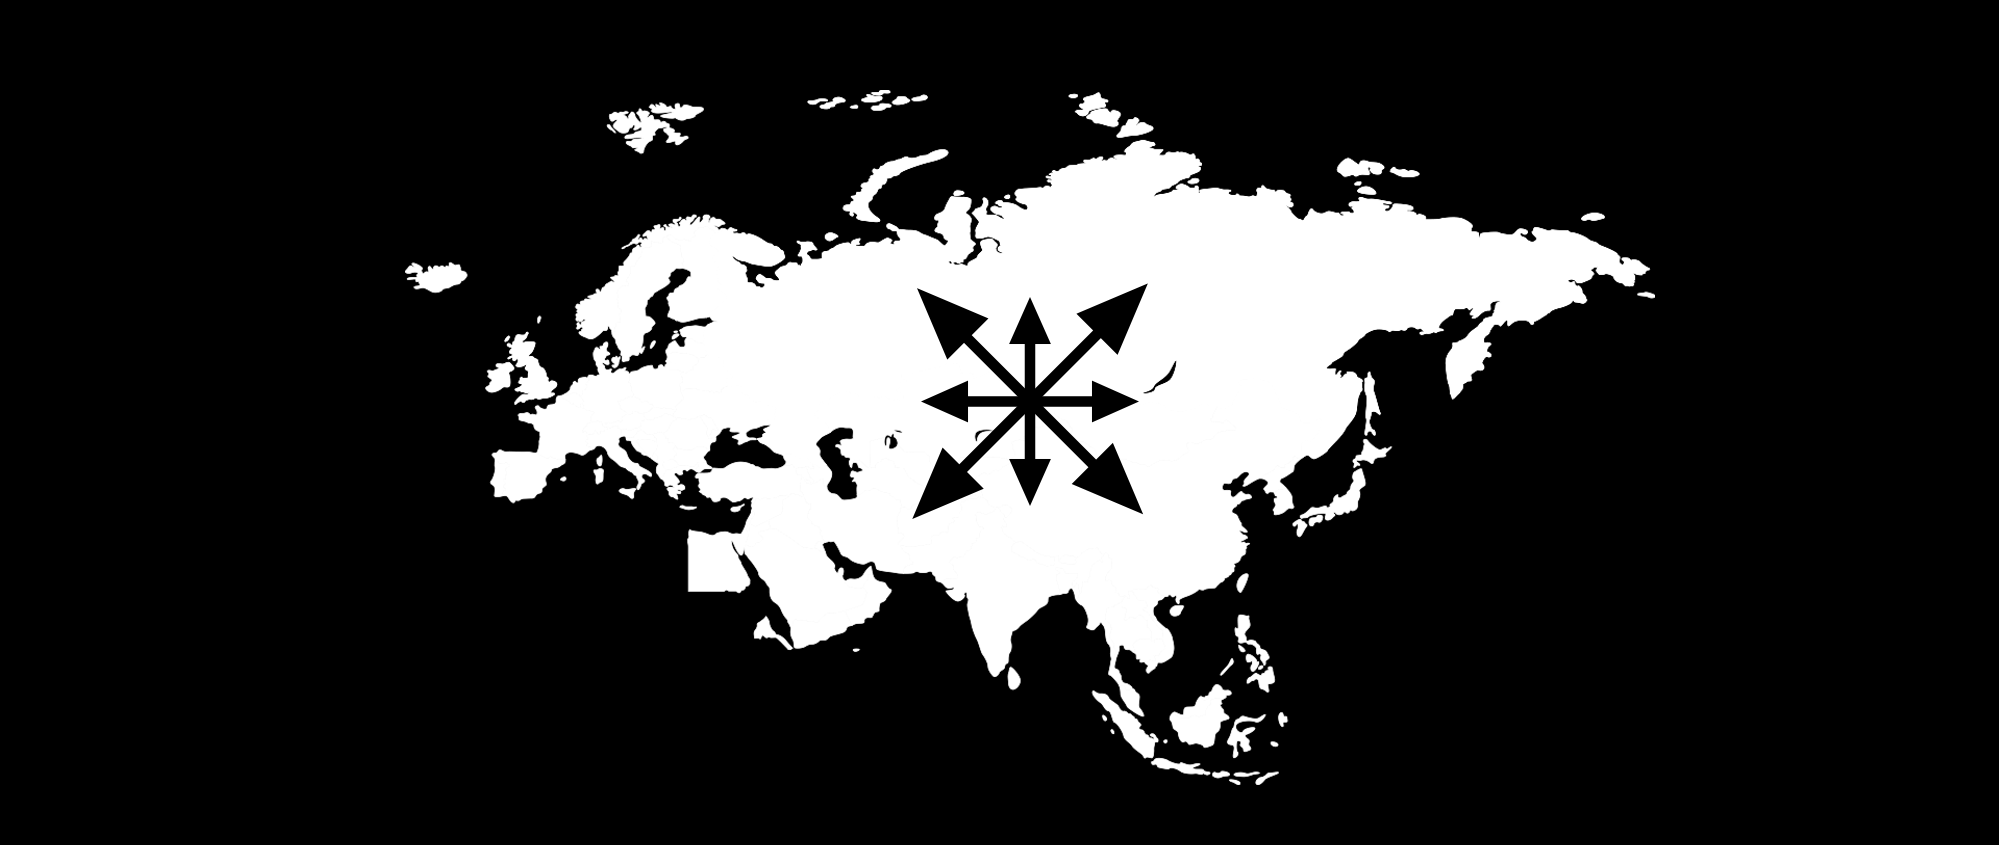
\includegraphics[width=\textwidth]{cover.png}}

\author{Aleksandr Dugin}
\title{Foundations of Geopolitics}

\begin{document}

\maketitle
%Moscow, Arktogeia, 2000

\shipout\null

Translation by Lawless v0 2022-02-26.\\
Original version from Russian, Moscow, Arktogeia, 2000.\\
Author: Aleksandr Dugin\\
%Original title: Основы геополитики - геополитическое будущее России.Osnovy geopolitiki: geopoliticheskoe budushchee Rossii.\\ % I can't get the cyrillic to print correctly. 
Country: Russia\\
Language: Russian\\
Publisher: Arktogeja\\
Publication date: 1997\\
ISBN: 978-5-8592-8019-3.

\tableofcontents
\clearpage


\textbf{From the editors}

The history and fate of geopolitics as a science is paradoxical. On the
one hand, the concept itself seems to have become commonplace, actively
used in contemporary politics. Geopolitical journals and institutions
are proliferating. The texts of the founders of the discipline are
published and republished, conferences and symposia are held, and
geopolitical committees and commissions are established. 

Nevertheless, geopolitics has so far failed to make it into the category
of the conventional conventional conventional sciences. The first
geopolitical works of the German Ratzel, the Swede Chellen, and
especially of the Englishman Mackinder were all greeted with hostility
by the scientific community. Classical scholarship, inheriting the
hypercritical spirit of early positivism, believed that geopolitics
pretended to overgeneralise and was therefore only a form of
"quackery".

In a way, the sad fate of geopolitics as a science was also linked to
the political side of the issue. It has been argued that the war crimes
of the Third Reich - expansion, wars, deportations, etc. - were largely
theoretically prepared by German geopoliticians, who allegedly provided
Hitler's regime with a pseudoscientific basis. (This referred primarily
to Karl Haushofer, a German geopolitical scientist who was at one time
quite close to the Führer.)

However, on a theoretical level German geopolitics was essentially no
different from Anglo-Saxon (Mackinder, Mahan, Speekman), French (Vidal
de la Blanche), Russian "military geography" (Miliutin, Snesarev), etc.
The difference lay not in the specific views of Haushofer, which were
perfectly logical and adequate to the discipline itself, but in the
methods by which a number of his geopolitical positions were
implemented. Moreover, the specificity of German international policy in
the 30s and 40s in its most repellent manifestations sharply
contradicted the ideas of Haushofer himself. Instead of a "continental
bloc" on the Berlin-Moscow-Tokyo axis, an attack on the USSR, instead of
an organicist (in the spirit of the Schmittian theory of "rights of
nations") understanding of the doctrine of Lebensraum, "living space",
vulgar nationalism and imperialism, etc. It should also be noted that
the Haushofer School and its journal "Zeitschrift fur Geopolitik" were
never elements of the official Nazi system. Like many intellectual
groups of the so-called "conservative revolutionaries" in the Third
Reich, they led an ambiguous existence and were simply tolerated, a
tolerance which varied according to the current political situation. 

However, the main reason for the historical oppression of geopolitics is
the fact that it is too explicit in showing the fundamental mechanisms
of international politics, which various regimes most often prefer to
hide behind vague rhetoric or abstract ideological schemes. In this
sense, a parallel can be drawn with Marxism (at least in its purely
scientific, analytical part). Just as Marx more than convincingly
reveals the mechanics of production relations and their relationship to
historical formations, geopolitics exposes the historical demagogy of
foreign policy discourse, showing the real underlying levers that
influence international, interstate and interethnic relations. But while
Marxism is a global revision of classical economic history, geopolitics
is a revision of the history of international relations. This last point
explains the ambivalent attitude of society towards geopolitical
scientists. The scientific community stubbornly rejects them in its
environment, harshly criticising them and, more often than not,
overlooking them, while the authorities, on the contrary, actively use
geopolitical concepts to formulate international strategy. This was the
case, for example, with one of the first geopoliticians, Sir Halford
Mackinder, the true founding father of the discipline. His ideas were
not accepted in academic circles, but he himself was directly involved
in shaping British policy in the first half of the twentieth century,
laying the theoretical foundation for England's international strategy,
taken over by the United States by mid-century and developed by
Mackinder's American (more broadly, Atlanticist) followers. 

The parallel with Marxism is, in our view, apt. The method can be
borrowed and assimilated by different poles. Marxist analysis is equally
important to the representatives of Capital and the fighters for the
emancipation of Labour. So too is geopolitics: it instructs the
representatives of big states (empires) on how best to maintain
territorial domination and carry out expansion, while their opponents
find in it the conceptual principles of a revolutionary theory of
"national liberation". The Treaty of Versailles, for example, was the
work of the geopolitical school of Mackinder, expressing Western
interests and aiming to weaken the states of Central Europe and suppress
Germany. The German disciple of Mackinder, Karl Haushofer, based on the
same premises, developed the exact opposite theory of "European
liberation", which was a complete negation of the logic of Versailles
and formed the basis of the ideology of the nascent National
Socialism.

Recent considerations show that even without being accepted in the
commonwealth of classical sciences, geopolitics is extremely effective
in practice, and its importance in some respects surpasses many
conventional disciplines.

Nevertheless, geopolitics exists today and is slowly gaining official
recognition and status. However, not everything is smooth in this
process either. We are very often confronted with a substitution of the
very notion of geopolitics. We have seen an increasing substitution of
the term geopolitics, which is becoming increasingly commonplace among
laypeople. Emphasis is being shifted from the comprehensive and global
picture developed by the founding fathers to private regional aspects or
geo-economic schemes. The original postulates of geopolitical dualism,
competition of strategies, civilizational differentiation, etc. are
either ignored, glossed over or denied altogether. It is difficult to
imagine something similar in any other science. What would happen to
classical physics if, operating with the concepts of "mass", "energy",
"acceleration", etc., scientists began to implicitly, gradually deny the
law of universal gravitation, forget about it, and then simply
recognized Newton as a "mythological figure who did not exist in
reality" or a "dark religious fanatic". But that, mutatis mutandis, is
what is happening to geopolitics these days. 

The aim of this book is to present basic geopolitics objectively and
impartially, beyond preconceived notions and ideological sympathies and
antipathies. No matter how we feel about this science, we can only make
a definitive judgment about it after becoming familiar with its
principles, history and methodology.






\textbf{INTRODUCTION}

\textbf{The definition of 'geopolitics'}

\hfill\break
The works of numerous representatives of geopolitical schools, despite
all their differences and often contradictions, form a common picture,
which allows us to speak about the subject itself as something complete
and definite. Various authors and dictionaries differ in their
definition of the main subject matter of this science and its main
methodological principles. This divergence stems from historical
circumstances as well as from the close connection of geopolitics with
global politics, issues of power and dominant ideologies. The synthetic
nature of the discipline implies the inclusion of many additional
subjects in geography, history, demography, strategy, ethnography,
religious studies, ecology, military studies, history of ideology,
sociology, political science, etc. Since all these military, natural
sciences and humanities have many schools and trends, we cannot speak of
any strictness and unambiguity in geopolitics. But what definition
should we give to this discipline, which is so vague and at the same
time expressive and impressive? 

Geopolitics is a worldview, and as such is better compared not with
sciences, but with systems of sciences. It is on the same level as
Marxism, liberalism, etc., i.e. systems of interpretations of society
and history that single out one crucial criterion as the main principle
and reduce all other myriad aspects of man and nature to it.

Marxism (1) and liberalism equally put the economic side of human
existence, the principle of "economy as destiny", at the core. Never
mind that the two ideologies draw opposite conclusions Marx arrives at
the inevitability of the anti-capitalist revolution, while Adam Smith's
followers regard capitalism as the most perfect model of society. In
both cases an extended method of interpreting the historical process, a
particular sociology, anthropology and political science are offered.
And despite the constant criticism of these forms of "economic
reductionism" by alternative (and marginal) scientific circles, they
remain the dominant social models on the basis of which people do not
simply make sense of the past, but also create the future, i.e. plan,
design, conceive and carry out large-scale acts which directly affect
all humanity. 

The same is true of geopolitics. But unlike "economic ideologies", it is
based on the thesis: "geography as destiny". Geography and space appear
in geopolitics in the same function as money and production relations in
Marxism and liberalism, they reduce all fundamental aspects of human
existence to them; they serve as a basic method of interpretation of the
past, they act as major factors of human existence, organizing around
themselves all other aspects of existence. Like economic ideologies,
geopolitics is based on approximation, on reductionism, on reducing the
diverse manifestations of life to a few parameters, but despite the
inherent fallacy of such theories, they have proved impressively
coherent in explaining the past and extremely effective in organizing
the present and projecting the future. 

If we continue the parallel with Marxism and classical bourgeois
political economy, we can say that, like economic ideologies, which
affirm the special category of "human economic" (homo economicus),
geopolitics speaks about "human space", predetermined by space, shaped
and conditioned by its specific quality of relief, the landscape. But
this conditionality is especially evident in large-scale social
manifestations of man in states, ethnic groups, cultures, civilizations,
etc. The dependence of each individual on the economy is evident in both
small and large proportions. Therefore, economic determinism is
understandable both to ordinary people and to the authorities operating
with big social categories. This may be the reason why economic
ideologies have become so popular and have performed a mobilising
function up to and including revolutions based on the personal
engagement in the ideology of a multitude of individuals. The dependence
of the individual on space is the main thesis of geopolitics, seen only
at some distance from the individual. This is why, despite its premises,
geopolitics has not become an ideology proper or, more precisely, a
"mass ideology". Its conclusions and methods, subjects of study and
basic theses are intelligible only to those social authorities who are
engaged in large-scale problems of strategic planning, comprehension of
global social and historical regularities, etc. Space manifests itself
in large dimensions, and therefore geopolitics is reserved for social
groups dealing with generalised realities of countries, nations, etc.


Geopolitics is a worldview of power, a science of power and for power.
Only as one gets closer to the social top does geopolitics begin to
reveal its significance, its meaning and its usefulness for one, whereas
before that it is perceived as an abstraction. Geopolitics is the
discipline of political elites (both actual and alternative), and its
entire history provides convincing evidence that it has been practiced
exclusively by people actively involved in the process of governing
countries and nations, or preparing for this role (if alternative,
oppositional ideological camps have been removed from power due to
historical conditions). 

Without claiming scientific rigour, geopolitics at its own level
determines what is of value to it and what is not. The humanities and
the natural sciences are only involved when they do not contradict the
basic principles of the geopolitical method. Geopolitics, in a way,
selects those sciences and branches of science that seem useful to it,
leaving out the rest. In today's world, it is a "ruler's quick reference
book", a textbook of power, which gives a summary of what should be
considered when making global (momentous) decisions such as making
alliances, starting wars, implementing reforms, restructuring society,
imposing massive economic and political sanctions, etc. 

\emph{Geopolitics is the science of ruling.}\\


\textbf{Tellurocracy and Thalassocracy}


The main law of geopolitics is the assertion of a fundamental dualism,
reflected in the geographical structure of the planet and in the
historical typology of civilisations. This dualism is expressed in the
opposition between "tellurocracy" (land power) and "thalassocracy"
(maritime power). The nature of this opposition is reduced to the
opposition of a mercantile civilization (Carthage, Athens) and a
military-authoritarian civilization (Rome, Sparta). In other terms, the
dualism between "democracy" and "ideocracy".

Already from the outset this dualism has the quality of hostility, of
the alternativity of its two constituent poles, although the degree may
vary from case to case. The entire history of human societies is thus
seen as consisting of two elements "aqueous" ("liquid", "fluid") and
"terrestrial" ("solid", "permanent").

"Tellurocracy", "land power" is associated with the fixity of space and
the stability of its qualitative orientations and characteristics. At
the civilizational level, it is embodied in sedentarism, in
conservatism, in strict legal norms, to which large associations of kin,
tribes, nations, states, empires are subjected. The hardness of the
Dryland is culturally embodied in the firmness of ethics and the
stability of social traditions. The dryland peoples (especially
sedentary ones) are alien to individualism and entrepreneurial spirit.
They are characterised by collectivism and hierarchy. 

"Thalassocracy", "maritime power" represents a type of civilisation
based on opposing attitudes. This type is dynamic, mobile and inclined
towards technical development. Its priorities are nomadism (especially
navigation), trade, and the spirit of individual entrepreneurship. The
individual, as the most mobile part of the collective, is elevated to
the highest value, while ethical and legal norms become diluted,
relative and mobile. This type of civilization develops rapidly, evolves
actively, easily changes external cultural attributes, keeping unchanged
only the internal identity of the general attitude. 

Most of human history unfolds in a situation of limited scale of both
orientations under the global dominance of "tellurocracy". The Earth
element (Land) dominates the entire ensemble of civilisations, while the
Water element (sea, ocean) appears only fragmentarily and sporadically.
The dualism remains geographically localised up to a certain point -
seashores, estuaries and river basins, etc. The opposition develops in
different zones of the planet with different intensity and in different
forms. 

The political history of the peoples of the earth shows a gradual growth
of political forms becoming more and more extensive. This is how states
and empires emerge. This process on the geopolitical level means the
strengthening of the factor of space in human history. The nature of
large political formations of states and empires expresses the duality
of the elements more impressively, reaching the level of more and more
universal civilizational types. 

At a certain point (the ancient world) a rather stable picture emerges,
reflected in the "Mackinder map". The Tellurocracy zone is steadily
identified with the inland expanses of NorthhEastern Eurasia (which in
general terms coincide with the territories of Tsarist Russia or the
USSR). Thalassocracy is increasingly being identified as the coastal
zones of the Eurasian continent, the Mediterranean area, the Atlantic
Ocean and the seas that bathe Eurasia from the South and West. 

This is how the world map becomes geopolitically specific: 

\emph{1) Intra-continental spaces become a "fixed platform", a
"heartland", a "geographical axis of history" which steadily preserves
the telluric civilisational specificity.} 

\emph{2) The "inner or continental crescent", the "coastal zone", the
rimland represents a space of intense cultural development. Features of
"Thalassocracy" are evident here. Although they are counterbalanced by
many "telluric" tendencies.} 

\emph{3) The "outer or island crescent" represents "uncharted lands"
with which only maritime communication is possible. It first makes
itself known in Carthage and the trading Phoenician civilisation,
affecting the "inner crescent" of Europe from outside.}

This geopolitical picture of the relationship between thalassocracy and
tellurocracy is revealed potentially at the beginning of the Christian
era, after the Punic Wars. But it finally makes sense in the period when
England became a great maritime power in the seventeenth and nineteenth
centuries. The era of great geographical discoveries, which began at the
end of the fifteenth century, entailed the final establishment of
Thalassocracy as an independent planetary entity that broke away from
Eurasia and its shores and concentrated entirely in the Anglo-Saxon
world (England, America) and the colonies. The "New Carthage" of
Anglo-Saxon capitalism and industrialism took shape as a single entity,
and from then on geopolitical dualism acquired clearly distinguishable
ideological and political forms. 

England's positional struggle with the continental powers of the
Austro-Hungarian Empire, Germany and Russia was the geopolitical content
of the 17th and 19th centuries (+ second half of the 20th century), and
since the middle of our century, the main stronghold of Thalassocracy
has been the USA. 

In the Cold War of 1946-1991, the perennial geopolitical dualism reached
maximum proportions, Thalassocracy identified with the USA and
Tellurocracy with the USSR. 

The two global types of civilisation, culture and meta-ideology have
developed into complete geopolitical outlines, summarising the entire
geopolitical history of the confrontation of the elements. However, it
is striking that these forms of complete geopolitical dualism on the
ideological level were matched by two equally synthetic realities, the
ideology of Marxism (socialism) and the ideology of liberal-capitalism.


In this case, we can speak of the realisation in practice of two types
of "reductionism": economic reductionism was reduced to the opposition
between Smith's ideas and Marx's ideas, and geopolitical reductionism to
the division of all sectors of the planet into zones controlled by
thalassocracy (New Carthage, USA) and tellurocracy (New Rome, USSR).

The geopolitical vision of history is a model of the development of
planetary dualism to maximum proportions. Land and Sea extend their
original opposition to the entire world. 

Human history is nothing more than an expression of this struggle and a
path to its absolutisation. 

This is the most general expression of the main law of geopolitics, the
law of dualism of the elements (Land versus Sea).\\


\textbf{Geopolitical teleology}


Until the final victory of the United States in the Cold War,
geopolitical dualism had been developing within an inherently
pre-determined framework: thalassocracy and tellurocracy were gaining
maximum spatial, strategic and force volume. As both sides were building
up their nuclear capabilities, to some pessimistic geopoliticians the
outcome of this process seemed catastrophic, since, having fully
mastered the planet, the two powers would either have to transfer the
confrontation beyond the earth (Star Wars theory) or mutually destroy
each other (nuclear apocalypse). 

If the nature of the main geopolitical process of history the maximum
spatial expansion of thalassocracy and tellurocracy is clear to this
discipline, its outcome remains in question. There is no determinism in
this respect. 

Consequently, geopolitical teleology, i.e. thinking about the purpose of
history in geopolitical terms, only reaches the point of globalising
dualism and stops there. 

Nevertheless, on a purely theoretical level, a number of hypothetical
versions of developments can be deduced, once one of the two systems of
thalassocracy has triumphed. 

\emph{Option 1} . The victory of Thalassocracy completely abolishes
Tellurocracy civilisation. A homogeneous liberal-democratic order is
established on the planet. Thalassocracy absolutizes its archetype and
becomes the only system of organization of human life. This variant has
two advantages: firstly, it is logically consistent, because one can see
in it the natural completion of the unidirectional (in general) flow of
geopolitical history from the complete domination of the Land
(traditional world) to the complete domination of the Sea (modern
world); and secondly, this is what is happening in reality. 

\emph{Option 2} . The victory of thalassocracy ends the cycle of
confrontation between the two civilisations, but it does not extend its
model to the whole world, but simply ends geopolitical history,
cancelling its problematics. Just as the theories of post-industrial
society prove that the basic contradictions of classical political
economy (and Marxism) are removed in this society, so some monist
theories argue that in the coming world the land-sea confrontation will
be removed altogether. This too is the "end of history", only further
developments do not lend themselves to the same rigorous analysis as in
the first version. 

Both of these analyses treat the defeat of the Tellurocracy as an
irreversible and fait accompli. Two other analyses treat it differently.


\emph{Option 3} . The defeat of the tellurocracy is a temporary
phenomenon. Eurasia will return to its continental mission in a new
form. The geopolitical factors that led the continentalist forces to
catastrophe will be taken into account (the new continental bloc will
have maritime borders to the South and West, i.e. the "Monroe Doctrine
for Eurasia" will be implemented). In that case, the world would return
to bipolarity. But of a different quality and level.

\emph{Option 4} (which is a development of the previous one). In this
new confrontation, tellurocracy wins. It seeks to transfer its own
civilisation model to the entire planet and "close history" on its
chord. The whole world will typologically become Dryland and "ideocracy"
will reign everywhere. A foretaste of this outcome was the idea of a
"World Revolution" and the planetary domination of the Third Reich. 

Since the role of the subjective and rational factor in the development
of historical processes is greater than ever before, the four options
should not be seen simply as an abstract statement of the likely
development of the geopolitical process, but as active geopolitical
positions that can guide action on a global scale. 

But in this case, geopolitics cannot offer any deterministic version. It
comes down to a set of possibilities, the realisation of which will
depend on a variety of factors that no longer fit into a purely
geopolitical analysis.\\


\textbf{Rimland and 'border zones'}


The entire methodology of geopolitical research is based on the
application of the principles of the global geopolitical dualism of Land
and Sea to more local categories. In the analysis of any situation, it
is the planetary model that remains central and fundamental. Those
relations that are characteristic of the overall picture are also
repeated at a more private level. 

After highlighting the two basic principles of thalasso cratia and
tellurocracy, the next most important principle is rimland, the "coastal
zone". This is a key category underlying geopolitical research.

Rimland is a composite space that potentially carries the possibility of
being a fragment of either thalassocracy or tellurocracy. It is the most
complex and culturally saturated region. The influence of the marine
element, Water, provokes an active and dynamic development in the
"coastal zone". The continental mass presses, forcing the structuring of
energy. On the one hand, rimland passes into Island and Ship. On the
other side into Empire and Home. 

Rimland is not, however, merely an intermediate and transitional
environment in which the opposition between the two impulses plays out.
It is a very complex reality, with a logic of its own and with an
enormous influence on both Thalassocracy and Tellurocracy. It is not the
object of history, but its active subject. The struggle for the rimland
of Thalassocracy and Tellurocracy is not a contest for the possession of
a mere strategic position. Rimland has a destiny of its own and its own
historical will, which, however, cannot be resolved outside of a basic
geopolitical dualism. Rimland is largely free to choose, but not free in
the structure of the choice, because apart from the thalassocratic or
telluric path it has no third one. 

Because of this quality, the 'inner crescent' is often identified with
the areal extent of human civilisation in general. In the interior of
the continent conservatism reigns, outside its borders the challenge of
fluid chaos. 

Coastal zones, by their very position, are confronted with the need to
provide an answer to the problem posed by geography. 

Rimland is a border zone, a belt, a strip. At the same time it is a
borderland. This combination leads to a geopolitical definition of the
border.

In contrast to borders between states, geopolitics understands the term
differently, starting from the original model in which the first border
or archetype of all borders is a specific historical-geographical and
cultural concept of rimland. 

The spatial extent of the coastal zones is a consequence of looking at
the mainland from outside, "from the face of the sea aliens". It is for
the "forces of the sea" that the coast is \emph{a strip} extending
inland. For the mainland itself, by contrast, the shore is the limit,
the \emph{line}. 

The border as a line (which is how it is understood in international
law) is a vestige of "land jurisprudence" inherited by modern law from
ancient traditions. It is a purely land-based view. 

But the maritime view, external to the mainland, sees coastal
territories as potential colonies, as strips of land which can be torn
away from the rest of the continent, turned into a base, a strategic
space. At that, the coastal zone is never completely "one's own"; if
necessary, one can take a ship and sail away to one's home, to the
"island". The shoreline becomes a strip precisely because it is unsafe
for aliens from the sea to go only a certain distance into the interior
of the continent.

Since geopolitics combines both views of space maritime and land, it
understands the rimland as a special reality, as a border-band, with its
qualitative volume depending on which impulse dominates the sector, land
or sea. The giant and quite navigable ocean shores of India and China
are lines, strips of minimal volume. The cultures concerned are
land-oriented, and the volume of the coastal strips gravitates towards
zero, towards being simply the end of the continent. In Europe and
particularly in the Mediterranean the coastal zones are broad strips
extending far inland. Their volume is at its maximum. However in both
cases we are talking about a geopolitical frontier. It is therefore a
variable category, varying from line to line, depending on the
circumstances. 

This approach is also projected by geopolitics into the analysis of more
specific problems related to borders. It views borders between states as
"zones of variable volume". This volume its contraction or expansion
depends on general continental dynamics. Depending on it, these zones
change shape and trajectory within given limits. The notion of
"geopolitical frontier" may include entire states. For example, the
British idea of a "cordon sanitaire" between Russia and Germany
envisaged the creation of a "no-man's zone" (semi-colonial and oriented
towards England) consisting of the Baltic and Eastern European states.
By contrast, the continentalist policies of Russia and Germany
gravitated towards turning this zone into a line (Brest-Litovsk,
Rappalo, the Ribbentrop-Molotov Pact). The Thalassocrats-Atlanteans
sought to extend it as far as possible by creating artificial
"pro-strategic states" (etats-tampons). 

In this case, the complete and perfect thalassocracy (England, the
United States) applies a double standard: the thalassocrats seek to
reduce the borders of their own islands to a line, and the coastal zones
of Eurasia to the maximum extent possible. For continentalist
geopolitics, it is logical to use exactly the same principle in the
opposite direction: Eurasian borders line, American borders strip. 

The analogy with the historical rimland as the 'cradle of civilisation'
shows the crucial importance of 'frontier zones' in more specific cases
as well. Free from the need to bear the weight of the geographical
charge of history, 'frontier zones' often channel their energy into
cultural-intellectual spheres. And the skilful use of this "easy"
geopolitical potential constitutes the art of the geopolitical strategy
of the opposing sides. 

It was the "maritime force" that had mastered this to perfection, as it
had always been based on the principle of making the most of colonised
territories as quickly as possible. This distinguished them from land
invaders who, once they had conquered a territory, immediately began to
regard it as their own and, therefore, were in no hurry to squeeze what
they could out of it.\\


\textbf{Geopolitics as destiny}


The laws of geopolitics are extremely useful for analysing political
history, the history of diplomacy and strategic planning. This science
has many intersections with sociology, political science, ethnology,
military strategy, diplomacy, history of religions, etc. Indirectly, but
at times very clearly, it is also linked to economics, to the extent
that some geopoliticians have proposed the establishment of a new
science of geoeconomics. In any case, in some aspects of the
geopolitical method, reference to economic realities is necessary. 

At present, with all kinds of sciences gravitating towards synthesis,
towards fusion, towards creation of new interscientific
macro-disciplines and multi-dimensional models, geopolitics reveals its
importance both for purely theoretical research and for practical steps
in managing complex civilizational processes on a planetary scale or on
the scale of individual states or blocs of states. This is a science of
the future, the foundations of which will soon be taught not only in
special institutions of higher education and academies, but also in
elementary schools. With the help of geopolitical analysis we may easily
comprehend entire epochs of historical development of nations and
peoples. With the expansion of information zones inherent in our time,
the emergence of such simple and clear reductionist methodologies is
inevitable, because otherwise one risks finally losing all reference
points in the diverse and multidimensional chaos of flows of
heterogeneous knowledge. 

Geopolitics is an invaluable aid to education. Its structure is such
that it could become an axial discipline in the new stage of school
development. 

At the same time, the role of geopolitics in the wider social sphere is
becoming increasingly evident. The level of information development, the
active involvement of the common man in the events unfolding on the
whole continent, the "monedialization" of the mass media all bring to
the fore spatial thinking in geopolitical terms, which helps to "sort"
nations, states, regimes and religions on a single simplified scale in
order to make even the most basic TV or radio news at least
approximately understandable. If one applies the simple geopolitical
grid of heartland, rimland, World Island to any report concerning
international events, a clear interpretative model is immediately built
up, requiring no additional highly specialized knowledge. "NATO
enlargement to the East" in this approach means "an increase in rimland
in favour of Thalassocracy"; "an agreement between Germany and France
regarding the creation of a special purely European military force" "a
step towards the creation of a continental telluric construct"; "the
conflict between Iraq and Kuwait the desire of the continental state to
destroy the artificial Thalassocratic formation preventing direct
control of the coastal zone", etc. 

Finally, the impact of geopolitical methodology on domestic and foreign
policy. If the geopolitical meaning of certain steps taken by political
parties and movements as well as power structures is evident, it is easy
to relate them to the system of global interests, and hence to decipher
their far-reaching goals. For example, the integration of Russia with
European countries (especially Germany) is a step of the tellurist
(Eurasianist) forces, hence the strengthening of "ideocratic"
("socialist") tendencies within the country can automatically be
predicted. On the contrary, Moscow's rapprochement with Washington means
subordination to the Thalassocratic line and inevitably entails a
positional strengthening of the "marketists", etc. Similarly, the
internal political processes of separatism of peoples within Russia,
bilateral or multilateral agreements of different administrative
formations and regions among themselves can easily be interpreted in the
light of the patterns of internal geopolitics. Every event acquires a
clear meaning in the light of geopolitics. This geopolitical meaning
cannot be regarded as ultimo ratio of an event, but in any case it
proves to be always highly expressive and useful for analysis and
forecasting. 

The lack of any textbook on the subject today prompted us to write and
compile this book, which provides an introduction to geopolitics as a
science. 






\part{PART 1 FOUNDING FATHERS OF GEOPOLITICS}

\chapter{Chapter 1}

\section{Friedrich Ratzel States as spatial organisms}

\textbf{1.1 Education: The German "Organizationalist School}


Friedrich Ratzel (1844 1904) can be considered the "father" of
geopolitics, although he himself did not use the term in his writings.
He wrote about "political geography". His main work, published in 1897,
is called "Politische Geographie". 

Ratzel graduated from the Polytechnic University in Karlsruhe, where he
took courses in geology, palaeontology and zoology. He completed his
education at Heidelberg, where he became a student of Professor Ernst
Goeckel (who was the first to use the term "ecology"). Ratzel's
worldview was based on evolutionism and Darwinism and was coloured by a
pronounced interest in biology. 

Ratzel took part in the war of 1870, where he volunteered and was
awarded the Iron Cross for bravery. In politics he gradually becomes a
convinced nationalist and in 1890 joins the "Pan-Germanist League" of
Karl Peters. He travelled extensively in Europe and America and added
ethnological studies to his academic interests. He becomes a lecturer in
geography at the Technical Institute of Munich, and in 1886 takes a
similar chair in Leipzig. 

In 1876, Ratzel defended his thesis on 'Emigration in China', and in
1882, Stuttgart published his fundamental work, 'Anthropogeographie', in
which he formulates his main ideas: the connection between the evolution
of peoples and demography and geographic data, the influence of
topography on the cultural and political formation of peoples, etc.

But his most important book was Political Geography.\\


\subsection{1.2 States as living organisms}


In this work Ratzel shows that soil is the fundamental, unchanging datum
around which the interests of peoples revolve. The movement of history
is predetermined by soil and territory. This is followed by the
evolutionist conclusion that "the state is a living organism", but an
organism "rooted in the soil". The state is constituted by territorial
topography and scale and by the people's comprehension of them. The
state thus reflects an objective geographical given and a subjective
national comprehension of this given, expressed in policy. Ratzel
considers a 'normal' state to be the one which most organically combines
the geographical, demographic and ethno-cultural parameters of a nation.


He writes\\


"\emph{States, at all stages of their development, are seen as organisms
which necessarily retain a connection with their soil and must therefore
be studied from a geographical point of view. As ethnography and history
show, states develop on a spatial basis, becoming more and more
contiguous and merging with it, deriving more and more energy from it.
Thus, states turn out to be spatial phenomena governed and animated by
that space; and it is up to geography to describe, compare and measure
them. States fit into the series of phenomena of the expansion of Life,
being the highest point of these phenomena}" ("Political Geography"
(1)).


From this 'organicist' approach it is clear that the spatial expansion
of the state is understood by Ratzel as a natural living process,
similar to the growth of living organisms. 

Ratzel's 'organic' approach is also reflected in the relation to space
itself (Raum). This "space" changes from a quantitative material
category to a new quality, becoming \emph{a} "\emph{vital sphere}", a
"\emph{vital space}" (Lebensraum), a kind of
"\emph{geobio-environment}". Hence Ratzel's other two important terms
"\emph{spatial sense}" (Raumsinn) and "\emph{vital energy}"
(Lebensenergie). These terms are close to each other and denote a
certain special quality inherent in geographical systems and
predetermining their political formation in the history of peoples and
states. 

All these theses are the underlying principles of geopolitics, in the
form in which it will be developed later by Ratzel's followers.
Moreover, the attitude towards the state as a "\emph{living, natural
organism rooted in the soil}" is the main idea and axis of the
geopolitical methodology. This approach focuses on the synthetic study
of the whole complex of phenomena, whether they belong to the human or
non-human sphere. Space, as a concrete expression of nature, the
environment, is seen as a continuous vital body of the ethnos that
inhabits this space. The structure of the material itself dictates the
proportions of the final work of art. 

In this sense, Ratzel is a direct heir to the whole school of German
"organic" sociology, of which Ferdinand Tennys was the most prominent
spokesman.\\


\subsection{1.3. Raum political organisation of the soil}


How Ratzel saw the relationship between ethnicity and space can be seen
in the following fragment of Political Geography: 

"\emph{The state is formed as an organism attached to a certain part of
the surface of the earth, and its characteristics develop from the
characteristics of the people and the soil. The most important
characteristics are size, location and boundaries. Next are the types of
soil together with vegetation, irrigation, and finally the relations
with the rest of the conglomerates of the earth's surface, and above all
with the adjacent seas and uninhabited lands, which, at first sight, are
not of much political interest. The aggregate of all these
characteristics constitutes a country (das Land). But when one speaks of
"our country", to this is added all that man has created and all the
memories associated with the land. This is how an initially purely
geographical concept is transformed into a spiritual and emotional
connection between the inhabitants of the country and their history.}

\emph{The State is an organism not only because it articulates the life
of the people on fixed ground, but because this bond is mutually
reinforcing, becoming something unified, unthinkable without one of the
two components. Uninhabited space, unable to nurture the State, is a
historical field under steam. An inhabited space, on the contrary, is
conducive to the development of the state, especially if this space is
surrounded by natural borders. If a people feel its territory naturally,
it will constantly reproduce the same characteristics that, originating
from the soil, will be inscribed in it}."(2) { }

\subsection{1.4 The law of expansion}


Treating the state as a living organism implied a rejection of the
concept of "inviolability of borders". The state is born, grows and dies
like a living being. Consequently, its spatial expansion and contraction
are natural processes associated with its internal life cycle. Ratzel,
in his book "On the Laws of Spatial Growth of States" (1901)
distinguished \emph{seven laws of expansion} :

\textbf{1) The extent of the States increases as their culture
develops;}

\textbf{2) The spatial growth of the state is accompanied by other
manifestations of its development: in the fields of ideology,
production, commercial activity, powerful "attractional radiation",
proselytism.}

\textbf{3) The state expands by absorbing and absorbing political units
of lesser importance.}

\textbf{4) The border is an organ located on the periphery of the State
(understood as an organism).}

\textbf{5) In its spatial expansion, the State seeks to cover the most
important regions for its development: coasts, river basins, valleys and
generally all rich territories.}

\textbf{6) The initial impetus for expansion comes from outside, as the
State is provoked into expansion by a state (or territory) with a
clearly inferior civilisation.}

\textbf{7) The general tendency to assimilate or absorb weaker nations
pushes for even more territory in a movement that feeds on
itself.}(3)

Not surprisingly, many critics have reproached Ratzel for writing
'Catechism for Imperialists'. Yet Ratzel himself did not seek to justify
German imperialism by any means, although he made no secret of his
nationalist convictions. For him, it was important to create a
conceptual tool for an adequate understanding of the history of states
and peoples in their relation to space. In practice, however, he sought
to arouse "Raumsinn" ("\emph{sense of space}") in the German leaders,
for whom the geographical data of dry academic science had often
appeared as pure abstraction.\\


\subsection{1.5 Weltmacht and the sea}


Ratzel was greatly influenced by his familiarity with North America,
which he studied well and to which he dedicated two books: Maps of North
American Cities and Civilization (1874). (1874) and "The United States
of North America" (1878 1880). He noted that the Americans had a "high
sense of space" because they were confronted with the challenge of
"empty" spaces, having a considerable \emph{"politico-geographical"}
experience in European history. Consequently, the Americans consciously
carried out what the Old World had arrived at intuitively and gradually.
Thus, in Ratzel we encounter the first formulations of another major
geopolitical concept, that of '\emph{world power}' (Weltmacht). Ratzel
noticed that large countries in their development have a tendency
towards maximum geographical expansion, gradually reaching a planetary
level. 

Consequently, sooner or later, geographical development is bound to
approach its continental phase. 

Applying this principle, derived from the American experience of
political and strategic continental unification, to Germany, Ratzel
foresaw the fate of a continental power. 

He also anticipated another major geopolitical theme, the importance of
the sea in the development of civilisation. In his book "The Sea, Source
of the Power of Nations" (1900)(4). (1900)(4) he pointed out the
necessity for every powerful nation to especially develop its naval
forces, as the planetary scale of full-fledged expansion demands it.
What some nations and states (England, Spain, Holland, etc.) have done
spontaneously, the land powers (Ratzel was naturally referring to
Germany) must do deliberately: developing the navy is a prerequisite for
approaching the status of "world power" (Weltmacht). 

The sea and the "world power" are already linked in Ratzel's work,
although it is only in later geopoliticians (Mahan, Mackinder,
Haushofer, especially Schmitt) that this theme will gain completeness
and centrality. 

Ratzel's writings are a necessary basis for all geopolitical studies. In
a condensed form, his writings contain almost all of the basic theses
that will form the basis of this science. The Swede Chellen and the
German Haushofer based their concepts on Ratzel's books. His ideas were
taken into account by the Frenchman Vidal de la Blanche, the Englishman
Mackinder, the American Mahan and the Russian Eurasians (P.Savitsky,
L.Gumilev, etc.). 

It should be noted that Ratzel's political sympathies are not
accidental. The geopoliticians were almost all marked by a strong sense
of nationality, whether it took the form of democracy (the Anglo-Saxon
geopoliticians Mackinder and Mahan) or "ideocracy" (Haushofer, Schmitt,
the Eurasians). 



\chapter{Chapter 2}

\section{Rudolf Schellen and Friedrich Naumann Middle Europe}

\subsection{2.1 The definition of new science}


The Swede Rudolf Chellen (1864 1922) was the first to use the term
"geopolitics".

He was a professor of history and political science at the universities
of Uppsala and Gothenburg. He was also active in politics and a member
of parliament, distinguished by an emphatically Germanophile
orientation. He was not a professional geographer and regarded
geopolitics, which he developed from Ratzel's work (he regarded him as
his teacher), as part of political science. 

Chellen defined geopolitics as follows\\


"\emph{It is the science of the State as a geographical organism
embodied in space}" (5).


In addition to "geopolitics", Chellen proposed four other neologisms,
which he thought would constitute the main sections of political
science:

\textbf{eco-politics ("the study of the State as an economic
force");}

\textbf{Demopolitics ("the study of the dynamic impulses transmitted by
the people to the State"; analogous to Ratzel's
"Anthropogeography");}

\textbf{Sociopolitics ("the study of the social aspect of the
State");}

\textbf{Cratopolitics ("the study of forms of government and power in
relation to problems of law and socio-economic factors")} (6).

But all of these disciplines, which Chellen developed in parallel to
geopolitics, were not widely recognised, whereas the term 'geopolitics'
became firmly established in a wide variety of circles.\\


\subsection{2.2 The state as a form of life and Germany's interests}


In his major work The State as a Form of Life (1916)(7), Chellen
developed the postulates of Ratzel's work. Like Ratzel, Chellen saw
himself as a follower of German "organism", which rejected a mechanistic
approach to the state and society. \emph{The rejection of a strict
division of subjects of study into "inanimate objects" (background) and
"human subjects" (actors) is a hallmark of most geopoliticians}. In this
sense, the very title of Chellen's major work is indicative. 

Pellen developed Ratzel's geopolitical principles in relation to the
specific historical situation in Europe today. 

He took Ratzel's idea of a "\emph{continental state}" to its logical
conclusion with regard to Germany. And he showed that in the context of
Europe Germany is the space that possesses axial dynamism and that is
meant to structure the other European powers around itself. Chellen
interpreted World War I as a natural geopolitical conflict between the
dynamic expansion of Germany (the "Axis countries") and the
countervailing peripheral European (and extra-European) states (the
Entente). The different geopolitical dynamics of downward growth for
France and England and upward growth for Germany predetermined the basic
balance of power. At the same time, in his view, the geopolitical
identification of Germany with Europe was inevitable and inescapable,
despite its temporary defeat in the First World War. 

The geopolitical maximal interests of Germany (= the interests of
Europe) are opposed to those of the Western European powers (especially
France and England), as set out by Ratzel. But Germany is a "\emph{young
nation}" and the Germans are a "\emph{young people}". (This idea of
"young nations", which the Russians and Germans were considered to be,
goes back to F. Dostoyevsky, quoted more than once by Chellen.) The
"young" Germans, inspired by the "\emph{middle European space}", should
move towards a continental state on a planetary scale at the expense of
territories controlled by the "\emph{old peoples}" the French and the
English. The ideological aspect of the geopolitical confrontation was
considered by Chellen to be of secondary importance.\\


\subsection{2.3 Towards a Middle European concept}


Although Chellen was himself a Swede, insisting on a rapprochement
between Swedish and German politics, his geopolitical ideas about the
independent integrating value of Germanic space closely followed
Friedrich Naumann's theory of "Middle Europe" (Mitteleuropa). 

In his book "Mitteleuropa" (1915)(8) Naumann made a geopolitical
diagnosis identical to that of Rudolf Chellen. From his point of view,
in order to compete with such organized geopolitical entities as England
(and its colonies), the USA and Russia, the peoples inhabiting Central
Europe have to unite and organize a new integrated political-economic
space. The axis of this space will of course be the Germans. 

Mitteleuropa, unlike the pure Pan-Germanist projects, was no longer a
national concept, but a purely geopolitical one, where the emphasis was
not on ethnic unity, but on a common geographical destiny. Naumann's
project implied the integration of Germany, Austria, the Danubian states
and, in the distant future, France. 

The geopolitical project was also supported by cultural parallels.
Germany itself as an organic entity was identified with the spiritual
concept of "\emph{Mittellage}", the "middle ground". This was
articulated by Arndt as early as 1818 "\emph{God has placed us in the
centre of Europe; we (the Germans) are the heart of our part of the
world}".

Through Chellen and Naumann, Ratzel's "continental" ideas gradually
acquired tangible features. 



\chapter{Chapter 3}

\section{Halford Mackinder "The geographical axis of history"}

\subsection{3.1 Scientist and politician}


Sir Halford J. Mackinder (1861 1947) is the brightest figure among
geopoliticians.

Educated in geography, he taught at Oxford from 1887 until he was
appointed director of the London School of Economics. From 1910 to 1922
he was a member of the House of Commons and in between (1919 1920) as
British envoy to southern Russia. 

Mackinder is renowned for his high standing in the world of British
politics, whose international orientations he has greatly influenced,
and for his bold and revolutionary scheme of interpreting the political
history of the world. 

McInder's example highlights a typical paradox inherent in geopolitics
as a discipline. Mackinder's ideas were not accepted by the scientific
community, despite his high standing not only in politics, but also in
the scientific community itself. Even the fact that for nearly half a
century he was actively and successfully involved in constructing
English strategy in international affairs on the basis of his
interpretation of the political and geographical history of the world,
could not make the sceptics recognize the value and effectiveness of
geopolitics as a discipline.\\


\subsection{3.2 The geographical axis of history}


Mackinder's first and most brilliant presentation was his paper "The
Geographic Axis of History" (9), published in the Journal of Geography
in 1904. In it he set out the basis of his vision of history and
geography, which he developed in later works. This text can be
considered as the main geopolitical text in the history of the
discipline, as it not only summarises all the previous lines of
development of "political geography", but formulates the basic law of
the discipline. 

Mackinder argues that the most advantageous geographical position for
the state would be the middle, central position. Centrality is relative,
and may vary from one geographical context to another. But from a
planetary point of view, at the centre of the world lies the
\emph{Eurasian continent}, and at its centre is the "heartland" or
\emph{"heartland".} Heartland is the concentration of the continental
masses of Eurasia. It is the most favourable geographical base for
controlling the world. 

Heartland is a key territory in a more general context within World
\emph{Island.} In World Island, McInder includes the three continents of
Asia, Africa and Europe. 

In this way, Mackinder hierarchises planetary space through \emph{a
system of concentric circles}. At the very centre is the
"\emph{geographical axis of history}" \emph{or "pivot area}". This
geopolitical concept is geographically identical with \emph{Russia.} The
same "axial" reality is called heartland, "land of the heartland". 

Next is the '\emph{inner or marginal crescent}'\emph{. This belt
coincides with the coastal areas of the Eurasian continent}. According
to Mackinder, the "inner crescent" represents \emph{the} zone of
\emph{the most intensive development of civilization}. This corresponds
to the historical hypothesis that civilization emerged originally on the
shores of rivers or seas, the so-called "\emph{Potamian theory}. It
ought to be stressed that the latter theory is an essential point in all
geopolitical constructions. The intersection of land and water is a key
factor in the history of nations and states. This theme will be
specifically developed further by Schmitt and Spickman, however, it was
Mackinder who first derived this geopolitical formula. 

Then comes the outer circle\emph{: the "outer or insular crescent".}
This is an area entirely \emph{external} (geographically and culturally)
to the mainland mass of World Island.

Mackinder believes that the entire course of history is determined by
the following processes. From the centre of the land to its periphery
there is constant pressure from so-called "\emph{land robbers}". This is
reflected especially clearly and vividly in the Mongol conquests. The
Scythians, Huns, Alans and so on preceded them. Civilisations arising
from the 'geographical axis of history', from the innermost spaces of
the world, have, according to Mackinder, an 'authoritarian',
'hierarchical', 'undemocratic' and 'non-traditional' character. In the
ancient world it is embodied in a society similar to that of Doric
Sparta or ancient Rome. 

From outside, from the regions of the "island crescent", pressure is
exerted on the World Island by the so-called "\emph{sea robbers"} or
"islanders". These are colonial expeditions emanating from an
extra-Eurasian centre, seeking to counterbalance overland impulses
emanating from the inner limits of the continent. The civilisation of
the "outer crescent" is characterised by a "trading" character and
"democratic forms" of politics. In antiquity, the state of Athens or
Carthage had this character. 

Between these two polar civilisational-geographical impulses is the
"inner crescent" zone, which, being dual and constantly experiencing
opposing cultural influences, has been the most fluid and has thus
become the site of the priority development of civilisation. 

History, according to Mackinder, revolves geographically around the
continental axis. It is in the space of the "inner crescent" that this
history is most clearly felt, whereas in the heartland there is a
"frozen" archaism and in the "outer crescent" a kind of civilisational
chaos.\\


\subsection{3.3 Russia's key position}


Mackinder himself identified his interests with those of the Anglo-Saxon
insular world, i.e. with the position of the "outer crescent". In such a
situation he saw the basis of the geopolitical orientation of the
"insular world" in the maximum weakening of the heartland and the
maximum possible expansion of the influence of the "outer crescent" on
the "inner crescent". Mackinder emphasised the strategic priority of the
"geographical axis of history" in all world politics and thus formulated
the most important geopolitical law\\


"He who \emph{controls Eastern Europe dominates the heartland; he who
dominates the heartland dominates the World Island; he who dominates the
World Island dominates the world.} "("Democratic Ideals and Reality")
(10)


On a political level, this meant recognising Russia's leading role in a
strategic sense. Makinder wrote\\


"\emph{Russia occupies as central a strategic position in the whole
world as Germany does with regard to Europe. It can launch attacks in
all directions and is exposed to them from all sides except the north.
It is only a matter of time before its railway capabilities are fully
developed.} "("The Geographic Axis of History") (11)


On this basis, Mackinder believed that the main objective of Anglo-Saxon
geopolitics was to prevent a strategic continental alliance from forming
around the "geographical axis of history" (Russia). Consequently, the
strategy of the "outer crescent" forces is to tear off as many coastal
areas as possible from the heartland and place them under the influence
of an "insular civilisation".\\


\emph{"A shift in the balance of power in favour of the "axis state"
(Russia A.D.), accompanied by its expansion into the peripheral spaces
of Eurasia, would enable the huge continental resources to be used to
create a powerful naval fleet: it would not be far off from being a
world empire. This will be possible if Russia unites with Germany. The
threat of such a development would force France into an alliance with
the overseas powers, and France, Italy, Egypt, India and Korea would
become coastal bases to which the flotillas of the external powers would
dock in order to disperse the Axis forces in all directions and prevent
them from concentrating all their efforts on building a powerful naval
force.} "("The Geographic Axis of History") (12)


Most interestingly, Mackinder was not just building theoretical
hypotheses, but was actively involved in organising international
support for the Entente "white movement", which he saw as an Atlanticist
tendency aimed at weakening the power of the pro-German Eurasian
Bolsheviks. He personally advised the leaders of the White cause,
seeking maximum support from the British government. He seemed to have
prophetically foreseen not only the Brest Peace Treaty, but also the
Ribbentrop-Molotov Pact... 

In 1919, in his book Democratic Ideals and Reality, he wrote: 

\emph{"What would become of the forces of the sea if one day a great
continent politically united to become the basis of an invincible
armada?"(13)}


It is not difficult to understand that it was Mackinder who laid the
main trend in Anglo-Saxon geopolitics, which after half a century became
the geopolitics of the USA and the North Atlantic Union: to prevent by
all means the very possibility of creating a Eurasian bloc, the creation
of a strategic alliance between Russia and Germany, and the geopolitical
strengthening of Russia and its expansion. The steady Russophobia of the
West in the twentieth century is not so much ideological as
geopolitical. Although, taking into account the link between the
civilizational type and geopolitical character of certain forces, as
outlined by Mackinder, a formula can be derived whereby geopolitical
terms are easily translated into ideological terms.

The "outer crescent" is liberal democracy; the "geographical axis of
history" is undemocratic authoritarianism; the "inner crescent" is an
intermediate model, a combination of both ideological systems. 

Mackinder was involved in the preparation of the Treaty of Versailles,
the main geopolitical idea of which reflects the essence of Mackinder's
outlook. This treaty was designed to enshrine Western Europe as a
coastal base for naval forces (Anglo-Saxon peace). At the same time, it
envisaged the creation of Limitrophic States that would separate the
Germans and Slavs, preventing them from entering into the continental
strategic alliance so dangerous to the "island powers" and therefore to
"democracy".

It is very important to trace the evolution of the geographical limits
of heartland in Mackinder's writings. If in 1904 and 1919 (respectively,
in the article "The geographical axis of history" and in the book
"Democratic ideals and reality") the outlines of heartland coincided in
general terms with the borders of the Russian Empire, and later the
USSR, in 1943 in the text "Round Planet and the Conquest of the
World"(14) he revised his earlier views and removed from the heartland
the Soviet territory of Eastern Siberia, located beyond the Yenisei. He
called this sparsely populated Soviet territory "Russia Lenaland" after
the Lena River. 

"\emph{Lenaland Russia has 9 million inhabitants, 5 of whom live along
the transcontinental railway from Irkutsk to Vladivostok. The rest of
the land has less than one inhabitant per 8 square kilometres. The
natural riches of this land of timber, minerals, etc. are virtually
untouched.}" ("Round Planet and the Conquest of the World")(15)

The removal of the so-called Lenaland from the geographical boundaries
of the heartland meant that this territory could be seen as an "inner
crescent" zone, i.e. as a coastal space that could be used by the
"island" powers to fight against the "geographical axis of history".
Mackinder, who was actively involved in organising the Entente
intervention and the "White Movement", apparently considered the
historical precedent of Kolchak resisting the Eurasian centre as
sufficient ground to consider the territories under his control as a
potential "coastal zone".\\


\subsection{3.4 Three geopolitical periods}


Mackinder divides the entire geopolitical history of the world into
three phases(16): 

1) \emph{The pre-Columbian era}. In it, the peoples belonging to the
periphery of the World Island, such as the Romans, live under constant
threat of conquest by the forces of the "heartland". For the Romans,
these were the Germans, Huns, Alans, Parthians, etc. For the medieval
oikumene the golden horde. 

2) \emph{The Columbus era}. During this period, representatives of the
"inner crescent" (coastal zones) set out to conquer unknown territories
of the planet, meeting no serious resistance anywhere. 

3) \emph{The post-Columbian era}. Unconquered lands no longer exist. The
dynamic ripples of civilisations are doomed to collide, dragging the
peoples of the earth into a universal civil war.

This periodisation by Mackinder, with its corresponding geopolitical
transformations, brings us right up to the latest trends in geopolitics,
which we will examine in another part of the book. 








\chapter{Chapter 4}
\section{Alfred Mahan "Sea Power"}

\subsection{4.1 Sea Power}


The American Alfred Mahan (1840 1914), unlike Ratzel, Chellen and
Mackinder, was not a scientist but a military man. He did not use the
term "geopolitics", but the methodology of his analysis and his main
conclusions correspond exactly to a strictly geopolitical approach. 

An officer in the American Union Navy, he taught Naval Warfare History
at the Naval War College in New Port, Rhode Island, from 1885. In 1890
he published his first book, which became almost immediately a classic
text on military strategy. "Naval Forces in History (1660 1783)"(17).
This was followed, with a short interval, by other works: 'The Impact of
Sea Power on the French Revolution and Empire (1793 1812)' (18),
'America's Interest in Sea Power Present and Future' (19), 'The Asian
Problem and Its Impact on International Politics' (20) and 'Sea Power
and its Relation to War'(21). 

Virtually all of the books dealt with the same theme of \emph{Sea
Power}, \emph{Sea Power}. Mahan's name has become synonymous with the
term.

Mahan was not only a theorist of military strategy but was also active
in politics. In particular, he had a strong influence on politicians
such as Henry Cabot Lodge and Theodore Roosevelt. Moreover, if we look
retrospectively at the American military strategy throughout the
twentieth century, we see that it is built directly in line with Mahan's
ideas. Moreover, if this strategy did not bring sufficient success to
the USA in the World War I, then in the World War II it had a
significant effect, and the victory against USSR in the Cold War finally
sealed the success of the "Sea Power" strategy.\\


\subsection{4.2 Maritime civilisation = commercial civilisation}


For Mahan, the main instrument of politics is trade. Military action
should only provide the most favourable conditions for the creation of a
planetary trading civilisation. Mahan sees the economic cycle in three
points\\
:{ }

1\textbf{) Production (exchange of goods and services via waterways)
}

\textbf{2) navigation (which implements this exchange) }

\textbf{3) colonies (which circulate goods globally)(22).}


Mahan believes that the position and geopolitical status of a state
should be analysed on the basis of 6 criteria. 

\textbf{1. The geographical position of the State, its openness to the
sea and the possibility of maritime communications with other countries.
Length of land borders, ability to control strategically important
regions. The ability to threaten enemy territory with its fleet.}

\textbf{2. The "physical configuration" of the State, i.e. the
configuration of the coasts and the number of ports on them. Trade
prosperity and strategic security depend on it.}

\textbf{3. The extent of the area. It is equal to the length of the
coastline.}

\textbf{4. Statistical number of population. It is important for
assessing a State's ability to build and maintain ships.}

\textbf{5. National character. The ability of the people to engage in
trade, as maritime power is based on peaceful and extensive trade.}

\textbf{6. The political nature of government. The reorientation of the
best natural and human resources towards the creation of a powerful
maritime force depends on it."(23)}

Already from this enumeration it is clear that Mahan builds his
geopolitical theory on the basis of "Sea Power" and its interests alone.
For Mahan, the model of Sea Power was ancient Carthage, and closer to us
historically is England of the seventeenth and nineteenth centuries. 

\emph{He bases the notion of "Maritime Power" on the freedom of
"maritime trade", with the navy serving merely as the guarantor of this
trade}. Mahan goes even further, seeing "Sea Power" as a particular type
of civilisation (anticipating the ideas of Carl Schmitt) as the best and
most effective, and therefore destined for world domination.

\subsection{4.3 Conquering the world USA}

Mahan's ideas were adopted around the world and influenced many European
strategists. Even land and continental Germany, represented by Admiral
Tirpitz, took Mahan's theses at face value and began to actively develop
its navy. In 1940 and 1941 two of Mahan's books were published in the
USSR. 

But they were primarily intended for America and Americans. Mahan was an
ardent supporter of the Monroe doctrine (1758 1831), which in 1823
declared the principle of mutual non-interference between America and
Europe and also made the growth of American power conditional on
territorial expansion into neighbouring territories. Mahan believed that
America had a "\emph{maritime destiny}" and that this "Manifest Destiny"
(24) consisted firstly in a strategic integration of the whole American
continent and later in the establishment of world domination.

Credit must be given to Mahan's almost prophetic vision. At his time,
the US had not yet emerged as an advanced world power, and furthermore,
not even its "maritime civilisational type" was evident. As early as
1905 Mackinder, in an article entitled "The Geographical Axis of
History", classified the USA as a "land power", forming part of the
"outer crescent" only as a semi-colonial strategic extension of maritime
England. Mackinder wrote\\


"\emph{The United States has just become the eastern power. They do not
influence the balance of power in Europe directly, but through
Russia}"(25) .


But 10 years before Mackinder's text appeared, it was Admiral Mahan who
predicted America's planetary destiny, to become a leading maritime
power with a direct influence on the fate of the world. 

In The American Interest in Sea Power, Mahan argued that in order for
America to become a world power, it must fulfil the following points:


\textbf{1) Actively cooperate with British maritime power;}

\textbf{2) to thwart German maritime claims;}

\textbf{3) keep a vigilant eye on and counter Japanese expansion in the
Pacific;}

\textbf{4) co-ordinate with the Europeans in joint actions against the
peoples of Asia}(26).

Mahan saw the destiny of the US not to be passively complicit in the
overall context of the peripheral states of the "outer crescent", but to
take the lead economically, strategically and even ideologically. 

Independently of Mackinder, Mahan came to the same conclusions regarding
the main danger to "maritime civilisation". This danger is the
continental states of Eurasia, firstly Russia and China, and secondly
Germany. Fighting Russia, that 'continuous continental mass of Russian
empire stretching from western Asia Minor to the Japanese meridian in
the East', was a major long-term strategic objective for the Maritime
Force. 

Mahan carried to the planetary level the "anaconda" principle applied by
the American General McClellan in the North American Civil War of
1861-1865. This principle consists of blockading enemy territories from
the sea and along the coastlines, leading gradually to the strategic
exhaustion of the enemy. Since Mahan believed that the power of a state
is determined by its capacity to become a Sea Power, in the case of
confrontation the number one strategic objective is to prevent this
becoming in the enemy's camp. Hence, the task of America's historical
confrontation is to strengthen its position on the 6 main points (listed
above) and to weaken the enemy on the same points. Its own coastal
expanses must be controlled, while the respective zones of the enemy
must be tried by all means to cut them off from the continental mass.
And furthermore: as the Monroe Doctrine (in its part of territorial
integration) strengthens the power of the state, the creation of similar
integration formations in the adversary should not be allowed. On the
contrary, the adversary or rival in Mahan's case, the Eurasian powers
(Russia, China, Germany) should be strangled in the "anaconda" rings of
the continental mass, squeezing it at the expense of coastal zones taken
out of its control and blocking, if possible, accesses to maritime
spaces. 

In World War I this strategy was implemented in the Entente's support
for the White Movement on the periphery of Eurasia (as a response to the
Bolshevik peace deal with Germany), in World War II it was also turned
against Central Europe, and in particular through naval operations
against the Axis countries and Japan. But it is particularly visible in
the Cold War era, when the confrontation between the US and the USSR
reached global, planetary proportions that geopolitics had already been
operating at the theoretical level since the end of the nineteenth
century. 

In fact, the main lines of strategy of NATO, as well as other blocs
aimed at containing the USSR (the concept of "containment" is identical
to the strategic and geopolitical concept of "anaconda") ASEAN, ANZUS,
CENTO are a direct development of the main theses of Admiral Mahan, who
on this basis may well be called the intellectual father of all modern
Atlantism.



\chapter{Chapter 5}

\section{Vidal de la Blanche "France versus Germany"}

\subsection{5.1 A picture of the geography of France}


Vidal de la Blanche (1845 1918) is considered the founder of the French
geographical school. A professional geographer, he was fascinated by
Ratzel's "political geography" and based his theories on this source,
although he was harshly critical of many aspects of the German
geopolitical school. 

In his book The Picture of the Geography of France (1903) he addresses
the theory of the soil, so important to German geopoliticians\\


"\emph{The relationship between soil and man in France is marked by an
original character of antiquity, of continuity (...). In our country we
can often observe that people have lived in the same places since time
immemorial. The springs, calcareous rocks originally attracted people as
comfortable places for living and protection. Man is a faithful student
of the soil. A study of the soil will help in ascertaining the
character, manners and preferences of the population.}" (27)


But despite this quite German attitude to the geographical factor and
its influence on culture, Vidal de la Blas thought that Ratzel and his
followers clearly overestimated the purely natural factor, considering
it the determining factor.

Man, according to de la Blanche, is also \emph{"the most important
geographical factor}", but he is also "endowed with the initiative". He
is not just a fragment of the set, but also the main actor in the
play.\\


\subsection{5.2 Possibilism}


This criticism of Ratzel's excessive exaltation of the spatial factor
led Vidal de la Blasch to develop a particular geopolitical concept of
"\emph{post-Sybilism}" (from the word "possible" "possible"). According
to this concept, political history has two aspects \emph{- spatial}
(geographical) and \emph{temporal} (historical). The geographical is
reflected in \emph{the environment}, the historical in the
\emph{individual} himself ("the bearer of the initiative") (28). Vidal
de la Blas thought that the mistake of German "political geographers" is
that they consider topography as a determinant of the political history
of states. This, according to de la Blanche, diminishes the factor of
human freedom and historicity. He himself suggests that geographical
spatial position is a "potentiality", an "opportunity" which may or may
not be actualised and become a valid political factor. This largely
depends on the subjective factor of the individual inhabiting that
space.

This approach was also taken into account by the German geopoliticians
of the Haushofer school, who considered de la Blasche's criticism to be
well founded and important. In such a case, the role of ethnic or racial
factors in considering the political history of states was obviously
increasing, and this resonated with the general upsurge of racial issues
in Germany in the 1920s. 

"De la Blanche's 'Possibilism' was perceived by most geopolitical
schools as a corrective to the rigid \emph{geographical determinism} of
previous geopolitical authors.\\


\subsection{5.3 France for Sea Power}


Vidal de la Blanche paid particular attention to Germany, which was
France's main political opponent at the time. He believed that Germany
was the only powerful European state whose geopolitical expansion was
blocked by the other European advanced powers. If England and France had
their vast colonies in Africa and around the world, if the United States
could move almost freely to the south and north, if Russia had Asia,
Germany was squeezed from all sides and had no outlet for its energies.
De la Blanche saw this as a major threat to peace in Europe and
considered it necessary to weaken the development of this dangerous
neighbour in every possible way. 

This attitude towards Germany logically entailed a geopolitical
definition of France as part of a common front of the "Sea Force"
oriented against the continental powers. This was not the only position
among French geopolitical thinkers, as there was a parallel Germanophile
trend, represented by Admiral Lavallee and General De Gaulle. 

In 1917, Vidal de la Blanche published a book on 'Eastern France' in
which he argues that the provinces of Alsace-Lorraine belonged to France
and that German claims to these areas were ineligible. In doing so he
appeals to the French Revolution, regarding its Jacobin dimension as an
expression of the geopolitical tendencies of the French people, who
sought the unification and centralisation of their state through
geographical integration. He also explains political liberalism through
people's attachment to the soil and their natural desire for private
ownership of it. Vidal de la Blanche thus connects geopolitical
realities with ideological realities in his own way: the spatial
politics of Western Europe (France) is inextricably linked to
"democracy" and "liberalism". Through this equation, it is easy to
reconcile de la Blanche's geopolitical views with those of McInder and
Mahan.

De la Blanche's choice of a "maritime orientation" fits perfectly into
this scheme. 



\chapter{Chapter 6}

\section{Nicholas Speakman "The McInder revision, the centrality of rimland"}

\subsection{6.1 In the service of America }

Dutch-born American Nicholas Speakman (1893 1943) is a direct descendant
of Admiral Mahan. Spickman was a professor of international relations
and later director of the Institute of International Affairs at Yale
University. Unlike the early geopoliticians, he was not interested in
geography as such, and was even less concerned with the relationship
between people and the land, the influence of topography on national
character, and so on. Spickman viewed geopolitics as the most important
tool of concrete international politics, as an analytical method and a
system of formulas to work out the most effective strategy. In this
sense, he was harshly critical of the German geopolitical school
(especially in The Geography of the World(29)), considering notions of
"just or unjust boundaries as metaphysical nonsense". 

Like Mahan, Spickman is characterised by a utilitarian approach, a clear
desire to provide the most effective geopolitical formula by which the
US can achieve "world domination" as quickly as possible. This
pragmatism informs all of his research.\\


\subsection{6.2 McInder correction}


Spickman, who carefully studied Mackinder's writings, proposed his own
version of the basic geopolitical scheme, somewhat different from
Mackinder's model. Spickman's main idea was that Mackinder had allegedly
overestimated the geopolitical significance of the heartland. This
overestimation affected not only the actual position of forces on the
world map, in particular the power of the USSR, but also the original
historical scheme. Spickman believed that the geographical history of
the "inner crescent", the rimland, the "coastal zones", had been carried
out by itself and not under pressure from the "nomads of the land", as
Makinder believed. From his point of view, heartland is just a potential
space, receiving all the cultural impulses from the coastal zones and
carrying in itself no independent geopolitical mission or historical
impulse. Rimland rather than heartland is, in his view, the key to world
domination. 

Mackinder's geopolitical formula \emph{"He who controls Eastern Europe
dominates the heartland; he who dominates the heartland dominates the
world; he who dominates the rimland dominates the world"} Spickman
suggested replacing his \emph{"He who dominates the rimland dominates
Eurasia; he who dominates Eurasia holds the fate of the world in his
hands"(30).}

In principle, Spickman said nothing new with this. And for McInder
himself, the "coastal zone", the "outer crescent" or rimland was a key
strategic position in controlling the continent. But McInder understood
this zone not as an independent and self-sufficient geopolitical entity,
but as a space of confrontation between the two impulses of "sea" and
"land". At the same time, he never understood control over the land in
the sense of power over Russia and the adjoining continental masses.
Eastern Europe is an intermediate space between the "geographical axis
of history" and the rimland and hence it is in the balance of power on
the periphery of the heartland that the key to the problem of world
domination lies. But Speakman presented the shift in emphasis in his
geopolitical doctrine in relation to McInder's views as something
radically new. In fact, it was only a matter of some nuance of
concepts.\\


\subsection{6.3 Power scales}


In his books American Strategy in World Politics (31) and The Geography
of the World (32) Spickman identifies 10 criteria to determine the
geopolitical power of a state. These are an elaboration of the criteria
first proposed by Mahan. They are as follows: 

\textbf{1) Surface area}

\textbf{2) The nature of boundaries}

\textbf{3) Population size}

\textbf{4) The presence or absence of minerals}

\textbf{5) Economic and technological development}

\textbf{6) Financial strength}

\textbf{7) Ethnic homogeneity}

\textbf{8) Level of social integration}

\textbf{9) Political stability}

\textbf{10) National spirit}

If a state's geopolitical capacity aggregate score against these
criteria is relatively low, it almost automatically means that the state
in question is forced into a more general strategic alliance, giving up
some of its sovereignty for the sake of global strategic geopolitical
patronage.\\


\subsection{6.4 Mid-Ocean}


Apart from reassessing the meaning of rimland, Speakman made another
important addition to the geopolitical picture of the world as seen from
a 'maritime power' perspective. He introduced the extremely important
notion of the '\emph{Midland Ocean}'. This geopolitical view is based on
an underlined analogy between the Mediterranean Sea in the history of
Europe, the Middle East and North Africa in antiquity, and the Atlantic
Ocean in the recent history of Western civilisation. As Spickman
considered the "coastal zone", the rimland, to be the main historical
territory of civilization, he saw the Mediterranean area of antiquity as
a model for culture that spread later into the continent (domestication
of land barbarians) and to distant territories reachable only by sea
routes (domestication of Sea barbarians). Similarly to this
Mediterranean model, in modern times, on an enlarged planetary scale,
the same is happening to the Atlantic Ocean, both of whose American and
European shores are the habitat of the most technologically and
economically advanced Western civilization. 

"In this perspective, the Midland Ocean becomes not a divisive, but a
unifying factor, the mare intern\emph{um.} Thus, Spickman outlines a
particular geopolitical reality, which may be called conventionally an
"Atlantic continent", in the centre of which, like a lake in a land
region, the Atlantic Ocean is situated. This theoretical 'continent',
the 'new Atlantis', is linked by a common culture of Western European
origin, the ideology of liberal capitalism and democracy, and the unity
of political, ethical and technological destiny. 

Speakman especially insisted on the role of the intellectual factor in
this "\emph{Atlantic continent}". Western Europe and the East Coast belt
of North America (especially New York) become the brains of the new
"\emph{Atlantic community}". The nerve centre and power mechanism is the
USA and its commercial and military-industrial complex. Europe turns out
to be a thinking appendage of the USA, whose geopolitical interests and
strategic line become the sole and overriding ones for all powers of the
West. The political sovereignty of the European states must gradually
diminish and power must shift to a special institution that unites
representatives of all "Atlantic" spaces and is subordinated to the
primacy of the United States. 

Spiekman foreshadowed the most important political processes of the
creation of the "North Atlantic Union" (NATO). (NATO), the diminishing
sovereignty of European powers in the post-war world, US planetary
hegemony, etc.\\


\subsection{6.5 The Architect of American Victory}


Spickman based his doctrine not so much on a geopolitical understanding
of the place of the US as a "Sea Power" in the wider world (like Mahan),
perhaps because this was already a fact, but on the need to control the
coastal territories of Eurasia: Europe, the Arab states, India, China,
etc. for the final victory in the duel of continental and maritime
powers. Whereas in Mackinder's picture planetary duality was seen as
something 'eternal', 'irreducible', Spickman believed that the perfect
control of rimland by 'maritime powers' would lead to a final and
irrevocable victory over land powers, which would henceforth be entirely
under the control of the land powers. 

In fact, it was the ultimate development of the "anaconda tactics"
already justified by Mahan. Spickman gave the whole concept a complete
form. 

The victory of the US as "Sea Power" in the Cold War demonstrated the
absolute geopolitical correctness of Spickman, who could be called the
"architect of the liberal-democratic world victory" over Eurasia. 

For the time being, it seems that Spickman's theses on the strategic
primacy of the rimland and the importance of the "Middle Ocean" have
been proven by history itself. But Mackinder's theory of the permanence
of the Eurasian centre's desire for political renaissance and
continental expansion is also too early to be completely discarded. 

On the other hand, some of Spickman's ideas (especially those of his
follower Kirk, who developed the rimland theory in even greater detail)
were supported by some European geopoliticians, who saw in his high
strategic assessment of "coastal territories" an opportunity to
re-establish Europe as the country that decides the fate of the world.
But to do so, the concept of the "Middle Ocean" had to be discarded. 

Despite this theoretical move by some European geopoliticists (which
remains, however, highly ambiguous), Spickman belongs, without any
doubt, to the brightest and most consistent "Atlanticists". Moreover, he
can be called, along with Admiral Mahan, the "father of Atlantism" and
the "mastermind of NATO". 


















\chapter{Chapter 7}

\section{Karl Haushofer Continental Bloc}

\subsection{7.1 War and thought}


It is to Karl Haushofer (1869 1946) that geopolitics owes much to the
fact that for a long time it was seen not just as a "pseudo-science",
but as a "misanthropic", "fascist", "cannibalistic" theory. 

Karl Haushofer was born in Munich into a professor's family. He decided
to become a professional soldier and served in the army as an officer
for over twenty years. He served in Japan and Manchuria as a German
military attache in 1908 and 1910. Here he became acquainted with the
Japanese emperor's family and the high aristocracy. 

His failing health forced Haushofer to abandon a fairly successful
military career, and he returned to Germany in 1911, where he lived for
the rest of his life. He took up science, earning a 'doctorate' at the
University of Munich. Since then, Haushofer regularly published books on
geopolitics in general, and the geopolitics of the Pacific in
particular. His first book was Dai Nihon (33) on the geopolitics of
Japan.

Through his pupil Rudolf Hess, Haushofer meets Hitler immediately after
his imprisonment in the aftermath of the failed coup. There is an
unconfirmed opinion among historians that Haushofer took part in the
writing of Mein Kampf, in places devoted to certain geopolitical
categories. But conceptual analysis shows a significant difference
between Haushofer's geopolitical views and Hitler's simplistic racist
propaganda passages. 

For 20 years, starting in 1924, Haushofer published Geopolitik, later
renamed Zeitschrift fur Geopolitik, a journal of great international
importance. 

He published most of his texts in this very edition. Haushofer's
relationship with Nazism was complex. In some points his views converged
with those of the National Socialists, in others they diverged
radically. Depending on the periods of Nazi rule and personal
relationships, Haushofer's position in the Third Reich also changed. 

He was favoured (particularly by the patronage of his younger friend
Hess) until 1936, when he began to cool down. After Hess' flight to
England, Haushofer fell out of favour, and after his son Albrecht was
executed on charges of taking part in an assassination attempt on Hitler
in 1944, Haushofer himself was regarded as almost an 'enemy of the
people'. 

Despite this ambiguity in his position, he was ranked as an 'eminent
Nazi' by the Allies. Unable to withstand so many blows of fate and the
collapse of all his hopes, Karl Haushofer and his wife Martha committed
suicide in 1946.\\


\subsection{7.2 The New Eurasian Order}


Haushofer carefully studied the works of Ratzel, Chellen, Mackinder,
Vidal de la Blanche, Mahan and other geopoliticians. The picture of the
planetary dualism of "maritime forces" versus "continental forces" or
thalassocracy ("power through the sea") versus \emph{tellurocracy}
("power through the land") was for him the key that unlocked all the
mysteries of international politics, in which he was most directly
involved. (In Japan, for example, he dealt with the powers that made the
most crucial decisions about the picture of space.) It is indicative
that the term 'New Order', which was actively used by the Nazis and, in
modern times, in the form of the 'New World Order' by the Americans, was
first used in Japan in relation to the geopolitical scheme of
redistribution of influence in the Pacific region proposed by Japanese
geopoliticians. 

The planetary duality of "Sea Power" and "Land Power" confronted Germany
with the problem of geopolitical self-identification. The proponents of
the national idea, of which Haushofer was undoubtedly one, sought to
strengthen the political power of the German state, which implied
industrial development, cultural advancement and geopolitical expansion.
But Germany's very position in the centre of Europe, spatially and
culturally Mittellage, made it a natural adversary to the western,
maritime powers of England, France and, in the longer term, the United
States. The "thalassocratic" geopoliticians themselves did not hide
their negative attitude towards Germany either and considered it (along
with Russia) as one of the main geopolitical opponents of the maritime
West. 

In such a situation it was not easy for Germany to count on a strong
alliance with the 'outer crescent' powers, especially as England and
France had historical territorial claims against Germany. Consequently,
the future of a national Greater Germany lay in geopolitical opposition
to the West and especially to the Anglo-Saxon world, with which Sea
Power had in fact become identified. 

The entire geopolitical doctrine of Karl Haushofer and his followers is
based on this analysis. This doctrine is about the need for a
"continental bloc" or Berlin-Moscow-Tokyo axis. There was nothing casual
about such a bloc; it was the only full-fledged and adequate response to
the strategy of the opposing camp, which made no secret of the fact that
its greatest danger would be the creation of a similar Eurasian
alliance. Haushofer wrote in "The Continental Bloc": 

"Eurasia cannot be strangled as long as its two largest peoples Germans
and Russians are trying by all means to avoid an internecine conflict
like the Crimean War or 1914: this is an axiom of European politics."
(34)

There he also quoted the American Homer Lee. \emph{"The last hour of
Anglo-Saxon politics will come when the Germans, the Russians and the
Japanese unite}."

Hauschhofer pursued this idea in various ways in his articles and books.
This line was called Ostorientierung, i.e. "Orientation towards the
East", because it implied the self-identification of Germany, its people
and its culture as a western extension of the Eurasian, Asian tradition.
It is no accident that the British during the Second World War
pejoratively referred to the Germans as "Huns". For the geopoliticians
of the Haushofer school, this was perfectly acceptable. 

In this regard, it should be stressed that Haushofer's concept of
"\emph{openness to the East}" did not mean "occupation of Slavic lands"
at all. It was a joint civilizational effort of the two continental
powers, Russia and Germany, to establish a "\emph{New Eurasian Order}"
and to restructure the continental space of the World Island in order to
remove it completely from the influence of the "Sea Power". The
expansion of the German Lebensraum was planned by Haushofer not through
the colonisation of Russian lands, but through the development of the
gigantic uninhabited spaces of Asia and the reorganisation of the lands
of Eastern Europe.\\


\subsection{7.3 Compromise with Thalassocracy}


In practice, however, things did not look so straightforward.
Haushofer's purely scientific geopolitical logic, which logically led to
the need for a "continental bloc" with Moscow, collided with numerous
tendencies of a different nature, also inherent in the German national
consciousness. There was a purely racist approach to history, with which
Hitler himself was infected. This approach considered the most important
factor to be racial proximity and not geographical or geopolitical
specificity. The Anglo-Saxon nations of England and the USA were then
seen as natural allies of the Germans, because they were the closest to
them ethnically. Slavs and especially non-white Eurasian peoples were
transformed into racial opponents. Added to this was ideological
anti-communism, based on the same racial principle Marx and many
communists were Jews, which means that in the eyes of anti-Semites,
communism itself is an anti-German ideology. 

National Socialist racism was in direct conflict with geopolitics or,
more precisely, implicitly pushed the Germans towards a reverse,
anti-Eurasian, Thalassocratic strategy. From the point of view of
consistent racism, Germany should have originally formed an alliance
with England and the USA, in order to jointly oppose the USSR. But on
the other hand, the humiliating experience of Versailles was still too
fresh. From this ambiguity flows all the ambiguity of the international
policy of the Third Reich. This policy was constantly balancing between
a Thalassocratic line, outwardly justified by racism and anti-communism
(anti-Slav attitude, attack on the USSR, encouragement of Catholic
Croatia in the Balkans, etc.), and a Eurasian Tellurocracy based on
purely geopolitical principles (war with England and France, the
Ribbentrop-Molotov Pact, etc.). 

Since Karl Haushofer was engaged, to a certain extent, in solving
specific political problems, he was forced to adjust his theories to
political specifics. Hence his contacts in high places in England.
Furthermore, the conclusion of the Anti-Commintern Pact, i.e. the
creation of the Berlin-Rome-Tokyo axis, was externally welcomed by
Haushofer, who tried to present it as a preliminary step towards the
creation of a full-fledged "\emph{Eurasian bloc}". He could not fail to
realise that the anti-communist orientation of this alliance and the
emergence of a peninsular secondary power belonging to the rimland
instead of the heartland (Moscow) was a contradictory caricature of a
genuine "\emph{continental bloc}". 

Still, such steps dictated by political conformism are not indicative of
the totality of Haushofer's geopolitics. His name and ideas are most
fully embodied in the concepts of Germany's "\emph{eastern destiny}",
based on a strong and lasting Eurasian alliance. 







\chapter{Chapter 8}

\section{Karl Schmitt "Hippo versus Leviathan"}

\subsection{8.1 Conservative revolutionary}


The German Carl Schmitt (1888 1985) is known as a prominent lawyer,
political scientist, philosopher and historian. However, all his ideas
are inseparably linked to geopolitical concepts, and his main works
"Nomos of the Earth"(35), "Land and Sea"(36), etc. are devoted to the
understanding of geopolitical factors and their impact on civilisation
and political history. 

Karl Schmitt was close to the German representatives of the Conservative
Revolution, a paradoxical current which combined national conservative
and social revolutionary elements. Schmitt's fate is that of his books,
his legal-philosophical school. Like many other conservative
revolutionaries, his relationship with the National Socialist regime was
ambivalent. On the one hand, his theories certainly influenced Nazi
ideology. Particularly successful were his political science books,
Political Theology (37) and The Concept of the Political (38), in which
Schmitt offered a detailed critique of liberal law and the idea of the
'rule of law'. In these texts the outlines of all Schmitt's later
intellectual work are already given, in them the ultimate political
realism, the desire to free the political problems from humanitarian
rhetoric, sentimental pathos, social demagogy is noticeable. This was
entirely in keeping with the National Socialist spirit. 

However, Schmitt's entire concept was based on the fundamental idea of
the "\emph{rights of the people}" (Volksrechte), which he contrasted
with the liberal theory of "human rights". In his understanding, every
people had the right to cultural sovereignty, to preserve its spiritual,
historical and political identity. The same approach was characteristic
of some National Socialists, who saw this ideology as universal and
applicable to all peoples of the earth. But it was Pan-Germanism, based
on chauvinism and a narrowly nationalistic approach, that became the
dominant line of the regime. This is why Schmitt, with his theory of the
"rights of peoples", was severely criticised, especially by SS
ideologists (in 1936 the SS organ Schwarze Korps published an
aggressively threatening article against him). 

Schmitt's ideological formation took place in the same atmosphere of
"organicist sociology" ideas as Ratzel and Chellen, but he was also
influenced by the romantic theories of \emph{the Nordlicht}, according
to which social and political forms and state formations are not rooted
in the mechanical functioning of atomic personalities combined into
mathematical conglomerates, but in mythology, in the sacred world of the
"elements and spirits"(39). Throughout Schmitt's theories there is a
paradoxical combination of "political romanticism" and "strict
rationalism". A refined mental apparatus serves to express spiritual
mythologemes. 

The Nuremberg Trials attempted to classify Carl Schmitt as a "war
criminal" on the basis of his collaboration with Hitler's regime. In
particular, he was charged with "theoretical justification of the
legitimacy of military aggression". After the judges were thoroughly
familiarised with the merits of the case, the charge was dropped.
Nevertheless, like Heidegger, Jünger and other "conservative
revolutionaries", Schmitt became persona non grata in the international
academic community and his writings were completely ignored. 

It was only in the 1970s, thanks to the enormous influence on legal
thought of some left-wing, socialist thinkers, that Schmitt's writings
were gradually rehabilitated. 

He is now recognised as a classic of political science and
jurisprudence.\\


\subsection{8.2 Nomos of the earth}


Schmitt, quite in the spirit of the geopolitical approach, argued for
the primordial link between political culture and space. Not only the
State, but all social reality and especially law derives from the
qualitative organisation of space. 

From this Schmitt derived the concept of "\emph{nomos}". This Greek term
"nomos" means "something taken, shaped, ordered, organised" in the sense
of space. This term is close to Ratzel's notion of 'relief' and the
Russian Eurasians' (Savitsky) notion of 'place-development'. Schmitt
shows that "nomos" is that form of organisation of being which
establishes the most harmonious relations both within a social ensemble
and between these ensembles. "Nomos is an expression of a particular
synthesis of subjective and objective factors, which manifests itself
organically in the creation of political and juridical systems. Nomos
manifests the natural and cultural characteristics of the human
collective in combination with the environment. 

In his book Nomos of the Land, Schmitt shows how the specificity of a
particular terrestrial space influenced the cultures and states that
developed there. He compares the different historical "nomos" with one
another, particularly highlighting the fundamental dualism between the
attitudes to space of nomadic and sedentary peoples. 

But the most important conclusion from the analysis of the 'nomos of the
Earth' was that Schmitt came close to the notion of a global historical
and civilisational confrontation between the civilisations of the Land
and the civilisations of the Sea. In exploring the "nomos" of the Earth,
he encountered its qualitative, essential opposition to the "nomos" of
the Sea. This led him to create a special geopolitical methodology to
comprehend the political history of the world.\\


\subsection{8.3 Land and Sea}


In 1942 Schmitt produced the crucial work Land and Sea(40). Together
with a later text, The Planetary Tension between East and West and the
Confrontation of Land and Sea(41), this constitutes the most important
document of geopolitical scholarship. 

In Schmitt's view, \emph{the Land and Sea divide} is about two
completely different, irreducible and hostile civilisations, rather than
about variants of a single civilisational complex. This division is
almost exactly the same as the picture painted by Mackinder, but Schmitt
gives the main elements of thalassocracy (Sea Power) and tellurocracy
(Land Power) an in-depth philosophical interpretation, linked to basic
legal and ethical systems. Interestingly, Schmitt uses the name
'\emph{Behemoth}' for the Land Powers and '\emph{Leviathan'} for the Sea
Powers as a reminder of the two Old Testament monsters, one of which
embodies all land creatures and the other all water creatures. 

"Nomos" of the Earth exists without alternative throughout most of human
history. All varieties of this "nomos" are characterised by the presence
of a strict and stable legislative (and ethical) form, which reflects
the immobility and fixity of the Land, the Earth. This connection with
the Earth, the space of which is easily structured (the fixity of
borders, the constancy of communication routes, the invariability of
geographical and relief features), gives rise to an essential
conservatism in the social, cultural and technical spheres. The totality
of the Earth's versions of "nomos" constitutes what is commonly referred
to as the history of "traditional society". 

In such a situation, the Sea, the Water are only peripheral
civilisational phenomena, not intruding into the realm of the "ethical"
(or intruding episodically). It is only with the discovery of the World
Ocean at the end of the 16th century that the situation changes
radically. Mankind (and above all the island of England) begins to get
used to "being at sea", begins to realise itself as an Island in the
midst of the waters, \emph{a Ship} . 

But water space is sharply different from land space. It is impermanent,
hostile, alienated, subject to constant change. There are no fixed
paths, no obvious differences of orientation. The "nomos" of the sea
entails a global transformation of consciousness. Social, legal and
ethical norms become "\emph{fluid}". A new civilisation is born. Schmitt
believes that the New Age and the technical breakthrough that ushered in
the era of industrialisation owe their existence to the geopolitical
phenomenon of humanity's transition to the "nomos" of the sea. 

Thus the geopolitical opposition of the Anglo-Saxon world to the "outer
crescent" takes on a socio-political definition with Schmitt. The
"nomos" of the sea is a reality hostile to traditional society. The
geopolitical confrontation of land powers with maritime powers takes on
a major historical, ideological and philosophical meaning.\\


\subsection{8.4 Grossraum}


Schmitt developed another important geopolitical theory, \emph{that of
} "Grossraum". This concept sees the process of development of states as
a quest to acquire the largest territorial volume. The principle of
imperial integration is an expression of a logical and natural human
desire for synthesis. The stages of territorial expansion of the state
thus correspond to the stages of the human spirit's movement towards
universalism. 

This geopolitical law extends to both the technical and economic
spheres. Schmitt shows that from a certain point in time the technical
and economic development of a state requires a quantitative and
qualitative increase in its territories. This does not necessarily mean
colonization, annexation or military invasion. The formation of the
Grossraum can also take place according to other laws on the basis of
the adoption by several states or peoples of a single religious or
cultural form. 

According to Schmitt, the development of the Earth's "nomos" should lead
to the emergence of the Continent State. The stages of movement towards
a Continental State proceed from city-states through territory states.
The emergence of a land-based Continental State, a mainland grossraum,
is a historical and geopolitical necessity. 

In his 1940 text "Space and the Big Space in the Law of Nations" (1940)
(42) Schmitt defined "Big Space" as follows "\emph{A sphere of
planning, organisation and human activity, rooted in an actual and
voluminous trend of future development}" (43). Clarifying this somewhat
vague formulation, Schmitt pointed to the implementation of the American
Monroe Doctrine as an example of the willful creation of "Big Space".


Although the Grossraum can, in a sense, be identified with the State, or
more precisely with the Empire (das Reich), the concept goes beyond the
framework of the ordinary State. It is a new form of supranational
unification based on a strategic, geopolitical and ideological factor.


In contrast to Hitler's unificationist Pan-Germanist model and Schmitt's
Soviet internationalism, Grossraum is based on cultural and ethnic
pluralism, on broad autonomy, limited only by strategic centralism and
total loyalty to a higher authority. However, Schmitt emphasised that
the creation of a new Greater Space did not depend on the scientific
value of the doctrine itself, nor on cultural competence, nor on the
economic development of the constituent parts or even the territorial
and ethnic centre that gave the impetus for integration. Everything
depends only on the political will recognising the historical necessity
of such a geopolitical move. 

Schmitt anticipated in this doctrine the main lines of modern
integration policy.\\


\subsection{8.5 Total war and the figure of the "guerrilla"}


Schmitt's geopolitical motifs are discernible in virtually all of the
topics he addresses. In particular, he explored the connection between
the three concepts of "\emph{total enemy, total war, total state}". From
his perspective, the "total state" is the most perfect form of state of
the traditional type, i.e. the peak of the development of the land-based
"nomos". Despite the possibility of historical evolution of such a state
up to the scale of Grossraum, its essential quality remains unchanged.
The "total state" excludes the principle of "total enemy" and "total
war" because the concept of the enemy, the "enemy" (and Schmitt attached
great importance to the formulation of the concepts
"\emph{friend/enemy}", amicus/hostis) it builds on itself and
consequently puts forward the concept of "form war" in which Jus bellum
operates and only limited contingents of professional military personnel
are involved. Civilians and private property, in turn, are protected by
law and eliminated (in theory at least) from the course of military
action.

The liberal doctrine, which Schmitt explicitly associated with the New
Age and therefore with "maritime civilisation", with the "nomos" of the
sea, by denying the "total state", thus opens the way for "total war"
and the concept of the "total enemy". In 1941, in the article "State
sovereignty and the high seas", he wrote: 

"\emph{War on land was subordinated to legal norms because it was a war
between states, i.e. between the armed forces of hostile states. Its
rationalisation manifested itself in its restriction and in the desire
to remove civilians and private property from it. War at sea, by
contrast, is not a war between strictly defined and legally subjected
adversaries, as it is based on the concept of a total enemy}."(44) 

The overall geopolitical picture described by Schmitt boiled down to a
tense civilizational dualism, a confrontation between two Grossraums -
the Anglo-Saxon (England + America) and the continental-European,
Eurasian. These two "Greater Spaces" - Thalassocratic and Tellurian -
are engaged in a planetary battle to take the final step towards
universalisation and move from continental to world domination. Schmitt,
however, was pessimistic about the possibility of reducing this conflict
to some strict legal basis, since the civilisational macro-concepts of
both "Great Spaces" are based on mutually exclusive "nomos" "nomos of
the Earth" and "nomos of the Sea". The latter destructive element is
introduced by the development of aeronautics, as "airspace" is even less
amenable to ethico-legal structuring than is sea space. 

At the end of his life Schmitt focused on the figure \emph{of the}
"\emph{partisan}". This figure, according to Schmitt, is the last
representative of the Earth's "nomos" who remains faithful to his
original vocation in spite of the "dilution of civilisation" and the
dissolution of its juridical-cultural foundations. "Partisan" is bound
to his native land by informal ties, and the historical nature of this
bond dictates to him the foundations of the ethics of war, sharply
different from more general and abstract norms. As the "maritime model"
and the "trade ethic" become universalized, which naturally encompass
the sphere of warfare as well, the figure of the "guerrilla" acquires,
according to Schmitt, an increasing civilizational significance as the
"guerrilla" remains the last actor in history who defends (by all means)
the "land order" in the face of the total offensive of thalasso cratia.
Hence its almost "soteriological" historical function. 



\chapter{Chapter 9}

\section{Pyotr Savitsky "Eurasia the Middle Earth"}

\subsection{9.1 The fate of the Eurasian}


Peter Nikolayevich Savitsky (1895 1968) is probably the first (and only)
Russian author who, in the full sense of the word, can be called a
geopolitician. An economist by training, a pupil of Vernadsky and
P.Struve. Before the war, he was close to the Cadets. After the
revolution, he emigrated to Bulgaria, then moved to Czechoslovakia. In
1921, together with Prince Trubetskoy, he led the Eurasian movement, in
which geopolitical factors played a central role. It was Savitsky who
was the most interested in geopolitics of all Eurasians. 

Savitsky's worldview, like that of most other Eurasians, was influenced
by the writings of the Slavophiles, Danilevsky and especially Leontiev.
It was a kind of revolutionary Slavophilism, coupled with the central
idea of the special historical identity of "Great Russians", not
reducible to either religious or ethnically Slavic essence. In this
aspect, they were closest to Konstantin Leontiev, who formulated the
most important thesis "\emph{Slavism is, Slavism is not}", i.e. "the
ethnic and linguistic closeness of Slavic peoples is not a sufficient
basis to speak of their cultural and characteristic unity". The Eurasian
movement was remarkably close to the German conservative revolutionaries
in its set of favoured themes and concepts. Just like the conservative
revolutionaries, the Eurasians sought to combine fidelity to origins
with a creative impulse towards the future, rooted in the Russian
national tradition with social modernism, technical development and a
policy of unconventional forms. The cautiously positive attitude of the
Eurasians to the Soviet state and to the October Revolution was also
based on this. 

Despite the sympathies for the Soviets, which were characteristic not
only of the openly pro-Soviet wing of the Eurasians (the Paris Circle
that published the newspaper Eurasia), with whom Savitsky officially
broke off relations, but also of the most moderate and 'conservative'
elements. Following the capture of Prague by the Soviets in 1945,
Savitsky was arrested and sentenced to 10 years in camps. While in the
camps he met the son of the poet Nikolai Gumilev, Lev, who became his
pupil and later one of the best contemporary Russian ethnographers and
historians. 

In 1956, Savicki was rehabilitated and returned to Prague, where he died
12 years later.\\


\subsection{9.2 Russia-Eurasia}


Savitsky's main idea is that Russia is a special civilisational
formation, defined through the quality of "middleness". One of his
articles "Geographical and Geopolitical Foundations of Eurasianism"
(1933) begins with the words "\emph{Russia has much more reason than
China to be called a "Middle State" (45).}

Whereas Germany's 'middle ground', the Mittellage, is limited to the
European context and Europe itself is only the '\emph{western cape}' of
Eurasia, Russia occupies a central position within the entire continent.
For Savitsky, Russia's "centrality" is the basis of its historical
identity: it is neither part of Europe nor an extension of Asia. It is
an independent world, an independent and special spiritual-historical
geopolitical reality, which Savitsky calls "Eurasia". 

This concept denotes not a continent or a continent, but an idea
reflected in Russian space and Russian culture, a historical paradigm, a
particular civilisation. Savitsky from the Russian pole puts forward a
concept that is strictly identical with McInder's geopolitical picture,
only abstract "robbers of the land" or "centripetal impulses coming from
the geographical axis of history", acquire in him a clearly defined
outline of Russian culture, Russian history, Russian statehood, Russian
territory. Savitsky presents Russia and Eurasia in the same light as
Ratzel's Raum and, even more accurately, Schmitt's Grossraum. 

If Mackinder believes that from the deserts of the heartland emanates a
mechanical push, forcing the coastal areas ("inner crescent") to create
culture and history, Savitsky argues that Russia-Eurasia (= heartland
Mackinder) is a synthesis of world culture and world history, unfolding
in space and time. At the same time, Russia's nature is complicit in its
culture. 

Savitsky understands Russia geopolitically, not as a nation state, but
as a special type of civilisation formed on the basis of several
components of Aryan-Slavic culture, Turkic nomadism and the Orthodox
tradition. All together they form a unique, "middle" formation,
representing a synthesis of world history. 

Savitsky sees the Velikorosses not simply as an offshoot of the Eastern
Slavs, but as a special imperial ethnic entity which combines Slavic and
Turkic substrates. This point leads him to the important theme of
\emph{Turan.}\\


\subsection{9.3 Turan}


The appeal to Turan as a positive orientation was scandalous for many
Russian nationalists. For example, Savitsky indirectly justified the
Mongol-Tatar yoke, through which "\emph{Russia gained its geopolitical
independence and preserved its spiritual independence from the
aggressive Romano-Germanic world}". This attitude towards the Turkic
world was intended to sharply separate Russia-Eurasia from Europe and
its fate, and to justify the ethnic uniqueness of Russians. 

"\emph{Without the Tatars there would be no Russia}" this thesis from
Savitsky's article "Steppe and sedentarisation" (46) was the key formula
of Eurasianism. From here, there is a direct transition to a purely
geopolitical assertion\\


"\emph{Let us say bluntly: in the space of world history, the Western
European sense of the sea, as equal, though polar, is opposed by the
only Mongolian sense of the continent; meanwhile in the Russian
"pathfinders", in the scope of Russian conquests and explorations the
same spirit, the same sense of the continent.} " (47)


And so on\\


"\emph{Russia is the heir to the Great Khans, the successor to the cause
of Chingiz and Timur, the unifier of Asia. (...) It combines
simultaneously the historical "sedentary" and "steppe" elements.}"
(48)


The fundamental duality of the Russian landscape, its division into
Forest and Steppe, was already noticed by the Slavophiles. In Savitsky,
the geopolitical sense of Russia-Eurasia appears as a synthesis of these
two realities of the European Forest and the Asian Steppe. This
synthesis is not a simple superimposition of two geopolitical systems,
but something integral and original, with its own measure and
methodology of assessment. 

Russia-Eurasia is not all about Turan. It is more than that. But in
relation to Europe, which considers everything beyond its "coastal"
consciousness to be "barbaric", the self-categorisation of Russians as
"bearers of the Mongolian spirit" is a provocation which reveals the
historical and spiritual superiority of Eurasians.\\


\subsection{9.4 Place-based development}


The concept of "place-development" plays a crucial role in Savitsky's
theory. This term is a precise counterpart to the notion of Raum, as
interpreted by Ratzel's "political geography" and German geopolitics (+
Chellen) in general. This notion reflects the "organicism" of the
Eurasians, which corresponds exactly to the German "organicist" school
and contrasts sharply with the pragmatism of the Anglo-Saxon
geopoliticians. Had Spickman been familiar with Savitsky's writings, his
indignation at the 'metaphysical nonsense' was even stronger than in the
case of Haushofer. Thus, Savitsky, in his text 'A Geographical Survey of
Russia-Eurasia', writes\\


"\emph{The socio-political environment and its territory must merge for
us into a whole, a geographical individual or landscape}". (49)


This is the essence of "place-development", in which the objective and
the subjective merge into an inseparable unity, into something whole. It
is a conceptual synthesis. In the same text, Savitsky continues\\


"\emph{A synthesis is needed. It is necessary to be able to look at the
socio-historical environment and the territory it occupies at once}".
(50)


In this, Savitsky is close to Vidal de la Blanche. Like the French
geopolitician, who justified the indivisibility of France by the unity
of the cultural type regardless of the ethnicity of the inhabitants of
Alsace-Lorraine, Savitsky believes that { }

\emph{Russia-Eurasia is a "place-development", a "whole", a
"geographical individual", at the same time a geographical, ethnic,
economic, historical, etc., "landscape"}. (51)


Russia-Eurasia is a "place-development" which is an integral form of the
existence of many smaller "place-developments". This is Schmitt's
Grossraum, consisting of a whole hierarchy of smaller Raums. 

By introducing the notion of "place-development", Eurasians avoided the
positivist need to analytically decompose historical phenomena into
mechanical systems, applying them not only to natural, but also to
cultural phenomena. The appeal to "place-development", to the
"geographical individual" allowed Eurasians to avoid too specific
prescriptions for national, racial, religious, cultural, linguistic, and
ideological problems. The geopolitical unity felt intuitively by all the
inhabitants of the "geographical axis of history" thus acquired a new
language, "synthetic", not reducible to inadequate, fragmentary,
analytical concepts of Western rationalism. 

This also reflected Savitsky's continuity with the Russian intellectual
tradition, which had always gravitated towards an understanding of
"wholeness", "sobornost", "omnity" and so on.\\


\subsection{9.5 Ideocracy}


A very important aspect of Savitsky's theory is the principle of
"ideocracy". Savitsky believed that the Eurasian state should be built
from the original spiritual impulse, from the top down. Consequently,
its entire structure should be built in accordance with an a priori
Idea, and this structure should be headed by a special class of
"spiritual leaders". This position is very close to Schmitt's theories
of the "volitional", "spiritual" impulse at the origin of the Grossraum.


Ideocracy presupposed the supremacy of a nonpragmatic, intangible and
nonncommercial approach to state structure. The dignity of the
"geographical individual", according to Savitsky, lies in the ability to
rise above material necessity, organically incorporating the physical
world into the single spiritual-creative impulse of the global
historical endeavour. 

Ideocracy is a term that unites all forms of non-democratic, illiberal
government based on non-materialistic and non-utilitarian motivations.
Moreover, Savitsky deliberately avoids specifying this concept, which
can be embodied in theocratic sobornost, popular monarchy, national
dictatorship and Soviet-type party state. This breadth of the term
corresponds to the purely geopolitical horizons of Eurasianism, which
encompass vast historical and geographical volumes. It is an attempt to
express the intuitive will of the continent in the most precise way. 

Obviously, ideocracy is directly opposed to the pragmatic-commercial
approach that dominated the doctrines of McInder, Mahan and Speakman.
Thus, the Russian Eurasians brought to final clarity the ideological
terms in which the opposition between Sea and Land was historically
manifested. Sea liberal democracy, "mercantile system", pragmatism. Dry
land ideocracy (of all varieties), "hierarchical rule", domination of
the religious ideal. 

Savitsky's views on ideocracy resonate with the ideas of the German
sociologist and economist Werner Sombart, who divided all social models
and types into two general classes - "heroes" and "merchants". On a
geopolitical level, the term "hero", "heroism" loses its metaphorical,
pathetic meaning and becomes a technical term for the legal and ethical
specificity of ideocratic rule.\\


\subsection{9.6 The USSR and Eurasianism}


The role of Pyotr Savitsky and, more broadly, of Russian Eurasianism in
the development of geopolitics as a science is enormous. And it is
strange how little attention is paid to this direction in Western
textbooks. In Savitsky we have a completely conscious, responsible and
competent geopolitician, who fully and validly expresses the position of
the Russian Eurasianism, and does so with reference to its most
profoundly Russian areas. Savitsky's geopolitical doctrine is a direct
antithesis to the views of Mahan, McInder, Speakman, Vidal de la Blanche
and other "Thalassocrats". It is only here that we are talking about a
complete and detailed presentation of an alternative doctrine, dealing
in detail with ideological, economic, cultural and ethnic factors. To
use Carl Schmitt's terminology, Savitsky and the Eurasians are the
exponents of the "nomos of the Earth" in its current state, consistent
ideologues of "tellurocracy", thinkers of a Grossraum alternative to the
Anglo-Saxon Grossraum.

Comparing the ideas of the Russian Eurasians with the theories of German
geopolitical continentalists (Haushofer, Schmitt, etc.), who also tried
to build their own geopolitical theory as the antithesis of the "Sea
Force" strategy, shows that with the Germans in this direction only
halfway through, but with the Russians (primarily Savitsky) we are
dealing with a complete and consistent, complete picture of the world.
In this sense, we can deduce a certain law: The closer the views of
German continentalists to Russian Eurasianism, the more fully they
accept Ostorientierung, the more consistent and logical are their
doctrines, more effective are their political projects, created on a
geopolitical basis. 

In this sense, the closest to Savitsky were the German
National-Bolsheviks, in particular Ernst Nikisch, who were well aware of
the duality of Germany's geopolitical position, whose "middleness" was
relative and secondary in comparison to the absolute cultural and
continental "middleness" of the Russians. Hence they concluded that
Germany could not claim to be a geopolitical synthesis, that it had to
choose between a south-western, Slavophobic, Catholic and, in some
aspects, "Thalassocratic" (bourgeois) Germany (together with Austria)
and a north-eastern German-Slavic, socialist, Russophile, Protestant and
Spartan Prussia. Nikisch's famous geopolitical thesis "Europe from
Vladivostok to Flessin" is his own, and only such an approach on the
German side fits harmoniously into a coherent continental Eurasianism.
Naturally, the line of the Austrian Catholic, anti-communist and
Slavophobe Hitler, however much more historically responsible
conservative revolutionaries and geopoliticians tried to correct it,
could not but lead to Germany's long-term loss of its historical
existence in a nightmarish defeat, inflicted by those very forces with
which an "eternal alliance" could only ensure the German complicity in
the world domination of Tellurocracy.

The Soviet reality in a geopolitical sense largely coincided with the
concepts of Savitsky and other Eurasians, although there is no reliable
evidence of their direct influence on the Soviet leadership. In many
ways, the Shmenovekhovtsy and National Bolsheviks, especially Nikolai
Ustryalov, who were close to the Eurasians, clearly influenced the
Bolsheviks and especially Stalin, although they never held high
positions and often ended up in camps. Some Eurasianists Efron,
Karsavin, etc. openly collaborated with the USSR, but did not receive
any thanks either. However, an analysis of Soviet foreign policy up to
the beginning of perestroika leads to the conclusion that it
consistently followed the Eurasian course without ever explicitly
declaring it.

And here we can only speculate: either there was some unknown
organisation within the Soviet regime that was guided by Savitsky's
ideas, adapting them to current political realities and packaging them
in the official "Marxist" vocabulary, or the objective position of the
Soviet Union was forcing the USSR by inertia to take those steps that a
geopolitically conscious continental Eurasian state would have to
take.\\


\chapter{Chapter 10}

\section{Geopolitics as an instrument of national policy}

\subsection{10.1 Planetary dualism basic law of geopolitics}


To sum up a brief introduction to the ideas of the founders of
geopolitical science, a few general conclusions can be drawn. 

Despite the diversity of viewpoints, we are still dealing with a certain
unified picture of the world, which can be called geopolitical. This
picture of the world seeks to incorporate several disciplinary
approaches - geographical, political, ideological, ethnographic,
economic, etc. - into the analysis of historical processes and
international and inter-state relations. This is the main characteristic
of all geopolitical doctrines, which strive for interdisciplinary
synthesis. 

The most common and shared methodological formula among all
geopoliticians is the assertion of a fundamental historical dualism
between the Land, tellurocracy, the "nomos" of the Earth, Eurasia,
heartland, the "middle land", ideocratic civilisation, the "geographical
axis of history" on the one hand, and the Sea, thalassocracy, Sea Power,
the "nomos" of the Sea, Atlantia, the Anglo-Saxon world, the trading
civilisation, the "outer or island crescent" on the other. This can be
seen as a basic law of geopolitics. Outside the postulation of this
dualism, all other conclusions are meaningless. Not one of the founders
of geopolitics has questioned the fact of such opposition, despite the
divergence in particular aspects. It is comparable in importance to the
law of universal gravitation in physics.\\


\subsection{10.2 A geopolitician cannot help but be engaged}


Another peculiarity of the views of the founders of geopolitics is their
unwavering political engagement. There is practically no geopolitician
who has been excluded from the political life of his state. Hence the
obvious partiality of all without exception. The geopolitician, starting
his scientific research, must determine his own place on the map of
geopolitical poles; this will determine the angle from which he will
analyse all world processes. In the entire history of geopolitics, we do
not meet a single author who is indifferent to the fate of his state and
his people, who does not share its basic ethical and historical
orientation. This is particularly evident at the extreme poles
Anglo-Saxon authors impeccably and unambiguously follow the logic and
value system of Sea Power, Thalassocracy, formulating their theories
from the position of unconditional supporters of Atlantism; Russian
Eurasians are equally consistent in their loyalty to the ideals of
heartland they do not even question the absolute ethical and historical
superiority of ideocracy and Russia-Eurasia. 

It is more difficult with the French, who have a theoretical choice of
self-identification either thalassocracy or tellurocracy. In the first
case, solidarity with the Anglo-Saxon world, with Sea Power, follows; in
the second, Germanophilia. Both imply unconditional national sympathies.
Theoretically both are present among French geopoliticians, but the most
coherent geopolitical concept has been developed by the Atlanticist
group, the followers of Vidal de la Blanche, who remains the central
figure in the field. His geopolitical antipodes Lavallee and De Gaulle
are much inferior to him from a theoretical point of view. 

Germany is also in a dual situation. While its overall geopolitical
thought is predominantly continental and "Eurasian" oriented, this
orientation is limited to a complex relation to the Slavic world, to
Asia and especially to Russia. This limitation is so essential, and
Germany's attempts to voluntarily equate its middle-European position
with its middle-Eurasian position, thus ignoring the historical
significance of Russia-Eurasia, are so persistent, that in both World
Wars Germany had to fight not only against the Thalassocratic powers,
but also against its logical Eurasian ally Russia (USSR). German
geopolitics can be said to be characterised by a "non-Eurasian"
continentalism. This attitude summarises the entire German history in a
geopolitical formula and predetermines the very structure of the German
national consciousness. 

The need for the geopolitician to initially define his own position on
the geopolitical map of the world and its belts (Mackinder's diagram in
this sense is a very clear illustration) has influenced the fact that
this science has developed almost exclusively among representatives of
major powers with ambitions to become "world power" (Weltmacht),
"superpowers", to achieve planetary domination. 

The Americans Mahan and Speakman and the Englishman McInder represent
the "insular crescent". They are "spokesmen" for Atlanticism,
Thalassocracy. 

Vidal de la Blanche (and his school) represent Atlanticist France. Laval
and De Gaulle lean towards continentalism, "Europeanism",
anti-Atlanteanism. Hence their mutual Germanophilia, which brings them
geopolitically closer together despite the fact that they belonged to
two hostile camps: Laval was the head of the collaborationist Vichy
government and De Gaulle the head of the anti-fascist French army. 

The Germans Ratzel, Haushofer and Schmitt identify Germany with the axis
of the Land, the Tellurocracy, and seek to create a "Great Space" out of
Germany, which should oppose Anglo-Saxon Thalassocracy. Joining them,
however, is the Swede Rudolf Schellen who thinks in terms of a Middle
European, Germanic European space rather than as a narrow Swedish
nationalist. The most radical Continentalists Ernst Nikisch, Friedrich
Georg Jünger, Arthur Müller van den Broek etc. go even further and
believe that Germany's future lies only in a strategic integration with
Eurasian Russia. 

Finally, the Russian Eurasians (Savitsky, Trubetskoy, etc.) express the
most complete version of continentalism, expressing the most radical
position of Sushi "nomos", tellurocracy. 

The lack of any prominent names among geopoliticians in other countries
(although there were some in Italy, Spain, Belgium, Romania, the
Netherlands, etc.) is explained by the fact that the fundamental
geopolitical dualism concerns minor states only indirectly, their
influence on the course of global confrontation is insignificant, and
therefore the very essence of geopolitics, its acuteness, its relevance,
its "fateful" dimension are not relevant to them at all.\\


\subsection{10.3 The fate of scholars The fate of powers}


The nationality of geopolitical scientists has a direct impact on their
views. Here the connection is obvious. Geopoliticians, in essence, are
the people with the greatest insight and responsibility to recognise the
historical trends of global development in the spatial sphere, to
understand the place of their state and their people in this context and
to formulate a sound and most effective project for the future. That is
why so often they directly or indirectly influence world history, which
is carried out, however, by completely different forces, groups,
parties, leaders, acting under completely different, momentarily
relevant slogans. 

But there is another interesting pattern. The degree to which
geopoliticians have direct influence on power, the feedback between
scientific developments and the political course in the international
relations of the states concerned varies sharply. 

Mahan, Speakman and McInder held high offices in their respective
states, their political activism had most immediate results, and their
direct influence on Anglo-Saxon politics is obvious and enormous.
Despite some friction with the scientific world in their own countries
and some (tactical) silence on the importance of their ideas to
'maritime civilisation' as a whole, they were honoured and supported in
their lifetime, and their fortunes and careers were exemplarily
successful. 

This is not the case with continental geopolitics. Vidal de la Blanche
was regarded only as a geographer seeking to broaden the scope of his
research to a political scale. He is treated by the government with
respect but on the whole with indifference, although many of his
practical principles (especially those set out in Eastern France) are
taken up. He does not enjoy the prestige of the Anglo-Americans, but his
theoretical legacy is taken into account.

With the Germans, especially Haushofer and Schmitt, the situation is
already more serious. Both in the Weimar Republic and under Hitler,
attitudes to them change in waves, moving from a certain attention from
the authorities to outright repression. Compared with the
"thalassocratic" geopoliticians, their fate is tragic; their careers are
zigzagging; at certain moments they become victims even of regimes whose
national aims broadly coincide with their own. Here it is no longer
honour and respect, but hysterical attention alternating with
persecution. 

With the Eurasians, the picture is even more tragic. There is no direct
attention, not a single mention in official sources, only camps, exiles,
arrests, persecution and total neglect. Although up to a certain point
in Soviet history, one gets the impression that major decisions at the
international level are made by the followers of Pyotr Savitsky,
checking every step with the Eurasianist publications, the turning point
comes in 1989, when it turns out that no one in the Soviet leadership
can coherently explain the logic of traditional foreign policy, and the
result is the lightning destruction of the giant Eurasian body, created
with so much effort by three generations, who endured war, hardship,
suffering, and incapacity. 

The role of geopolitical personalities in terms of their influence on
power is sharply reduced along the West-East axis. The reverence for
Mahan and Speakman is contrasted by the constant threats to Schmitt by
the SS and the persecution of Haushofer (his son was shot) and, to an
even greater extent, the camp of Savitsky and Karsavin. It is striking
that, in the end, it was those countries which listened to and valued
their geopoliticians the most that achieved stunning results and came
close to finally achieving sole world domination. In contrast, Germany
paid the price for its inattention to the "continental bloc" thesis of
Haushofer by falling out of history for half a century, suffering a
monstrous defeat and lapsing into political non-existence. The USSR,
which did not pay attention to the writings of the most responsible,
profound and insightful Russian patriots, found itself in almost the
same situation as post-war Germany, without a fight or resistance World
influence waned, spaces shrank dramatically, economy and social sphere
turned into ruins. 





\clearpage
\part{PART 2 Modern geopolitical theories and schools (second half of the twentieth century)}

\chapter{Chapter 1}
\section{Overview}


The development of geopolitical thought in the second half of the
twentieth century generally followed the paths outlined by the founders
of the discipline. The history with Haushofer and his school, over which
the ominous shadow of intellectual collaboration with the Third Reich
hung, led authors in the discipline to seek a detour so as not to be
accused of 'fascism'. For example, the American Colin S. Gray generally
suggested using two words for geopolitics: English "geopolitics" and
German "Geopolitik". The first should denote the Anglo-Saxon and
pragmatic version of this phenomenon, i.e. the writings of those authors
who succeed the approach of Mahan, McInder and Speakman, while the
second is the "continental version", the legacy of the Haushofer school,
which takes into account some "spiritual" or "metaphysical" factors. Of
course, this division is very arbitrary and serves only as a demagogical
move dictated by considerations of "political correctness".

The American and more broadly the Atlanticist (Thalassocratic) line in
geopolitics developed in practice without any break with tradition. As
the American projects to become a "world power" unfolded, the post-war
Atlanticist geopoliticians only refined and elaborated the particular
aspects of the theory and developed the applied areas. The underlying
model of "maritime power" and its geopolitical prospects, evolved from
the academic developments of individual schools of military and
geography into official US international policy. 

At the same time, the emergence of the USA as a superpower and reaching
the last stage, preceding the final planetary hegemony of Thalassocracy,
made American geopoliticians consider a completely new geopolitical
model, in which there were not two major forces, but only one. There
were essentially two options, either the West would ultimately win the
geopolitical duel with the East, or the two ideological camps would
converge and establish the World Government (this project was called
"\emph{mondialism}" from the French word "monde", "peace"). In both
cases a new geopolitical understanding of this possible outcome of the
history of civilizations was required. This situation gave rise to a
special direction in geopolitics, "\emph{geopolitics of monialism}".
This theory is otherwise known as the doctrine of \emph{the} "\emph{New
World Order}". It has been developed by American geopoliticians since
the 1970s, and was first announced by U.S. President George W. Bush at
the time of the Gulf War in 1991. 

European geopolitics as a separate entity hardly existed after the end
of the Second World War. It was only during the rather brief period of
1959 1968, when the "continentalist" Charles De Gaulle was President of
France, that the situation changed somewhat. Beginning in 1963, De
Gaulle took some decidedly anti-Atlanticist measures that led France to
withdraw from the North Atlantic alliance and to attempt to develop a
geopolitical strategy of its own. But as the country could not face the
Thalassocratic world alone, intra-European Franco-German cooperation and
stronger ties with the USSR were on the agenda. Hence the famous
Gaullist thesis of "Europe from the Atlantic to the Urals". This Europe
was conceived as a sovereign and strategically continental entity in the
spirit of moderate "\emph{European continentalism}". 

At the same time, by the beginning of the 1970s, when geopolitical
studies became extremely popular in the USA, European scholars also
start to be included in this process, but their connection with the
pre-war geopolitical school is in most cases severed and they are forced
to adjust to the Anglo-Saxon approach. Thus, the European academics act
as technical experts for international organizations such as NATO, the
United Nations, etc., dealing with applied geopolitical research and not
going beyond narrow, specific issues. Gradually, this research has
evolved into a \emph{"regional geopolitics" that} has developed in
France ("the school of Yves Lacoste", publisher of the journal
Herodotus). This "regional geopolitics" abstracts from the global
schemes of Mackinder, Mahan or Haushofer, pays little attention to the
underlying dualism, and only applies geopolitical methodologies to
describe interethnic and interstate conflicts, demographic processes and
even the "\emph{geopolitics of political elections}". 

The only continuous tradition of geopolitics that has survived in Europe
since pre-war times has been the domain of rather marginal groups, in
varying degrees associated with post-war nationalist parties and
movements. In these narrow and politically peripheral circles,
geopolitical ideas, directly derived from "continentalism", the
Haushofer school, etc., developed. This movement collectively came to be
known as the European New Right. Up to a certain point, public opinion
simply ignored them, considering them "vestiges of fascism". It was only
in the last decade, particularly thanks to the educational and
journalistic work of French philosopher Alain de Benoit, that this
movement began to be heeded in serious academic circles. Despite the
considerable distance separating the intellectual circles of the
European New Right from the authorities and their "dissidence", from a
purely theoretical point of view, their writings constitute an enormous
contribution to the development of geopolitics. Free from the framework
of political conformism, their thought evolved in a relatively
independent and impartial manner. Moreover, at the turn of the 1990s the
situation was such that the official European geopoliticians (most often
coming from the left or extreme left parties) were forced to turn to the
"new right", their works, translations and research to restore the
fullness of the geopolitical picture. 

Finally, Russian geopolitics. Officially recognised as "fascist" and a
"bourgeois pseudo-science", geopolitics as such did not exist in the
USSR. Its functions were performed by several disciplines of strategy,
military geography, theory of international law and international
relations, geography, ethnography, etc. At the same time, the overall
geopolitical behavior of the USSR on the planetary arena betrays a
rather rational behavior model, from the geopolitical point of view. The
USSR sought to strengthen its position in southern Eurasia, in the
"coastal zone", penetration into Africa, destabilising actions in South
America (designed to split the space controlled by the North American
states under the Monroe Doctrine) and even invasion of Soviet troops in
Afghanistan (in order to split the American "anaconda", which sought to
bring the strategic borders of Thalassocracy close to the southern
borders of the "geographical axis of history"), etc. Such a consistent
and geopolitically grounded policy of the USSR points to the existence
of a "decision-making centre", where the results of many traditional
sciences were to be brought together and the most important strategic
steps were to be taken on the basis of this "synthesis". However, the
social localization of this "crypto-geopolitical" centre is problematic.
There is a version that it was a secret department of the Soviet GRU.


Geopolitics itself was developed exclusively by marginal "dissident"
circles. The most prominent representative of this trend was the
historian Lev Gumilev, although he never used the term "geopolitics" or
"Eurasianism" in his works and, moreover, sought to avoid direct
reference to socio-political realities. This "cautious" approach enabled
him to publish several books on ethnographic history, even under the
Soviet regime. 

After the collapse of the Warsaw Pact and the USSR, geopolitics became
relevant again in Russian society. The abolition of ideological
censorship made it finally possible to call things by their proper
names. It is not surprising that the national-patriotic circles (the Den
newspaper and the magazine Elements) were the first to take part in the
revival of geopolitics. The methodology proved so impressive that the
initiative was taken over by some "democratic" movements. Soon after
perestroika, geopolitics became one of the most popular themes
throughout Russian society. 

The increased interest in the Eurasianists and their legacy in
contemporary Russia is related to this.\\


\chapter{Chapter 2}
\section{Modern Atlanticism}

\subsection{2.1 Spickman followers D.W. Maynig, W. Kirk, S.B. Cohen, C.
Gray, G. Kissinger}


The development of the American, purely Atlanticist line in geopolitics
after 1945 was largely a development of Nicholas Speakman's theses. Just
as he himself began the development of his theories with corrections by
Mackinder, so his followers have largely corrected his own views. 

In 1956, Spickman's disciple D. Maynig published a text entitled
"Heartland and Rimland in Eurasian History". Maynig specifically
emphasises that "\emph{geopolitical criteria must take particular
account of the functional orientation of the population and the state
and not just the purely geographical relation of the territory to Land
and Sea.(1)}" The influence of Vidal de la Blanche is evident in this.


Maynig argues that the entire space of the Eurasian rimland is divided
into three types according to its functional and cultural
predisposition. 

\emph{China, Mongolia, North Vietnam, Bangladesh, Afghanistan, Eastern
Europe (including Prussia), the Baltics and Karelia are spaces
organically drawn towards heartland.}

\emph{South Korea, Burma, India, Iraq, Syria, Yugoslavia are
geopolitically neutral.}

\emph{Western Europe, Greece, Turkey, Iran, Pakistan, Thailand tend
towards a Thalassocratic bloc.} (2)

In 1965, another Spickman follower, W. Kirk, published a book(3)
reproducing the title of Mackinder's famous article "The Geographical
Axis of History". Kirk developed Spickman's thesis regarding the
centrality of rimland to the geopolitical balance of power. Drawing on
Maynig's cultural-functional analysis and his differentiation of
"coastal zones" in relation to "telluric" or "thalassocratic"
predisposition, Kirk constructed a historical model in which coastal
civilizations play a central role, from which cultural impulses flow
with greater or lesser intensity inland. In this case "higher" cultural
forms and historical initiative are recognised for those sectors of the
"inner crescent", which Maynig defined as "thalassocratically oriented".


The American Sol Cohen in his book "Geography and Politics in a Divided
World"(4) proposed an additional classification to the geopolitical
method based on the division of major geopolitical realities into
"\emph{nucleus}" and "\emph{discontinuous belts}". From his point of
view, each particular region of the planet can be decomposed into 4
geopolitical components: 

\emph{(1) The external maritime (water) environment, dependent on
merchant fleets and ports;}

\emph{2) a continental core (nucleus), identical to "Hinterland" (a
geopolitical term meaning "inland regions away from the coast");}

\emph{3) the discontinental belt (coastal sectors oriented either
inwards or outwards from the continent);}

\emph{4) regions geopolitically independent of this ensemble}. (5)

The concept of "discontinuous belts" was picked up by leading US
strategists such as Henry Kissinger, who believed that the US political
strategy regarding "discontinuous" coastal zones was to link the
fragments into a single whole and thereby ensure full control of Soviet
Eurasia by Atlantism. This doctrine is called "\emph{Linkage}" from the
English "link", "connection", "link". For the "anaconda" strategy to be
fully successful, special attention had to be paid to those "coastal
sectors" of Eurasia that either remained neutral or gravitated towards
the interior of the continent. In practice, this policy was implemented
through the Vietnam War, the intensification of US-China relations, US
support for the pro-American regime in Iran, support for the nationalist
dissidents of Ukraine and the Baltics, etc. 

As in previous eras, the post-war American Atlanticist geopolitical
school has maintained a constant feedback loop to power. 

Another representative of the same American school, Colin Gray, develops
geopolitical views on the "nuclear era". In his book "The Geopolitics of
the Nuclear Age"(6) he outlines the military strategy of the US and
NATO, in which he puts the planetary location of nuclear facilities in
relation to the geographical and geopolitical features of the regions.{
}\\


\subsection{2.2 The Atlantists won the Cold War}


The geopolitical development of Atlanticism reaches its climax by the
early 1990s. The "anaconda" strategy demonstrates absolute efficiency.
During this period one can observe the almost "prophetic" correctness of
the first Anglo-Saxon geopoliticians Mackinder and Mahan, corrected by
Spickman.

The collapse of the Warsaw Pact and the USSR marks the triumph of the
orientation of the Atlanticist strategy pursued throughout the 20th
century. The West wins the Cold War with the East. Sea Power celebrates
its victory over heartland. 

Geopolitically, this event is explained as follows: 

The confrontation between the Soviet bloc and NATO was the first pure
and unadulterated form of opposition between Land and Sea, Behemoth and
Leviathan. The geopolitical balance of power reflected not just
ideological but also geopolitical constants.

The USSR as a heartland, as Eurasia, embodied a Soviet-style ideocracy.
Geographically, it was a rather integrated "Big Space" with enormous
natural resources and advanced strategic weaponry. The main advantage of
the USSR was the "cultural and functional" inclinations of the
population living in its expanse or adjacent to Soviet territory, and
the availability of hard-to-reach inland expanses allowing the creation
of reliable defence and technological bridgeheads. In addition, the USSR
had maritime borders on two sides from the North and East, which were
much easier to defend than land borders. 

Through a centralised economy, the USSR achieved commodity and food
autarchy and military superpower status. To the extent possible, it
sought to extend its influence to other continents. 

But the Eastern Bloc had several fundamental geopolitical disadvantages.
The most important was the vast length of the land borders. While in the
South the border coincided with the ridge of Eurasian mountains, from
Manchuria to the Tien Shan, Pamir and Caucasus, in the West the border
ran in the middle of flat Europe, which was a strategic springboard for
Atlanticism, while its central base was on the western shore of the
"Midland Ocean". Even to the south, however, the mountains served not
only as a defence, but also as an obstacle, blocking the way for
possible expansion and access to the southern seas.

In doing so, the Eastern bloc was forced to concentrate
military-strategic, economic, intellectual, productive forces and
natural resources in the same geopolitical centre. 

This was in stark contrast to the geopolitical position of the West at
the heart of the United States. (This was particularly important, since
Western Europe had an unenviable position in this balance of power; it
was given the role of a land base for the United States, adjacent to the
borders of the opposing camp, a kind of "\emph{cordon sanitaire}").
America was fully protected by its "\emph{maritime frontiers}".
Moreover, by strategically integrating its continent, it gained control
over a huge part of the Eurasian coastline, the rimland. From Western
Europe through Greece and Turkey (NATO member states), Atlanticist
control extended to the Far East (Thailand, South Korea, strategically
colonised Japan) and this zone moved smoothly into the Indian and
Pacific Oceans crucial military bases in San Diego Island, the
Philippines, and onwards to Guam, the Caribbean and Haiti. Consequently,
all potential conflicts were moved outside the core strategic area. 

In doing so, the Atlanticists created a complex differentiated system of
geopolitical distribution of power "cores". The U.S. directly provided
the military and strategic power. Intellectual, financial and production
structures, as well as high-tech development centres, were concentrated
in Western Europe, free from the burden of ensuring its own military
security (apart from police and purely decorative armed forces). 

Natural resources came from economically underdeveloped regions of the
Third World, from where cheap labour also came to a large extent. 

Maintaining the status quo established immediately after the Second
World War was an offensive position, as Atlanticist geopoliticists
predicted that such a situation would inevitably lead to the exhaustion
of the continental bloc, doomed to complete autarchy and forced to
develop all strategic directions simultaneously on its own. 

The heartland had only two choices in such a situation. The first was to
carry out military expansion into the West with the aim of conquering
Europe as far as the Atlantic. The USSR could then secure its maritime
borders and its industrial-intellectual and technological potential. In
parallel, a similar effort should have been made in the southern
direction to finally reach the warm seas and break up the Sea Power
"anaconda ring". It is a hard road that could lead, if successful, to a
stable continental world and, in the short term, to the collapse of a
rimland-deprived America. 

The other option was, on the contrary, the withdrawal of the USSR and
its armed forces from Eastern Europe in exchange for the withdrawal of
NATO forces from Western Europe and the creation of a single, strictly
neutral European bloc (possibly with a limited "dissuasive" nuclear
capability). This option was seriously discussed during the De Gaulle
era.

The same could be done with Asia. The idea of relinquishing direct
political control over some of the Central Asian republics in exchange
for the creation, with Afghanistan, Iran and India (possibly China), of
a powerful strategic anti-American bloc oriented intra-continentally.


It would finally be possible to combine the two options and go the
peaceful way in the West and the forceful way in the East (or vice
versa). The important thing was to start both of these geopolitical
actions in sync. Only then could one hope to change the planetary
balance of power from a clear positional loss of the Land to its gain.
It was necessary to break through "\emph{containment}" as the
geopolitical tactics of "anaconda" were called during the Cold War. 

But since the USSR never dared to take this radical geopolitical step,
the Atlanticist powers were left to reap the results of their strictly
calculated and geopolitically verified long-term positioning
strategy.

The autarchic Soviet power failed from the comprehensive overstretch and
collapsed. And the military invasion of Afghanistan without a parallel
strategic move in Western Europe (peaceful or non-peaceful), instead of
saving the day, finally made things worse.\\


\subsection{2.3 Aerocracy and etherocracy}


Traditional Atlanticist geopolitics, assuming Sea Power at the centre of
its concept, is the "geopolitics of the sea". A global strategy based on
this geopolitics led the West to establish planetary power. But the
development of technology led to the development of airspace, which made
the development of "\emph{air geopolitics}"\\
relevant.

Unlike "geopolitics of the sea", which is complete and fully developed,
there is no full-fledged "geopolitics of the air". The aeronautics
factor is added to the overall geopolitical picture. But some of the
correlations in the actualisation of the air environment and the related
new types of weapons of strategic aviation, intercontinental missiles
and nuclear weapons have changed considerably.

The development of airspace has to some extent equalised Land and Sea,
since for aircraft and missiles the difference between these spaces is
not so significant. (A particularly important step was the creation of
aircraft carriers, as this finally decoupled air bases from Land, making
them independent of the quality of the land surface.) 

At the same time, the development of aviation has changed the
proportions of the planetary scale, making the Earth much "smaller" and
distances "shorter". At the same time, rocket science and the
development of strategic aviation have largely relativised the
traditional geopolitical factors of sea and land borders,
intra-continental bases, etc. 

The transfer of weapons to Earth orbit and the strategic development of
outer space was the final stage in the "shrinking" of the planet and the
final relativisation of spatial differences. 

In addition to Land and Sea, current geopolitics has to take into
account the two elements of air and ether (outer space). Nuclear weapons
(air) and the Star Wars programme (space) correspond to these elements
at the military level. By analogy with tellurocracy (land power) and
thalassocracy (sea power), these two latest modifications of
geopolitical systems may be called aerocracy (air power) and etherocracy
(ether power). 

Karl Schmitt gave a sketchy outline of these two new spheres. His most
important and fundamental observation is that both "aerocracy" and
"etherocracy" represent the further development of "nomos" of the Sea,
the advanced phases of "thalasso cratia", since the entire technical
process of mastering the new spheres is directed towards "liquefaction"
of the environment, This, according to Schmitt, is accompanied by
corresponding cultural and civilizational processes of a progressive
departure from the "nomos" of Dryland, not only strategically, but also
in ethical, spiritual and socio-political senses. 

In other words, the development of the air and space environment is a
continuation of purely Thalassocratic tendencies, and can therefore be
seen as the highest stage of a purely Atlantic strategy. 

From this perspective, the nuclear confrontation of the blocs in the
Cold War is presented as competition under conditions imposed by "Sea
Power" on the heartland, forced to accept the conditions of a strategic
positional duel dictated by the opposing side. Such a process of active
"liquefaction of the elements", associated with the logic of the
development of the Western world in the technological and strategic
sense, parallels the offensive position of the Atlanticists in their
policy of detaching coastal zones from the continental centre in both
cases there is an offensive initiative of one geopolitical camp and a
defensive response of the other.

Intellectually, this translates into the fact that Atlantists are
developing "active geopolitics" on a theoretical level, engaging in this
science openly and systematically. 

Geopolitics, in the case of the West, acts as a discipline that dictates
the general contours of international strategy. In the case of the
Eastern Bloc, however, it has not been officially recognised for a long
time and still exists as a "\emph{reaction}" to the moves of a potential
adversary. It was and is a "\emph{passive geopolitics}", responding to
the strategic challenge of atantism more by inertia. 

While in the case of nuclear weapons and aviation (in the sphere of
aerocracy) the USSR was able to achieve relative parity at the cost of
straining all domestic resources, in the next stage, there was a
structural breakdown in the sphere of aerocracy and the competition in
the field of Star Wars technology led to a final geopolitical loss and
to defeat in the Cold War. 

To understand the essence of geopolitical processes in a nuclear world
and in the development of orbital space, Carl Schmitt's observation that
aerocracy and etherocracy are not independent civilisational systems,
but only the development of the "nomos" of the Sea, is fundamental.{
}\\


\subsection{2.4 Two versions of recent Atlanticism}


The victory of the Atlanticists over the USSR (heartland) meant entry
into a radically new era, which required original geopolitical models.
The geopolitical status of all traditional territories, regions, states
and alliances changed dramatically. The understanding of the planetary
reality after the end of the Cold War led Atlanticist geopoliticians to
two fundamental schemes. 

One of them can be called "pessimistic" (for Atlantism). It inherits the
traditional Atlanticist line of confrontation with the heartland, which
is considered to be unfinished and not removed from the agenda with the
fall of the USSR, and foreshadows the formation of new Eurasian blocs
based on civilizational traditions and stable ethnic archetypes. This
option could be called "neo-Atlanticism", and its essence is ultimately
reduced to continuing to consider the geopolitical picture of the world
from the perspective of fundamental dualism, which is only nuanced by
singling out additional geopolitical zones (other than Eurasia), which
could also become pockets of confrontation with the West in the future.
The most prominent representative of this neo-Atlantic approach is
Samuel Huntington. 

The second scheme, based on the same original geopolitical picture, by
contrast, is optimistic (for Atlanticism) in the sense that it considers
the situation resulting from the Western victory in the Cold War to be
final and irreversible. This is the basis of the theory of "Mondialism",
the concept of \emph{the End of History} and \emph{One World}, which
argues that all forms of geopolitical differentiation - cultural,
national, religious, ideological, state, etc. - are about to be finally
overcome and an era of a common human civilisation based on the
principles of liberal democracy is about to dawn. History will end along
with the geopolitical confrontation that initially gave the main impetus
to history. This geopolitical project is associated with the name of
American geopolitician Francis Fukuyama, who wrote a program article
with the expressive title "The End of History". This Mondialist theory
is discussed in the next chapter. 

Let us examine the main points of Huntington's concept, which is an
ultramodern development of traditional Western Atlanticist geopolitics.
It is important that Huntington constructs his program article "Clash of
civilizations" as a response to Fukuyama's thesis. (Clash of
civilizations is a response to Fukuyama`s "End of History" thesis.
Tellingly, on the political level, this polemic corresponds to the two
leading political parties in the US: Fukuyama expresses the Democrats'
global strategic position, while Huntington is a mouthpiece for the
Republicans. This rather accurately expresses the essence of the two
newest geopolitical projects Neo-Atlanticism follows a conservative
line, while "Mondialism" prefers an entirely new approach, in which all
geopolitical realities are subject to a complete revision.\\


\subsection{2.5 The Clash of Civilisations: Huntington's Neo-Atlantism}


The meaning of the theory of Samuel P. Huntington, Director of the John
Olin Institute for Strategic Studies at Harvard University. The point of
Samuel P. Huntington's theory as formulated in his article "The Clash of
Civilizations" (7) (which appeared as a summary of a major geopolitical
project, "Changes in Global Security and American National Interest (7)
(which appeared as a summary of the great geopolitical project "The
Change in Global Security and the American National Interest"), is as
follows:

The apparent geopolitical victory of Atlantism across the planet with
the fall of the USSR disappeared as the last stronghold of continental
power in fact touches only a superficial slice of reality. The strategic
success of NATO, accompanied by ideological framing, the abandonment of
the main competitive communist ideology, does not touch the underlying
civilizational layers. Huntington argues, contrary to Fukuyama, that
strategic victory is not a civilisational victory; the Western ideology
of liberal democracy, the market, etc. have only temporarily become
non-alternative, as non-Western peoples will soon begin to have
civilisational and geopolitical features, analogous to the "geographical
individual" of which Savitsky spoke. 

The abandonment of the ideology of communism and shifts in the structure
of traditional states, the disintegration of some entities, the
emergence of others, etc. will not lead to the automatic alignment of
all humanity with a universal system of Atlantean values, but will,
rather, make deeper cultural layers liberated from superficial
ideological clichés relevant again. 

Huntington quotes George Weigel: "\emph{Desecularisation is one of the
dominant social factors at the end of the twentieth century}". And
consequently, instead of discarding religious identification in the One
World, as Fukuyama suggests, nations will, on the contrary, feel
religious affiliation even more vividly. 

Huntington argues that along with the Western (= Atlantean)
civilisation, which includes North America and Western Europe, the
geopolitical fixation of seven other potential civilisations can be
foreseen: 

\textbf{1) Slavic-Orthodox,}

\textbf{2) Confucian (Chinese),}

\textbf{3) Japanese,}

\textbf{4) Islamic,}

\textbf{5) Hindu,}

\textbf{6) Latin American}

\textbf{and possibly (7) African (}8).

Of course, these potential civilizations are by no means equal. But all
of them are united in the fact that the vector of their development and
formation will be oriented in a different direction from the trajectory
of Atlantism and Western civilization. Thus, the West will once again
find itself in a situation of confrontation. Huntington believes that
this is practically inevitable and that already now, despite the
euphoria of mondialist circles, a realistic formula should be adopted:
\emph{"The West and The Rest}" (9). 

The geopolitical conclusions from this approach are obvious: Huntington
believes that Atlantists should strengthen the strategic position of
their own civilisation in every possible way, prepare for confrontation,
consolidate strategic efforts, restrain anti-Atlantic tendencies in
other geopolitical entities and prevent them from merging into a
continental alliance dangerous to the West. 

He makes these recommendations: 

"\emph{The West should}

\emph{Ensure closer cooperation and unity within their own civilisation,
especially between its European and North American parts;}

\emph{Integrate into Western civilisation those societies in Eastern
Europe and Latin America whose cultures are close to those of the
West;}

\emph{ensure closer relations with Japan and Russia;}

\emph{prevent local conflicts between civilisations from escalating into
global wars;}

\emph{limit the military expansion of Confucian and Islamic states;}

\emph{To halt the curtailment of Western military power and ensure
military superiority in the Far East and Southwest Asia;}

\emph{exploit difficulties and conflicts in relations between Islamic
and Confucian countries;}

\emph{support groups oriented towards Western values and interests in
other civilisations;}

\emph{strengthen international institutions that reflect} and legitimise
\emph{Western} interests and values, and ensure the involvement of
non-Western states in these institutions". (10)

This is a concise and succinct formulation of the doctrine of
neo-Atlanticism. 

In terms of pure geopolitics, this means following closely the
principles of Mahan and Speakman, with Huntington's emphasis on culture
and civilizational differences as crucial geopolitical factors
indicating that he belongs to the classical school of geopolitics, which
dates back to an 'organicist' philosophy that originally viewed social
structures and states not as mechanical or purely ideological entities,
but as 'life forms'. 

Huntington points to China and Islamic states (Iran, Iraq, Libya, etc.)
as the most likely adversaries of the West. This is directly influenced
by the doctrines of Maynig and Kirk, who believed that the orientation
of "coastal zones", rimland and "Confucian" and Islamic civilizations
are geopolitically predominantly rimland rather than heartland
positions. Therefore, unlike other representatives of neo-Atlantism such
as Paul Wolfowitz, Huntington does not see the main threat in the
geopolitical revival of Russia-Eurasia, the heartland or some new
Eurasian continental entity. 

The March 1992 report by American Paul Wolfowitz (Security Advisor) to
the US government, however, states "the need to prevent the emergence on
the European and Asian continents of a strategic force capable of
confronting the United States"(11), and goes on to explain that the most
likely force in question is Russia, and that a "cordon sanitaire" based
on the Baltic States should be established against it. Here the American
strategist Wolfowitz is closer to McIndoe than to Spickman, which
distinguishes his views from Huntington's theory. 

In all cases, regardless of the definition of a particular potential
enemy, the position of all neo-Atlantists remains essentially the same:
the victory in the Cold War does not cancel the threat to the West
coming from other geopolitical formations (present or future).
Consequently, it is premature to talk about "One World", and the
planetary dualism of thalassocracy (reinforced by aerocracy and
etherocracy) and tellurocracy remains the main geopolitical scheme for
the 21st century. 

A new and more general formula for this dualism is Huntington's thesis
The West and The Rest.\\


\chapter{Chapter 3}
\section{Mondialism}

\subsection{3.1 Prehistory of Mondialism}


The concept of "Mondialism" emerged long before the final victory of the
West in the Cold War. 

The point of monialism is to postulate the inevitability of full
planetary integration, the transition from a plurality of states,
peoples, nations and cultures to a unified One World. 

The origins of this idea can be discerned in certain utopian and
chiliastical movements dating back to the Middle Ages and, later, to
antiquity. It is based on the notion that at some culminating point in
history there will be a gathering of all the peoples of the earth into
one kingdom that will no longer know the contradictions, tragedies,
conflicts and problems inherent in ordinary earthly history. In addition
to the purely mystical version of the Mondialist utopia, there were also
rationalist versions, one of which is the "Third Age" of the positivist
Auguste Comte or Lessing's humanist eschatology. 

The Mondialist ideas were most often shared by moderate European and
especially English socialists (some of whom were grouped together in the
Fabian Society). Communists also spoke of a One World State. On the
other hand, similar mondialist organisations were set up from the late
19th century by major figures in world business, such as Sir Cecil
Rhodes, who organised the Round Table, whose members were to "promote a
system of unimpeded trade throughout the world and the establishment of
a One World Government". Often, socialist motives intermingled with
liberal-capitalist ones, and communists were neighbours in these
organisations with representatives of the largest financial capital. All
were united in their belief in the utopian idea of planetary
unification. 

It is telling that such well-known organisations as the League of
Nations, later the UN, and UNESCO were extensions of such mondialist
circles that had great influence on world politics. 

During the twentieth century, these Mondialist organisations, which
avoided unnecessary publicity and often even had a "secret" character,
changed many names. There was the "Universal Movement for World
Confederation" by Harry Davies, the "Federal Union" and even the
"Crusade for World Government" (organised by the English parliamentarian
Henry Asborne in 1946). 

As all conceptual and strategic power over the West was concentrated in
the United States, it became the main headquarters of monialism, whose
representatives formed a parallel power structure of advisers, analysts
and centres of strategic research. 

This is how the three main Mondialist organisations emerged, the very
existence of which was only relatively recently made known to the public
in the West. In contrast to formal structures, these groups enjoyed much
greater freedom of design and research, as they were freed from the
fixed and formal procedures governing UN commissions, etc.

The first was the Council on Foreign Relations (\emph{C}.F.R.). It was
founded by Morgan, a major American banker. This informal organisation
was engaged in formulating an American strategy on a planetary scale,
with the ultimate goal being the complete unification of the planet and
the creation of a World Government. It was founded in 1921 as an
offshoot of the Carnegie Endowment for Universal Peace, and all
high-ranking politicians who belonged to it were initiated into the
Mondialist vision of the future of the planet. Since most members of the
C.F.R. were at the same time high dignitaries of Scottish Freemasonry,
it can be assumed that their geopolitical projects also had some
humanistic-mystical dimension. 

In 1954 a second Mondialist structure, \emph{the Bilderberg Club} or
\emph{Bilderberg Group,} was created. It no longer united only American
analysts, politicians, financiers and intellectuals, but also their
European counterparts. On the American side, it was represented
exclusively by members of the C.F.R. and was seen as its international
extension. 

In 1973 the Bilderberg Group created a third major monetary institution,
the "\emph{Trilateral Commission}" or "\emph{Trilateral}". It was headed
by Americans in the C.F.R. and the Bilderberg Group and had two
headquarters in Europe and Japan in addition to the United States, where
its headquarters were located (345 East 46th Street, New York). 

"The Trilateral Commission is named for fundamental geopolitical
reasons. It is intended to unite, under the umbrella of Atlanticism and
the US, the \emph{three} 'big spaces' leading in technological
development and market economies: 

\textbf{1) The Americas, which includes North and South America;}

\textbf{2) European space;}

\textbf{3) The Pacific space controlled by Japan.}

At the head of the most important Bilderberg and Trilateralist groups is
a high-ranking member of the C.F.R. the biggest banker, David
Rockefeller, owner of Chase Manhattan Bank. 

Apart from him, at the heart of all the Mondialist projects are the
unfailing analysts, geopoliticians and strategists of Atlanticism,
Zbigniew Brzezinski and Henry Kissinger. This also includes the famous
George Ball. 

The main line of all monialist projects was the transition to a single
world system, under the strategic dominance of the West and
"progressive", "humanist", "democratic" values. For this purpose,
parallel structures consisting of politicians, journalists,
intellectuals, financiers, analysts, etc. were developed to prepare the
ground before this monialist project of World Government could be made
public, since without preparation it would encounter powerful
psychological resistance from peoples and states unwilling to dissolve
their identities in a planetary \emph{melting pot.} 

The Mondialist project developed and pursued by these organisations was
not homogeneous. There were two main versions of it, which, while
differing in methods, were supposed to lead theoretically to the same
goal.\\


\textbf{3.2 Convergence theory}


The first most pacifist and "conciliatory" version of monialism is known
as the "convergence theory". Developed in the 1970s within the C.F.R. by
a group of "leftist" analysts led by Zbigniew Brzezinski, this theory
suggested the possibility of overcoming the ideological and geopolitical
dualism of the Cold War by creating a new cultural and ideological type
of civilisation, which would be intermediate between socialism and
capitalism, between pure Atlanticism and pure Continentalism. 

Soviet Marxism was seen as an obstacle which could be overcome by moving
to its moderate, social democratic, revisionist version through the
rejection of the theses of "dictatorship of the proletariat", "class
struggle", "nationalisation of the means of production" and "abolition
of private property". In turn, the capitalist West would have to
restrict market freedom, introduce partial state regulation of the
economy, etc. A common cultural orientation could be found in the
traditions of the Enlightenment and humanism, to which both Western
democratic regimes and the social ethics of communism (in its softened
social-democratic versions) can be traced. 

A world government, which could emerge on the basis of "convergence
theory", was envisaged as allowing Moscow to take over Atlantic
governance of the planet in cooperation with Washington. In this case,
an era of universal peace would begin, the Cold War would end, and
nations would be able to relieve the burden of geopolitical tension. 

It is important to draw a parallel here with the transition of
technological systems from "Thalassocracy" to "Etherocracy": the
Mondialist politicians began to look at the planet not through the eyes
of the inhabitants of a western continent surrounded by the sea (like
the traditional Atlanteans), but through the eyes of "astronauts in
space orbit". In this case, they were really looking at One World, the
One World.

The Mondialist centres also had correspondents in Moscow. A key figure
here was Academician Gvishiani, Director of the Institute for Systems
Research, which was something like a branch of Trilaterals in the USSR.
However, they were particularly successful amongst the extreme left-wing
parties in Western Europe, most of whom had taken the path of
"Eurocommunism", which was seen as the main conceptual basis for global
convergence.\\


\subsection{3.3 A planetary victory for the West}


Convergence theories were the ideological basis on which Mikhail
Gorbachev and his advisers relied for perestroika. A few years before
Soviet perestroika began, however, a similar project had begun in China,
with which the Trilateral Commission had established close relations
since the late 1970s. But the geopolitical fate of the Chinese and
Soviet "perestroika" were different. China insisted on a "fair"
distribution of roles and a corresponding shift in Western ideology
towards socialism. The USSR went much further down the road of
concessions. 

Following the logic of the American monialists, Gorbachev began a
structural transformation of the Soviet space towards 'democratisation'
and 'liberalisation'. First of all, this affected the Warsaw Pact
countries and then the republics of the USSR. Strategic arms reduction
and ideological rapprochement with the West began. But in this case,
attention should be paid to the fact that Gorbachev's years in power
coincided with the presidency of extreme Republicans Reagan and Bush in
the United States. And Reagan was the only president in recent years to
consistently refuse to participate in all Mondialist organisations. He
was a rigid, consistent and uncompromising Atlanticist, a liberal
marketeer, not inclined to compromise with "leftist" ideologies, even
the most moderate democratic or social-democratic ones. Consequently,
Moscow's moves towards convergence and the creation of a World
Government with a significant weight of Eastern bloc representatives in
it had the most unpalatable ideological obstacles at the opposite pole.
Atlantist Reagan (later Bush) simply used Gorbachev's monetary reforms
for purely utilitarian purposes. Voluntary concessions from the
heartland were not matched by corresponding concessions from Sea Power,
and the West made neither geopolitical nor ideological compromises with
a self-liquidating Eurasia. NATO has not disbanded and its forces have
not left either Europe or Asia. Liberal-democratic ideology has further
strengthened its position. 

In this case, monialism emerged not as an independent geopolitical
doctrine put into practice, but as a pragmatically used tool in the Cold
War, from whose logic, based on the theses of Mackinder and Mahan, the
US never abandoned.\\


\subsection{3.4 Francis Fukuyama's The End of History}


With the collapse of the Soviet Union and the victory of the West, the
monialist projects had to either die out or change their logic. 

A new version of monialism in the post-Soviet era was the doctrine of
Francis Fukuyama, who published his feature article 'The End of History'
in the early 1990s. It can be seen as the ideological basis of
neo-mondialism. 

Fukuyama offers the following version of the historical process.
Humanity moved from a dark age of 'law of force', 'obscurantism' and
'irrational management of social reality' to the most rational and
logical system embodied in capitalism, modern Western civilisation,
market economy and liberal democratic ideology. History and its
development lasted only at the expense of irrational factors, which
little by little gave way to the laws of reason, the common monetary
equivalent of all values, etc. The fall of the USSR marks the fall of
the last bastion of "irrationalism". This marks the end of History and
the beginning of a special planetary existence, which will take place
under the sign of the Market and Democracy, which will unite the world
into a coherent, rationally functioning machine. 

This New Order, although based on the universalisation of a purely
Atlanticist system, goes beyond Atlantism and all regions of the world
begin to reorganise according to a new model, around its most
economically developed centres.\\


\subsection{3.5 Jacques Attali's Geoeconomics}


There is a counterpart to Fukuyama's theory among European authors as
well. Jacques Attali, who was for many years personal adviser to French
President François Mitterrand and for a time director of the European
Bank for Reconstruction and Development, developed a similar theory in
his book Horizon Lines.

Attali believes that a third era of "money" has now arrived, which is
the universal equivalent of value because, by equating all things to a
material digital expression, it is extremely easy to manage in the most
rational way. Attali himself links this approach to the coming of the
Messianic Era, understood in a Jewish-Cabbalist context (he develops
this aspect in more detail in another book specifically devoted to
messianism, "He Will Come"). This distinguishes him from Fukuyama, who
stays within the framework of strict pragmatism and utilitarianism. 

Jacques Attali offers his version of a future that has "already
arrived". The dominance of a single liberal-democratic ideology and
market system across the planet, together with the development of
information technology, means that the world becomes unified and
homogeneous, the geopolitical realities that have dominated throughout
history recede into the background in the "third era". Geopolitical
dualism is abolished. 

But the unified world is still receiving a new geopolitical structuring,
this time based on the principles \emph{of} "\emph{geoeconomics}". The
concept of "geoeconomics" was first proposed by historian Fritz Roerig
and popularised by Fernand Braudel. 

"Geoeconomics" is a particular version of monodialist geopolitics which
does not prioritise geographical, cultural, ideological, ethnic,
religious, etc. factors which are the essence of the geopolitical
approach itself, but purely economic reality in its relation to space.
For "geoeconomics" it does not matter at all what people live there and
there, what their history, cultural traditions, etc. are. It all comes
down to where the centres of world exchanges, minerals, information
centres and major industries are located. "Geoeconomics" approaches
political reality as if a World Government and a single planetary state
already existed. 

Attali's geo-economic approach leads to the identification of three
crucial regions that will become centres of new economic spaces in the
One World.

\emph{1) The American space, which finally united the two Americas into
a single financial and industrial area.}

\emph{2) The European space that emerged after the economic unification
of Europe.}

\emph{3) The Pacific, a "new prosperity" zone with several competing
centres Tokyo, Taiwan, Singapore, etc.}(12)

Between these three monetary spaces, according to Attali, there will be
no special differences or contradictions, as both the economic and
ideological type will in all cases be strictly identical. The only
difference would be the purely geographical location of the most
developed centres, which would concentrically structure around
themselves the less developed regions located in spatial proximity. Such
concentric restructuring can only take place at the "end of History" or,
in other terms, at the abolition of traditional realities dictated by
geopolitics. 

Civilizational and geopolitical dualism is abolished. The absence of an
opposite pole to Atlanticism leads to a radical redefinition of space.
The era of geoeconomics is dawning. 

Attali's model gives full expression to the ideas behind the Tripartite
Commission, which is the conceptual and political tool that develops and
implements such projects.

It is telling that the leaders of the Trilateral (David Rockefeller,
Georges Bertouin, then head of the European office, and Henry Kissinger)
were in Moscow in January 1989 and were received by Soviet President
Gorbachev, Alexander Yakovlev and other high-ranking Soviet leaders
Medvedev, Falin, Akhromeyev, Dobrynin, Chernyaev, Arbatov and Primakov.
And Jacques Attali himself had personal contacts with Russian President
Boris Yeltsin. 

One thing is certain: the transition to a geo-economic logic and
neo-mondialism was only possible after the geopolitical self-liquidation
of the Eurasian USSR.

Neo-mondialism is not a direct continuation of historical monialism,
which originally assumed the presence of left-wing socialist elements in
the final model. It is an intermediate version between monodialism
proper and Atlantism.\\


\subsection{3.6 Professor Santoro's post-catastrophic mondialism}


There are more detailed versions of neo-mondialism. One of the most
prominent is the futurological geopolitical concept developed by the
Institute for International Political Studies (ISPI) in Milan, led by
Professor Carlo Santoro. 

According to Santoro's model, humanity is currently in a transitional
phase from a bipolar world to a monetaryist version of multipolarity
(understood geo-economically, like Attali). International institutions
(UN, etc.), which for Fukuyama's optimistic mondialism seem advanced
enough to be the core of a "World Government", Santoro seems, on the
contrary, ineffective and reflecting the outdated logic of bipolar
geopolitics. Moreover, the entire world bears the lasting imprint of the
Cold War, whose geopolitical logic remains dominant. Santoro foresees
that such a situation is bound to end in a period \emph{of
civilisational catastrophe.}

He goes on to outline an alleged scenario for these disasters: 

\emph{1) Further weakening of the role of international institutions}

\emph{2) Increasing nationalist tendencies among the Warsaw Pact and
Third World countries. This leads to chaotic processes.}

\emph{3) The disintegration of traditional blocs (this does not affect
Europe) and the progressive disintegration of existing states.}

\emph{4) The beginning of an era of low- and medium-intensity warfare,
resulting in the emergence of new geopolitical entities.}

\emph{5) The threat of planetary chaos is forcing the various blocs to
recognise the need for new international institutions with enormous
powers, which in effect means establishing a World Government.}

\emph{6) The ultimate creation of a planetary state under the aegis of
new international institutions (World Government).(13)}

This model is intermediate between Francis Fukuyama's Mondialist
optimism and Samuel Huntington's Atlanticist pessimism.\\





\chapter{Chapter 4}
\section{Applied geopolitics}

\subsection{4.1 "Domestic geopolitics" by the Yves Lacoste school}


The geopolitical renaissance in Europe is linked to the work of
geographer Yves Lacoste, who founded the journal Herodotus in 1976,
where geopolitical texts began to be published regularly for the first
time in post-war Europe. It is particularly noteworthy that the journal
was headed by a man close to the political left, whereas until then
geopolitics in Europe had only been practised by rather marginal
right-wing, nationalist circles. 

In 1983, Herodotus introduced the subtitle 'Journal of Geography and
Geopolitics' into its title and from that moment on, geopolitics began
its second life, henceforth officially recognised as a specific
political science discipline that helps in the integrated analysis of
the situation. 

Yves Lacoste seeks to adapt geopolitical principles to the contemporary
situation. Lacoste himself shares neither the 'organicist approach' of
the Continentalist school nor the purely pragmatic and mechanistic
geopolitical utilitarianism of Sea Power ideologues. In his view,
geopolitical considerations serve only to "\emph{justify the competing
aspirations of the powers that be in relation to certain territories and
the people who inhabit them}"(14). This can apply to both international
relations and narrowly regional issues. 

For Lacoste, geopolitics becomes merely a tool for analysing the
concrete situation, and all the global theories underlying the
discipline are relegated to relative, historically conditioned concepts.


Lacoste thus offers an entirely new definition of geopolitics, in fact a
new discipline. It is no longer continental thinking based on a
fundamental planetary civilizational-geographical dualism and coupled
with global ideological systems, but the use of some methodological
models found in traditional geopoliticians in a general context, but
taken here as something separate. This is the "\emph{deglobalisation" of
geopolitics}, reducing it to a narrow analytical method. 

Such geopolitics is called "internal geopolitics" (la geopolitique
interne), as it is often concerned with local issues.\\


\subsection{4.2 Electoral "geopolitics"}


A variation on this internal geopolitics is a special methodology
developed to study the relationship between the political sympathies of
a population and the territory in which that population resides. The
precursor of this approach was the French politician and geographer
André Siegfried (1875 1959). He was the first to try to study "internal
geopolitics" in relation to the political preferences of certain
regions. The first formulations of the regularities that formed the
basis of "electoral geopolitics" of the new school of Yves Lacoste go
back to him. 

Siegfried wrote: 

\emph{"Each party or, more precisely, each political tendency has its
own privileged territory; it is easy to see that, just as there are
geological or economic regions, there are also political regions. The
political climate can be studied in the same way as the natural climate.
I have noticed that despite the deceptive appearance, public opinion,
depending on the regions, maintains a certain constancy. Beneath the
ever-changing pattern of political elections one can discern deeper and
more constant trends reflecting regional temperament.}" (15)

At the Lacoste school, this theory was systematically developed and
became a familiar sociological tool that is widely used in political
practice.\\


\subsection{4.3 Mediaocracy as a ``geopolitical'' factor}


Yves Lacoste set out to bring the latest criteria of the information
society into geopolitics. The most important among the information
systems directly affecting geopolitical processes is the media,
especially television. In modern society, it is not the conceptual and
rational approach that dominates, but the vividness of the "image"
("image"). Political, ideological and geopolitical perceptions are
shaped in a large part of society solely on the basis of
telecommunications. The mediated "image" is an atomic synthesis, in
which several approaches are concentrated at once - ethnic, cultural,
ideological and political. The synthetic quality of the "image" brings
it closer to the categories traditionally operated by geopolitics. 

A news report from a hotspot, about which nothing is known, for example
to a capitol dweller, should present the geographical, historical,
religious, economic, cultural and ethnic profile of the region in the
shortest possible time and should also set the accents in accordance
with a narrowly defined political objective. Thus, the profession of a
journalist (especially a TV journalist) is close to that of a
geopolitician. In modern society, the media do not play a purely
auxiliary role as before, but are becoming a powerful independent
geopolitical factor capable of exerting a strong influence on the
historical destiny of nations.\\


\subsection{4.4 History of geopolitics}


There is another strand within the general process of European
geopolitics 'revival', the history of geopolitics. It is not in the full
sense of the word geopolitical, as it aims at historical reconstruction
of the discipline, work with sources, chronology, systematisation,
bibliographic data, etc. In a sense, it is a "museum approach" which
does not claim to draw any conclusions or generalisations in relation to
the current situation. This line of history is represented primarily by
the writings of Pierre-Marie Gollois and authors such as Hervé
Coutteau-Bégary, Gérard Chalian, Hans-Adolphe Jacobsen, etc. 

The initiative publishes and republishes the texts of the historical
geopoliticians McInder, Mahan, Chellen, Haushofer, etc. 

This kind of historical research is often published in the French
journal Herodotus and in the new Italian geopolitical journal Limes,
published by Lucio Caracciolo and Michel Korenmann with the
participation of the same Lacoste.\\


\subsection{4.5 "Applied geopolitics" not geopolitics}


Applied or "domestic geopolitics", as developed by Yves Lacoste and
other major specialists, Michel Corenmann, Paul-Marie de la Gorce, etc.,
is characteristic of modern European political science and deliberately
avoids conceptual generalisations and futurological developments. This
is the fundamental difference between this whole trend, especially
developed in France and Italy, and the Atlanticist and Mondialist
schools based in the USA and England. 

Applied geopolitics retains far fewer links with historical, pre-war
geopolitics than Atlanticism and Mondialism, not to mention the
"continentalist" tradition. It is a purely analytical, political
science, sociological methodology and nothing more. Therefore, a
distinction should be made between it and the planetary global projects
of geopoliticians themselves. In essence, we are talking about two
disciplines, which are similar only in terminology and some methods. By
ignoring the geopolitical dualism, considering it either overcome or
irrelevant, or simply out of the frame of the main subject of study,
"applied geopolitics" ceases to be geopolitics in its proper sense and
becomes only a kind of statistical-sociological methodology. 

The real geopolitical decisions and projects related to the fate of
Europe and its peoples are developed in other instances, linked to the
strategic centres of Atlanticism and monialism. Thus, the project of
European integration was developed exclusively by intellectuals
collaborating in the "Trilateral Commission", i.e. a mondialist
supranational organisation, which had neither strict legal status nor
political legitimacy. The Frenchman Jacques Attali developed his
geopolitical theories on the basis of that very organisation, of which
he was a member, rather than on the "applied" geopolitics of the modern
European school.\\


\chapter{Chapter 5}
\section{The geopolitics of the European New Right}

\subsection{5.1 Europe of the hundred flags Alain de Benoit}


One of the few European geopolitical schools to retain an unbroken link
to the ideas of the pre-war German continentalist geopoliticians is the
\emph{New Right}. This movement emerged in France in the late 1960s and
is associated with the leader of the movement, the philosopher and
publicist Alain de Benoit. 

"The New Right differs sharply from the traditional French right-wing
monarchists, Catholics, Germanophobes, chauvinists, anti-communists,
conservatives, etc. on almost all counts. "New Right" supporters of
"organic democracy", pagans, Germanophiles, socialists, modernists, etc.
At first the "left-wing camp", traditionally extremely influential in
France, considered this a "tactical manoeuvre" of the conventional
right, but in time the seriousness of the evolution was proved and
recognised by all.

One of the fundamental principles of the ideology of the New Right,
whose counterparts soon emerged in other European countries, was that of
'continental geopolitics'. Unlike the Old Right and the classical
nationalists, de Benoit believed that the centralist Etat-Nation
principle had been historically exhausted and that the future belonged
only to "Greater Spaces". And these "Greater Spaces" were not to be
based on the merging of different states into a pragmatic political
bloc, but on the incorporation of ethnic groups on different scales into
a unified "\emph{Federal Empire}" on an equal footing. This "Federal
Empire" must be strategically unified, while ethnically differentiated.
The strategic unity should be underpinned by the unity of the original
culture. 

The "Big Space" that de Benoit was most interested in was Europe. "The
New Right believed that the peoples of Europe had a common Indo-European
origin, a common origin. This is the principle of a '\emph{common
past}'. But the circumstances of the contemporary era, in which the
tendencies of strategic and economic integration, necessary for a true
geopolitical sovereignty, are active, also dictate the need for
unification in a purely pragmatic sense. The peoples of Europe are thus
condemned to a "\emph{common future}". From this de Benoit concludes
that the basic geopolitical principle should be the "One Europe of a
hundred flags"(16) . In this perspective, as in all the concepts of the
New Right, the desire to combine "conservative" and "modernist"
elements, i.e. "right-wing" and "left-wing", is clearly visible. In
recent years, the New Right has abandoned this definition, believing
that it is "right-wing" as much as it is "left-wing".

De Benoit's geopolitical theses are based on the assertion of \emph{a}
"\emph{continental European destiny}". In this he fully follows the
concepts of the Haushofer school. From this follows the contrast between
"\emph{Europe}" and "\emph{the West}" which is characteristic of the New
Right. For them "Europe" is a continental geopolitical entity based on
an ethnic ensemble of Indo-European origin and having common cultural
roots. It is a traditional notion. "West", on the other hand, is a
geopolitical and historical notion, linked to the modern world, denying
ethnic and spiritual traditions, putting forward purely material and
quantitative criteria of existence; it is a utilitarian and
rationalistic, mechanistic bourgeois civilisation. The most complete
embodiment of the West and its civilisation is the USA. 

Out of this emerges a concrete project of the "New Right". Europe must
integrate itself into a "Federal Empire", opposed to the West and the
USA, with regionalist tendencies especially to be encouraged, as regions
and ethnic minorities have retained more traditional features than
metropolises and cultural centres affected by the "spirit of the West".
France should be orientated towards Germany and Central Europe. Hence
the interest of the New Right in De Gaulle and Friedrich Naumann. On the
level of practical policy, since the 1970s the New Right has advocated
strict European strategic neutrality, withdrawal from NATO and the
development of a self-sufficient European nuclear capability. 

In relation to the USSR (later Russia), the position of the New Right
evolved. Beginning with the classic thesis "Neither West, nor East, but
Europe", they gradually evolved to the thesis "First of all Europe, but
better even with the East than with the West". On a practical level, the
initial interest in China and projects for a strategic alliance between
Europe and China to counter both 'American and Soviet imperialisms' were
replaced by a moderate 'sovietophilia' and the idea of an alliance
between Europe and Russia.

The geopolitics of the New Right are radically anti-Atlantic and
anti-Mondialist. They see Europe's destiny as the antithesis of
Atlanticist and Mondialist projects. They are opposed to Thalassocracy
and the concept of One World. 

It should be noted that under the total strategic and political
dominance of Atlanticism in Europe during the Cold War, de Benoit's
geopolitical position (theoretically and logically impeccable) was so
contrasted with the 'norms of political thinking' that it simply could
not be widespread. It was a kind of "dissidence" and, like all
"dissidence" and "non-conformism", had a marginal character. To this
day, the intellectual level of the New Right, the high quality of their
publications and editions, even the large number of their followers in
the European academic environment, stand in stark contrast to the
negligible attention paid to them by the authorities and analytical
structures which serve the authorities with geopolitical projects.\\


\subsection{5.2 Europe from Vladivostok to Dublin Jean Thiriar}


A slightly different version of continentalist geopolitics was developed
by another European "dissident" Belgian, Jean Thiriar (1922 1992). From
the early 1960s he was the leader of the pan-European radical Young
Europe movement. 

Tiriard regarded geopolitics as the main political science discipline,
without which no rational and farsighted political and state strategy
could be built. A follower of Haushofer and Nikisch, he saw himself as a
"European National Bolshevik" and builder of a "European Empire". It was
his ideas that anticipated the more developed and sophisticated projects
of the New Right. 

Jean Thiriar based his political theory on the principle of "autarchy of
large spaces". Developed in the mid-19th century by the German economist
Friedrich List, this theory argued that a state can only develop
strategically and economically if it has sufficient geopolitical scale
and territorial capacity. Tiriar applied this principle to the present
situation and came to the conclusion that the global importance of
European states would be definitively lost if they did not unite into a
single Empire opposing the United States. Tiriar believed that such an
"Empire" should not be "federal" and "regionally oriented", but
extremely unified, centralist, conforming to the Jacobean model. It
should become a powerful unified continental State-Nation. This is the
main difference between the views of de Benoit and Thiriard. 

In the late 1970s, Thiriard's views underwent some change. His analysis
of the geopolitical situation led him to the conclusion that the scale
of Europe was no longer sufficient to free itself from American
thalassocracy. Consequently, the main condition for "European
liberation" is the unification of Europe with the USSR. He moved from a
geopolitical scheme with three main zones, West, Europe, Russia (USSR),
to a scheme with only two components West and Eurasian continent. In
doing so, Tiriar came to the radical conclusion that it was better for
Europe to opt for Soviet socialism than Anglo-Saxon capitalism. 

Thus the "\emph{Euro-Soviet Empire from Vladivostok to Dublin}" project
was born (17). It almost prophetically described the reasons that would
lead the USSR to collapse if it did not take active geopolitical steps
in Europe and the South in the very near future. Thiryear believed that
Haushofer's ideas about a "Berlin-Moscow-Tokyo continental bloc" were
still highly relevant today. It is important that Tiniar put forward
these theses 15 years before the collapse of the USSR, absolutely
precisely predicting its logic and causes. Tiriar made attempts to bring
his views to the Soviet leaders. But he failed to do so, although he had
personal meetings with Nasser, Zhou Enlai and the highest Yugoslav
leaders in the 1960s. Tellingly, Moscow rejected his project to organise
underground "European Liberation Units" in Europe to fight
terroristically against "agents of Atlanticism". 

Jean Thiriard's views lie at the heart of the non-conformist movement of
the European National Bolsheviks (Front for European Liberation), which
is now gaining momentum. They come close to the projects of contemporary
Russian neo-Eurasianism.\\


\subsection{5.3 Thinking Continents by Jordis von Lohausen}


Very close to Tyriard is the Austrian general Jordis von Lochhausen.
Unlike Tiriard or de Benoit, he does not engage in direct political
activity and does not build specific social projects. He takes a
strictly scientific approach and limits himself to a purely geopolitical
analysis. His initial position is the same as that of the National
Bolsheviks and the New Right, he is a continentalist and a follower of
Haushofeer. 

Lochhausen believes that political power only has a chance to become
durable and sustainable when rulers do not think in terms of the
immediate and local, but in terms of "millennia and continents". The
title of his main book is The Courage to Rule. Thinking Continents"
(18). 

Lochhausen believes that global territorial, civilizational, cultural
and social processes only become intelligible if they are seen from a
'far-sighted' perspective, which he contrasts with historical
'short-sightedness'. Power in human society, on which the choice of the
historical path and the most important decisions depend, must be guided
by very general schemes which enable one or another state or nation to
find its place in a vast historical perspective. Therefore, the main
discipline to determine the strategy of power is geopolitics in its
traditional sense of operating with global categories, detached from
analytical details (rather than the "in-house" applied geopolitics of
the Lacoste school). Modern ideologies and the latest technological and
civilizational shifts are certainly changing the topography of the
world, but they cannot undo some of the basic patterns associated with
natural and cultural cycles over millennia. 

Such global categories are space, language, ethnicity, resources, etc.


Lohausen proposes this formula for power: 

\textbf{"Power = Strength x Location"}

He elaborates: 

"\emph{As Might is Power multiplied by location, only a favourable
geographical location enables the full development of inner powers.}"
(19)

Power (political, intellectual, etc.) is thus directly linked to space.


Lochhausen separates the fate of Europe from that of the West, seeing
Europe as a continental entity temporarily under the control of
Thalassocracy. But for political liberation, Europe needs a spatial
(positional) minimum. This minimum can only be achieved through German
unification, integration processes in Central Europe, the
re-establishment of the territorial unity of Prussia (torn between
Poland, the USSR and the GDR) and the further formation of the European
powers into a new independent block, independent of Atlanticism. It is
important to note the role of Prussia. Lochhausen (following Nikisch and
Spengler) believes that Prussia is the most continental, "Eurasian" part
of Germany, and that if Konigsberg, rather than Berlin, had been the
capital of Germany, European history would have taken a different, more
correct course, oriented towards an alliance with Russia against the
Anglo-Saxon Thalassocracies. 

Lohausen believes that the future of Europe in a strategic perspective
is inconceivable without Russia, and conversely, Russia (USSR) needs
Europe, as without it geopolitically it is incomplete and vulnerable to
America, whose location is much better and therefore whose power will
sooner or later outstrip that of the USSR. Lochhausen stressed that the
USSR could have four Europes in the West: \emph{"a Europe hostile, a
Europe subjugated, a Europe devastated and a Europe allied".} The first
three options are inevitable if the course of European policy pursued by
the USSR during the Cold War is maintained. Only by striving to make
Europe "allied and friendly" at all costs can the fatal geopolitical
situation of the USSR be rectified and a new stage of geopolitical
history - the Eurasian stage - begin.

Lochhausen's position is deliberately limited to purely geopolitical
statements. He omits ideological issues. For example, the geopolitics of
boyar Russia, tsarist Russia or the Soviet Union is for him a single
continuous process, independent of the change of ruling order or
ideology. Russia is geopolitically a heartland, and hence, whatever
regime it has, its fate is predetermined by its lands. 

Lochhausen, like Thiriar, predicted in advance the geopolitical collapse
of the USSR, which was inevitable if it had followed its usual course.
Whereas Atlanticist geopoliticians saw such an outcome as a victory,
Lochhausen saw it more as a defeat for continental forces. But with the
nuance that the new opportunities that would open up after the fall of
the Soviet system might create favourable prerequisites for the future
creation of a new Eurasian bloc, a Continental Empire, since certain
limitations dictated by Marxist ideology would then be removed.\\


\subsection{5.4 The Eurasian Empire of the End by Jean Parvulesco}


The romantic version of geopolitics is set out by the famous French
writer Jean Parvulesso. Geopolitical themes in literature first emerge
from George Orwell, who in his dystopia 1984 described the futurological
division of the planet into three huge continental blocks "Eastasia,
Eurasia, Oceania". Similar themes can be found in Arthur Koestler,
Aldous Huxley, Raymond Abellio, etc. 

Jean Parvulesco makes geopolitical themes central to all his works,
opening up a new genre \emph{of} "\emph{geopolitical fiction}".

Parvulesco's concept is this in a nutshell(20): the history of humanity
is a history of Power. Access to the heart of civilisation, or The
Mighty itself, is contested by various semi-secret organisations, whose
cycles of existence far outstrip the duration of conventional political
ideologies, ruling dynasties, religious institutions, states and
nations. These organizations, which appear under different names in
history, Parvulesko defines as "the Order of Atlantists" and "the Order
of Eurasians". There is a centuries-old struggle between them, involving
popes, patriarchs, kings, diplomats, big financiers, revolutionaries,
mystics, generals, scientists, artists, etc. All socio-cultural
manifestations are thus reducible to the original, albeit extremely
complex, geopolitical archetypes.

This is a geopolitical line taken to its logical limits, the
preconditions of which can be clearly traced back to the very rational
and alien to "mysticism" founders of geopolitics as such. 

Central to Parvulesco's subjects is General De Gaulle and the
geopolitical structure he founded, which remained in the shadows after
the end of his presidency. Parvulesco calls this "geopolitical
Gaullism". Such "geopolitical Gaullism" is the French equivalent of
continentalism of the Haushofer school. 

The main objective of the proponents of this line is to organise a
European continental bloc "Paris Berlin Moscow". In this respect,
Parvulesco's theories are in line with those of the New Right and the
National Bolsheviks.

Parvulesco believes that the current historical phase is the culmination
of centuries of geopolitical confrontation, when the dramatic history of
the continental-civilizational duel comes to a denouement. It foresees
the imminent emergence of a giant continental construct, the "Eurasian
Empire of the End", and then the final clash with the "Empire of the
Atlantic". This eschatological duel, which he describes in apocalyptic
terms, he calls "Endkampf" ("The Final Battle"). Interestingly,
Parvulesko's texts juxtapose fictional characters with real historical
figures, with many of whom he maintained (and with some of whom he still
maintains) friendly relations. These include politicians from De
Gaulle's inner circle, British and American diplomats, the poet Ezra
Pound, the philosopher Julius Evola, the politician and writer Raymond
Abellio, the sculptor Arnaud Brecker, members of occult organizations,
etc. 

Despite their fictional form, Parvulesko's texts have enormous
geopolitical value in their own right, as a number of his articles,
published in the late 1970s, are strangely accurate in describing the
world's situation only by the mid-1990s.\\


\subsection{5.5 The Indian Ocean as a route to world domination}

\textbf{Robert Stokers}


The exact opposite of Parvulesco's "geopolitical visionary" is the
Belgian geopolitician and publicist Robert Stoikers, publisher of two
prestigious journals, Orientation and Vouloir. Stoikers approaches
geopolitics from a purely scientific, rationalist position, seeking to
free this discipline from all "accidental" strata. But following the
logic of the "new right" in the academic direction, he reaches
conclusions that are strikingly similar to Parvulesco's "prophecies".

Stokers also believes that socio-political and especially diplomatic
projects of various states and blocs, no matter what ideological form
they are clothed in, are an indirect and sometimes veiled expression of
global geopolitical projects. In this he sees the influence of the
"Earth factor" on human history. Man is an earthly being (created from
the earth). Consequently, the earth, space predetermine man in his most
significant manifestations. This is a prerequisite for "geohistory".

A continentalist orientation is a priority for Stojkers; he considers
Atlanticism hostile to Europe and links the fate of European welfare to
Germany and Central Europe(21). Stojkers is an advocate of Europe's
active cooperation with the Third World and especially with the Arab
world.

However, he stresses the enormous importance of the Indian Ocean for the
future geopolitical structure of the planet. He defines the Indian Ocean
as the 'Mid-ocean', situated between the Atlantic and the Pacific. The
Indian Ocean is located strictly in the middle between the east coast of
Africa and the Pacific zone, which includes New Zealand, Australia, New
Guinea, Malaysia, Indonesia, the Philippines and Indochina. Maritime
control of the Indian Ocean is a key position for geopolitical influence
over three important "big spaces" at once: Africa, the South-Eurasian
rimland and the Pacific region. Hence the strategic priority of certain
small islands in the Indian Ocean especially Diego Garcia, equidistant
from all coastal zones. 

The Indian Ocean is the area where Europe's entire strategy should
focus, as through this zone Europe will be able to influence the U.S.,
Eurasia and Japan, Stojkers argues. In his view, the decisive
geopolitical confrontation, which should predetermine the picture of the
future of the XXI century, will unfold in this area.

Stokers is active in the history of geopolitics and has articles on the
founders of this science in the new edition of the Encyclopaedia
Brussels.\\


\subsection{5.6 Russia + Islam = Salvation of Europe by Carlo Terracciano}


An active geopolitical centre of continentalist orientation also exists
in Italy. In Italy, more than in other European countries, the ideas of
Carl Schmitt were spread after the Second World War and this made the
geopolitical way of thinking very widespread there. It was also in Italy
that Jean Thiriard's Young Europe movement, and consequently the ideas
of continental national Bolshevism, were most developed. 

Among the many political science and sociology "new right-wing" journals
and centres dealing with geopolitics, of particular interest is Milan's
Orion, which has regularly published the geopolitical analyses of Dr
Carlo Terracciano over the past ten years. Terracciano expresses the
most extreme position of European continentalism, closely aligned with
Eurasianism.

Terrachiano fully accepts McInder and Mahan's picture and agrees with
the strict civilizational and geographical dualism they have
highlighted. At the same time, he unequivocally sides with heartland,
believing that the fate of Europe depends entirely on the fate of Russia
and Eurasia, on the East. The continental East is the positive, the
Atlantic West the negative. Such a radical approach on the part of a
European is an exception, even among continental geopoliticians, as
Terracciano does not even emphasise the special status of Europe,
considering it to be of secondary importance in the face of the
planetary confrontation between thalassocracy and tellurocracy. 

He fully embraces the idea of a single Eurasian State, a "Euro-Soviet
Empire from Vladivostok to Dublin", which brings him closer to Tyriard,
but he does not share Tyriard's characteristic "Jacobinism" and
"universalism", insisting on ethno-cultural differentiation and
regionalism, which in turn brings him closer to Alain de Benoit. 

Terracciano's emphasis on the centrality of the Russian factor is
coupled with another interesting point: he believes that the Islamic
world, especially the clearly anti-American regimes: Iranian, Libyan,
Iraqi, etc., plays a crucial role in the fight against Atlanticism. This
leads him to the conclusion that the Islamic world is the ultimate
exponent of continental geopolitical interests. However, he considers
the 'fundamentalist' version of Islam to be a positive one. 

The final formula that summarises Dr Terracciano's geopolitical views is
this: \\
\emph{Russia (heartland) + Islam versus the USA (Atlanticism,
Mondialism)} (22)

Terracciano sees Europe as a bridgehead for a Russian-Islamic
anti-Mondialist bloc. In his view, only such a radical formulation of
the question can objectively lead to a genuine European renaissance. 

Other members of Orion and its intellectual centre (Prof. Claudio Mutti,
Maurizio Murelli, sociologist Alessandra Colla, Marco Battarra, etc.)
share similar views with Terracciano.This national-Bolshevik trend is
also gravitated towards some left-wing, social-democratic, communist and
anarchist circles in Italy by Umanita newspaper, Nuovi Angulazioni
magazine, etc.\\


\chapter{Chapter 6}
\section{Neo-Eurasianism}

\subsection{6.1 Eurasian passionarity Lev Gumilev}


The most brilliant disciple of Savitsky was the famous Russian historian
Lev Nikolayevich Gumilev. He did not touch upon geopolitical themes in
his own works, but his theory of ethnogenesis and ethnic cycles clearly
continues the line of "organicist" approach and partly "geographical
determinism", which constitute the essence of geopolitics already by
Ratzel, Chellen, Haushofer, etc. 

Gumilev's research on the ancient periods of the ethnic map of Eurasia,
the steppe, nomadic peoples and their civilisations, is particularly
important. From his writings an entirely new vision of political history
emerges, in which the Eurasian East emerges not simply as a barbaric
land on the periphery of civilisation (equated with Western
civilisation), but as an independent and dynamic centre of ethnogenesis,
culture, political history, state and technical development. The West
and its history are relativised, and Eurasian culture and the
constellation of Eurasian ethnic groups are revealed as a
multidimensional and completely unexplored world with its own scale of
values, religious problems, historical patterns, etc. 

Gumilev develops and takes to its logical limits the pan-Eurasian idea
that ethnically Great Russians, Russians are not just a branch of
Eastern Slavs, but a special ethnos formed on the basis of Turkic-Slavic
fusion. Hence the validity of Russian control over those Eurasian lands
inhabited by Turkic ethnic groups indirectly follows. The Great Russian
civilization was formed on the basis of Turkic-Slavic ethnogenesis,
which was realized on the geographical plane as a historical alliance of
the Forest and the Steppe. It is the geopolitical combination of the
Forest and the Steppe that constitutes the historical essence of Russia,
predetermining the nature of its culture, civilisation, ideology and
political destiny. 

Gumilev, following Spengler and Toynbee, singles out cycles of
civilisations and cultures, as well as the corresponding ethnic groups.
In his view, ethno-cultural formations of nations, states and religious
communities are like living organisms. They undergo periods of birth,
youth, maturity and aging and then disappear or turn into so-called
"relics". Here again, the influence of the "organist philosophy" common
to all continentalist schools of geopolitics is evident. 

Gumilev's theories on the causes of ethnogenesis, i.e. the birth of a
nation or state, are highly interesting. He introduces the term
"passionarity" or "\emph{passionary impulse}" to describe this process
(23). It is an inexplicable synchronous outburst of biological and
spiritual energy that suddenly sets in motion the sluggish historical
existence of "old" peoples and cultures, capturing various established
ethnic and religious groups in a dynamic burst of spatial, spiritual and
technical expansion, resulting in the conquest and fusion of
heterogeneous residual ethnic groups into new active and viable forms.
High and full-fledged passionarity and the dynamic process of
ethnogenesis lead normally to the emergence of a special super-ethnos,
which corresponds not so much to a nation-state form of political
organisation as to an empire. 

Passionarity is gradually waning. Passionism' (for Gumilev it is a
positive category, which he equates with 'heroism', an ethical desire
for selfless creation in the name of loyalty to national tradition) is
replaced by 'actualism', i.e. concern only with the present moment in
isolation from tradition and without regard for the fate of future
generations. In this phase, a "passionary fracture" occurs and
ethnogenesis enters the negative stage of conservation and the beginning
of disintegration. Next comes the "futuristic" phase, dominated by the
type of powerless "dreamers", "fantasists", "religious escapists", who
lose faith in the surrounding existence and seek to escape into the
"beyond". Gumilev sees this as a sign of ultimate decadence. Ethnos
degrades, super-ethnoses disintegrate into components, empires collapse.


This situation continues until a new "passionary push" occurs, when a
new fresh ethnos appears and provokes a new ethnogenesis, in which the
remnants of the old constructions are melted down. Some ethnic groups
remain in a 'relic' state (Gumilev calls them 'chimeras'), while others
disappear in the dynamics of the new ethnogenetic process. 

Of particular importance is Gumilev's assertion that the Great Russians
are a relatively "fresh" and "young" ethnos, rallying the "super-ethnos"
of Russia-Eurasia or the Eurasian Empire around itself. 

From Gumilev's Eurasianism the following geopolitical conclusions emerge
(which he himself did not draw for obvious political reasons, preferring
to remain strictly within the framework of historical science). 

1) \emph{Eurasia is a full-fledged "place-development", a fertile rich
ground of ethnogenesis and cultural genesis}. Consequently, we must
learn to view world history not in a unipolar "West and everybody else"
perspective (as is characteristic of Atlanticist historiography), but in
a multipolar one, with northern and eastern Eurasia being of particular
interest because they are an alternative source of the most important
planetary civilizational processes to the West. In his writings, Gumilev
gives a detailed picture of Mackinder's thesis of the "geographical axis
of history" and gives this axis specific historical and ethnic content.


2) The \emph{geopolitical synthesis of the Forest and Steppe,
underpinning Great Russian statehood, is a key reality for cultural and
strategic control over Asia and Eastern Europe}. And such control would
contribute to a harmonious balance between East and West, whereas the
cultural limitations of Western civilisation (the Forest) with its
desire for dominance, accompanied by a total lack of understanding of
the culture of the East (the Steppe), leads only to conflict and
upheaval. 

3) \emph{Western civilisation is in the last descending stage of
ethnogenesis, being a conglomeration of "chimerical" ethnic groups}.
Consequently, the centre of gravity is bound to shift to younger
peoples. 

4) \emph{It is also possible that in the near future some unpredictable
and unforeseeable "passionate push" will occur,} which will dramatically
change the political and cultural map of the planet, as the dominance of
"relic" ethnic groups cannot last long.\\


\subsection{6.2 The New Russian Eurasians}


Gumilev himself did not formulate geopolitical conclusions on the basis
of his picture of the world. This was done by his followers at a time
when Marxist ideological censorship was weakened (and then abolished).
This trend is generally referred to as "\emph{neo-Eurasianism}", which,
in turn, has several varieties. Not all of them inherit Gumilev's ideas,
but overall his influence on this geopolitical ideology is enormous. 

Neo-Eurasianism has several varieties. 

The first (and most basic and developed) is a complete and
multi-dimensional ideology, which was formulated by some political
circles in the national opposition to liberal reforms in the 1990s and
1994s. We are talking about a group of intellectuals united around the
newspaper Den (later Zavtra) and the magazine Elements (24). 

This neo-Eurasianism is based on the ideas of P. Savitsky, G. Vernadsky,
Prince N. Trubetskoy and the ideologist of Russian national-bolshevism,
Nikolai Ustryalov. The analysis of the historical Eurasians is
considered highly relevant and quite applicable to the present
situation. The thesis of a national ideocracy on an imperial continental
scale is contrasted with both liberal Westernism and narrow ethnic
nationalism. Russia is seen as the axis of the geopolitical "big space"
and its ethnic mission is unequivocally identified with empire-building.


At the socio-political level, this trend clearly gravitates towards
Eurasian socialism, seeing liberal economics as a characteristic feature
of the Atlanticist camp. The Soviet period of Russian history is seen in
the Smoeverechian perspective as a modernist form of traditional Russian
national aspiration for planetary expansionism and "Eurasian
anti-Atlantist universalism". Hence the "pro-communist" tendencies of
this version of Neo-Eurasianism. 

Gumilev's legacy is accepted, but the theory of passionarity is coupled
with Italian sociologist Wilfred Pareto's doctrine of the 'circulation
of elites', while Gumilev's religious views are corrected on the basis
of the European school of traditionalists (Henon, Evola, etc.). 

The traditionalist ideas of "crisis of the modern world", "degradation
of the West", "desacralisation of civilisation", etc. form an important
component of Neo-Eurasianism, complementing and developing those points
that were only intuitively and fragmentarily presented by Russian
authors. 

In addition, European continentalist projects (Haushofer, Schmitt,
Nikisch, the New Right, etc.) are thoroughly examined, thereby extending
the horizon of the Eurasian doctrine to Europe, understood as a
potentially continental power. This motif is completely alien to the
historical Eurasianists-emigrants, who wrote their main works at a time
when the United States did not yet have an independent geopolitical
significance and the thesis of the difference between Europe and the
West had not yet been adequately developed. Neo-Eurasianism, paying
attention to the European continentalists, recognizes the strategic
importance of Europe for the geopolitical completeness and wholeness of
the Eurasian "Greater Space", especially since it was the unstable
division of the geopolitical map of Europe that led to the defeat of the
USSR in the Cold War. 

Another feature of neo-Eurasianism is the choice of Islamic countries
(especially continental Iran) as a crucial strategic ally. The idea of a
continental Russian-Islamic alliance underlies the anti-Atlantic
strategy on the southwestern coast of the Eurasian continent. At the
doctrinal level, this alliance is justified by the traditional character
of Russian and Islamic civilisations, which unites them in opposing the
anti-traditional, secular-pragmatic West. 

The Neo-Eurasian project is the most complete, consistent, complete and
historically grounded opposite to all variants of the Western
geopolitical projects (both Atlanticist and Mondialist), since
ideologically, strategically, politically and positively, the
Neo-Eurasian project is the most complete, consistent, complete and
historically grounded opposite to all varieties of the Western
geopolitical projects. 

The two types of geopolitical ideology of the extreme West are expressed
by Mondialism and Atlantism. Europeanism and moderate continentalism of
European geopoliticians represent an intermediate reality. Finally, the
neo-Eurasianism of Day and especially of Elements expresses a radically
anti-Western point of view, converging with all other alternative
geopolitical projects from European national Bolshevism to Islamic
fundamentalism (or Islamic "socialism") through to national liberation
movements in all corners of the Third World. 

Other varieties of neoEurasianism are less consistent and represent an
adaptation of the entire complex of the above ideas to the changing
political reality: either it is only a pragmatic economic "Eurasianism"
designed to recreate the economic interaction of the former Soviet
republics (the project of Kazakh President Nazarbayev), or the
justification of expansionist theses ("great power" project by
Zhirinov).The Eurasian commonwealth" is a purely rhetorical appeal to
preserve the unity of Russians and national minorities (mostly ethnic
Turks and Muslims) within the Russian Federation (the project of some
representatives of the Yeltsin government), or a purely historical
interest in the heritage of the Savitsky, Trubetskoy, Suvchinsky,
Karsavin circles, etc. in exile. But all these versions are necessarily
artificial, fragmentary, inconsistent and cannot lay claim to an
independent and serious geopolitical ideology and methodology.
Therefore, there is little point in dwelling on them in detail. 

We should only note that any appeals to Eurasianism and Eurasia, however
limited the meaning of these concepts may be, refer directly or
indirectly to that neo-Eurasian project, which was developed in
opposition circles and formalized in the works of the authors of Den'
and Elements, It is only in this context that the use of the word
"Eurasianism" is justified by the continuity of the Russian geopolitical
school and the correlation with the general fan of geopolitical projects
on a planetary scale, existing outside Russia.


\subsection{6.3 Towards a new bipolarity}

Neo-Eurasianism, apart from its intellectual heritage and general
principles of continental geopolitics, faces the latest challenges posed
in the form of the West's latest geopolitical projects. Moreover, this
geopolitical trend gains significance precisely insofar as it is capable
not just to explain geopolitically the logic of current historical
events, but to elaborate a coherent futurological project capable of
countering the projects of the West. 

The West's victory in the Cold War conceptually means the end of a
bipolar world and the beginning of a unipolar world. However, while pure
Atlanticists (Huntington) assume that this unipolarity will be relative,
the West (The West) winning will have to constantly settle the growing
inter-civilizational conflicts with "the rest of the world" (The Rest),
the mondialists (Fukuyama, Attali) see unproblematic domination of the
West over the whole planet as something that has already happened. Even
Professor Santoro's most conflictual version suggests, in the end, the
establishment of a World Government. 

These are the projects of geopolitical victors, with today's undisputed
advantages and strategic initiative to be reckoned with in the highest
degree. They all agree on one thing: Western-type universalism must
sooner or later prevail on the planet, i.e. the Atlanticist,
Thalassocratic system of values must become dominant everywhere. The
bipolar world of the Cold War is considered to have been completely
overcome. Eurasia and Eurasianism simply have no place in such a
picture. All this is logical and derives directly from the work of the
early Anglo-Saxon geopoliticians, who sought to weaken the land forces
in every way, undermining their power and restraining their development
by various strategic methods, especially the "anaconda" strategy, i.e.
tight control over larger and larger sectors of the rimland. 

Neo-Eurasianism cannot, while remaining itself, accept the legitimacy of
such a state of affairs and is condemned to seek opportunities to
reverse all these processes. And it begins with the most central issue
with the question of unipolarity. Unipolarity (the domination of
Atlantism in any form, either in its pure form or via mondialism) dooms
Eurasia as a country to historical non-existence. Neo-Eurasianism
insists that this unipolarity should be opposed. 

This can only be realised through a \emph{new bipolarity}. 

This requires clarification. There is a view that after the end of the
US confrontation with the USSR the world itself will shift to a
multipolar order, China will rise, demographic processes will make
Islamic countries geopolitically central, the Pacific region will assert
its competitiveness with Europe and America, etc. All this is possible,
but it does not take into account that such a new multipolarity will
take place under the sign of the "Atlanticist system of values", i.e.
will represent only territorial variations of the Thalassocratic system,
and in no way a genuine geopolitical alternative. The challenge of the
West, the market and liberal democracy is universal. After the victory,
all attempts of nations and states to follow some other path than the
Western one have lost their main support. Both the pro-Soviet regimes
and all the "non-aligned" countries who insisted on a "third way"
existed only at the expense of bipolarity, at the expense of the gap
that existed between the West and the East in their positional
geopolitical struggle. The modern victorious West will henceforth
dictate ideological and economic conditions to all who would claim to be
a developed region. Therefore, any multipolarity while maintaining the
status quo would be fictitious and mondialist.

This is well understood by Western strategists, who are well aware that
the main geopolitical task of the West at this stage is to prevent the
very possibility of forming a large-scale geopolitical bloc of
continental volume, which could be comparable in one way or another to
the forces of Atlanticism. This is the main principle of US
military-political doctrine, as articulated in Paul Wolfowitz's report.
In other words, the West most of all does not want a return to
bipolarity. That would be fatal for it. 

Neo-Eurasianism, based on the interests of the "geographical axis of
history", asserts the exact opposite of the West. The only way out of
this situation can only be a new bipolarism, since only in this
direction could Eurasia gain the prospect of genuine geopolitical
sovereignty. Only a new bipolarity could subsequently open the way for a
multipolarity that would go beyond the thalassocratic liberal-democratic
system, i.e. a true multipolarity of the world, where each nation and
each geopolitical bloc could choose its own system of values, has a
chance to materialise only after liberation from global Atlanticist
domination through a new planetary confrontation. 

However, it is important that the Eurasian continental bloc cannot
become a simple re-creation of the Warsaw Pact. The collapse of the
former geopolitical continental structure is irreversible and rooted in
its very structure. The new continental alliance must either include all
of Europe as far as the Atlantic and several crucial sectors of the
southern Eurasian coast, India, Iran, Indochina, etc., or ensure the
friendly neutrality of these same spaces, i.e. take them out of the
control of Atlanticism. A return to the old bipolarism is impossible for
many reasons, including ideological ones. The new Eurasian bipolarism
should be based on completely different ideological premises and
methods. 

This theory of "new bipolarism" is sufficiently developed in
neo-Eurasian projects, being the theoretical justification for all
non-conformist geopolitical theories of Europe and the Third World. Just
as heartland is objectively the only point capable of being a
springboard for a planetary alternative to thalassocracy, so
neooEurasianism is the only theoretical platform on the basis of which a
whole swirl of planetary strategies can be developed that deny the
global dominance of Atlantism and its civilizational value system:
market, liberal democracy, secular culture, individualist philosophy,
etc. 


\clearpage
\part{PART 3 RUSSIA AND SPACE}

\chapter{Chapter 1}

\section{Heartland}

Russia, from a strategic point of view, represents a gigantic
continental mass which is identified with Eurasia itself. Russia, after
the development of Siberia and its integration, has clearly coincided
with the geopolitical notion of Heartland, i.e. "Central Earth" of the
continent. Mackinder defined the Russian Great Space as the "Geographic
Axis of History". Geographically, landscape, linguistically,
climatically, culturally and religiously, Russia is a synthetic unity of
the Eurasian West and the Eurasian East, and its geopolitical function
is not limited to summing up or mediating Western and Eastern trends.
Russia is something Third, independent and special neither to the East
nor to the West. The Russian Eurasians, who culturally comprehended
Russia's "middle" position, spoke of a special culture of the "Middle
Empire", where geographical and geopolitical opposites are removed in a
spiritual, vertical synthesis. From a purely strategic point of view,
Russia is identical to Eurasia itself, if only because it is its lands,
its population and its industrial and technological development that
possess enough volume to be the basis of continental independence,
autarchy and serve as the basis for full continental integration, which
according to geopolitical laws should happen to every "island",
including the "World Island" itself (i.e. Eurasia). 

In relation to Russia-Heartland, \emph{all} other Eurasian states and
lands are \emph{coastal}, Rimland. Russia is the "Axis of History"
because "civilisation" \emph{revolves around} it, creating its most
conspicuous, expressive and complete forms not in its life-giving
continental source, but in the "coastal zone", the critical strip where
the space of Land borders on that of Water, Sea or Ocean. From a
strategic point of view, Russia is an autonomous territorial entity
whose security and sovereignty are identical to those of the entire
continent. This cannot be said of any other major Eurasian power, be it
China, Germany, France or India. Whereas China, Germany, France, India,
etc. can act as \emph{continental} powers in relation to their coastal
neighbours or to the states of other "Islands" or continents, in
relation to Russia they will always remain "coastlines", Rimland, with
all the relevant strategic, cultural and political consequences. Only
Russia can speak on behalf of Heartland with full geopolitical
foundation. Only its strategic interests are not just close to those of
the continent, but strictly identical to them (at least, this is the
case at the current stage of development of the technosphere).\\


\chapter{Chapter 2}

\section{The Rimland problem}

Russia's relation to the neighbouring continental Romano-Germanic
civilisations in the West and the three traditional civilisations in the
East (Islamic, Hindu and Chinese) has at least two planes, which should
by no means be confused, as this would inevitably lead to many
misunderstandings. Firstly, Russia's cultural and historical essence,
its spiritual self-determination, its "identity", is clearly defined by
the formula "neither East, nor West" or "neither Europe, nor Asia, but
Eurasia" (to quote Russian Eurasians). Russia is spiritually something
Third, something independent and special, which has no expression in
terms of either the East or the West. At this level, Russia's supreme
interest is \emph{to preserve} its uniqueness at all costs, defending
its identity against the challenge of Western culture and the tradition
of the East. This does not mean complete isolationism, but it does limit
the range of possible borrowings. Historical realism requires us to
recognise courageously that the affirmation of 'our own' always runs
parallel to the negation of 'alien' and 'foreign'. Both affirmation and
negation are fundamental elements of the national, cultural, historical
and political independence of a people and a state. Therefore, the
negation of both the West and the East in \emph{cultural} terms is a
historical imperative for Russia's independence. On this issue, of
course, there can be a variety of nuances and discussions recognising
identity, some believing that it is better to open up more to the East
than to the West ("Asian trend"), others on the contrary
("Westernists"), others prefer a complete rejection of all dialogue
("isolationists"), while others suggest an equal opening in both
directions (some directions of "neo-Eurasianism"). 

On the strategic and purely geopolitical levels, the situation is quite
different. Since Russia-Eurasia, at the present historical stage, has
not so much "coastal civilizations", Rimland, as the opposing "Island",
the Atlanticist America, as its planetary opponent, the most important
strategic imperative is \emph{to turn the "coastal territories" into its
allies, strategic penetration into the "coastal" zones, the conclusion
of a pan-Eurasian pact or, at the very least, ensuring the complete and
strict neutrality of as many Rimlands as possible in positional
opposition to the Atlantic West.} Here, Russia's strategic formula
should unambiguously be "both East and West", since only a continental
integration of Eurasia with Russia at its centre can guarantee \emph{all
of} its peoples and states real sovereignty and maximum political and
economic autarchy. At the strategic level today, there is only one
opposition: either monodialism (planetary dominance of Americanism and
Atlanticism) or continentalism (division of the planet into two or more
Great Spaces, enjoying political, military, strategic and geopolitical
sovereignty). Rimlands are necessary for Russia to become a truly
sovereign continental geopolitical force. At present, with the current
development of military, strategic and economic technologies, there can
be no other, non-continental, sovereignty: all kinds of "ethnocratic",
purely "isolationist" projects to solve the state problem of Russia in
the strategic sphere will result strictly corresponding with the
mondialist plans for total control over the planet and complete
strategic, political and economic occupation of Eurasia and Russia. 

Obviously, the transfer of Russia's cultural and historical issues to
the strategic or geopolitical level (i.e. giving the formula "neither
East nor West" a purely geopolitical meaning) is nothing short of
\emph{political subversion} aimed at strategically disorienting Russia's
foreign policy course. Whatever underlies the "narrow-ethnic",
"racial-nationalist", "chauvinist" models of Russian statehood
ignorance, naivety or consciously working against its people and their
independence, the result is a complete identity with the mondialist
agenda. Without turning Russia into an "ethnic reservation", the U.S.
will not gain \emph{complete} control of the world. 

The problem of Rimland is posed in this way only today, when we have the
entire strategic history of the bipolar world and the planetary cold war
of the USSR and the United States behind us. At the height of Russian
Eurasian political activism, the strategic situation was quite
different, and very few could see into the future. Therefore, some
geopolitical projects of the Eurasians should be considered with
caution. In particular, they interpreted the Rimland problem in cultural
rather than strategic terms. All this should be taken into account in
order for Russia to develop a serious and sound geopolitical programme,
realistic and forward-looking, with the main geopolitical imperative of
independence, sovereignty, autonomy, autarky and freedom of a Great
Russia at the top of the agenda.


\chapter{Chapter 3}
\section{Gathering the Empire}

One of the main tenets of geopolitics is the claim that the geopolitical
position of a state is much more important than the peculiarities of its
political structure. Politics, culture, ideology, the nature of the
ruling elite and even religion are seen in geopolitical optics as
\emph{important but secondary factors compared} to the fundamental
geopolitical principle of \emph{the relation of the state to space}.
Often (especially in Russia) this specificity of geopolitics as a
science is seen as almost "cynical" or even "anti-national". This, of
course, is completely untrue. Quite simply, geopolitics does not pretend
to be the sole and supreme authority in determining the state and
political interests of a nation. Geopolitics is one of several basic
disciplines enabling adequate formulation of the international and
military doctrine of a state, along with other equally important
disciplines. Just as physics, in order to be an exact science, must
abstract from chemistry and its laws (this does not mean that physics
denies chemistry), so geopolitics, in order to be a rigorous discipline,
must leave aside other, non-geopolitical approaches, which can and
should be taken into account in the final conclusions about the destiny
of a state and a nation alongside geopolitics. 

One of Russia's most urgent geopolitical demands is "reassembling the
Empire". No matter how we view "socialism", the USSR, the Eastern Bloc,
the Warsaw Pact countries, etc., no matter how we assess the political
and cultural reality of one of the two superpowers, from a geopolitical
point of view, the existence of the Eastern Bloc was clearly a positive
factor for possible Eurasian unification, for continental integration
and sovereignty of our Greater Space. It was the geopolitical logic that
made the Belgian theorist Jean Thiryar speak of the need to create a
"Euro-Soviet empire from Vladivostok to Dublin". Only the Eastern bloc
could become the basis for uniting Eurasia into an empire, although the
division of Europe and the inconsistency of Soviet policy in Asia were
serious obstacles to realising this goal. According to many contemporary
geopolitical scholars, it was precisely its strategic vulnerability on
the western and eastern frontiers that contributed to the collapse of
the Soviet Union. The US controlled the West and the East so skillfully
and consistently that it ultimately prevented continental integration
and contributed to the collapse of the Eastern bloc itself. The end of
the bipolar world is a strategic blow to Eurasia, a blow to
continentalism and the possible sovereignty \emph{of all} Eurasian
states. 

The imperative of Russia's geopolitical and strategic sovereignty is not
only to restore the lost regions of the 'near abroad', not only to renew
allied relations with Eastern European countries, but also to include
the states of the continental West (primarily the Franco-German bloc,
which tends to free itself from the Atlanticist tutelage of pro-American
NATO) and the continental East (Iran, India and Japan) in the new
Eurasian strategic bloc. 

For Russia, the geopolitical "gathering of the Empire" is not only one
of the possible ways of development, one of the possible relations
between state and space, but a pledge and prerequisite for the existence
of an independent state, and indeed \emph{an independent state on an
independent continent}. 

If Russia does not immediately begin to recreate the Great Space, i.e.
to return the temporarily lost Eurasian expanse into its sphere of
strategic, political and economic influence, it will plunge itself and
all the peoples living on the "World Island" into disaster.

The course of possible events is easy to foresee. If Russia chooses a
path other than that of "gathering the Empire", the continental mission
of Heartland will begin to be taken over by new powers or blocs of
states. In this case, the vast expanses of Russia will be the main
strategic target for those forces that will declare themselves the new
"citadel of Eurasia". It is absolutely inevitable, as control over the
continent is inconceivable without control over the space of
"geographical axis of History". Either China will make a desperate dash
northwards into Kazakhstan and Eastern Siberia, or Middle Europe will
move into the Western Russian lands of Ukraine, Belorussia and Western
Great Russia, or the Islamic bloc will try to integrate Central Asia,
the Volga and the Urals, as well as some territories of Southern Russia.
This new continental integration is impossible to avoid, as the
geopolitical map of the planet is itself opposed to its unipolar,
Atlanticist orientation. In geopolitics, the sacred law of "there is no
place left empty" is quite valid. Moreover, it's not "territorial
egoism" or "Russophobia" that will push other Eurasian blocs to
expansion into Russian lands, but an inexorable logic of space and
geopolitical passivity of Russia. In the realm of continental strategy,
it is foolish to expect other nations to stop their territorial
expansion into Russian lands only out of respect for the "identity of
Russian culture". Only territorial impulses and positional advantages
apply in this sphere. Even the mere fact of hesitating to immediately
"assemble the Empire" is already a sufficient challenge, enough reason
for alternative geopolitical Great Spaces to move into Russian
territory. This will naturally provoke a reaction from the Russians and
lead to a terrible and unpromising intra-Eurasian conflict; unpromising
because it will not have even a theoretically positive solution, since
to create a non-Russian Eurasia one must completely destroy the Russian
people, which is not only difficult, but virtually impossible, as
history shows. On the other hand, such a conflict would lay down a front
line between the neighbouring states of continental and anti-Atlantic
orientation, and this would only strengthen the position of a third
force, i.e. the United States and its colleagues in the Mondialist
projects. Lack of action is also a kind of action, and procrastination
in "gathering the Empire" (not to mention the possible abandonment of
Russia's geopolitical expansion) will inevitably be followed by great
Eurasian blood. Events in the Balkans provide a frightening example of
what can happen in Russia on an incomparably grander scale. 

The reunification of the Eurasian territories under the patronage of
Russia as the "Axis of History" today faces certain difficulties, but
these are insignificant in the face of the disasters that will
inevitably ensue if this "reunification of the Empire" does not begin
immediately.

\chapter{Chapter 4}
\section{Warm and cold seas}


The process of 'reassembling the Empire' must initially focus on the
long-range goal of Russian access to the warm seas. It was through the
containment of Russian expansion to the south, south-west and north-west
that Atlanticist England was able to maintain its control over all the
"coastal spaces" surrounding Eurasia. Russia was geopolitically a
"complete" power in the East and North, where its political borders
coincided with the natural geographical boundaries of the Eurasian
continent. But the paradox was that these coasts were adjacent to
\emph{cold} seas, which was an insurmountable barrier to the development
of navigation to the extent that it would allow it to seriously compete
on the seas with the fleets of the Western Isles (England, and later
America). On the other hand, Russia's eastern and northern lands have
never been sufficiently developed due to natural and cultural
peculiarities, and all projects to integrate Russian Asia from those
proposed by Dr. Badmaev to the last Emperor to the Brezhnev BAM have by
some strange regularity collapsed under the influence of spontaneous or
controlled historical cataclysms. 

In any case, access to the cold seas of the North and the East had to be
complemented by access to the warm seas of the South and the West, and
only then would Russia be geopolitically "complete". The numerous
Russo-Turkish wars were fought for this, the fruits of which, however,
were reaped not by the Turks or Russians, but by the British, who
drained the last two traditional empires of the three (Austria-Hungary
being the third). The last push towards Russia's vital south was the
unsuccessful expansion of the USSR into Afghanistan. Geopolitical logic
makes it clear that Russia is bound to return there again, though it
would be far better to come as a loyal ally, protector and friend than
as a brutal punisher. Only when Russia's southern and western borders
become a coastline will it be possible to speak of the final completion
of its continental building. It is not necessarily a question of
conquest, expansion or annexation. A strong anti-Atlantic, parity-based
strategic alliance with the continental European and Asian powers would
be sufficient to achieve this goal. Access to the warm seas could be
obtained not only through a bloody war, but also through a reasonable
peace beneficial to the geopolitical interests of all continental
powers, since the project of Eurasian strategic integration would enable
\emph{all} those powers to become truly sovereign and independent in the
face of an alternative Atlantic Island, united, in turn, by the Monroe
Strategic Doctrine. The Straits and the warm seas were inaccessible to
Russia at a time when there was no such obvious Atlantic factor as the
US threatening the interests of all Europe and all Asia, and the various
mainland powers were challenging each other for primacy against England
and leadership in territorial strategic unification. The implementation
of the Monroe Doctrine in America highlighted the geopolitical
significance of Russia, and an alliance with Russia became a
self-evident imperative for all realist geopoliticians on the mainland,
whatever political form it might take, depending on the circumstances.
The threat of monialism and Atlanticist globalism theoretically opens up
Russia's access to the warm seas through the self-evident alliance of
Heartland and Rimland against the overseas invaders.

\clearpage
\part{PART IV RUSSIA'S GEOPOLITICAL FUTURE}

\chapter{Chapter 1}
\section{The need for a radical alternative}

There are two principal projects concerning the Russian future in our
society today. In one way or another they affect all aspects of national
life - economics, geopolitics, international relations, ethnic
interests, industrial structure, economic structure, military
construction, etc. 

The first project belongs to radical liberals, "reformers", who take
Western society, the modern "commercial order", as an example and
subscribe fully to the "end of history" projects developed in Francis
Fukuyama's famous article of the same name. This project denies such
values as people, nation, history, geopolitical interests, social
justice, religious factor, etc. Everything in it is built on the
principle of maximum economic efficiency, on the primacy of
individualism, consumption and "free market". Liberals want to build a
new society in place of Russia, a society that has never existed
historically, where the rules and cultural coordinates by which the
modern West and especially the United States live are established. This
camp can easily formulate an answer to any questions about this or that
aspect of Russian reality on the basis of models already existing in the
West, using Western liberal terminology and legal norms, as well as
relying on the developed theoretical structures of liberal capitalism in
general. This position was almost dominant ideologically in our society
some time ago, and even today it is the most prominent, as it coincides
in general with the general course and fundamental logic of liberal
reforms. 

The second project for the Russian future belongs to the so-called
"national-patriotic opposition", which is a diverse and diverse
political reality united by a rejection of liberal reforms and a
rejection of the liberal logic advocated by the reformers. This
opposition is neither merely national nor merely patriotic, it is "pink
and white", that is, it is dominated by representatives of the
communist-statists (who have largely moved away from the rigid
Marxist-Leninist dogma) and supporters of the Orthodox monarchist,
tsarist type of statehood. The views of the two components of the
"united opposition" differ considerably, but there are similarities not
only in the definition of a "common enemy", but also in certain mental
and ideological clichés shared by both. Moreover, the patriotic
"opposition" is overwhelmingly composed of figures from the
pre-Perestroika system, who bring elements of a purely Soviet mentality
even to "white", "Tsarist projects", to which they most often had no
historical, family or political connection before perestroika, feeling
perfectly at home in the Brezhnev reality. In any case, the opposition
project can be called "Soviet-Tsarist" because it is based on certain
ideological, geopolitical, political-social, and administrative
archetypes that objectively bring the Soviet and pre-Soviet periods
closer together (at least within the 20th century). Patriot ideology is
far more contradictory and confusing than the logical and complete
constructions of liberals, and thus it often manifests itself not in the
form of a finished concept or doctrine, but in a fragmented, emotional,
inconsistent and disjointed way. Yet this grotesque conglomeration of
jumbled Soviet-Tsarist mental fragments has some integrity, which,
however, is sometimes not easy to structure rationally. 

Both liberal and Soviet-Tsarist projects are essentially \emph{dead-end
projects} for the Russian people and Russian history. The liberal
project in general involves the gradual erasure of the national
characteristics of the Russians in a cosmopolitan era of "the end of
history" and the "planetary market", while the Soviet-Tsarist project
seeks to revive the nation and state in those very historical forms and
structures, which, in fact, led the Russians gradually to collapse. 

On the other side of both the liberalism of the "reformists" and the
Soviet-Tsarism of the "united opposition", there is an urgent need for a
"third way", a particular ideological project which would be not a
compromise or "centrism" between the two, but a radical, innovative,
futuristic plan, breaking with the hopelessly dualistic logic of "either
liberal or opposition", The need for a "third way" is urgent, an
ideological project which would not be a compromise or a "centrism"
between the two, but a radical, innovative, futuristic plan, breaking
with the hopelessly dualistic logic of "either liberals or opposition"
where the current Russian public consciousness is mangled in a maze with
no way out. 

The Gordian knot must be cut and the true alternative, opposing both,
must be asserted. A great nation, its interests and its destiny are at
stake.


\chapter{Chapter 2}
\section{What is the "Russian national interest"?}

\subsection{2.1 The Russians have no State today}


In the present political situation it is impossible, strictly speaking,
to argue about "Russia's strategic prospects". It is all the more
impossible to propose any projects regarding Russia's foreign and
domestic policy, since the main question of \emph{what is Russia} today?
remains not only unresolved, but also not seriously posed. 

The rapid changes in the entire political, geopolitical, ideological and
social order that took place in the former USSR completely overturned
all existing legal and political criteria and norms. The collapse of the
unified socialist system and later the Soviet state created a field of
complete uncertainty in the former Soviet territories, in which there
are no longer any clear guidelines, no strict legal framework and no
concrete social perspectives. Those geopolitical structures that were
formed "automatically", by inertia after the collapse of the USSR, are
random, transient and extremely unstable. This applies not only to the
republics that separated from Moscow, but primarily to Russia itself.


In order to plan for "state interests", it is necessary to have a clear
idea of which state we are talking about. In other words, this makes
sense when there is a clearly identified political subject. In the
present situation \emph{there is no} such subject in the case of the
Russians.

The existence of Russia, understood as the Russian Federation (RF),
clearly does not meet any serious criteria in defining the status of a
"state". The scattered assessments of the status of the Russian
Federation in international politics are a clear indication of this very
state of affairs. What is the RF? A successor and assignee of the USSR?
A regional power? A mono-ethnic state? An interethnic federation?
Gendarme of Eurasia? A pawn in American projects? Territories destined
for further fragmentation? Depending on specific conditions, the Russian
Federation appears in one of these roles, despite the absolute
inconsistency of such definitions. In one moment it is a state with a
claim to a special role in world politics, in another it is a secondary
regional power, and in yet another it is a field for separatist
experiments. If one and the same territorial-political entity appears in
all these roles at the same time, it is obvious that we are talking
about some conditional category, some variable, rather than the complete
and stable political phenomenon that can be called a state in the full
sense of the word. 

The Russian Federation is not Russia, a fully-fledged Russian state. It
is a transitional entity in a broad and dynamic global geopolitical
process and nothing more. Of course, the Russian Federation can become a
Russian state in the long term, but it is not at all obvious that this
will happen, and it is also not obvious whether it should be aspired to.


In any case, it is impossible to talk about "strategic interests" of
such an unstable and temporary phenomenon as the Russian Federation in
the long term, and it is even more absurd to try to formulate a
"strategic doctrine of the Russian Federation" based on the current
state of affairs. The Russian Federation's "strategic interests" can
only become clearer once the political, social, economic and ideological
subjects of these interests have emerged, taken shape and defined. Until
that happens, any projects in this direction will turn out to be a
momentary fiction. 

The Russian Federation has no national history, its borders are
contingent, its cultural references are hazy, its political regime is
shaky and vague, its ethnic map is patchy, and its economic structure is
fragmentary and partly decomposed. The conglomerate is merely the result
of the disintegration of a more global geopolitical entity, a fragment
torn from the whole picture. Even to create something stable on this
piece of the Empire would require a real revolution, similar to the
revolution of the Young Turks, who created a modern secular Turkey from
a fragment of the Ottoman Empire (although here again the question
arises of whether it is worth striving for?). 

If the Russian Federation is not a Russian state, neither is the CIS.
Despite the fact that practically all the territories of the CIS
countries (with a few exceptions) were part of the Russian Empire and
therefore were once part of the Russian State, the CIS countries
currently have a sufficient degree of autonomy and are de jure
considered to be independent political entities. It can be argued (and
with even greater reason) that in relation to these countries these
entities do not possess any serious signs of genuine statehood, lack the
attributes of actual sovereignty and are more of a "territorial process"
rather than stable and defined geopolitical units. Even apart from the
increasing nationalism of the CIS countries, which is often anti-Russian
oriented, no harmonious picture can be formed out of the unnatural,
unstable and contradictory fragments themselves. The Belgian
geopolitical scientist Jean Thiriar made one accurate comparison in this
regard. "\emph{The USSR was like a bar of chocolate, with the boundaries
of the slices-republics marked out. Once the slices have been broken
off, it is no longer enough to put them together to rebuild the whole
bar. From now on, this can only be achieved by re-melting the entire bar
and stamping it again}". 

"Strategic interests of the Russian Federation" is the same empty figure
of speech as "strategic interests of the CIS countries". It has very
little to do with the "strategic interests of the Russians".

\subsection{2.2 The concept of "post-imperial legitimacy"}

Despite the non-existence of the Russian state in the full sense,
certain legal principles are valid throughout the post-Soviet space, on
which both the Western reaction to certain actions of the Russian
Federation and the momentary logic of the Russian leadership's steps are
based. It is these principles, at first sight, that keep the Russian
Federation and, more broadly, the CIS from total chaos. This is the
doctrine of "post-imperial legitimacy. In order to understand the
essence of today's geopolitical processes in Eurasia, it is necessary to
briefly outline the main theses of this concept. 

"Post-imperial legitimacy" is a set of legal norms closely linked to the
immediate antecedent phase of the political development of a region,
i.e. the "legacy of empire". An empire (at least a "secular" liberal or
socialist one) is most often guided in the territorial organisation of
its colonies by purely administrative and economic characteristics,
without regard for ethnic, religious or national factors. Administrative
boundaries within the empire are quite arbitrary, as they are knowingly
conventional barriers created only for the convenience of centralised
control of the metropolis. The Empire, during its existence, forces the
other powers to recognise its internal administrative system as
legitimate. But when an empire collapses, there are always "zones of
legal uncertainty", as the structure which legally regulated the status
of its constituent parts ceases to exist. 

In the process of "post-colonial" transformations, an international
legal concept was formulated which formed the basis for the
classification of the legality and illegality of post-imperial
territorial-political entities. This is the concept of "post-imperial
legitimacy". Its essence is that, despite the absence of the Empire as a
whole, its purely administrative components receive full legal status,
regardless of whether or not the entity in question meets the criterion
of a full-fledged state. This approach is based on the secular liberal
idea of the arbitrariness of any state formation as a historical
accident. According to this logic, ethnic, religious, cultural and
social components are insignificant and unimportant, as the population
is understood here as a simple aggregate of economic and statistical
units. This is the inertia of the "imperial", "colonial" approach, which
is used to regard "colonies" and "provinces" as something secondary and
unimportant, "additional" within the overall context.

As a rule, "post-imperial entities" never (or almost never) become
full-fledged states and continue to exist as economic and political
appendages of the former (or new) metropolis. Almost always, their
ruling elite is a direct heir (often a protégé) to the colonial
administration, the economy is entirely dependent on external factors,
and the political and social structure adjusts to the model of the
former centre. The maintenance of such "post-imperial legitimacy" often
results in the same autochthonous ethnos inhabiting the territories of
different post-imperial states, and several ethnic and religious groups
living within the same state. In fact, the relative balance of interests
is maintained in such cases only by appeal to an external factor, most
often the explicit or implicit power of the former metropolis (or
whatever developed state may succeed it). Significantly, during the
final stages of Africa's 'liberation', the Pan-African Congress decided
to apply the principle of post-imperial legitimacy to all the newly
created states, although many large African peoples such as the Bantu,
Zulu, etc., found themselves living in two or three states at once. This
was done under the pretext of avoiding ethnic, tribal and religious
wars. In reality, it was about the desire of the post-imperial leaders
to keep their artificial elites in power without allowing new
representatives of an organic national hierarchy to emerge in the
process of national rise. Given Africa's strategic and socio-economic
backwardness and lack of a fresh and vital state tradition, this
approach worked quite successfully. 

The principle of "post-imperial legitimacy" also applies today to
countries that emerged from the ruins of the USSR. In the former "union
republics", the heirs of the "colonial administration" are in power
almost everywhere, sections of a single administrative structure that
was formed entirely in the imperial Soviet context. This elite is
alienated from the national and cultural traditions of its peoples and
is oriented by inertia towards maintaining economic and political
dependence on the metropolis. The only exception is Armenia, where the
logic of "post-imperial legitimacy" has been broken (in the case of
Nagorny Karabakh) and where, accordingly, purely national political
forces carry more weight than in all the other CIS countries. Moreover,
Armenia is the only mono-ethnic republic in the CIS.

At first glance, one might get the impression that the principle of
"post-imperial legitimacy" plays into the hands of Russia and Moscow, as
it creates prerequisites for maintaining Russian influence in the "near
abroad" and simplifies political and economic relations with
geographical neighbours. But in reality the situation is more
complicated. As in the case of "decolonization" of the Third World, the
collapse of the Empire weakens the geopolitical power of the metropolis,
and some colonies and dominions pass under the implicit control of
another, stronger power that uses the system of "post-imperial
legitimacy" for its own purposes. A striking example of this is the
United States, which effectively seized most of the former British,
Spanish, Portuguese, French and Dutch colonies under its influence
during the process of "decolonisation". Thus, the post-Soviet "colonial
administration" in the CIS countries can be (and is) replaced by a
different "colonial administration" which uses the already existing
artificial structures for its own purposes. 

On the other hand, "post-imperial legitimacy" puts the RF itself on a
par with other CIS countries, as long as it completely ignores the
national-cultural, religious and ethnic interests \emph{of the Russian
people}, who fall under the abstract norms of "post-imperial", purely
administrative law and are scattered across alien pseudo-state and
quasi-national formations. The remains of the imperial administration
within the Russian Federation (the party-bureaucratic apparatus) turn
out to be just as alien to the Russian national context as in other
republics, because the Empire system itself was built on other, purely
administrative and economic principles, rather than national and
cultural ones. The Russians, having "liberated" themselves from the
republics, did not gain freedom and autonomy, but lost a large part of
their national community, remained dependent on the remnants of the
former nomenclature, and in addition was exposed to the new danger of
falling under the influence of external political forces of more
powerful powers. This latter danger was not so close during the period
of the Empire, but as a simple "regional power", the Russian Federation
is exposed to it to the full.

All these considerations call into question the usefulness of the
principle of "post-imperial legitimacy" in the current context, as it
largely contradicts Russian national interests. 

But what criteria should be used to determine what constitutes the
"Russian national interest"? Who should be taken as the main
\emph{subject} in relation to whom one could determine what is
beneficial and what is disadvantageous? In what categories should
\emph{Russia} be conceptualised today?\\


\subsection{2.3 Russian people at the centre of the geopolitical concept}


The collapse of the Soviet Empire and the fragility and state failure of
the new political formations on its territory (including the Russian
Federation) make it necessary to look for a more concrete category for
understanding "Russian national interests". The\\
only organic, natural, historically rooted reality in this matter can
only be \emph{the Russian people}. 

The Russian people is a historical community that has all the attributes
of a full-fledged and stable political entity. The Russian people are
united ethnically, culturally, psychologically and religiously. But this
is not the only reason for putting it in the centre of the geopolitical
concept as a subject of political and social strategy. The Russian
people, unlike many other nations, was formed as a bearer \emph{of a
particular civilization} that had all the distinctive features of an
original and full-fledged planetary-historical phenomenon. The Russian
people is a civilizational constant, which served as a pivot in the
creation of not one, but \emph{many} states: from the mosaic of Eastern
Slavic principalities to Moscow Rus', Peter the Great Empire and the
Soviet bloc. And this constant defined the continuity and connection
between entities so different politically, socially, territorially and
structurally. The Russian people did not simply provide the ethnic basis
for all these state formations; they expressed in them a particular
\emph{civilizational idea} unlike any other. It was not the state that
formed the Russian nation. On the contrary, the Russian nation, the
Russian people experimented in history with different types of state
systems, expressing in different ways (depending on the circumstances)
the specifics of its unique mission. 

The Russian people undoubtedly belong to the number of messianic
peoples. And like any messianic people, it has a universal, all-human
significance that competes not just with other national ideas, but with
types of other forms of civilisational universalism. K. Leontiev and the
Russian Eurasians developed this idea quite fully. 

Regardless of turmoil, periods of transition and political cataclysms
Russian people have always maintained their messianic identity, and
therefore has always remained a \emph{political} subject of history.
After the next state upheaval the same ancient and powerful Russian
force created new political constructions, clothed their spiritual
outburst in new geopolitical forms. And as soon as the state
constructions developed to a critical line, beyond which loomed the
final loss of the connection of political form with the national
content, crises and disasters occurred, followed by a new geopolitical
and social construction, clothed civilizational mission of the Russian
people in new images and political structures.

And in the current transition period, it is the Russian people that
should be taken as the main political subject, from which the scale of
Russia's geopolitical and strategic, as well as socio-economic
interests, should be derived. The Russian people is \emph{Russia} today,
but not as a clearly delineated state, but as a geopolitical
potentiality, real and concrete on the one hand, but which has not yet
defined its new state structure, neither its ideology, nor its
territorial limits, nor its socio-political structure. 

Nevertheless, the "potential Russia" today has far more fixed
characteristics than the ephemeral RF or CIS. These characteristics are
directly related to the civilizational mission in the realisation of
which the Russian people's raison d'être consists. 

Firstly, the Russian people (= Russia) are undoubtedly responsible for
controlling the north-eastern regions of Eurasia. This Russian "Drang
nach Osten und Norden" constitutes the natural geopolitical process of
Russian history in recent centuries, which has not stopped under any
political cataclysm. Mackinder called Russia "the geopolitical axis of
history", and this is quite true, since the Russian people have indeed
traditionally gravitated towards the civilizational development of all
those inland Eurasian spaces, which are located in the heart of the
continental mass. Hence, one can conclude that the strategic interests
of Russians are inseparable from the expanses of Northeast Eurasia. This
is the fundamental principle in determining the real prospects of the
geopolitics of Russia (= the Russian people). 

Secondly, the Russian people (= Russia) are endowed with a particular
type of religiosity and culture, which differ sharply from the
Catholic-Protestant West and from the post-Christian civilisation that
has developed there. Russia's cultural and geopolitical antithesis
should be taken to be "the West" as a whole and not just one of its
constituent countries. Modern Western civilisation is universalist
oriented: there is a particular cultural unity in all its compartments,
based on a specific solution to the main philosophical and attitudinal
problems. Russian universalism, the foundation of Russian civilisation,
is radically different from the West in all major respects. In a sense,
they are two competing, mutually exclusive models, opposite poles.
Consequently, the strategic interests of the Russian people should be
oriented \emph{in an antipastern direction} (which stems from the
imperative to preserve Russian civilizational identity), and
civilizational expansion is also possible in the future. 

Thirdly, the Russian people (= Russia) never set out to create a
mono-ethnic, racially homogeneous state. The mission of the Russians was
universal, and that is why the Russian people systematically went in
history to create an empire, the borders of which were constantly
expanding, covering more and more conglomerate of peoples, cultures,
religions, territories, regions. It is absurd to consider the systematic
and pronounced "expansionism" of the Russians a historical accident.
This "expansionism" is an integral part of the historical existence of
the Russian people and is closely associated with the quality of its
civilizational mission. This mission carries a certain "common
denominator", which allows the Russians to integrate the most diverse
cultural realities into their Empire. However, the "common denominator"
has its own characteristics and is applicable only to those peoples who
have a certain historical specificity and cultural content, while other
peoples (in particular, some nations of the West) remain deeply alien to
Russian universalism (which historically manifested in the instability
and even inconsistency of Russian political influence in Europe). 

Fourthly, the Russian people (= Russia) in its being proceeds from an
even more global, "soteriological" perspective, which in the limit has a
general planetary meaning. It is not a question of an infinite expansion
of the Russian "living space", but the establishment of a special
"Russian" type of worldview, which is accentuated eschatologically and
claims to be \emph{the last} word in earthly history. This is the
supreme supremacy of the nation as a "God-bearing people". 

Consequently, theoretically, there is no people, culture or territory on
the planet whose fate and path would be indifferent to the Russian
consciousness. This manifests itself in the unshakable belief of
Russians in the final triumph of Truth, Spirit and Justice, not only
within the Russian state, but everywhere. To deprive the Russians of
this eschatological faith is tantamount to their spiritual scoping.
Russians care about everything and everyone, and therefore, in the final
analysis, the interests of the Russian people are not limited to the
Russian ethnos, the Russian Empire or even the whole of Eurasia. This
"transcendent" aspect of the Russian nation needs to be taken into
account when developing a future geopolitical strategy. 

Obviously, in the current circumstances and under the generally accepted
Western, secular, quantitative-liberal norms of the legal approach,
there is no objective possibility not only to legally secure the status
of the "Russian people" as an independent political subject, but even to
introduce into legal and diplomatic usage such a term as "people".
Modern international law (which copies in the main features of Roman
law) recognises only \emph{the state and the individual} as full-fledged
political subjects. 

And so there is a code of "states' rights" and "human rights", while the
very notion of "people's rights" is absent. This is not surprising,
since a secular and quantitative approach cannot take into account such
cultural spiritual categories as ethnicity, people, etc. A similar
quantitative approach characterized the Soviet system and the
"democratic" world. And since the Russian people in the present period
resides in a territory where either "post-imperial" or
liberal-democratic principles of legitimacy are in force, any automatic
recognition of the political status of "people" is out of the question.
Consequently, the logic of clarifying and defending "Russian national
interests" requires a serious change in the existing legal practice and,
moreover, a radical revision of this practice in the national vein. 

Such a transformation would not be possible if we were talking about a
single people, underdeveloped and technologically unequipped. In the
case of the Russians, fortunately this is not the case. Today we still
have the possibility of political transformation which is quite
independent from the rest of the world, because Russia's possession of
strategic weaponry allows it to withstand pressure from the West to a
certain extent. And here everything depends only on the political will
and determination of those individuals who will assume responsibility
for the fate of Russia and the Russian people. 

In any case, the first step towards identifying the "national interests
of the Russian people" is to recognise them \emph{as an independent
political entity} with the right to decide for itself what is beneficial
and what is not, and to take geopolitical, socio-economic and strategic
steps in accordance with this.\\


\chapter{Chapter 3}
\section{Russia is unthinkable without Empire}

\subsection{3.1 The Russians' lack of a "nation-state}


Russia has never been analogous to the "nation-states" that
characterised modern Europe and whose model was projected onto Asia and
the Third World as a whole in the colonial and post-colonial era.

The "nation-state" is based on administrative unity and bureaucratic
centralism, which form a political community created by the state and
closely linked to the state. There is no doubt that the model of the
"nation-state" first emerged in absolutist France and was later
consolidated in the Jacobin revolutionary model. The "nation-state"
initially had an emphatically secular nature and was first and foremost
a political unity. In such a conception, the term "nation" was
understood as a "totality of citizens" rather than "people" or "nations"
in the organic, "holistic" sense. This type of state was based on the
ethnic, confessional and estates-based leveling of the population, on
the establishment of similar legal and procedural norms throughout
society, without regard to regional, religious or racial features.
Nominally, the nation-state can be monarchical, democratic or socialist.
The essential element in it is not the specificity of the political
structure, but the understanding of the state as an
administrative-centralist instance, placed above all social-ethnic and
cultural-religious distinctions. It should be stressed that "nation" in
this case has a purely and exclusively political meaning, sharply
different from the one that nationalists put into this concept. 

The "nation-state" historically emerged in Europe at a time of the final
disintegration of imperial unity as a result of the destruction of the
last vestiges of the imperial system, which survived in the form of
feudal regional structures. The "nation-state" is inherently dominated
by profane, bourgeois values which reduce qualitative social differences
to a simplified quantitative administrative structure. The
"nation-state" is usually governed not by a "divine idea" (like a
theocracy or Holy Empire), not by a "heroic aristocratic personality"
(like a feudal system), but by a "dictatorship of law" ("nomocracy"),
which gives enormous power to jurists and legal bureaucracies. In fact,
the "nation-state" is the most manageable and most quantitatively
ordered political reality, since all non-quantitative, "irrational"
factors are minimised in it. 

In Russian history, the "nation-state" never emerged. When this model
began to take root in Europe from the 18th century onwards, Russia
desperately resisted it by all means. The tsarist regime tried to
preserve the imperial structure as intact as possible, although certain
concessions to the European model were constantly made. Despite the proo
European reforms of Peter the Great, the Russian Empire maintained its
theocratic elements and aristocratic principle, while the transfer of
the clergy and nobility to the category of state bureaucrats never
really took place (unlike in Western Europe). The national element
resisted this transformation of the empire into a "nation-state", which
prompted regular waves of spontaneous or deliberate reactions from both
the people and the elite. Even under one and the same sovereign,
reformist and reactionary attitudes in Russia frequently shifted, and
from liberal reforms often turned to mystical restorationist projects
(most vividly illustrated by the reign of Alexander I, founder of the
Holy Alliance). 

It was only at the beginning of the twentieth century that Russia came
close to realising a "nation-state" modelled on Europe. However, this
time too, the process was thwarted by a revolutionary outburst that
incorporated (albeit unconsciously) a profound national protest against
a type of state structure in which there would be no place for the
manifestation of a spiritual people's mission. Behind the modernist
rhetoric of Bolshevism, the Russians vaguely recognised their own
eschatological ideals of the triumph of the Idea, Justice and Truth. The
Soviet state was perceived by the people as building a "New Empire", a
"kingdom of Light", a "abode of the spirit", rather than as creating the
most rational system of administration and management of quantitative
units. The tragedy and fanaticism of the Bolshevik cataclysms was
precisely due to the "idealism" of the task, and not at all to the
inability to organise human resources in a more "humane" and less costly
way. 

The USSR did not become a "nation-state"; it was a continuation of
purely imperial national traditions, clothed in extravagant external
forms and contrasted with the later tsarist model, which was slipping
towards an ordinary bourgeois society, towards a "dictatorship of law".
The Soviet Empire, like any political construction, had three stages:
the "revolutionary stage" of building a unique system (Lenin's youth),
the stable stage of strengthening and expanding the power (Stalin's
adulthood), and the stage of disintegration and decrepitude (Brezhnev's
old age). And it was the late Brezhnev period that produced the
political-administrative structure most reminiscent of the bureaucratic
centralism of a typical "nation-state". The life cycle of this Soviet
formation came to an end during perestroika. At the same time, another
stage in the national history of the Russian people came to an end. 

It is important to note that there is a pattern in Russian history: when
it comes to transforming Russia into a "nation-state", disasters ensue,
and at a new turn the nation finds another (sometimes rather
extravagant) way to evade the seemingly inevitable transformation.
Russians strive to avoid such a turn of events at all costs, since their
political will is incompatible with the narrow norms of rational and
average quantitative existence within a bureaucratically efficient
mechanism. Russians are prepared to make unimaginable sacrifices and
hardships so that the national idea, the great Russian dream, can be
realised and developed.

And the boundaries of this dream the nation sees, at the very least, in
the Empire.\\


\subsection{3.2 The Russian people of the Empire}


Not a mono-ethnic state, not a nation-state, Russia was almost initially
a potential imperial state. From the unification of Slavic and
Ugro-Finnic tribes under Rurik to the gigantic scale of the USSR and the
territories under its influence, the Russian people were steadily on the
path of political and spatial integration, empire-building and
civilizational expansion. It should be emphasized that Russian expansion
had a civilizational sense, and was not a utilitarian pursuit of
colonies or a banal struggle for "living space". It was neither the lack
of this "living space" nor economic necessity that drove the Russian
people to increasingly expand their borders to the East, South, North
and West. Lack of land has never been the true cause of Russian
empire-building. The Russians were expanding as bearers of a special
mission, the geopolitical projection of which consisted of a deep
awareness of the need to unite the giant territories of the Eurasian
continent. 

The political integrity of the Eurasian space has a completely
\emph{independent} meaning for Russian history. One could say that
Russians feel responsible for this space, for its state, for its
connection, for its integrity and independence. Mackinder rightly
regarded Russia as the main land power of our time, which inherits the
geopolitical mission of Rome, the Empire of Alexander the Great, Genghis
Khan, etc. It is the "geographical axis of history", which simply cannot
fail to fulfil its geopolitical destiny regardless of external and
transitory factors. 

The Russian people are so connected with geopolitical reality that space
itself, its experience, its awareness, its spiritual perception have
shaped the psychology of the people, becoming one of the most important
definitions of its identity, of its essence. 

Real terrestrial space is not a purely quantitative category. Climate,
landscape, terrain geology, waterways and mountain ranges are actively
involved in the formation of ethnic and, more broadly, civilizational
types. From the geopolitical point of view, civilization and its
specificity in general are strictly determined by geography and
necessarily subject to special qualitative laws. The Russians are a
landlocked, continental, northern Eurasian nation, and the cultural
specificity of the nation is such that its "soul" is maximally
predisposed to "openness", to the implementation of an "integrating"
function, to the subtle and profound process of developing a special
continental, Eurasian community. 

The cultural factor is a natural complement to Russia's purely
geopolitical predestination. The geopolitical mission is realised at the
cultural level, and vice versa, culture comprehends, shapes and
activates the geopolitical impulse. Space and culture are the two most
important components of the Russian people as a nation of
empire-builders in the first place. Not blood, not race, not
administrative control or even religion made a part of the Eastern Slavs
into a special, incomparable community of the Russian people. It was the
boundless Eurasian expanse and the utmost cultural, spiritual openness
that made it so. Under the sign of "space and culture", ethnic,
political, ethical and religious aspects were redefined. Russians
formed, developed and matured as a nation in the Empire, in the heroics
of its construction, in the exploits of its defense, in the campaigns
for its expansion. The rejection of the empire-building function means
the end of the existence of the Russian people as a historical reality,
as a civilizational phenomenon. Such rejection is national suicide.

Unlike Rome (the first Rome), Moscow and Russia have in their imperial
impulse a deep teleological, eschatological meaning. Hegel developed the
interesting concept that the Absolute Idea in the eschatological
situation should manifest itself in its final, "realised" form in the
form of the Prussian state. On a planetary scale, however, Prussia, and
even Germany, taken alone, are geopolitically insufficient for this
concept to be taken seriously. Russia, the Third Rome, on the religious,
cultural, spatial and strategic scale, corresponds perfectly well to
such a teleological view of the essence of history, and clearly aspires
to fulfill exactly this mission. Hegel's Absolute Idea in the case of
Russia is the spiritual root of Russian empire-building, gravitating
towards the civilizational development of the continent-Eurasia. It is
absurd to apply such serious Hegelian criteria to a "nation-state" which
knowingly assumes other "nation-states" with their own goals, myths and
interests. To grant such a relative structure the quality of absolute
significance is quite absurd. But in the case of a giant empire, based
on specific, largely paradoxical, and in some ways not entirely clear
principles, it is quite different, and it is no accident that the
ancient empires were called "Holy Empires": the quality of "holiness"
was conveyed to them by the execution of a special spiritual mission,
which prefigured an "Empire of the End", a continental kingdom of the
Absolute Idea. 

The Russian people were moving step by step towards this very goal. At
each stage of the expansion of their state, the Russians moved to the
next stage of messianic universalism, first rallying the eastern Slavs,
then incorporating the Turkic stream of steppes and Siberia, then moving
to the south, into deserts and mountains, and finally forming a giant
political block, controlling literally half the world in the Soviet
period. If we realize that the Russian people in its essence is this
empire-building process, a volitional geopolitical vector of creation of
the "state of the Absolute Idea", then it becomes quite obvious that the
existence of the Russian people directly depends on \emph{the
continuation of} this process, on its development, on its
intensification. By cutting or suppressing this vector, we will hit the
Russians in the heart, we will deprive them of their national identity,
we will turn them into a historical rudiment, we will disrupt the global
teleological, eschatological planetary process.\\


\subsection{3.3 The "regional power" trap}


The Russian people, with their civilizational and geopolitical mission,
have traditionally been (and still are) a serious obstacle to the
ubiquitous spread on the planet of the purely liberal model of the
Western model. Both Tsarist and Soviet regimes, obeying an inexorable
national logic, have prevented Western cultural and political expansion
to the East, and particularly to the depths of the Eurasian continent.
And the seriousness of the geopolitical confrontation has always been
reflected in the fact that Russia has federated, in and around itself,
different countries and peoples into a powerful strategic imperial bloc.
As a continental empire, Russia participated in world politics and
defended its national and civilizational interests. 

At present, after the collapse of the USSR, the West is seeking to
impose another geopolitical function on Russia, to turn Russia into a
political structure, which would be unable to participate directly in
world politics and have a broad civilizational mission. The report by
Paul Wolfowitz to the U.S. Congress in 1992 stated unequivocally that
"the primary strategic objective of the United States is to prevent the
creation on the territory of the former Soviet Union of a major and
independent strategic entity, capable of conducting a policy independent
of the United States. It was based on this urgent need of the West that
Russia was offered the role of \emph{a} "\emph{regional power}". 

A "regional power" is a modern geopolitical category that describes a
large and fairly developed state whose political interests are, however,
limited to areas immediately adjacent to or within its territory.
Regional powers are, for example, India, Iran, Turkey, Pakistan, China,
etc. The specifics of a regional power are that it carries more
political weight than an ordinary rank-and-file state, but less weight
than a superpower or an empire. In other words, a regional power has no
direct influence on planetary civilization and global geopolitical
processes, being subordinate in the main strategic lines to the balance
of power of more powerful Empires. At the same time, a regional power
has a certain freedom in relation to its immediate (weaker) neighbours
and can exert political and economic pressure on them (naturally, only
when it does not contradict the interests of superpowers).

The status of "regional power" offered (imposed) on Russia today by the
West is tantamount to suicide for the Russian nation. It is about
artificially and under strong external influence reversing the vector of
Russian national history, in the opposite direction, breaking the
coherent process of the geopolitical formation of Russians as an Empire.
Russia as a regional power would represent a repudiation of that deep
impulse of the nation, which lies at the heart of its highest and
deepest identity. The loss of imperial scale for Russians means the end
and failure of their participation in civilization, the defeat of their
spiritual and cultural system of values, the fall of their universalist
and messianic aspirations, the devaluation and debunking of the entire
national ideology that animated many generations of the Russian people
and gave strength and energy for exploits, creation, struggle and
overcoming adversity. 

If one considers the specifics of Russians' national imperial
self-identification, it is clear that Russia's assumption of the status
of "regional power" cannot be the last line of defence. The blow to the
Russian national identity would be so severe that it would not be
limited to the Russian Federation or a similar territorial space. Having
lost their mission, Russians will not be able to find the strength to
adequately assert their new, "diminished" identity in a "regional
state," as asserting this identity is impossible in the state of affect
that logically occurs when a nation loses its imperial scale.
Consequently, the processes of disintegration are likely to continue in
the "regional power" and the growing wave of regional and religious
separatism will be impossible for the disadvantaged Russians to
oppose.

Even in order to fix the "regional status" of post-imperial Russia, a
powerful wave of nationalism would have to be awakened, a nationalism
that is entirely new, artificial, based on energies and ideas that have
nothing in common with the traditional and only authentic and justified
Russian imperial tendency. It can be compared to the small, "secular"
nationalism of the Young Turks, who created the modern Turkey, a
"regional power" on the ruins of the Ottoman Empire through a "national
revolution". But the nationalism of the Young Turks, had nothing in
common with the geopolitical and religious nationalism of the Ottoman
Empire, and in fact, today's Turkey is both spiritually, ethnically and
culturally an entirely different reality from the Turkish Empire of the
beginning of the century. 

The same, if not worse, threatens Russia, and it is more likely that
attempts to establish itself as a "regional power" that has abandoned
its civilizational mission and universalist values will bring to life
politicians of the "Mladoros" type (similar to the Young Turks), who
will very probably profess a particular sectarian ideology that has
nothing to do with the main line of the Russian national idea. Such
Russian "non-imperial" nationalism, secular and artificial, will
geopolitically only play into the hands of the West, as it will
consolidate Russia's "regional" status, lead to illusory and short-lived
internal stabilisation and simultaneously lay the basis for future
intra-Russian ethnic and religious conflicts. But while Turkey has two
or three major ethnic communities capable of actively opposing Young
Turk centralism, the Russian Federation has hundreds of peoples who got
along fine under the imperial model, but who don't fit into the
framework of "Little Russian nationalism" in any way. The conclusion is
obvious: Russia will gradually become embroiled in an endless chain of
internal conflicts and wars, and will eventually disintegrate. 

This will be the natural result of the Russians losing their imperial
mission, as this process cannot be limited to a relative shrinkage of
territories and must necessarily reach its logical limit to the complete
destruction of the Russian nation as a historical, geopolitical and
civilisational entity.\\


\subsection{3.4 Critique of Soviet statehood}


The last form of imperial organisation of the Russian people was the
USSR and the geopolitical area that depended on it (the Warsaw Pact
countries). During the Soviet period, the Russian sphere of influence
expanded geographically to previously unthinkable limits. Land
development and military campaigns have included vast territories in the
geopolitical zone of the Russians. 

In a spatial sense, such expansion would seem to represent the highest
form of Russian statehood. And it is impossible to deny the fact that it
was the Russian people who were the axial construction of the Soviet
Empire, embodying their specific universalism (at least in part) in the
Soviet ideological and socio-political model. 

Today, at first glance, it would seem that the prospect of genuine
Russian national development in the current context would have to
coincide with the restoration of the USSR and the re-establishment of
the Soviet model and Soviet statehood. This is partly true and logical,
and in this case the neo-communist movement, which advocates the
restoration of the USSR, is closer to understanding the geopolitical
interests of the Russian people and represents the essence of their
strategic and civilizational aspirations more clearly than some
neo-nationalist circles, which lean towards the "Young Turks" (similar
to the "Young Turk") model of "small", "diminished", "ethnic"
nationalism. Certainly, the geopolitical restorationism of the
neo-communists is justified and their nationalism is more organic and
"nationalist" than the romantic and irresponsible in form (and
subversive in results) narrow nationalist projects of the Slavophile,
Orthodox-monarchist or racist wing of the patriots. If the choice lay
between recreating the USSR and building a mono-ethnic or even
mono-cultural Great Russian state, it would be more logical and correct
in the interests of the Russian people to choose the USSR project. 

However, the reasons for the collapse of the USSR and the collapse of
the Soviet Empire need to be analysed objectively, which in no way can
be reduced to identifying external (hostile) and internal (subversive)
influence, i.e. to "conspiracy theory". The external pressure of the
liberal-democratic West on the USSR was indeed enormous, while the
activities of "subversive elements" inside the country were extremely
effective and coordinated. But both of these factors became decisive
only in a situation where the existence of the Soviet Empire entered a
stage of internal crisis, which had deep and natural causes rooted in
the very specifics of the Soviet system and the Soviet system. Without
an understanding of these internal causes of the collapse and their
analysis, any attempt to restore the USSR (much less create a New
Empire) would prove futile and unpromising. Moreover, any purely
inertial conservatism in this matter can only make matters worse. 

Let us identify several factors that led the Soviet Union to
geopolitical and socio-economic collapse. 

Firstly, on an ideological level, during the entire existence of the
socialist regime, purely national, traditional and spiritual elements
were never integrated into the overall complex of communist ideology.
Being largely national-communist de facto, it was never transformed into
one de jure, which hindered the organic development of Russian-Soviet
society, created double standards and ideological contradictions, and
undermined clarity and awareness in the implementation of geopolitical
and socio-political projects. Atheism, materialism, progressivism,
"enlightenment ethics", etc. were deeply alien to Russian Bolshevism and
the Russian people in general. In practice, these positions borrowed
from Marxism (which, incidentally, were also rather arbitrary elements
in Marxism itself, a tribute to old-fashioned positivist humanism in the
style of Feuerbach) were understood by Russian communists in the spirit
of a folk-mystical, sometimes unorthodox eschatological aspiration,
rather than as the rationalist fruits of Western European culture.
However, the ideology of National Bolshevism, which might have found
more adequate, more Russian terms for the new socio-political order, was
never formulated. Consequently, sooner or later, the limitations and
inadequacy of such an ideologically contradictory construct were bound
to take a negative toll. This was particularly evident in the late
Soviet period, when meaningless dogmatism and communist demagogy finally
crushed all ideological life in society. This "stiffening" of the ruling
ideology and the persistent refusal to introduce any organic, national
and natural components into it, culminated in the collapse of the entire
Soviet system. Responsibility for this lies not only with the "agents of
influence" and "anti-Sovietists", but first and foremost with the
central Soviet ideologists of both the "progressive" and "conservative"
wings. The Soviet Empire was both ideologically and factually destroyed
\emph{by the Communists}. To recreate it in the same form and with the
same ideology now is not only impossible but also pointless, since even
hypothetically it would reproduce the same preconditions that have
already led once to the destruction of the state. 

Second, on a geopolitical and strategic level, the USSR was
uncompetitive in the long term to resist the Atlanticist Western bloc.
In terms of strategy, land borders are much more vulnerable than
maritime borders, at all levels (number of border troops, cost of
military equipment, use and deployment of strategic weapons, etc.) After
World War II, the USSR was at odds with the Western capitalist bloc that
had clustered around the US. The US had a gigantic island base (the
American continent), totally controlled and surrounded on all sides by
oceans and seas, which were easy to defend. Plus, the US controlled
almost all the coastal zones in the South and West of Eurasia, posing a
gigantic threat to the USSR while remaining virtually out of reach for
potential destabilizing actions by the Soviet Union. The division of
Europe into Eastern (Soviet) and Western (American) ones only
complicated the geopolitical position of the USSR in the West,
increasing its land borders and placing it close to a strategic
potential enemy, in a situation of passive hostility of the European
peoples themselves, who found themselves in a hostage position in a
geopolitical duel whose meaning was not clear to them. The same was true
in the southern direction in Asia and the Far East, where the USSR had
direct neighbours either controlled by the West (Pakistan, Afghanistan,
pre-Communist Iran) or rather hostile powers with a non-Soviet-socialist
orientation (China). In this situation, the USSR could only acquire
relative stability in two cases: either by rapidly advancing towards the
oceans in the West (towards the Atlantic) and in the South (towards the
Indian Ocean), or by creating neutral political blocs in Europe and
Asia, which are not controlled by any of the superpowers. This concept
(neutral Germany) was tried by Stalin and, after his death, by Beria.
The USSR (together with the Warsaw Pact) was geopolitically too big and
too small at the same time. Maintaining the status quo benefited only
the US and Atlantism, as the military, industrial and strategic
capabilities of the USSR were becoming increasingly exhausted, while the
power of the US, a protected island, was growing. Sooner or later the
Eastern bloc was bound to collapse. Consequently, the re-establishment
of the USSR and the Warsaw bloc was not only almost impossible, but also
unnecessary, because even in the case of (virtually improbable) success,
it would only lead to the revival of a geopolitical model that was known
to be doomed. 

Thirdly, the administrative structure of the USSR was based on a
secular, purely functional and quantitative understanding of the
internal state division. Economic and bureaucratic centralism did not
take into account the regional, much less ethnic and religious
specificities of the internal territories. The principle of levelling
and the strictly economic structuring of society resulted in the
creation of such rigid systems which suppressed, and at best
"conserved", forms of the natural national life of various peoples,
including (and to a greater extent) the Russian nation itself. The
territorial principle worked even when nominally it was a question of
national republics, autonomies or districts. At the same time, the
process of regional-ethnic leveling was becoming more and more
pronounced as the entire Soviet political system "aged" and by its final
stage was leaning more and more towards a Soviet "nation-state" rather
than an empire. Nationalism, which had largely contributed to the
creation of the USSR in the early stages, became a purely negative
factor at the end, as excessive centralisation and unification began to
engender natural protests and resentment. The atrophy of imperialism,
the ossification of bureaucratic centralism and the pursuit of maximum
rationalisation and purely economic productivity gradually transformed
the USSR into a political monster that lost life and was perceived as an
imposed totalitarianism of the centre. Certain communist theses of a
literalist understanding of "internationalism" are largely responsible
for this. Consequently, this aspect of the Soviet model, which does not
deal with specific ethnic groups, cultures or religions, but rather with
abstract "population" and "territory", should not be revived in any way.
On the contrary, the consequences of this quantitative approach, the
repercussions of which are so tragically felt today in Chechnya, Crimea,
Kazakhstan, the Karabakh conflict, Abkhazia, Transdniestria, etc.,
should be eliminated as soon as possible.

Fourthly, the economic system in the USSR was based on such a "long"
socialist cycle that gradually the return of society to the individual
ceased to be felt at all. The extreme socialisation and detailed control
of the state over all economic processes down to the smallest detail, as
well as the delegation of redistribution to a centralised, purely apex
institution, created a climate of social alienation, apathy and
disinterest in society. Socialism and its benefits were invisible,
overshadowed by the gigantic construction of the bureaucratic state
machine. The individual and the concrete collective were lost before the
abstraction of "society," and the cycle of socialist distribution lost
its grip on reality, morphing into the inexplicable, alienated and
seemingly arbitrary logic of a soulless machine. Not socialism itself is
responsible for this state of affairs, but that version of it which
historically developed in the USSR, especially at its later stages,
although the origins of this degeneration should be looked for in the
doctrine, in the theory itself. Totalitarian gossocialism deprived the
economy of flexibility, people of enthusiasm and a sense of complicity
in the creative process, and helped to inculcate a parasitic attitude
towards society, which has been absolutised today in a mafia-liberalist
mindset. The communists were also responsible for this post-Soviet
excess, as they proved incapable of reforming socialism in relation to
the national element and of maintaining a decent life in it. 

These four main aspects of the former Soviet model are the main factors
in the collapse of the Soviet statehood, and it is they who are
responsible for the collapse of the Soviet Empire. It is only natural
that in the hypothetical re-establishment of the USSR, radical
conclusions should be drawn in this respect and those causes, which had
already once historically condemned the great nation to state disaster,
should be fundamentally destroyed. 

However, if the restoration of the USSR were to take place under the
banners of an ideology which rejected materialism, atheism,
totalitarianism, state socialism, Soviet geopolitical space,
administrative structure, internationalism, centralism, etc., is it even
legitimate to speak of "the USSR" or "the Soviet State", of "communism",
"restoration", etc.? Would it not be more correct to call it the
creation of a "New Empire"?\\


\subsection{3.5 Criticism of Tsarist statehood}


Today it is increasingly common to hear calls for a return to the
tsarist, monarchical model. This is quite logical, as the discrediting
of Sovietism forces Russians to turn to the forms of statehood that
existed before the communist period of Russian history. This model has
some positive and some negative aspects. Regardless of the incredible
difficulty of restoring the pre-communist state system, this project is
being discussed more and more seriously. 

Given the historical logic of the geopolitical development of the
Russian nation, it makes sense to talk about the later periods of the
Romanov dynasty, when Russia reached the limits of its maximum
territorial imperial scope. 

The most positive in this project is the ideological basis of tsarist
Russia, which (albeit nominally) declared allegiance to the national
spirit (Narodnost), religious truth (Orthodoxy) and the traditional
sacral political order (Autocracy). However, as Russian Eurasians
rightly pointed out, the Uvarov formula (Orthodoxy, Autocracy,
Nationality) was, in the last periods of tsarist Russia, more of an
idealistic slogan than the real content of political life and social
structure. Russian Orthodoxy, shaken by the secular reforms of Peter, in
this period was quite far from the ideal of "Holy Russia", being in fact
subordinated to state control and having lost much of its sacral
authority and the harmony of Orthodox symphony. Having lost its
spiritual independence, the Russian Church was compelled to compromise
with secular power, embodied in the tsar's subordinate Synod, and thus
was limited in the freedom of genuine confession of unearthly Truths.


The autocracy, for its part, increasingly lost its sacral significance,
becoming involved in purely political tasks and at times forgetting its
supreme mission and religious purpose. Although the desacralization of
imperial power had never reached the level of an empty parody of
European monarchies, especially those of France and Great Britain, until
the last Emperor abdicated, the European influence in this area was
still very great. 

Finally, the "Narodnost" of the famous slogan was rather purely
declarative, while the people themselves were deeply alienated from
political life, as manifested, for example, in their indifference to the
February and later October revolutions, which radically destroyed the
monarchist model. 

A direct appeal in our circumstances to the restoration of this triad is
likely to lead to a restoration of that thin and largely demagogic
compromise which in practice was behind these three principles in the
late Romanov era (in which they were, incidentally, formulated).
Moreover, given the absence of unambiguous pretenders to the Russian
throne, the unstable and uncertain state of the current Orthodox Church,
and the abstract meaning of the term "nationality" (which is often
understood as merely superficial, folkloric style or altogether faked by
imagining intellectuals), it is easy to anticipate that a return to the
Uvarov ideology would be an even greater travesty than the
pre-revolutionary Tsarist regime. 

The Tsarist model also had a serious geopolitical flaw, which led the
Russian Empire to its downfall just as the USSR did seventy years later.


A return to tsarist and, hence, generally "Slavophile" geopolitics would
pose a dire threat. The fact is that during the last half-century of the
Romanov dynasty, the foreign policy of the ruling house was determined
not by the Eurasian traditions of Alexander I and the prospects of a
continental Holy Alliance (based on an alliance between Russia and the
powers of Central Europe), but by pro-English and pro-French projects,
for the sake of which Russia was drawn into suicidal conflicts on the
side of its natural geopolitical opponents and against its natural
geopolitical allies. The support of the Serbian demands, the
irresponsible myth of the "Bosphorus and Dardanelles", the involvement
of French Freemasons in European anti-German intrigues all forced Russia
to play a political role that was not only uncharacteristic of it, but
directly destructive to it. By trying to establish itself on a
Slavophile basis in Eastern Europe and by constantly being drawn into
conflict with the Central European powers (Russia's natural allies), the
tsarist regime systematically undermined the foundations of the Russian
state, leading Russia straight to geopolitical suicide. The Turkish wars
and the war with Japan belonged to the same category. Paradoxically, it
seems that Russia sought to best serve the Atlanticist interests of
progressive France and colonial-capitalist England instead of fulfilling
its natural Eurasian mission and seeking an alliance with all similar
(both politically and spiritually) conservative and imperial regimes.
Slavophile geopolitical utopia cost Russia its Tsar, Church and Empire,
and only the arrival of the Eurasian-oriented Bolsheviks saved the
country and people from total degradation and transformation into a
"regional power". 

Attempting to follow such a late-Romanesque, "Slavophile" line in our
circumstances cannot but lead to a similar result. And even the very
appeal to pre-revolutionary Russia carries with it potentially suicidal
political motives, far more dangerous for the Russian people than Soviet
restoration projects. 

There is another factor that is extremely dangerous in the case of
monarchist tendencies. We are talking about that capitalist form of
economy which was characteristic of Russia at the turn of the nineteenth
and twentieth centuries. Although it was a variation of national
capitalism constrained by a state, social and cultural framework, rather
than a "wild" free market, the effect of the economic alienation
inherent in any capitalism was extremely strong. The Russian bourgeoisie
firmly took the place of the state and military aristocracy and the
clerical class, crowding out the bureaucracy and civil servants. This
type of Russian bourgeois (quite different from representatives of the
traditional, pre-capitalist, feudal merchant class) actually opposed the
cultural, social and ethical norms that were the essence of the Russian
national value system. Having absorbed the lessons of English economic
liberalism, having tasted financial and stock market speculation, deftly
exploiting the economic inefficiency of a Russian aristocracy still
bound by a code of honor, the Russian bourgeois came to the forefront of
Russian political life, fitting in perfectly with the overall picture of
a lubonic monarchical pseudo-patriarchy that had lost all its vital,
sacred content. It was Russian capitalists (very often of a nationalist,
"Black Hundreds" orientation) who became the first agents of English and
French influence in Russia, natural agents of the Atlanticist trade
model that developed and took shape in Anglo-Saxon and French societies.


The Late Romanov state system was a combination of a desacralised
monarchical façade, suicidal Slavophile geopolitics and
Atlanticist-oriented market capitalism. In all cases, the national
rhetoric was only a screen and a figure of speech, behind which were
political-social tendencies not just distant from the true interests of
the Russian people, but directly opposed to those interests. 

Another element of this model is rather dubious is the principle of the
provincial administrative division of the Russian Empire. Although in
practice this did not interfere with the free development of the
constituent peoples of the Russian Empire, and normally Russians only
helped ethnic groups to form and develop their specific cultures, the
legal non-recognition of cultural-ethnic and religious autonomies and
some strict state-leveling centralism were not the best methods of
engaging nations in unanimous and free continental empire-building.
Elements of the 'nation-state' manifested themselves in the last decades
of the Romanov dynasty in much the same way as in the last decades of
the USSR, and the effect was very similar: alienation of ethnic groups
from Moscow (St Petersburg) and the Russians, separatist sentiments, a
surge of 'small nationalism', and so on. The response was the
degeneration of the great Russian messianic will into banal national
chauvinism.

In monarchic Russia it was the cultural and religious side that was
positive, the nominal loyalty to sacral traditions, the memory of the
ideal of Holy Russia, the Holy Kingdom, of Moscow the Third Rome. The
Orthodox Church as a stronghold of dogmatic Truth, the symphony of
Autocracy, the awareness of the historical mission of the God-bearing
Russian people are the spiritual symbols of the true Russian Empire,
which have archetypal, enduring value, which, however, should be cleared
of formalism, demagogy and Pharisaic overlay. But the unnatural
geopolitics, the malleability of capitalization, the underestimation of
the ethnic and religious factor in small intra-imperial peoples, the
anti-German, anti-Japanese and anti-Ottoman orientation of the late
Romanov Empire all have to be recognized as a political dead end, having
nothing to do with the genuine interests of the Russian people, which
was proved by the historical collapse of this model.\\


\subsection{3.6 Towards a new Eurasian Empire}


On the basis of the preceding considerations, certain conclusions can be
drawn about the prospect of the coming Empire as the only form of
dignified and natural existence for the Russian people and the only
opportunity to bring its historical and civilisational mission to
completion. 

1\emph{. The coming Empire must not be a "regional power" or a "nation
state}". This is obvious. But it should be particularly emphasized that
such an Empire could never become a continuation, a development of a
regional power or a nation-state, because such an intermediate stage
would cause irreparable damage to the underlying national imperial trend
and involve the Russian people in a maze of insoluble geopolitical and
social contradictions, and this, in turn, would make systematic and
consistent, logical empire-building impossible. 

2. 2. \emph{The new empire must be built as an empire from the outset
and its project must already be based on full-fledged and developed
imperial principles}. This process cannot be regarded as a distant
prospect, hoping for favourable conditions in the future. There will
never be such conditions for the creation of a great Russian empire if
the people and the political forces striving to speak on their behalf do
not already consciously and clearly affirm their fundamental state and
geopolitical orientation. An empire is not just a very big state. It is
something quite different. It is a strategic and geopolitical bloc,
surpassing the parameters of an ordinary state, it is a Superstate.
Practically never has an ordinary state developed into an empire.
Empires were built immediately as an expression of a particular
civilizational will, as a superpurpose, as a giant world-building
impulse. That is why today we must say with certainty: not the Russian
State, but the Russian Empire. Not the path of socio-political
evolution, but the path of geopolitical Revolution. 

3. The \emph{geopolitical and ideological contours of the New Russian
Empire must be defined on the basis of overcoming those moments which
led to the collapse of historically preceding imperial forms}.
Consequently, the New Empire must: 

\textbf{not be materialistic, not atheistic, not econo-centrist;}

\textbf{have either maritime borders or friendly blocs, on adjacent
continental territories;}

\textbf{have a flexible and differentiated ethno-religious internal
political-administrative structure, i.e. take into account local,
ethnic, religious, cultural, ethical, etc. characteristics of the
regions, giving these elements a legal status;}

\textbf{to make state involvement in economic management flexible and
affecting only strategic areas, to sharply reduce the social cycle, to
achieve organic participation of the people in distribution;}

(These first four points are derived from an analysis of the causes of
the collapse of the Soviet Empire.) 

\textbf{to fill the religious-monarchical formula with true sacred
content, lost under the influence of the secular West on the Romanov
dynasty, to bring about an Orthodox "conservative revolution" to return
to the roots of a genuine Christian outlook;}

\textbf{to transform the term "peoplehood" from a Uvarov formula into a
central aspect of the socio-political order, to make the People the
main, fundamental political and legal category, to contrast the organic
concept of the People with the quantitative norms of liberal and
socialist jurisprudence, to develop a theory of the "rights of the
People";}

\textbf{Instead of Slavophile geopolitics, turn to Eurasian projects
rejecting Russia's anti-German policy in the West and anti-Japanese
policy in the East, to do away with the Atlanticist line disguised as
"Russian nationalism";}

\textbf{To prevent the processes of privatisation and capitalisation as
well as stock exchange games and financial speculation in the Empire, to
focus on corporate, collective and state control of the people over
economic reality, to discard the dubious chimera of "national
capitalism";}

\textbf{Instead of the provincial principle, move towards the creation
of ethno-religious regions with a maximum degree of cultural,
linguistic, economic and legal autonomy, strictly limiting them in one
in political, strategic, geopolitical and ideological sovereignty.}

(These five points stem from a critique of the Tsarist model.) 

The builders of the New Empire must actively oppose the "Mladorussian"
tendencies in Russian nationalism, which seek to consolidate Russia's
status as a "nation-state", as well as all the nostalgic political
forces that contain in their geopolitical projects an appeal to those
elements which had already led the Empire to disaster. 

The existence of the Russian people as an organic historical community
is inconceivable without empire-building, continental creation. The
Russians will remain a people only within the framework of the New
Empire. 

This Empire, according to geopolitical logic, this time should
strategically and spatially surpass the previous version (USSR).
Consequently, the New Empire should be Eurasian, great-continental and,
in the long term, world-wide. 

The battle for Russian world domination was not over.\\


\chapter{Chapter 4}
\section{Redivision of the world}

\subsection{4.1 Land and Sea. A common enemy}


The new Empire, which is to be created by the Russian people, has its
own internal geopolitical logic, inscribed in the natural structure of
the geographical space of the planet. 

The basic geopolitical law, formulated most clearly by Mackinder, states
that in history the constant and basic geopolitical process is the
struggle of land, continental powers (with a natural form of ideocratic
political system) against island, maritime states (commercial, market,
economic system). This is the eternal opposition of Rome to Carthage,
Sparta to Athens, England to Germany, etc. This confrontation of two
geopolitical constants began to acquire global character from the
beginning of the XX century. The United States became the maritime,
trading pole and Russia became the land pole, pulling all other
countries into its orbit. After the Second World War the two superpowers
finally distributed the civilisation roles. The US strategically
absorbed the West and the coastal territories of Eurasia, while the USSR
united the giant continental mass of Eurasian space around itself. In
terms of geopolitics as a science, the Cold War expressed the ancient
archetypal opposition of Sea and Land, plutocracy and ideocracy,
merchant civilisation and hero civilisation (the dualism of "heroes and
merchants", to quote Werner Sombart, author of the book with the same
name). 

The collapse of the Eastern bloc and then the USSR upset the relative
geopolitical balance in favour of Atlanticism, i.e. the Western bloc and
market civilisation in general. However, geopolitical trends are an
objective factor, and it is not possible to abolish them in a
voluntaristic, "subjective" way. Land tendencies, continental impulses
cannot be unilaterally abolished, and hence the creation of a new
land-based, eastern, continental empire is a potential geopolitical
inevitability. 

The Atlantic, maritime, commercial pole of civilization today, of
course, is extremely strong and powerful, but objective factors make the
continental reaction of the East almost inevitable. A land-based empire
is potentially always in existence and is only looking for convenient
circumstances to materialise in the political reality. 

The New Empire must be built on a clear understanding of this
geopolitical inevitability. In this empire the Russians will naturally
have the key function, as \emph{they} control those lands that are axial
in the Eurasian continental mass. The new empire cannot be anything
other than Russian, because territorially, culturally, civilizationally,
socio-economically and strategically, Russians are naturally and
organically aligned with this planetary mission and are on their way to
fulfilling it throughout their national and state history. Mackinder
called the Russian lands the 'geographical axis of history', i.e. the
space around which the coastal civilisation of Eurasia (often identified
with 'civilisation' in general) was created under the influence of the
dialectical opposition of maritime (external) and terrestrial (internal)
cultural and political impulses. Some other nation or some other country
will be able to act as the pole of the Eurasian continental empire only
by seizing control of the totality of the Russian lands, and this
requires fulfilling the almost incredible condition of destroying the
Russian people, of wiping the Russian nation off the face of the earth.
Since this seems unlikely, the Russians need to recognise, realise and
assume once again the difficult role of the centre of the Eurasian
Empire. 

The geopolitical construction of this empire should be based on the
fundamental principle \emph{of the "common enemy}". The rejection of
Atlanticism, the rejection of US strategic control and the rejection of
the supremacy of economic, market-liberal values, is the common
civilizational basis, the common impulse that will open the way to a
lasting political and strategic alliance and create the axial backbone
of the coming Empire. The vast majority of the Eurasian states and
peoples have a continental, "land-based" specificity of national
history, state traditions and economic ethics. The vast majority of
these states and peoples perceive American political and strategic
influence as an unbearable burden, alienating the nations from their
historical destiny. Despite all internal civilizational, religious and
socio-economic differences among the Eurasian powers, they have a strong
and unshakable "common denominator" - a dislike for the totality of
Atlanticist control, a desire to free themselves from the overseas
tutelage of the Trade System, which is intensively imposed by the USA, a
stronghold of "maritime" civilization. 

The differences in the regional interests of the Eurasian states and in
their religious, ethnic, racial and cultural orientations are not
insignificant factors that cannot be ignored. However, we can only talk
about them seriously and fully when the stifling economic and strategic
influence of the "common enemy", which imposes a model that is alien to
almost everyone - Christians, socialists, Muslims, national capitalists,
Buddhists, communists and Hindus alike - disappears. As long as US
dominance continues, all intra-Eurasian conflicts and contradictions are
\emph{artificial}, since such a clarification of relations makes sense
only in the absence of a more global factor that, in practice, organizes
and controls these conflicts in order to maintain fragmentation and
fragmentation in Eurasia. In this sense, all "regional powers" in
Eurasia logically serve the interests of the Atlanticists, because,
being unable to offer them large-scale resistance (which is only
possible in an imperial strategic context), they are entirely dependent
on a single Superpower and direct their energy to their neighbours only
with the sanction of the overseas rulers. 

"The common enemy", Atlantism, is to be the binding component of the new
geopolitical construct. The effectiveness of this factor is beyond
question, and all arguments against this consideration either naively
ignore the objective seriousness and totality of Atlanticist dominance,
or deliberately divert geopolitical attention from the only responsible
and realistic perspective in favour of secondary regional issues with no
solution at all without regard to the global balance of power. 

Eurasia is predestined to be geographically and strategically united.
This is a strictly scientific geopolitical fact. Russia must inevitably
be at the centre of such unification. The driving force of unification
must inevitably be the Russian people. This mission is in perfect
harmony with the civilizational mission of the Russians, and their
universalist ideal, and the logic of the historical formation of the
nation and state. The new Eurasian Empire is inscribed in the
geographical and political predetermination of world history and world
geopolitics. It makes no sense to argue with this fact. The interests of
the Russian people are inseparable from the construction of such a
continental structure. 

Eurasian geopolitics of the New Empire is not just a geographical
abstraction or an expression of a hypothetical will for limitless
expansion. Its principles and basic directions take into account
geopolitical constants, the current political situation, real
international trends, the strategic balance of power and economic and
resource patterns. Therefore, the Eurasian imperial project has several
dimensions simultaneously - cultural, strategic, historical, economic,
political, etc. It is important to stress from the outset that in any
"axial" geopolitical alliance, the creation of an Empire involves a
completely different degree of integration, depending on the level. In
one case there may be cultural or ethnic convergence, in another
religious, and in a third economic. These issues have a particular
solution in each case. The only universal integrating reality in the
future Eurasian Empire will be the categorical imperative of
\emph{strategic association}, i.e. such a geopolitical alliance, which
will allow to effectively oppose Atlantic influences, American
geopolitical pressure and political and economic dictate in all
strategic directions. 

The strategic unification of the continent in question should ensure
control over Eurasia's maritime borders on all sides of the world,
continental economic, industrial and resource autarchy, and centralised
management of the Eurasian armed forces. All other aspects of
intra-Eurasian integration will be decided on the basis of flexible,
differentiated principles on a case-by-case basis. This fundamental
consideration must be kept in mind at all times in order to avoid
unfounded doubts and objections that may arise if, instead of \emph{a
strategic association,} someone mistakenly believes that it is a
political, ethnic, cultural, religious or economic association. By the
way, such a substitution will have to be carried out quite deliberately
by representatives of "small nationalism" of all nations, reproaching
Eurasians and continental empire-builders for wanting to dissolve their
ethnicities, religions, cultures, etc. into a new "internationalist
utopia". The Eurasian project in no way leads to the levelling of
nations; on the contrary, it proceeds from the need to preserve and
develop the identity of peoples and cultures, only it is not about the
irresponsible romantic dreams of "small nationalists" (which in practice
lead only to chauvinism and suicidal ethnic conflicts), but about a
serious and objective understanding of the current situation, where this
goal can only be achieved by radically undermining the global influence
of the Atlanticist West with its market, liberal ideology, prete

All that remains to be done now is to ascertain the specifics of this
continental project, given the negative factors that have frustrated the
implementation of this grand civilisation plan in previous periods.{
}\\













\subsection{4.2 The Western Axis: Moscow Berlin. European Empire and
Eurasia}


In the West, the New Empire has a strong geopolitical foothold, which is
Central Europe. 

Central Europe is a natural geopolitical entity, united strategically,
culturally and partly politically. Ethnically, this space includes the
peoples of the former Austro-Hungarian Empire, as well as Germany,
Prussia and parts of the Polish and western Ukrainian territories.
Germany has traditionally been the consolidating force of Central
Europe, bringing this geopolitical conglomerate under its control. 

For natural geographical and historical reasons, Central Europe has a
pronounced 'land-based', continental character, contrasting with the
'maritime', 'Atlantic' spaces of Western Europe. In principle, the
political influence of Central Europe could extend southwards into Italy
and Spain, for which there have been many historical precedents. The
geopolitical capital of Central Europe is most logically Berlin as the
symbol of Germany, which in turn is the symbol and centre of the whole
entity. Only Germany and the German people have all the necessary
qualities for effective integration of this geopolitical region -
historical will, a well-developed economy, a privileged geographical
location, ethnic homogeneity, and awareness of its civilizational
mission. A land and ideocratic Germany has traditionally opposed a
merchant and maritime England, and the specificity of this geopolitical
and cultural confrontation has markedly affected European history,
especially after the Germans finally succeeded in establishing their own
state.

England is geopolitically the least European state, whose strategic
interests are traditionally opposed to the Central European powers and,
more broadly, continental tendencies in Europe. However, in parallel
with the increasing role of the US and its seizure of almost complete
control of the English colonies, England's strategic role has diminished
considerably, and today in Europe the country acts more as an
extraterritorial floating base for the US than as an independent force.
In any case, within Europe, England is the most hostile to continental
interests, the antipode of Central Europe, and hence the New Eurasian
Empire has in it a political, ideological and economic adversary. It
will hardly be possible to voluntarily reverse the civilizational path
of this particular country, which once created a giant merchant-colonial
empire of a purely "maritime" type and so contributed to the emergence
of the entire modern Western civilization, based on trade, quantity,
capitalism, speculation and stock trading. This is totally unrealistic,
and therefore in the Eurasian project England will inevitably become the
scapegoat, as European continental integration processes will have to
proceed not just without regard to British interests, but even in direct
opposition to those interests. In this context, European and more
broadly Eurasian support for Irish, Scottish and Welsh nationalism, to
the extent of encouraging separatist tendencies and political
destabilization of the UK, will have to play a significant role. 

Another contradictory geopolitical entity is France. In many ways,
French history has been Atlanticist, opposing continental and Central
European tendencies. France was the main historical opponent of the
Austro-Hungarian Empire, and supported the fractured state of the German
principalities, with a tendency towards "progressivism" and "centralism"
of an antitraditional and unnatural type. Generally speaking, in terms
of undermining the European continental tradition, France has always
been in the vanguard, and in many cases French politics has been
identified with the most aggressive Atlanticism. At least, this was the
case until the USA assumed the planetary function of the main pole of
Atlantism. 

In France there is also an alternative geopolitical tendency, which goes
back to the continental line of Napoleon (whom Goethe perceived as the
leader of the land integration of Europe) and is strongly embodied in
the European policy of de Gaulle, who sought an alliance with Germany
and the creation of a European confederation independent of the USA.
This same line in part inspired Mitterrand's Franco-German projects. In
any case, it is hypothetical to imagine a turn of events in which France
would recognise the supremacy of the Central European factor and
voluntarily become involved in a geopolitical European bloc with an
anti-American and continental orientation. France's territory is a
necessary component of the Eurasian bloc in the West, as the control of
the Atlantic coast, and therefore the security of the New Empire on its
western frontiers, depends directly on it. The Franco-German alliance is
in any case the main link in Eurasian geopolitics in the continental
West, provided that the interests of Central Europe, namely its autarchy
and geopolitical independence, are prioritised here. Such a project is
known as the "European Empire". The integration of Europe under the
aegis of Germany as the basis of such a European Empire fits perfectly
into the Eurasian project and is the most desirable process for a more
global continental integration. 

All trends towards European unification around Germany (Central Europe)
will only make sense if one fundamental condition for the creation of a
solid geopolitical and strategic axis, \emph{Moscow Berlin,} is met. By
itself, Central Europe does not have sufficient political and military
potential to gain genuine independence from US Atlanticist control.
Moreover, in the current circumstances, it is difficult to expect a
genuine geopolitical and national awakening in Europe without the
revolutionary impact of the Russian factor. The European Empire without
Moscow and, more broadly, without Eurasia, is not only incapable of
fully organizing its strategic space under the deficit of military
power, political initiative and natural resources, but also in a
civilizational sense it has no clear ideals and reference points, since
the influence of the Trade System and market liberal values has deeply
paralyzed the foundations of the national worldview of European peoples
and undermined their historical organic systems of values. The European
Empire would become a full-fledged geopolitical and civilisational
reality only under the influence of new ideological, political and
spiritual energy from the depths of the continent, i.e. from Russia.
Moreover, only Russia and the Russians can ensure Europe's strategic and
political independence and resource autarchy. The European Empire should
therefore form precisely around Berlin, which is on a direct and vital
axis with Moscow. 

The Eurasian impulse should emanate exclusively from Moscow,
transferring the civilizational mission (with appropriate adaptation to
European specificity) of the Russians to Berlin, which in turn will
proceed with European integration according to the principles and
projects inspired by the underlying geopolitical continental impulse.
The key to the adequacy of the European Empire lies in the clear
predominance of Russophile tendencies in Germany itself, as understood
by the best German minds from Müller van den Broek to Ernst Nikisch,
Karl Haushofer and Jordis von Lohausen. And as an extension of such
geopolitical Russophilia, the rest of Europe (and France in particular)
should follow a Germanophile orientation. Only under such conditions,
the Western vector of the Eurasian Empire will be adequate and strong,
strategically secured and ideologically consistent. But it should be
admitted that no other unification of Europe is possible without deep
contradictions and internal rifts. For example, the current unification
of Europe under American, NATO control will very soon make its
geopolitical and economic contradictions felt, and therefore it will
inevitably be either derailed or suspended, or will spontaneously
acquire the unexpected, anti-American (and potentially Eurasian)
dimension that Jean Thiriar foresaw. 

It is important to stress at the outset that the unification of Europe
around Germany must take into account the major political failures of
previous attempts, most notably the failure of the Hitler and Third
Reich epic. The geopolitical unification of Europe around Central Europe
(Germany) should by no means imply \emph{ethnic} domination of the
Germans or the creation of a centralised Jacobean structure in the form
of a giant German State. According to Thiriard, "\emph{Hitler's main
mistake was that he wanted to make Europe German, whereas he should have
been aiming to make it European}". This thesis remains absolutely
relevant today, and in general can apply to all neo-imperial processes,
including those in Russia. The European empire, organised around
Germany, should be specifically \emph{European}, free from the ethnic
and linguistic domination of any one nation. To be the geopolitical
heart of Europe, Germany has to acquire a supernational, civilizational,
proper imperial character, abandoning the contradictory and impractical
attempt to create a racially homogenous "nation state". The European
peoples should be equal partners in the construction of a Western
Eurasian bridgehead and adapt the common imperial impulse to their own
national and cultural specificities. The European Empire should not
suppress the European nations, not subordinate them to the Germans or
Russians, but, on the contrary, liberate them from the oppression of a
quantitative, consumerist, market civilization, awaken their deep
national energies and bring them back into the fold of history as
independent, living and full political subjects, whose freedom will be
guaranteed by the strategic power of the entire Eurasia. 

The creation of the Berlin-Moscow axis as the Western backbone of the
Eurasian Empire implies several serious steps with regard to the
countries of Eastern Europe lying \emph{between} Russia and Germany.
Traditional Atlanticist policy in this region was based on the
Mackinderian thesis of the need for a "cordon sanitaire", which would
serve as a conflict buffer zone preventing the possibility of a
Russian-German alliance vital to the entire Atlanticist bloc. To this
end, England and France sought to destabilise the eastern European
peoples in every way possible, to instil in them the idea of an
"independence" and liberation from German and Russian influences.
Moreover the Atlanticists' diplomatic potential was seeking by all means
to strengthen the Russophobe sentiment in Germany and the Germanophobe
sentiment in Russia in order to draw both these powers into a local
conflict over the division of spheres of influence in the intermediate
areas of Poland, Romania, Serbia, Hungary, Czechoslovakia, the Baltic
States, western Ukraine, etc. The current NATO strategists are pursuing
the same line, putting forward the idea of creating a "Black Sea-Baltic
federation" of states, which would be directly linked to Atlanticism and
potentially hostile to both Russia and Germany.

The creation of a Berlin-Moscow axis is first and foremost a disruption
of the "cordon sanitaire" in Eastern Europe and an active struggle
against the bearers of Russophobia in Germany and Germanophobia in
Russia. Instead of pursuing regional interests in the area of mutual
influence and unilaterally supporting politically and ethnically close
peoples in this region, Russia and Germany should tackle \emph{all}
contentious issues together in advance by working out a common plan for
redistributing the geography of influence in this region and then
rigorously suppressing all local initiatives of East European nations to
revise Russian-German plans. The main thing to strive for is the
categorical elimination of any semblance of a "cordon sanitaire" and the
deliberate dispelling of illusions by intermediate states regarding
their potential independence from their geopolitically powerful
neighbours. The immediate and clear border between friendly Russia and
Central Europe (Germany) should be created, and even in the perspective
of creating a single strategic bloc on the Berlin-Moscow axis, this
border must retain its geopolitical significance as a limit of cultural,
ethnic and religious homogeneity, to a priori exclude ethnic or
confessional expansion in the border spaces. The Russian-Ukrainian,
Russian-Baltic, Russian-Romanian, Russian-Polish, etc. relations should
not be seen as bilateral from the outset, but as trilateral with
Germany. The same applies to relations between Germany and the Eastern
European countries (peoples); they should also be triangular, with
obligatory Russian participation (and to the exclusion in all cases of
extraneous, Atlanticist, American intervention). For example,
German-Ukrainian relations must necessarily be German-Russian-Ukrainian;
German-Baltic German-Russian-Baltic; German-Polish
German-Russian-Polish, etc. 

The Moscow-Berlin axis would help to solve a whole range of critical
problems that both Russia and Germany face today. In such an alliance,
Russia gains direct access to high-tech and powerful investments in
industry and gains guaranteed European complicity in the economic rise
of the Russian states. There will be no economic dependence on Germany,
because Germany will not participate in Russia as a benefactor, but as
an equal partner, receiving in return a strategic cover from Moscow
which guarantees Germany political freedom from US dominance and
resource independence from the Third World's energy reserves controlled
by Atlanticism (this is the basis of US energy blackmailing of Europe).
Germany today is an economic giant and a political dwarf. Russia is, to
the contrary, a political giant and an economic cripple. The
Moscow-Berlin axis will cure the ailment of both partners and lay the
foundation for the future prosperity of a Great Russia and a Great
Germany. In the long run, it will lead to the formation of a solid
strategic and economic structure for the creation of an entire Eurasian
empire, a European empire in the West and a Russian empire in the East
of Eurasia. The prosperity of the individual parts of this continental
structure would serve the prosperity of the whole. 

As preliminary steps in the formation of the Moscow-Berlin axis it makes
sense to thoroughly cleanse the cultural-historical perspective of the
mutual relations from the dark sides of the past history of the
Russo-German wars, which were the result of the successful subversion of
the Atlanticist lobby in Germany and Russia and not an expression of the
political will of our continental peoples. In this perspective, it is
advisable to return the Kaliningrad Oblast (East Prussia) to Germany in
order to give up the last territorial symbol of the terrible fratricidal
war. To ensure that this action is not perceived by the Russians as
another step in geopolitical capitulation, it would make sense for
Europe to offer Russia other territorial annexations or other forms of
strategic extension, especially from among those states that stubbornly
seek to enter the "Black Sea-Baltic federation". East Prussian
restitution should be inseparably linked with the territorial and
strategic enlargement of Russia, and Germany, apart from keeping the
Russian military bases in the Kaliningrad area, should contribute
diplomatically and politically to strengthen Russia's strategic position
in the North-West and the West. The Baltic States, Poland, Moldavia and
Ukraine as a potential "sanitary cordon" should not undergo a
geopolitical transformation \emph{after} the restitution of Prussia, but
simultaneously with it, as elements of the same process of finalizing
the borders between friendly Russia and Central Europe. 

Bismarck's words "Germany has no enemy in the East" should again become
dominant in German political doctrine and the reverse maxim should also
be adopted by the Russian rulers "on the Western frontiers, in Central
Europe Russia has only friends". However, for this to become a reality
and not just a wishful thinking, geopolitics and its laws have to be the
main basis for all significant foreign policy decisions in both Germany
and Russia, as only from this point of view the necessity and
inevitability of the closest Russian-German alliance can be perceived,
understood and recognised in a total and complete manner. Otherwise, the
appeal to historical conflicts, misunderstandings and disputes will
derail any attempt to build a solid and reliable basis for the vital
Moscow-Berlin axis.\\


\subsection{4.3 The Moscow-Tokyo axis. The Pan-Asian Project. Towards a
Eurasian Trilateral Commission}


The new Empire must have a clear strategy regarding its eastern
component. The eastern limits of Eurasia are therefore as strategically
important to this Empire as the problems of the West. 

Based on the underlying principle of "common enemy", Russia should seek
a strategic alliance with those states that are most burdened by the
political and economic pressure of the Atlanticist superpower, have a
historical tradition of geopolitical projects opposed to Atlanticism,
and have sufficient technological and economic power to become the key
geopolitical reality of the new bloc.

In this perspective, the need for maximum rapprochement with India,
which is our natural geopolitical ally in Asia in terms of both racial,
political and strategic parameters, is completely unconditional. After
decolonisation, India sought to avoid joining the capitalist bloc by all
means and in fact led the movement of 'non-aligned countries' seeking
opportunities in the narrow 'no man's land' geopolitical space to pursue
a 'Third Way' policy with undisguised sympathy for the USSR. Today, with
Russia's rigid communist dogma having been abolished, there are no
obstacles to the closest rapprochement with India at all.

India is a continent in itself. The sphere of its geopolitical influence
is, however, limited to Hindustan and a small area in the Indian Ocean
to the south of the peninsula. India is bound to become a strategic ally
of the New Empire, its southeastern outpost, though one should bear in
mind that Indian civilization is not inclined towards geopolitical
dynamics and territorial expansion; moreover, the Hindu tradition does
not have a universal religious dimension and therefore this country can
play an important role only in a limited part of Asia. At the same time,
the country's relatively weak economic and technological development
does not allow it to be fully relied upon, and hence an alliance with it
would not solve any of the New Empire's problems at this stage. India
will be able to serve as a strategic outpost of Eurasia, and at this
point its mission is practically exhausted (except for its spiritual
culture, familiarity with which could help to clarify the most important
metaphysical guidelines of the Empire). 

India is an important ally of Eurasia, but not the main one. There are
two geopolitical realities in today's world that claim to be the true
eastern pole of Eurasia, China and Japan. But there is a deep
geopolitical antagonism between those countries that has a long history
and fits into the typology of two civilizations. Hence, Russia has to
choose one or the other. The problem cannot be posed in such a way: both
China and Japan at the same time. A choice is needed here. 

On the face of it, China is a landlocked continental mass, its
civilisation has a traditional authoritarian (non-trade) character, and
the very persistence of communist ideology with liberal reforms in
contemporary China would seem to have definitively favoured the choice
of China over capitalist, insular Japan. However, history shows that it
was China, not Japan, that was geopolitically the most important base of
Anglo-Saxon forces on the Eurasian continent, while Japan, by contrast,
maintained an alliance with Central European countries of the opposite
orientation. 

In order to understand this paradox, it is necessary to look carefully
at a map and note on it the geography of the last two world wars. Four
geopolitical zones can be conventionally identified in the northern
hemisphere, corresponding to the main protagonists of world conflicts
(countries or blocs of states). The far West, Atlantism, unites the USA,
England, France and several other European countries. This zone has a
very definite geopolitical orientation, unequivocally identical with the
"maritime", "Carthage" line of world history. It is the space of maximum
civilisational activity and the source of all anti-traditional,
"progressive" transformations. 

The second zone is Central Europe, Germany, Austria-Hungary. This space,
directly adjacent to the Atlanticist bloc from the East, from a
geopolitical point of view, has all the hallmarks of an anti-Atlantic,
continental, landward orientation and geographically gravitates towards
the East. 

The third zone is Russia itself, lying at the centre of the continent's
gravity and responsible for the fate of Eurasia. Russia's landlocked and
illiberal, "conservative" nature is obvious. 

Finally, the fourth zone is the Pacific area, where the central role is
played by Japan, which is developing rapidly and dynamically and has a
rigid system of traditionalist values and a clear understanding of its
geopolitical role. At the same time, Japan is essentially anti-Western
and anti-liberal, as its value system is something directly opposed to
the ideals of "progressive" Atlanticist humanity. 

The Western world (Atlantism), represented by its deepest ideologues
(Mackinder, Mahan, etc.) was well aware that the greatest threat to
planetary Atlantism would be the consolidation of all three Eurasian
zones from the Central European to the Pacific with the participation
and central role of Russia against Anglo-Saxon and French
"progressivism". The main task of the Atlanticist strategists was
therefore to pit the three Eurasian zones against their immediate
neighbours and potential allies. Both the Russo-German and
Russo-Japanese conflicts were actively provoked by the Atlantists, who
acted both within Eurasian governments and externally, using diplomatic
and forceful leverage. The opponents of Atlantism, starting with
Haushofer, finally came to the conclusion that effective opposition to
Atlantism is only possible by rejecting the logic imposed on the three
Eurasian zones, i.e. by the categorical rejection of German- and
Japanese-phobia by Russians and Russophobia by the Japanese and Germans,
whatever historical precedents the proponents of these "phobias" might
have recourse to. 

At the same time, Japan as a symbol of the whole Pacific space is of
paramount importance in these anti-Atlantic projects, because Japan's
strategic position, its development dynamics and the specificity of its
value system make it an ideal partner in the planetary struggle against
the Western civilization. China, for its part, did not play any special
role in this geopolitical picture, having been deprived first of
political independence (English colonization) and then of geopolitical
dynamics. It was only during the period of active Maoism that a purely
soil-based, Eurasian tendency emerged in China itself, when projects of
"peasant socialism", all-Chinese nationalism and pronounced
Sovietophilia prevailed. But this state of affairs did not last long,
and China returned to its dubious geopolitical function of destabilising
Eurasia's Far Eastern interests and escalating conflicts with Russia
under the pretext of disagreement with the development of the Soviet
model. There is no doubt that China's perestroika, which began in the
1980s, was the final turn from the Maoist period to the pro-Atlantic
model, which should have definitively sealed China's break with the USSR
and its orientation towards the West. The "Atlanticization" of
contemporary China was much more successful than in Russia, since
economic liberalism \emph{without} political democratization allowed
China to become dependent on Western financial groups without any
conflicts, while maintaining a totalitarian system and a semblance of
political independence. Liberalism was imposed in China by totalitarian
means, which is why the reform has succeeded to the full. To the
political power of the party oligarchy was added the economic power of
the same oligarchy, which had successfully privatised popular industry
and national wealth and fused it with the international cosmopolitan
elite of the Trade Construction. China's economic successes represent a
rather ambiguous reality, as they have come at the cost of profound
compromise with the West and are not matched by any clear geopolitical
concept that could serve as a guarantee of political independence and
autonomy. The new liberal China, with its two serious competitors,
economically powerful Japan and strategically powerful Russia, is likely
to revert to a purely Atlanticist function in the Far East, combining
political dictatorship and capitalist development potential, as it has
done many times in history. Moreover, from a purely pragmatic point of
view, a strategic alliance between Russia and China to create a unified
bloc would immediately alienate Japan from the Russians and,
consequently, make the key Pacific region, on whose participation in the
common Eurasian project depends the ultimate geopolitical success of the
land-sea confrontation, hostile again. 

In the New Empire, the eastern axis should be the axis of \emph{Moscow
and Tokyo}. This is the categorical imperative of the eastern, Asian
component of Eurasianism. It is around this axis that the basic
principles of Eurasia's Asian policy should take shape. Japan, as the
northernmost point among the islands of the Pacific Ocean, is in an
exceptionally advantageous geographical location for strategic,
political and economic expansion to the South. The Pacific Ocean area
around Japan was the basic idea behind the Pan-Asia Project, which began
to be implemented in the 1930s-40s and was only interrupted by the
defeat of the Axis countries in the war. This Pan-Asian project needs to
be revisited today in order to undermine the expansion of American
influence in this region and to deprive the Atlanticists in general of
their most important strategic and economic bases. According to some
futurological projections, in the future the Pacific area will become
one of the most important centres of civilisation as a whole, and
therefore the struggle for influence in this region is more than
relevant - it is a struggle for the future. 

The Pan-Asian project is the centre of the New Empire's eastern
orientation. An alliance with Japan is vital. The Moscow-Tokyo axis,
contrary to the Moscow-Beijing axis, is a priority and promising one,
opening up such horizons for continental empire-building that would
finally make Eurasia geopolitically \emph{complete}, while the
Atlanticist empire of the West would be weakened to the maximum, and
possibly destroyed for good. 

The anti-Americanism of the Japanese, who remember the nuclear genocide
well and clearly understand the shame of a political occupation that has
lasted for decades, is unmistakable. The "common enemy" principle is
evident here. In American Serge Friedmann's book, the "coming war with
Japan" (the book is called "Coming war with Japan") seems inevitable.
Japan's economic war with the United States is already underway. Russia,
which is building a Eurasian empire, could have no better ally. 

The Moscow-Tokyo axis also solves a number of crucial problems in both
countries. First, Russia is allied with an economic giant equipped with
highly advanced technology and huge financial potential. But Japan lacks
political independence, a military-strategic system and direct access to
resources. Everything Japan lacks, Russia has in abundance, and
everything the Russians lack, the Japanese have in abundance. By joining
forces to build a continental empire, the Japanese and Russians could,
in the shortest possible time, create an unprecedentedly powerful
geopolitical centre encompassing Siberia, Mongolia, Japan itself and,
potentially, the entire Pacific region. In exchange for strategic
protection and direct access to Eurasian resources, Japan could quickly
and effectively assist the Russians in the technological development and
exploration of Siberia, laying the foundation for an independent
regional body. Japanese technological and financial assistance would
solve many problems in Russia. 

In addition, Russia and Japan together could restructure the far eastern
part of continental Eurasia. The ever-increasing intensity of
Mongolian-Japanese contacts, based on unity of origin, racial affinity
and spiritual and religious kinship, is telling in this regard. Mongolia
(possibly even Inner Mongolia and Tibet, currently under Chinese
occupation), Kalmykia, Tuva and Buryatia form a Eurasian Buddhist
enclave that could serve as a strong link between Russia and Japan,
providing an intermediate link in the Moscow-Tokyo axis. On the one
hand, these regions are closely and inextricably linked to Russia, while
on the other hand they are culturally and racially close to Japan. The
Buddhist bloc could play a crucial role in creating a solid geopolitical
structure in the Far East, which would be the continental link of the
Pacific pan-Asian alliance. In the event of an aggravation in relations
with China, which will inevitably happen when the Moscow-Tokyo axis is
launched, the Buddhist factor will be used as the banner of the national
liberation struggle of the peoples of Tibet and Inner Mongolia for
expanding the Eurasian continental space proper, to the detriment of
pro-Atlantic China. 

Generally speaking, China stands a good chance of becoming a
geopolitical scapegoat for the Pan-Asian project. This can be
accomplished either by provoking intra-Chinese separatism (Tibetans,
Mongols, the Muslim population of Xinjiang) or by playing on regional
contradictions, as well as by actively supporting the anti-Atlantic,
purely continental forces of the potential Buddhist (and Taoist) lobby
inside China itself, which in the future could lead to the establishment
of a political regime in China itself that would be loyal to the
Eurasian empire. In addition, China should be offered a special vector
of regional geopolitics, directed strictly to the South towards Taiwan
and Hong Kong. Southern expansion would partly compensate for China's
loss of political influence in the North and the East. 

China in the eastern regions of the New Empire should be likened in the
West not to England, but to France, as the Eurasian Empire will be
guided by two criteria in relation to it In case of active opposition to
Eurasian projects China will have to be treated as a geopolitical
opponent with all the ensuing consequences, but if it is possible to
create a powerful Pro-Japanese and pro-Russian simultaneously political
lobby inside the country, then in the future China itself will become a
full and equal participant of the continental project. 

The Moscow-Tokyo axis, together with the western Moscow-Berlin axis,
will create a geopolitical space that is directly opposite to the main
model of the Atlanticist ideologues, whose supreme authority has now
become the "Trilateral Commission". The "Trilateral Commission", created
by American circles of the highest political establishment, envisions as
the new configuration of the planet the strategic unification of three
geopolitical zones, corresponding exactly to the three geopolitical
elements of the four we spoke about above. The three sides of this
commission, which seeks to perform the functions of "World Government",
correspond to:

\textbf{1) the American zone (USA, extreme West, pure Atlantism),}

\textbf{2) the European zone (continental Europe, Central Europe, but
under the auspices of France and England, not Germany)}

\textbf{3) the Pacific zone (united around Japan).}

The "trilateral" thus seeks to construct a geopolitical model in which
Eurasia proper (=Russia) would be surrounded on both sides by reliable
US geopolitical partners, i.e. three of the four zones embracing the
northern regions of the planet would fall under direct US control. At
the same time, there are two service geopolitical spaces (Europe and
Japan) between the potential Eurasian adversary of the Atlanticists
(Eurasia) and the centre of Atlanticism itself (the US). It is also
important to note that China's restructuring in the early 1980s was
initiated by the representatives of the Trilateral Commission, who
sought to finally bring China back into the mainstream of Atlanticist
politics. 

The Eurasian project offers something directly opposite to the plans of
Trilateral. The New Empire is the anti-Trilateral, its reverse, inverted
model. It is a union of three geopolitical zones centered in Russia,
oriented against America. By the same logic that the US is trying to
keep Europe and Japan under its control geopolitically, understanding
all the strategic benefits for American power in this alignment of
forces, Russia in the construction of a New Empire should strive to
create a strong strategic alliance with Europe and Japan to achieve its
own geopolitical stability and power, and guarantee political freedom to
all Eurasian peoples. In principle, we can talk about the creation of a
\emph{Eurasian} "Three Stone Commission" with Russian, European and
Japanese branches, which will involve, however, not politicians of
Atlanticist and pro-American persuasion, but intellectual and political
leaders of national orientation, who understand the geopolitical logic
of the current state of affairs in the world. Naturally, unlike the
Atlanticist Trilateral Commission, the Eurasian Trilateral Commission
should have a German rather than a Frenchman as its main European
representative. 

Given the strategic necessity of the Japanese factor in the Eurasian
project, it is quite clear that the issue of Kuril restitution is not an
obstacle to the Russo-Japanese alliance. In the case of the Kuril
Islands, as in the case of Kaliningrad, we are dealing with the
territorial symbols of World War II, the alliances and the whole course
of which was a complete triumph for the Atlantists, who dealt with all
their opponents simultaneously by extremely exhausting the USSR (while
imposing on it a geopolitical position which could not but lead to a
perestroika collapse) and a direct occupation of Europe and Japan. The
Kurils are a reminder of the absurd and unnatural fratricidal massacre
of the Russians and Japanese, the early obliteration of which is a
prerequisite for our mutual prosperity. The Kurils must be returned to
Japan, but this must be done as part of the overall process of
reorganizing the Eurasian Far East. Moreover, the restitution of the
Kurils cannot be accomplished while preserving the existing balance of
political power in Russia and Japan. It is a matter for Eurasian,
empire-building politicians, who can fully answer for the true national
interests of their peoples. But the Eurasian elite should already be
aware of the geopolitical necessity of restoring the Kuril Islands.{
}\\


\subsection{4.4 Axis Moscow Tehran. Central Asian Empire. Pan-Arab project}


The policy of the Eurasian Empire in the southern direction should also
be oriented towards a firm continental alliance with a force that
satisfies both strategically and ideologically, as well as culturally,
the common Eurasian trend of anti-Americanism. The "common enemy"
principle should also be a decisive factor here. 

There are several geopolitical entities in Southern Eurasia which could
theoretically act as the southern pole of the New Empire. Since India
and China should be attributed to the zone of the East and linked to the
prospect of pan-Asian integration, that leaves only the Islamic world,
extending from the Philippines and Pakistan to the Maghreb countries,
i.e. West Africa. In general, the whole Islamic zone is a naturally
friendly geopolitical reality in relation to the Eurasian Empire,
because the Islamic tradition, more politicized and modernized than most
other Eurasian denominations, is well aware of the spiritual
incompatibility of Americanism and religion. The Atlantists themselves
view the Islamic world as a potential adversary, and consequently the
Eurasian Empire has in it faithful potential allies seeking a common
goal of undermining and eventually ending American, Western dominance on
the planet. It would be ideal to have an integrated Islamic world as the
southern component of the entire Eurasian Empire, stretching from
Central Asia to West Africa, religiously united and politically stable,
basing its policies on the principle of loyalty to tradition and spirit.
In the long term, therefore, the Islamic Empire in the South (the 'new
caliphate') may become the most important element of the New Eurasia,
along with the European Empire in the West, the Pacific Empire in the
East and the Russian Empire in the Centre. 

At the moment, however, the Islamic world is extremely fragmented and
there are various ideological and political trends within it, as well as
geopolitical projects that oppose each other. The following currents are
the most global: 

\textbf{1) Iranian fundamentalism (continental-type, anti-American,
anti-Atlantean and geopolitically active),}

\textbf{2) A Turkish secular regime (of the Atlanticist type,
emphasising the pan-Turkic line),}

\textbf{3) pan-Arabism promoted by Syria, Iraq, Libya, Sudan, partly
Egypt and Saudi Arabia (rather diverse and controversial projects in
each case),}

\textbf{4) Saudi Wahhabi type fundamentalism (geopolitically in
solidarity with Atlanticism),}

\textbf{5) Various versions of "Islamic socialism" (Libya, Iraq, Syria,
models close to "left-wing" pan-Arabism).}

It is immediately clear that the purely Atlanticist poles in the Islamic
world, be they "secular" (as in the case of Turkey) or Islamic (in the
case of Saudi Arabia), cannot serve as the southern pole of Eurasia in
the global continental empire project. This leaves "Iranian
fundamentalism" and "pan-Arabism" (left-wing). 

In terms of geopolitical constants, Iran certainly has priority in this
matter, as it satisfies all Eurasian parameters it is a major
continental power, closely connected with Central Asia, radically
anti-American, traditionalist and emphasizing at the same time a
"social" political vector (protection of "mustazafs", "the destitute").
Moreover, Iran occupies such a position on the mainland map that the
creation of the \emph{Moscow-Tehran} axis solves a huge number of
problems for the New Empire. By including Iran as the empire's southern
pole, Russia would instantly achieve the strategic goal it has been
pursuing (by the wrong means) for several centuries of \emph{access to
warm seas.} This strategic aspect of Russia's lack of such an exit has
been the main trump card of Atlanticist geopolitics since the days of
colonial England, which fully controlled Asia and the East, taking
advantage of Russia's lack of direct access to the southern shores of
the continent. All Russian attempts to enter the Mediterranean Sea
through the Bosporus and the Dardanelles were attempts at complicity in
the political organisation of Eurasia's coastal areas, where the British
reigned undividedly, easily suppressing any attempts at Russian
expansion through control of this coastal zone. However, even if Russia
had succeeded in doing so, the Atlanticist control of Gibraltar would
always have remained an obstacle to truly large-scale naval operations
and prevented Russia from undermining English power. Only Iran,
continentally adjacent to Russia and reaching directly into the Indian
Ocean, both then and now, could and could be a radical solution to this
crucial geopolitical problem. By gaining strategic access, first and
foremost, to naval bases on Iranian shores, Eurasia would be safe from
the "anaconda ring" strategy, i.e. from implementing the traditional
Atlanticist plan to "strangle" the continental expanses of the continent
through seizing coastal territories along the whole length of Eurasia,
and especially in the South and West. 

The creation of the Moscow-Tehran axis cuts the "anaconda" at its most
vulnerable point and opens up boundless prospects for Russia to acquire
more and more bridgeheads inside and outside Eurasia. This is the most
significant point. 

On the other hand, there is the problem of former Soviet Central Asia,
where three geopolitical trends compete today - 'pan-Turkism' (Turkey,
Atlantism), 'Wahhabism' (Saudi Arabia, Atlantism) and 'fundamentalism'
(Iran, anti-Atlantism). For obvious reasons, there cannot be
"pan-Arabism" among Turkic-speaking peoples in Central Asia for the most
part. The parallel strong pro-Russian orientation should also be taken
into account, but it is difficult to imagine how these Islamic regions,
with their awakening national consciousness, could rejoin Russia in a
bloodless and painless way. Clearly, among the "non-Moscow" tendencies,
the New Empire can only rely on a pro-Iranian orientation, which would
remove this region from direct or indirect Atlantist control. At the
same time, a strong Moscow-Tehran axis would remove all the
contradictions between Russophile and Islamist (Iranian type)
tendencies, making them \emph{one and the same} geopolitical trend,
oriented both towards Moscow and Tehran simultaneously. In parallel,
such an axis would automatically mean an end to the civil conflict in
Tajikistan and Afghanistan, which are only fueled by the geopolitical
uncertainty of these entities, riven by contradictions between the
Islamic-Iranian fundamentalist vector and gravitational pull towards
Russia. Naturally, this contradiction also exacerbates petty-ethnic
tensions, and facilitates the activities of Atlanticist 'agents of
influence', who directly or indirectly (through Turkey and Saudi Arabia)
seek to destabilise intra-Asian spaces in their key centres. 

Iran is geopolitically Central Asia, just as Germany is Central Europe.
Moscow, as the centre of Eurasia, its pole, should delegate to Tehran
the mission of bringing "Iranian peace" (Pax Persica) into this space
within the framework of the New Empire, organizing a solid Central Asian
geopolitical block capable of resisting the Atlanticist influence in the
whole region. This means that the pan-Turkic expansion, as well as the
financial and political encroachment of the Saudis, will be sharply
interrupted. Traditionally hostile to both Turkey and Saudi Arabia, Iran
would fulfil this function far better than the Russians, who would solve
their geopolitical problems in this complex centre only with strategic
support from the Iranian side. But here, as in the case of Germany, it
should not be a question of creating an Iranian empire, or the
Iranization of Central Asia. We should talk about creating a 'Middle
Asian empire', which, on a federal basis, would integrate the various
peoples, cultures and ethnicities into a single southern geopolitical
bloc, thus creating a strategically homogeneous, but ethnically and
culturally diverse Islamic entity, inseparably linked to the interests
of the entire Eurasian empire. 

The Armenian issue occupies an important place in the issue of the
Moscow-Tehran axis, as it has traditionally served as a centre of
destabilisation in the Transcaucasus. It should be noted that the
Armenians are an Aryan people, clearly aware of their Japhetic nature
and kinship with Indo-European peoples, especially Asian peoples, i.e.
Iranians and Kurds. On the other hand, the Armenians are a Christian
people, and their Monophysite tradition fits into the general mood of
the Eastern Church (although it is recognized by Orthodoxy as a
heretical trend), and they are very much aware of their geopolitical
ties with Russia. Armenians occupy lands of extreme strategic
importance, as through Armenia and Artsakh lies the route from Turkey to
Azerbaijan and on to Central Asia. The Moscow-Tehran-Yerevan axis
automatically becomes the most important strategic link, further linking
Russia with Iran and cutting off Turkey from intra-continental spaces.
In the eventual reorientation of Baku from Ankara to Tehran in the
overall Moscow-Tehran project, the Karabakh issue would also be quickly
resolved, since all four parties would be vitally interested in the
immediate establishment of stability in such an important strategic
region. (Otherwise, i.e. if Azerbaijan maintains a pro-Turkish
orientation, this "country" is subject to dismemberment between Iran,
Russia and Armenia). Almost the same applies to other regions of the
Caucasus - Chechnya, Abkhazia, Dagestan, etc. - which will remain zones
of conflict and instability only if the geopolitical interests of
Atlanticist Turkey and Eurasian Russia clash in them. The inclusion of
the Iranian geopolitical line here will instantly strip away the
visibility of the clash between "Islam and Orthodoxy" in the Caucasus,
which the Turkish and Russian "agents of influence" of Atlantism are
trying to give to the conflicts in this area, and restore peace and
harmony. 

In this project for the reorganisation of Central Asia, it should be
noted that Russian ethnic interests will be best protected, since the
Central Asian Empire will not be built on the basis of artificial
political constructs, fictitious 'post-imperial legitimacy', but on
national homogeneity, which implies a peaceful transition of all Central
Asian territories (especially Kazakhstan), compactly populated by
Russians, to the direct jurisdiction of Moscow. And those territories,
the ethnic composition of which is disputed, would receive special
rights on the basis of Russian-Iranian projects within one or the other
empire. Consequently, through a Eurasian geopolitical project, Russians
will be able to achieve what appears to be the goal of "small (ethnic)
nationalism", but which this nationalism itself will never be able to
achieve. 

It is also important to consider the need to impose Turkey as a
scapegoat in this project, as that state's interests in the Caucasus and
Central Asia will not be taken into account at all. Moreover, support
for Kurdish separatism in Turkey itself, as well as the autonomist
demands of Turkish Armenians, should probably be emphasised in order to
wrest the ethnically close peoples of Iran from secular-Atlantean
control. To compensate, Turkey should be offered either to develop
southwards into the Arab world via Baghdad, Damascus and Riyadh or to
provoke pro-Iranian fundamentalists in Turkey itself into a cardinal
dimension of its geopolitical course and to join the Central Asian bloc
under an anti-Atlantic and Eurasian sign in the long term. 

The Moscow-Tehran axis is the basis of the Eurasian geopolitical
project. Iranian Islam is the best version of Islam for joining the
continental bloc, and it is this version that should be prioritised by
Moscow.

The second line of Eurasian alliance with the South is the Pan-Arab
project, which covers parts of fore Asia and North Africa. This bloc is
also vital for continental geopolitics, as this zone is strategically
important in controlling the southwest coast of Europe. This is why the
British, and later American, presence in this region is a historical and
strategic constant. By controlling the Middle East and North Africa, the
Atlanticists have traditionally kept (and continue to keep) continental
Europe under political and economic pressure. 

However, the integration of the Pan-Arab project with a common Eurasian
empire should be entrusted to purely European forces, returning to the
projects of Euro-Africa, which represents, from a purely geopolitical
point of view, not two continents but \emph{one}. The European Empire,
which has a vital interest in penetrating as deeply as possible into the
south of the African continent, should in the long term take full
control of Africa as far as the Sahara, supported by the Pan-Arab bloc,
and in the future try to strategically penetrate the entire African
continent. In the perspective of Euro-Africa the Mediterranean is not a
real "sea" but only an inland "lake" which constitutes neither a barrier
nor a defence against Atlanticist influence. Outside Arab Africa, a
detailed multi-ethnic project should be developed that would help to
restructure the black continent along national, ethnic and cultural
lines, instead of the contradictory post-colonial conglomerate that is
today's African states. A nuanced pan-African (non-Arab) national
project could be a geopolitical complement to the pan-Arab integration
plan. 

Given that the model of purely Iranian fundamentalism is unlikely to
become universally acceptable in the Arab world (largely due to the
specificity of the Shiite, Aryan version of Iranian Islam), the pan-Arab
project should strive to create an independent anti-Atlantic bloc where
the priority poles would be Iraq, Libya and liberated Palestine (under
certain conditions also Syria), i.e. those Arab countries which most
clearly realize the American danger and most radically reject the
market-capitalist model imposed by the West.That is, those Arab
countries which are the most aware of the American threat and the most
radical in their rejection of the market-capitalist model imposed by the
West. In the pan-Arab project, the scapegoat will be, first of all,
Saudi Arabia, which is too entrenched in Atlanticist geopolitics to
volunteer to join the pan-Arab bloc that is friendly to Eurasia. This is
somewhat different for Egypt, Algeria and Morocco, as the ruling
pro-Atlantic forces in these states do not express national tendencies,
are not fully in control and are only held on American bayonets and
American money. If a pan-Arab war of liberation begins at a sufficiently
intense level, all these regimes will fall in one hour. 

But it must be clearly understood that the most harmonious construction
of the pan-Arab space is not so much a matter of Russia as of Europe,
Central Europe, Germany, or more precisely, the European Empire. Russia
(more precisely, the USSR) intervened in Arab problems only when it
alone constituted a Eurasian state in the face of Americanism. With a
strong European base of Eurasian orientation, i.e. after the creation of
the Moscow-Berlin axis, this function should be delegated to Berlin and
Europe as a whole. Russia's immediate concern in the Islamic world
should be Iran, on whose alliance the vital strategic and even narrowly
ethnic interests of the Russians depend.

Iran, which controls Central Asia (including Pakistan, Afghanistan and
the remnants of Turkey or "Turkey after the pro-Iranian revolution")
together with Russia, is the centre of Moscow's priority interests. In
doing so, Russia's traditional influence among pan-Arab "left-wing"
regimes (primarily Iraq and Libya) should be used to bring Arab
countries closer to Iran and to forget about the artificial and
Atlanticist-inspired Iran-Iraq conflict as soon as possible.\\


\subsection{4.5 An empire of many empires}


The New Empire, the construction of which would meet the global,
planetary civilizational mission of the Russian people, is a
super-project, which has many sublevels. This New Empire, the Eurasian
Empire, will have a complex differentiated structure, within which there
will be different degrees of interdependence and integration of
individual parts. It is clear that the New Empire will be neither a
Russian Empire nor a Soviet Empire. 

The main integrating point of this New Empire will be the struggle
against Atlantism and the fierce opposition to that liberal-market,
"maritime, "Carthage" civilisation which the USA and the planetary
political, economic and military structures which serve Atlantism embody
today. The success of this struggle requires the creation of a giant
geopolitical continental bloc, united \emph{strategically} . It is the
unity of the strategic continental frontiers that will be the main
integrating factor of the New Empire. This Empire will be one and
indivisible organism in the \emph{military-strategic} sense, and this
will impose political restrictions on all internal sub-imperial
formations. All blocs that will be part of the New Empire will be
politically constrained in one categorical prohibition to serve
Atlanticist geopolitical interests, to withdraw from the strategic
alliance, and to harm continental security. At this level, and
\emph{only at this level}, the New Empire will be a coherent
geopolitical entity. 

At the next, lower level, the New Empire will be a 'confederation of
Great Spaces' or secondary Empires. Of these, the four main ones are the
European Empire in the West (around Germany and Central Europe), the
Pacific Empire in the East (around Japan), the Central Asian Empire in
the South (around Iran) and the Russian Empire in the Centre (around
Russia). It is quite logical that the central position is the main one
in such a project, as it determines the territorial cohesion and
homogeneity of all the other components of the gigantic continental
bloc. In addition, in addition to the aforementioned blocs, there will
be separate independent Great Spaces - India, Pan-Arab world,
Pan-African Union, and, possibly, a special region of China, whose
status is still difficult to determine even approximately. Each of the
secondary empires will be based on a particular racial, cultural,
religious, political or geopolitical integrating factor, which may be
different in each case. The degree of integration of the Empires
themselves will also be a variable, depending on the particular
ideological base on which a particular Empire will be established.

Within these secondary empires the confederative principle will also be
in force, but applied to smaller ethnic, national and regional units to
what, to a greater or lesser degree, may be called a "country" or
"state". Naturally, the sovereignty of these "countries" will have
significant limitations, firstly, strategic (stemming from the
principles of the entire continental New Empire), and secondly, related
to the specificity of the Great Spaces in which they will be
incorporated. And in this matter the principle of extremely flexible
differentiation will be applied, taking into account the historical,
spiritual, geographical and racial peculiarities of each region. 

The Velikorosses, for example, can be seen as a separate nation or even
a "country" within the Russian Empire, along with Ukrainians,
Belarusians, possibly Serbs, etc., but at the same time they will all be
closely linked to Slavic-Orthodox jurisdiction, embodied in a specific
state system. At the same time, the Russian Empire will depend on the
Eurasian Empire, the New Empire, whose strategic interests will be
placed above the national-racial and confessional interests of the
Eastern Orthodox Slavs. 

The same can be said, for example, of the French, who will remain a
people or "country" within the European Empire, along with the Germans
and Italians, bound to them by a common European imperial tradition,
Christian religion and membership of the Indo-European race. But the
European Empire itself will in turn be subject to the strategic
imperatives of the entire great continental New Empire. 

This will also be the case in Central Asia, the Pacific, the Arab world,
black Africa, India, etc. 

At the global level the construction of a planetary New Empire will have
as its main "scapegoat" the United States, the undermining of whose
power (up to the complete destruction of this geopolitical structure)
will be carried out systematically and uncompromisingly by all
participants in the New Empire. In this respect, the Eurasian project
implies Eurasian expansion into South and Central America in order to
take it out of the control of the North (here the Spanish factor could
be used as a traditional alternative to the Anglo-Saxon one), as well as
provoking all kinds of instability and separatism within the US borders
(possibly to rely on political forces of African-American racists). The
ancient Roman formula "Carthage must be destroyed" will become the
absolute slogan of the Eurasian Empire, as it will encapsulate the
essence of the entire geopolitical planetary strategy of the continent
awakening to its mission. 

Specifics in determining the status of this or that people, this or that
"country", this or that "Empire of Greater Spaces" within a common
continental block will become relevant only \emph{after the}
geopolitical unification, \emph{after the} creation of the necessary
axes, and only then the Eurasian peoples and states will be able to
solve their internal problems quite \emph{freely}, without pressure from
the Atlanticist forces, which are fundamentally interested only in one
thing - not to allow peace, harmony, prosperity, independence, dignity
and flourishing of tradition in Eurasia.\\


\chapter{Chapter 5}
\section{Russia's fate in imperial Eurasia}

\subsection{5.1 Geopolitical magic for national purposes}


Russian national interests can be considered at several levels at the
global, planetary, geopolitical, civilizational (discussed in the
previous sections) and at the narrow national, specific, socio-political
and cultural levels (discussed in this section). How do the
macro-projects of continental empire-building and the ethnic lineage of
the Russian people relate to each other? Something has already been said
about this. Here, however, we should consider this problem in more
detail. 

"Imperialist orientation", "continentalism", "Eurasianism" - all these
terms and corresponding projects often scare off Russians who are not
familiar with the symbolism of Russian history, who do not grasp the
meaning of the nation's historical trends, who are used to using banal
everyday clichés when thinking about what the nation is and what its
interests are. This generates many misunderstandings among the
nationalists themselves and provokes empty discussions and futile
polemics. In reality, the specificity of Russian nationalism lies
precisely in its \emph{globalism,} which is linked not so much with
blood as with space, with the soil and the land. Outside the Empire,
Russians would lose their identity and disappear as a nation. 

However, the implementation of the Eurasian plan should by no means lead
to the ethnic dilution of the Russians as the "axis" ethnos of the
empire. The Velikorosses also need to maintain their ethnic identity,
without which the centre of the continent would lose its civilizational
and cultural certainty. In other words, within the very framework of the
supranational geopolitical empire, there should be special norms
(including legal ones) to ensure that Russians maintain their ethnic
identity. The specifics of the New Empire should be that with the
central role of Russians in geopolitical integration, it should not be
accompanied by the "Russification" of non-Russian territories, because
such "Russification", on the one hand, would pervert the meaning of the
Empire, reducing it to a giant "nation state", and on the other hand,
would dissolve the Russian community in another national environment.

With regard to the Russian people within the continental bloc, it should
be stressed that their role will not be "isolationist" (contrary to the
projects of "small nationalism") or ethno-expansionist (contrary to the
"ethnic imperialists" and, in part, the Slavophiles). From these two
projects it is necessary to take certain sides, discarding the others.
On the strategic level, it will indeed be about "expansionism", but of a
geopolitical rather than ethnic nature, which would certainly exclude
any form of Russian or Slavic racism. On the purely ethnic level, on the
contrary, the "isolationist" option should be implemented to a greater
or lesser extent, with political and state isolationism discarded. The
Russians will exist as a single \emph{national} community in the space
of \emph{a supranational} imperial complex. Ethnic reality will be
consolidated within the people, and the super-ethnic mission will be
expressed within the Empire. Only with this combination can both the
preservation of a healthy national core and the maximum expansion of
geopolitical influence be achieved. In other words, the national factor
will be defined on the basis of an entirely new combination of ethnic
and political, which did not exist in any of the previous stages of
Russian national-state history. Ethnic homogeneity existed in Russia
only in the early stages of statehood within fairly limited territories.
The Tsarist model was based on the principle of a certain
"Russification", while the Soviets, expanding the geopolitical limits of
Russia, on the contrary, neglected the ethnic quality of the Russian
people. In the New Empire, these factors have to come out in a new
proportion corresponding to contemporary geopolitical and ethnographic
conditions, and also necessary for the establishment of a stable
ethnopolitical balance in the Russian people. 

The Russians in the New Empire play two roles simultaneously\\


1) as one of the great nations that are political subjects of the
Federated Empire of Nations, 

2) as the initiator of continental integration into this Federal Empire
of Nations.


Consequently, the Russians find themselves in a privileged position
because, on the ethnic side, being one of several more or less equal
ethnic components of the Empire, they become geopolitically at the
centre of the entire political process. This dual function allows for a
simultaneous increase in extra-ethnic influence and consolidation of
intra-ethnic forces during the same empire-building exercise.
Empire-building is the only way to preserve, strengthen and unite the
Russian ethnos without resorting to interethnic conflicts, wars and
revision of political boundaries. \emph{All the} political boundaries of
Eurasia, in the process of building the new empire, will gradually be
abolished as \emph{political} frontiers, and in their place will arise
natural, organic \emph{ethnic} boundaries, not having the strictly
delimiting significance which is the case with national borders. These
ethnic boundaries will have nothing in common with what is understood by
the word "border" in the present situation, since they will be drawn
along ethnic-cultural, confessional lines that do not imply political
dominance over minorities for the very reason that these ethnic entities
will not have full political sovereignty, being limited to the strategic
interests of the entire Empire, which in turn is vitally interested in
maintaining peace and harmony within its borders. In other words,
Russians within such an Empire would not gain their nation-state as the
political expression of an ethnic community, but would gain national
unity and a giant continental state, in the administration of which they
would be given a central role. 

The mere nomination of such a project immediately removes the threat of
those potential conflicts that are ripe due to the current division of
Russians into various newly born "states" within the CIS. The
imperial-building vector instantly transfers the problem of the ratio of
Russians and Kazakhs in Kazakhstan, or Russians and Ukrainians in
Ukraine, or Russians and Tatars in Tatarstan to an entirely different
plane than the ethnic one. This relationship ceases to be a
political-state problem, which can only be resolved by inflicting
certain political-territorial damage on one party or another (for
example, the ethnic division of Kazakhstan, separatism within the
Russian Federation, military suppression of Chechnya, confessional and
national fragmentation of Ukraine, the Crimea problem, etc.), and
becomes a question of cohabitation of different ethnicities within the
framework of a single political space. And in that case the ethnic
consolidation of, say, Russians in Kazakhstan with the Russians within
the Russian Federation will not be seen as undermining the political
sovereignty of the Kazakh national state in favor of the Russian
national state, but will be an organic cultural and ethnic process,
which will not infringe, but will not exalt either side, because no
Kazakh national state or Russian national state will simply exist. The
Soviet model was in some ways similar to this project, but with one
important caveat: the concept of "ethnos" was viewed as a rudiment, a
historical atavism, lacking the status of an internal political entity.
In contrast, within the New Empire, ethnos, without direct state
expression, would be recognised as the main political value and the
supreme legal subject in all intra-imperial matters. 

To summarise this issue, operations with global geopolitical projects
which, at first glance, have nothing to do with the achievement of the
narrow ethnic goals of Russians, will in fact lead to the best
satisfaction of these particular national goals as well. By rejecting
the insufficient and too small ("a Russian state within the Russian
Federation"), by not trying through conquests and annexations to
increase this small in a bloody, fratricidal war, by offering the
peoples of Eurasia the construction of a continental block on equal
terms, Russians will be able to acquire something large and worthy of
them, which would otherwise remain an unattainable dream forever. 

By renouncing the ethnic state, we will gain the unity of the people and
the Great Empire. In the present circumstances, only in this way, and in
no other way, can we not only save the Russian people from political
weakness and ethnic degeneration, to awaken them in all their grandiose
scope for planetary achievements and finally give them what they really
deserve.\\





\subsection{5.2 Russian nationalism. Ethnic Demography and Empire}


The Russian people, in a narrowly ethnic sense, are in a dire
demographic situation. In the distant future, this threatens dire
consequences both for the nation itself and for the future Empire, since
the replacement of Russians as the main bearer of continental
associations by some other nation will inevitably lead to the
continental bloc deviating from its natural civilisation mission,
generating chaos and conflicts in Eurasia and depriving the geopolitical
structure of its most important cultural and political component. 

This weak demographic position of the Russians is particularly alarming
in comparison with the demographic growth of the Eurasian South, which,
by contrast, is booming quantitatively. If these trends persist in the
current proportion, it is inevitable that Russians will be forced out of
their central position in the Empire, the homogeneity of the nation will
be eroded and either the ethnic group will be absorbed into the sea of
southern peoples or it will become a relict remnant worthy of existence
only in a reservation. To this should be added the lack of compact
settlement of large Eurasian spaces controlled by Russians only
politically and administratively. This last factor could cause a
disturbance of the ethnic balance in the Eurasian Empire and push the
demographically booming peoples of the South towards national expansion
into Russian territories (especially in Siberia and the Far East). 

This problem should be solved immediately, but it should be particularly
stressed that its solution should not precede or follow the creation of
the Empire. The implementation of geopolitical plans from the outset
must be synchronously accompanied by actions aimed at the demographic
growth of Russians and their ethnic regrouping in order to compactly
develop the full "living space" of the nation. This goal can only be
achieved by \emph{political} methods, which should lead directly to the
desired result and predetermine economic measures in this area. 

There can only be one political solution - to bring to the fore concepts
\emph{of Russian nationalism}. This nationalism, however, should use
cultural and ethnic terminology rather than state terminology, with
particular emphasis on such categories as "peoplehood" and "Russian
Orthodoxy". Moreover, this Russian nationalism should have a thoroughly
modern sounding and avoid any attempts at direct restoration of those
forms which have historically exhausted themselves. It is nationalism of
the populist, ethnic, ethical and religious type, and not "statehood" or
"monarchism" that should be a priority in this situation. All Russians
should be inculcated with the basic idea that each individual's personal
identity is a secondary value, derived from the national identity.
Russians should realize that they are Orthodox Christians in the first
place, Russians in the second place, and only people in the third place.
Hence the hierarchy of priorities in both personal and public life.
Above all, the Orthodox self-awareness of the nation as a Church, then
the clear understanding of the indivisibility, integrity, totality and
unity of the Russian ethnic organism, consisting not only of the living
but also of the ancestors and future generations, and only then, lastly,
the experience of the particular individual as an independent atomic
unit.

In practice, the implementation of such nationalism in politics should
mean the total churching of Russians and the transformation of all
cultural institutions into an extension of the Single Church, not in
organizational and administrative terms, but in spiritual, intellectual
and ethical terms. Such churching should deprive culture and science of
their profane detachment from the foundations of being, involve them in
the process of spiritual domostroika, turn pragmatic and decentralized
technical development into the realization of the central providential
precept of the Church, into a subordinate instrument of the
supermaterial plan. Only in this radical way can Russians really be
returned to the bosom of the Church, which lies at the heart of their
historical national existence and which has shaped in basic terms what
in the highest sense is called Russian. It is the total restoration of
the Orthodox worldview, with all the consequences it entails, that is
capable of returning the people to their spiritual origins. Any relative
revival of the Church as a narrowly-confessional, religious structure,
any restoration limited to cults and external ritualism, will be
ineffective. In the framework of Russian nationalism, it is not
individuals who should be churchized, but \emph{all} of Russian culture,
science and thought taken together. Only in this way will the collective
identity of the nation be given a spiritual vertical, which, in turn,
will turn the problem of demographic growth into a kind of spiritual
task based on Orthodox ethics prohibiting, for example, contraception
and abortion. 

The next level is ethnic self-consciousness itself, the notion of the
people as one body and one soul. And the existence of this unified
organism should be understood as something supra-temporal, not limited
by either spatial or temporal categories. Russian nationalism should
appeal not only to the present of the nation, but also to its past and
its future, taken simultaneously as a totality of a single spiritual
being. This "being" the great Russian people in its superhistorical
totality should be realized by every Russian and recognized in itself.
The fact of belonging to the Russian nation should be experienced as
chosen, as an incredible luxury of being, as the highest anthropological
dignity. The propaganda of this national exclusivity (without the
slightest hint of xenophobia or chauvinism) should become the axis of
the people's political education. First of all, the demographic upsurge
will be ensured ideologically, culturally and ethically. The people
should be inculcated with the idea that by giving birth to a Russian
child, each family participates in a national mystery, replenishing the
spiritual and mental wealth of the entire nation. Children should be
understood as a national treasure, as a physical expression of the great
nation's inner energy. The Russian child must be understood first as a
\emph{Russian}, and then as a child. 

Given the dire demographic situation today, national propaganda must be
started as soon as possible and any political and ideological methods
must be used. In doing so, nationalist tendencies must be pushed to the
limit, provoking a dramatic and rapid awakening of a great and powerful
ethnic group. 

It should be noted that no economic measures on their own will ever
produce a positive demographic result without the appropriate
religious-ethical and ideological support. The demographic decline can
be stopped to zero and then provoke a reverse process only with the help
of an appropriate ideology that would focus on changing \emph{the
consciousness} of the people, on transforming their thinking, on
introducing hundreds and thousands of symbols into the daily sphere,
explicitly or implicitly orienting people towards national interests.
Within the Russian ethnos, Russian nationalism must be a single and
total ideology, which may have its various versions and levels, but
which always remains constant in everything that concerns the placement
of the category of "nation" over that of "individuality". Ultimately, a
radical slogan must be put forward: "the nation is everything, the
individual is nothing". 

This political orientation towards nationalism must also be supported by
measures of a purely economic nature, as purely material instruments are
also necessary for the realisation of the national goal. Support will be
given to mothers, families with many children, and social conditions
will be provided for the working man to support a large family. But this
economic component will have an effect only if the national ideology
dominates, which should not just economically support the demographic
growth of the Russians, but in general orient the economy in a purely
national way, put the material interests of the ethnic group above the
individual interests of the individual. In other words, economic support
of fertility is a particular case of the general trend in the economy,
which as a whole should be derived precisely from national interests and
not from individualistic egoistic motivations or utopian abstractions.


At first glance, an appeal to nationalist ideology would seem to be
likely to provoke ethnic conflicts, worsen inter-ethnic relations
between Russians and neighbouring ethnic groups and generate a host of
insoluble contradictions. This would indeed be the case if Russian
nationalism extended its claim to \emph{statehood} in the classical
sense of the term. Representatives of other ethnic groups and
confessions would hardly want to live in a Russian nationalist Orthodox
state. But to live \emph{side by side} with the Russian Orthodox people
professing a national ideology, within a united continental Empire,
united geopolitically and strategically, but flexible and differentiated
in its internal structure, is not a problem for anyone, since there will
always be a higher authority in whose face the ethno-religious
communities have equal status and which is guided by the impartial
principles of imperial harmony and justice. The project of the New
Empire, on an ethnic level, lies in the fact that not only the Russian
people are to have a clearly defined national-religious ideology, but
all the other peoples of the empire are to have it affirmed. Thus, a
conglomeration of "positive nationalisms" with a common denominator of
the vertical imperial orientation will emerge.

It is important that only in this way will the most radical Russian
nationalism be fully realised, as the main obstacles to its development
will then be removed, and none of the neighbouring peoples will feel
humiliated or suppressed by the Russian nation, as the cultural, ethnic
and confessional borders between the peoples of the empire will be of no
\emph{political} significance. Russians would live in their national
reality, Tatars in theirs, Chechens in theirs, Armenians in theirs,
etc., even in the case of ethnic enclaves or national minorities among a
different people. A nationalism free from the problem of statehood and
borders would only enhance mutual understanding between nations, giving
them both the freedom to contact each other and the freedom to isolate
themselves ethnically. 

For the survival of the Russian people in the current difficult
conditions, for the demographic rise of the Russian nation, for the
improvement of its dire situation in the ethnic, biological and
spiritual sense, it is necessary to turn to the most radical forms
\emph{of Russian nationalism}, without which all technical or economic
measures will remain powerless. But this nationalism will only be
possible in organic unity with the principle of a geopolitical
continental empire.\\


\subsection{5.3 The Russian question after the coming victory}


Apparently, from a theoretical point of view, we should consider the
position the Russians will find themselves in after the possible victory
of the Eurasian Empire over Atlantism. Of course, this is such a distant
prospect that it is almost pointless to seriously consider the problems
that would arise in such a case now. However, it should be kept in mind
that the collapse of Atlantism can happen almost instantly at any stage
of Eurasian empire building, since the geopolitical stability of the
West is based solely on the correct and skillful handling of
geopolitical categories, rather than on the real industrial, economic or
military power. The Atlanticist construct is in fact extremely fragile,
and if only one of its strategic axes, for example Central Europe, the
Pacific area or the Eurasian continental South, is knocked out, the
whole giant edifice of Atlanticism, so powerful and stable at first
sight, collapses. The moment the geopolitical strategy of the Trilateral
Commission is at least to some extent blocked by an alternative Eurasian
project, a serious breakdown of the entire Atlanticist complex can be
expected, with further events likely to unfold rapidly and
precipitously, as was the case with the collapse of the Soviet Empire
and its satellites. Therefore, although victory over Atlantism is an
extremely distant prospect, it is worth formulating a few theses
regarding the position of the Russians in a hypothetical post-Atlantean
world. 

First of all, it should be stressed that the geopolitical defeat of the
US will pose many problems for the Eurasian Empire itself. At this
point, the main factor underlying the project of geopolitical
unification of nations and peoples into the New Empire will disappear,
the principle of "common enemy" will disappear. The consolidating energy
will lose its meaning, and even the very raison d'être of the Eurasian
Empire will be questioned. In such a situation, the transition from a
new bipolar world order of Eurasia vs. the Atlantic to a multipolar
model could begin. However, it should be stressed that the multipolar
model will \emph{only} be possible \emph{after} victory over
Atlanticism, and not before. As long as Atlantism exists as a force
claiming to be universal, there can be no multi-polar order. Only within
the framework of the New Empire, within the global Eurasian project and
in the course of the strategic confrontation with Atlanticism can
objective preconditions for the emergence of a more or less balanced
multipolarity be formed, and not before that. The germs of multipolarity
will be formed only with the implementation of the differentiated
imperial model, which will assert the status of a political subject for
some organic, cultural and spiritual categories of people, ethnos,
religion, nation, contrary to the current dominant system, where it is
only about the legal status of states and individuals ("human rights").
The "clash of civilisations" (to quote Huntington) in a multipolar world
will only be a reality if these civilizations can establish and assert
their right to exist in the context of an anti-Atlantic strategic
alliance. At present, there is only one "civilisation", the Atlanticist,
Western, liberal-market civilisation, which opposes \emph{all} other
historical organic cultural models. 

The collapse of Atlantism would put the peoples of the New Empire, and
its individual sectors, before a serious problem: whether to continue
maintaining geopolitical unity or to consolidate large civilizational
blocs within the Empire as an independent geopolitical reality? But in
any case, national differences of peoples and confessions will come to
the fore. 

In that case, the best option would be to preserve the imperial
structure as the most harmonious system for resolving all internal
contradictions. By analogy with the former doctrine of Jus Publicum
Europeum, i.e. "Civil European Law", common to all the peoples of
Europe, the Eurasian Empire in the post-Atlantic era could be based on a
similar, but expanded doctrine of Jus Publicum Euroasiaticum. Having
lost its military-strategic significance, the imperial continental
complex could act as a supreme \emph{legal} authority, which would ease
the tensions between the Eurasian nations, whose bond would inevitably
weaken after the victory over the "common enemy". Such an exit would be
ideal.

But we can also assume the collapse of continental unity and the
formation of several civilizational blocks in the Eurasian space -
Russian-Slavic (more broadly Orthodox), European, Far-Eastern, Central
Asian, Islamic, etc. The correlation of each of them with the others,
and even their boundaries and structures, is, of course, impossible to
foresee. However, in such a hypothetical perspective, the project
structure of the Russian nation today should already include a model
that takes into account in the distant future (and only \emph{after} the
end of Atlantism) the independent participation of Russians in world
history, which returned to its organic and natural course after a long
period of Atlantist anomaly. In this case, the Russian nation should
also be ready to create its own statehood, or to form a broader natural
ethno-state formation, held together by the unity of tradition, culture,
religion and destiny. The question of the Russian state may arise in
full force, but this applies exclusively to the post-Eurasian period,
which in itself is problematic and hypothetical.

But already at this moment Russians should throw all their energies into
the national consolidation, spiritual, cultural and religious revival of
the nation, its final establishment and full awakening so that in the
future (if necessary) it can defend its \emph{national Truth} not only
against enemies, but also against allies in empire-building, who have
their own historically predetermined national outlook. Russians should
not just maintain their identity in the imperial context, they should
affirm it, red-hot it and deepen it to the utmost. And in the long term,
after the collapse of Atlantism, Russians should be prepared to defend
their own civilisational mission, to defend their universal providential
national path. 

Be that as it may, the Russians will in any case find themselves in a
strategically central position in the Eurasian imperial space, and
consequently, in the question of the civilizational priorities of the
Empire in the post-Atlantean period (if the Empire still survives) they
will find themselves in a privileged position. Consequently, to some
extent, this entire Empire will be linked to the Russian Idea, which is
indeed eschatological and universal by definition, merged with gigantic
spaces and a cosmic sense. Should the continental bloc begin to
disintegrate, the Russians, restored to strength through the nationalist
period and the vigorous process of empire-building, would find
themselves back in a geopolitically advantageous position, occupying a
\emph{central} position among the liberated peoples and states of the
continent, making a possible Russian State, the Russian Empire, a stable
and stable geopolitical reality based on a solid national ground.

Both of these possibilities should be considered today 

\chapter{Chapter 6}
\section{Military aspects of the Empire}
\section{6.1 Prioritising nuclear and intercontinental capabilities}

In the military-strategic sense, the New Empire can be realistically
created only if the nuclear power of the former Soviet Union, as well as
all kinds of strategic and space weapons, is preserved in the hands of
the Eurasian bloc. This is the main condition not only for the viability
of the coming continental formation, but also for its very creation,
because the integration of states and "large spaces" around Russia, the
statement of the main axes of Eurasia are realized only if Moscow has a
\emph{strategic} potential, which will be the main guarantor of the
seriousness of the whole project. It is the preservation of the
strategic balance between Atlanticism (NATO) and Russia (the
military-strategic successor to the USSR and the pole of the new
Eurasian bloc) that makes the political plans of the New Empire serious
and practically achievable.

At the moment, the strategic potential of the former Soviet Union still
retains its proportional comparability with NATO - in the field of
nuclear weapons, nuclear submarines, some aerospace programmes and in
the issue of strategic aviation. Once this balance has clearly shifted
in favor of the Atlanticists, a Eurasian empire will become impossible,
and Russia will finally become a mere "regional power" and consequently
shrink its territory and scale of influence drastically. After that, no
geopolitical axis or political project will be able to change anything.
It is only at this stage, while the Cold War balance of power in the
strategic sphere has not yet changed irreversibly, that Russia's
geopolitics and policy are indeed decisive and continental in weight. In
fact, the possibility of free and independent geopolitical projection is
directly dependent on maintaining the strategic comparability of Russian
and Atlanticist potentials. Once this proportion is sharply broken,
Russia will turn from \emph{a subject of} geopolitics into its
\emph{object.} In this case, the Russians will be left to maneuver in
the situation imposed from the outside, choosing roles and priorities in
an essentially "not their" game.

This state of affairs makes the Eurasian project directly linked to the
quality and potential of the Russian (former Soviet) army. And
automatically from this it can be concluded that the army in such
circumstances should in no way depend on the immediate political
situation in Moscow. On the contrary, the very quality of the army
(naturally, first of all, in the issue of strategic armaments) is the
foundation of all Russian politics, its axis, and, consequently, the
structure of the army should predetermine the general contours of this
politics and affirm the inherently \emph{political} guidelines. As long
as the strategic balance is maintained to some extent, the army will
remain the most important factor in Russian politics, because the very
political status of the country, its weight, its capabilities and its
future in such a situation directly depend on the armed forces.

At the moment, a very dangerous process of reorientation of the entire
military doctrine from a continental-Soviet structure to a
regional-local one is taking place in the Russian army under pressure
from Atlanticism. This means that it is no longer the US and NATO
countries that are beginning to be seen as Russia's "potential
adversary", but the countries bordering Russia, as well as Russia's
internal regions that could turn to separatism. This turn of the new
military doctrine is in fact completely opposite to the only reasonable,
from the geopolitical point of view, position of the Armed Forces, since
the "potential adversaries" in this case are the very countries that
should logically have become natural "allies" of the Russians. In other
words, "potential allies" are seen as "potential adversaries" and
Russia's main geopolitical "potential adversary" - the Atlantic bloc -
is discounted altogether.

The military issue is in direct correlation with geopolitical choices.
If Russia thinks of its future as an Empire, as an integrator and pole
of the new continental bloc, its armed forces must with necessity
prioritise nuclear and strategic weaponry at the expense of more
localised forms of weaponry. The main military activities in the
imperial plan will be developed in the perspective of the "war of the
continents", and consequently, intercontinental missiles (primarily
those with nuclear warheads), strategic aviation, aircraft carriers and
nuclear submarines, as well as all forms of space military programs
developed as an alternative to SOI, acquire a special role. It is these
types of weapons that would best contribute to continental integration
and make an alliance with Russia attractive and fundamental for the
other Eurasian blocs and countries. It is precisely these types of
weapons that are directly linked to Russia's ability to play the
geopolitical card at the continental level, and hence solve economic
problems in a more concrete way through cooperation with the developed
regions of Central Europe and Japan. It should not be forgotten that it
was the nuclear factor, taught by the US as "the guarantor of Western
protection and democracy against Soviet totalitarianism", that was the
main driver of the American economy in the postwar period, when
economically strong but militarily weak Western countries (and Japan)
were forced to subsidise the American economy and industry in return for
the strategic tutelage of Pax Americana. In a sense, Russia can already
now offer something similar to both Europe and Japan, with the addition
that it is in Russia's interest to promote the political maturation of
these two "potential Empires" rather than to weaken and tightly control
them as is the case with American, Atlantic domination. Even on a purely
pragmatic level, overcoming Russia's economic crisis is only possible
with an active geopolitical use of the strategic factor and appropriate
armaments. To get "more good stuff", it is easier not to reorient the
military-industrial complex towards making pots, but to continue and
intensify the production of aircraft carriers and nuclear-powered
submarines. With the right political support, a few submarines could
bring entire industrialised countries to Russia, purely peacefully,
whereas by converting military factories to washing machine production,
Russia would do itself irreparable \emph{economic} damage.

Re-profiling the army as a whole in a "regional" fashion means
developing all non-strategic, conventional weapons. If such a military
reform is carried out intelligently and consistently (which in our
circumstances is difficult to believe), the Russians will have an
effective mobile army, ready for combat operations in continental
conditions and capable of dealing successfully and seamlessly with
military conflicts on the scale of Afghanistan, Tajikistan or Chechnya.
The inefficiency of the Soviet troops in local conflicts, which could be
observed in the Afghan war and in the Perestroika conflicts, was the
result of the strategic priority in the construction of the Soviet armed
forces, which focused on a global nuclear conflict rather than on local
wars of low and medium intensity. This is legitimate. Army restructuring
with a priority "regional orientation", i.e. the choice of successful
military operations in "wars of low and medium intensity" as the main
objective, will inevitably lead to \emph{the destruction of} strategic
weapons, because no army today, even in the wealthiest and most
economically developed country - for example the USA - is capable of
effectively conducting its construction in two directions at once -
strategic and regional. (The incompetence of the Americans in local
conflicts has already been demonstrated many times - beginning with
Vietnam and ending with Yugoslavia and Somalia). Therefore, at first
glance, the "positive" transformation of the army, supposedly in keeping
with the spirit of the times, in the distant future means the end of the
Russians' strategic security, the loss of any serious guarantee of the
territorial integrity of the Russian Federation and a complete inability
to improve its geopolitical state in any way in the future.

The Russian national interest today is to preserve its strategic
potential \emph{at any cost at} the intercontinental level, i.e. to
remain a "superpower", albeit in a reduced, reduced version. To ensure
this condition, it is possible to sacrifice everything - to make any
political, geopolitical, economic and territorial compromises. If the
strategic potential is retained, any concession today will be
reconsidered in favour of the Russians tomorrow. As long as things
remain the same, all political moves by the Russian leadership in favour
of the West remain theoretically reversible.

The fate of the Russians and their grandiose future lies today not in
how many Russians are outside the Russian Federation, nor in what our
political or economic situation is at the moment, but in whether we will
have sufficient weapons to defend our independence \emph{militarily}
against Russia's only and natural "potential enemy" - the US and the
North Atlantic bloc. All other questions follow from here. This is also
the basis for an unambiguous determination of whether a global Eurasian
imperial project is \emph{still} possible or not\emph{.}

\subsection{6.2 What kind of armed forces does a great Russia need?}

The hierarchy of military development in the perspective of a Eurasian
Empire is clearly derived from basic geopolitical positions:

1) Priority is given to \emph{space} weapons, which have such a
potential scale of territorial impact that traditional forms of ensuring
the military security of a state or a bloc of states retreat before
them, completely losing effectiveness and significance. The development
of the Russian version of SOI is of central importance here. The
development of 'atmospheric' weapons and experiments with unorthodox
types of weapons involving the impact on the human psyche are also
crucial. This costly and science-intensive field of weaponry, while
practically unusable in local conflicts, is in fact the most important
axis of true state and national security. Without this research and the
relevant results, the nation finds itself virtually unprotected in the
face of a "potential enemy", and all questions of "independence",
"sovereignty" and "geopolitical projects" fall away by themselves.

2) Then there are airborne nuclear weapons - missile capabilities and
strategic aviation. This intercontinental sphere of arms, aimed at a
potential conflict with the Atlantic pole, poses a constant threat to
those regions that are reliably protected by maritime borders from all
other forms of military invasion. It is no coincidence that it was the
development of Soviet missile technology that caused such panic in the
United States in its time, and it is the successes in this field that
enabled the USSR and the Warsaw Pact to survive so long after World War
II, despite the extremely unfavourable geopolitical situation of the
land borders. Only intercontinental armaments made the USSR in some
approximation a "continent", which gave certain grounds for strategic
parity with the real continent - the USA.

3) The Navy should be considered as the next level of importance. This
type of weapon, like intercontinental missiles and strategic aviation,
is designed to carry out global military tasks when confronted by
"potential adversary" N1 - the United States. At the same time, in the
prospect of creating a continental block, the Russian Navy should become
the starting point for a gigantic system of strategic ports both in the
South and in the West (which Russia and the USSR were traditionally
deprived of). Aircraft carriers and nuclear-powered submarines are of
paramount importance in this. The Navy should be structurally oriented
to combat operations in maritime conditions and coastal zones, i.e. in
the space as far away from the land base as possible. This should be the
priority form of combat operations in a potential military conflict,
since the main imperative of a successful strategy is, as we know, to
conduct combat operations either on the territory of a potential
adversary or on neutral territory. At the same time, the geopolitical
and strategic specifics of adapting the existing naval model to the
conditions of the southern seas and oceans, as well as to the western
Atlantic, must be envisaged in advance. The Black Sea Fleet and the
Baltic Fleet will sooner or later lose their importance for Russia as an
Empire, as they are important strategic points only for a "regional
power", the establishment of which is in itself tantamount to strategic
suicide for Russia.

Control of the Indian Ocean and the Atlantic is therefore far more
important to the continental bloc than secondary ports, easily trapped
by straits or the narrow isthmus between the Baltic and the North Sea.
The navy as a whole should rather be guided by Far Eastern and North Sea
models, analogues of which Russia should be prepared to replicate, when
the time comes, in India. Iran and Western Europe, as these are the true
geopolitical boundaries of an imperial (not regional!) Russia.

4) Ground forces are the least important in the imperial perspective and
are designed to play the role of "internal troops" rather than a truly
important strategic value. In a real intercontinental conflict, the
ground forces should serve only a supporting function - this defines
their place in the hierarchy of military construction. The only
exception in this matter are airborne and special forces, which, because
of their mobility and non-coupling to land-based continental bases, can
take an active part in serious intercontinental operations. Accordingly,
airborne troops should be given priority over other land-based sectors
of the army.

This structure of the Russian Armed Forces and the future New Empire in
general terms reproduces the purely \emph{Soviet} model of the army in
the post-war period. The latter was the result of a natural geopolitical
process, which was most clearly realized by the army leadership, which
provided an adequate response to the very geopolitical logic of history,
while political and ideological clichés did not allow the party leaders
of the USSR to act in harmony with the only, self-evident logic of state
and strategic development of the Soviet State. The prospect of
geopolitical and strategic expansionism was embedded in the very
fundamental structure of Russia's geographical position, and it was the
army that understood this more fully and clearly than anyone else.
Therefore the USSR Armed Forces in a general sense were moving in an
absolutely correct direction both in defining the "potential enemy" and
in choosing priorities for the development of various kinds of
armaments, and in equipping the army with the latest technologies. At
the same time, however, the excessive ideological pressure and general
dilapidation of late Soviet society also affected the Armed Forces,
which seemed instantly oblivious to their own logic and their own
interests (coinciding with the national interests of all Russians in the
issue of freedom and security of the nation), and private errors
diverted attention from the main strategic issues.

A topical restructuring of the army based on the concept of "Russia

- regional power", effectively overturning the hierarchy that should
exist in the New Empire and which existed in general terms in the USSR
Armed Forces.

In Russia's "regional" army, priority is given to ground forces,
although the airborne troops are also somewhat separated from the rest
of the armed forces.

Then there is the navy, with the conversion and reduction being carried
out primarily at the expense of aircraft carriers and nuclear-powered
submarines, and a scandal between Moscow and Kiev over the Black Sea
Fleet, which has virtually no strategic significance, with no outcome
whatsoever, as the original terms and objectives are fundamentally
flawed.

Even less attention is paid to aviation and missile development, and
strategic aviation and intercontinental missiles are destroyed
altogether. In parallel, the abandonment of nuclear weapons is being
realised.

Programmes for the deployment of space weapons, which are completely
unnecessary in regional conflicts, are frozen and phased out because,
from a narrow "regional" perspective, they represent only a gigantic and
meaningless item of state budget expenditure that has no justification
whatsoever.

By comparing the two models of army-building priorities, we see that
they represent two opposites.

One army (the first continental option) is designed to defend the
continental bloc, Eurasia, Russia in its true geopolitical scope against
the "potential adversary", which was and still is the US and the
Atlanticist bloc. Such an army is focused on the genuine interests of
the Russians and is the guarantor of national independence and freedom.
In addition, this army allows to effectively implement a global Eurasian
project, which alone can make the geopolitical position of Russia in the
world stable and secure, as well as solve the most important economic
problems.

The second army ("regional" type) is needed in Russia, understood only
as the Russian Federation and interested only in solving local and
internal political problems. Such an army cannot be a genuine guarantor
of national security. Its inherent orientation towards potential
conflict with neighbouring countries and peoples makes the Russians
constantly expect a blow from a "hostile neighbour" ("former brotherly
people"). Its structure deprives Russians of the opportunity to enter
into adequate geopolitical relations with Central Europe and Japan, as
it will clearly be insufficient to protect these geopolitical entities
from potential US aggression in the future. Moreover, this structure
compels Russians to refer to all three participants of the future
geopolitical axes of Eurasia - Berlin, Tehran, Tokyo - as "potential
adversaries" and, accordingly, provokes the same attitude of these
countries to Russia. And it doesn't matter at all that the army's
structural adjustment will be accompanied by pacifist assurances. In
geopolitics - which takes precedence over purely political
considerations when making the most crucial decisions - the nature of a
country's weaponry speaks far more eloquently than the official and
unofficial statements of diplomats and political leaders.













\chapter{Chapter 7}
\section{Technology and resources}

\subsection{7.1 Technology deficits}

One of the reasons for the USSR's defeat in the Cold War was its serious
technological backwardness compared to the countries of the opposite
geopolitical camp. The fact is that the Atlanticists' technological leap
was ensured by an effective distribution of roles among NATO member
states. On the one hand, the US concentrated in itself a purely
military, strategic pole, letting the other capitalist countries develop
the trade, financial and technological aspect, without caring about
direct investment of "new high technologies" in the military-industrial
complex. The US often merely used off-the-shelf high technology for its
military-industrial complex, while it was created and developed in
Europe, Japan and elsewhere. The countries that were under the US
"tutelage" paid "technological tribute" for the geopolitical patronage.
The USSR, for its part, radically centralised all technological
developments almost exclusively within its military-industrial complex,
which made research and cutting-edge projects more difficult - it was as
if they were initially prepared in a centralised administrative organism
and focused on planned objectives, and this sharply narrowed the field
of technological innovation. In other words, one and the same
centralized structure had two tasks at once -\textgreater{} the enormous
pressure to create a planetary military strategic complex and the
technological support of this complex together with the development of
knowledge-intensive industries in parallel spheres. The whole field of
high technologies, information programs, computer technology, etc. was
strictly linked with the military-industrial complex, and this deprived
it of the flexibility and independence it needed at times. It can be
assumed that in the absence of such geopolitical "vassals" as France,
England, Germany, Japan, Taiwan, South Korea, etc., the USA would have
had a much lower technological level than the current one.

The technological backwardness of the USSR was inevitable. Even today,
the Russians are fully experiencing the consequences of the USSR's
failure in this area, as the dependence of Russian industry and economy
on Western patents, know-how, etc. is worsening by the day. Meanwhile, a
certain level of technological sophistication is indispensable for any
state that aspires to have weight in international politics and an
efficient, competitive domestic economic structure. If we talk about the
imperial perspective of the Russian nation, then a high level of
technology is all the more necessary to ensure all the strategic and
geopolitical factors on which all geopolitical and economic expansion
rests. So the question is posed: by moving in which direction could the
Russians catch up and overcome the technological lag inherited from the
USSR, while it is not decreasing at present but rather increasing (brain
drain, reduction of state funding of scientific activities, conversion,
decay and restructuring in the military-industrial complex, etc.)?

There are three hypothetical possibilities. The first is that Russia
renounces all of its geopolitical claims to independence, completely
capitulates to Atlanticism, and, as a "reward" for obedience, receives
dosed access from \emph{the Americans} to some "high technology",
somewhat obsolete and not representing strategic secrets. This way has
actually been tried in some Third World countries, which have actually
managed to make an economic, financial and industrial leap in this way
(the so-called "Asian" or "Pacific tiger"). In the case of Russia, the
US will be much more cautious than in the case of Europe or the Third
World, since Russia's geopolitical and historical scale is so great that
economic prosperity and technological leapfrogging could at some point
make it a powerful "potential enemy" of the US again. It is natural to
expect that Russian access to "high technology", even under conditions
of total capitulation and total dismantling of strategic aspects of the
military-industrial complex, will be sabotaged and sabotaged in every
possible way. This path appears to be a dead end.

The second path, typical of the supporters of "small nationalism", is to
make a technological leap with the utmost effort of internal resources
without the help of outside forces. This would involve an extreme,
almost totalitarian, mobilisation of the entire nation and a sharp
deterioration in relations with the West. If everything is limited to
the volume of the Russian Federation and Russia, understood as a
"regional power", then such attempts are doomed to fail, because the
same problems as in the USSR case will arise - Russians will have to
both protect themselves from the superpower as a "potential enemy" and
develop such subtle areas as high-tech research themselves. As the
stable and strictly organized USSR could not cope with it, the
crisis-stricken, destabilized Russian Federation will certainly not cope
with it. Moreover, in this case it will be necessary to introduce
elements of "totalitarianism," which will inevitably cause deep internal
protest. It means that this route should also be rejected.

The latter option consists of borrowing high technology from developed
European and Asian countries (but not from the US) in exchange for a
strategic alliance and access to Russian resources. There is a good
chance of success here, with such a path keeping the Russians somewhat
independent from the US while avoiding national overstretch,
dictatorship and austerity. Although such a process would immediately
provoke U.S. ire, threats to Russia and, most importantly, to its "wrong
vassals," some countries may go for it if Russia's strategic strength is
still comparable to that of the United States and if Russian ideology is
not overtly imperialistic (or communist). In addition, high technology
in this case would be exchanged for the most important component for
Germany, Japan and other developed countries - resources, access to
which is tightly controlled by the United States all over the world.
Russian resources, Central Asia, Siberia, etc. are vital for these very
countries, as the US as a whole is rather independent in this matter.
Mineral resources, raw materials, energy sources plus a powerful
strategic military patronage - this combination may well persuade some
developed countries to cooperate closely in the field of high technology
and put the highest achievements in this field at the disposal of the
Russians (along with installation and organization of production). In
the long term, a national direction in these matters would gradually
emerge, but in any case, an initial impetus is needed.

This third way fits fully into the overall Eurasian project, being its
concretization on a more practical level. In fact, it means that the
creation of a geopolitical Berlin-Moscow-Tokyo axis is not just a
political and geographical plan, but also the best solution to the
problem of the Russians' technological backwardness.

\subsection{7.2 Russian resources}

Russia is a natural supplier of resources to other countries. This state
of affairs has a rather long history and has largely been a determining
factor in Russia's geopolitical status. Let us take a closer look at the
geopolitical significance of resource exports and the role of resource
provision in general.

There are some inequalities in the global distribution of resources on
the planet - two zones out of the four developed sectors in the North
have access to resources and are able to ensure resource autarchy if
necessary (the US and Russia), while two are severely resource deficient
(Europe and Japan). Thus, to a large extent, the control of the two
resource-poor zones is determined by the relationship with the other
two. There is a further peculiarity that the US seeks to control the
resources of colonial or semi-colonial territories and use them to
influence developed countries. The USA tries to conserve its own
resources for itself and spends them very sparingly, although, if
necessary, the USA will not have a big problem to create a resource
autarchy for itself \emph{without} a colonial strategy in this area.
Russia, on the other hand, has traditionally manipulated the export of
its own resources. This difference in the position of the two powers
has, on both sides, both pluses and minuses. The U.S. always has an
untouchable strategic reserve, but at the same time, colonial resource
bases always theoretically have a chance to get out of hand. Russia, for
its part, can be assured of a resource supply because the resources are
on its territory, but at the same time, by exporting them, it is always
spending its own strategic reserves.

This objective state of affairs in the prospect of creating a
continental bloc can be used to the benefit of the Russians in the
following ways. At the initial stage, Russia can offer its resources to
potential partners in the East and West as a compensation for the
aggravation of relations with the United States, which will inevitably
occur in the first stages of the Eurasian project. This will also be
possible because a direct \emph{land} link can be established with
Europe and Japan, independent of the maritime and coastal control that
is the main trump card in the geopolitical strategy of Atlanticism.
Naturally, such exports would not be one-way aid, as this process would
have to be embedded in an overall geopolitical plan involving the active
financial and technological involvement of Europe and Japan in the
strategic development of Russia itself, and in addition, a significant
expansion of its political and defence frontiers to the East and West.

In the long term, however, the US should be oriented towards
displacement from Africa, the Middle East and the Pacific, with a
corresponding redistribution of resource-rich territories in favour of
its Eurasian partners and Russia itself. This plan is a direct opposite
of the "anaconda plan" by the Atlanticists, which provides for tight
control of the US exactly over the South-Eurasian, African and Pacific
spaces in order to prevent the organization of autarkic economic zones
for its geopolitical rivals. When it is possible to drive the "anaconda"
of Atlanticism back to the American continent, the whole "poor south" of
Eurasia will become a natural complement to the more developed Eurasian
north. Arabian oil, African minerals and the resources of the Pacific
will be able to flow directly to the countries of the Eurasian bloc,
\emph{bypassing} the US. Russia could then not only begin to accumulate
resources for itself, but also gain new areas to the south. Eurasian
Europe will move south to become Euro-Africa, and Japan will establish
in the Pacific Ocean the "new order" that it planned to implement in the
1930s. Russia itself, using the technological experience which it either
already has or will acquire during the period of supplying resources to
its technologically advanced partners in the bloc (during the first
stage of continental construction), will be able to take an active part
in developing new fields in Central and Eastern Asia and will gradually
freeze those fields which are vital for ensuring its own strategic
future.

In terms of resources, the plan to create an "anti-Trilateral"
(Berlin-Moscow-Tokyo bloc) in the near and distant future seems highly
realistic, since the transition period for the Western and Eastern Axis
(for Berlin and Tokyo), which will experience the most severe pressure
from the US, will be mitigated by the resource capabilities of Russia,
which is capable of creating all conditions necessary for the complete
political and strategic revival of Europe and Japan during the
transition period with its exports of minerals. After that those "bigger
spaces" can themselves strengthen their economic and political expansion
in a north-south direction. What is particularly important is that
Russia in this transition period will be able to acquire effective
technological equipment for mining operations and, by following the
easiest path, test the methodology and technical models supplied by the
European West and the Japanese Far East. And this factor will, in the
long run, greatly enhance the strategic autarchy of the Russians,
regardless of how events turn out in the future.

Naturally, at the moment the Russian resources problem is handled in any
way but the way that would be beneficial to Russia. The Russians are now
selling resources at dumping prices, for fictitious money and foreign
goods, either directly to the US or through them (US monopoly companies
or TNCs implicitly controlled by Atlantists) to Western European
countries. As an alternative, the "nationalists" put forward the
generally impracticable demand to stop exporting resources altogether
and to leave their development and consumption entirely to Russia. The
latter project would require such a strain on all national forces that
it could only be realised under a political dictatorship, which is
almost unbelievable in the present situation. The situation here is the
same as in the case of high technology. Only a "third way" - neither
resource exports in favour of the USA, nor the total rejection of any
exports - can be a realistic way out in the present situation.

Once again, the political need for a continental Eurasian bloc as soon
as possible comes to a head.



\chapter{Chapter 8}
\section{Economic aspects of the New Empire}

\subsection{8.1 The economics of the 'third way'}

\textbf{}

Industrial restructuring in Russia is overdue. There is much truth in
what "reformers" say about the inevitability of economic transformation
in Russia. The Soviet system, while efficient and competitive to a
certain extent, gradually became so inflexible and stagnant that it
simply had to collapse, and unfortunately many effective and positive
aspects of socialism as such were buried under its rubble.

The logic of Russia's economic transformation, which began during
perestroika, was based on a dualistic approach to the economy. On the
one hand, there was the existing model of rigid centralist state
socialism, "total dirigisme", where the state intervened in the
slightest nuances of production and distribution, suppressing any
private initiative and excluding all market elements. Such structural
rigidity not only made the entire economic system cumbersome and
unwieldy (hence the gradual loss in competition with capitalism), but
also perverted the basic principle of socialism, which implies the
effective participation of society in the economic process. In Marx's
economic-philosophical manuscripts there is a warning about this
degeneration of the socialist system, which can be characterised as
"alienation under socialism".

Criticism of such a centralised economy, however, very quickly moved to
the opposite extreme, i.e. to absolute apologetics for the
liberal-capitalist system with its "market laws", "invisible hand",
"free trade", etc. The liberal reformers decided to move from
ultra-centralisation (even if only in theory) to ultra-liberalism. If
Soviet socialism in its later stages weakened state autarchy in its
competition with the opposing geopolitical bloc, the market reforms
entailed the real destruction of this autarchy, which cannot be
qualified otherwise than as "betrayal of national interests". Reforms
were necessary, but the dualistic logic - either Soviet socialism or
capitalist liberalism - put the question on the wrong plane from the
start, as the dispute became purely theoretical and considerations of
Russian geopolitical autarchy were relegated to the background. The
proposed liberal transformations in the style of Chicago Boys programmes
and von Hayek's theories have dealt the economy a crushing blow. But the
restorationist economic programmes which the "conservative" opposition
insisted on to a greater or lesser extent were not much better. In both
cases it was a polemic between two utopian abstract models, in which the
question of the "national interests of the Russians" was somewhere in
the background or even in third place.

This was quite logical, since Soviet economists, by virtue of the
specifics of their education, were used to dealing only with \emph{two}
economic models - dogmatic Soviet socialism (which they defended for the
time being) and liberal capitalism (which they criticised for the time
being). Both of these models, as they were studied and developed, never
correlated with such a criterion as "geopolitical interests of the
country", as this topic (albeit in a different form) was a priority of
the army and ideological structures (especially the GRU and the KGB). By
shifting the main focus to \emph{the economy,} the leaders of
perestroika took the issue of "national and state security and power"
out of the brackets. As soon as this happened, the country was trapped
in a wrongly formulated problem, any solution in the given terms was a
dead end.

Strictly speaking, the people did not have to choose between liberal
capitalism and Soviet socialism, but between liberal capitalism, Soviet
socialism and a specific economic doctrine combining elements of the
market and elements of planning, subject to the central imperative of
national prosperity and state security ("third way"). This "third way"
in the economy is by no means a compromise or a syncretic combination of
disparate elements of the two other economic models, but a complete and
independent doctrine with a long history and many examples of
implementation in practice. However, this "third way" has hardly been
mentioned in the public debate at all. The result of the stubborn
refusal to seriously consider this option is evident: a ruined and
weakened country, a collapsed economy, Russia's increasing parasitic
dependence on the Navy and the International Bank, the breakdown of
economic and industrial ties, etc. There is no socialism or market at
the moment, and it is unlikely that anything can be corrected by staying
within the logic which has become dominant in dealing with the most
important economic issues.

"Third way" economics is not identical to either the Swedish or Swiss
model, contrary to what some politicians who are beginning to realise
the impasse of the current situation think. Neither Sweden nor
Switzerland are full-fledged geopolitical entities and do not have
serious strategic sovereignty, and consequently the huge part of the
state, industrial and military sectors needed to ensure real autarchy is
absent in these states altogether. Some compromise between a socially
oriented social structure and a market economy has indeed been achieved
in these countries, but it is a purely artificial model that has been
able to emerge precisely by the complete depoliticisation of these
countries and a deliberate refusal to play an active role in the
geopolitical distribution of power in Europe. Russia will never be able
to become a "second Sweden" or "second Switzerland" in terms of its
scale, because its geopolitical position obliges it to play an active
role; neutrality is simply not possible in this case. It is therefore
pointless to refer to such examples.

The second illusion, characteristic of those intuitively seeking "third
way" models for Russia, is China and its reforms. However, in this case,
too, there is a "deception of vision" due to the lack of objective
information about the essence and progress of Chinese reforms. China's
economic transformation only superficially resembles the "third way"
model. In fact, it is about the transformation of a broadly Soviet-like
society into a purely liberal order, but \emph{without} a democratic
transformation in politics, i.e. with the totalitarian control of the
ruling elite over the political situation. The point is that the
political totalitarianism of the communist nomenklatura is seamlessly
transformed into the economic, monopolistic totalitarianism of the same
nomenklatura, which, from the outset, seeks to cut off any possibility
of economic competition from below. One model of "alienation society"
seamlessly transitions into another model of "alienation society", and
political exploitation imperceptibly turns into economic exploitation of
the \emph{same} social group.

It is indicative that this type of reforms was developed by the
Trilateral Commission, whose representatives had already agreed with the
Chinese nomenclature since the early 1980s to include China in the
future in the monetary zone of influence and grant it the status of a
"regional power". The Atlanticists' move was largely due to the Cold War
strategy against the USSR, but also to support Japan's traditional
competitor in the Far East and limit the latter's economic expansion.

The true "third way" in economics found its classical embodiment in the
works of Friedrich List, who formulated the principles of "economic
autarchy of large spaces". This theory is based on the fact of the
uneven economic development of capitalist societies and the logical
consequence of the economic colonisation of richer countries by poorer
ones; the "rich" benefit from "free trade" under such conditions, while
the "poor" benefit the opposite. Hence, Liszt concluded that
protectionism, dirigisme and customs restrictions, i.e. restrictions on
the principle of "free trade" on an inter-national level, must be
resorted to at certain stages in the economic development of society in
order to achieve a level of national and state independence and
strategic power), In other words, it was clear to Liszt that the economy
must be subordinated to national interests, and that any appeal to the
"autonomous logic of the market" was only a cover for economic (and
later, political, political, and social) exploitation. Such an approach
immediately sets clear boundaries as to where the 'market' principle
should operate and where the 'socialist' principle should operate.
Interestingly, Rathenau, author of the German "economic miracle", Witte,
Lenin and even Keynes all formulated their economic principles on the
basis of Friedrich List's doctrine, although the language used was
closer to either the purely capitalist or communist vocabulary.

The economic hierarchy constructed by List can be reduced to a simple
formula: Those aspects of economic life which are on a scale comparable
to the interests of the individual should be governed by market
principles and based on "private property". We are talking about
housing, small-scale production, small holdings of land, etc. As this or
that economic activity grows in importance, the form of production
should take on the features of collective ownership, because in this
case "private ownership" and the individual factor may, in fact, come
into conflict with collective interests; here the "cooperative" or
"corporate" criterion should apply. Finally, the economic areas directly
linked to the state and its strategic status should be controlled,
subsidised and administered by state authorities, since there are
interests at a higher level than 'private property' or 'collective
benefit'. Thus, in such an economic order it is not the elites, the
market or the collective that determine the economic, industrial and
financial shape of society - it is formed on the basis of specific
interests of a particular state in specific historical conditions, and
accordingly, there can be no dogma in this model in principle - as the
geopolitical status of the state changes and due to historical and
national conditions the proportions between the volumes of these three
levels of the economic hierarchy can change significantly. For example,
in times of peace and prosperity, the private sector, together with the
collective sector, may increase and the state sector may decrease.
Conversely, in difficult periods of national history - when the
independence of the whole nation is at stake - the public sector's
powers increase at the expense of some collective economic units, and
these in turn crowd out private enterprise.

It is very interesting that it was Friedrich List's model that was used
by historically developed capitalist countries in times of crisis. Thus,
even the USA, the radical defenders of the principle of "free trade",
periodically resorted to protectionist measures and state subsidies in
the industrial sector when periods of "economic depression" occurred.
This was the period of the New Deal, when the Americans almost literally
reprinted the principles of Liszt, albeit in a softened version by
Keynes, author of the theory of "economic insulation", which is
basically nothing but a new name for the "economic autarky of large
spaces" theory. Incidentally, Liszt himself lived in the USA for a long
time and observed the process of capitalist construction in its early
phases. Based on these observations, he formulated the basic principles
of his theory as applied to Germany. But, of course, the most grandiose
results were achieved in National Socialist Germany, when his ideas were
implemented totally and without any liberal or Marxist amendments.

The doctrine of "third way" economics has another important aspect - the
correlation between financial and production factors. Obviously, early
capitalism and Soviet-type socialism placed the main emphasis on the
development of production, giving the financial system a secondary,
subordinate role. Developed capitalism, by contrast, gravitates towards
the dominance of financial capital over production, which in turn
becomes a secondary consideration. The dominance of 'labour' sooner or
later leads to political violence, the dominance of 'capital' to
economic violence. In the first case, labour is autonomised and detached
from concrete values; in the second, money is autonomised, also losing
its connection with value and becoming a credit/interest fiction. "The
third way" insists on a brutal link between labour and value (e.g. gold
reserves and, more generally, resources), relegating the sphere of
consumption and the circulation of goods to a subordinate, secondary,
purely instrumental role. This conflation of labour and value is
dictated here by the same considerations of "national power" and state
sovereignty as the whole structure of this economic doctrine. One can
simplify this idea with the formula 'neither luxury nor poverty',
'contentment with a reasonable minimum'. This means a more flexible and
free approach to work than under Soviet socialism, but more limited
opportunities for personal enrichment than under capitalism. This model
allows the nation to be independent in strategic areas from other states
and economic systems, but at the same time strips the labour process of
its coercive nature and ties it to a material equivalent.

It is this version of "third way" economics that is the only alternative
in today's Russia, resisting both the rampant liberalism and the
restorationist projects of neo-communists unwilling to seriously correct
outdated and proven ineffective dogmas. Were it not for the instant
associations with Hitler's regime, one might call this project
"national-type socialism". The mere fact that List's theory (developed,
however, by such famous economists as Sismondi, Schumpeter, Dumont,
etc.) is put forward in the context of the current economic situation in
Russia would be a great achievement, as it can provide answers to the
most urgent questions and put an end to the dead-end dualism of
"reformers and anti-reformers" at once. Moreover, the positive aspects
of both the liberal reforms and the structures still preserved from
socialism could be perfectly harnessed to this economic project. But all
this will have a positive effect only in the context of a
\emph{conscious} and theoretically elaborated doctrinal corpus and not
as pragmatic moves made ad hoc. The economics of the "third way" must
have an unambiguous political expression comparable to that of a
"liberal party" or a "communist party". All inertial centrism,
pragmatism and compromise will be doomed to failure. Friedrich List and
his ideas must become symbols like Adam Smith and Karl Marx. "The Third
J Way" needs carriers of this ideological dogma who are comparable in
preparation, conviction and awareness to liberals and communists. The
principles of Third Way economics are as rigorous and unambiguous as
those of the other two ideologies. From them all the necessary secondary
consequences and applications can be naturally and organically derived.

The economic tendency of the "third way", the principle of "autarky of
large spaces" presupposes the maximum volume of the nation-state
formation where this model is applied. List insisted on the
impossibility of realising these theories in states with insufficient
demographic, resource, industrial and demographic volume, since autarchy
would then be a mere fiction. On this basis he once put forward the
imperative of "Zollverein", "customs integration", which was intended to
unite Germany, Prussia and Austria into a single industrial-financial
bloc, since only in such a space could one speak of effective
competition with the developed colonial powers of the time - England and
France.

At the present stage, the benchmark of a sovereign state is the United
States and that political-economic space which is part of the Monroe
Doctrine, i.e. the continental totality of North and South America,
controlled by the United States. Obviously, only its continental
counterpart in Eurasia can fully compete with such a transatlantic "big
space" today. Consequently, the economy of the "third way" already in
its theory assumes geopolitical integration, in which the subject is not
a "nation-state", but a modern analogue of the Empire. Otherwise there
will be either an overstretching of the nation's forces (the reason for
the collapse of the USSR), or a falling into dependence on a more
powerful and independent neighbour (Europe, Japan, etc.). Such a
consideration shows that despite the logic and self-sufficiency of this
theory, the success of its implementation directly depends on a more
general geopolitical project, i.e. the beginning of the creation of a
New Empire. Only on such a scale and to such an extent will the "third
way" in the economy yield maximum results. In addition, the promotion of
such an economic model would be the best theoretical denominator for all
potential members of the continental block, since even liberal authors
(for example, Michel Albert in his book "Capitalism vs. Capitalism")
emphasize the fundamental difference between the "Rhenish-Nippon" model
(which has many features of a "third way" economy) and the Anglo-Saxon
model. If Russia were to choose this path, the Eurasian chain would be
closed in the most natural way. In this case, it will be possible to put
forward a new version of Zollverein, corresponding to the current
geopolitical conditions - a project of "Eurasian customs integration",
which only today can seriously compete with the Atlanticist bloc and
lead the peoples of Eurasia to prosperity.



\subsection{8.2 Economic regionalism}

The Soviet economy was based on the principle of centralism. The highest
authority for all important, less important and totally unimportant
decisions was in Moscow, from where the regulations and directives came.
This centralism made the economy sluggish, prevented the development of
regional initiatives and inhibited the natural growth of regional
economic potential. Furthermore, the Soviet economy was developing a
standard pattern of industrial and financial arrangements, with little
regard for the regional, ethnic or cultural specificities of the
different regions or districts. This rigid system was one of the reasons
for the backwardness and economic collapse of Sovietism. ",

The Liberals, who replaced the Communists, despite their theoretical
projects, essentially retained the old state of affairs, only that
henceforth centralism was market rather than planned. But as before,
major economic decisions were made centrally, and the main economic
routes went through Moscow, where the liberal government tightly
controlled the overall course of reform in the regions. One form of
abstract reproduction of a set pattern everywhere has been replaced by
another form, but the principle of centralism in the economic structure
has remained the same. Incidentally, much of the failure of market
reforms is due to this inertial centralism, with Moscow government
officials seeking to tightly control the economic development of the
regions.

A sober analysis of this state of affairs and a comparison of the
Russian" situation with the most developed economic systems (primarily
those of the Rhenish-Nippon type) leads to the conclusion that a radical
departure from this economic approach is needed and that J should turn
to an economic model built on a purely regional, regional, local basis.
The economic interconnection of all regions of the USSR was an
artificially created construct.This interconnection, which was based
more on the planning and revolutionary methods than on the principles of
maximum efficiency, often hindered the autonomous development of the
regional economy. A plan made absolute has also played its part. With
the breakdown of this general network and the coming to power of the
liberals, many industrial sectors were left to themselves and doomed to
degradation and extinction, and the whole emphasis was placed on the
priority development of resource sectors, whose products could be
immediately sold abroad. And Western goods, obtained by the monopolistic
pseudo-market structures of the liberals in Moscow, were again
distributed centrally to the regions. Thus the regional economy suffered
even more and its dependence on the centre paradoxically increased with
the departure of the communists.

The implementation of plans for a "third way economy" should be based on
entirely different methods. Centralism here should be primarily
\emph{strategic and political,} but by no means \emph{economic, as} the
Empire can achieve maximum economic effect only when all its components
have economic autonomy and develop in the freest and most natural way
possible. Just as in the context of the continental project as a whole,
each part of it should strive to be as independent and self-sufficient
as possible at its level, so within Russia, one should create an
extremely flexible regional economy built not on the interests of the
centre or planned requirements, but on the maximum organic development
of those economic potencies that best suit the region in question. Of
course, the strategic aspects of the economy - resources, strategic raw
materials, the military-industrial complex - should be centrally guided,
but in other industries, as well as in matters of financing, the regions
should be given the maximum degree of freedom.

Based on the cultural, ethnic, religious, geographical, climatic, etc.
conditions of a particular region, not only the economic or industrial
orientation, but also the \emph{economic order} itself should be
extremely differentiated. Even to the extent that areas with
\emph{different} economic orders, ranging from maximum-market to almost
communist, may emerge within the empire. Those nations which reject the
banking system (Muslims) have to construct their own financial models,
which exclude interest-bearing financing of industry, while in other
regions banks may develop and flourish. The most important thing in this
project is to reach a point where each region or province is
self-sufficient in meeting the most urgent needs of its inhabitants -
housing, food, clothing and health being the most important. We must
first achieve regional autonomy in providing the necessities of life and
only then build projects for the improvement of living standards,
technology, technical and industrial development. Every region must have
a resilient and flexible system of self-sufficiency so that at any time
and under any circumstances and in any crisis, it can guarantee a decent
minimum for the whole population, independent of interregional relations
or the economic situation in the centre.

The strategic global dimension of the economy must be considered in
total isolation from the regional structures working for the
self-sufficiency of the population. The state of this population should
by no means depend on the priority development of one or another
strategic sector in a given region. In other words, the principle "the
necessary minimum of life is always available regardless of anything"
should be observed, and the region's concentration on one or another
strategic global industry can only take place while controlling the
preservation of independent economic structures, which are in no way in
contact with this industry. In this case, reprofiling this or that type
of production, abandonment of obsolete or inefficient industries,
territorial relocation of enterprises or reorientation to import that is
profitable in all respects will have no impact on the overall standard
of living of the region, which will be initially and fundamentally
guaranteed.

Only strategic production and planning will remain the responsibility of
the centre, and will be realised not as an economic axis but as an
overlay of some kind of global superstructure on an already existing
autonomous regional economic network, without the two areas having any
influence whatsoever on one another. Housing, social security or food
supply can in no way be dependent on the economic efficiency of an
industrial or strategic enterprise located in a given area (as is the
case at present). The economic self-sufficiency of the individual
regions, down to the smallest ones, must be such that all the most
urgent economic problems can be solved independently of the
participation of the population in strategic production. This principle
should be the dominant one in strategic planning, which will inevitably
exist at state level, even in the context of the broadest economic
freedom.

Regionalism should also be projected onto the financial system, taking,
for example, the experience of regional and state banks in Germany,
where small financial structures, often limited to one or a few
villages, demonstrate a miracle of efficiency in farm development,
because of the ease with which loans can be controlled (making fiscal
management unnecessary) and the volume of loans, interest and repayment
periods are determined by specific organic community conditions and
represent not a quantitative, abstract, mechanical element but a vital,
ethical one On the whole, a regional financial system can take the most
original form, adapting itself to the logic of the ethno-cultural and
geographic landscape. The most important thing is to avoid
centralisation of capital, to disperse it as far as possible to
autonomous regional financial structures, to make it serve the economy
and not vice versa, to make the economy dependent on it.

It is even possible to introduce two parallel and non-overlapping
financial systems, two "currencies": one for the strategic imperial
sphere and the other for regional needs. In the first case there will be
strict state planning based on specific principles of financing and
production, in the other there will be a regional market and a regional
financial fund. Public capital and regional capital. Private property
must be an atomic component of precisely regional, regional capital,
while \emph{public capital must in principle have no common measure with
private property.} Only then will a strict distinction be drawn between
state, public and private, and hence the stability, flexibility of the
internal structure and autarchy of the Empire will be maximised.

\emph{The economy as a whole must be guided by a basic principle - the
ultimate in strategic centralism plus the ultimate in regional pluralism
and "liberalism".}

\emph{}\strut \\

\emph{}\strut \\

\chapter{Chapter 9 Conclusion}

The attempt to outline the continental project, to highlight the most
global and pivotal points of Eurasian geopolitics for Russia and the
Russian people, certainly needs a very thorough development, which will
require tremendous work to clarify, argue, illustrate various points and
aspects of this topic. For us, however, it was extremely important to
present the most approximate version of the only model of the
geopolitical future of the Russian people, which on the other side of
the known dead ends could bring it to the planetary and civilizational
level, corresponding to its mission, its national, spiritual and
religious claims. Much in this project may seem new, unusual,
unfamiliar, even shocking. But the need to touch on all crucial aspects
of the nation's future has forced us to disregard explanations,
rebuttals of possible criticism, to avoid long quotations, enumerations
of names and columns of figures. All this will be done as necessary. For
now, the most important thing is to point out the general contours of
the \emph{"third way",} the only way that can lead our great nation and
our great state out of the abyss of chaos and fall to the shining
heights of Russian Heaven.


















\clearpage
\part{PART 5 RUSSIA'S INTERNAL GEOPOLITICS}

\chapter{Chapter 1}
\section{Subject and method}

\subsection{1.1 Russia's domestic geopolitics depends on its planetary function}


A geopolitical analysis of Russia's domestic geopolitical problems
cannot be carried out without taking into account the more general,
global picture of Russia's place in the geopolitical ensemble. It is
only by keeping Russia's planetary role and significance in mind at all
times that its internal geopolitical structure can be effectively and
coherently parsed and described. Unlike the European school of "internal
geopolitics" (Yves Lacoste, etc.), which tends to isolate local and
regional problems from consideration of the disposition of forces on a
planetary scale, in Russia's case one cannot abstract from its global
significance, and hence all of its private, internal problems are
adequately formulated (let alone addressed) only within a more general,
integral geopolitical framework. 

Russia is not just one of the mainland countries. It is a category
belonging to the basic principles of all geopolitics. Russia is the
"geographical axis of history", the Land. Russia is Eurasia. This
meaning does not depend on blocs, ideology, political orientation,
regime specificity: continentality is its historical, geographical and
geopolitical destiny. In the case of Russia, there can be no question of
choosing between "Atlanticism" and "Eurasianism". It is a Eurasian power
and cannot help being one. The refusal of Russia to fulfill its role in
the ensemble of the planet is possible only in the case of its complete
\emph{geographical} destruction, because if the Russian state refuses to
fulfill this mission while preserving the Eurasian continental mass,
sooner or later a new political entity will emerge within the same
boundaries, which will take over the function of "geographical axis of
history". As long as Russia exists, it remains the axis of the Eurasian
vector on a planetary scale. 

This nature predetermines the angle of consideration of its internal
geopolitical problems. These problems stand only in the following vein:
\emph{how and on what natural (or artificial) prerequisites to maintain
the maximum geopolitical volume of Russia, to increase it if possible,
distributing all internal geopolitical factors so as to best ensure the
possibility of a planetary geopolitical expansion?}

This formulation of the problem already puts the conditions of analysis
in themselves to be emphasised and prioritised: 

1) The potential for centripetal tendencies of regions; 

2) The possibilities of extending the spatial influence of the centre to
the periphery and beyond.

This implies a clear delineation of the two basic criteria of the
concepts of geopolitical centre and geopolitical periphery. The
relations between them constitute the essence of the study of Russia's
internal geopolitics.\\


\subsection{1.2 Domestic geopolitics and military doctrine}


The military-industrial complex plays an enormous role in the
geopolitical organization of Russian spaces, since in many (especially
sparsely populated) territories it is to military towns and bases that
civilian settlements are attached. It is also associated with the
location of the most important centres of industry, also associated with
the needs of the so-called "defense industry. Russia's entire
geopolitical configuration depends on the model of military doctrine.


This military doctrine, in turn, has two components. The political
orientation of the leadership (which may change depending on domestic
and foreign political factors) and the geopolitical constants that set
the framework within which political variations are possible. This
second component (Russia's geopolitical position) unequivocally affirms
the continental importance of the Russian Armed Forces and the
orientation that Russia's main "potential adversary" is the Atlanticist
bloc. This automatically entails a continental orientation of the entire
military doctrine, the unconditional priority of strategic weapons, and
a focus on a global conflict on a planetary scale. In this case, it is
completely irrelevant what the political design of the regime will be.
The geopolitical confrontation will not necessarily be duplicated by an
ideological confrontation. It depends on the specific situation and can
influence the verbalization of the political course, mitigating or, on
the contrary, accentuating the geopolitical confrontation that persists
under any circumstances. Without claiming a final formula of military
doctrine, geopolitics sets its limits, violation of which immediately
entails a total socio-political crisis and territorial disintegration of
the state. 

Even in the case of a full ideological understanding of Atlanticism,
Russia's military doctrine should still define the United States and the
Western camp as potential number one enemy, and base the entire
structure of the armed forces only on this principle. This, in turn,
will affect the overall structure of Russia's domestic geopolitics in a
broader sense. 

Russia's military doctrine should be absolutely Eurasian. Only in this
case, and from this perspective, can Russia's internal geopolitics be
analyzed responsibly and priority vectors of development be outlined.
Without this, any analysis will only predict a catastrophic degradation
of the Russian regions, a territorial disintegration, a chain reaction
of destruction and geopolitical self-liquidation. Theoretically, such a
turn of events cannot be ruled out, and the modern "military doctrine"
of the Russian Federation, which does not mention the US and NATO bloc
among "potential adversaries", but includes them among potential
geopolitical allies of Russia in the Eurasian bloc, gives many reasons
for this. However, from a more general historical and geographical
perspective, this condition should be seen as a 'temporary anomaly' that
will soon be eliminated under any political regime as the excesses of a
difficult transition period. It is possible to describe a scenario of
"geopolitics of catastrophes", which would highlight the phases of
disintegration of the "geographical axis of history". But such a
position should be of more interest to the Atlantic camp, and so it is
only natural that such models are studied by the geopoliticians of the
thalassocratic powers. Russian geopolitics, which cannot but be
Eurasian, should, accordingly, be guided by a positive perspective,
analyzing the current and future situation, based on the normal
historical and geopolitical laws of continental and civilizational
dualism development. And in this case, one should make the assumption
(even if it is not yet the case at the moment) that Russia's "military
doctrine" corresponds to a general continental logic and is based on
strict geopolitical constants.

This should be borne in mind in the remainder of the presentation.\\


\subsection{1.3 Centre and periphery}


The historical centre of the heartland is not a constant geographical
value. The present-day capital of Russia, Moscow, inherits
simultaneously the line of Slavic capitals (Kiev, Vladimir) and the line
of Chingiz's steppe stakes. As a geopolitical synthesis of the Forest
and the Steppe, Russia has two historical and geopolitical traditions at
once, the totality of which underlies the peculiarity of the Russian
way.

The Petersburg period was also fraught with territorial expansion,
although St Petersburg's Baltic location embodies the state's European
orientation, "geopolitical Westernism". In the St Petersburg period, the
territorial expansion of the Russians was less organic and more
artificial than before. The nature of the synthesis was less obvious,
although many Eurasian peoples of Asia and Siberia accepted the
authority of the "white tsar" on the basis of ancient continental
traditions. 

Moscow is geographically best suited to Russia's Eurasian mission. It is
equidistant from all the main geographical zones that make up the
peculiarity of the Russian landscape. The distances to the polar north,
the Eastern European west, the steppe and subtropical south and the
taiga east are approximately equal. It should therefore be considered
the "normal" (from a geopolitical point of view) Eurasian capital, the
continental centre. In this respect, the current state of affairs
largely coincides with geopolitical constants. Moscow is the natural
capital of the heartland. 

A cursory cartographic analysis of Russia, however, immediately reveals
a certain asymmetry in this position. The fact is that beyond the Urals
(which is, however, no natural intra-Russian border due to the low
altitude of the mountains and the homogeneity of the climate on both
sides of the ridge) a rather homogeneous taiga zone extends thousands of
kilometres into Siberia, thus making Moscow the centre of only "European
Russia". This purely quantitative view is counterbalanced, however, by
other geopolitical considerations. 

Firstly, Siberia does not represent the climatic and topographic
structural diversity that characterises pre-Ural Russia. From this point
of view, all this gigantic space is only a disproportionate extension of
the eastern landscape, the scale of which far exceeds the zonal picture
of Russia proper. Thus, in a landscape sense, the gigantic spatial
volume is reduced to a limited climatic quality.

Secondly, there is exactly the same disparity at the demographic level.
Beyond the Ural Mountains, the same number of people live as in each of
the distinctive landscape zones of European Russia. 

Thirdly, the development of this region in terms of communications,
cities, communications, etc. is also incommensurate with its spatial
volume. 

In the current situation, therefore, Siberia's geopolitical role cannot
be seen in proportion to its space. It is a special, 'reserve space'
that represents the last 'undeveloped' part of the Eurasian continent.


Thus, given the special quality of Siberia, Moscow is indeed identified
with the geopolitical centre of the "geographical axis of history".
Note: it is the undeveloped nature of Siberia (especially Eastern
Siberia) that led Mackinder in his later works to include "Lenaland",
i.e. the space lying to the east of the Lena River, in a special
geopolitical entity, not belonging, strictly speaking, to heartland. 

But already Spengler had noted the point that Siberia represented a
geographical space whose role might gradually become clearer and prove
decisive in the historical process. He foresaw that it was from Siberia
that a special and unique culture could develop, which would put an end
to the "decline of the West" and its "Faustian" civilisation. The same
idea was supported by the Russian "Asians", an extreme offshoot of the
Eurasians, who believed that the East (Asia) was more important than not
only the West, but also Eurasia itself (in particular, V. Ivanov and
some "Tychoceanists", Pazifiker, Kurt von Beckman of the Haushof school,
etc., believed this). Thus, in the distant future, which assumes a
change in the demographic and informational development of Siberia and
its equation with the rest of the Russian (or European) regions, one can
assume that the geographical position of Moscow will lose its
centrality, and the geopolitical centre of Eurasia will shift to the
east. 

But at the moment it should only be considered as a futurological
perspective. (More on this in the chapter on the Russian East). 

Rays can be drawn from the centre (Moscow) to the various regions of
Russia's peripheral lands. These rays are not segments, as their length
is not fixed. Centrifugal and centripetal forces affect the regions with
variable magnitude, depending on many historical factors. Moreover, the
physical distances from the geopolitical centre (Moscow) do not always
correspond to "geopolitical distances". These distances depend not only
on the quantitative but also on the qualitative side of the links, on
the independence of regional entities, their form, and their cultural
and ethnic specificity.

It is possible to reduce all these rays converging towards the centre to
four main categories or "inner axes": 

\textbf{1) Moscow-East}

\textbf{2) Moscow-West}

\textbf{3) Moscow-North}

\textbf{4) Moscow-South}

On the other hand, the corresponding peripheral spaces represent "zones"
or "strips", each of which has specific characteristics and a particular
structure. These strips can be called, respectively, "Russian East,"
"Russian West," "Russian North" and "Russian South. The definition of
"Russian" in this case has not an ethnic meaning, but a geopolitical
one, emphasizing the connection of the region with the central
"continental axis" of Moscow.

The main focus of Russia's "internal geopolitics" will be to clarify the
geopolitical structure of these four "peripheral zones" and the quality
and nature of the "rays" linking them to the centre. The structure of
the zones will be discussed in more detail in the following chapters.
The nature of the rays, in the most general terms, can be considered
now.\\


\subsection{1.4 Internal axes ('geopolitical rays')}


Four geopolitical rays link Moscow to the periphery of "Russian space".
These rays are of varying quality. 

They can be divided into two pairs of rays Moscow West and Moscow South,
on the one hand, and rays Moscow East and Moscow North, on the other.


The first two rays are, geopolitically speaking, "unfinished", "open".
They are rooted in a complex geopolitical system of considerable
territorial volume, which separates the continental mass of Russia from
the ideal shoreline boundary. Russia's southern and western borders,
from a geopolitical point of view, are broad belts separating the
central part from the coastline. In this respect, these two beams
represent the most vulnerable directions for Russia, and the whole
geopolitical dynamic along these axes is extremely tense, complex, with
many levels and dimensions. 

The Moscow West and Moscow South axes combine both internal and external
political aspects, as here the regions of Russia-Eurasia proper flow
seamlessly into zones under the control of other states, and some of
these states belong to the opposite planetary bloc, the Thalassocratic
camp. 

The second two rays: the Moscow North and Moscow East axes differ
sharply from the first pair. Here the Russian border coincides with the
coastline, there are no "clutch states", and therefore the political
dynamics in these directions are exhausted by domestic political themes.
In the North and East Russia has complete geopolitical borders. And the
main task in this case is to maintain the status quo. 

Moreover, the North and East, precisely because of their oceanic
borders, are reserve and well-protected rear areas on the "geographical
axis of history", where additional spatial platforms for geopolitical
and strategic restructuring can always be created at critical
moments.

The difference between the axes "West" and "South" and the axes "North"
and "East" is not the result of historical coincidence. The geographical
landscape itself, and later the ethnic and cultural map of the
respective regions, represents a matrix that was filled with specific
state content as political history unfolded. On the western and southern
fringes of Russia and on the adjacent territories of neighbouring
countries, developed blossoms of cultures, states and ethnic groups,
with their own political and spiritual traditions, statehood, etc. This
is a zone, one side of which is part of the rimland. The objective and
artificial prerequisites for "separatism" are actively developed here,
which, in turn, is identified with the Thalassocratic strategy on a
planetary scale. 

By contrast, Russia's North and East are extremely landscape
homogeneous, and not densely populated by peoples who do not have
developed political and state traditions or have long lost the
historical initiative of empire-building (for example, the Altai Turks,
the Buryats, etc.). Here Moscow has free access to the seas, but the
quality of the seas is the same. They are poorly navigable, cold,
covered by ice for a considerable part of the year, detached from the
central part due to poor communications, and their ports are
underdeveloped. Certain strategic advantages are offset by corresponding
disadvantages. 

The two pairs of rays give full geopolitical symmetry. The length of
Russia's northern and eastern shores is paired with demographic
rarefaction and communication underdevelopment. The western and southern
borders are landlocked, densely populated, landscape-diverse, and
represent voluminous swaths of considerable area. 

The geopolitical relationship between the centre and the periphery in
Russia is thus divided into two kinds of purely internal axes with
oceanic linear borders (North, East) and semi-internal axes with land
borders of "strip" ("zonal") quality (West, South). The "South and West"
dynamic implies entry into the sphere of international relations,
diplomacy, etc. The "North and East" dynamic is limited to domestic
political issues. However, a purely geopolitical approach makes this
picture somewhat relative. Where there is an "independent" state at the
moment, the geopolitician sees a "future province", and vice versa, the
coastal part of one state's territory may at some point become the
coastal bridgehead of an alternative geopolitical power (i.e. a new
"sovereign" state). 

Rays coming from the centre to the periphery, "continental expansionary
impulses", are constantly confronted with opposing power pressures. The
Atlantic bloc seeks to limit Moscow's centrifugal energy by exploiting
the "separatist" tendencies of peripheral nations or neighbouring
states, while basing itself on those coastal zones that are already
under the assured control of thalassocracy. In the South and in the
West, this opposition is quite discernible in concrete political
reality. In the North and East the opposition is less obvious and
visible. Nevertheless, it exists in the form of a strategic Atlanticist
military presence in the oceanic coastal zone (especially nuclear
submarines), and in certain critical periods it may take the form of
direct political interference in internal Russian affairs and support
(or provocation) of separatist sentiments among ethnic and cultural
minorities. 






\chapter{Chapter 2}
\section{The road to the north}

\subsection{2.1 Analysis model}


The geopolitical ray Moscow North is in great approximation broken up
into a spectrum of rays diverging from a single centre along the entire
length of the Arctic Ocean coastline. We thus obtain a complicated model
in which three problems arise: 

\textbf{1) the ratio of sectors of the North to each other;}

\textbf{2) their relation to the centre (Moscow);}

\textbf{3) Relation to other areas of Russian space (South, East, West)}

Geopolitical analysis is fragmented into several sectors and issues at
once. In doing so, the main challenge is to ensure that, while taking
into account regional specificities and details where possible, the
overall complex of "internal Russian geopolitics" and the even broader
planetary context are not lost sight of. 

The Centre's geopolitical imperative for the North is to strengthen its
strategic control over these areas as much as possible. Given the
sparseness of the territories beyond the Arctic Circle and the lack of
developed political and state traditions of the ethnic groups living
there, the cultural and political aspects here recede into the
background. Military control of the coast (military, air and naval
bases), information links, energy supply and food and housing provision
become the most important aspects.\\


\subsection{2.2 The geopolitical nature of the Russian Arctic}


The climatic character of the northern territories implies a point
settlement, not a "strip settlement". Hence, the role of centres becomes
more important and becomes, to some extent, equivalent to what in other
areas is defined as "territory". This identity of "centre" and
"territory" in the North is maximal, since the intermediate spaces are
not just uninhabitable, but deadly tundra, cold, lack of settlements,
roads, etc. 

Thus, geopolitically, the North is a system of points located in the
Arctic zone, a constellation of discrete settlements scattered over a
rather homogeneous (climatically and topographically) space. The vast
majority of the northern lands are tundra, i.e. a northern desert with
sparse vegetation (lichens). This is a permafrost zone. 

The character of the northern space is in some respects similar to that
of the "water element". In it, boundaries between territories have
little or no serious significance, as control over one land or another
provides no particular advantage. Given the sparseness of settlement,
the question of "nomadic competition" among reindeer herding peoples is
also automatically removed. 

The population of the North represents the diversity of the oldest
Eurasian ethnic groups that have inhabited these territories for
millennia without any particular cultural, migratory or ethnic dynamics.
Interestingly enough, it is in the north of Russia's western borderland
that the division along ethnic lines also takes place: Northern Europe -
Scandinavia, Germany, Denmark up to England, Ireland and Iceland are
inhabited by "developed" peoples of Indo-European origin (young ethnic
groups); while from Finland and Karelia up to Chukotka the Russian North
is populated by ethnic groups which are much older and archaic than
those of the European North (Ugric, archaic Turks and Paleo-Asians -
Chukchi, Eskimos, etc.).%д
.). Moreover, as one moves eastward along the
Arctic Ocean coast, the archaic nature of the ethnic groups increases.
Younger Indo-Europeans (or Turks), moving dynamically in the most
inhabited parts of Eurasia, were "shifting" autochthons to the north in
waves. 

From west to east: after the Karelians and Finns (still quite actively
involved in modern history, though in a secondary role), the more
archaic Nenets and Komi, then the Khanty and Mansi, the Dolgans, the
Evenks, and then the Chukchi and Eskimos. A huge sector of Eastern
Siberia is occupied by Yakutia (Sakha), but the Yakuts proper (one of
the branches of the Turks) live much further south than the Arctic
Circle, and the north itself is almost uninhabited. 

From the Ugrians to the Eskimos, the space of the Russian North shows us
historical time slices of civilisation. 

The concept of the "Russian North" is a trapezoid, repeating the
outlines of Eurasia as a whole. It narrows to the west and widens to the
east. On the Russian-Finnish border this territory covers about 10
degrees along the meridian, and Chukotka and Kamchatka already cover 20
degrees. But this spatial expansion has little effect on the
geopolitical character of the territory; both in terms of demographics,
degree of development, quality of communications and frequency of
settlement, this geographically expanding trapezoid to the east gives a
mirror image, as the "narrow" western flank of the northern sector is
more developed and populated than the opposite eastern flank. 

If Siberia is the geopolitical "reserve" of Russia, then the North, and
especially the Siberian North, is the "reserve" of Siberia itself, being
the most remote region of Eurasia from civilization. It is an icy
unexplored land, formally described in maps, but representing no
historical marker, with no global cultural dimension (at least within
the foreseeable historical limits of the past available for study). This
situation contrasts strangely with the role that "north" plays in the
mythologies of many peoples. There, it is given the quality of a "great
ancestral home", a "promised land" and an "ancient paradise". At the
present moment in history, it is rather the opposite - cold, unfriendly,
hostile to people, an alienated space with rare inclusions of artificial
pockets of civilisation.\\


\subsection{2.3 North + North}


Administratively, most of the northern lands are autonomous districts of
the Russian Federation, except Karelia, Komi and Yakutia, which have a
more independent political status (republics). Politically, the regions
are located as follows (from west to east): Karelia, north of Murmansk
Oblast, Arkhangelsk Oblast, Komi Republic and the Nenets Autonomous
Area, Yamal-Nenets Autonomous Area, Taimyr (Dolgano-Nenets Autonomous
Area), northern sectors of Yakutia, Chukotka Autonomous Area, Magadan
Krai, Koryak Autonomous Area and Kamchatka.

The similarity of the geopolitical quality of all these territories is
reason enough for them to form some kind of territorial and strategic
bloc based on certain integration structures. All these areas face
typologically similar problems; their development follows similar
trajectories. This natural similarity, so prominent even in the most
cursory geopolitical analysis, shows the need for a certain
consolidation. This consolidation, a kind of "Arctic Land pact," can
have several levels, from spiritual and cultural to practical and
economic. 

The general directions of such a block can be outlined from the outset.


Its cultural basis could be a purely Eurasian theory of rethinking
traditional civilization as a positive model of social structure that
has preserved the memory of cosmic proportions. This means that the
archaism of the peoples of the North (underdevelopment, backwardness,
primitiveness, etc.), is not a minus, but a spiritual plus. Ancient
ethnic groups are not only not subject to "re-education" and inclusion
in "modern civilization", but, on the contrary, they need to ensure that
the conditions of their existence correspond to their traditions as much
as possible. Moreover, the concern for these traditions should partly be
transferred to the state, which seeks to ensure its strategic control
over these lands.

In parallel, the "mythological" aspect of the North as the most ancient
homeland of mankind should be taken into account, and the project of the
"spiritual revival of the North" would then acquire a worthy historical
scale. At the same time the emphasis should be placed on the seasonal
specifics of the Arctic year - the polar day and the polar night, which
were considered by Hindus and ancient Persians to be "the twenty-four
hours of the gods". Existence in the Arctic conditions (common to the
entire Eurasian North) returns the human being to the conditions of a
special cosmic rhythm. Hence the spiritual and therapeutic value of the
Arctic zones. 

At the material level and especially in relation to the living
conditions of migrants from the South, i.e. the majority of Russians, it
is necessary to unite the efforts of all Northern centres in developing
optimal models of cities and settlements with regard to climatic
specifics. In this aspect, it is necessary to use the latest
technologies of unconventional energy sources (solar energy, wind farms,
etc.), construction know-how for permafrost, communication and transport
systems, development of interregional aviation, etc. The initial project
must be that of general Arctic development, working out a single and
most effective formula that would allow for the modernisation of
settlements in the shortest possible time, to make their existence more
dynamic and interconnected. 

Given the importance of this problem, it would be logical to leave the
solution to the Arctic regions themselves, ensuring state support for
the whole project from the centre. It is up to the northerners
themselves to work out the 'Arctic formula'.

Since the North is Russia's geopolitical "reserve of reserves", its
regions should be prepared for possible active migration from the South.
This applies to the other side of the problem of a new settlement in the
North. Sooner or later, taking into account demographic processes, it
will become necessary, and it is better to start creating structural
preconditions for it already now. 

The military aspect is particularly noteworthy. The North is a huge
strategic military zone of Russia, an important security belt. Many
missile bases and strategic air bases are concentrated here; Murmansk
and Arkhangelsk are the largest naval bases in Russia. This situation is
not an arbitrary consequence of the ideological confrontation between
the two camps during the Cold War. The strategic importance of the North
in the military sense remains for Russia in any case, since it is a
matter of respecting the interests of Eurasia, the heartland. The
meaning of Russia's military presence in the North stems from the
continental nature of the Russian military structure and the natural
awareness of itself as a continental camp, opposing the "forces of the
sea". The main purpose of these military installations is to protect the
coastal zone from possible maritime and airborne incursions, and to
provide a nuclear strike against the American continent via the North
Pole should the need arise. It is the shortest distance from Russia to
US territory. For the same reason, this territory is a priority area for
missile defence development. 

At present the North accounts for a huge percentage of Russia's total
industrial output. This does not take into account its central
importance in the military-industrial complex. Many natural resources
such as salt, nickel, etc. are mined predominantly in the circumpolar
areas. But there is a huge gap between such industrial development in
the North and the lagging behind in other areas of development. The
geopolitical logic requires an active equalization of the situation. And
it would be most convenient to do it in the framework of the "Arctic
Pact". In this case, it would be necessary to designate the capital (or
several capitals) of the North, where the intellectual and technological
potential would be concentrated, and where the main economic, financial
and engineering levers would be concentrated. This would give the North
considerable independence from the centre, freedom from control in
detail, reserves for flexible regional development and rapid industrial
and economic response. 

On all these levels the need to integrate the North is clear. This is
important spiritually, ethnically, culturally, militarily,
strategically, industrially, socially and financially. The result of
such a multi-level integration (so far only a potential one) would be
the creation of an entirely new geopolitical reality, in which a
significant increase in autonomy and regional autonomy would not weaken
the strategic connection to the centre. The development of the North
would be the way to the future, a springboard for an entirely new
(geopolitically based) understanding of space in the long term. 

The Northern Earth would be transformed from a barren desert back into a
polar paradise, reinforcing the continent's planetary weight and
creating a model of society for a "Eurasian future" based on a
combination of tradition and development, loyalty to roots and
technological modernisation.\\


\subsection{2.4 North + Centre}


The first approach to the geopolitical analysis of the North (North +
North) is based on the separation of the "polar trapezoid" into a single
coherent region, which can be considered as an independent spatial
figure. Such a vision of the North makes it possible to elaborate the
most flexible model of its development, since the most stable
geopolitical construction is the one that consists of self-sufficient
autarky-autonomous (in a limited sense) elements. But even such relative
autarchy requires a certain territorial scale. The "trapezium" of the
Russian North meets all the necessary conditions to fold into an
independent intra-Russian "big space". Moreover, such integrative
autonomy can largely compensate for the inevitable strategic centralism
for the state. 

The second geopolitical approach is to analyse the systemic functioning
of the Centre-North axis. This axis was, and in many respects still is,
the only and main one in the administrative organization of the Northern
territories. The individual regions and centres of the North were
directly subordinated to Moscow, which controlled all the main vectors
of development of these territories. Such unambiguous centralism did not
allow for the most effective development of the internal geopolitical
potencies of the North, knowingly made the specialization of the regions
lopsided and focused on the scale of the whole country. This allowed the
regime of strict centralism to be maintained, but significantly hampered
the uncovering of internal opportunities. 

Geopolitical logic suggests that the question of the relation between
Centre and Periphery (and in our particular case, Moscow North) should
be deliberately divided into two components: 

1) Strict centralism in macro policy and strategic subordination;

2) maximum domestic liberation through maximum cultural and economic
autonomy.

In other terms: strategic centralism + cultural-economic regionalism.


In order to work out the most effective model for this geopolitical
distribution of roles, the question again arises of a 'capital of the
North' that could act as an intermediate point between the centre and
all the regions. All military connections from bases, military units,
ports, etc. would converge to this point. In addition, there could be a
"government of the North", a flexible instance of political coordination
of all parts of the "polar trapezoid", reporting directly to Moscow, but
acting on behalf of the entire North. This could be a "parliament of the
peoples of the North" and the relevant executive structures. Most
importantly, the military leadership should be harmoniously matched with
regional representatives because the centralist character of strategic
control is matched with a regional expression of the will of the
Northern states. The tandem of a military representative of Moscow with
a civilian representative of the "peoples of the North" in such a
geopolitical capital could be an ideal prototype of the most effective
and operative, flexible, yet firmly connected with the centre
organization of the whole Eurasian space. At the same time, interethnic
and cultural friction between the peoples of the North in such an
integration process would be minimal for historical and geographical
reasons of fragmented and mosaic settlement and small number of ethnic
groups.

It is in the North that this model of space reorganization based on
purely geopolitical prerequisites should be tested. In this case, all
the conditions for such a project are in place: all regions of the North
belong to Russia, territorial and demographic dislocation, the urgent
need for restructuring of industrial and economic systems, some of which
fell out of the general system of national "labor distribution",
demographic crisis, critical situation with the peoples of the North,
decay of energy supply systems and communications, the necessary reform
of the military, etc. 

Moscow's relationship with the North is directly related to the overall
integration of the northern regions into a single block for another
reason as well. Russia has a latitudinal geographical structure, it
stretches along a parallel. The major trends in its development have had
a latitudinal dynamic. The Russian state was built on the integration of
spaces along the latitudes. For this reason, the main communications and
communication systems within Russia were formed in accordance with this
model. The latitudinal process was particularly evident in the
development of Siberia and the "breakthrough to the Ocean". Therefore,
the sustainability of Russia's internal structure directly depends on
the completeness and dynamics of latitudinal integration. If we take
Russia as a whole, its continental strategic completeness requires
development along the North-South axis. This applies primarily to
expansion beyond its borders, since any geopolitical organization of
space along the vertical axis gives a maximum degree of strategic
autarchy. But within Russia itself, such complete autarky is totally
inadvisable. Here, on the contrary, one should insist on maximum
strategic centralism, on the interconnection of regional spaces with the
Center. Therefore, one can formulate a geopolitical law: \emph{inside
Russia, the priority is the West-East integration axis; outside Russia,
the North-South axis. (In a more nuanced way this law is formulated as
follows: the spaces tightly ethnically and politically controlled by
Russia and Russians require latitudinal integration, whereas the inner
Russian lands compactly populated by other ethnic groups with a
historically fixed tradition of political separatism, on the contrary,
require integration along the meridian lines.} ) Dynamics along the
meridian makes a political entity independent from its neighbours on the
left and right. This is necessary for the country as a whole but
unnecessary for individual sectors of the country. In contrast, the
dynamics along the parallel rigidly links the centre with the periphery;
this is useful for the internal political organisation of the state, but
leads to conflicts and imbalances at the interstate level. 

Based on this pattern, we should insist on latitudinal integration of
the Northern regions, taking into account their belonging to a single
climatic and terrain zone, rather than purely geographical (and even in
some cases ethnic) proximity to other (southern, eastern or western)
regions. The broad unification of the North will contribute to its
cultural and economic development, but will prevent the creation of
prerequisites for potential political and strategic sovereignty. Only
such a structure will solve the problems of the Periphery Centre in as
positive a way as possible, from a geopolitical point of view.\\


\subsection{2.5 The Finnish question}


The only international problem related to the Russian North is that of
Karelia (and Finland). The Karelian ethnos is close to the Finnish
ethnos and is linked to it by cultural and historical unity. Proceeding
from the logic of latitudinal integration, the Karelian question seems,
at first sight, to be an anomaly. Two approaches are possible here. 

The first is to absolutize the Karelian-Finnish border geopolitically
and suggest that the Karelian Republic should integrate along the
North-South axis with the native Russian regions around Lake Onega and
Ladoga. Such a development vector is unnatural and should be resorted to
only in the worst case, as an artificial break in ethnic unity along the
administrative line of a purely political border will never give
geopolitical stability to the region. The matter is aggravated by the
fact that the Karelian-Finnish border is an easily traversed forest and
swampy terrain and has a huge length; it is extremely difficult,
cumbersome and expensive to securely protect such a border. 

The second approach is to create a Karelian-Finnish geopolitical zone,
culturally and partly economically unified, but representing a strategic
pillar of the Eurasian centre. In European languages, there is the term
"Finlandisation", which emerged during the Cold War. It refers to a
nominally neutral state, with a capitalist economy but strategically
inclined towards the USSR, i.e. the heartland. Finland as a state is a
highly unstable and far from autarkic entity, naturally and historically
a part of the geopolitical space of Russia. This has manifested itself
at various points in its history. The centre could have opted for
extensive autonomy for the Karelian-Finnish union, the only conditions
being strategic control of the Gulf of Bothnia and the deployment of the
Eurasian border troops on the Finnish-Swedish and Finnish-Norwegian
border. The length of the border would be halved, given that the
Finnish-Swedish and Finnish-Norwegian borders are much less homogeneous
and easy to traverse than the Finnish-Finnish one. In addition, Russia
would be able to control the Baltic from the North. 

The second approach is preferable in all respects, and it is the tactic
that should be used by the Continental Centre in all ethnically and
culturally mixed zones on the borders of the state. A fractured ethnic
unity automatically means an unstable border zone, an unstable border.
The Atlanticist adversary will sooner or later try to take advantage of
this fact to pursue ethnic integration for its own purposes, i.e. to
strengthen its control over the rimland and weaken the heartland. The
continental powers should therefore actively and offensively use similar
tactics and not be afraid to cede cultural and even economic sovereignty
to the frontier peoples in exchange for strategic presence and political
allegiance.

When stable borders cannot be achieved through direct military or
political expansion, an intermediate flexible option should be applied,
which in the anti-Eurasian sense is constantly and successfully used by
Thalassocracy.\\


\subsection{2.6 North and Non-North}


The specifics of the geography of the Arctic coast of Russian Eurasia
reduces the problem of correlation of the regions of the North with
other regions to a more simplified formula North-South, as latitudinal
problems (namely, with the West) arise only in the case of Karelia. The
only exception is the problem of Yakutia, which stands apart here, as
Yakutia has a tradition of political separatism, although extremely
artificial, but still historically fixed. This aspect is reflected in
Makinda's later classification of Eurasia, where he singled out
"Lenaland," the "land of the Lena River," and Yakutia (Sakha)
constitutes the axis of this region, stretching from the Laptev Sea to
the Amur Region and the Altai Region to the south. But the case of
Yakutia has to be considered specifically. 

We will start with the western part of the 'northern trapezoid'. The
Kola Peninsula, Murmansk and the Republic of Karelia stand out here.
Together with Finland, all this constitutes a single geographical and
geopolitical sector which could best be integrated into an autonomous
and complete system in which the strategic priority and quality of the
military decision-making centre would be the Murmansk region and
Murmansk itself, while the Karelian-Finnish area would be granted broad
cultural and economic sovereignty. In that case, the Murmansk Oblast
could be enlarged to include the northern regions of Finland, Finnish
Lapland. The balance between Murmansk (the strategic projection of
Moscow) and the Karelian-Finnish space would be a concrete expression of
the Eurasian arrangement of the continent, an example of the "new
Finlandization" in the post-Cold War context. 

Further southward movement of this block will be discussed in the
chapter on the Russian West. It should be noted that in any case the
fundamental strategic axis in this case will be that of Murmansk Moscow.


Next: the Arkhangelsk region. Here, we should make an exception to the
general rule and stress the importance of integration not only along the
latitude North-North, but also along the meridian. The point is that the
Arkhangelsk Territory is located strictly above the Central European
part of Russia, and, consequently, the very idea of the possible
sovereignty of this vertical sector from the White Sea to the Black Sea
in relation to Russia as a whole is excluded because this region is
Russia proper. Therefore, Arkhangelsk and the Arkhangelsk region are in
the strategic position that best fits the principle of strategic
integration of the North in the interests of the centre. The
Moscow-Arkhangelsk axis is the only one in the whole range of internal
"geopolitical rays" that represents more than just a military-strategic
construction. Here it is necessary to achieve maximum and diverse
integration with the South, as far as Moscow, to try to create a smooth
transition from the (relatively) densely populated areas of the Vologda
region to the point settlements of the Pomorye. The migration of the
Russian population to the North, its active development and
transformation should begin with Arkhangelsk. This largest port is in
the most advantageous position in comparison with all other settlements
of the North, so it is logical to choose Arkhangelsk as the "capital of
the Arctic pact". The development of the Moscow-Arkhangelsk axis should
be comprehensive and a priority. The quality and dynamics of this only
(of the entire North) meridian integration will determine the soundness
and effectiveness of the entire "Arctic Pact".

To the east, the Northern Zone includes two administrative entities, the
Nenets Autonomous Okrug and the Komi Republic. There is no contradiction
in integrating these areas into one another, especially given the small
population density of the Nenets Autonomous District. Its proximity to
Arkhangelsk makes it an active and high-priority area for development as
part of a common project. Of particular importance is the development of
Novaya Zemlya and Franz Josef Land. These Arctic lands are of enormous
strategic importance in the context of intercontinental confrontation.
They are the closest Russian territories to the Pole, and therefore to
the United States, and are used as strategic military bases. As in the
case of Karelia and Murmansk, the northernmost areas are predominantly
controlled by the military, while to the south the civil administration
is more developed. The region as a whole is centred around Vorkuta,
where the main communications and transport routes converge.

Vorkuta is a major industrial and strategic centre, which is also
located close to the Yamal-Nenets Okrug, where there is no similarly
sized centre. Consequently, Vorkuta could also control a gigantic area
of the Kara Sea coast all the way to the mouth of the Yenisei and the Ob
estuary basin. In this area, Yamal-Nenets Okrug is geographically close
to Khanty-Mansiysk Okrug, and both are part of the same geopolitical
sector. 

It should be particularly emphasized that the southern boundary of the
"Northern Trapezium" in the case of the Komi Republic has a very
important geopolitical significance. In this case, the integration
processes of this North Ural region with the rest of the Urals (and the
northern Volga region) are not only inexpedient, but outright harmful,
because to the southwest (beyond the Komi-Permyak District) is
Tatarstan, where separatist tendencies have a long history. Being placed
in the middle of the Russian lands, Tatarstan is not particularly
dangerous, but in all similar cases the "separatist logic" forces to
seek an exit to the seas or foreign territories, and any vertical
integration processes in this case may sooner or later prove extremely
dangerous. The opposite path should be taken here (rather than in the
case of the Arkhangelsk Region) and an attempt should be made to detach
the entire North Ural region and its neighbouring sectors to the east
and west from the Volga and Urals as much as possible. In this case, the
"northern trapezoid" should be strictly separated from the entire
continental space to the south. 

Even further east lie the lands of the Yenisey Basin, which fall
administratively into the Taimyr and Evenk autonomous districts and the
northern part of Krasnoyarsk Territory, the former Turukhan Territory.
Norilsk stands out in this area, which can be defined as the centre for
this entire gigantic region. In this case a meridian dynamic along the
North-South axis is not excluded, because Southern Siberia from Omsk to
Baikal is densely populated by Russians, and integration in this
direction cannot pose any particular danger. The whole block lies in the
intermediate area, where the zone of more or less evenly settled
territory ends and Mackinder's "Lenaland" proper, "no man's land",
begins. This zone and all the more eastern territories are a giant
continental wilderness, a lifeless tundra in the north and impenetrable
taiga in the south. This is "potential space". From the south it is
partly developed by both Russians and ancient Turkic-Mongolian peoples
with a relatively developed political culture. But in the North itself
it is "no man's land". This situation cannot be changed quickly and in
one shot, and, consequently, this gigantic region with its centre in
Norilsk will for some time continue to represent an "inner frontier" of
continental Russia in the North-East and a strategic outpost of the
Center in the North. This logically leads to the necessity of special
development of Norilsk, which has an extremely important geopolitical
significance. It has the function of controlling Taimyr (and Severnaya
Zemlya Island) in the north and the Yenisei basin in the south, and it
is also the starting point for the Centre's less extensive, i.e. more
pinpoint, narrowly focused control over the "far north-east" of Eurasia,
over Lenaland. 

Mackinder's Lenaland includes Yakutia, Chukotka, Kamchatka, Magadan
Region, Khabarovsk Region, Amur Region and Primorsky Region, Sakhalin
Island and the Kurils. The entire space is divided into two geopolitical
areas - a fragment of the "northern trapezoid" on the one hand and South
Yakutia, Primorye Territory and the southern half of Khabarovsk
Territory on the other. The two spaces are qualitatively quite
different. The southern part, especially the coastline of the Sea of
Okhotsk and the Sea of Japan, is relatively densely populated, has
ancient political traditions and is home to fairly active Eurasian
ethnic groups. In terms of technical development and, at the same time,
in climatic terms, this southern sector is an extension of southern
Siberia. 

The complete opposite is the northern part of Lenaland. It is the most
undeveloped and 'wild' part of Eurasia, a gigantic inland layer, with
rudimentary infrastructure and virtually no population. The only major
centre of the entire region is Magadan, but it is a port, very loosely
connected to the vast inland expanses of Kolyma, Northern Yakutia.
Anadyr in Chukotka is not a centre in the true sense of the word, nor is
it connected to the continent. This sector is a separate continent,
brilliantly protected by sea borders, with numerous minerals, but
totally undeveloped and undeveloped in its potential state. This part of
Siberia has been relegated to the margins of history, and it is to which
Spengler's futurological prophecy of a "coming Siberian civilisation"
applies to a greater extent. It is a unique sector of the Old World that
has not yet had its say in the history of civilisations and has not yet
manifested its geopolitical function in any way. 

Such underdevelopment of this region is explained on the basis of the
so-called "Potamian theory of civilisation", according to which the
cultural development of a region is much faster when the courses of its
major rivers do not run parallel to each other but overlap. Siberia
(especially Eastern Siberia) is a classic confirmation of this
principle, as all major rivers flow in the same direction without
crossing each other. However, the lag in development is not a purely
negative characteristic. Historical lag helps to accumulate (based on a
rational understanding of the history of other territories and nations)
the most important historical experience. This, under certain
circumstances, can be the key to an unprecedented rise. 

The northern half of lenaland, from a purely geographical point of view,
involves consideration as a single geopolitical complex. And here a very
important question arises. Around what centre could this future
geopolitical entity take shape? What orientation will it adhere to? The
very fact of Mackinder's doubt as to whether or not to include lenaland
in the "geographic axis of history" indicates the possibility of
alternative solutions to the situation. This is enough for a continental
strategy to pay special attention to this sector. 

Clearly, the maximum objective is to incorporate this area into an
"Arctic Pact" under the control of the centre (Moscow) and to correlate
it with other, secondary centres in the Northern Belt. But two obstacles
arise here: 

1) The lack of a major strategic point at the centre of the region
around which integration systems could be built;

2) The axial position of Yakutia (the Sakha Republic) in the region,
which is particularly complicated by the presence of Yakuts, albeit
nominal, but historically fixed "separatism". 

In this case, the relationship between the northern half of the "Arctic
trapezoid" and the south for the first time becomes truly dramatic,
since Yakutia has a strategic location that provides all the
prerequisites for becoming an independent region, independent of Moscow.
This is ensured by its long coastline, the meridian structure of its
territories and its technical detachment from other Siberian regions.
Under a certain set of circumstances, it is Yakutia that could become
the main base of the Atlanticist strategy, from which the Thalassocracy
will rebuild the Pacific coast of Eurasia and try to turn it into a
classic rimland, controlled by "maritime power". The increased attention
of the Atlanticists to the Pacific area and the highly indicative
designation of Lenaland by Mackinder as a special category, and then the
inclusion of this territory into the rinmland zone in the maps of the
Atlanticists of Spickman and Kirk all this shows that at the first
opportunity, the anti-continental forces will try to remove this entire
region, poorly connected to the centre, from the Eurasian control. 

The following measures should be taken in this regard: 

1) Severely limit Yakutia's legal political sovereignty. 

2) To divide Yakutia into two or more regions, most importantly
administratively separating the Laptev Sea and East Siberian Sea coastal
regions from the Lena River continental basin. It is also important to
maximise the zone separating Yakutia's borders from the Pacific coast
and to strengthen strategic control over these coastal zones. 

3) Establish special tight control over the whole of this territory by a
representative of Moscow. 

4) To organise the industrial and financial integration of Yakutia into
the nonYakutian regions, making the region as dependent as possible on
the Centre or its projections in the North and South of Siberia.

The above-mentioned steps imply such a reorganization of this territory,
which would create here an entirely new geopolitical structure with a
new centre and new radial links. In other words, without waiting for the
reorganisation of Lenaland according to the Atlanticist scenario, as
long as this area remains part of Russia, one should immediately proceed
to the construction of a continental Lenaland according to the Eurasian
model. 

The problem of the North-South correlation has a special solution for
this sector: not only should contacts on this axis be limited, but the
entire northern space should be reorganized by detaching its polar and
coastal zones from the continental spaces of Yakutia. This is not only a
preventive geopolitical move, it is a geopolitical attack, a positional
war for Lenaland, for the future Siberia, for its continental, Eurasian
destiny. For the time being, this issue may be of domestic political
importance. It should not be allowed to become internationally important
and to become foreign policy.\\


\subsection{2.7 Summary}


The northern belt of the Eurasian continent, which includes Russia,
represents a crucial geopolitical reality whose importance will steadily
increase as planetary dynamics develop. At the same time, the region is
particularly important for Russia to assert its global geopolitical
status as the "geographical axis of history". 

Only when Atlanticism, Thalassocracy is identified as its main
geopolitical adversary does the whole system of the North acquire real
strategic content. If the recognition of geopolitical dualism at the
level of military doctrine or international policy is abandoned, the
whole topic instantly loses its meaning. In this case, not only the
rapid degradation of the Russian North is inevitable, but in the long
run its fragmentation and even alienation of certain regions from
Russia.

The general rhythm of geopolitical processes at present is such that the
issue of geopolitical reorganisation of the North in accordance with the
above-mentioned geopolitical constants is a highly topical, urgent
matter. Even in order to maintain the status quo, the geopolitical
reorganisation of all these spaces needs to begin immediately. 

Russia's fate is directly linked to the geopolitical fate of the North.
This law is the basis of its coming geopolitics. 

The North is the future, it is destiny. 






\chapter{Chapter 3}
\section{Calling the East}

\subsection{3.1 "Inner East" (scope of the concept) }

In examining the geopolitical problems of the Russian East, we will
apply the same method as in the case of the North, dividing the question
into three components: 

1) Centre - East 

2) Linking sectors in the East to each other 

3) The links of these sectors with other regions and geopolitical zones
of Russia.

But first it is necessary to define what is to be understood by the
"Russian East". The difference between the Orient as a purely
geographical notion and the Orient of culture, civilization and history
should be emphasized at once. Thus, the cultural East is usually
understood to include all the territories of North Africa, the Middle
East, West Asia, Central Asia up to Pakistan and further to the
Philippines (the Islamic world) and India, whereas to China and
Indochina, as well as to the countries of the Pacific region, the term
"Far East" is usually applied. From Russia's perspective, geographically
it all constitutes a South stretching from the distant Maghreb West to
the Pacific Far East. 

On the other hand, within Russia itself, the "East" is an entirely
different geographical and geopolitical reality - a territory extending
from the Volga region (Tatarstan) through the Urals, Siberia, all the
way to the Pacific Ocean. This geopolitical category may be referred to
as the "Russian East" or the "inner East". When studying Russia's
internal geopolitics, one should take this second concept, the "inner
East", the geographical territories lying to the East of the Centre
(Moscow), as the "East". 

In that case, the Caucasus and Central Asia would fall into the "South"
category and would be dealt with in the relevant chapter. 

Given that we consider Russia's internal geopolitics as an "open system"
that does not coincide with the administrative boundaries of the Russian
Federation, based on the method of "geopolitical rays", the allocation
of geopolitical zones often falls on the territory of neighbouring
states, in the case where there is geopolitical, ethnic and
geographic-landscape unity. For this reason, the "inner east" of Russia
should include both the Southern Urals and Northern Kazakhstan, from
Aktobe to Semipalatinsk, approximately at latitude 50. In addition,
Mongolia, Xinjiang and Manchuria are geopolitically part of the South
sector in relation to Russia. Consequently, all of southern Siberia,
Altai, Tuva, Buryatia, Primorye and Primorye (plus the southern half of
Khabarovsk Krai) are part of the 'inner east' band, together with the
central Siberian regions to the south of the 'northern trapezoid'. 

Thus, the "Inner East" should be considered a rectangle extending from
Kazan and the Urals to the Pacific Ocean.\\


\subsection{3.2 The "Russian Siberian" belt (structure)}


Climatically, the Russian East differs sharply from the North. It is a
zone with a moderate continental climate. In the Volga region and the
Urals, as well as in Siberia and Primorye, there is a predominantly
forested zone. From northern Kazakhstan to Baikal there is a tapering
wedge of steppes. Altai and the Amur region are massifs of low
mountains. Most areas are fairly densely populated and provide
favourable terrain for living and farming. 

The ethnic composition of Russia's inner east is as follows: the vast
majority are Russians, scattered in the national republics and compact
in most of the Siberian lands. Several ethnic zones can be
distinguished, coinciding in general terms with the respective
autonomies and republics.

In the Volga region lies Tatarstan, a rather monolithic ethno-national
entity, which preserves traditions of political independence and certain
rivalry with Russia. It is the most vulnerable (in terms of preserving
the integrity of Russia) region, since the national consciousness of the
Tatars is very developed. The most important factor making the problem
of "Tatar separatism" a minor one is the geographical location of
Tatarstan in the middle of a continental space without any sea borders
or neighbourhood with a non-Russian state. As long as this geopolitical
situation persists, it poses no particular danger to Russia. But in any
case, the Tatar historical tradition demands increased attention to this
region and a central policy towards Kazan, which would make Tatarstan's
geopolitical system connected to the purely Russian regions (perhaps,
not territorially contiguous). In contrast, integration processes with
Bashkiria, Udmurtia, Mordovia and Mari-El should be discouraged.
Moreover, it makes sense to emphasize the territorial division of
Tatarstan along cultural and ethnic lines, because the Tatars are a
composite ethnos, both in terms of racial and cultural-religious
factors. It also makes sense to encourage Russian migration to the
republic.

The Tatars are Turks and Muslims, and this makes them a geopolitical
part of the Turkic-Islamic world. In this respect, the Centre faces a
problem that is the dominant feature of all geopolitics of the South
(which will be discussed in the relevant chapter). A complete breakaway
from this reality is impossible, either through assimilation or active
geographical isolation. Therefore the "Tatar question" is included as a
separate article in the broader problem of Russia and Islam. The common
denominator in resolving all similar situations is the search for a
geopolitical balance between the interests of the "geographical axis of
history" and the Islamic world. In this respect, anti-Atlanticism is the
common denominator in all cases without exception, allowing for a
long-term planetary alliance. In the case of Tatarstan, the natural
continental character of the Tatar nation, whose historical destiny is
inextricably linked to Eurasia, should be particularly emphasized, and
when the geopolitics of Eurasia is identified with the geopolitics of
Russia in the present circumstances, a conscious and voluntary alliance
is a deeper imperative than ethno-confessional differences. 

More broadly, the Eurasian power Russia is based on a combination of
Slavic and Turkic elements, which gave rise to the Great Russian ethnos
itself, which became the axis of the "continental state", identified
with the heartland. That is why the two ethnic groups of Slavs and Turks
(+ Ugric and Mongols) remain the pillars of Eurasian geopolitics in the
future. Their future in the development of political and ethnic
integration, and therefore the accentuation of ethnocultural
differences, and especially the desire to give these differences a
political form, is contrary to the logic of the historical destiny of
both Russians and Tatars. This theme should become the axis of relations
between Moscow and Kazan, and it is possible that this will require the
creation of a special "geopolitical lobby" expressing Eurasian interests
politically (or metapolitically) as well. 

Almost the same considerations apply to Bashkiria, south of Tatarstan.
It is also home to a Turkic ethnos practising Islam. The only difference
is that the Bashkirs do not have such a pronounced separatist tradition
and such a developed national consciousness as the Tatars, who were the
most active and "advanced" ethnos in the whole Volga region. For this
reason Tatar-Bashkir relations cannot contribute to the geopolitical
stability in this sector of the "inner east" of Russia, and the Center
should do its best to integrate Bashkiria into the Russian-populated
regions of the Southern Urals, and to detach it from its orientation
towards Kazan. At the same time, it makes sense to accentuate the
specificity of Bashkir culture, its uniqueness and its difference from
other Turkic-Islamic forms. Strengthening the geopolitical ties between
Tatarstan and Bashkiria is extremely dangerous for Russia, because
Bashkiria's southern administrative border lies near Northern
Kazakhstan, which could theoretically become a bridgehead for
Turkic-Islamic separatism, should the geopolitical situation develop in
the worst case. In this case the worst thing is to be torn apart by a
Turkic (pro-Turkic, i.e. pro-Atlantic) wedge right in the middle of the
continental space. In this sense, Tatarstan's southward orientation,
attempts of integration with Bashkiria, and even Bashkiria's
rapprochement with the Orenburg region, are extremely negative
tendencies, which should be prevented by the continental policy of the
Center at any cost. Bashkiria should strengthen its latitudinal ties
with Kuibyshev and Chelyabinsk, while its meridional contacts with Kazan
and Orenburg should, on the contrary, be weakened. 

Further on, from the Southern Urals (Chelyabinsk) to Krasnoyarsk
stretches a strip of land actively inhabited and developed by the
Russians. From west to east, a geopolitical axis clearly emerges, which
historically corresponded to the path of Russian conquest of Siberia:
Chelyabinsk Omsk Novosibirsk Tomsk Kemerovo Krasnoyarsk Irkutsk. The
entire belt is a developed industrial zone, and a city such as
Novosibirsk is also a major intellectual centre. Ethnically, however, it
is almost a purely Russian zone. A similar situation is repeated on the
eastern side of Lake Baikal, where along the Baikal-Amur Mainline from
Chita to Khabarovsk and further south to Vladivostok, there is a sort of
continuation of the same strip that begins in the southern Urals. The
only deviation is Buryatia, territorially bordering Baikal from the
north and breaking the continuity of the otherwise homogeneous belt of
"Russian Siberia".

Strictly to the south of this purely Russian belt runs a parallel zone
with a significant admixture of Turkic (east of Mongolian) population.
It begins in Northern Kazakhstan, extends from Aktyubinsk in Kazakhstan
to Semipalatinsk and Ust-Kamenogorsk, and continues in the Russian
territory in the Altai (cradle of the Turkic ethnos), Khakassia, Tuva
and Buryatia. At the same time from the Altai to Transbaikalia (Chita)
the Turkic-Mongolian belt extends landscape-wise and to a great extent
ethnically seamlessly into Mongolia, where no invisible geographic
border actually exists. From the geopolitical point of view, the whole
of this lower belt is part of the strategic space of "Russian Siberia",
and therefore should be seen as an extension of the "Russian East" to
the south. The only exception is the fragment of Chinese territory
(Chinese Manchuria), located from the eastern border with Mongolia to
the Ussuri River. Logically, it would have to be strategically
controlled by Russia, because otherwise it would inevitably become an
occasion for positional collisions between the "geopolitical axis of
history" and the territories that are geopolitically part of the
rimland, and China undoubtedly belongs to the rimland category (no
geopolitician has ever had a shadow of a doubt about this). 

The same geopolitical principle holds true for the named strip of
"Russian Siberia": this entire territorial sector should be actively
integrated into a single geopolitical field, with latitudinal
integration along the long axis Chelyabinsk Khabarovsk being a priority
here (the meridian short axis Khabarovsk Vladivostok is an extension of
this line in a special geopolitical sector). All this space of gigantic
length constitutes Russia's main strategic advantage as a truly Eurasian
power. Thanks to this southern Siberian corridor, Russia has the
opportunity to firmly link the regions of the Center to the Pacific
coast, thus providing a potential highway to the full development of
Siberia and the ultimate access for Moscow to the Pacific Ocean. This
lane is a lever to control all of Eurasia, including Europe, because the
organization of a high-tech continental link from the Far East to the
Far West allows for such a restructuring of planetary reality that
thalassocratic control of the oceans from the outside will lose its key
importance. The resources of Siberia will eventually link up with the
high-tech of continental Europe and advanced Japan, and when this can
materialise, the planetary dominance of Thalassocracy will come to an
end. 

The latitudinal integration of Siberia (the Chelyabinsk-Khabarovsk axis)
is the most important strategic advantage that only Russia has. The
entire geopolitical history of the future may begin with the development
of this area, in which case Spengler's prophecies will come true. 

In a narrower, "internal" sense, the development of the integration of
"Russian Siberia" provides an opportunity for expanding geopolitical
control along the meridian as well. The southern "Turkic-Mongolian" belt
will link up with the more northern purely Russian territories, with the
broadest possible ethno-cultural autonomy accompanied by economic
integration and strategic dominance of the Russian axis
Chelyabinsk-Vladi Vostok. And this process must include such
administratively heterogeneous entities as Kazakhstan, the autonomous
districts and republics within the Russian Federation, Mongolia, and
possibly some parts of Chinese Manchuria. 

At the same time, a similar meridian vector is assumed in the northern
direction, where the situation differs only in the fact that the
autochthonous non-Russian population is much more rarefied, politically
less developed and has no fresh historical experience of political
sovereignty. In the Khanty-Mansi and Evenk districts, as well as in
Khabarovsk Krai, the limit of the northern expansion of the 'Russian
Siberia' belt is set by a parallel process of internal integration of
the 'northern trapeze'. This integration, unlike the complex
geopolitical function of "Russian Siberia" (Chelyabinsk-Khabarovsk
axis), which has three vectors of development (latitudinal, northern and
southern) and faces in some cases established and rather independent
political forms (states), has a simple purely latitudinal nature.
Therefore, both geopolitical processes will develop at different
rhythms, and consequently, the specific resulting boundary between the
development of "Russian Siberia" to the north and the overall
integration of the "northern trapezoid" will depend on unpredictable
factors. 

All these geopolitical vectors of development are not inherently new and
unexpected, as they turn out to be merely a continuation of the
large-scale historical processes of Russia's movement to the east and
the formation of a Eurasian power. The Russian route to the Pacific
Ocean is not accidental, and the territories of Russian exploration of
Siberia also follow a clear geographical logic. This path corresponds to
the relief borderline of the Forest and the Steppe, on the geopolitical
synthesis of which the Russian State itself was founded. On the edge of
the northern taiga forests bordering the steppe (or forest-steppe) the
Russian explorers of Siberia moved, settling on the lands most suitable
for habitation and agriculture. From Chelyabinsk to Baikal this
landscape sector is a tapering wedge. And from Baikal to the Pacific
coast it is a continuous zone of northern forests, gradually and
imperceptibly passing into tropical forests. At the same time, the
percentage of highlands and mountain ranges increases. 

This zone from Baikal to the mouth of the Amur River brings us back to
the "Lenaland" problem, which was already raised when we dealt with the
Yakut sector of the "northern trapeze".\\


\subsection{3.3 The positional battle for Lenaland}


As in the case of Yakutia (in the analysis of the geopolitics of the
Russian North), when approaching Eastern Siberia, extending east of the
Yenisei, we are faced with a number of geopolitical problems. Looking
ahead, we note that for the third time we will also encounter
difficulties when we get to the analysis of the easternmost sector of
the "Eurasian South". 

Already from a purely geographical point of view, beyond Baikal a major
change in topography begins, compared to all the more westerly sectors
of Eurasia. There, between the continental forests in the north and the
tropical (mountainous) forests in the south, steppe zones necessarily
ran through, creating a natural symmetry, with a central area, a first
(steppe) peripheral circle and tropical forest and mountain border
landforms. This picture is maintained from Moldavia to the Altai, to the
north the steppe layer simply disappears. In the case of Eastern
Siberia, we are dealing with an entirely new geopolitical and landscape
region, which requires different positional solutions. Parallel to the
unexpected landscape "challenge" (a smooth transition of continental
forests to tropical ones on the background of mountains, hills and
hills), an extremely unfortunate ethno-political picture is revealed:
there are several internal and external national entities in the region,
whose geopolitical loyalty to Russia is not so evident. Against the
background of the extremely weak Russian settlement of the entire
Lenaland area, the geopolitical picture becomes extremely disturbing.


Firstly, the territory of Buryatia. It breaks the continuity of the
Russian-Siberian belt proper, extending far north from Lake Baikal. The
Buryats are Lamaists, and in critical moments of Russian history they
tried to establish on their territory an independent theocratic state
oriented towards Mongolia and Tibet. This in itself is not a cause for
concern, but there is a new problem: the territorial proximity of
Yakutia's southern borders to the northern borders of Buryatia. The
Yakuts belong to the Turkic group, are strongly Christianized, but they
often preserve the ancient shamanistic traditions. However, some groups
also practise Lamaism. With Yakutia's access to the sea and Buryatia's
border with Mongolia, all this poses the danger of a potential
geopolitical bloc, which would have more prerequisites for relative
geopolitical independence than Tatarstan or some North Caucasian
peoples, whose separatism is evident. If we add to this the proximity of
the Pacific coast, extremely sparsely populated by the Russians, the
danger is doubled by the possible control of the Thalassocracy over the
coastal zones (or sectors of zones, potential corridors from Lenaland to
the Pacific Ocean). Finally, the matter is further aggravated by the
fact that the south of Yakutia is separated from China's northeastern
border by a rather thin strip of the Amur region, which gives grounds
for opening a direct geopolitical corridor from the southern Chinese
shores of the Indian Ocean to the Laptev Sea in the North. 

All these potential geopolitical configurations are extremely worrying.
There is no doubt that such a picture cannot but seem extremely tempting
to Atlanticist strategists, as the land-rich, resource-rich and
strategically unique Lenaland finds itself in a very vulnerable
position, geopolitically speaking, and any weakening of Russian control
over this region could immediately cause an irreversible tear of the
giant piece of the Eurasian continent from the very geographical axis of
history. To prevent these events, it is not enough to simply reinforce
the military contingent located in the Far East or in the Amur region.
Large-scale geopolitical steps are required, for we are talking about
nothing less than a potential positional war. This is something that
should be paid special attention to: 

\textbf{1) It is important to strengthen the strategic presence of
representatives of the Centre in southern Yakutia. This is achieved
through directed migration and systematic "colonisation" of land by
people from more western regions.}

\textbf{2) The same should be done with the lands lying to the north of
Lake Baikal. The dangerous boundaries would then be pushed back.}

\textbf{3) At the same time, the north of Irkutsk oblast and the whole
of Amur oblast should be intensively developed, with a plan for the
purposeful "colonisation" of these territories.}

\textbf{These three measures should be backed up by an increased
military presence in the area and an intensified strategic, economic and
technological expansion to the west and east. All this is intended to
smooth out the dangerous narrowing of the "Russian belt".}

\textbf{4) Positional pressure on north-eastern China should be
intensified, taking preventive pressure on the area, which would
initially forestall any geopolitical creep by China towards northern
expansion.}

\textbf{5) The demographic and strategic sector located between the
cities of Blagoveshchensk-Komsomolsk-on-Amur-Khabarovsk must be
strengthened as much as possible to provide a massive shield against
potential Thalassocratic (from the sea) or Chinese (from the land)
geopolitical aggression here.}

\textbf{6) It is important to reinforce these measures with a maximum
activation of Russian-Mongolian relations, because Mongolia, barren and
otherwise unattractive for the region's geopolitics, is a key and most
important territory. A massive Russian military presence along the
entire Mongolian-Chinese border, and especially on its eastern part,
would minimise the geopolitical risk of Lenaland's alienation.}

Recall that the geopolitics of the North envisaged concentrating special
efforts in the same sector only from the north, from the coast of the
Arctic Ocean. Combining both geopolitical strategies and implementing
them in parallel will allow Russia to lay a positioning basis for the
distant future, when the importance of these lands will be so obvious
that the planetary importance of Eurasia as a whole will depend on their
control. 

The geopolitical battle for Lenaland should begin now, although
widespread attention will be drawn to the region later. But if the right
geopolitical and strategic model is not laid down from the outset,
resolving the conflict once it starts will be much more difficult, if
not impossible. 

In geopolitics, major battles are won long before they become overt
forms of political or international conflict.\\


\subsection{3.4 The capital of Siberia}


The project to integrate Siberia raises the question of the geographical
centre of this process, i.e. the point which could become Moscow's
authorized representative beyond the Urals and act as a pull point for
all other regions. The most suitable for this role is Novosibirsk, which
is not just the largest city in Siberia, but also the most important
intellectual centre on a national scale. 

From Novosibirsk, the western axis goes to Yekaterinburg, the capital of
the Urals, and the eastern axis to Irkutsk, then to Khabarovsk and
Vladivostok. Novosibirsk, therefore, has the most important function of
linking the entire "Russian belt of Siberia", in which it is the main
link. The axis of Moscow Novosibirsk becomes the most important force
line of "internal geopolitics" of Russia, the main "beam" through which
the reciprocal process of exchange of centrifugal energy flows from the
centre and centripetal from the periphery. 

The Ural region, centred in Ekaterinburg, should be linked directly to
Moscow, rather than becoming an intermediate link between central Russia
and Siberia. The geopolitical position of Novosibirsk is so important
that this city and its adjoining regions should have a special status
and special powers, as it is from here that the secondary geopolitical
rays should diverge throughout Siberia to the north, south, east and
west. 

An exception to such secondary centralisation only makes sense for
Primorsky Krai and the southern sectors of Khabarovsk Krai. This is a
very special zone, tightly linked to the Lenaland issue and the
positional struggle for control over it. Khabarovsk and Vladivostok
should be given a special status in this respect and should be linked
directly to Moscow (as should Yekaterinburg). 

To interact with the "northern trapezoid" it is convenient to organise
additional strategic axes Novosibirsk-Norilsk and Khabarovsk-Magadan. In
this way, the East will be strategically connected to the North. 

The East, like the North, is the geopolitical springboard of the future.
Here lies the fate of Eurasia. At the same time, the favourable climate
of "Russian Siberia" makes it more prone to start the grand project of
creating a new continental model from here. New cities should be built
here, new highways should be built, new lands and fields should be
developed and new military bases should be established. At the same
time, it is important from the very beginning to put into the project a
harmonious combination of the two principles of relief, landscape,
ethno-cultural factor, finally, ecology, on the one hand, and technical
and strategic criteria, on the other. Archaic traditions should be
combined with the latest technological developments. The sites of the
oldest human settlements in these lands must be taken into account and
the choice for the development of industries and military bases must be
correlated with them. 

This logic leads to the open prospect of the emergence of a new centre
in Siberia, not yet manifested or conceived. And as the entire Russian
East develops, as the Pacific Ocean actualizes as the "ocean of the
future", it is possible that the question of transferring the capital of
all Eurasia to these lands to the unprecedented and not yet existing
glittering capital of the New Millennium will not be excluded. 

The time will come when Moscow will lose its "middle" importance, will
become insufficient in the geopolitical sense, too "Western". In this
case, the question of a new capital in Siberia will gain not just
national, but continental and global significance. 

However, it should not be lost sight of for a moment that such a
prospect is only possible by winning a positional struggle for Lenaland,
without which a geopolitical renaissance of Eurasia is unthinkable. 

















































































\chapter{Chapter 4}
\section{THE NEW GEOPOLITICAL GOVERNMENT OF THE SOUTH}

\subsection{4.1 The "New Geopolitical Order" of the South}


The geopolitics of the southern regions (as well as the western regions)
is related to the planetary mission of Russia-Eurasia to an even greater
extent than the problems of the North and the East. Even when
considering the North and the East, which belong geopolitically to the
internal Russian territories, the foreign policy factor constantly
emerged, while when dealing with the problems of the South (as well as
the West) it makes no sense to speak only about "internal geopolitics"
of Russia, since all internal Russian realities are so connected with
foreign policy ones that their separation is simply impossible without
completely violating the rigor of the overall geopolitical picture. 

With regard to the South, the "geographical axis of history" has only
one imperative - geopolitical expansion all the way to the shores of the
Indian Ocean. This means the centrality and uniqueness of the meridian
development, the unambiguous dominance of the North-South axis. From the
geopolitical point of view, all the space separating the Russian
territory from the southern shoreline of Eurasia is a strip, whose area
must be reduced to zero. The very fact of the existence of a rimland,
which is not a line but a strip, is an expression of a thalassocratic
influence, the opposite of the basic impulse of continental integration.
If the Eurasian rimland in the north and east of Russia is reduced to
zero volume, and the continent here is geopolitically complete (the only
thing left is to maintain the positional status quo, preventing in
advance the possibility of the line turning into a strip under the
thalassocratic impulse), the rimland in the south (and west) is an open
problem. In the east and north Russia's rimland is an actual line but a
potential band, while in the south and west it is an actual band but a
potential line. In the first case, the main imperative is defence and
defence, preservation, conservation of the status quo and preventive
geopolitical moves. In the second case, on the contrary, it is an
actively offensive geopolitics, an expansionary, summarily "offensive"
strategy. 

In the South of the whole of Eurasia, Russia should establish a "new
geopolitical order" based on the principle of continental integration.
Therefore, all the established political formations of the South -
Islamic countries, India, China, Indochina - should be seen knowingly as
a theatre of continental positional manoeuvres, whose ultimate task is
to strategically rigidly connect all these intermediate regions with the
Eurasian centre with Moscow.

Hence the concept of "open rays" running from the centre to the
periphery, which do not stop at Russia's own borders, but should be
drawn as far as the southern shore of the ocean. The segments of the
"rays" that fall within the Russian territories are topical, those
countries which are strategically solidary with Russia are semi-actual,
and those states which follow their own geopolitical path or (in the
worst case) enter the zone of direct Atlanticist control are potential.
The general logic of Eurasian geopolitics in this direction is to make
the whole extent of the rays actual or semi-actual.

On this basis, the entire coastline of the Eurasian continent from
Anatolia to Korea should be seen as a potential "Russian South".\\


\subsection{4.2 Boundary zones and mountains}


The imperative of geopolitical expansion to the south also predetermines
the structure of the composition of those areas that are part of
Russia's administrative borders or allied states with Russia (CIS).
Therefore, an analysis of the periphery of actual and semi-actual
geopolitical rays should not for a moment detract from the original
trend dictated by the laws of geopolitics. 

"The Russian South", in a more limited sense, is the following zones:


\textbf{1) The north of the Balkan Peninsula from Serbia to
Bulgaria;}

\textbf{2) Moldova and southern and eastern Ukraine;}

\textbf{3) Rostov region and Krasnodar region (Novorossiysk port);}

\textbf{4) The Caucasus;}

\textbf{5) The eastern and northern coasts of the Caspian Sea (the
territory of Kazakhstan and Turkmenistan);}

\textbf{6) Central Asia, which includes Kazakhstan, Uzbekistan,
Kyrgyzstan and Tajikistan;}

\textbf{7) Mongolia.}

Continental strategic control has been established over these zones. But
they should all be seen as bases for further geopolitical expansion to
the south, not as "perpetual" borders of Russia. From a geopolitical
point of view, the presence of coastal strips that are not under the
control of the Russian Federation is a constant threat to reduce even
those territories that at the moment are connected to the centre of
Eurasia quite firmly. The disintegration of the USSR and the emergence
of independent political entities on the basis of former Soviet
republics provides an impressive example of how the abandonment of
outward expansion to the southern shores of the continent (Soviet
withdrawal from Afghanistan) inevitably entails the retreat of Moscow's
secure borders far to the north, deep into the continent. However, the
weakening of the continental presence will never create a vacuum or
strengthen the sovereignty of the "liberated" territories, since their
provincial status knowingly excludes their geopolitical autarchy. The
telluric influence of Moscow is automatically replaced by the
thalassocratic influence of Atlantism (in one form or another). 

Consequently, the structure of the entire inner belt of the "Russian
South" must initially be seen as a potential offensive bridgehead. 

However, this is complicated by the fact that almost all border areas
are in mountainous (often high mountainous) areas. 

To the north of the Balkan Peninsula are the Balkan Mountains, to the
east the Caucasus, then the Kopetdag and Hindu Kush ranges, then the
Pamirs, the Tien Shan and the Altai. The mountain relief of the southern
border of Russia-Eurasia, which to a great extent had predetermined the
whole history of the East, is now one of the most important geopolitical
trump cards of Atlantism. The ancient Indo-Europeans divided the entire
Eurasian East into two components - northern Turan (everything above the
Eurasian mountain range) and southern Iran (lying below this range). In
fact, this division strictly corresponds to the modern geopolitical
terms heartland (Turan) and rimland (Iran). Several millennia later,
Russia's southern front poses the same geopolitical problem, which was
characteristic of the dialectic of the "steppe nomads versus sedentary
farmers of Persia" relationship.

But in this case the situation changed radically in the sense that the
sedentary Slavic northern Forest was added to the steppe Turan,
balancing and fixing the dynamics of the Turanian nomads. The sedentary
Indo-Europeans (Slavs) enclosed the steppe from the north with cultural
forms which largely repeated the archetypes of the Iranian south. Russia
as Eurasia, as a synthesis of the Forest and Steppe, is qualitatively
superior to Turan, and consequently the problem of Iran (more broadly
non-Russian Central Asia) acquires a different civilizational and
geopolitical meaning. This is especially evident since the Islamic
Revolution in Iran, which radically broke with the Atlanticist
Thalassocratic policy of the Shah's regime. 

All these geopolitical aspects suggest the need for a radically new
approach to the problem of the "Eurasian mountains", which should lose
their function as a strategic frontier and become not a barrier to
continental integration, but a bridge to it. 

The need to change the function of the mountains in the south of Russia
(and its strategic range) is the pillar of future Eurasian geopolitics.
Without such a preliminary operation Eurasia will never achieve real
world domination, moreover, it will never even come close to a genuine
equal dialogue with Thalassocracy.\\


\subsection{4.3 The Balkans}


Since the majority of Russia's southern lands and its strategic range
fall in lands racially, culturally and religiously distinct from the
civilisation of the Russians (except for the Balkans and Ukraine), the
geopolitical axes should be strictly meridianal. Hence the conclusion:
all vertical (longitudinal) integration processes should be promoted and
all horizontal (latitudinal) integration processes should be
discouraged, i.e. in an area ethnically and politically distinct from
the Russian spaces proper, the principle directly opposite to the
principle that dominates in conditions of ethno-cultural homogeneity
should be applied. 

Let us outline the main forms of the geopolitical structure of the
"Russian South" (in the broad sense), looking one by one at all the
local geopolitical systems from west to east. 

Balkan Peninsula. There are four special zones here: 

\textbf{(a) Bosnian-Croatian (the most western and Atlantic-oriented,
pure rimland);}

\textbf{b) Serbian (located to the east and clearly
Eurasian-oriented);}

\textbf{c) Bulgarian (even more eastern, having elements of a "Levantine
version of the rimland" most clearly represented by Turkey and the
continental Eurasian synthesis);}

\textbf{d) Greek (Orthodox, but part of the Atlantean bloc).}

"The new geopolitical order (continental and Eurasian) in this area (as
elsewhere) is based on encouraging all integration processes on the
North-South axis. This means that ties between Belgrade Athens and Sofia
Athens should be promoted as much as possible. Since the entire Balkans
region is a mosaic and highly complex configuration, the project of a
pan-Slavic southern federation consisting of Serbia, Bulgaria,
Macedonia, Montenegro and Serbian Bosnia, which would in theory be an
ideal solution, is hardly feasible in the near future. Moreover, it
presupposes a dangerous process of latitudinal integration, which in
such ethnically complex regions is always problematic. Remember, for
example, the bitter Balkan wars at the beginning of the century between
the Orthodox states of Serbia, Bulgaria and Greece and the ever-present
problem of Macedonia being a bone of contention within the potentially
continental and Eurasian Orthodox powers. Therefore, the example of the
medieval Serbian Nemanjic 'empire' can be taken as a positive
geopolitical paradigm. Moreover, all significant successes of Greece in
global geopolitical projects (in particular the conquests of Alexander
the Great) were fed by energies coming from the northern Balkan dynasty
of Macedonian, and previously the Doric type of Indo-European Sparta.
Within the small model of the entire Balkan Peninsula, the Serbs (and
partly the Bulgarians) represent the Eurasian impulse, acting as
carriers of the idea of heartland. To the south Greece is geopolitically
stretched between this northern continental impulse and a stable
historical identification with the rimland. Therefore, all unifying
integration projects of Greece with the north of the Balkans could
strengthen the intra-continental impulses in Greece, which could be
based on confessional affinity with Orthodox Russia. 

If in the distant future it is possible to imagine a common Balkan
Federation, Eurasian-oriented, the geopolitical program could be
formulated as the creation of an irregular rhombus of Sofia Moscow
Belgrade Athens (and Sofia again), in which two rays of Russian-Serbian
and Russian-Bulgarian origin, and converging in Athens, would emanate
from the centre. At the same time, the question of Macedonia could be
resolved by granting it a special status in order to remove the
stumbling block between all three Orthodox Balkan and potentially
Eurasian (to varying degrees) states. Hence Moscow's pressing interest
in the Macedonian problem logically follows. 

If we look at the whole picture from the opposite perspective, from the
position of the Atlantists, it immediately becomes obvious that for
Thalassocracy it is important to give all geopolitical processes the
exact opposite character. 

Firstly, it is important for "naval power" to support the pro-Atlantic
forces in the northern Balkans (Croats and Muslims), and in addition, to
detach Serbia and Bulgaria from their geopolitical alliance with Greece.
Macedonia is the most convenient way to do this, which could disrupt all
continental projects in the region. And if Turkey is involved in the
Bulgarian problem, i.e. if it promotes improvement of the
Turkish-Bulgarian relations at the expense of the Bulgarian-Russian
ones, the whole Eurasian continental policy will be defeated here.
Eurasian geopoliticians should take this into account.\\


\subsection{4.4 The problem of a sovereign Ukraine}


Then there is the Ukrainian issue. Ukrainian sovereignty is such a
negative phenomenon for Russian geopolitics that, in principle, it could
easily provoke an armed conflict. Without the Black Sea coastline from
Ismail to Kerch, Russia gets such a long coastal strip, effectively
controlled by who knows who, that its very existence as a normal and
independent state is called into question. The Black Sea is no
substitute for access to the "warm seas" and its geopolitical importance
is sharply reduced by stable Atlanticist control of the Bosphorus and
the Dardanelles, but it at least provides an opportunity to secure the
central regions against potential expansion of Turkish influence, being
an extremely convenient, reliable and inexpensive border. The emergence
of a new geopolitical actor in these lands (which, moreover, aspires to
join the Atlantic alliance) is therefore an absolute anomaly, which
could only result in totally irresponsible, from a geopolitical point of
view, steps.

Ukraine as an independent state with some kind of territorial ambitions
poses a huge threat to the whole of Eurasia, and without solving the
Ukrainian problem at all it makes no sense to talk about continental
geopolitics. This does not mean that Ukraine's cultural, linguistic or
economic autonomy should be limited and that it should become a purely
administrative sector of the Russian centralised state (as, to some
extent, was the case in the Tsarist Empire or the USSR). But
strategically Ukraine should be strictly a projection of Moscow to the
south and west (although possible models for restructuring will be
discussed in more detail in the chapter on the West). 

The absolute imperative of Russian geopolitics on the Black Sea coast is
Moscow's total and unfettered control over its entire length from the
Ukrainian to the Abkhaz territories. We can break up this entire zone
along ethnic and cultural lines as much as we like, granting ethnic and
confessional autonomy to the Crimean Little Russians, Tatars, Cossacks,
Abkhazians, Georgians, etc., but all this only under Moscow's absolute
control over the military and political situation. These sectors must be
radically detached from Thalassocratic influence both coming from the
West and from Turkey (or even Greece). The Northern Black Sea coast
should be exclusively Eurasian and centrally subordinated to Moscow.{
}\\


\subsection{4.5 Between the Black Sea and the Caspian Sea}


The Caucasus itself consists of two geopolitical levels: The North
Caucasus and the territory of the three Caucasian republics of Georgia,
Armenia and Azerbaijan. The entire area of Russian lands from Taganrog
to Astrakhan, i.e. all Russian lands located between the Black Sea and
the Caspian Sea, is closely adjacent to this sector, which also includes
the area of Kalmykia as a wedge. 

The whole region is an extremely important strategic hub, as the peoples
inhabiting it have enormous social dynamics, ancient geopolitical
traditions, and it directly borders on Atlanticist Turkey, which, for
its part, strategically controls the border zone that, in terms of
topography, belongs to the unified space of the Caucasus mountain
massif. 

This is one of the most vulnerable points of the Russian geopolitical
space, and it is no coincidence that these territories have
traditionally been the scene of fierce hostilities between
Russia-heartland and rimland countries Turkey and Iran. Control over the
Caucasus opens, as a first approximation, access to the "warm seas", and
every (even the smallest) movement of the border to the south (or to the
north) means a substantial gain (or loss) for the entire continental
power, tellurocracy. 

The three horizontal layers of the entire region Russian lands, the
North Caucasus within Russia and the Caucasus proper also have their
potential extension even further south. This additional, purely
potential belt beyond not only Russia but also the CIS consists of
Southern Azerbaijan (located in Iran) and the northern parts of Turkey,
which are heavily populated by Kurds and Armenians. This entire region
is as much an ethno-cultural problem for Turkey and Iran as the
Caucasian ethnicities that are (or were) part of Russia. Consequently,
there are all the objective prerequisites for the expansion of
continental influence deep into the Caucasian area.

Thus, there are four levels or layers between the Black Sea and the
Caspian Sea, suggesting a differentiated approach from the centre. 

The first layer, the Russian proper, should be linked as much as
possible along latitudinal lines, creating a rigid structure of
Rostov-on-Don, Volgograd and Astrakhan. This is the most important link
in the Russian space as a whole, because to the north it rests with
Central Russia, and even further north with Arkhangelsk, the most
important northern port and potential capital of the "northern trapeze".
Because of its relatively close proximity to Central Europe and because
of its demographically dense population and technical development, the
Rostov-on-Don Volgograd-Astrakhan triangle is the most important outpost
of Russia in the South. It is a kind of substitute for the Eurasian
Center itself, a secondary centre connected by continuous territory to
the deep spaces. That is why this region should become the geopolitical
core of the whole Caucasian strategy of Eurasia, and for this purpose it
should be strengthened technologically, strategically and
intellectually. It is desirable to create here a special cohesive
Russian zone, integrated administratively and politically. 

At the same time, some problems arise with the northern regions of
Kalmykia, which, however, are rather sparsely populated. It makes sense
to include these northern steppe regions in the common integration belt,
geopolitically "stretching" them directly between Rostov-on-Don and
Astrakhan to close a triangle with the apex in Volgograd from below.
Thus, geographically and geopolitically the borders of ancient Khazaria,
which controlled this entire region in the early first millennium, will
be reproduced. We can conventionally call this geopolitical formation
the "Khazar triangle. 

In the transition from the purely Russian zone of the "Khazar triangle",
which should follow the latitudinal (horizontal) logic, although closely
related to the north and to the Centre (Moscow) itself, the vector of
integration radically changes its character. The entire North Caucasus
and everything south of it should obey an exclusively meridian
orientation. Strategic centres of the "Khazar triangle" should develop
independent geopolitical chains, unfolding strictly to the south. From
Rostov through Krasnodar to Maikop, Sukhumi and Batumi. From Stavropol
to Kislovodsk, Nalchik, Ordzhonikidze, Tskhinvali and Tbilisi. From
Astrakhan to Makhachkala. 

Any latitudinal demarcation of the ethnic regions of the Transcaucasus
should be supported, while longitudinal integration should be
strengthened. Thus, it is important to detach the active separatist
Chechnya from Dagestan (and Ingushetia) by any means, closing the access
to the Caspian Sea. If Chechnya is left only to Georgia, which lies to
the south, it will be geopolitically controlled from all sides, and
ruled by Orthodox Georgia. Dagestan and Ingushetia should also be tied
to Georgia, which could lead to the creation of an autonomous North
Caucasus zone, developed economically, but strategically entirely under
Russian control and Eurasian-oriented. A general redistribution of the
North Caucasus could also solve the Ossetian problem, since the new
ethnic entities (united Ossetia, for example) would lose their
significance as national state formations and would acquire a purely
ethnic and cultural, linguistic and religious meaning. Following the
same meridian logic, it is important to link Abkhazia directly to
Russia. 

All these steps are aimed at one geopolitical goal of strengthening the
Eurasian telluric complex and preparing its planetary triumph in a duel
with Atlantism. So we can call the whole plan, "a new geopolitical order
in the Caucasus". It implies the rejection of the traditional approach
to the existing political formations as "states-nations", i.e. strictly
fixed administrative formations with permanent borders and a complete
power structure. The "new geopolitical order in the Caucasus" implies a
complete redistribution of the current political realities and a
transition from the model of state-state or nation-nation relations to a
purely geopolitical system of the periphery, with the structure of the
periphery to be determined not by political but by ethno-cultural
differentiation.

This could be achieved through a plan to create a "Caucasian
Federation", which would include both the three CIS Caucasus republics
and the autonomous entities within Russia. The centre would concede
cultural and economic autarchy to the entire region, but it would
provide the strongest strategic centralism. This would lead to an
extremely flexible system that would be based not on violence,
occupation or unification of the Caucasian diversity, but on an
awareness of the unity and commonality of continental destiny. 

Armenia plays a special geopolitical role as Russia's traditional and
reliable ally in the Caucasus. Armenia serves as a crucial strategic
base for preventing Turkish expansion north and east into the Central
Asian Turkic world. Conversely, in offensive geopolitical terms, it is
important as an ethno-cultural community that continues uninterrupted to
the south, into Turkey, where a large part of ancient Armenia and its
main holy place, Mount Ararat, are located. Racial and linguistic
affinities also link Armenians to the Kurds, another crucial ethnic
factor that can be used to provoke geopolitical upheavals within Turkey.
In doing so, it is crucial to create a land corridor that crosses the
entire Caucasus and reliably links Armenia to the "Khazar Triangle". 

Armenia is also important in another sense. Based on its historical and
ethnic proximity to Iran, it is Armenia that could serve as one of the
most important links for the spread of the Eurasian impulse from the
Centre to the Iranian rimland. This means creating an axis of Moscow
Yerevan Tehran. 

Azerbaijan should also be linked to Iran (and by no means to Turkey),
emphasising Shiism, ethnic proximity to Iranian South Azerbaijan and
historical ties. Thus, the most important strategic ray Moscow Teheran
through Yerevan would be duplicated by the ray Moscow Baku Teheran,
forming a rhombus largely symmetrical to the Balkan rhombus. There are
many geopolitical parallels between the Balkans and the Caucasus. Most
importantly, it is the place where the most important geopolitical law
is proved. \emph{Latitudinal processes provoke terrible conflicts while
longitudinal links lead to stability and endurance}. This is
particularly evident in the Yugoslav war and the Armenian-Azerbaijani
conflict over Nagorny Karabakh. The Karabakh problem itself is similar
in some respects to that of Macedonia. And therefore for the
stabilization of the whole region Moscow should establish the most
direct connections with Karabakh to make this territory a point of
balance of the whole Caucasian geopolitical system. To this end, the
Karabakh negotiations should optimally have four parties: Azerbaijan,
Armenia, Russia and Iran, excluding all the Atlanticist actors whose
political presence in the region is not advisable for geopolitical
reasons.\\


\subsection{4.6 The New Geopolitical Order in Central Asia}


Central Asia is considered to be a vast stretch of Eurasian land
stretching from the northern Kazakh steppes to the coast of the Arabian
Sea. From the former Soviet Central Asian republics, this zone extends
south through the Kopetdag range and the Pamirs to lowland Iran and
southeast into Afghanistan. Central Asia is the geopolitical space that
is more likely to lead the heartland to its cherished goal of the Indian
Ocean than any other. If Moscow were to win a positional war with the
Thalassocracy in this area, there would automatically be many parallel
issues of integration into India's continental bloc, strategic support
for Iraq against Turkey, a direct corridor to the Middle East, etc. All
this makes this area central to the geopolitical restructuring of the
Eurasian South. 

Central Asia is divided not only politically and geopolitically, but
also racially by a mountain range. The former Soviet zone of Central
Asia (with the exception of Tajikistan) is populated by Sunni Turks, the
successors of Turan, many of whom continue to be predominantly nomadic
and cattle breeders. "Non-Soviet Central Asia, Iran, Afghanistan (and
even ethno-culturally related Pakistan) are populated by sedentary
IndoEuropeans. Thus, geopolitical unity has a distinct racial boundary.


The whole area is divided into three parts: 

\textbf{1) Central Kazakhstan (south of the 50th parallel, as north of
it are the lands included in the "Russian East");}

\textbf{2) Desert Turkmenistan and Uzbekistan and mountainous
Kyrgyzstan}

\textbf{(These are purely Turanian lands);}

\textbf{3) Iran Afghanistan Pakistan India (this is Iran in the extended
sense of 'Aryan', 'land of the Aryans').}

The new Eurasian order in Central Asia is based on linking all these
lands from north to south on a rigid geopolitical and strategic axis. In
doing so, as always in such cases, it is important to structure the
space exclusively in the meridian direction, facilitating the
longitudinal convergence of the individual regions. 

Starting from the north, it is a question of linking all of Kazakhstan
with the Russians of the Southern Urals and Western Siberia. This
connection should serve as a supporting structure for the entire Central
Asian area. In a consistent and well-thought-out integration of
Kazakhstan into a common continental bloc with Russia lies the basis of
the entire continental policy. The most important point in this case is
the initial task to rigidly interrupt any influence of Turkey on this
region, to prevent any projects of "Turanian" integration coming from
the Atlanticist Turkey and proposing a purely latitudinal geopolitical
development of the former "Soviet" Central Asia, opposed to the
Indo-European North (Russia) and the Indo-European South (Iran,
Afghanistan, Pakistan, India). The Turanian integration is a direct
antithesis of the geopolitical Eurasianism and consists in splitting the
telluristic forces into three components - western (European Russia),
eastern (Russian South Siberia and Far East) and southern (Iran,
Afghanistan, Pakistan). Such 'turanism' is intended to split the racial
and geopolitical alliance of the Forest and the Steppe, which gave rise
to the Russian state and the Great Russian ethnos, while with regard to
Iran and Afghanistan it tears apart the religious unity of the Islamic
world. With that in mind Russia should declare a harsh positional
geopolitical war on Turkey and the bearers of "Panturanism", in which
the main ally of Russia would be the Islamic Aryan Iran. Central Asia
should be "stretched" vertically between the two global Indo-European
realities between Russians and Persians. In doing so, every effort
should be made to highlight the local autonomist cultural trends in the
whole Turkic space, to support the regionalist forces in the autonomous
regions, and to aggravate the friction between clans, tribes, "ulus",
etc. Everywhere in this area, territories, districts, industrial
complexes, economic cycles, and strategic objects should be sought to be
enclosed in territories outside the Turkic area or in a strictly
meridian direction. Thus, for example, Karakalpakstan in the west of
Uzbekistan territorially should be integrated not in the eastern
direction (Bukhara, Samarkand, Tashkent), but in the northern
(Kazakhstan) and southern (Turkmenistan). The border areas between
Uzbekistan and Tajikistan should be restructured on the same principle;
Samarkand and the Fergana Valley are historically and ethnically as much
connected with the Tajik territories as with the Uzbek ones. The same is
true for southern Kyrgyzstan. 

The geopolitical pivot of the entire Central Asian geopolitical strategy
of the tellurocracy must be Tajikistan. This area combines the most
important aspects of the whole Russian 'Drang nach Suden', the 'spurt to
the South'. Tajiks are Muslims of Indo-European origin, ethnically close
to Iranians and Afghans. That is, they represent a fragment of the
"Iranian" world in this region. At the same time, Tajikistan was part of
Russia and the USSR, i.e. it was integrated into the continental,
Eurasian geopolitical system proper. Therefore, the fate of this small
highland country, ancient Sogdiana, symbolises the success (or failure)
of the establishment of a new Eurasian order in Central Asia. 

The actual border between Tajikistan and Afghanistan should not be
perceived as a strict line. This is not a historical given, but a
geopolitical assignment, as it would be in the interest of the country
to abolish any strict limitations here altogether, moving the strategic
boundary far to the south and reshaping the entire intermediate area on
the basis of ethno-cultural, tribal and regional boundaries. Afghanistan
has no tradition of complete centralised statehood. It is populated by a
variety of nomadic and sedentary tribes (Pashtuns, Tajiks, Uzbeks,
etc.), bound more by religion (Islam) than by statehood and politics.
Therefore, Russia's geopolitical return to Afghanistan is inevitable and
predetermined by geography itself. The only thing is that it is
necessary to rely not so much on military power as on a welllthought-out
geopolitical strategy, on the preparation of a conscious and voluntary
strategic alliance on both sides, caused by the need for common
opposition to Talasocracy, the "forces of the West" and "Atlantism",
which automatically brings the Russians and Muslims closer together. In
this process Tajikistan plays the role of the main base, and its
territory becomes a geopolitical laboratory, where two differently
directed impulses converge - the Islamic impulse from the Indo-European
Eurasian south and the Russian geopolitical impulse coming from the
heartland, from the north. Here in Tajikistan, in Dushanbe or elsewhere,
a joint Russian-Islamic strategy for the reorganization of a more
northern "Turan" should be worked out. This land is called upon to work
out an epochal solution for the creation of a New Eurasia, which would
finally and irrevocably enshrine the thesis of an accomplished synthesis
between the Steppe and the Northern Forest on the one hand, and between
the same Steppe (Turan) and Iran, on the other. 

Thus, it is logical to draw another ray from the Eurasian centre: Moscow
Dushanbe Kabul Tehran, along which an unprecedented geopolitical reality
should emerge. 

Part of Tajikistan, Gorno-Badakhshan is located very close to Pakistan
and India, which converge almost to one point together with China
(Xinjiang). Although these areas are hardly passable, as they are
located very high in the Pamir Mountains, Gorno-Badakhshan itself has a
deep geopolitical meaning. It is populated by Ismailis, an Islamic
heretical sect which is an expression of the most extreme Shi'ism, i.e.
the most Indo-European (from a spiritual point of view) version of
Islam. Badakhshan Ismailis are settled near the regions of Pakistan, and
that state (although officially Sunni) is ethnically Hindu, converted to
Islam. And this indicates that they are certainly closer to
Indo-European trends within that religion, if not overtly 'Shiite', then
'Crypto-Shiite'. Not so far away is Indian Kashmir, also populated by
Hindu Muslims and Shivaites. Uyghur Muslims also inhabit the Xinjiang
region in China. Badakhshan's religious specificity and strategic
location therefore provides it with an opportunity to become actively
involved in major geopolitical issues that converge in this area - the
Pakistan-India wars, potential Uyghur Islamic separatism in China,
national liberation struggles in Tibet, the Sikh movement in the
slightly southern Punjab and so on. All strands of this critical knot of
Asia converge in Tajikistan, and more specifically in Badakhshan. Hence,
an additional and independent axis, Moscow Khorog (the capital of
Badakhshan), suggests itself. Moreover, since the link between
Badakhshan and the rest of Tajikistan is not very strong
(ethno-religious and clan conflicts), Moscow should separate this region
into a separate geopolitical reality, similar to Macedonia or Karabakh,
since the strategic significance of Khorog is central to a giant region
that exceeds not only the scale of Tajikistan but also that of Central
Asia. 

This whole complex area should be restructured under the most active
influence of the "geographical axis of history" of Russia on the basis
of the telluric model, i.e. contrary to the plans that Thalassocratic
Atlanticist elements have for it. It is well known that it was England
that supported the separatist movement of Indian Muslims that led to the
secession of Pakistan. The Indo-Pakistani conflicts are also beneficial
to the Atlanticists as it allows them to strengthen their political and
economic influence in both regions, taking advantage of the geopolitical
contradictions and making the entire region dependent on the military
and strategic presence of the Americans and the British. Both Pakistan,
India and China are now steadily entering the Thalassocratic-controlled
rimland. The geopolitical role of Tajikistan and Badakhshan is to
radically change this state of affairs and organize a Eurasian system of
continental integration throughout this space. In the ideological sphere
it is extremely important to take into account the slightest
ethno-religious and cultural-linguistic nuances, and in the
military-strategic sphere it is necessary to strive for rigid and
non-alternative centralism. 

In political terms, the anti-Americanism of fundamentalist Iran and the
strict "neutrality" of India provide good grounds for the success of the
Eurasian strategy. The rest depends on the geopolitical will of Moscow
and, more broadly, of Russia-Eurasia.\\


\subsection{4.7 The Fall of China}


China is Russia's most dangerous geopolitical neighbour to the South. In
some ways, its role is similar to that of Turkey. But while Turkey is an
outspoken NATO member and its strategic Atlanticism is obvious, with
China, the situation is more complicated. 

China's geopolitics were initially ambivalent. On the one hand, it
belonged to the rimland, the "coastal zone" of the Pacific Ocean (on the
eastern side), but on the other hand, it never became a thalassocracy
and on the contrary, it always oriented itself towards continental
archetypes. That is why there is a stable political tradition to call
China a "Middle Empire", and this term characterizes just continental
tellurian formations. At the same time, China is separated from the
Indian Ocean by the Indochina Peninsula, which is home to a
constellation of states with an overtly thalassocratic orientation. 

As the West conquered (colonised) the East, China gradually turned into
a semi-colony with a marionetically pro-English government of the last
generations of Qing dynasty emperors. From the beginning of the
nineteenth century up to 1949 (the victory of the CCP over the
Kuomintang), China's geopolitics followed purely Atlanticist tendencies
(with China acting not as an independent thalassocracy, but as the
Eurasian coastal base of the West). The victory of the Communist Party
changed the situation, and China briefly (1949 1958) reoriented itself
towards a Eurasian pro-Russian policy. However, due to historical
traditions the Eurasian line was soon abandoned, and China opted for
"autarky". It remained to wait for the moment when the Eurasian
orientation would weaken to such an extent that the potential
Atlanticism and geopolitical identity of China as a rimland would become
evident. This happened in the mid-1970s, when China began active
negotiations with representatives of the mondialist "Trilateral
Commission". This meant a new entry of China into the structure of
Atlanticist geopolitics. 

While there is no denying that China could, under certain circumstances,
rejoin the path of the Eurasian Alliance, this should not be counted on.
From a purely pragmatic point of view, China is much better off with
contacts with the West than with Russia, which cannot contribute to the
technological development of this country, and such 'friendship' would
only tie up China's freedom of geopolitical manipulation in the Far
East, Mongolia and South Siberia. In addition, China's demographic
growth poses the problem of "free territories" for this country, and the
lands of Kazakhstan and Siberia (almost unpopulated) appear to be highly
attractive in this perspective. 

China is dangerous to Russia for two reasons, as the geopolitical base
of Atlantism and in its own right, as a country of increased demographic
density in search of 'no man's land'. In both cases, it has a positional
threat, the location of which is highly dangerous China occupies land to
the south of Lenaland. 

Furthermore, China has a closed racial-cultural character and has never
participated in Eurasian continental building during historically
foreseeable periods. 

All these considerations, regardless of the political specifics, make
China a potential geopolitical adversary for Russia in the South and the
East. This should be acknowledged as a geopolitical axiom. Russia's
geopolitical task in relation to the easternmost sector of its "inner"
southern belt is therefore to expand its zone of influence to the south
as much as possible, creating as wide a "border zone" as possible.
Eventually, Eurasia should extend its influence as far as Indochina, but
achieving this through a win-win alliance is virtually impossible. And
this is the fundamental difference between China and Islamic Asia (with
the exception of Turkey) and India. If the Eurasian alliance with the
other southern sectors of Eurasia should be based on the consideration
of mutual interests, i.e. be the result of a conscious and voluntary
alliance based on the awareness of the common geopolitical mission, the
case of China is about the position-based geopolitical pressure, about
provoking territorial disintegration, fragmentation, political and
administrative redistribution of the state. The same approach applies to
Turkey. China and Turkey are potential geopolitical adversaries. Iraq,
Iran, Afghanistan, Pakistan, India, Korea, Vietnam and Japan are
potential geopolitical allies. This suggests the use of two different
geopolitical strategies. In the case of adversaries, harm should be
sought; in the case of allies, common geopolitical goals should be
identified. 

It is now easy to derive the priorities of Russia's "internal
geopolitics" from Badakhshan to Vladivostok. 

The main model here is the severance of the North Thai territories from
the more southern lands. Geopolitical analysis immediately provides a
strong rationale for this. Northwest China falls within Xinjiang, the
oldest country with a long history of political autonomy. Historically
there have been numerous successive states here. Moreover, these lands
are now inhabited by Uighurs, a Turkic ethnic group practising Islam.
The Chinese maintain control in these areas through direct coercive
pressure, direct colonization, oppressing the local population and
suppressing all attempts to assert religious and ethnic autonomy. The
ideas of annexing Xinjiang to Russia had already existed with the
Russian emperors as part of the project to develop Siberia. This line
should be revisited. South of Xinjiang stretches Kun Lun and Tibet,
where we again encounter a similar situation Tibet is a separate country
with a special population, a specific religion and an ancient political
and ethnic tradition. Beijing's power here is just as artificial and
based on direct violence as in Xinjiang. Russia is geopolitically
directly interested in actively supporting separatism in these areas and
launching an anti-Chinese national liberation struggle in the entire
area. In the long run, all these territories would fit harmoniously into
a Eurasian continental federation, as they are not bound to Atlanticism
either by geography or history. Xinjiang and Tibet should join the
tellurocracy belt. This would be the most positive geopolitical solution
and would create a reliable protection for Russia even if China does not
give up its anti-Eurasian geopolitical projects. Without Xinjiang and
Tibet, China's potential geopolitical breakthrough into Kazakhstan and
Western Siberia becomes impossible. In this case, not only the complete
liberation of these territories from Chinese control, but even the first
stages of destabilisation in these regions would already be a strategic
gain for Russia. 

To the east is the Mongolian sector of Russia's strategic ally. The
Mongolian steppes and deserts perfectly protect South Siberia from
China. The Mongolian steppes and deserts perfectly protect South Siberia
from China. At the same time, Mongolia's ties with Xinjiang and Tibet
should be intensified in order to create prerequisites for a new
configuration of the entire region with an orientation to the gradual
displacement of China and its geopolitical influence. The Mongol-Tibetan
federation, which could also include Buryatia, Tuva, Khakassia and the
Altai Republic, could be put forward for that purpose. The unity of the
Lamaist tradition of these peoples is an important tool for Moscow's
anti-Chinese geopolitical strategy. 

The last area of the southern belt is Manchuria, in the north-east of
China. Here, too, we encounter a weak (for China) geopolitical link.
This territory was also home to ancient states with a tradition of
political independence. Already in the twentieth century, Japan again
recreated the Manchurian state, with its capital in Harbin, which was
the continental bridgehead for Japan's invasion of China. For Russia,
the existence of a special political state in Manchuria outside Chinese
control is highly desirable. As Japan itself is among the potential
geopolitical allies of Eurasia, it could join forces on this issue. 

Tibet, Xinjiang Mongolia and Manchuria together form the security belt
of Russia. The main objective in this region is to bring these lands
under Russian control, using the potential geopolitical allies of
Russia, India and Japan, as well as the local population suffering from
Beijing's diktat. For China itself, this belt is a strategic springboard
for a potential "push to the North", to Kazakhstan and Siberia. These
lands, closely adjoining Lenaland from the south, around which the
positional geopolitical confrontation of the leading world powers will
inevitably unfold. Russia must tear away this bridgehead from China,
push China to the south and offer it, as geopolitical compensation,
development along the North-South axis in the southern direction of
Indochina (except Vietnam), the Philippines, Indonesia and Australia.\\


\subsection{4.8 From the Balkans to Manchuria}


Eurasia must pressurise the South from the Balkan Peninsula to
north-eastern China. This entire belt is a strategically important
security zone for Russia. The peoples inhabiting different sectors of
this space are ethnically, religiously and culturally diverse. But all
without exception have elements that bring them closer to the
geopolitical formula. For some it is Orthodoxy, for others the
historical belonging to a single state, for others ethnic and racial
affinity, for others a common enemy, for others a pragmatic calculation.
Such diversity in the South requires a highly flexible geopolitics and
highly sophisticated reasoning to justify the need for ties, alliances,
etc. No single criterion has priority here; one cannot rely solely on
one factor - ethnicity, religion, race, history, profit, etc. Each
individual case should be handled differently. The highest criterion
remains geopolitics and its laws, which should subordinate all other
considerations and not become just an instrument of foreign (or
domestic) policy based on some separate and independent principles. Only
in this case can Eurasia achieve stability and Russia reliably ensure
its continental security and the fulfilment of its telluric mission. 






\chapter{Chapter 5}
\section{Threat of the West}

\subsection{5.1 Two Wests}


The problem of the organisation of space in the West of Eurasia is the
topic that forms the basis of all geopolitics as a science. Western
Europe is the rimland of Eurasia, and the rimland is the most complete,
unambiguous and historically identifiable. Regarding Russia itself as a
heartland, the West as a whole represents the main planetary adversary
that sector of "coastal civilisation" which has fully assumed the
function of a complete thalassocracy and has identified its historical
destiny with the sea. England was in the vanguard of this process, but
all the other European countries that adopted the baton of
industrialisation, technical development and the value norms of the
"merchant system" also joined this thalassocratic ensemble sooner or
later. 

In the course of the historical formation of the definitive geographical
picture of the West, primacy from the island of England passed to the
continent of America, especially to the United States. Thus, the
ultimate embodiment of Thalassocracy in its strategic, ideological,
economic and cultural aspects was the United States and the NATO bloc it
controlled. 

This final geopolitical fixation of planetary forces places the pole of
Atlanticism and thalassocracy beyond the Atlantic, on the American
continent. Europe itself (even Western Europe, including England itself)
from the centre of thalassocracy becomes a "buffer zone", a "coastal
belt", a "strategic appendage" of the USA. This shift of the
thalassocratic axis across the ocean changes the geopolitical
configuration somewhat. While a century ago Europe (England and France)
was Russia's main adversary, after World War II the region lost its
independent strategic importance, becoming a strategic colony of the
United States. This transformation is strictly in line with the "view
from the sea" that characterises the typically colonial attitude towards
the mainland of any Thalassocracy. Whereas previously the "coastal"
nature of Europe was a potential characteristic activated by the special
geopolitical entity of the "island of England", this now corresponds
exactly to the actual distribution of power. The USA, a geopolitical
reality that emerged from Europe as its almost artificial projection,
has become a completely independent pole, the West in the absolute sense
of the word, transforming Europe from a metropolis into a colony. All
this is in perfect harmony with the classical logic of Thalassocratic
geopolitics. 

Thus, at present, the geopolitical problem of the planetary West, in its
broadest sense, breaks down for Russia into two components the West as
America and the West as Europe. In geopolitical terms, the two realities
have different meanings. The West as America is Russia's total
geopolitical adversary, the pole of the direct opposite trend to
Eurasia, the headquarters and centre of Atlanticism. Positional
geopolitical warfare with America has constituted the essence of all
Eurasian geopolitics since the mid-twentieth century, when the role of
the United States became obvious. In this regard, the position is clear:
it is necessary to counteract US Atlanticist geopolitics at all levels
and in all regions of the world, trying to weaken, demoralise, deceive
and, ultimately, defeat the enemy as much as possible. It is especially
important to bring geopolitical turmoil into the US domestic reality by
encouraging all kinds of separatism, various ethnic, social and racial
conflicts, actively supporting all dissident movements of extremist,
racist and sectarian groups that destabilize internal political
processes in the USA. At the same time, it makes sense to support
isolationist tendencies in US politics, the theses of those (often
right-wing Republican) circles that believe that the US should confine
itself to its domestic problems. This state of affairs is highly
advantageous to Russia, even if "isolationism" is carried out within the
original Monroe Doctrine wording, i.e. if the US limits its influence to
two Americas. This does not mean that Eurasia should give up on
destabilising the Latin American world by seeking to remove certain
regions from US control. All levels of geopolitical pressure on the US
must be engaged simultaneously, just as the anti-Eurasian policy of
Atlanticism simultaneously "sponsors" the processes of collapse of the
strategic bloc (Warsaw Pact), state unity (USSR) and further
ethno-territorial fragmentation, carrying out its progressive decay up
to complete destruction in the guise of regionalising Russia. Heartland
is forced to pay Sea Power with the same coin. This symmetry is logical
and justified. All of this is central to Russia's "foreign geopolitics"
vis-à-vis the US, so a more detailed analysis is beyond the scope of
this paper. 

The second reality, also referred to as "the West", has a different
meaning. It is Europe, the geopolitical meaning of which has changed
dramatically in recent decades. Having traditionally been a metropolis
for other parts of the planet, Europe has for the first time found
itself in a colony situation strategically, culturally, economically,
politically, etc. American colonialism is different from the more
explicit and rigid forms of the past, but its meaning remains the same.
Europe at the moment has no geopolitics of its own and no geographical
will of its own; its functions are limited to serving as a back-up base
for the US in Eurasia and as the site of the most likely conflict with
Eurasia. Such a position automatically leads to the anti-American line
becoming a common geopolitical alternative for the European states,
uniting them in a single project that never existed before. The
unification of Europe in Maastricht is the first signal of the emergence
of Europe as a whole and an independent organism, claiming to regain its
historical significance and geopolitical sovereignty. Europe wants to be
neither Russian nor American. Since the end of the Cold War, this will
has manifested itself in full scope. 

Now the question arises: what, in general terms, is Eurasia's attitude
towards its western peninsula? 

From a purely geopolitical point of view, Eurasia has a clear interest
in taking Europe out of the hands of Atlanticism, the US. This is a
priority. In the West, Russia should have maritime borders, this is a
strategic imperative for the geopolitical development of Eurasia. It was
the absence of such borders and the presence instead of them of a land
line crossing Europe in the middle, artificially and forcibly, that
ultimately led to the geopolitical loss of the USSR. Hence, the task is
not to repeat the mistakes and correct the situation. Eurasia will be
free of Sea Power only when its strategic borders in the North, East,
South and West will be the oceans in the same way as in the case of
America. Only then will the duel of civilisations be on a level playing
field. 

Russia therefore has two options, either a military occupation of Europe
or a reorganisation of the European space that would make this
geopolitical sector a reliable strategic ally of Moscow, preserving its
sovereignty, autonomy and autarchy. The first option is so unrealistic
that it should not be seriously discussed. The second option is
difficult, but feasible, as Europe's half-century as an American colony
has left a serious mark on European consciousness. 

A friendly Europe as a strategic ally of Russia can only emerge if it is
united. Otherwise, the Atlantic adversary will find many ways to bring
fragmentation and division into the European bloc, provoking a conflict
similar to the two world wars. Therefore, Moscow should promote European
unification as much as possible, especially by supporting the Central
European states, above all Germany. The German-French alliance, the
Paris-Berlin axis (de Gaulle's project), is the spinal column around
which the body of the New Europe is most logically built. There is a
strong anti-Atlantic political tradition in Germany and France (both on
the right and on the political left). Potential and latent for the time
being, it will at some point make itself known in full voice. Moscow
should be guided by this line now, without waiting for the final
developments. 

Moscow's task is to wrest Europe from US (NATO) control, promote its
unification and strengthen integration ties with Central Europe under
the sign of the main foreign policy axis Moscow Berlin. Eurasia needs an
allied, friendly Europe. Militarily, it will not pose a serious threat
on its own (without the US) for a long time to come, while economic
cooperation with a neutral Europe could solve most technological
problems for Russia and Asia in exchange for resources and a strategic
military partnership.

Russia's domestic political situation in its western regions should also
be analysed on the basis of this foreign-geopolitical task.\\


\subsection{5.2 Break down the 'sanitation cordon'}


The basic formula for analysing the geopolitics of the "Russian West" is
the principle: "Europe European, Russia Russian". Here, in general, we
should proceed in the same way as in the case of the Islamic world, new
borders are inevitable, some regions should be divided anew, but in all
cases the main task remains to create friendly neutral formations in the
West, with maximum ethno-cultural, economic and social freedom, but with
a strategic dependence on Moscow. The maximum objective is to
"Finnishise" the whole of Europe, but the first step should be to
reorganise the areas immediately adjacent to Russia. 

This immediately raises a complex problem: the "cordon sanitaire".
Atlanticist geopoliticians are well aware of the strategic dangers of an
alliance between Russia and Europe (especially Germany) and have
traditionally sought to prevent this. The most effective method of
Thalassocracy is a "sanitary cordon", i.e. a band of several border
states hostile to both eastern and western neighbours, and directly
linked to the Atlanticist pole. Traditionally, this "cordon sanitaire"
has been Poland and the Eastern European countries to the south -
Czechoslovakia, Romania, etc. The idea of such a "cordon" was developed
by the geopolitical scientist Mackinder and was very successfully
implemented at the beginning of the century and before the Second World
War. In both cases, the goal was achieved in the end, with a conflict
between the two continentalist powers, Russia and Germany, resulting in
strategic victories for the Atlanteans. America owes its place at the
helm of the West to the two world wars, which emaciated Europe and, in
particular, weakened Germany and Russia (the main rivals of the
Atlanticists). 

Obviously, such a "cordon sanitaire" will still emerge, made up of
small, embittered, historically irresponsible peoples and states, with
manic claims and servile dependence on the thalassocratic West. 

It is about the emergence of a geopolitical band between the Baltic Sea
and the Black Sea, composed of states that cannot enter Europe as a
full-fledged component, but which are intensively pushing away from
Moscow and Eurasia. The contenders for membership of the new "cordon
sanitaire" are the Baltic nations (Lithuanians, Latvians, Estonians),
Poland (including West Prussia), Belarus (this idea is lobbied for by
the Catholic anti-Eurasian minority), Ukraine (especially the Western
Uniate-catholic), Hungary, Romania (also under the influence of Unites),
Czech and Slovakia. It can be seen that almost everywhere we are dealing
with the Catholic sector of Eastern Europe, which traditionally belonged
to the zone of Western influence. In this case, we are dealing with the
same countries that have acted more than once in geopolitical history as
levers for the destruction of the continental formations of the Russian
Empire, the Austro-Hungarian Empire and, more recently, the USSR. 

The task of Eurasia is to ensure that this cordon does not exist. This
is in the interests of both Europe and Russia. These entities
themselves, if considered as states, are insolvent, ethnically and
confessional, strategically and economically underdeveloped, and devoid
of resources. In other words, these fictitious states only make sense as
strategic zones artificially supported by Atlanticism. Everywhere there
are factors that tie them to Eurasia (either Orthodoxy, or awareness of
Slavic kinship, or the presence of a Russian population, or historical
proximity, or several components at once, etc.), but there are also
opposing factors that bring them closer to the West (Catholicism,
uniatism, ethnic otherness, political traditions of sovereignty, etc.).
As long as these entities constitute a whole, they cannot prefer either
of the two orientations, and that is why they become a "cordon
sanitaire" in the full sense of the word. Integration with the East is
hindered by some elements, integration with the West by others. Hence
the constant internal and external instability provoked by these
countries, which plays into the hands of Thalassocratia and is a
constant obstacle to Eurasian geopolitics and the continental bloc. 

The only way to remove the cordon sanitaire is through a complete
redistribution of state formations on the basis of purely geopolitical
factors. This does not necessarily have to automatically mean the
annexation of territories to other states. It may be a question of
replacing states with federations or several states, whose geopolitical
orientation, however, would be unambiguous. Small entities, ethnically,
culturally and confessionally united, would find it easier to integrate
into larger geopolitical blocs, and with the strong alliance between
Russia and Europe, the new borders would not constitute a real
threshold, a rupture. Moreover, only the absence of a "cordon sanitaire"
can make these pan-Eurasian relations normal, turning the space from
"Dublin to Vladivostok" into a zone of Eurasian cooperation,
collaboration and strategic partnership.\\


\subsection{5.3 Baltic Federation}


Let us take a closer look at the entire western belt adjacent to Russia.
The whole space is divided into several sectors. The northernmost is the
Scandinavian belt, stretching from Norway to Finland. As far as Finland
is concerned, we will look at the general geopolitical project in the
chapter about the North. Here we are talking about a Karelian-Finnish
ethno-territorial entity with maximum cultural autonomy, but with
strategic integration into the Eurasian bloc. Norway and Sweden, as well
as the Baltic republics, belong to a different geopolitical context,
broader than the Karelian-Finnish issue. 

Here we encounter the more general topic of Baltic and Scandinavian
geopolitics. The most convenient thing would be to follow the Swedish
geopolitician Rudolf Chellen (who invented the term "geopolitics") and
consider the whole Baltic region as a northern extension of Central
Europe, structured around Germany. Chellen argued that there could be no
Nordic geopolitics other than a strategic alliance with Germany, based
on ethnic, cultural and geographical commonalities. But the linking
element in the whole construction should be Prussia the German state
with the dominance of the Protestant denomination common to the
Scandinavians. The Protestant-Scandinavian bloc should be the northern
extension of Prussia, of Berlin. Therefore all this space, starting to
realise itself as one whole, cannot do without the geopolitical
re-establishment of Prussian unity. At the moment Prussia did not exist,
its lands were divided between Germany, Poland and Russia. Hence, the
most important prerequisite for the creation of a "neutral" politically
and Moscow-friendly Baltic Federation is missing. Hence the practical
impossibility to organise the region according to Eurasian principles.


On a purely theoretical level, the problem is solved in two steps: 

\textbf{1) A new ethno-confessional space is being recreated within
historical Prussia. The initiators are Moscow and Berlin. This implies
the loyalty of the named axis figure to Russia, which will give life to
this entity by ceding part of the Prussian lands acquired during the
Second World War (the Kaliningrad region).}

\textbf{2) Around Prussia, the process of strategically merging the
Baltic states into a single bloc begins. The bloc includes Norway,
Sweden, Germany, Estonia, Finland-Karelia, Denmark and possibly the
Netherlands. A special status is delegated to Poland, Lithuania and
Latvia. The prerequisite is that all countries withdraw from NATO and
create a demilitarised zone in the Baltic. In the future, strategic
control is transferred to Moscow and the forces of "neutral" Europe,
i.e. the Eurasian defence complex.}

The only weak elements in this system are Poland and Lithuania, where
the dominant denomination is Catholicism. These lands have been the main
lever of Thalassocratic geopolitics against Eurasia and the possibility
of a continental bloc. Moreover, there is a precedent in history for a
significant political independence of the principality of
Poland-Lithuania, and some historians (notably Spengler) have even
spoken of the existence of a special "Baltic civilisation",
geographically coinciding, in general terms, with the historical
boundaries of Poland and Lithuania. Only certain historical conditions
prevented this civilisation from developing definitively and made it
"abortive" (Spengler's term). Admittedly, this problem has no positive
solution at all, as it is formulated as follows: either the
Polish-Lithuanian space will exist as an independent geopolitical
reality (and then it will become an insurmountable obstacle to a
pro-Eurasian Baltic unity with an axis in Prussia), or its fragments
will be integrated into other geopolitical blocks, and it itself will be
dismembered and nipped in the bud. Any integration on a Catholic basis
in this region will create tensions with regard to the East (Moscow),
the North (the Protestant world of Scandinavia) and the West (Germany).
Hence, in Poland and Lithuania the main geopolitical partner of Eurasia
should be the forces insisting on non-Catholic orientation of the policy
of these countries, the supporters of secular "social democracy",
"neo-pagans", "ethnocentrists", Protestant, Orthodox religious circles
and ethnic minorities. Moreover, ethnic tensions in Polish-Lithuanian
relations are an extremely valuable element which should be exploited
and, if possible, exacerbated. 

If the re-establishment of Prussia would solve, for the most part,
problems with Poland, which in such a situation would only have a way
south (as the Baltic region would be under German-Russian control), the
situation with Lithuania is even more complicated, as it is the
northernmost fragment of the Catholic world, has a long coastline on the
Baltic and separates Russian space from the northern extremity of
Central Europe, belonging to neither world. Obviously, the Atlanticist
geopoliticians will not fail to take advantage of that and try to make
Lithuania the cause of discord and the main obstacle to the
reorganization of Europe. The negative consequences of Lithuania's
geopolitical location for the Eurasian project can be limited only
partly by strengthening the strategic unity of the whole area and trying
to close it from the north-west through the Swedish-Danish link.\\


\subsection{5.4 Catholic Slavs enter Central Europe}


Descending further south, we reach the Slavic-Catholic or Uniate region,
which extends from Poland through Western Belarus and Western Ukraine,
Volhynia, Galicia, Slovakia and the Czech Republic to Croatia and
Slovenia in the west of the Balkan Peninsula. Geopolitically adjacent to
this space are Hungary, Austria and Bavaria, populated respectively by
Catholic Hungarians and Germans. The Uniate Church also exists in
Orthodox Romania. This predominantly Slavic area, despite its ethnic and
racial kinship with Russia, has never identified itself with the East
Slavic statehood, and even less with the Eurasian empire of Moscow.
Ethnic kinship in this case is not a sufficient basis for geopolitical
integration. The ambiguity of this factor has historically given rise to
conflicts and wars between Russia and Germany (more broadly Europe) and
has impeded the organic and consistent organisation of the geopolitical
ensemble of Central Europe. 

Culturally Slavic Catholic peoples were formed in the Austro-Hungarian
Empire and ethnic friction with it, leading to the collapse, only arose
when Vienna itself lost sight of its supranational imperial geopolitical
mission and became more and more identified with ethnic "Germanism". The
only exceptions were Bohemia, Moravia and Bosnia, where Slavs were
initially aware of their spiritual difference from Germanic-Catholic
origins, as expressed in the Hussite wars, Reformation ferment and
outbursts of sectarianism (in the case of the Bosnian Serb Bogomils).
Geopolitically, all these peoples belong to Central Europe and should be
structured around a Central European centre, which is naturally Germany.
Direct influence on these areas can never be a priority for Moscow, as
ethnic proximity only emphasises cultural-historical and
spiritual-confessional differences. 

On the basis of these considerations, Russia should give up direct
control over the countries of Eastern Europe, leaving them to German
control. In doing so, Moscow should not just passively wait for this to
happen on its own, but should actively facilitate organic processes in
this sphere in order to become, together with Berlin, the initiator and
realiser of the whole process, thus acquiring a geopolitical share in
the solution of all delicate problems. In doing so, the dominance over
some regions of western Ukraine, Galicia and Transcarpathia, compactly
populated by Uniates and Catholics, will have to be relinquished. The
same applies to some regions of Belarus. By renouncing direct political
domination over certain territories, Moscow should in return receive the
right of strategic presence on the westernmost borders of the entire
Central European region. This is the point of the whole reorganization
of Eastern Europe. Moscow should commit itself to granting the entire
Catholic-Slavic area the possibility of integration into Central Europe
under Berlin, i.e. to close this zone according to the principle of
North-South. The only important thing is to exclude Lithuania from this
ensemble (for the reasons we have already mentioned, so that the whole
Central European structure is patronized strictly by two parties (Russia
and Germany), with the complete exclusion of the West talassocratic,
because otherwise the whole belt will acquire the opposite meaning,
turning into a "sanitary cordon" (although it is created just to prevent
such a "cordon" from emerging).\\


\subsection{5.5 Unification of Belarus and Greater Russia}


The map, which takes into account the confessional structure of Eastern
Europe, clearly shows how, as one moves southwards, the Orthodox
population shifts further west, crowding out the Catholic population.
Some Serbian land reaches the Adriatic coast, and there is also a
certain percentage of Orthodox Christians among the Albanians (the
founder of independent Albania was the Orthodox priest Fan Noli). 

These territories, which include Belarus, central Ukraine, Moldova,
Romania, Serbia and Bulgaria, have a dual geopolitical nature
geographically they belong to the southern sector of Central Europe, but
culturally and confessional to Russia-Eurasia. The spiritual identity of
these peoples has been shaped by opposition to Islam in the south and
Catholicism in the west, and their national idea is inseparably linked
to Orthodoxy. In such a situation, Moscow can neither fully delegate
geopolitical control of the region to Germany, nor can it claim direct
political influence over these countries. All the more so because
Russian-Moldovan and Russian-Romanian relations (not to mention Ukraine)
are not all that smooth. Russia has the closest historical contacts with
Serbia, but it is impossible to build on them the tactics of integration
of the entire region, as Serbia has also traditionally rather strained
relations with its Orthodox neighbours. Besides, the general picture of
Russia's geopolitical strategy in the Balkans has been highlighted in
the chapter on the South. Here, however, we should look more
specifically at the territories occupied by Belarus, Ukraine and Romania
(with Moldova). 

With regard to Belarus, the geopolitical picture is quite clear. With
the exception of a small number of Polonised Belarusians (Catholics and
Uniats, as well as Poles), the vast majority of the population clearly
belongs to the Russian space and should be regarded as a subject of the
central Eurasian ethnos, i.e. as "Russians" in cultural, religious,
ethnic and geopolitical terms. Linguistic specificities and some ethnic
and cultural peculiarities do not change the overall picture. Therefore,
Moscow should integrate with Belarus in the closest possible way,
keeping in mind that promoting the cultural and linguistic identity of
the Belarusians is an important positive aspect in the whole system of
Eurasian integration. This principle should be observed as strictly with
respect to the ethnicities belonging to the single state as it is with
respect to the frontier peoples or neighbours. The only painful step in
Belarus, which should be taken to prevent centrifugal and subversive
tendencies, is the separation into a special administrative category of
some regions compactly populated by Catholics and Uniats, up to the
point of granting them substantial autonomy sufficient for joining the
Central European space. The desire to keep all of Belarus under Moscow's
direct and strict control at all costs will result in a smouldering
embers of a potential geopolitical conflict in Belarus and its western
neighbours, which in this case (unlike, for example, in Lithuania) can
be resolved in the interests of all parties concerned. 

Belarus should be seen as part of Russia, and therefore integration with
it should be along the West-East axis, which is a priority in all cases
of internal organisation of ethnically homogeneous space. Russia's true
western border should run much further west, so in a complete
geopolitical picture, the Belarusian lands belong to the central region
rather than the western periphery.\\


\subsection{5.6 Geopolitical Decomposition of Ukraine}


The issue of Ukraine is more complex, although the model of its
geopolitical composition is very similar. Here, however, the
geopolitical scale of Ukraine, which is a gigantic territorial entity
exceeding many major European powers, plays an important role.
Separatism and political sovereignty tendencies are incomparably more
active in Ukraine. Ukraine as a state has no geopolitical sense. It has
no special cultural heritage, no geographical uniqueness, and no ethnic
exclusiveness. The historical meaning of Ukraine is reflected in its
very name "Ukraine", i.e. "outskirts", "border territories". In the era
of Kievan Rus, the territories of present-day Ukraine were the centre of
statehood of the Eastern Slavs, for whom at that time Vladimir (later
Moscow) was the eastern outskirts ("Ukrainian") and Novgorod the
northern. But as Russia transformed from a Slavic state into a Eurasian
empire, the geopolitical functions of the major centres changed
radically. Moscow became the capital of the empire, while Kyiv became a
secondary centre where Eurasian and Central European influences
converged. A synthesis of cultures was out of the question. Rather, the
more archaic, strictly Russian Orthodox strata were exposed to the
dynamic more 'modernist' influences of Western Europe, especially
through Poland to the west and Austria-Hungary to the south-west. There
is no doubt that Ukrainian culture and language are distinctive and
unique, but they lack any universal significance. The Cossack
settlements, which formed the Ukrainian ethnos, were noted for their
independence, special ethical, economic and social ways. But all these
elements are insufficient for geopolitical independence and the potamic
map of Ukraine, where the main rivers (Dniester, Dnieper, etc) flow
parallel to each other, explains the slow development of Ukrainian
statehood.

For this reason, the independent existence of Ukraine (especially within
its current borders) can only make sense as a "cordon sanitaire", as
opposing elements in geopolitical orientation will not allow the country
to fully join either the eastern or western bloc, i.e. Russia-Eurasia or
Central Europe. All this dooms Ukraine to a puppet existence and
geopolitical service to the Thalassocratic strategy in Europe. In this
sense, Ukraine's role is similar to that of the Baltic republics. On
this basis, at one time there was a serious discussion about the
creation of a "Black Sea-Baltic federation", i.e. a typical "cordon
sanitaire" of a subversive geopolitical entity, serving to provoke
instability in Eastern Europe and to prepare the ground for a series of
armed conflicts. The existence of Ukraine in its current borders and
with the current status of a "sovereign state" is tantamount to a
monstrous blow to Russia's geopolitical security, tantamount to an
invasion of its territory. 

The continued existence of a unitary Ukraine is unacceptable. This
territory should be divided into several belts, corresponding to a range
of geopolitical and ethno-cultural realities. 

1) Eastern Ukraine (everything east of the Dnieper from Chernihiv to the
Sea of Azov) is a densely populated territory dominated by the Great
Russian ethnos and the Orthodox population of Little Russia. All this
territory is undoubtedly close to Russia and is connected to it
culturally, historically, ethnically and religiously. This beautifully
developed, technologically advanced region may well be an independent
geopolitical region, with wide autonomy, but in an unconditional and
strongest alliance with Moscow. Meridian integration is preferable here,
linking the Kharkov region with the more northern (Belgorod, Kursk and
Bryansk regions) proper Russian territories and spreading the
construction to the south. 

2) Crimea is a special geopolitical entity traditionally characterised
by ethnic mosaicism. The Ukrainians, Velikorosses and Crimean Tatars are
settled in Crimea in a very complex configuration and represent three
rather hostile geopolitical impulses. The Velikorosses are strongly
pro-Moscow oriented (more aggressively than in the rest of Ukraine, even
in eastern Ukraine). The Malorossians, on the other hand, are extremely
nationalistic. The Crimean Tatars in general are more oriented towards
Turkey and are quite hostile towards Russia. The geopolitical
orientation of the Crimean Tatars is out of the question at all, as
Turkey is in every respect a direct geopolitical opponent of Russia. But
the presence of Tatars in Crimea cannot be disregarded either. The
direct annexation of Crimea to Russia would cause an extremely negative
reaction of the Little Russian population and create problems for the
integration of this peninsula into the Russian system through Ukrainian
territories, which is not realistic at all. Leaving Crimea to "sovereign
Ukraine" is also impossible, as it poses a direct threat to Russia's
geopolitical security and generates ethnic tensions in Crimea itself.
Taking all these considerations into account, one can conclude that
Crimea should be given a special status and maximum autonomy under
direct strategic control of Moscow, but taking into account Ukrainian
socio-economic interests and ethno-cultural demands of Crimean Tatars.


3) The central part of Ukraine from Chernihiv to Odessa, which includes
Kiev, is another complete region, ethnically dominated by the
Malorossian ethnos and language, but dominated by Orthodoxy. This
Orthodox Malorossia is an independent geopolitical reality, culturally
related to Eastern Ukraine and definitely part of the Eurasian
geopolitical system. 

4) Western Ukraine is heterogeneous. In the north it is Volhynia, a
separate region, to the south Lviv region (Galicia), even further south
Transcarpathia (the westernmost bulge), and finally the eastern part of
Bessarabia. All these regions are rather independent regions. Volhynia
is dominated by Uniates and Catholics, this region culturally belongs to
the Catholic geopolitical sector of Central Europe. The picture is
almost the same in Galicia and Transcarpathia, although these more
southerly lands represent a separate geopolitical reality. Volhynia is
historically linked to Poland and Galicia and Transcarpathia to the
Austro-Hungarian Empire. The Bessarabian lands of Ukraine are inhabited
by a mixed population, with Little Russians and Great Russians
interspersed with Romanians and Moldovans. The region is almost entirely
Orthodox and forms an Orthodox belt, extending obliquely from
Velikorossia to the Balkans to Serbia. The whole sector from Bessarabia
to Odessa should be attributed to the central Ukrainian geopolitical
space, so it is more logical to include it in the meridianal left bank
belt of the Dnieper, whose western border extends from Rivne to
Ivano-Frankovsk along the North-South axis and further along the
Dniester to Odessa in the south. 

Thus Western Ukraine, in the narrow sense of the term, consists of the
three regions of Volhynia and Galicia and Transcarpathia. While
territorially close, they differ in topography (Zakarpattya is
mountainous, as is Slovakia), ethnic composition and political
traditions. These regions, which today actively influence the general
political atmosphere in Ukraine, actively pursuing an anti-Moscow,
pro-Western geopolitical line, should be granted a considerable degree
of autonomy (up to and including political) in order to detach these
"subversive" territories from the Orthodox and generally pro-Russian
all-Ukrainian space, both central and eastern. The strategic border of
Russia on these parallels cannot depend on the location of the
Ukrainian-Polish, Ukrainian-Hungarian or Ukrainian-Slovak border. This
strategic frontier must extend much further west, at least to the
western extremity of Central Europe, and at best across the Atlantic. It
is from this perspective that the whole geopolitical restructuring of
this region is undertaken, because as the initiator of the geopolitical
transformations in Eastern Europe, and as the main partner of Germany,
Russia should insist, first of all, on the condition that this entire
area be taken out of Atlanticist control and that a Eurasian continental
defense complex be created in this place, consisting of a
military-strategic cooperation between Russia and Europe as a whole.

Volhynia, Galicia and Transcarpathia could form a common "Western
Ukrainian federation", the degree of integration within which could be
set arbitrarily depending on specific circumstances. The most important
thing here is to draw a cultural and confessional boundary between
Central Ukraine (Kyiv land proper) and Western Ukraine to avoid a
disharmonious Central European Catholic or Uniate influence on the
Orthodox territories. 

The Ukrainian factor is the most vulnerable place in Russia's western
belt. Whereas elsewhere the danger of destroying the geopolitical
consistency of the heartland is potential, and the positional struggle
for a Eurasian geopolitical system has only preventive aims, the
existence of a "sovereign Ukraine" is on a geopolitical level a
declaration of geopolitical war on Russia (and this is not so much a
matter of Ukraine itself, as of Atlantism and Sea Power). It is not that
Ukraine itself deliberately chooses the role of Atlanticist "cordon
sanitaire", although in some cases this cannot but be a conscious step,
but that it in practice begins to fulfill this role, as long as it is
not actively involved in integration processes with Moscow or (at least)
does not disintegrate into separate geopolitical components. 

The Ukrainian problem is the main and most serious problem facing
Moscow. If the problems of the North and the "polar trapezoid" are
related to the distant future of Russia and Eurasia, if the development
of Siberia and the battle for Lenaland are relevant to the near future,
if, finally, the positional strategy for the reorganisation of the Asian
South is relevant to Russia, but preventive in nature, the geopolitics
of the West and the centre of this geopolitics "Ukrainian question"
requires Moscow to respond immediately, because it is about a strategic
strike already in progress, to which "the geographical axis of history"
simply has no right not to respond. 

Given that a simple integration of Moscow with Kiev is impossible and
will not produce a sustainable geopolitical system, even if it happens
against all objective obstacles, Moscow should actively engage in the
reorganisation of the Ukrainian space according to the only logical and
natural geopolitical model.\\


\subsection{5.7 Romania and Moldova integration under which sign?}


Romania and Moldova represent two parts of a single geopolitical region
inhabited by a single orthodox ethnos of descendants of the Dacians, who
speak a Latin group language and have largely absorbed the cultural,
linguistic and racial elements of the Slavic environment. From the
geopolitical point of view, the integration of Romania and Moldova is
inevitable, but Moscow should seek to carry out this integration for its
own purposes, in order to include this space in its area of direct
strategic control. The culture of Romania is in general a typical
Orthodox model, directly linking these lands with Eurasia. The only
obstacle to the perfect integration of these lands into Russia is the
linguistic factor and the geopolitical proximity to the Catholic
regions. In addition, there is a significant percentage of Hungarian
Catholics and Romanian Uniates in Banat in the west of Romania. 

Through Romania, Moldova and Central Ukraine runs a continuous band of
Orthodox peoples, linking the lands of Russia with Serbia, Eurasia's
outpost in the Balkans. It is in the interests of Eurasia to turn this
entire area into one strategic and cultural region, in effect one
country. This requires Moscow to be the initiator of the
Moldovan-Romanian integration, the sign of which should initially be
defined as Orthodox and Eurasian. At the same time, it is important that
the Romanian Orthodox enclave from the east and west should be closed by
the proper Slavic Orthodox peoples Ukrainians and Serbs, thus ensuring
the continuity of territorial integration, based not so much on ethnic
but rather on confessional and cultural affinity. At the same time, such
an "Orthodox bloc" from the Dniester to Montenegro, with a united
Romania at its centre, should be formed in cooperation with Berlin,
which is given the westernmost part of Central Europe from Prussia
through the Czech Republic and Slovakia to Hungary and Austria, and on
to Croatia, i.e. the Adriatic. If one adds the eastern protrusion of
Poland and East Prussia, which goes to Germany to the north, a natural
extension of Russia to the west in the Balkan region would be logical
and acceptable, without upsetting the geopolitical balance of Central
Europe, which geopolitically belongs to Germany's sphere of influence.\\


\subsection{5.8 Prerequisite: soil, not blood}


All these actions are derived from the overall picture of European
geopolitics, in which the regions of Central Europe (under German
auspices) and Western Europe in the narrow sense are clearly
distinguished. Russia has no direct points of contact with Western
Europe, so the pursuit of a Eurasian strategy in this region (of which
France is a key element) depends on building a pan-European construct
along the Berlin-Paris axis. But the Eurasian factor in Western Europe
cannot be a direct line for Moscow. Moscow only acts here through
Berlin, and Eurasian continentalist and anti-Atlanticist tendencies are
described here by the single term "Germanophilia". For the French, no
more distinct "Eurasianism" can be demanded than "Germanophilia", since
Western Europe comprehends the problems of the "heartland" through
German continentalism. Russia is in this case a "geopolitical
abstraction". 

However, this does not mean that Russia should be indifferent to Western
European problems. It is in its interest to bring the whole of Europe
out from under Atlanticist influence, which means that Moscow should
actively promote the alignment of Western Europe with Central Europe,
i.e. with Germany. 

Germany itself should, however, put forward a fundamental requirement
from the outset: all integration processes in Central Europe, where
Berlin's geopolitical dominance is overt, as well as all transformations
in Western Europe that aim to orient European powers towards Germany,
must exclude the principle of ethnic German dominance in the cultural,
political, confessional or ideological field. Europe must be European
and Central Europe must be Middle European, i.e. all linguistic, ethnic
and spiritual identities of the peoples of Europe must flourish and be
promoted by Berlin, whose priority must be exclusively geopolitical and
social, and under no circumstances racial. For many Central European
ethnicities, Moscow is also responsible by virtue of its racial kinship
with them (Slavicism). Moreover, it is precisely the ethnocentrism and
national, racial arrogance of the Germans that has repeatedly led to
bloody conflicts in Europe. Throughout the geopolitical reorganisation
of Europe, Russia should act as a guarantor of Berlin's strict
separation of geopolitics and race, of "soil and blood", to a certain
extent to exclude tragedies like Hitler's adventure. Any signs of German
nationalism in the geopolitical reorganisation of Europe must be
mercilessly suppressed by Berlin itself; all processes must be based on
the strictest respect for "peoples' rights", the full autonomy of
cultures, faiths and languages. 

Moscow should make the same demands of itself and its allies. Ethnicity
should be encouraged and actively supported by the geopolitical centre
only in a positive aspect, as an affirmative reality, as national
self-identification. Of course, one should not expect the complete
disappearance of interethnic tensions and the manifestation of the
negative aspects of national self-assertion, but it is at this point
that the principle of geopolitical centralism should come into active
play as the supraethnic arbiter, solving internal problems on the basis
of the vital political and strategic interests of the Eurasian whole.


This principle is universal for all regions in which the New Eurasian
Order is to be established, both internally for Russia and externally.
But in the case of the West, Europe, this is particularly important,
since the ethnic problems in these spaces are at the root of all the
worst conflicts that rocked the twentieth century. 








































\clearpage
\part{PART 6 EURASIAN ANALYSIS}

\chapter{Chapter 1}
\section{GEOPOLITICS OF GOVERNMENT}

\subsection{1.1 East and West of the Christian Eecumenes}


The most significant point in defining the geopolitical specificity of
Orthodoxy is that it is the Church \emph{of the East}. In the borders of
the Christian world, before the discovery of America, which
geographically coincided with the north-west of the Eurasian continent,
the Middle East and North Africa, one can clearly see the demarcation
line between the Orthodox space and the Catholic space. This division is
certainly not a historical coincidence. The Orthodox world is
spiritually and qualitatively related to the East, while Catholicism is
a strictly Western phenomenon. And as long as this is the case, the very
theological formulations underlying the final division of the churches
in 1054 must also have elements of a geopolitical character. 

The controversy about the 'filioque', i.e. the emanation of the Holy
Spirit from the Father alone or from the Father and the Son(1), in
theological terms anticipates the further development of two types of
Christian and post-Christian civilisations, the
rationalist-individualist Western one and the mystical-collectivist
Eastern one. The adoption by the West of the amendment to the Nicene
Creed concerning the 'filioque' finally consolidated the orientation
towards a rationalist theology of so-called 'subordinatism', i.e. the
introduction of hierarchically subordinated relationships into divine
reality, which belittled the mysterious and supersensible nature of the
Trinity. 

Parallel to the question of the "filioque" an important point of
contention was the idea of the primacy of the See and the supreme
theological authority of the Pope. This was also one of the consequences
of Catholic "subordinatism" which insisted on a strict, straightforward
hierarchy even in those matters which were under the sign of the
providential work of the Holy Spirit for the salvation of the world.
This position was completely at odds with the idea of the linguistic
autonomy of the local Churches and, in general, with Orthodoxy's
traditional ultimate freedom in the realm of spiritual realisation. 

Finally, the last and most important aspect of the division of the
churches into Eastern and Western was Rome's rejection of the holy
Fathers' teaching on the Empire, which is not simply a secular
administrative apparatus, roughly subordinate to ecclesiastical
authority, as the Popes wanted to present it, but a mysterious
soteriological organism actively engaged in the eschatological drama as
an "obstacle to the coming of the Antichrist", a "catechon", a
"holding", as stated in the Second Epistle of the Apostle Paul to the
Thessalonians. 

The supremacy of divine action (the primacy of apophatic mystical
theology), the spiritual and linguistic freedom of the local churches
(going back to the apostles' glossolalia on Pentecost) and the doctrine
of the sacral role of the Empire and emperors (the theory of Orthodox
symphony) are the main points defining the specificity of Orthodoxy in
contrast to Catholicism which actually denies these aspects of
Christianity. 

All these differences were noticeable long before the final rupture, but
a certain balance could be maintained until 1054. Since then the
geopolitical dualism of the Christian eikumene has been completely
defined, and both Orthodox and Catholic worlds have gone their own
separate ways. 

Up to 1453 (the date of the capture of Constantinople by the Turks) the
Orthodox Church was geopolitically identified with the fate of the
Byzantine Empire. The world of Catholicism encompassed Western Europe.
Until then, Rome and Constantinople were two Christian "big spaces" (in
geopolitical terminology) with their own geopolitical, political,
economic and cultural interests, as well as with a clearly fixed and
unambiguous theological specificity, reflecting and predetermining the
difference between the churches with all intellectual dogmatic
unambiguity and logical interconnection. The West was based on the
rationalist theology of Thomas Aquinas, the East continued the line of
mystical theology, apophaticism and monastic wisdom, most vividly
embodied in the texts of the great Athonite Hesychast St Gregory
Palamas. 

\emph{Palamas versus Thomas Aquinas} is a theological formula reflecting
the essence of the geopolitical dualism of the Christian East and the
Christian West. The mystical contemplation of the light of Favour, the
symphony of powers and the liturgical glossolalia of the local churches
(Orthodoxy) versus rationalist theology, papal diktat in the secular
affairs of European kings and the dominance of Latin as the only sacred
liturgical language (Catholicism). There is a geopolitical confrontation
between two worlds with different cultural orientations, psychological
dominance and different, specific political structures. 

This is the most general outline of the basics of Orthodox geopolitics.
Obviously, in such a situation the main task of Byzantium and the
Orthodox Church was to preserve its structure, to protect the limits of
its political and spiritual influence, to defend its independence. And
Orthodoxy in this situation had two main geopolitical opponents: 

1) \emph{The non-Christian world}, whose pressure was manifested both in
barbarian incursions into the empire's outskirts and in the massive
pressure of the Islamised Turks;

2) \emph{The Christian world of the West}, seen not just as a land of
"Latin heresy" but as a world of apostasy, of apostasy, as a land of
people who had known truth and salvation but had abandoned them and
betrayed them. 

In such an original and complete picture of the geopolitical place of
Orthodoxy it is very easy to discern all the geopolitical problems that
would worry the Eastern Church and the Orthodox states for centuries
after the dissolution of Byzantium. The Byzantine emperors were at a
certain point confronted with the double threat of "\emph{the Turkish
turban or the Latin mitre}". Given the particular theological attitude
towards the West and Rome, it is easy to understand those Orthodox who
made the choice in favour of the "Turkish turban" in those cases where a
third was not available. Incidentally, many Orthodox took the fall of
Constantinople as God's punishment for a geopolitical move by Byzantium,
which tried to get closer to Rome by accepting the "filioque" in the
so-called "Florentine Union" (although this recognition was denounced
upon the return of the ambassadors to Constantinople).\\


\subsection{1.2 Post-Byzantine Orthodoxy}


After the fall of Constantinople the whole geopolitical picture changed
dramatically. Although the Patriarch of Constantinople remained the head
of the Orthodox Church, the entire structure was disrupted. Recall that
one of the cornerstones of Orthodoxy was the doctrine of the
soteriological function of the Empire, and since the Orthodox Empire
(and, accordingly, the Orthodox Emperor, the Vasilevos) no longer
existed, the Church was forced to enter a new, special and rather
paradoxical, period of its existence. From this moment the whole
Orthodox world is divided into two parts, with profound differences not
only geopolitically but also theologically.

The first sector of the post-Byzantine Orthodox world is represented by
those Churches which found themselves in the zone of political control
of non-Orthodox states, especially in the Ottoman Empire. These Churches
were administratively part of the so-called Orthodox Millet, which
included Orthodox Greeks, Serbs, Romanians, Albanians, Bulgarians and
Arabs, until the collapse of the empire. The Patriarch of Constantinople
was considered the supreme figure amongst the Orthodox, although there
was also the Patriarch of Alexandria (archpastor of the Orthodox Greeks
and Arabs living in Egypt) and the Patriarch of Antioch (head of the
Orthodox Arabs in the territory of modern Syria, Iraq and Lebanon). The
small Patriarchate of Jerusalem had a special status, as did the
autocephalous Churches of Cyprus and Mount Sinai. The Patriarchate of
Constantinople was considered superior throughout the Orthodox world,
although there was not a direct hierarchy as in Catholicism and the
autocephalous churches had a considerable degree of autonomy (2). The
Patriarchate of Constantinople is located in the Fanar quarter, and from
this word comes the collective name of the Greek clergy subordinate to
this Patriarchate "Phanariots". It should be noted that since 1453 this
sector of the Orthodox world has been in an ambiguous position both
geopolitically and theologically, since the absence of an Orthodox state
directly affects the eschatological vision of Orthodox political history
and means that the Church remains in the world as an "apostasy sea",
where the mystical arrival of the "son of perdition" is no longer
inhibited. The inevitable rejection of the Orthodox symphony of powers
transforms the Greek Orthodox Church (and other churches connected to it
by political destiny) into something other than what it originally was.
This means that its theological and geopolitical orientations are
changing. Its sacred nature is also changing. 

The clear understanding of the relationship between theology and
politics in a fully-fledged Orthodox doctrine led Russia to embark on
the path it has followed since the fifteenth century, which is
intimately linked to the theory of "Moscow the Third Rome". Russia and
the Russian Orthodox Church are the second sector of post-Byzantine
Eastern Christianity, which has a very different geopolitical and even
spiritual nature. 

The establishment of the Patriarchate in Russia and the proclamation of
Moscow as the "Third Rome" has a direct bearing on the mystical destiny
of Orthodoxy as such. After the fall of Constantinople, Russia remains
\emph{the only} geopolitical "big space" where both Orthodox politics
and the Orthodox Church existed. Russia becomes the successor of
Byzantium both theologically and geopolitically. Only here all three
basic parameters that made Orthodoxy what it was, unlike both the Latin
West and the political domination of non-Christian regimes, were
preserved. Consequently, along with its mystical status as the "barrier
to the coming of the son of perdition", Moscow inherited the full extent
of Constantinople's geopolitical issues. Just like Byzantium, Russia
faced two hostile geopolitical realities with the same "Latin mitre" and
the same "Turkish turban". But in this case, the full weight of
historical responsibility fell on the Russian tsars, the Russian Church
and the Russian people. The fact that this responsibility was
transferred to Moscow after the fall of Constantinople, gave the whole
situation a special eschatological drama, reflected not only in the
psychology of Russians in the past five centuries, but also in the
specific geopolitical orientation of the Russian state and the Russian
Church. Parallel to this was the formation of the concept of the Russian
people as a "people-bo-ghonos". 

At the same time, however, a new problem arose: relations with the
Orthodox world outside Russia and the status of the Patriarch of
Constantinople in relation to the Patriarch of Moscow. The fact is that
the non-Russian Orthodox were faced with a dilemma: either to recognize
Russia as the "ark of salvation", the new "Holy Land", the "catechumen"
and, accordingly, to submit to Moscow's spiritual authority, or,
conversely, to deny the possibility of the existence of an "Orthodox
Tsardom" as such, and to treat Moscow as an illegitimate usurpation of
the Byzantine eschatological function. According to this choice, Moscow
had to build its relations with the rest of the churches. It can be said
that, in fact, from this moment on, the Orthodox world was divided into
two parts, geopolitically and \emph{theologically} different. It is
known that in Constantinople's sphere of influence the anti-Moscow line
won, which means that the clergy of the Phanariots adapted the Orthodox
doctrine to those conditions where political projection was out of the
question. In other words, Greek Orthodoxy changed its nature from an
integral spiritual-political doctrine to an exclusively religious
doctrine of individual salvation. Henceforth the rivalry between
Constantinople and Moscow was essentially a confrontation between two
versions of full-fledged Orthodoxy, in the case of Moscow, and a reduced
version, in the case of Constantinople. 

Moreover, the changes in the quality of Greek Orthodoxy brought it, in a
sense, closer to the line of Rome, as one of the three main points of
dogmatic controversy (the question of the "catechumens") fell away by
itself. The spiritual rapprochement of the Fanariots with the Vatican
was accompanied by their political rapprochement with the Turkish
administration, in which many Orthodox Greeks traditionally held high
positions. This bifurcated existence, coupled with the rivalry with the
Russian Church for influence over the Orthodox world, in fact, deprived
Greek Orthodoxy of an independent geopolitical mission, making it only
one of the minor geopolitical factors in the more general non-Orthodox
context of the political intrigues of the Ottoman authorities and the
papal legates. 

In any case, since the fifteenth century the term "geopolitics of
Orthodoxy" has become almost identical to the term "geopolitics of
Russia". 

At the same time, it would be wrong to regard the entire non-Russian
Orthodox world as being controlled by fanatic politics. In various parts
there were also opposing sentiments which recognised the theological and
eschatological primacy of Orthodox Russia. This was particularly true of
the Serbs, Albanians, Romanians and Bulgarians, with whom Russophile and
fanatical geopolitical tendencies have traditionally competed. This
manifested itself with all its force in the nineteenth century, when the
Orthodox peoples who were part of the Ottoman Empire made desperate
attempts to regain their national and political independence.\\


\subsection{1.3 The Petersburg period}


But between the fall of Constantinople and the beginning of the struggle
for the independence of the Orthodox peoples of the Balkans an event
took place which is of great significance for Orthodoxy in the widest
sense. We are talking about the Russian Schism and the reforms of Peter
the Great immediately following it. At this point in Russia there was a
qualitative change in the status of Orthodoxy, and the dogmatic
foundations of the Eastern Church, which had remained unshaken for about
200 years, have now been shaken. The fact is that the transfer of the
capital from Moscow to Saint Petersburg and the abolishment of the
Patriarchate, together with the establishment of the Synod, meant that
Russia ceased to be a dogmatically legitimate Orthodox Empire in the
theological and eschatological sense. In fact, the transition was made
from a proper Orthodox geopolitical model to some semblance of a
Protestant state. Henceforth, Russian Orthodoxy has also become an
ambiguous reality, which only overlaps on a geopolitical level with the
Russian State. But although the dogmatic background has been frankly
shaken, the overall logic of Russian geopolitics continued the original
line, albeit at a different level, as secular and purely political
interests began to clearly dominate over the religious and
eschatological issues. In parallel, in the West itself, the traditional
Catholic model also gave way to the consolidation of purely
national-political entities, nation-states, so that there too
theological concerns were erased and overshadowed in the face of more
practical, mercantile and narrowly political interests. However, the
geopolitical layout, predetermined dogmatically in the schism of the
churches, remained summarily the same, apart from the emergence of
Protestant countries. 

Protestantism is geopolitically divided into strictly two sectors -
Prussian Lutheranism and Anglo-Swiss-Hollandic Calvinism. Despite the
outward similarity and synchronicity of both outbursts of protest
against Rome, Lutheranism and Calvinism have an almost polar opposite
significance. The Lutheran camp, concentrated in the Prussian state, was
based both dogmatically and mystically on a critique of the Vatican in
terms of the radicalisation of New Testament assumptions, and in general
terms this reproduced traditional Orthodox claims to Catholicism.
Lutheran Prussia was also geographically located between Orthodox Russia
and Catholic Western Europe. In contrast, Calvinism, which became the
state religion in England (and later to a great extent influenced the
political order in the USA), was based on an emphatically Old Testament
approach and criticised Rome from this perspective. It is no coincidence
that geographically Calvinism and the resulting sects gravitated towards
the far West both in Europe and across the Atlantic. 

The post-Petrine Russia of the Romanovs was closer to the Prussian
model, i.e. moving away from Orthodox dogma proper, it stopped halfway
towards Catholicism, which, moreover, gradually gave way to the nation
states. The main geopolitical tension was between Russia on the one
hand, and the Austrian Empire and the British Empire on the other. On
the religious level, this was the opposition between Orthodoxy to
Catholicism (Austria) and Calvinism (England). Absolutist and then
revolutionary France played a particular role in all this, seeking to
spread republican ideas and the Enlightenment. It is important to note
that while Russia shared some geopolitical interests with Austria (in
particular, opposition to Turkey), England's strategy was almost
entirely opposite to that of Russia, to the extent of English support
for the Ottoman Empire.

In any case, even post-Petrine Russia inherited the main features of
Byzantine geopolitics, although the dogmatic completeness of the concept
of "Third Rome" was broken. Henceforth, one could only speak of an
inertial continuation of what had once been the full and theologically
grounded path of the "God-bearing people" in history. In parallel to
this transformation, material and narrowly political interests began to
play an ever greater role in foreign policy, and religious factors
themselves were often used as a pretext for one political move or
another, oriented exclusively towards the good of the state in its
secular aspect.\\


\subsection{1.4 National liberation of the Orthodox peoples}


In the nineteenth century, many Orthodox nations - Greeks, Serbs,
Bulgarians, Albanians, Romanians, etc. - began to actively liberate
themselves from the political control of the Turks. The religious factor
played a significant role in this, becoming one of the main motives for
the national liberation struggle. 

The emergence of new orthodox states and the destruction of the Ottoman
Empire was a consequence of several geopolitical and ideological
factors: 

1) The degradation of the political power of the Turks allowed the
national feeling of the Greeks and other Balkan peoples to develop,
which in turn was facilitated by the spread of Enlightenment ideas;
France, the cradle of "modernist trends", played an important role in
this. 

2) Russia as Turkey's geopolitical adversary actively used the situation
to undermine its enemy from within; Russian agents in Greece and the
Balkans focused their efforts on supporting Orthodox demands, which was
also accompanied by external geopolitical pressure from Russia. 

3) A kind of religious renaissance of the Orthodox peoples began, and
the idea of the struggle for political and national independence was
accompanied by messianic premonitions of an eschatological nature. 

During this period, the political and ideological concepts of Great
Greece (or Great Idea, Megale idea), Great Bulgaria, Great Serbia (the
"inscription"), Great Romania, etc. were formed.\\


\subsection{1.5 Megale Idea}


The supporters of Greater Greece sought the complete recapture of the
Greek territories from the Turks and the recreation of a 'New
Byzantium', the restoration of royal authority and the return of the
Patriarch of Constantinople to his preeminent role in the whole Orthodox
world. As a result of fierce struggles and national rebellion, the
Greeks were able to regain a small independent state around Peloponnesus
and Moraea in 1830, which after the Balkan Wars in 1913 effectively
doubled its territory. The implementation of the "Great Idea" clashed
with the geopolitical interests of other Orthodox peoples, as the Greeks
demanded the annexation of Macedonia, Thrace and other territories,
which were also claimed by the Bulgarians and Serbs. The plan culminated
in the liberation of Constantinople (Istanbul) from the Turks. But the
whole project ended in disaster after the defeat of Greece in Ataturk's
war with Turkey, who defeated the Greeks and forced the Greek population
of Anatolia to resettle en masse on Greek lands. 

It is very important to note that the national liberation struggle of
the Greeks was in no way welcomed or inspired by the fanatic clergy and
the Patriarchate of Constantinople, who were politically in solidarity
with the Ottoman Empire rather than with Russian geopolitics or the
Balkan peoples aspiring for freedom. Moreover, the collapse of the
Turkish Empire was a disaster for the spiritual supremacy of the
Phanariots in the Orthodox world outside Russia. Hence Greek nationalism
and the "Great Idea", while distinctly Orthodox in character, were
initially promoted by some special secret Masonic-type organisations, in
which Russian agents of influence, and at the same time supporters of
the French Enlightenment, played a crucial role. In other words, the
Orthodox idea in Greece during the critical period of its liberation
from Turkish domination was the property of a parallel religious
structure connected with the Greek diaspora in Russia and other
Mediterranean regions. It is also curious that the Greek aristocracy,
genetically and politically linked to the Phanariots, was more
orientated towards Austria and Germany after independence, whereas the
Greek bourgeoisie, among whom the "Great Idea" matured, was an ardent
supporter of union with Russia. In this again a certain solidarity of
official Greek post-Byzantine Orthodoxy with the Vatican line is clearly
discernible.\\


\subsection{1.6 The Outline}


The idea of a Greater Serbia, based on the historical precedent of the
huge Balkan state created in the fourteenth century by the Serbian
Nemanjic dynasty, was revived again during the Serbian liberation
struggle. The Serbian rebels first liberated a small territory,
Šumadija, from Ottoman rule, and after that they started the struggle
for the establishment of an independent Slavic state in the Balkans,
with the domination of Serbs and the Orthodox dynasty. As of 1815, the
Serbs had achieved a degree of independence, which, however, brought
with it two different geopolitical orientations, embodied in the two
Serbian dynasties of the Obrenović and Karadjordjević dynasties. The
Obrenovićs, although Orthodox, were oriented towards the neighbouring
Austria, not least because of the activity of some
political-intellectual circles from Vojvodina, the territory closest to
Austria. The Karadjordjevic family, on the other hand, gravitated
exclusively towards Russia. In 1903, not without the complicity of the
Russian secret services, the Obrenovic dynasty was overthrown, and
Serbia turned to a pro-Russian line. By 1920, under the Karadjordjevic
dynasty, Yugoslavia was created, a huge Balkan state that united many
Balkan peoples under Serbian rule, including Catholic Croats and
Slovenes, Orthodox Macedonians, Bosnian Muslims and Albanians. In
addition, in the north of Yugoslavia Catholic Hungarians came under
Serbian control. However, this geopolitical construction proved to be
unstable, as the non-Orthodox peoples of Yugoslavia (not without the
help of Austrian and Turkish agents of influence) began to oppose the
ethnic domination of the Serbs and the religious primacy of Orthodoxy.
This confrontation reached particular intensity during the Second World
War, when pro-German Croatia and Bosnia actually carried out the
genocide of Orthodox Serbs.\\


\subsection{1.7 The Great Romania}


The project of a Greater Romania also emerged in the Orthodox
environment, and it was not only a question of complete liberation from
Turkish control (although both Moldavia and Wallachia were never
officially part of the Ottoman Empire), but also of countering the
policies of the fanatics who sought to bring the Romanian clergy under
their influence. In this current, anti-Turkish and anti-Fanariot
sentiments were supported by Russia, facilitated by its belonging to the
Russian territories of Bessarabia, inhabited by Romanians. At the same
time, from the eighteenth century onwards, Uniatic tendencies became
more active in Romania. Uniatism is the idea of the subordination of the
Orthodox Church to the Vatican, while preserving the Orthodox rite, but,
in fact, in this approach, geopolitically only the Vatican wins, while
Orthodoxy clearly loses. It is no coincidence, therefore, that Uniatism
was seen by the Orthodox as a tactical move of Catholicism, seeking to
expand its missionary, political and spiritual influence in the East at
the expense of the Orthodox peoples. In Romania itself, Uniatism,
widespread especially in Transylvania, was initially accompanied by
cultural tendencies of Latinization, glorification of the Romanesque
essence of Romania, the Latin roots of the language, etc. Uniatism in
Rumania was supported by the Catholic Austria, while Orthodoxy was
supported, naturally, by Russia. It is indicative that the Greek
Orthodox Phanariots pursued, in fact, a pro-Turkish policy in Romania,
contrary to both Austro-Catholic and Russian-Orthodox geopolitical
interests. The idea of a Greater Romania had unequivocally orthodox
overtones, and under that banner, Romanians fought for national
independence. However, it is important that the Romanian nationalism has
an openly anti-Greek character, and in the confessional sphere, the
uniatism, coupled with the orientation towards the Latin culture,
gravitated towards Rome and Western Europe, while the Romanian Orthodoxy
followed the pro-Moscow line. Interestingly, after the Sovietization of
Romania in 1948, the formally atheistic communist regime took the
unequivocal position of Romanian Orthodoxy, subordinating the Uniate
confessions to it, and subjecting the Catholic minorities to certain
repressions.\\


\subsection{1.8 Great Bulgaria}


The start of the Bulgarian Orthodox and national revival movement can be
dated back to 1870, when, under Russian pressure and support, a
Bulgarian exarchate was established with the aim of uniting the Orthodox
believers living in the Balkans into a geopolitical bloc, politically
hostile to the Ottoman Empire and spiritually opposed to the
Constantinople Patriarchate and the domination of the fanatics. 

Parallel to the attainment of geopolitical independence, Bulgaria
developed a nationalist project of "Bulgaria of the Three Seas", which
involved the annexation of Macedonia, Thrace and Constantinople.
Traditionally Russophile, Bulgarian Orthodoxy at certain moments of its
history deviated from this line in pursuit of narrow national aims, and
like the Uniates of Romania, the Obrenovitch dynasty in Serbia, the
Greek aristocracy and some other East European powers, sided with
Central Europe, allied itself with Austria-Hungary against Russia. 

Interestingly, as the new Orthodox states in the Balkans emerged, their
geopolitical orientation constantly oscillated between Russia and
Austria, i.e. between Russian Orthodoxy and Roman Catholicism. And the
formal reason for this sustained dualism was certain disputed
territories, primarily Macedonia. There was constant friction between
Greece, Bulgaria and Serbia over Macedonia, and Russia's support for one
side or the other in this conflict automatically threw the other into
the arms of Austria.\\


\subsection{1.9 Orthodox Albania}


The traditional boundary between the Byzantine and Catholic worlds ran
along the settlement of the Albanians. In this nation there are four
denominations Albanians-Sunnites (the Turkic Albanians),
Albanians-Bektashis (members of a Sufi organisation, having, as in some
exceptional cases, a clannish rather than merely initiatory character),
Albanians-Catholics and Albanians-Orthodox. Despite the fact that
Orthodox Albanians were a minority, it was this group that was at the
centre of the national liberation struggle, and the independent state of
Albania emerged thanks to the Orthodox bishop Fan Noli, who became the
first Albanian ruler in 1918. Fan Noli was a staunch supporter of
Russia, and Russian Orthodoxy actively supported him in all his
endeavours. The Orthodox Albanians united the whole nation under their
control regardless of denomination, but their main opponents and rivals
were not even so much Catholics as the Greek Orthodox clergy,
traditionally entrenched in Albania! Once again, using Albania as an
example, we are confronted with a geopolitical dualism in the
post-Byzantine Orthodox world, where the geopolitical interests of the
Greek and Russian Churches are opposed.

Fan Noli retained his pro-Russian orientation even after the October
revolution, for which he was overthrown by Ahmed Zog, the future king of
Albania. During the occupation of Albania by fascist Italy Albanian
Orthodox Christians were persecuted by pro-Catholic authorities, but
after 'sovietisation' the Orthodox Church again received state support,
this time from the communist authorities. It was only in 1967, during
the "cultural revolution" and the Maoist deviation, that Soviet Albania
declared itself "the first exclusively atheistic state in the world" and
began direct persecution of believers of all confessions.\\


\subsection{1.10 Geopolitical lobbies in Orthodox countries}


A general overview of the geopolitical trends of the Balkan orthodox
countries reveals a crucial pattern: in each such state there are at
least two geopolitical lobbies, the character of which is associated
with some religious peculiarities. 

Firstly, there is a pro-Russian lobby which is geopolitically oriented
towards the Russian Orthodox Church, which in turn inherits (albeit with
reservations) the "Moscow Third Rome" line. This lobby is oriented
against Rome and any rapprochement with it (and thus against Austria,
Hungary and Catholic Germany, i.e. against the Catholic sector of
Central Europe), but at the same time, it stands on anti-Turkish and
anti-"fanatic" positions, opposing the Constantinople Patriarchate to
one degree or another. In some cases (such as Greece itself) this lobby
includes not only Orthodox circles but also some secret societies of the
Masonic type. 

Secondly, in these same countries there is also an opposing lobby,
which, whether Orthodox or not, is sympathetic to a rapprochement with
Rome, an orientation towards Middle Europe, Austria, in the extreme
towards Uniateism or even Catholicism. 

Thirdly, traces of Turkish influence, which was maintained in the region
by England, remain everywhere, which means that Anglo-Saxon geopolitics
in this case has a southern orientation and relies on fanaticism and in
modern Orthodoxy in the Balkan countries, traditionally associated with
the Ottoman administration. 

The break-up of Yugoslavia gives us an example of the geopolitical
layout of the Balkans. The Russophile line is embodied in the position
of Belgrade and the Bosnian Serbs. Croatia and Slovenia are oriented
towards Middle Europe, while the Anglo-Saxons (the US and England)
actively support the Bosnian Muslims, the successors of the Turks. At
the same time, the question of Macedonia, about which disputes again
arise between Serbia, Greece and Bulgaria. The Albanian problem is also
resurfacing, particularly in Kosovo. The Transnistrian tragedy and the
anti-Russian sentiments in present-day Romania and Moldavia again force
us to pay special attention to the Uniate and pro-Catholic lobby, which
alone can be the bearer of anti-Moscow sentiments and Latin tendencies
in these areas.\\


\subsection{1.11 The Russian Orthodox Church and the Soviets}


The relationship between Orthodoxy and the Soviet regime is an extremely
difficult question. On the one hand, there is the view that the Soviet
period, in spite of everything, inherited from pre-revolutionary Russia
a geopolitical line which strictly coincides in the most important
aspects with the geopolitics of the Russian Church. It can be
conventionally defined as "Sergianism" after Patriarch Sergius of
Moscow, who formulated the famous thesis that has become the starting
point of internal Church disputes that have not subsided even in our
days "\emph{Your successes are our successes}" (in reference to the
atheist, anti-Christian regime of Stalin). This "Sergian" formula is far
from being as paradoxical and monstrous as orthodox conservatives want
to present it. The fact is that the Bolshevik Revolution brought about
such changes in the life of the Church in Russia that are striking in
their symbolism. Synchronously, the Patriarchate was restored, the
capital was moved to Moscow (a symbolic return to the idea of "Moscow
the Third Rome"), the miraculous discovery of the icon of the Sovereign
in Kolomenskoye, the Moscow residence of the Russian tsars, marked a
return to the mystical, soteriological and eschatological function of
royal authority, restored in its supernatural dimension after two
hundred years of the St Petersburg period. Along with this, the
Bolsheviks inherited the whole of Russian geopolitics, strengthening the
state and expanding its borders. Parallel to this was the spiritual
renewal of the Church, which through persecution and suffering restored
the forgotten fierceness of religious feeling, the practice of
confession and the exploits of martyrdom for Christ. 

The second view sees Soviet Russia as the complete antithesis of
Orthodox Russia and considers "Sergianism" to be conformism with the
anti-Christ and apostasy. This approach excludes the possibility of
viewing the Soviet period as a continuation of Orthodox geopolitics. The
bearer of such ideology in its most distinct form is the Russian
Orthodox Church Outside the Border and the sectarian True Orthodox
Church, whose positions derive from the eschatological identification of
Bolshevism with the coming of the Antichrist. Curiously, this approach
denies Orthodoxy a political dimension and typologically coincides with
the position of the "fanatics" who deny the need for the Orthodox Church
to relate to politics, which is the basis of a full Orthodox doctrine.
At the same time, this approach is combined with sympathy for the
'white' movement, which was geopolitically based on support for the
Entente, Western European and especially Anglo-Saxon countries. It is no
coincidence that the centre of the Russian Orthodox Church Abroad is in
the USA. Geopolitically, such "Orthodox" anti-Sovietism and
"anti-Sergianism" coincide with the traditional Western Atlanticist line
against Russia (Soviet, Tsarist, patriarchal, modernist, democratic,
etc.) regardless of its ideological system. 

\subsection{1.12 Summary}

After the fall of the Byzantine Empire, the geopolitics of Orthodoxy is
deprived of the unambiguous theological and eschatological function
which it had in the era of the "millennial kingdom" from the fifth to
the fifteenth centuries. The two hundred years of "Moscow of the Third
Rome" adjoin this "holy" period, which for Orthodox consciousness is
identical with the period of full-fledged Tradition. After the schism
and the reforms of Peter the Great a more ambiguous period begins,
throughout which Russia nevertheless follows, in the most general terms,
the former geopolitical line, while losing doctrinal rigour. The whole
post-Byzantine period is characterized by a dualism within Orthodoxy
itself, where Russian Orthodoxy, directly linked to the geopolitics of
the Russian state, is opposed to the Greek-Fanatician line of the
Constantinople Patriarchate, which embodies a type of Orthodoxy strictly
separated from political implementation and performing instrumental
functions within the overall structure of the Ottoman system. 

Russia itself adopts the Byzantine tradition of confrontation with the
"Latin mitre and Turkish turban" and is forced to defend the interests
of Orthodoxy alone at the geopolitical and state level. This line forces
Russia to engage in Balkan politics, where it faces a range of
geopolitically hostile tendencies, including a persistent "fanatical"
anti-Russian influence. 

Finally, in the Soviet period geopolitics, paradoxically, continues the
overall planetary strategy of Russian Statehood, expanding Russia's
sphere of influence at the expense of countries and peoples
traditionally hostile to Orthodoxy. Of course, here we cannot speak of
the dogmatic continuity of the Soviets with the Russian Orthodox Church,
but it should not be forgotten that the dogmatic obviousness was already
hopelessly lost under Peter, and shaken during the period of schism. And
if we take the point of view of "Sergianism", we can consider the
geopolitical successes of the Soviet superpower, which conquered half of
the world, traditionally hostile to Russian Orthodox Christians and our
state, as the successes of the Russian Church and Orthodox geopolitics.
This last thesis is undoubtedly very controversial, but equally
controversial is, strictly speaking, the identification of Romanov's
post-Petrine Russia as a truly Orthodox state. Although in both cases
there is a clear geopolitical continuity. 

In our time, when there is neither Tsarist nor Soviet Russia, but a
dying and mutilated, stolen and sold to the West, our eternal enemy, we
are able to comprehend the entire geopolitical history of Orthodoxy
impartially and objectively and identify its constants, which should be
inscribed on the tablets of the new state, the power that wishes to be
called "Russian". 



\chapter{Chapter 2}
\section{STATE AND TERRITORY}

\subsection{2.1 The three most important geopolitical categories}


Most of the controversy over the new geopolitical picture of the world
revolves around three fundamental categories: 



1) \emph{The "Etat-Nation"}, i.e. the traditional historically
centralist state (such as France, Italy, Germany, Spain, etc.); 

2) \emph{Region}, i.e. an administrative, ethnic or cultural space that
is part of one or more nation states (Etat-Nation), but which has a
significant degree of cultural and economic autonomy (e.g. Brittany in
France, Flanders in Belgium, Catalonia, Galicia and the Basque Country
in Spain, etc.);

3) \emph{The Greater Space}, a "commonwealth" or "community" that brings
together several nation-states ("Etat-Nation") into a single economic or
political bloc.


Many "Europeanists", both on the left and on the right, believe that the
category of the "nation-state" (Etat-Nation) (The Etat-Nation, i.e. the
traditional centralist state, has become obsolete and that the focus
should be on the other two modalities, regionalism and even autonomism,
on the one hand, and the continental unification of the regions into a
single block, on the other. It is telling that the points of view of the
polar political spectrums converge here: The "New Left" sees Etat-Nation
as too "right-wing", too "totalitarian" and "repressive", too
"conservative", an entity which should be abandoned in the name of
progress, while the "New Right", in contrast, sees this same
state-nation (Etat-Nation) as too "modernist", too anti-traditional in
European history, when the truly traditional European Empire was
destroyed by a nihilistic and secular French absolutism. Furthermore,
the New Right sees in regionalism a return to ethnic traditions and to
the principle of ethno-cultural differentiation, which is the axis of
all "New Right" thought. 

On the other hand, there is a rather broad category of politicians who,
on the contrary, uphold the values of the Etat-Nation (Etat-Nation).
Again, a commitment to state-centrism can unite both the "right" and the
"left". As a rule, however, it is not the "new", but the "old" right and
left that stand on this position. Characteristically, in France, the
opponents of European unification were three political forces: Le Pen's
Front National (extreme right), the Marché Communists (extreme left) and
Jean-Pierre Chevenman's centrist socialists with national sympathies. It
follows that the most distant ideological and political sympathies can
be combined within the same geopolitical project. 

Nevertheless, each political force has its own understanding of the
three fundamental versions of the geopolitical order of modern society.
It would be interesting to construct a diagram of how all three projects
are evaluated in the perspective of their own ideologies by different
forces. For the sake of clarity, we will talk about extreme positions,
which naturally become more nuanced and nuanced as they get closer to
the political centre.\\


\subsection{2.2 Right-wing and left-wing regionalism}


The general set of left-wing ideologies is oriented towards a weakening
of the influence of the state, administrative and political structures
on public life. This implies the principle of decentralisation, a
gradual evolution from one centre of power to several and, in the long
term, to a large number of them. This theory was developed in his time
by the famous anarchist Prudhon. The left seeks the weakening and
gradual abolition of totalitarian and authoritarian forms of government,
which means that their geopolitical orientation is directed against the
preservation of the traditional state, with its borders, bureaucratic
apparatus, repressive bodies, etc. All this stems from the main
ideological orientation of the Left towards "humanism", towards the
value of the atomic individual rather than any super-individual
structures that restrict his freedoms. On this ideological basis, modern
European regionalism has developed as a fairly stable tendency towards
socio-economic decentralisation and away from the traditional Western
principle of the Nation-State of the last centuries. 

This liberal tendency of the left rejects the very notion of "state" and
the very notion of "nation" as a historical relic. These principles are
countered by the "humanist" idea of "human rights", which has long
ceased to be an abstract philanthropic slogan and has become a rather
aggressive ideological complex, openly directed against traditional
forms of collective existence of people as members of a nation, people,
state, race, etc. Hence the left's logical emphasis on regionalism,
since the administrative autonomy of the territorial parts of the state,
from their point of view, brings the value benchmark closer to the
individual and removes the halo of unconditional authority and control
functions from broad social categories. 

Obviously, this tendency of the left is at odds with the nation-state
ideologists, i.e. "statists" and "nationalists", for whom it is the
historical and political unity of the people, embodied in the
Etat-Nation, that appears as the highest value. The opposition of
statist-nationalists to liberal-regionalists is a constant in the heated
debates on the main geopolitical projects in almost all countries where
political processes are actively and dynamically developing. 

But there is also a "right-wing regionalism" which is closely linked to
the problem of tradition and ethnicity. Such regionalism proceeds from
the assumption that the modern centralist state is only an instrument of
cultural and ideological leveling of its members, that it has long lost
its sacral functions and has turned into a repressive apparatus oriented
against the remnants of genuine cultural, ethical and ethnic traditions.
"Right regionalists" see in decentralisation an opportunity to revive
the partly ceremonial, cultic form of peoples' life, traditional crafts,
to restore such forms of government as were characteristic of
traditional civilisation before the advent of a purely modern world. In
fact, such "right-wing regionalism" corresponds exactly to the notion of
"post-genocide". In principle, the right also implicitly refers to a
certain "natural" differentialism inherent in the inhabitants of the
provinces, who react much more sharply and distastefully to foreigners
than do the inhabitants of the big cities. 

Thus a second line of political confrontation is taking shape: the
"right-wing regionalists", often also appealing to ethnic and racial
purity, and the "left-wing statists", who believe that the best way to
introduce "progressive", "liberal" values into society is state
centralism, which protects society from the possible restoration of the
"progress-overcome" remnants.\\


\subsection{2.3 The New Great Space: Mondialism or Empire?}


With regard to super-state integration, there is also a rather
contradictory political arrangement. On the one hand, there is the
"mondialist project", which involves the complete abolition of
traditional states and the creation of a planetary civilisation field,
governed from a single centre, which can be conventionally called a
"world government". In principle, such a project is the logical
conclusion of liberal tendencies that seek to destroy all traditional
social structures and artificially create a single "universal" space
consisting not of peoples but of "individuals", not of states but of
technocratic associations and industrial labourers. It was in this light
that the early-century Mondialists saw the "United States of Europe" of
which both liberal capitalists (Monet, Coudenough-Calegre, etc.) and
communists (Trotsky, etc.) dreamed. Later, the same ideas inspired both
the constructors of Maatstricht and the ideologues of the "New World
Order".

However, in parallel with this monist perspective, there is an
alternative option advocated by non-conformist political forces. We are
talking about the theorists of the New Empire, who believe that modern
nation-states are the result of the tragic collapse of traditional
empires, which can only fully correspond to a truly sacred organization
of society, based on qualitative differentiation, on spiritual
hierarchy, on a corporate and religious basis. Such an understanding of
the "New Great Space" does not stem from a purely quantitative approach
to integration (as the mondialists do), but from a kind of spiritual and
supernational principle which would be transcendent to the existing
historical formations and could unite them in a supreme sacral
synthesis. Depending on the circumstances, the "imperial project" takes
as its basis either the religious factor (Catholic proponents of the
restoration of the Austro-Hungarian Empire), or the racial factor
(ideologists of the European Empire, united by the unity of origin of
Indo-European peoples, in particular the French "New Right"), or the
geopolitical (theories of Belgian Jean Tyriard), or the cultural factor
(projects of Russian Eurasians). 

Hence, here too, there are two opposing political poles that see similar
geopolitical realities, but from the opposite perspective.{  }\\


\begin{longtable}[]{@{}
  >{\raggedright\arraybackslash}p{(\columnwidth - 4\tabcolsep) * \real{0.3333}}
  >{\raggedright\arraybackslash}p{(\columnwidth - 4\tabcolsep) * \real{0.3333}}
  >{\raggedright\arraybackslash}p{(\columnwidth - 4\tabcolsep) * \real{0.3333}}@{}}
\toprule
\endhead
\begin{minipage}[t]{\linewidth}\raggedright

\strut
\end{minipage} & LEFT (democrats) & RIGHT (conservatives) \\
small area & Regionalism, separatism & Ethnism, traditionalism,
post-evangelicalism \\
middle space & enlightened centralist state & nation-state, "etatism",
nationalism \\
big space & Mondialism & Empire \\
\bottomrule
\end{longtable}


{   }Thus, we have distinguished two radically different, opposing
approaches in each of the geopolitical projects, which together
predetermine all the basic possibilities of ideological struggle around
fundamental issues. This scheme makes it possible to classify the
various political alliances between rather distant forces.\\


\subsection{2.4 Russia's geopolitics}


The general problematics of the geopolitical structure of the modern
world is of direct relevance to Russia, where we encounter the same
basic geopolitical projects. The three categories of regionalism,
nation-state and the Great Space have direct analogues in our
geopolitical reality. 

Regionalism corresponds to separatist tendencies within the Russian
Federation, both in the case of national republics and districts and in
the case of claims for full autonomy by purely territorial entities (the
Siberian, Ural and other republics). 

The centralist-state model is advocated by supporters of the
geopolitical project "Russia within the Russian Federation". 

Those who advocate the restoration of the USSR, the reconstitution of
the Russian Empire within the USSR or the creation of a Eurasian Empire
belong to the category of New Greater Space ideologues. 

As in the overall scheme, proponents of a project do not necessarily
hold the same political beliefs. Moreover, each project may have two
polar signs, which are conventionally defined as "right-wing" and
"left-wing". 

Let us try to outline the positions of the "right" and "left" in Russian
political life as they relate to the three geopolitical options. 

The separatist tendencies on the extreme "left" flank are being
exploited by those forces which were also behind the collapse of the
USSR. Considering the Soviet state a bastion of "reactionary" and
"totalitarianism", Russian liberals had long been putting forward ideas
of "Russia within the borders of the 14th century" and so on, which
implied the fragmentation of Russian territories into separate fragments
along both ethnic and purely geographical lines. For such "leftists",
the unity of the Russian nation and the might of the Russian state not
only do not represent any historical value, but, on the contrary, are
seen as an obstacle to universal "progress". This regionalist project is
defended by some extreme liberals who openly wish for the disintegration
of the Russian Federation. 

This ultra-liberal option is consonant with some of the ideas of a
certain part of the opposing, extreme nationalist camp, which believes
that Russians need to create a compact mono-ethnic state based on the
principles of racial purity and ethnic isolationism. This is the idea of
a "Russian Republic". Among the non-Russian ethnic groups inhabiting
Russian territory there are similar projects for the creation of
independent mono-ethnic states. 

The post-Gorbachev Russian leadership, convinced that centralist methods
are the most profitable way to carry out reforms, by subjecting all
Russian regions to the rigid line of Moscow, embodied a "leftist"
version of the nation-state programme within the Russian Federation.
State centralism, according to these forces, is the best and fastest way
to transform Russia's socio-political reality in such a way as to bring
it to "universal", "progressive" and, in fact, "Western" and
"Atlanticist" standards. The "leftist" centralists legitimately see
regionalism as a danger to the realisation of their goals, since
decentralisation and autonomisation of regions can contribute to the
creation of regimes which would reject the logic of liberal reforms and
propose other, alternative (conditionally "right-wing") socio-political
projects. Imperial expansion is also unacceptable to these forces, as
the restoration of the USSR could entail corresponding ideological
consequences. 

There is a movement of "right-wing state-makers" which is actively
gaining strength. These are patriots who have accepted the collapse of
the USSR and believe that the creation of a powerful centralised Russian
state out of the Russian Federation will serve the cause of uniting the
nation and organising a powerful independent autarchic space.
"Right-wing statesmen reject both separatism and imperialism, believing
that the fragmentation of the Russian Federation means the loss of the
territories belonging to the Russians and that imperial expansion would
introduce many foreign elements and threaten the national dominance of
the Russians. 

There are also two poles among the theorists of recreating the Empire.
The "left-wing" Russian mondialists, mainly oriented towards Gorbachev
and his lobby, consider it necessary to create a "common democratic
space" as soon as possible, both within the CIS and more broadly within
the Eurasian space. 

"The right-wing understanding of the New Great Space is embodied in the
political programmes of an opposition irreconcilable with the regime.
Most representatives of this opposition, both nationalist-communists and
traditionalist-imperialists, believe that Russia within the Russian
Federation is not only a territorially insufficient geopolitical entity
but also a fundamentally false solution to the question of protecting
Russia's strategic interests as a great power. "Right-wing" Eurasianism
proceeds from a purely imperial understanding of Russia's historical
mission, which should either be an autonomous autonomous "continent" or
deviate from its historical and geopolitical destiny. 

Thus, we can summarise all the options for geopolitical projects
regarding the future of Russian statehood into a single scheme, taking
into account the ideological orientation of one or another force.{ 
}\\


\begin{longtable}[]{@{}
  >{\raggedright\arraybackslash}p{(\columnwidth - 4\tabcolsep) * \real{0.3333}}
  >{\raggedright\arraybackslash}p{(\columnwidth - 4\tabcolsep) * \real{0.3333}}
  >{\raggedright\arraybackslash}p{(\columnwidth - 4\tabcolsep) * \real{0.3333}}@{}}
\toprule
\endhead
\begin{minipage}[t]{\linewidth}\raggedright

\strut
\end{minipage} & Russian conservatives, patriots & Russian liberals,
reformers  \\
Russian regionalism & "The Russian Republic" & "ethnic republics",
separatism within the Russian Federation \\
Russian centralism & patriots within the Russian Federation &
\begin{minipage}[t]{\linewidth}\raggedright
"liberal reforms under an authoritarian\\
centre"\strut
\end{minipage} \\
Eurasian Big Space & "Eurasian Empire", "restoration of the USSR" &
"left-wing Mondialism", "one democratic space" \\
\bottomrule
\end{longtable}





\chapter{Chapter 3}
\section{THE GEOPOLITICAL PROBLEMS OF THE NEAR ABROAD}

\subsection{3.1 The laws of Big Space}


The fundamental law of geopolitics is \emph{the Big Space principle},
identified by Mackinder and Haushofer and elaborated by Carl Schmitt.
According to this principle, the national sovereignty of a state depends
not only on its military power, technological development and economic
base, but also on the size and geographical location of its lands and
territories. The classics of geopolitics have written hundreds of
volumes, proving that the problem of sovereignty depends directly on the
geopolitical independence, self-sufficiency, autonomy of a region. Those
peoples and states who truly aspire to sovereignty must first solve the
problem of territorial self-sufficiency. In our era, only very large
states located in regions strategically protected from possible attacks
(military, political or economic) by other state entities can have such
self-sufficiency. 

At a time of confrontation between capitalism and socialism, the need
for blocs, for Greater Spaces, was obvious. No one doubted that a
country could be "non-aligned" only at the cost of its removal from
planetary geopolitics through marginalisation and displacement to the
periphery. Moreover, all the "non-aligned" were still opting for one or
the other camp, albeit less radically than the direct supporters of
socialism or capitalism. The destruction of a single superpower
certainly seriously alters the geopolitical space of the earth. However,
this does not make the principle of the Great Spaces any less valid. On
the contrary, today the geopolitical project of "mondialism" is becoming
more and more widespread, which boils down to the transformation of the
entire surface of the earth into one Big Space, governed from the
American centre.\\


\subsection{3.2 Pax Americana and the Geopolitics of Mondialism}


The project of a pro-American, "Atlanticist" Great Space, the creation
of a planetary Pax Americana or the establishment of a "new world order"
with a single "world government" are, in fact, geopolitical synonyms.
Such a plan is being developed and implemented in the international
policy of the West, especially the U.S. Obviously, the Mondialist
concept of the Great Space completely excludes any form of genuine state
and political sovereignty of any nations and states. Moreover, the
bipolar world gave incomparably more degrees of freedom (sovereignty) to
the states included in the sphere of influence of one of the two Big
Spaces than is planned in the monodialist project, if only because the
planetary confrontation forced not only suppressing the satellite
states, but also bribing them. The single planetary Great Space of the
monetaryist futurologists would mean the complete disappearance of even
the faintest shadow of any sovereignty, since the suppression by force
(military or economic) of the fragmented and atomised "small spaces"
would be the only means of control (the need for bribery and deception
would disappear by itself in the absence of a possible geopolitical
rival). 

The current situation poses an urgent alternative to every state and
every nation (and especially to the states and nations that used to be
part of the geopolitical bloc opposed to the Atlantic West),
\emph{either to integrate into a single Greater Space under the
leadership of the Atlanticists, or to organize a new Greater Space
capable of confronting the last superpower}. The question of genuine
geopolitical sovereignty has a direct bearing on this alternative, but
there can be no complete sovereignty for an individual nation or state
in either case. In adopting the monodialist model, any sovereignty is a
priori excluded, since the "world government" becomes the only power
centre without any alternative, and only the planetary pseudo-empire of
the "new world order" is sovereign in this case. All its parts become
colonies. In the organisation of the new Greater Space we are dealing
with relative sovereignty within a large geopolitical entity, since this
possible Greater Space will be relatively free in defining ideological
and worldview dominance. This means that the peoples and states that
will be part of this bloc will be able to count on at least
ethno-cultural sovereignty and direct participation in the creation and
development of a new macro-ideology, whereas the mondialist version of
the "New World Order" is already ideologically complete and worked out
and is offered to all the peoples of the earth as a colonial analogue of
the liberal-market American model.\\


\subsection{3.3 Russia's paradox}


The peculiarity of the current geopolitical situation is that the
initiative to destroy the Eurasian Great Space, which existed until
recently in the form of the socialist camp, came from the very centre of
this camp, from the capital of Eurasia, Moscow. It was the USSR,
represented by Gorbachev, which initiated the inclusion of the Eurasian
bloc in the Mondialist project. At the geopolitical level, the ideas of
"perestroika", "new thinking", etc. meant a complete acceptance of the
model of a single Greater Space and a conscious transition from a
bipolar to a unipolar world. First, the socialist camp was destroyed and
the Eastern bloc was truncated. Then the geopolitical self-liquidation
was continued and the regions that are commonly referred to today as the
'near abroad countries' were cast aside from Russia. 

In any case, Russia, as the heartland of the Eurasian Island, in the
current geopolitical situation, could stand up to the Atlanticist
geopolitics better than any other region and be the centre of an
alternative Greater Space. But the fact of its geopolitical
self-liquidation forced it for a time (hopefully for a short time) to
withdraw from central roles in the geopolitical confrontation.
Therefore, other possibilities for the creation of an alternative Big
Space should be parsed, so that the states and peoples, abandoning the
Mondialist project, could take some independent steps, without waiting
for the geopolitical awakening of Russia. (Incidentally, these steps
could only accelerate such an awakening).\\


\subsection{3.4 Russia remains the "Axis of History}


The geopolitical choice of an anti-mondialist alternative outside a
temporarily paralyzed Russia should still take into account the key
strategic and geographical function of exactly Russian lands and Russian
people, which means that the opposition to modern mondialists,
controlling to some extent Russian political space, should not turn into
general Russophobia. Moreover, the fundamental geopolitical interests of
Russians both culturally, religiously, economically and strategically
coincide with the prospect of an alternative anti-mondialist and
anti-Atlantist Greater Space. For this reason, the national tendencies
of the political opposition inside Russia will necessarily be in
solidarity with all anti-mondialist projects of geopolitical integration
outside Russia.\\


\subsection{3.5 Mitteleuropa and the European Empire}


One possible alternative to the new Greater Space is Europe, which
certain political and ideological circles oppose to the West to the
Anglo-Saxon world, and above all to the United States. Such an
anti-Western Europe is not a pure utopia, since such a project has been
repeatedly implemented in history, although each time with certain
errors or distortions. In the twentieth century, for example, the Axis
countries represented the backbone of such a Europe, although
Anglophilia and Francophobia of certain circles in the German
leadership, among other circumstances, prevented the full realization of
this project. After the Second World War, a similar attempt was made by
De Gaulle, and France owes this policy to the fact that it is not
formally a member of NATO today. In any case, the idea of an
anti-Western, traditional, imperial Europe is becoming more and more
relevant today, when the presence of American troops on the European
continent is no longer justified by the presence of a "Soviet threat"
and is becoming an open American occupation. Europe is a serious
adversary of America in terms of its technical and economic development,
and if pressure from below on the natural geopolitical interests of
Europeans increases, the mondialist and pro-American upper classes of
European states may retreat and Europe will start an independent
geopolitical life. Tendencies towards political emancipation and the
search for an ideological alternative are increasing in Europe every
day, while the chances of creating an independent European Volkspasstvo
are growing in parallel.\\


\subsection{3.6 Germany the heart of Europe}


A European Greater Space is to be built around the most continental of
European powers, around Germany, or more precisely, around Mitteleuropa,
i.e. Central Europe. Germany's geopolitical interests have traditionally
been opposed to the Atlanticist tendencies of the West. This was true in
both the continental and colonial aspects of geopolitics. Germany has
always been opposed to Anglo-Saxon colonial conquests and sought to
create a purely land-based, continental, autarkic civilisation based on
traditional, hierarchical and soil-based values. Mitteleuropa,
represented by the Austro-Hungarian Habsburg Empire, was the last
European trace of the Great Roman Empire, to which European civilisation
in its state-social aspect traces its roots. As a matter of fact, the
Roman Empire was the great space that united Western and Middle Europe
into one geopolitical organism. Even today, the idea of a European
empire is directly linked to Germany and the countries within the German
sphere of influence. 

One important geopolitical conclusion can immediately be drawn from
these theses. \emph{For all the Western "near abroad" countries (both
the Baltic Republics and Ukraine and Moldova) an anti-mondialist
geopolitical alliance is possible only by joining the Central European
bloc (unless, of course, the situation in Russia itself changes) with an
orientation towards Germany}. In that case, the western regions of the
USSR would have a chance to become the eastern border regions of the
European Great Spaces and would have some semblance of sovereignty
(although much less than in Russia or in a possible new Eurasian Bloc
centered in an anti-mondialist Russia). 

The European Empire could guarantee these regions a certain cultural,
linguistic and economic autonomy and save them from a levelling
mondialist system that destroys in a liberal-market, plutocratic
structure even hints of difference, autonomy and the preservation of
national identity. However, no political and state independence would be
out of the question here. Moreover, a European empire with a German
centre will always be in danger of an outbreak of German nationalism,
even though this would risk its collapse, just as Hitler's
"pan-Germanism" was fraught with defeat.\\


\subsection{3.7 "Join Europe"}


This perspective is closest to Western Ukraine and Estonia, as only
these regions indeed belong historically and religiously to Western
culture and consider their geopolitical interests identical with those
of Central Europe. As for the other "near-abroad countries", Belarus and
Eastern and Central Ukraine belong politically and culturally to the
zone of Russia-Eurasia, and if there is a cultural difference, it may be
reduced to private details, not implying the change of geopolitical
block from Eastern to Central (Central Europe), and may be settled in
the framework of ethno-cultural (but not state!) autonomy. Lithuania, on
the other hand, always played a special role in the geopolitics of
Eastern Europe, playing double function in relation to Russia, acting as
a carrier of Western culture, and on the contrary, in relation to the
Central Europe, together with Poland, appearing as an eastern power
defending the Baltic-Western-Slavic independence against the Germanic
pressure. From the geopolitical point of view, in the last centuries
Lithuania was becoming sometimes German, sometimes Russian, and the only
thing that it is not (and cannot be) for a long time now, is Lithuanian,
because it does not have enough geopolitical preconditions to meet the
sovereignty conditions imposed by modern times. 

Partly the same can be said about Latvia, although unlike Lithuania it
has never played any independent role in the geopolitical history, being
a periphery of outside influences in the Baltic Sea. 

As for Moldavia, this territorial entity also never had its own
statehood, and any independent political and statehood tradition of the
Romanians, like the Moldovans, is completely absent. However,
historically, Romania (including some Moldovan lands) was a part of the
geopolitical bloc of both Russia-Eurasia, and Middle Europe (in the
person of Austria-Hungary), so Romania had a certain precedent of an
alliance with Middle Europe. Although the Orthodoxy of the vast majority
of the Moldovans and Romanians brings them closer to the East and
Russia.\\


\subsection{3.8 Frontiers of "freedom" and lost benefits}


The prospect of the western countries of the "near abroad" becoming part
of the European Empire and joining Central Europe is possible and
historically justified, although in almost all cases (excluding Estonia
as a colonial land of the Teutonic Order, populated by the descendants
of the silent and submissive autochthonous Ugro-Finnic workers, and
Western Ukraine) the Eastern bloc of Russia-Eurasia is, from a purely
geopolitical point of view, many times preferable, as culturally these
regions are more linked to the East than to Central Europe. Thus, an
alliance of Western "near abroad countries" with Central Europe could
serve as an intermediate option for an antiMondialist geopolitical
orientation in the event that Russia continues to abandon its
integration mission. 

It should be noted that, of course, these countries will not receive any
political sovereignty if they become part of a hypothetical "European
empire", since the Great Space, while providing geopolitical, economic
and military protection, requires its subjects, in turn, to give up
their political and national independence and their right to conduct
their own ideological or diplomatic policies which run counter to the
interests of the empire. However this may affect the representatives of
"small nationalism", in our situation only super-states, continental
empires, taken as a whole, can be sovereign.\\


\subsection{3.9 "Sanitary cordon"}


The geopolitical problem of the Western "near abroad countries" has
another aspect - \emph{the Atlanticist factor}, which acts directly and
imposes political moves that are beneficial to mondialism and
Americanism on these countries. There are several levels to this issue.
Let us begin in order. 

The US has the prospect of real world domination only if there is no
other Big Space on the planet. Hence the conclusion that American
geopolitics has as its main objective the destruction of a potential
geopolitical strong bloc and the creation of obstacles to its formation.
There is a precedent for this policy in history in the form of England,
which has always sought to create a "cordon sanitaire" or "sanitary
cordon" on the continent. "A cordon sanitaire is an area of states and
peoples that lies between two major geopolitical entities, whose
alliance or reciprocal entry into the wider space could dangerously
compete with the power concerned (formerly England, today the US). The
"cordon sanitaire" countries are usually simultaneously the cause of
conflicts between the two continental powers, their geopolitical
independence is de facto impossible, and they are therefore forced to
seek economic, political and military support from outside. The essence
of the policy of a third major geopolitical power in this situation is
to turn the "cordon sanitaire" into a zone of tension between two close
Greater Spaces, provoking an escalation of conflict through diplomatic
influence on the governments of the "intermediate" countries. The most
radical version of a cordon sanitaire is one in which the "intermediate"
country seeks total independence from both continental neighbours, which
in practice means becoming a colony of a third "faraway" power. 

The most famous example of a "cordon sanitaire" at the beginning of the
century was the countries located between Russia and Germany and
controlled by England. They broke up the Great Space of Central Europe
and the Great Space of Russia-Eurasia by serving as direct agents and
satraps of the countries of the European West. The same move has been
repeated many times in other more localised situations. Nowadays, the
United States is forced by direct geopolitical necessity to make the
"cordon sanitaire" the main instrument of its foreign policy. The report
of US security advisor Paul Wolfowitz to the US government (March 1992)
expressly referred to the "need to prevent the emergence on the European
and Asian continents of a strategic force capable of confronting the
United States", and in this sense pointed out that the cordon sanitaire
countries (in particular, the Baltic states) are "essential strategic
territories, whose attack from the Russian side should entail an armed
response from NATO countries. This is a perfect example of the
geopolitical logic of a third power in a zone of mutual interest between
Germany and Russia. 

\subsection{3.10 Turning from a province to a colony}

The cordon sanitaire policy can be expressed in terms of "independence
from others and dependence on others". It should be clearly understood,
however, that there can be no true independence or sovereignty here,
although a short-sighted "petty nationalism" might temporarily identify
such "colonial dependence on a third power" with the success of a
"national liberation struggle" at the level of the average man. It
should also be recalled that in the case of small states in our
beautifully governed world there can be not only no victory but also no
full-fledged, unanimous struggle. 

The "near-abroad" countries, which have fallen out of Moscow's control
due to various geopolitical circumstances, among which their internal
struggle for independence has played little if any role at all, stand a
good chance of becoming the "sanitary cordon" of US monialist policy on
the continent, and thus losing the trust of their neighbours and
bringing upon themselves the curse of "double treachery". Moreover, in
this case, they would be transformed \emph{from provinces into colonies}
. What will happen to their national culture in this case is frightening
to imagine, since monialism will offer in its place a universal colonial
surrogate, a cultural "coca-colonisation". The "cordon sanitaire" will
have puppet overseers as its rulers. The political independence of these
countries would be completely denied, and the security of their
populations would be constantly threatened by continental neighbours who
would not fail to retaliate. 

Thus, for the countries of the "near abroad" the prospect of becoming a
"cordon sanitaire" means the loss of any geopolitical independence,
because for the opportunity of the "sanitary wasp" to tease the
"continental elephant", the wasp will pay full political, cultural and
economic slavery to the overseas masters of "new world order" (and in
addition, quite logical reaction of the elephant in the very near
future). 

The prospect of a "cordon sanitaire" against the Western "near abroad"
countries is obvious. Its formula is "neither Germany nor Russia" (i.e.
"neither Central Europe nor Eurasia"). Since Germany as an independent
geopolitical force is today a pure potency, it is fair to assume that
the notion of "independence" ("sovereignty") of the western "near
abroad" countries is to be seen as a transition to the service of
mondialism and Americanism. At least, that is the current geopolitical
picture. In other words, Western "near-abroad" countries that are truly
aspiring to "independence" (rather than "doomed to independence" by
Moscow's treacherous policies) are likely to consciously choose the role
of a "cordon sanitaire" in the service of the United States. This is
particularly the case in those "countries" which have traditionally had
a rather hostile relationship with Germany. 

The "cordon sanitaire" countries of the "near abroad" are entering into
an alliance with the West (with Western Europe), bypassing Middle
Europe, and this is the clearest sign of their Atlanticist, mondialist
orientation.

In principle, the same is true for the eastern "near abroad" countries.
However, in order to adequately understand their geopolitical prospects,
it is necessary to elaborate on the geopolitical forces of the East.{
}\\


\subsection{3.11 Asia faces a choice}


In the East, there are the following potential geopolitical forces that
could claim to be Big Spaces: China, Iran, Turkey and the Arab world.
Let us briefly analyse the specifics of each of these Greater Spaces in
relation to the eastern "near abroad" countries.

It must be said that the geopolitics of China is a special topic, which
cannot be covered in a few lines. As the 'near abroad' of the East is a
region of spreading Islam, the prospect of a common Greater Space with
China recedes into the background before the possibilities of Islamic
geopolitical coalitions. At least, that is the case at the moment, which
does not exclude a sharp activation of the Chinese factor as an
integrating factor in the near future. 

Within the Islamic world proper, three geopolitical factors with global
perspectives are relevant for the Eastern "near abroad" countries, and
each of these factors has its own pronounced ideological features. These
are continental-Islamic, revolutionary Iran; secular, Atlanticist,
profane-nationalist Turkey; and the Arab "Saudi" theocratic version of
Islam. Of course, there are other geopolitical possibilities in the Arab
world (Iraq, Syria, Libya), but none of them can currently claim to be
an integrating Greater Space in relation to Central Asia. Generally
speaking, an orientation towards Saudi Arabia can be conventionally and
geopolitically equated with an orientation towards "Arab (non-socialist)
Islam".

The eastern countries of the 'near abroad' have the prospect of three
possible geopolitical integrations within the Asian bloc.\\


\subsection{3.12 Continental perspectives of the "Islamic Revolution}


Iran is a unique country today, which performs the role of Central
Europe to the West in Asia. Characteristically, the Iranians themselves
sharply distinguish themselves from both the West and the East,
understanding by "the West" the "profane mondialist civilisation of
Europe", and by "the East" "India, China and... Russia". 

Iranian Islam is a dynamic and powerful force, which has a vivid
anti-mondialist orientation and claims to a global World Islamic
Revolution. In geopolitical terms, Iran is a purely continental power,
which has all the chances, strategically, economically and
ideologically, of becoming the nucleus of a major Eurasian bloc. 

The orientation of the Central Asian republics towards Iran (especially
Azerbaijan, with its oil and giant nuclear-armed Kazakhstan) could well
create the preconditions for genuine continental sovereignty. A
pro-Iranian coalition would be the Central Asian analogue of Central
Europe (compare: Central Asia Central Europe), since both historical
precedents, ideological principles and the cultural and religious
homogeneity of these continental regions provide sufficient grounds for
the strength and effectiveness of such an alliance.

It is important to note that the pro-Iranian Greater Space potentially
includes Afghanistan and Pakistan, which in turn opens up a band of
territorial contiguity with Tajikistan and Uzbekistan. Iran, on the
other hand, has direct borders with Turkmenistan.\\


\subsection{3.13 The "pan-Turkism" trap}


The orientation towards Turkey, often accompanied by "pan-Turkism" (as
the Central Asian peoples of the "near abroad" are predominantly
"Turkic"), is of a completely different nature. 

Turkey as a state emerged in place of the Ottoman Empire, not as an
extension of it, but as a parody of it. Instead of a polycentric
imperial multinational Islamic structure, Kemal Ataturk created an
eastern version of the French Etat-Nation, the State-Nation, with a
secular, atheistic, profane and nationalist system. Turkey was the first
state in the East to make a sharp break with its spiritual, religious
and geopolitical tradition. In fact, Turkey, as a NATO member today, is
the eastern outpost of Atlanticism and Mondialism, a "cordon sanitaire"
between the Asian East and the Arab world. The geopolitical model
offered by Turkey is integration into the Western world and an atheist,
mondialist civilization. But since Turkey itself, which aspires to enter
"Europe", so far remains only a "politico-ideological" colony of the
USA, rather than an actual member of the European Grand Spaces (which
could theoretically imply Turkey's participation in the Middle European
bloc), For the countries of the "near abroad", alignment with Turkey
means integration into a "cordon sanitaire", as a "colonial bridge"
between the eastern Eurasian continental mass (with Iran, China and
India) and the explosive Arab world, which is in constant danger of
overthrowing its monialist puppet leadership. 

Turkey's path is one of service to an Atlanticist superpower and the
adoption of a mondialist model of a planetary Big Space under the
control of a "world government". It may be argued that the map of
"pan-Turkism" played by Turkey has an outwardly traditionalist
character. This is partly true, and projects of "Greater Turkey from
Yakutia to Sarajevo" are indeed being actively developed by Turkish
propaganda. It should be noted, however, that only a radical change in
the political, ideological and economic course of today's Turkey could
make these projects serious, and this implies nothing less than a
Revolution and a 180 degree turn of geopolitical interests. Without
ruling out such a possibility, it is unlikely that such a course of
events will take place in the near future. But at the same time, such a
prospect, promoted in the present, may lead to a very concrete
geopolitical result to the turn of the eastern "near abroad" countries
away from Iran, to the choice of a secular, atheistic model of society,
to the gradual integration into the pro-Atlantist "sanitary cordon".
"Panturkism" is as ambiguous as "pan-Slavism" or "pan-Germanism", i.e.
as all ideologies which place the national identity above the
geopolitical, spatial and religious interests of peoples and states.{
}\\


\subsection{3.14 Petro-dollars and Mondialism}


Saudi Arabia, a stronghold of purely Arab Islam and Islamic theocracy,
at the ideological level is a special "Wahhabi" model of authoritarian,
moralistic and "purist" Muslimism, typologically very close to
Protestant forms of Christianity. Eastern Asian contemplation,
asceticism and religious passivity have been replaced here by ritualism
and the domination of an almost secular ethic. According to the Islamic
fundamentalist Heydar Jemal, "Saudi Arabia in its current state is the
direct opposite of the world of 'continental Islam'. Geopolitically, the
interests of Wahhabi Saudi Arabia are quite in line with a certain
version of the mondialist project, as the country's economic and
military well-being is based on the support of the United States, which
protects the dynastic interests of Saudi kings militarily and
economically. An example of military support is the war against Iraq.
The economic "support" is as follows. Saudi Arabia's entire economy lies
in oil. All Arab oil traditionally enters the world market through
Anglo-American hands. Developing and exploiting Eurasian fields could
theoretically compete with the Saudis, enrich the Eurasian states and
make Europe and Japan independent of the US. Thus, the US, which
controls Europe's economy through its control of Arab oil, and the Saudi
kings, who base their economy on American petrodollars, have the same
interests. 

The Saudi Wahhabi theocracy has repeatedly acted as an obstacle to the
creation of an Arab Greater Space proper, as it contradicts both the
interests of the dynasty and those of the Atlanteans. The Saudis have
even more reason to fear a Eurasian continental Islamic Greater Space.
Revolutionary Iran is generally considered to be the Saudis' number one
ideological enemy. Thus, Saudi Arabia's geopolitical interests in the
eastern countries of the "near abroad" are directly opposed to the
emergence of an Asian Islamic Greater Space. This means that the path to
Arab-Islamic integration under the "Wahhabi" banner for the Asian
republics will in fact also be an inclusion in the Mondialist project,
but not in the secular-nationalist version of "pan-Turkism", but in the
moral-theocratic version. In a sense, this path is also nothing less
than inclusion in the "cordon sanitaire". Only in this case, the
"temptation" is not nationalism, but the religious factor (and money).


Summing up all these considerations, it can be said that the eastern
countries of the "near abroad" have only one positive way of creating a
new Greater Space is the way of the "Islamic Revolution" with an
orientation to Tehran. In this way, national conflicts can be resolved
and the restoration of religious tradition and religious order can be
accomplished. At the geopolitical level, this would mean the creation of
a powerful continental bloc that would be quite capable of opposing the
mondialist projects in these regions. Moreover, even the first steps
made in this direction will cause a chain reaction in the Arab world,
which threatens the monialists with the loss of control in the entire
Islamic Ummah. In addition, such a geopolitical alliance will inevitably
awaken the anti-mondialist forces of Central Europe (Iran's natural and
main ally in the West) and Russia-Eurasia.\\


\subsection{3.15 At least two poles or ... death}


In the current geopolitical situation, the question is extremely acute:
either a planetary "new world order" led by the US, where all states and
peoples would be impersonal and obedient "cogs" of a mondialist
technocratic, atheist-trade "Disney Land" cosmopolitan model or the
immediate creation of geopolitical opposition to Atlanticism and
mondialism and organisation of potentially anti-mondialist, traditional
and soil-dependent peoples and states into an alternative bloc (or
several blocks). The situation today is so critical that it is almost
irrelevant how and under what sign an alternative Greater Space may
emerge. If it emerges, and if it truly opposes monodialism, that alone
would be enough to expand, diversify and multiply the geopolitical
alternatives in order to increase the internal degrees of freedom within
the framework of the anti-mondialist opposition. It should always be
remembered that for the US \emph{"the main task is to prevent the
emergence of a geopolitical alternative}" (any alternative). It is
therefore perfectly fair for all anti-mondialist forces to put forward
the exact opposite thesis: "\emph{the main task is to create a
geopolitical alternative}" (whatever that may be). 

The situation today is so serious that there is no choice between "good"
and "better" in it. If Russia can regain its geopolitical independence
and get rid of its Atlanticist leadership fine. The countries of the
"near abroad" will then have a wonderful opportunity to re-enter Russian
Eurasia, this time devoid of the ideological negativity of ambiguous
Marxism. Moreover, the voluntary and conscious return of the current
"Near Abroad" would guarantee the coming cultural, religious,
linguistic, economic and even, perhaps, political (but not state)
autonomy. This would be the simplest and best option. Moreover, the
exposure of the true colonial aims of the mondialists in this disastrous
transitional period would certainly be a prerequisite for an even
greater number of allies and satellites of Russia-Eurasia (both in the
East and in the West).

If this does not happen, the detonator of the antimonialist geopolitical
project could be another Great Space, either Central Europe under the
flag of Germany, or a united Central Asia under the sign of the "Islamic
Revolution". In principle, there remains the prospect of an
anti-mondialist uprising in the Arab world and Latin America, although
militarily these potential Great Spaces are insufficiently equipped to
compete with the Superpower. 

For the countries of the "near abroad", the problem of the Greater Space
is central and vital. The entire future of the nation, religion,
culture, freedom, prosperity and security depends today on the choice of
geopolitical orientation there. The issue is as acute as it can be.
Today, all responsible people should understand that the adoption of the
Mondialist model means nothing less than the complete and final
destruction of the identity, the identity, the historical face of their
states and nations, the end of their national history.






\chapter{Chapter 4}
\section{PROSPECTS FOR A CIVIL WAR}

\subsection{4.1 National Interest and the Mondialist Lobby}


The problem of a possible civil war in Russia is becoming more and more
acute and there is a need today to study this dire issue from an
analytical perspective, on the other side of both alarmist emotions and
pacifist exhortations. The worst thing (if a civil conflict does erupt
in Russia) is to be completely unprepared for it, confused by a complex
and contradictory balance of power that can mislead even the most astute
and ideologically consistent patriots. 

In this issue, as in all other crucial aspects of the political
existence of the nation and the state, we should begin by recalling the
fundamental points which define the general contours of the current
state of the geopolitical situation. The main imperative of the
existence of the state and the nation is the principle of sovereignty,
independence and political freedom. And it is the demands of national
sovereignty that are synonymous with national interests. Russia and the
Russian people in the context of the political history of the world have
their unique place, their mission, their role, and the free and full
performance of the national state destiny is the main sense of the very
existence of the people as an organic community. 

But we live in a special era when the domestic national policy of the
state is inextricably linked to the foreign policy context, and perhaps
never before in history has the external pressure on nation-states been
so strong and insistent. Moreover, almost the most important doctrine of
the modern Western political establishment is the theory of monialism,
i.e. such an organization of people's life around the world, in which
there should be no nation-state formations, no sovereignty and no
national interests. At the head of the monetaryist world community is
supposed to be a cosmopolitan elite ruling not societies, but a
mathematical sum of atomic individuals. Consequently, the monetaryist
vector is initially oriented \emph{against} any national-state
formations, and its main task is to abolish \emph{the old} traditional
world, divided into peoples and countries, and to arrange a "new world
order" that denies all forms of historical and organic socio-social
formations. 

Of course, the monialist factor is not only directed against Russia
(other nations and states are also obstacles to it), but it is Russia as
a powerful geopolitical entity that until recently was the main bastion
preventing the gradual spread of monialist control from the West to the
whole world. Of course, the Soviet system in certain aspects also had
monialist features, and one of the Western monialists' projects was the
gradual, "evolutionary" inclusion of the USSR in the planetary system of
the "New World Order". This famous theory of convergence was most likely
the main guide for those forces that began perestroika. But the soft
variant of "mondialization" of Russia, for one reason or another, did
not "work", and then the mondialist policy towards Russia took the form
of aggressive pressure and outright subversion. The brutal and
ultra-rapid collapse of the USSR deprived the proponents of
"convergence" of levers of control, and the monialist policy shifted to
openly aggressive, Russophobic forms.

The Mondialist vector is a crucial point for understanding Russia's
current situation. Whereas previously the external influence on our
country was exerted by other nation-states seeking to weaken the power
of the Russian state or to bring it to their side in various
international conflicts; whereas previously Russia's potential
adversaries (explicit and implicit) were geopolitical forces generally
comparable in structure to Russia itself, the main external factor at
present is a particular form of pressure that has no clear nation-state
or geopolitical outlines and is predicted to be the most important. Of
course, the traditional foreign policy factors also continue to operate
(the Mondialist project has not yet been fully implemented), but their
significance and weight pale in comparison with the totality of the
Mondialist pressures, receding into the background. Russia's relations
with Germany, Japan or China, for example, are today not a matter of two
parties, but at least three Russia, another state and the global
monialist lobby, acting both directly and through their "agents of
influence" in political formations, who clarify bilateral issues between
them. At the same time, it is the "third force", monialism, that most
often turns out to be the determining one, as its means of influence and
structures of influence are incomparably more sophisticated and
effective than the corresponding mechanisms of "archaic" nation-state
formations. 

Thus, in Russia, both in domestic and foreign policy, it is possible to
identify two fundamental elements behind this or that decision, behind
the organisation of this or that process, behind the determination of
this or that orientation of Russian political and socio-economic life:
these are the mondialist "agents of influence" and the groups guided by
the national-state interests. Based on all of the above, it is obvious
that both poles are opposed to each other in the most important
respects: some seek to minimize Russia's sovereignty and autonomy (up to
its complete abolition in the monetary cosmopolitan context of the "new
world order"), others, by contrast, are focused on the establishment,
strengthening and expansion of national-state sovereignty, on the
maximum removal of the nation from the global monetaryist structure,
hostile, by definition, to the existence of any full-fledged autocrat.
Of course, in real politics these two poles almost never meet in pure
form, most power structures are mixed systems, where both tendencies
coexist, but, nevertheless, it is these two poles that determine the
main power trends, which are in constant and harsh opposition, veiled by
compromises, naivety, short-termism or corruption of "uninitiated"
statists from politics. 

So we have identified two poles in the current political picture of
Russia. They correspond to two different perspectives on the possibility
of a civil war in Russia. And it is these two forces that will
ultimately be the main actors in the potential conflict, the main
adversaries, the main parties, although their confrontation may be
masked by a more private and confusing distribution of roles. The
example of the first Russian civil war shows that in this case, national
and anti-national forces acted not under their own banners, but under a
complex and contradictory system of social, political and ideological
orientations, concealing the true geopolitical motives and trends. In
order not to repeat the mistakes of the past, it is necessary to analyse
objectively the terrifying prospect of a new civil war, on the other
side of political or ideological sympathies.\\


\subsection{4.2 Options for the balance of power}


Let us highlight the main themes of the Russian Civil War, identify the
actors and the immediate motivations for it and outline its presumptive
variants.

1) The first (and most unlikely) version of a civil war could develop
along the lines of a confrontation: \emph{nation-state forces} versus
\emph{the mondialist lobby}. 

Indeed, such a division of roles would be very logical, given the
complete incompatibility of the main orientations of both. The
monialists seek to weaken Russia's sovereignty, undermine its economic
and political autonomy, make it dependent on the cosmopolitan monialist
establishment and deprive it of the ability to freely pursue its
national mission in every possible way. Nationalists and statesmen, on
the contrary, want to strengthen autarchy, to achieve maximum political
independence and economic and social self-sufficiency. Naturally, it is
impossible to combine these two tendencies peacefully, as they
contradict each other in everything in general and in particular. 

However, this version of civil war ("cosmopolitans against
nationalists") cannot become a nationwide and global one at all, since
the monialist ideology is fundamentally incapable of instilling
fanaticism in the masses and raising any significant part of the
population to defend its ideals. Under peaceful conditions of course
inertia, indifference and a general passivity may be auxiliary factors
for the Mondialists, but in the case of bloody conflict, shooting and
killing, an appeal to deeper layers of the human psyche, fanaticism and
sacrifice are needed. Nationalists, on the other hand, could easily
count on the support of an overwhelming majority of the people in an
open and widespread armed confrontation with the monialists, if the
conflict of course assumed a national character rather than being
localized in specific centres tightly controlled by the monialists. 

In other words, a civil war according to the "nationalists-mondialists"
scenario would not be a real and total civil war in any case, because
the monialists in their pure form do not and will not have a solid
ideologically cohesive and politically active base, capable of
organizing the masses to oppose the nationalists. If such a conflict
were to break out, its outcome would be swift and unambiguous: the
nation-state forces would quickly deal with the anti-national lobby,
which had been designated as such and came face to face with the people
who had risen up for the patriotic idea. In principle, such a civil war
would be almost bloodless and very brief, and after the destruction of
the Mondialists, the internal source of conflict would be eliminated and
the political and social life of the state would develop strictly within
the boundaries of national interests, as is the case in traditional
states and nations.

But the Mondialist lobby is hardly unaware of its true position and the
suicidal nature of such a scenario, which means it will try to avoid
such a turn of events at all costs. That is why this option is almost
unbelievable. 

2) The second version of civil war is defined by the formula: \emph{The
Russian Federation against one (or more) of the former Soviet
republics}. Such a situation could easily arise because of the extreme
instability of the new state formations on the territory of the former
USSR. These states, the vast majority of which have no more or less
stable state and national traditions, created within completely
arbitrary borders that coincide neither with the ethnic, socio-economic
nor religious territories of organic societies, will inevitably be
plunged into deep internal and external crisis. \emph{As a matter of
principle they will not be able to acquire any genuine sovereignty,
because their strategic capabilities do not allow them to assert their
independence without resorting to external assistance.} The collapse of
their political, social and economic systems is inevitable, and
naturally, this cannot but affect their attitude both to the Russian (or
pro-Russian) population and to Russia itself. 

In this case, it is likely to be Russia that will be challenged by them,
to which Russia will be forced to respond with varying degrees of
aggression. This process is likely to have a chain effect, as an
explosion of inter-ethnic or territorial contradictions affecting Russia
and Russians will inevitably resonate in other former Soviet republics.


Obviously, the national interests of the Russians and the orientation of
the mondialist lobby within Russia (and within the new republics) will
not then confront each other directly and openly. The main opponent in
such a war for the Russians would be their immediate neighbours.
However, the mondialist lobby will not necessarily play to Russia's
defeat in this case. Such a conflict, called "low intensity warfare" (or
even "medium(!) intensity" by the American strategists) may well suit
the interests of the Mondialist lobby, if it destabilizes the strategic
and geopolitical situation in Russia and, more broadly, in Eurasia by
becoming local, protracted and ambiguous. Russian national interests
will not necessarily be served in such a case either, even if the civil
war is fought under patriotic and nationalist slogans. As in the case of
Afghanistan, an armed conflict between Russia and its neighbouring
regions will only lead to a weakening of Russian influence in these
states and undermine the appeal of the integration impulse of its
neighbours to unite with Russia in a single geopolitical Eurasian bloc.
At the same time, the similarity of the cultural and social type between
the populations of the Russian Federation and the former Soviet
republics would make this conflict fratricidal and truly civil. In the
case of the Slavic republics (primarily Ukraine) it will also be an
intra-national tragedy. 

This civil war option is thus contradictory and ambiguous. Russian
national interests, the imperative of sovereignty, will not necessarily
be strengthened in such a development and the mondialist, Russophobe
lobby, for its part, may even benefit from it, creating a belt of
"low-intensity war" around the Russian Federation, discrediting the
Russians internationally and undermining the already shaky
socio-economic stability of the state. Of course, this does not mean
that Russia should not act as a defender of Russians and pro-Russian
oriented peoples in the near abroad. But in doing all this, it should be
particularly concerned about expanding its geopolitical and strategic
influence. Even if the Russians succeed in reclaiming part of the native
Russian lands from their neighbours, the price could be the emergence of
new hostile states which would be pushed back into the camp of Russia's
main adversaries, i.e. the mondialists, in which case the new imperial
integration that Russia needs would be postponed indefinitely.

3) The third scenario is similar to the first in structure, only here
the civil war can start within the \emph{Russian Federation} itself
\emph{between representatives of Russian and non-Russian ethnic groups}
(3). The scenario may be similar to the previous one: the Russian
population is aggressed by non-Russians in a national district or
internal republic; ethnic solidarity encourages other Russians to take
part in the conflict; other national non-Russian regions are drawn into
armed confrontation on ethnic grounds; the civil war takes on the
character of a "low-intensity war". In this case, it is even more
dangerous for Russia, as the result may be a violation of the
territorial integrity of the Russian Federation or, at the very least,
provoking ethnic hostility towards Russians by non-Russians where they
can be "suppressed". At the same time, other state and national entities
will inevitably be drawn into the conflict against the Russians, which
may make it protracted and long-lasting. Such a conflict would shift the
position of Russians from a nation-state to a narrow ethnic one, which
would further narrow the geopolitical quality of Russia, which had
already lost its imperial quality with the collapse of the Warsaw Pact
and then the USSR. 

This version of civil war in general is contrary to the national
interests of the Russians, as it would, in fact, legitimize the further
disintegration of the Russian space into ethnic components, which in the
future would reduce the geopolitical quality of the once imperial people
to a purely ethnic, almost "tribal" level. For hardcore Russophobe
mondialism, focused on undermining Russian national state autarchy, this
option would be quite attractive, as it implies instilling in Russians a
narrowly ethnic self-identification rather than a state identity, which
would inevitably narrow the strategic scope of Russia. On the other
hand, in this case too there is a certain risk for the mondialists, as
the explosion of ethnic self-consciousness could also hit the "agents of
influence". Russian patriots, on the other hand, would not benefit from
such a conflict in any way. 

4) The fourth option is also intra-Russian, but it is not based on
ethnic strife, but \emph{on regional, administrative-territorial
contradictions.} Moscow's centralist policy in political-economic and
social matters cannot but cause powerful opposition to the regions,
which, in the general process of disintegration, are striving to gain
maximum autonomy. Here, as in the case of ethnic tensions, the collapse
of the Soviet empire deprives the centralist and integrationist idea of
its legitimacy, obviousness and attractiveness. Moreover, the current
policy of the centre, adopting the command totalitarian style of the
former system, has in fact abandoned the second half of the
centre-region relationship, which consisted of assistance and
socio-administrative support. 

The centre still wants to take and control as before, but now it
actually gives nothing in return. Economically, the regions only lose
out as their field of opportunity narrows and they are dependent on the
centre. But this is compounded by the political peculiarity of the
regions, where the anti-national character of the mondialist reforms is
much more painfully felt than in the cosmopolitan metropolises of the
capitals. 

The first steps towards separatism have already been taken by the
regions, although these attempts have been foiled by the centre.
However, it is very likely that at some point Russians in southern
Russia, in Siberia or elsewhere will want to create an "independent
state" free from the political and economic dictatorship of Moscow. This
may be based on purely economic expediency. The sale of regional
resources or locally produced goods, bypassing Moscow, can in some cases
dramatically improve the local situation. On the other hand, a 'regional
revolution' can also bring forward political objectives, such as the
rejection of the extreme liberal policies of the centre, the
preservation of social guarantees and the strengthening of the national
aspect in ideology. All this makes the possibility of civil conflict at
this level very real. At some point, the regions may seriously insist on
their own agenda, which will naturally provoke opposition from the
centre, which does not want to lose control over the territories. 

This version of the civil war is no less ambiguous and contradictory
than the previous two. Indeed, on the one hand, the demands of the
regions wishing to break away from Moscow and the reform centre have
some features of patriotism and nationalism and are in the interests of
the people; the mondialist forces of the centre, by opposing the
regions, will be defending not national but anti-national interests,
since liberal control over the entirety of Russian territories is
beneficial, first and foremost, to the constructors of the "new world
order". But on the other hand, regional separatism will lead to the
disintegration of the Russian state territories, weaken the nationwide
power, and prepare fault lines within the unified Russian nation. The
Mondialists may deliberately go to the provocation of such a conflict in
the event that their control over Russia weakens, in which case the
territorial disintegration of the country would be the last step in the
weakening of the nation-state autarchy. 

The national forces should act on this issue based on exactly the
opposite logic. As long as the power of the centre is strong, it should
be in solidarity with the regional demands, supporting their aspirations
for autonomy from the centre. But the need for the strategic and
political integration of all regions, based on the prospect of
reconstituting the empire, should be emphasised from the outset. As the
mondialist lobby in the centre weakens, patriots should gently change
their orientation, insisting that civil conflict is unacceptable and
calling for unification of the regions. 

In any case, a civil war on a regional basis can in no way be in the
national interest, nor can the two previous scenarios.

The following point should be emphasised. A fifth variant of civil war,
in which the forces would be distributed not along ideological, national
and territorial lines but along socio-economic ones, for example "the
new rich" against "the new poor", is inevitably called for. In
principle, such an option is not excluded and all the prerequisites for
it may emerge in the future. But in the present state of society, a
purely economic factor is obviously not dominant. Despite the terrible
economic cataclysms, the rampant impoverishment of the working class and
the grotesque enrichment of the "new Russians", Russian society does not
yet formulate its demands in economic terms. The geopolitical, national
and ideological aspects are incomparably more effective and urgent. It
is precisely these aspects that are capable of bringing the masses to
the squares and forcing them to take up arms. The economic crisis is the
perfect backdrop for a civil conflict, it can serve as a trigger for
cataclysms in certain cases, but the main lines of force will be other
non-economic theses. Appeals to nation, ethnicity, patriotism, freedom
today can relativize the purely material side of life, making it
secondary. But even if the material side were to prevail, it could not,
because of the discrediting of Marxist and socialist doctrines, express
its demands in the form of a coherent and incendiary political ideology.
It is more likely that the economic factor will be a concomitant rather
than a defining category in the potential conflicts.\\


\subsection{4.3 Results of the analysis}


A civil war in Russia is unfortunately possible. The fundamental
contradictions between the national-state interests and the plans of the
mondialists are unlikely to be resolved peacefully and amicably. In
order to talk seriously about a "consensus" or "truce" between these
forces, either the bearers of the national-state tendencies must be
completely destroyed (which is only possible with the destruction of the
Russian state and the Russian nation itself), or the representatives of
the monialist lobby must be put to death.

It is for this reason that the unleashing of a civil war in Russia or
the creation on its territory of a belt of "low-intensity wars" could at
any moment become the main project of the Mondialist lobby. There is no
doubt that the representatives of this lobby will try their best to
remain in the shadows themselves, acting under some other banner (both
separatist and centralist). 

The three options of a civil war of the Russian Federation against the
near abroad, the Russian population against the foreigners, the regions
against the centre are fundamentally unacceptable to all those who are
really concerned about the national-state interests of Russia and the
Russian people. All three of these options are fraught with further
splitting of Russia's geopolitical and strategic space, even if certain
territories come under Russian control. Hence, a civil war under these
three scenarios should be prevented by the patriots by any means. Not to
mention that from a moral point of view, it is \emph{not beneficial} for
them. And as soon as it is so, it is logical to assume that the
Mondialists will have a hand in provoking such conflicts (if they start
to flare up). 

For the Mondialist lobby, something like a civil war in Russia could
also be beneficial for several other reasons. Initiating a military
conflict with direct Russian involvement would allow liberals from the
centre to 

1) \emph{Introduce a political dictatorship} under the pretext of
"saving the fatherland" and forcibly get rid of political opponents; 

2) \emph{Blame the war for the economic collapse} and force the economy
to function under the direct control of the centre; 

3) \emph{To divert public attention away from the activities of the
"reformers"} which is becoming dangerously obvious today; 

4) \emph{To} knowingly \emph{prevent a possible future alliance of
Russians with neighbouring national-state Eurasian and European
entities} under the sign of continental solidarity against the
Atlanticist domination of the West and the Mondialist projects. 

All this suggests that the bearers of the hard-line version of monialism
in Russia will sooner or later resort to a "civil war", especially if
the position of the liberal regime becomes more and more precarious. It
is important to note, however, that in this case there will have to be a
"structural realignment" within the monialist lobby itself, with some of
it speaking under patriotic and perhaps even nationalist and chauvinist
slogans. 

It is difficult to say exactly when the first explosions might occur. It
depends on many spontaneous and artificial factors. But even if nothing
like that happens for a while, the potential threat of such a turn of
events will be more than relevant, as long as the Mondialist lobby not
only exists in Russia, but also controls the most important levers of
state and political power. 

Only the first version of the "civil war" of the Mondialists against the
Nationalists could have been brief, almost bloodless and beneficial for
the patriots, for Russia. Moreover, a direct clash between the nation
and its internal enemies would inevitably have given victory to the
national forces. This would not be a "civil war" in the full sense of
the word, but a brief outbreak of active confrontation, as a result of
which the possibility of a full-fledged civil war, if not completely
destroyed, would be postponed indefinitely. But for that to happen it
would be necessary to provoke the mondialist lobby to act under its own
banner, and patriotic forces would have to rally on behalf of the
clearly defined and accurately named Russian national state interests.
This is certainly not easy (almost impossible). On the one hand, the
mondialists themselves are not so naive as to speak loudly about their
hatred for the country in which they operate and their desire to destroy
it, and on the other hand, the representatives of the national-state
forces are often unable to articulate the basis of their ideological
position intelligibly and consistently, but concisely and convincingly
at the same time. This is hampered by adherence to outdated
Soviet-Communist clichés, heightened emotionality, a weak capacity for
analytical thinking, disregard for the underlying principles of
geopolitics, etc. 

Genuine civil peace cannot be based on compromise if the two sides of
that compromise are direct opposites in everything. As long as the
Mondialist value system is dominant, then all its flanks are right-wing,
left-wing and centrist, for all their differences, do not question the
common orientation. Yes, in such a situation "peace" is possible, but at
the cost of the destruction of the state and the radical exclusion of
the national forces from the dialogue. If the nation-state system of
values becomes dominant, then we can talk about finding a compromise
between national capitalists, national socialists, national communists,
national monarchists or national theocrats, but even in this case,
anti-national, mondialist, Russophobe forces will be excluded from the
dialogue and put ideologically outlawed. 

Our society is fraught with terrible civil conflict. If we still have
the ability to influence the course of events, to choose, we must choose
the lesser of two evils. 



\chapter{Chapter 5}
\section{GEOPOLITICS OF THE SOUTH SLAVES CONFLICT}

\subsection{5.1 Symbolism in Yugoslavia}


It is well known that Yugoslavia is the territory in Europe from which
the most serious and large-scale European conflicts begin. At least,
that was the case in the twentieth century. The Balkans is a knot where
the interests of all major European geopolitical blocs converge, and
that is why the fate of the Balkan peoples symbolizes the fate of all
European nations. Yugoslavia is Europe in miniature. Among its
inhabitants one can find exact analogues of the major continental
powers. 

The Serbs represent Orthodox Russia (= Eurasia) in the Balkans. Croats
and Slovenes Central Europe (i.e. Germany, Austria, Italy, etc.). Muslim
Albanians and Bosnians the remnants of the Ottoman Empire, hence Turkey
and even the Islamic world as a whole. Finally, the Macedonians are a
mixed Serbo-Bulgarian ethnos, which is a symbol of the Great Orthodox
Yugoslavia (based on the unification of Serbia and Bulgaria), which
never managed to be historically formed, despite the Serbo-Bulgarian
projects that existed at the beginning of the century.\\


\subsection{5.2 The three European powers}


In the broadest terms it can be said that the geopolitical map of Europe
is divided into three fundamental areas. 

The first area is the West. The continental West proper is represented
primarily by France and Portugal. In a broader sense, it includes
England and the transatlantic non-European United States. Although there
may be internal contradictions between the continental West (France),
the insular West (England) and the overseas West (America), in relation
to the rest of the European geopolitical formations, the West most often
acts as a single geopolitical force. 

The second areal is Central Europe (Mitteleuropa). It includes the
states of the former Holy Roman Empire of the German Nations, the former
lands of Austria-Hungary, Germany, Italy, etc. Central Europe is
characterised by geopolitical confrontation with both the European West
and the East. 

Finally, the third areal is Russia, which speaks in Europe not only on
its own behalf, but also on behalf of all the Eurasian peoples of the
East.

Generally speaking, a fourth Islamic geopolitical area could be
distinguished, from the Maghreb countries of North Africa to Pakistan
and the Philippines, but this geopolitical bloc is outside Europe, and
moreover in the 20th century its geopolitical influence on Europe was
not very significant, although it is possible that in the future the
Islamic world will again (as it was in the Middle Ages) become an
important component of European geopolitics. 

The three geopolitical European formations create permanent zones of
tension on the continent, which run along the conventional and
constantly shifting borders between the European West and Central Europe
(Mitteleuropa) on the one hand, and between Central Europe and
Russia-Eurasia on the other. 

Schematically, it is possible to identify a number of geopolitical
alliances or, conversely, confrontations that constitute the constants
of European international politics. 

The European West can confront Central Europe as its closest neighbour
from the East. This geopolitical trend is most clearly embodied in the
confrontation between absolutist France (Etat-Nation) and imperial
Austria-Hungary. Later on, this contradiction was expressed in numerous
Franco-German conflicts. On the other hand, there is the theoretical
possibility of a Franco-German geopolitical alliance, which inspired
both Vichy and de Gaulle. It is indicative that the West may at times
ally itself with the European East (Russia-Eurasia) in the struggle
against Central Europe. In other cases, it is Russia that becomes the
main geopolitical opponent of both the European West and Central Europe.


Middle Europe (Germany), too, in relation to its eastern geopolitical
neighbour, can be either in a state of confrontation (which is always
directly or indirectly beneficial to the European West) or in alliance
(which always poses a danger to the West). 

Finally, Russia's geopolitical preferences in European politics can be
oriented either in an anti-German direction (France, England and even
the United States logically become allies in this case) or in an
anti-Western direction (then a Russo-German alliance is inevitable). 

These, in the crudest approximation, are the main geopolitical factors
of European politics. It is absolutely necessary to take them into
account when analysing the Balkan problem, as all three of these trends
collide with each other in the Yugoslav conflict, creating the potential
threat of a new great European war.\\


\subsection{5.3 The Croatian truth}


Croats (as well as Slovenes) were traditionally part of the
Austro-Hungarian Empire, an ethnos fully integrated into the Catholic
sector of Germanic Central Europe. Their natural geopolitical destiny
was linked to this European bloc. Therefore, the gravitation of Croats
to Germany and Austria is by no means a random opportunist
arbitrariness, but follows the logic of the historical existence of this
nation. The collapse of Austria-Hungary and the creation of Yugoslavia
was the result of a long struggle of the European West against Central
Europe, which explains the pragmatic support given by the French to the
Serbs. (Option: West together with East against Central Europe). Those
Croats who welcomed the creation of Yugoslavia went, in a sense, against
their geopolitical and religious tradition, and it is no coincidence
that most of them, through Masonic institutions, were oriented precisely
towards the "French Great East" and its geopolitical projects aimed at
the triumph of Western forces in Europe. In the creation of Yugoslavia,
as well as in the entire balance of power during the First World War,
one can trace the dominance of the Western trend, which successfully
used the forces of the East (both Serbia and greater Russia) against the
Middle Europe.

The Croats in the creation of Yugoslavia were the first victims of this
policy, and it is not surprising that they later welcomed the Germans as
liberators (as did the Ukrainian Catholics and Uniats, who had always
gravitated towards the zone of Central European influence). However, the
support of the West by France for the Serbs (incidentally, this support
was also provided primarily through Masonic channels) was very
ambiguous, as the Serbs themselves, in turn, became hostages of such a
geopolitical entity in the Balkans, whose integrity could only be
preserved through forceful control. 

With the actual crisis of the eastern bloc (i.e. the entire
Russia-Eurasia sphere of influence) during perestroika, the integration
forces in Yugoslavia have somewhat weakened and Croats (together with
Slovenes) have not been slow to assert their geopolitical foreignness
towards Serbian Yugoslavia, understood in two ways both as an artificial
creation of the West and as an outpost of the East in Central Europe.

Thus, on a geopolitical level, Croats defend the principle that Central
Europe should remain itself, i.e. an independent, autonomous and
territorially united European region. However, it should be noted that
the idea of transforming Croatia into a separate ethnically homogeneous
dwarf Balkan Etat-Nation of the French type is already knowingly laying
a mine under the geopolitical unity of Central European space, able to
exist harmoniously only as a flexible but integral structure, rather
than as a fragmented conglomerate of egoistic micro-states. In other
words, the geopolitical tendency of Croats will be full-fledged only in
case of its supernational orientation, which also implies a peaceful
solution to the problem of the Serb minority in Croatia. Croatian
nationalism, moving from the geopolitical plane to the purely ethnic
plane, loses its justification and changes its sign to the opposite.{
}\\


\subsection{5.4 Serbian Truth}

The geopolitical perspective of the Serbs is unequivocally pro-Russian,
Eurasian in nature. Through the religious and ethnic factor Serbia is
directly adjacent to Russia, being its geopolitical continuation in the
south of Europe. The fate of the Serbs and the fate of the Russians on a
geopolitical level is one and the same fate. Therefore, in order for the
Serbs to return to the origins of their European mission, they need to
turn to the East, to Eurasia, to understand the meaning and objectives
of Russian geopolitics. At that, not naive and artificial pan-Slavism,
the failure of which was perfectly demonstrated by Russian philosopher
Konstantin Leontiev, but namely the project of Great Eurasia with
Russian axis, a kind of ecumenical-continental Orthodox neo-Byzantism,
should be the guiding star of the truly Serbian geopolitics. Only then
will the Serbian tendency return to its own roots and stop playing the
role of a puppet in the hands of the Atlanticists, used only to fight
against Central Europe and the Germanic world. 

In the geopolitical history of Europe, one constant tendency can be
traced, which will help to understand \emph{what} is a positive solution
for Serbia. The trend is as follows: an alliance of East and Central
Europe against the West is always beneficial to both sides. Equally, an
alliance with the continental West (France) against an insular and
overseas West (the Anglo-Saxon world) is beneficial to the Middle Europe
(Germany). In other words, the priority given to the geopolitical East
(even to the relative East, since Middle Europe, for example, is the
East in relation to France) is almost always beneficial not only to the
East itself, but also to the Western member of this alliance.
Conversely, a geopolitical alliance with a Western tendency (France with
England and the USA against Germany, France with Germany against Russia,
etc.) ties knots of new European conflicts and wars. 

Given these considerations, we can say that the geopolitical orientation
of the Serbs should look to Bulgarian geopolitics, which has almost
always combined Russophilia with Germanophilia, creating a space of
political stability and harmony in Southern Europe, which could
gradually open Central Europe to the Muslim south, and thus end the
dominance of the Atlanticist West in this region. Moreover, Serbia must
realise the ambiguity of the support it once received from the West, the
price of which is clearly visible in the anti-Serbian sanctions imposed
by Western countries. Only geopolitical unity with the other Eastern
European Orthodox nations (especially Bulgaria) into a single
pro-Russian and simultaneously Central European-friendly bloc will
create a zone of stability in the Balkans and remove the infamous term
"Balkanisation" from use.

Just as in the case of the Croats, the idea of a purely Serbian
nation-state will also not solve any problems if that Serbian state
adopts a Germanophobia and Western orientation from the
Freemason-created Yugoslavia.\\


\subsection{5.5 The Truth of the Yugoslav Muslims}


The Yugoslav Muslims of Bosnia and the Albanians represent the Islamic,
"Ottoman" geopolitical factor in Europe. It is important to note that
Turkey, whose influence is most felt among the Yugoslav Muslims, is
clearly a spokesman for extreme Western, Atlanticist tendencies in
Europe. Whereas the West, which sought to use the European East (Russia)
against Central Europe, nevertheless failed to finally suppress the
independent geopolitical self-expression of this continental region and
often faced, on the contrary, the expansion of Russia-Eurasia (either
through the Russian-German alliance or directly through the creation of
the Warsaw block), secular pseudo-Islamic Turkey became a reliable tool
in the hands of Atlantist politicians. And more broadly, the Atlanticist
influence on the geopolitics of Islamic countries is extremely strong.
Therefore the anti-Serb riots of Yugoslavian Muslims outlines an
incomparably more global continental conflict of Northern Eurasia
(Russia and its geopolitical area) with the South. It is important to
note that such a conflict runs counter to the interests of the South
itself, as it becomes in this case the same instrument in the hands of
the Atlanticist West as the Eurasian East (represented by the Serbs) was
against Central Europe (represented by Austria-Hungary and its
representatives, the Croats). 

The only logical way out for the Yugoslav Muslims of Bosnia and the
Albanians would be to turn to Iran and the continuity of its policy,
since only this country is currently pursuing a geopolitics oriented
towards independence, autonomy and continental harmony, acting according
to its own logic independently of the interests of the Atlanteans in the
region. By turning to Iran, Yugoslav Muslims could gain a proper
geopolitical perspective, as a radically anti-Western, continental and
traditionalist Iran is a potential ally of all Eastern-oriented European
blocs from Russia-Eurasia to Central Europe. Moreover, an orientation
towards Iran in the European Eastern Great Spaces could dramatically
change the situation in the whole Islamic world and drastically weaken
American influence there, which would not only benefit the Europeans,
but would also free the Islamic peoples from the economic and military
dictate of the Anglo-Saxon Atlanticists. 

Only with this orientation of the Yugoslav Muslims could their
geopolitical presence in Europe become harmonious, logical and
conflict-free. It can be said that the problem is divided into three
stages. The first stage: the reorientation of Muslims from Turkey to
Iran. Second stage: strengthening the geopolitical alliance of Central
Europe with Iran and the Islamic world as a whole. And the third stage:
a geopolitical Eurasian alliance between the East and Central Europe.
However, these stages can run in parallel, each at its own level. Here,
it is particularly important to understand that the problem of a small
Balkan nation cannot be solved geopolitically without a most serious and
global geopolitical transformation. It should never be forgotten that it
is with small in size, but giant in symbolic importance local conflicts
that all world wars begin.\\


\subsection{5.6 The truth of the Macedonians}


The Macedonian problem with contemporary Yugoslavia is rooted precisely
in the artificiality of the real "Yugoslavia", which was a "Southern
Slavic state" in name only. The Macedonians, representing an ethnos
intermediate between Serbs and Bulgarians and professing Orthodoxy,
should have been a natural component of the real Yugoslavia, consisting
of Serbia and Bulgaria. But the existence of two Jacobean-type Slavic
states in the Balkans instead of one federal, "imperial", Slavic state
with a Eurasian orientation has resulted in the small Macedonian people
finding themselves on the border between two political regions with
rather different political specificities. 

In the present moment, however, it is made even worse by the fact that
in today's Bulgaria there is a growing Jacobin nationalism, which has
repeatedly pitted the Orthodox Balkan powers against each other and
prevented the conversion to the only true neo-Byzantine geopolitics. The
Atlanticist lobby (both Catholic and British) was originally also
actively involved in this process and is making itself felt in
contemporary Bulgaria as well, albeit in different forms. 

In essence, Western tactics remain the same here as they were at the
beginning of the century. At that time, having destroyed
Austria-Hungary, the West prevented the creation of a major Slavic
community by playing the card of "Balkan nationalisms" - Greek,
Bulgarian, Serbian, Romanian, etc. Today, the same geopolitical forces
of the West are again striking a double blow to Central Europe and to
Yugoslav unity, provoking Croatian separatism in the West and Macedonian
separatism in the East.

In the case of Macedonia, as in all other Balkan conflicts, a way out
can only be found through a global integration process of the
organisation of European Greater Spaces and not through straightforward
separatism and the creation of dwarf pseudo-states. The annexation of
Macedonia to Bulgaria would also in no way solve the problem, but would
only prepare a new, this time truly interstate, inter-Slavic conflict.{
}\\


\subsection{5.7 Priorities for the Yugoslav War}


Being deeply symbolic and highly significant, the Yugoslav conflict
requires every country, every European political and geopolitical force
to define and outline its priorities in this matter. It is not only
about the sentimental, confessional, historical, ethnic or political
inclinations of certain individuals, peoples and states. It is about the
future of Europe, the future of Eurasia. 

The supporters of the priority of Central Europe and Germanophilia
initially took a pro-Croatian stance. This choice was based on a
geopolitical analysis of the reasons for the creation of Yugoslavia, a
rejection of French Masonic policy in Central Europe and an
understanding of the need to naturally recreate a unified Central
European space after the end of the "Yalta era", during which Europe was
artificially divided into two, not three, geopolitical camps. This
explains the presence of many European national revolutionaries among
Croats. 

But the logic of preferring Middle Europe did not take into account one
very important consideration. The fact is that in addition to the
instrumental role of the geopolitical East in the execution of the
West's plans against Middle Europe, there is and always has been a root,
underlying and grounded Eurasian proper geopolitics of this Greater
Space, the geopolitics of Orthodox Russia, focused on its own
continental interests, and in the distant future on the new Holy
Alliance. When in the process of the brutal internal conflict between
Serbs and Croats the Serbian self-consciousness was fully awakened, when
the blood of the Serbian people again awakened from the unconscious
depths the ancient geopolitical, national and spiritual archetypes, when
the idea of Great Serbia, Spiritual Serbia became relevant, the
instrumental mission of Yugoslavia ended and the Great Eurasian Idea,
the idea of the East took its place.

While the Serbs were fighting Central Europe (in the form of the Croats)
Atlanticists from Paris to New York were everywhere applauding Federal
Yugoslavia or at least reproaching the Croats for "nationalism" and
"pro-fascism". As soon as the Serbs crossed a line and their struggle
became a struggle against the very idea of the West, against Atlantism,
Serbia was immediately declared the main obstacle to the building of the
"New World Order" and harsh political and economic sanctions followed
against it.

To make the final choice, it is necessary to refer back to the
above-mentioned geopolitical law, according to which the continental
harmony is real only if the East has priority, if Eurasia is chosen as a
positive orientation, because even the idea of the Middle Europe,
positive in itself, becomes negative and destructive when it is opposed
to Russia-Eurasia, as it was clearly revealed in the deep and tragic
mistake of Hitler, who started the anti-East, anti-Russian expansion,
which eventually turned out to be beneficial. Therefore, in the Yugoslav
conflict too, geopolitical priority should be given to the Serbian
factor but, naturally, to the extent that the Serbs follow the Eurasian,
pro-Russian geopolitical trend, gravitating towards a powerful and
flexible South Slavic bloc, aware of the importance of Central Europe
and contributing to the establishment of a German-Russian alliance
against the West. Serbian Germanophobia combined with Masonic
Francophilism, however plausible the pretext may be, can never provide
the basis for a positive solution to the Yugoslav problem. 

In other words, the greatest preference should be given to Serbian
traditionalists, rooted in the Orthodox faith, conscious of their Slavic
spiritual heritage and oriented towards creating a new harmonious
pro-Russian geopolitical structure with an explicitly anti-Western and
anti-Atlantic orientation. 

On the other hand, careful consideration should be given to the demands
of Croats and their gravitational pull towards the Central European
region. With their anti-Atlantic tendencies, Croats could potentially
become a positive intra-European force. 

The Bosnian factor in the reorientation of Yugoslav Muslims from Turkey
to Iran must also be taken into account in order to "turn poison into
cure" and on this basis launch an entirely new European policy in the
Islamic world, in direct opposition to US economic and military
imperialism in Islamic countries. 

Finally, the Macedonians, instead of being an apple of discord among the
Southern Orthodox Slavs, should be the germ of Serbian-Bulgarian
unification, the first step towards the creation of a true Greater
Yugoslavia. 

These are the conclusions drawn from an impartial geopolitical analysis
of the Yugoslav problem. Of course, in the horror of the fratricidal war
it is difficult to maintain common sense, the bloodshed only awakens
rage and the desire for revenge in our hearts. But sometimes, perhaps,
only a cold, rational analysis that takes into account the historical
roots and geopolitical patterns can offer the right way out of the
deadlock of a fratricidal war, while emotional solidarity with those or
others will only exacerbate the hopelessness of the bloody nightmare.
Moreover, such an analysis clearly shows that the true enemy, the
instigator of the whole intra-Slavic genocide, remains in the shadows,
behind the scenes, preferring to watch from afar as one Slavic nation
destroys another, sowing discord, closing off the possibility of union
and brotherly peace for years to come, ruining the Great Spaces of the
now most powerful but fragmented continent. 

The real initiator of the Yugoslav massacre is the \emph{Atlanticist
forces of the West}, guided by the principle "in the camp of the enemy
one must pit one against another and under no circumstances allow for
unity, union and fraternal unity". This needs to be understood by all
those involved in the complex Yugoslav war for Europe, so that it does
not become a war against Europe once and for all.\\


\subsection{5.8 Serbia is Russia}


The importance of the Yugoslav events also lies in the fact that the
example of a small Balkan country is a replay of the scenario of a
gigantic continental war that could erupt in Russia. All the
geopolitical forces involved in the Balkan conflict have their
counterparts in Russia too, only in an incomparably larger spatial
volume. Croats and Slovenes, aspiring to enter Central Europe, have
their geopolitical synonyms with Ukrainians, although the affinity of
the latter with Velikorossia dates back not to several decades, but to
several centuries, and there are no confessional tensions, except for
the Uniates and the Ukrainian Catholics. Be that as it may, judging by
certain trends, some forces in Kiev are beginning to 'gravitate towards
the Russian East' and are keen to move closer to the European space
economically controlled by Germany. Russians and other nations living in
Ukraine could become hostages to the "middle-European" policies of these
republics, in which case their fate would be similar to that of the
Serbs in Croatia. 

This comparison shows, among other things, that in its geopolitical and
diplomatic relations with Ukraine and Belarus, Russia should be guided
by its fundamental understanding of Central Europe, i.e. primarily
Germany. In order to be realistic on this issue, the solution should be
based not on pathetical slogans about "unity of blood brothers of the
Slavs" (what kind of "unity" this is can be seen on the example of
Serbo-Chorpathian massacres), but on a deep analysis of the logic of
Russian-German relations, because both Ukraine and even Poland are not
independent geopolitical entities, but only border regions of the two
Great Spaces of Eurasia-Russia and Central Europe. Nor should we forget
that the conflict in this border zone is extremely beneficial for
another geopolitical power, the West. It is no accident that Anglo-Saxon
diplomacy has always regarded all the territories from Romania to the
Baltics as a "sanitary belt", protecting the West (and especially the
Anglo-Saxon world) from an extremely undesirable Russian-German
alliance. 

The Serbo-Muslim conflict is analogous to a possible Russo-Islamic
confrontation in Central Asia and the Caucasus, and it is important to
note that in this case too, the Muslim republics that were part of the
USSR are an area of competitive geopolitical influence for Turkey and
Iran. As in the case of the Yugoslav Muslims, this comparison shows that
the Iranian-oriented republics stand a better chance of coming into
geopolitical harmony with the main Russian bloc of the Eurasian
continent. In contrast, the geopolitical factor of Turkey, currently
playing the role of an agent of Atlanticist policy in the region, is
inevitably fraught with drama and conflict. 

The example of Yugoslavia shows \emph{what} threatens Russia in the case
of a similar course of events, and the fact that these events are indeed
unfolding in the same direction is no longer in doubt today. The only
difference is the speed, which is greater the smaller the space and the
smaller the number of people. To prevent Russia from a giant
"Yugoslavia", a bloodbath monstrous in its scale and consequences, it is
necessary to answer the fundamental geopolitical questions in advance,
to determine the Russian continental strategy, which must be guided by
knowledge of the Russian political tradition and understanding of the
main geopolitical tasks of Russia-Eurasia, the "geographical axis of
history". At the same time, inertia, passively following the fatal
course of events will not only be destructive for the entire system of
continental security, but also fraught with the destruction of all
humanity. 



Chapter 6 FROM SACRAL GEOGRAPHY TO GEOPOLITICS{ }

\subsection{6.1 Geopolitics is an "intermediate" science}


Geopolitical concepts have long been crucial factors in modern politics.
They are based on general principles that make it easy to analyse the
situation of any single country and any single region. 

Geopolitics as it exists today is certainly a secular, "profane" and
secularised science. But perhaps, among all the other modern sciences,
it has preserved in itself the greatest connection with tradition and
with traditional sciences. René Guénon said that modern chemistry is the
result of the desacralization of the traditional science of alchemy, and
modern physics is the result of magic. Similarly, modern geopolitics can
be said to be a product of the secularization, desacralization of
another traditional science, sacred geography. However, as geopolitics
occupies a special place among modern sciences and is often referred to
as a 'pseudoscience', its profanization is not as perfect and
irreversible as that of chemistry or physics. The links with sacred
geography can be seen here quite clearly. Therefore, we can say that
geopolitics occupies an intermediate position between traditional
science (sacred geography) and profane science.\\


\subsection{6.2 Land and sea}


The two original concepts in geopolitics are \emph{land and sea}. It is
these two elements of Earth and Water that are at the heart of man's
qualitative conception of terrestrial space. In the experience of land
and sea, land and water, man comes into contact with the fundamental
aspects of his existence. Land is stability, density, fixity, space
itself. Water is mobility, softness, dynamics, time. 

These two elements are the most obvious manifestations of the material
nature of the world. They are outside of man: everything dense and
liquid. They are also inside him: the body and the blood. (Same on the
cellular level.) 

The universality of the experience of earth and water gives rise to the
traditional concept of the firmament of heaven, as the presence of the
Upper Waters (source of rain) in the sky implies also the presence of a
symmetrical and obligatory element of earth, land, the firmament of
heaven. Be that as it may, the Earth, the Sea, the Ocean are the main
categories of earthly existence, and humanity cannot but see in them
some basic attributes of the universe. As two main terms of geopolitics,
they retain their significance both for traditional civilizations and
for strictly modern states, nations and ideological blocs. At the level
of global geopolitical phenomena Land and Sea gave birth to the terms
Thalassocracy and Tellurocracy, i.e. "might through the sea" and "might
through the land". 

Every state, every empire bases its strength on the preferred
development of one of these categories. Empires are either
"thalassocratic" or "telluric". The former implies a metropolis and
colonies, the latter a capital and provinces on a "common land". In the
case of a "thalassocracy", its territories are not united in one land
space, which creates a discontinuity factor. The sea is both the
strongest and weakest point of "thalassocratic power". On the contrary,
"Tellurocracy" has the quality of territorial continuity. 

But geographical and cosmological logic immediately complicates the
seemingly simple scheme of this division: the pair "land-sea" when
superimposed over its elements yields the ideas of "sea land" and
"earth-water". Sea land is an island, i.e. the basis of a maritime
empire, the pole of thalassocracy. Terrestrial water or land water is
the rivers, which prefigures the development of the land empire. It is
on the river that the cities, hence the capital, the pole of
tellurocracy, are situated. This symmetry is both symbolic and
economic-economic and geographical at the same time. It is important to
note that the status of the Island and the Continent is determined not
so much by their physical size, as by the specifics of the typical
consciousness of the population. Thus, the geopolitics of the United
States is insular, despite the size of North America, and insular Japan
geopolitically represents an example of a continental mentality, etc.


Another detail is also important: historically thalassocracy is linked
to the West and the Atlantic Ocean, while tellurocracy is linked to the
East and the Eurasian continent. (The above example of Japan is thus
explained by the stronger "attraction", the influence of Eurasia). 

Thalassocracy and Atlantism had become synonymous long before the
colonial expansion of Britain or the Portuguese-Spanish conquests. Even
before the wave of maritime migrations began, the peoples of the West
and their cultures had begun moving eastwards from centres located in
the Atlantic. The Mediterranean was also being developed from Gibraltar
to the Middle East, not vice versa. Conversely, excavations in Eastern
Siberia and Mongolia show that it was here that the earliest centres of
civilisation existed, meaning that it was the central lands of the
continent that were the cradle of Eurasian humanity.\\


\subsection{6.3 Symbolism of the landscape}


In addition to the two global categories of Land and Sea, geopolitics
operates with more specific definitions. Among thalassocratic realities,
maritime and oceanic formations are distinguished. Thus, the
civilization of the seas, such as the Black Sea or the Mediterranean, is
very different in its quality from the civilization of the oceans, i.e.
the island powers and peoples inhabiting the shores of the open oceans.
A more private division is also the river and lake civilisations
associated with the continents. 

Tellurocracy also has its own specific forms. Thus, one can distinguish
between the Steppe civilisation and the Forest civilisation, the
Mountain civilisation and the Valley civilisation, and the Desert
civilisation and the Ice civilisation. The varieties of landscape in
sacral geography are understood as symbolic complexes connected with the
specifics of state, religious and ethical ideology of certain peoples.
And even when we are dealing with a universalist ecumenical religion,
its concrete embodiment in this or that nation, race, state will still
be subject to adaptation in accordance with the local
sacral-geographical context. 

Deserts and steppes are the geopolitical microcosm of nomads. It is in
deserts and steppes that tellurocratic tendencies reach their peak, as
the factor of "water" is minimized here. It is the empires of the
Deserts and Steppes that should logically be the geopolitical
springboard of tellurocracy.

The empire of Genghis Khan can be regarded as an example of an empire of
the Steppe, and the Arab Caliphate, which arose under the direct
influence of nomads, is a characteristic example of an empire of the
Desert. 

Mountains and mountain civilisations are most often archaic, fragmented
entities. Not only are mountain countries not sources of expansion, but
on the contrary, the victims of geopolitical expansion by other telluric
forces are drawn to them. No empire has a mountainous region as its
centre. Hence the oft-repeated motif of sacred geography: "the mountains
are inhabited by demons". The idea of remnants of ancient races and
civilisations preserved in the mountains is reflected in the fact that
the sacral centres of tradition are located precisely in the mountains.
One might even say that in tellurocracy the mountains are correlated
with a kind of spiritual power. 

The logical combination of both concepts of mountains as the image of
the priestly and the plain as the image of the royal was the symbolism
of the hill, i.e. a small or medium elevation. The hill is a symbol of
royal power, rising above the secular level of the steppe, but not
exceeding the limits of imperial interests (as is the case with
mountains). The hill is the seat of a king, a duke, an emperor, but not
of a priest. All capitals of major telluric empires are situated on a
hill or hills (often seven according to the number of planets; five
according to the number of elements, including ether, etc.). 

The forest in sacred geography is, in a certain sense, close to the
mountains. The very symbolism of the tree is related to that of the
mountain (both signify the axis of the world). Therefore the forest in
tellurocracy also fulfils a peripheral function - it is also a "place of
priests" (druids, sorcerers, hermits) but also a "place of demons", i.e.
the archaic remnants of a vanished past. The forest zone cannot be the
centre of a land empire either. 

The tundra is the northern counterpart of the steppe and the desert, but
its cold climate makes it much less geopolitically significant. This
"periphery" reaches its apogee in the ice, which, like the mountains,
are zones of deep archaicism. It is indicative that the Eskimo shamanic
tradition presupposes a solitary removal into the ice, where the future
shaman opens up the otherworld. Thus, the ice is a priestly zone, a
precursor to the other world. 

Given these initial and most general characteristics of the geopolitical
map, it is possible to define different regions of the planet according
to their sacred quality. This method is also applicable to local
features of the landscape at the level of a single country or even a
single locality. It is also possible to trace similarities in ideologies
and traditions amongst the most seemingly different peoples if their
indigenous landscape is the same.\\


\subsection{6.4 East and West in sacred geography}


The sides of light in the context of sacred geography have a special
qualitative characteristic. In different traditions and in different
periods of these traditions the picture of sacral geography may change
in accordance with the cyclic phases of development of this tradition.
At the same time the symbolic function of the Parties of Light often
varies. Without going into detail, it is possible to formulate the most
universal law of sacral geography as applied to the East and the
West.

East in sacral geography on the basis of "cosmic symbolism" is
traditionally regarded as the "land of the Spirit", the land of
paradise, the land of fullness, abundance, the "home" of the Sacred in
its most complete and perfect form. In particular, this idea is
reflected in the text of the Bible, which refers to the eastern location
of "Eden". The same understanding is common to other Abrahamic
traditions (Islam and Judaism) as well as to many non-Arahamic
traditions such as Chinese, Hindu and Iranian. "The East is the abode of
the gods", says the sacred formula of the ancient Egyptians, and the
word "East" (Egyptian for "inter") itself meant "God" at the same time.
In terms of natural symbolism, the East is the place where the sun
rises, the Light of the World, a material symbol of Deity and Spirit.


The West has exactly the opposite symbolic meaning. It is "the land of
death", "the world of the dead", "the green country" (as the ancient
Egyptians called it). The West is "the realm of exile", "the well of
alienation", as Islamic mystics put it. The West is the "anti-East", the
country of "sunset", decadence, degradation, transition from the
manifested to the unrevealed, from life to death, from fullness to
poverty, etc. The West is the place where the sun sets, where it "goes
down". 

According to this logic of natural cosmic symbolism ancient traditions
organized their "sacred space", founded their cult centres, burials,
temples and buildings, and comprehended natural and "civilizational"
features of geographical, cultural and state territories of the planet.
Thus, the very structure of migrations, wars, campaigns, demographic
waves, empire building, etc. was determined by the initial, paradigmatic
logic of sacral geography. The closer to the East, the closer to the
East, the closer to the Sacred, to the Tradition, to the spiritual
abundance. The closer to the West, the greater the decline, degradation
and deadening of the Spirit. 

Of course, this logic was not absolute, but at the same time, it was not
secondary and relative as many "profane" scholars of ancient religions
and traditions mistakenly believe today. In fact, sacral logic and
adherence to cosmic symbolism were far more conscious, meaningful and
effective among ancient peoples than is commonly believed today. And
even in our anti-sacral world, at the level of the "unconscious", the
archetypes of sacred geography are almost always preserved in their
integrity and are awakened at the most important and critical moments of
social cataclysms. 

So, sacred geography asserts unequivocally the law of "qualitative
space", in which the East represents the symbolic "ontological plus" and
the West the "ontological minus". 

According to Chinese tradition, the East is the Yang, male, light, solar
principle, and the West is the Yin, female, dark, lunar principle.\\





















\subsection{6.5 East and West in contemporary geopolitics}


Now let us see how this sacral-geographical logic is reflected in
geopolitics, which, as a purely modern science, captures only the
factual state of affairs, leaving the sacred principles themselves out
of the picture.

Geopolitics in its original formulation by Ratzel, Chellen and Mackinder
(and later by Haushofer and the Russian Eurasians) started from the
features of different types of civilizations and states depending on
their geographical location. Geopoliticians have recorded the fact of
the fundamental difference between "island" and "continental" powers,
between "Western", "progressive" civilisation and "Eastern", "despotic"
and "archaic" cultural forms. Since the question of Spirit in its
metaphysical and sacred sense is never raised in modern science,
geopoliticians leave it aside, preferring to assess the situation in
other, more modern terms than the notions of "sacred" and "profane",
"traditional" and "anti-traditional", etc. 

Geopoliticians have recorded a fundamental difference in the state,
cultural and industrial development of the regions of the East and the
regions of the West in recent centuries. The picture that emerges is as
follows. The West is the centre of "material" and "technological"
development. At the cultural and ideological level, it is dominated by
"liberal-democratic" trends, an individualistic and humanistic
worldview. At the economic level, priority is given to trade and
technological modernisation. It was in the West that theories of
"progress", "evolution" and "progressive development of history" first
appeared, completely alien to the traditional world of the East (and to
those periods of Western history when there was also a full-fledged
sacral tradition there, as was the case in the Middle Ages in
particular). Social coercion in the West took on a purely economic
character, and the Law of Idea and Power was replaced by the Law of
Money. Gradually, the specificity of the "ideology of the West" was
moulded into a universal formula of "human rights ideology", which
became the dominant principle of the westernmost region of the planet
North America, and first of all, the USA. On an industrial level, this
ideology was matched by the idea of "developed countries" and, on an
economic level, by the concept of "free market", "economic liberalism".
The totality of these characteristics, with the addition of purely
military, strategic unification of different sectors of Western
civilization, is defined today by the notion of "Atlanticism". In the
past century, geopoliticians used to speak about "Anglo-Saxon type of
civilization" or "capitalist, bourgeois democracy". In this
"Atlanticist" type, the formula of the "geopolitical West" found its
purest embodiment.

The geopolitical East is the direct opposite of the geopolitical West.
Instead of economic modernisation, it is dominated by traditional,
archaic forms of corporate, workshop-type production ("developing
countries"). Instead of economic coercion, the state uses mostly "moral"
or simply physical coercion (the Law of Idea and the Law of Force).
Instead of "democracy" and "human rights", the East tends towards
totalitarianism, socialism and authoritarianism, i.e. They are united
only in the fact that in the centre of their systems is not an
"individual", a "man" with his "rights" and his strictly "individual
values", but something non-individual, non-human, be it a "society",
"nation", "people", "idea", "worldview", "religion", "cult of the
leader", etc. The East contrasted Western liberal democracy with various
types of illiberal, non-individual societies from authoritarian
monarchies to theocracy or socialism. From a purely typological,
geopolitical point of view, the political specificity of this or that
regime was secondary in comparison with the qualitative division into
the "Western" (= "individualist-trade") order and the "Eastern" (=
"non-individualist-power") order. Typical forms of this anti-Western
civilisation were the USSR, communist China, Japan before 1945 or
Khomeini's Iran. 

It is interesting to note that Rudolf Chellen, the author who first
coined the term "geopolitics", illustrated the difference between East
and West this way. \emph{The typical American adage}, Chellen wrote,
\emph{is "go ahead", which literally means "forward". This reflects the
inner and natural geopolitical optimism and "progressivism" of American
civilisation, which is the ultimate form of the Western model. The
Russians, on the other hand, tend to repeat the word "nothing"} (in
Russian in Chellen A.D.'s text). \emph{This manifests the "pessimism",
"contemplation", "fatalism" and "adherence to tradition" characteristic
of the East.}

If we return now to the paradigm of sacred geography, we see a direct
contradiction between the priorities of contemporary geopolitics
(concepts such as "progress", "liberalism", "human rights", "trade
order", etc., have become positive terms for most people today) and the
priorities of sacral geography, which evaluates types of civilization
from a completely opposite perspective (such concepts as "spirit",
"contemplation", "submission to a superhuman force or a superhuman
idea", "ideocracy", etc. in sacral civilization were purely positive and
still remain so for peoples of the East at the level of their
"collective unconscious"). Thus, modern geopolitics (with the exception
of Russian Eurasians, German followers of Haushofer, Islamic
fundamentalists, etc.) assesses the picture of the world in a directly
opposite way to the traditional sacred geography. But at the same time,
both sciences agree in describing the fundamental regularities of the
geographical picture of civilisation.\\


\subsection{6.6 Sacred North and Sacred South}


In addition to sacral-geographical determinism on the East-West axis,
the problem of another, vertical, axis of orientation of the North-South
axis is extremely important. As in all other cases, the principles of
sacral geography, the symbolism of the cardinal points and their
corresponding continents have a direct analogue in the geopolitical
picture of the world, which is either formed naturally in the course of
historical process, or is consciously and artificially constructed as a
result of purposeful actions of leaders of certain geopolitical
formations. From the point of view of "integral traditionalism", the
difference between "artificial" and "natural" is rather relative, as
Tradition has never known anything similar to Cartesian or Kantian
dualism which strictly separates "subjective" and "objective"
("phenomenal" and "noumenal"). Therefore, the sacral determinism of the
North or the South is not only a physical, natural, landscape-climatic
factor (i.e. something "objective") or only an "idea", a "concept"
generated by the minds of certain individuals (i.e. something
"subjective"), but something third, surpassing both objective and
subjective poles. We can say that the sacred North, the archetype of the
North, is bifurcated in history into the northern natural landscape, on
the one hand, and the idea of the North, "Nordism", on the other hand.


The most ancient and original stratum of Tradition unequivocally asserts
the primacy of the North over the South. The symbolism of the North is
related to the Source, the original Nordic paradise, from which all
human civilization originates. Ancient Iranian and Zoroastrian texts
speak of the northern country Aryan Vaeja and its capital Vara, from
which the ancient Aryans were expelled by glaciation, the spirit of evil
and the enemy of light Ormuzd. The ancient Vedas also speak of the North
Country as the ancestral home of the Hindus, the Sveta-dvipa, the White
Earth which lies in the far north. 

The ancient Greeks spoke of Hyperborea, a northern island with Thule as
its capital. This land was considered the home of the light-bearing god
Apollo. And in many other traditions traces of the ancient, often
forgotten and now fragmented, Nordic symbolism can be found. The basic
idea traditionally associated with the North is that of the Centre, the
Fixed Pole, the point of Eternity around which not only space, but time
and the cycle revolve. The North is the land where the sun does not set
even at night, the space of eternal light. Every sacral tradition
venerates the centre, the Middle, the point where the opposites meet, a
symbolic place that is not subject to the laws of cosmic entropy. This
Centre, symbolized by the Swastika (emphasizing the immobility and
constancy of the Centre and mobility and variability of the periphery),
in each tradition called differently, but it is always directly or
indirectly related to the symbolism of the North. Therefore it can be
said that all sacred traditions are projections of a Single Northern
Primordial Tradition adapted to particular historical conditions. The
North is the side of Light chosen by the primordial Logos to manifest
itself in History, and every subsequent manifestation only restored the
primordial polar-Paradise symbolism. 

Sacral geography correlates the North with spirit, light, purity,
completeness, unity, eternity. 

The South symbolises something just the opposite - materiality,
darkness, mixing, deprivation, multiplicity, immersion in the flow of
time and becoming. Even from the natural point of view, in the polar
regions there is one long semiannual Day and one long semiannual Night.
This is the Day and Night of gods and heroes and angels. Even the
degenerate traditions remembered this sacral, spiritual, supernatural
side of the North, considering the northern regions as the abode of
"spirits" and "otherworldly forces". In the South, Day and Night of the
gods split into many human days, the original symbolism of Hyperborea is
lost and memory of it becomes a factor of "culture", "tradition". South
in general is often associated with culture, i.e. with the sphere of
human activity, where the Invisible and Pure Spiritual acquires its
material, coarsened, visible outlines. The South is the realm of matter,
life, biology and instincts. The South decomposes the Northern purity of
Tradition, but preserves its traces in a materialised form. 

The North-South pairing in sacred geography is not reducible to the
abstract opposition of Good and Evil. Rather, it is the opposition
between the Spiritual Idea and its coarsened, material embodiment.
Normally, when the primacy of the North is recognized by the South,
there is a harmonious relationship between these two sides of the world;
the North "spiritualizes" the South, the Nordic messengers give
Tradition to the Southerners, laying the foundations of sacred
civilizations. If the South refuses to recognize the primacy of the
North, a sacred confrontation begins, a "war of the continents", and,
from the point of view of tradition, it is the South that is responsible
for this conflict by its violation of sacred norms. In the Ramayana, for
example, the southern island of Lanka is considered the abode of the
demons who kidnapped Rama's wife Sita and declared war on the
continental North with Ayodhya as its capital.

It is important to note that the North-South axis in sacred geography is
more important than the East-West axis. But being more important, it
correlates with the most ancient stages of cyclic history. The Great War
of the North and the South, Hyperborea and Gondwana (the ancient
paleocontinent of the South) belongs to the "pre-Potopian" times. It
becomes more hidden and veiled in the last phases of the cycle. The
ancient paleocontinents of the North and South disappear. The baton of
confrontation passes to the East and West. 

The change of the vertical axis North-South to the horizontal East-West,
characteristic of the last stages of the cycle, nevertheless, preserves
the logical and symbolic connection between these two
sacral-geographical pairs. The North-South pair (i.e. Spirit-Matter,
Eternity-Time) is projected onto the East-West pair (i.e. Tradition and
Profanism, Source and Sunset). East is horizontal projection of the
North downwards. West is horizontal projection of the South upwards.
From this transfer of sacred meanings one can easily obtain the
structure of continental vision peculiar to Tradition.\\


\subsection{6.7 People of the North}


The sacral North defines a particular human type, which may or may not
have its biological, racial embodiment. The essence of "Nordism" lies in
man's ability to elevate every object of the physical, material world to
its archetype, to its Idea. This quality is not a mere development of
rationality. On the contrary, the Cartesian and Kantian "pure reasoning"
is precisely incapable of naturally crossing the thin line between
"phenomenon" and "noumen", but it is this ability that lies at the heart
of "Nordic" thinking. A person of the North is not simply white, "Aryan"
or Indo-European in blood, language and culture. The Man of the North is
a specific type of being, endowed with a direct intuition of the Sacred.
For him the cosmos is a fabric of symbols, each pointing to a hidden
Spiritual Primordial Principle. The man of the North is a 'sunny man',
Sonnenmensch, not absorbing energy like black matter, but releasing it,
pouring out of his soul streams of creation, light, power and wisdom.


The purely Nordic civilisation disappeared along with the ancient
Hyperborea, but it was its messengers who laid the foundations of all
existing traditions. It was this Nordic "race" of Teachers who
originated the religions and cultures of peoples of all continents and
colours. Traces of the Hyperborean cult can be found among the North
American Indians, the ancient Slavs, the founders of Chinese
civilization, the Pacific natives, the blond Germanic people, the black
shamans of West Africa, the red-skinned Aztecs and the cheekbones of the
Mongols. There is no people on the planet who do not have the myth of
the "sun-man", Sonnenmensch. True spiritual, super-rational
Intelligence, the divine Logos, the ability to see \emph{through} the
world to its secret Soul are the defining qualities of the North. Where
there is Sacred Purity and Wisdom, there the North is invisibly present,
no matter where in time or space we find ourselves.\\


\subsection{6.8 People of the South}


The man of the South, the Gondwanic type, is the direct opposite of the
"Nordic" type. The man of the South lives in an environment of
consequence, of secondary manifestations; he is in a cosmos which he
\emph{reveres} but does not \emph{understand}. He worships the external
but not the internal. He carefully preserves the traces of spirituality,
its embodiment in the material environment, but is incapable of passing
from the symbolised to the symbolised. Man of the South lives passions
and impulses, he puts the spiritual above the spiritual (which simply
does not know) and honors Life as the highest instance. Man of the South
is characterized by the cult of the Great Mother, a matter that
generates a variety of forms. Civilization of the South is a
civilization of the Moon, receiving its light from the Sun (North),
keeping and transmitting it for some time, but periodically losing
contact with it (new moon). Man of the South Mondmensch. 

When the people of the South are in harmony with the people of the
North, i.e. recognize their authority and their typological (rather than
racial) superiority, civilizational harmony prevails. When they claim
supremacy over their archetypal relationship to reality, a distorted
cultural type emerges, which can be defined collectively as
\emph{idolatry}, \emph{fetishism} or \emph{paganism} (in the negative,
pejorative sense of the term). 

As with the palaeocontinents, pure northern and southern types only
existed in ancient times. People of the North and people of the South
opposed each other in the primordial epochs. Later, entire peoples of
the North penetrated into southern lands, sometimes founding pronounced
"Nordic" civilizations - ancient Iran, India. On the other hand,
southerners sometimes penetrated far into the North, carrying their
cultural type Finns, Eskimos, Chukchi, etc. Gradually, the original
clarity of the sacral-geographical panorama was obscured. But in spite
of everything, the typological dualism of "people of the North" and
"people of the South" was preserved at all times and in all eras, but
not so much as an \emph{external} conflict of two different
civilizations, but as an \emph{internal} conflict within one and the
same civilization. The type of the North and the type of the South,
beginning at some point in sacred history, confront each other
everywhere, irrespective of the specific location of the planet.\\


\subsection{6.9 North and South in East and West}


The type of people of the North could project to the South, to the East
and to the West. In the South, the Light of the North gave rise to great
\emph{metaphysical civilizations}, such as those of India, Iran or
China, which in the situation of the "conservative" South retained the
Revelation entrusted to them for a long time. Here, however, the
simplicity and clarity of Northern symbolism was transformed into a
complex and varied intricacy of sacred doctrines, rituals and rituals.
However, the further to the South, the weaker the traces of the North.
The inhabitants of the Pacific islands and southern Africa retain
"Nordic" motifs in mythology and rituals in an extremely fragmentary,
rudimentary and even distorted form. 

In the East, the North manifests itself as \emph{classical traditional
society} based on the unambiguous supremacy of the super-individual over
the individual, where the 'human' and the 'rational' are erased in the
face of the superhuman and super-rational Principle. While the South
gives civilisation a character of "stability", the East defines its
sacredness and authenticity, of which the Light of the North is the main
guarantor. 

In the West, the North manifested itself in \emph{heroic societies},
where the tendency to fractionalization, individualization and
rationalization, characteristic of the West as such, overcame itself,
and the individual, becoming a Hero, went beyond the narrow limits of
the "human-sleuth-human" personality. The North in the West is
personified by the symbolic figure of Hercules, who, on the one hand,
liberates Prometheus (a purely Western, God-fighting, "humanistic"
tendency) and, on the other, helps Zeus and the gods to defeat the
giants who rebel against them (i.e. serves to benefit sacred norms and
the spiritual Order).

The South, on the other hand, projects the opposite effect on all three
orientations. In the North it produces an effect of "\emph{archaism" and
cultural stagnation} . Even northern, "Nordic" traditions themselves,
under the influence of southern, "Paleo-Asian", "Finnish" or "Eskimo"
elements, acquire the character of "idolatry" and "fetishism". (This is
particularly characteristic of the Germanic-Scandinavian civilisation of
the "age of the Skalds".)

In the East, the forces of the South manifest themselves in
\emph{despotic societies}, where the normal and just Eastern
indifference to the individual turns into a denial of the great
Superhuman Subject. All forms of totalitarianism in the East are both
typologically and racially related to the South. 

Finally, in the West, the South manifests itself in \emph{extremely
crude, materialistic forms of individualism}, when atomic individuals
reach the limits of anti-heroic degeneration, worshipping only the
"golden calf" of comfort and egoistic hedonism. Obviously, it is this
combination of two sacral-geopolitical tendencies that yields the most
negative type of civilisation, as it overlaps two orientations, already
negative in themselves - the South vertically and the West
horizontally.\\


\subsection{6.10 From continents to metacontinents}


If in the perspective of sacred geography the symbolic North
unambiguously corresponds to positive aspects, and the South to negative
ones, then in the strictly modern geopolitical picture of the world the
situation is much more complicated, and in some cases, even vice versa.
Modern geopolitics understands the term "North" and "South" as
completely different categories than sacred geography. 

Firstly, the paleocontinent of the North, Hyperborea, has not existed on
a physical level for many thousands of years, remaining a spiritual
reality to which the spiritual gaze of the initiated seekers of the
original Tradition is directed. 

Secondly, the ancient Nordic race, a race of 'white teachers' who came
from the Pole in the primordial era, is by no means the same as what is
commonly called today the 'white race', based only on physical
characteristics, skin colour, etc. The North of Tradition and its
original population, the "Nordic autochthons", have long since ceased to
represent a concrete historical-geographical reality. Apparently, even
the last remnants of this primordial culture disappeared from physical
reality several millennia ago. 

Thus, the North in Tradition is a metahistorical and meta-geographical
reality. The same can be said about the "Hyperborean race". It is a
"race" not in a biological, but in a purely spiritual, metaphysical
sense. (The subject of "metaphysical races" was developed in detail in
the writings of Julius Evola.) 

The Continent of the South, and the South of Tradition in general, has
also long since ceased to exist in its purest form, as has its most
ancient population. In a sense, the "South" has, from some point in
time, become practically the entire planet, as the influence on the
world of the original polar initiatory centre and its messengers has
narrowed. The modern races of the South are the product of numerous
mixtures with the races of the North, and skin colour has long since
ceased to be the main distinguishing marker of belonging to a particular
"metaphysical race".

In other words, the contemporary geopolitical picture of the world has
very little in common with the principled vision of the world in its
superhistorical, supra-temporal cross-section. The continents and their
populations in our era are extremely distant from the archetypes that
corresponded to them in primordial times. Therefore, between real
continents and real races (as realities of contemporary geopolitics), on
the one hand, and metacontinents and metarases (as realities of
traditional sacred geography), on the other hand, today there is not
just a difference, but almost an inverse correspondence.\\


\subsection{6.11 The illusion of the 'rich north'}


Modern geopolitics uses the term "North" most often with the definition
of the "rich" "rich North" as well as the "developed North". This is
understood as the totality of the western civilisation which is focused
on the development of the material and economic side of life. The "Rich
North" is rich not because it is more intelligent, more intellectual or
more spiritual than the "South", but because it builds its social system
on the principle of maximising the material gains to be made from the
social and natural potential, from the exploitation of human and natural
resources. The "affluent North" is racially linked to those peoples who
are white, a characteristic which underlies various versions of overt or
covert "Western racism" (particularly Anglo-Saxon racism). The successes
of the "rich North" in the material sphere were elevated to a political
and even "racial" principle precisely in those countries which were in
the vanguard of industrial, technical and economic development i.e.
England, Holland and later Germany and the USA. In this case, material
and quantitative well-being was equated with a qualitative criterion,
and the most ridiculous prejudices about "barbarism", "primitiveness",
"underdevelopment" and "subhumanity" of southern peoples (i.e. not
belonging to the "rich North") developed on this basis. Such "economic
racism" was particularly evident in the Anglo-Saxon colonial conquests,
and later embellished versions of it were incorporated in the crudest
and most controversial aspects of National Socialist ideology. And often
Nazi ideologues simply mixed vague speculations about pure "spiritual
Nordism" and a "spiritual Aryan race" with vulgar, mercantile,
biologically-trade racism of the English kind. (By the way, exactly this
replacement of the categories of sacral geography by the categories of
material-technical development was the most negative side of National
Socialism, which led it in the end to the political, theoretical and
even military collapse). Even after the defeat of the Third Reich,
however, this type of racism of the "rich North" did not disappear from
politics. However, it was primarily carried by the United States and its
Atlanticist collaborators in Western Europe. Of course, the latest
mondialist doctrines of the "Rich North" do not emphasise the question
of biological and racial purity, but nevertheless in practice the "Rich
North" still displays the purely "racist" arrogance characteristic of
both the colonialist English and the German national-socialist
orthodoxies of the Rosenberg line in relation to underdeveloped and
developing countries of the Third World. 

In fact, "rich North" geopolitically means those countries where the
forces directly opposed to Tradition, the forces of quantity,
materialism, atheism, spiritual degradation and spiritual degeneration,
have prevailed. "Rich North" means something radically different from
"spiritual Nordism", from the "hyperborean spirit". The essence of the
North in sacred geography is the primacy of spirit over matter, the
final and total victory of Light, Justice and Purity over the darkness
of animal life, the arbitrariness of individual predilections and the
filth of low egoism. The "Rich North" of the Mondialist geopolitics, on
the contrary, means purely material prosperity, hedonism, consumer
society, an unproblematic and artificial pseudo-paradise of those whom
Nietzsche called "the last people". The material progress of
technological civilization has been accompanied by a monstrous spiritual
regression of truly sacred culture, and therefore, from the point of
view of Tradition, the "wealth" of the modern "developed" North cannot
serve as a criterion of true superiority over the material "poverty" and
technical backwardness of the modern "primitive South". 

Moreover, the "poverty" of the South at the material level is very often
inversely related to the preservation of truly sacral forms of
civilization in the southern regions, which means that behind this
"poverty" sometimes hides spiritual wealth. At least two sacral
civilizations continue to exist in the South, despite the attempts of
the "rich (and aggressive) North" to impose its own standards and ways
of development. These are Hindu India and the Islamic world. There are
different points of view regarding the Far Eastern tradition, as some
see even under the cloak of 'Marxist' and 'Maoist' rhetoric some
traditional principles that have always been defining for Chinese sacred
civilisation. In any case, even those southern regions inhabited by
peoples who retain adherence to very ancient and half-forgotten sacred
traditions still appear "spiritual", "wholesome" and "normal" in
comparison with the atheistic and extremely materialistic "rich North",
while the "rich North" itself, from a spiritualist perspective, is
completely "abnormal" and "pathological".\\


\subsection{6.12 The Third World paradox}


The "Poor South" in the Mondialist projects is effectively synonymous
with the "Third World". The "Third World" was named during the Cold War,
and the very notion implied that the first two "worlds" - the developed
capitalist one and the less developed Soviet one - were more important
and relevant for global geopolitics than all the other regions. In
principle, the expression "Third World" has a pejorative meaning, since
by the very logic of the "rich North" utilitarian approach, such a
definition actually equates Third World countries with "no man's land"
bases of natural and human resources, which should only be subjugated,
exploited and used for their own purposes. In doing so, the "rich North"
skillfully played on the traditional political, ideological and
religious features of the "poor South", trying to place at the service
of its purely materialistic and economic interests those forces and
structures which were spiritually far above the spiritual level of the
"North" itself. It has almost always succeeded, as the cyclical moment
of our civilization's development itself favors perverse, abnormal and
unnatural tendencies (according to Tradition, we are now in the very
last period of the "dark age", the Kali-yuga). Hinduism, Confucianism,
Islam, autochthonous traditions of "non-white" peoples became for
material conquerors of the "rich North" only obstacles for realization
of their purposes, but simultaneously they often used separate aspects
of Tradition for achievement of mercantile purposes playing on
contradictions, religious features or national problems. This
utilitarian use of aspects of Tradition for purely anti-traditional
purposes was even more evil than the outright denial of the whole of
Tradition, for the supreme perversion is to make the great serve the
insignificant. 

In fact, the "poor South" is "poor" at the material level precisely
because of its essentially spiritual orientation, which gives the
material aspects of existence always a secondary and unimportant place.
The geopolitical South in our era has maintained, in general terms, a
purely traditionalist attitude towards objects of the outside world, an
attitude that is calm, detached and ultimately indifferent in direct
contrast to the material obsession of the "rich North", contrary to its
materialistic and hedonistic paranoia. Ordinarily, people of the "poor
South", abiding in Tradition, still live a fuller, deeper and even
\emph{more luxurious} life, since active participation in sacral
Tradition endows \emph{all} aspects of their personal life with a
meaning, an intensity, a richness that representatives of the "rich
North" have long been deprived of, tormented by neurosis, material fear,
inner emptiness, a completely aimless existence representing only a dull
kaleidoscope of bright, but meaningless pictures. 

It could be said that the relationship between the North and the South
in the original times is polar opposite to the relationship between them
in our era, since it is the South that today still retains ties with
Tradition, while the North has finally lost them. Still, this statement
does not quite cover the fullness of the real picture, since true
Tradition cannot allow itself to be treated so disparagingly as the
aggressively atheistic "rich North" is treating the "Third World". The
fact is that Tradition is preserved in the South only \emph{inertially},
fragmentarily, partially. It occupies a passive position and resists
only defensively. Therefore, at the end of time the spiritual North is
not fully transferred to the South, only spiritual impulses that came
once from the sacral North are accumulated and preserved in the South.
No active traditional initiative can emanate from the South in
principle. Conversely, the mondialist "rich North" has managed to
strengthen its corrupting influence on the planet so much due to the
very specifics of the Northern regions that are predisposed to activism.
The North has been and remains a place of power by preference, which is
why geopolitical initiatives emanating from the North are truly
effective. 

The "poor South" today has all the spiritual advantages over the "rich
North", but it cannot serve as a serious alternative to the profane
aggression of the "rich North", cannot offer a radical geopolitical
project capable of upsetting the pathological picture of contemporary
planetary space.\\


\subsection{6.13 The role of the Second World}


In the bipolar geopolitical picture of "rich North" "poor South", there
has always been an additional component that is independent and very
important. This is the "second world". The "second world" is usually
understood as a socialist camp integrated into the Soviet system. This
"second world" was neither a truly "rich North", since certain spiritual
motifs underlay the nominally materialist ideology of Soviet socialism,
nor a truly "Third World", since in general a focus on material
development, "progress" and other purely profane principles underlay the
Soviet system. Geopolitically, the Eurasian USSR was also located both
in the territories of "poor Asia" and in the lands of fairly "civilised"
Europe. Under socialism, the planetary belt of the "rich North" was
unlocked in the east of Eurasia, complicating the clarity of the
geopolitical relationship on the North-South axis. 

The end of the "Second World" as a special civilisation implies two
alternatives for the Eurasian spaces of the former USSR: either to
integrate into the "rich North" (represented by the West and the USA) or
to slip into the "poor South", i.e. to turn into the "Third World". A
compromise option is also possible, with some regions moving to the
"North" and others to the "South". As usual in the past centuries, the
initiative to redivide the geopolitical spaces in this process belongs
to the "rich North", which, cynically using the paradoxes of the "Second
World" concept, draws new geopolitical borders and redistributes the
zones of influence. National, economic and religious factors serve only
as tools in their cynical and deeply materialistically motivated
activities. Not surprisingly, in addition to the false "humanist"
rhetoric, almost blatantly "racist" arguments are increasingly being
used to instil in Russians a "white" arrogance complex towards Asian and
Caucasian southerners. There is also a correlation between this and the
reverse process - the final rejection of the southern territories of the
former "Second World" to the "poor South" - and the play on
fundamentalist tendencies, on people's yearning for Tradition and the
revival of religion. 

The "second world", breaking up, is breaking down along the line of
"traditionalism" (southern, inertial, conservative type)
"anti-traditionalism" (actively northern, modernist and materialist
type). Such dualism, which is only emerging today but will soon become
the dominant phenomenon of Eurasian geopolitics, is predetermined by the
expansion of the monodialist understanding of the world in terms of
"rich North" "poor South". The attempt to save the former Soviet Great
Space, the attempt to simply preserve the "Second World" as something
independent and balancing on the border between the North and the South
(in a strictly modern sense), cannot succeed unless the very fundamental
concept of contemporary geopolitics, understood and understood in its
real form, is questioned beyond all deceptive claims of a humanitarian
and economic nature. 

The "second world" is disappearing. It has no place in the contemporary
geopolitical picture. At the same time, the pressure of the "rich North"
on the "poor South", left alone to face the aggressive materiality of a
technocratic civilisation with no intermediate instance of the hitherto
"Second World", is increasing. Any fate other than a total split
according to the rules dictated by the "rich North" is possible for the
"Second World" only through a radical rejection of the planetary logic
of the dichotomous North-South axis taken in a mondialist way.\\


\subsection{6.14 Northern Renaissance Project}


"The rich mondialist North" is globalising its dominance over the planet
through the splitting and destruction of the "Second World". This is
what modern geopolitics calls the "New World Order". The active forces
of anti-tradition are securing their victory over the passive resistance
of the Southern regions, preserving and protecting Tradition in its
residual forms at the cost of economic backwardness. The internal
geopolitical energies of the "Second World" face the choice either to
integrate into the system of the "civilized northern belt" and
permanently sever ties with sacred history (the project of left-wing
monialism), or to turn into an occupied territory with the permission of
partial restoration of some aspects of tradition (the project of
right-wing monialism). This is the direction in which events are
unfolding today and will be unfolding in the near future.

As an alternative project, a different path of geopolitical
transformation can be theorised, based on the rejection of the
mondialist North-South logic and a return to the spirit of genuine
sacred geography as possible at the end of the Dark Age. This is the
project of the "Great Return" or, in other terminology, the "Great
Continent War". 

In the broadest terms, the essence of this project is as follows. 

1) The \emph{"rich North" is not contrasted with the "poor South", but
with the "poor North"}. The "poor North" is the ideal, sacred ideal of a
return to the Nordic origins of civilisation. "Poor" such a North is
because it is based on total asceticism, on radical devotion to the
highest values of Tradition, on total sacrifice of the material for the
sake of the spiritual. "Poor North" geographically exists only in the
territories of Russia, which, being essentially the "Second World",
socially and politically resisted the final acceptance of the Mondialist
civilization in its most "progressive" forms until the last moment.
Russia's Eurasian northern lands were the only planetary territories not
fully exploited by the "rich North", inhabited by traditional peoples
and constituting terra incognita of the modern world. The way of the
"Poor North" for Russia means the refusal both to integrate into the
mondialist belt and to archaize its own traditions and reduce them to
the folklore level of an ethno-religious reservation. The "poor North"
must be spiritual, intellectual, active and aggressive. In other regions
of the "rich North", potential opposition to the "poor North" is also
possible, which may manifest itself in radical sabotage by the
intellectual Western elite of the fundamental course of the "mercantile
civilisation", rebellion against the world of finance for the ancient
and eternal values of Spirit, justice, self-sacrifice. The "poor North"
begins a geopolitical and ideological battle with the "rich North",
rejecting its projects, blowing up its plans from inside and outside,
undermining its impeccable efficiency, disrupting its socio-political
machinations. 

2) \emph{The "poor South", unable to resist the "rich North" on its own,
enters into a radical alliance with the "poor (Eurasian) North" and
begins a liberation struggle against the "northern" dictatorship}. It is
particularly important to strike a blow against the representatives of
the ideology of the "rich South", i.e. those forces which, working for
the "rich North", advocate "development", "progress" and "modernisation"
of traditional countries, which in practice will only mean more and more
departure from the remains of sacred Tradition. 

3) The \emph{"poor North" of the Eurasian East, together with the "poor
South" stretching around the circumference of the entire planet,
concentrate their forces against the "rich North" of the Atlanticist
West}. In doing so, the vulgar versions of Anglo-Saxon racism, the
chanting of "white technical civilisation" and the accompanying
Mondialist propaganda are ideologically put to rest forever. (Alain de
Benoit expressed this idea in the title of his famous book "L'Europe,
Tiersmonde meme combat" (The Third World and Europe: we are united in
the struggle); of course, it is a "spiritual Europe", a "Europe of
peoples and traditions" and not a "Maathrichtian Europe of merchants".
The intellectuality, activism and spirituality of the authentic sacral
North returns the traditions of the South to the Nordic Source and
raises "Southerners" in planetary rebellion against the only
geopolitical enemy. The passive resistance of the "southerners" thus
gains a foothold in the planetary messianism of the "northerners" who
radically reject the vicious and anti-sacral branch of those white
peoples who have embarked on the path of technological progress and
material development. A planetary supra-racial and supra-national
Geopolitical Revolution erupts, based on the fundamental solidarity of
the "Third World" with that part of the "Second World" which rejects the
project of the "rich North". 



\clearpage
\part{PART 7}
\section{TEXTS FROM THE CLASSICS OF GEOPOLITICS}

\textbf{Halford George Mackinder}

\textbf{THE GEOGRAPHICAL AXIS OF HISTORY}{(1)}

When, in the distant future, some historian wants to examine the times
we are now experiencing and present them in a summarised formula, as we
do today for the dynasties of ancient Egypt, it is very possible that he
will call the last four hundred years the "Age of Columbus" and say that
it ended soon after 1900. It has now become commonplace to speak of
geographical exploration as almost complete. It is also believed that
geography should be reduced solely to a thorough survey and
philosophical synthesis. Over a period of four hundred years, objects on
the geographical map of the world have acquired fairly faithful and
precise outlines, and even in the areas of both poles the Nansen and
Scott expeditions greatly reduced the possibility of new and improbable
discoveries. That said, the beginning of the twentieth century qualifies
as the end of a great historical era, and this is not only true of its
achievements, however great they may have been. The missionary, the
conqueror, the farmer, the miner and, finally, the engineer followed in
the footsteps of explorers, which is why it is safe to say that the
world in its most remote limits had already been discovered before we
could speak of its actual political development. In Europe, North and
South America, Africa and Australasia, there is hardly a place where one
can drive pegs into the ground and claim ownership of the land. Such a
thing would only be possible in a war between civilised and
semi-civilised powers. Even in Asia, we are probably becoming spectators
of the last acts of a play begun by the cavalrymen of Ermak, the
Cossacks and the sailors of Vasco de Gama. By way of comparison, we can
contrast the age of Columbus with the preceding centuries by giving as
its characteristic feature the expansion of Europe which met with little
or no resistance, whereas medieval Christianity was confined to a small
region and was threatened by external barbarian attack. From today
onwards, in the post-Columbian era, we will have to deal with a closed
political system, and it is possible that this system will be global in
scope. Each explosion of social forces, instead of dissipating into the
surrounding uncharted space and chaos of barbarism, will echo loudly
from the other side of the globe, so that in the end all weak elements
in the political and economic organism of the earth will be destroyed.
There is a big difference between when a projectile hits a hole and when
it falls into an enclosed space between the rigid structures of a huge
building or ship. Perhaps at least a partial understanding of this fact
will finally divert the attention of statesmen from territorial
expansion and force them to concentrate on the struggle for concerted
creation.

That is why it seems to me that in the present decade we are for the
first time in a position where we can try to establish, with a certain
degree of certainty, the connection between the broadest geographical
and historical generalisations. For the first time we can find some real
proportions in the relation of events taking place on the world stage,
and figure out a formula which in one way or another will express
certain aspects of the geographical conditionality of world history. If
we are lucky, this formula will also have a practical value, with its
help we can calculate the perspective of some competing forces of the
current international political life. The famous phrase that empire
extends westwards is only an empirical attempt of this kind. So today I
would like to describe those characteristic physical features of the
world which I think are very closely linked to human activity, as well
as to present some major phases of history organically linked to them,
even when they were not yet known to geography. I do not aim at all to
discuss the influence of this or that factor or to engage in regional
geography, but rather to show human history as part of the life of a
world organism. I admit that I can only reach one aspect of the truth
here, and I have no desire to indulge in excessive materialism. It is
man, not nature, who takes the initiative, but it is nature that exerts
a greater degree of control. My interest lies in the study of the
universal natural factor, rather than in the study of the causes of
universal history. It is quite clear that here we can only hope for a
first approximation to the truth, and therefore I will accept with
humility all the remarks of my critics.

The late Professor Freeman said that the only history to be taken into
account was that of the Mediterranean and European races. In some
respects this is certainly true, for it was among these races that the
ideas that led to the rise of the descendants of the Greeks and Romans
to dominate the world were born. In another and no less important
respect, however, such a limitation greatly constrains thought. Ideas
which form a nation as opposed to a mere crowd of human beings are
usually adopted under the pressure of a common misfortune, or under the
common necessity of resisting an external force. The idea of England was
hammered into the states of Heptarchy by the Danish and Norman
conquerors; the idea of France was imposed by the Huns on the disputing
Franks, Goths and Romans at the Battle of Chalon and later, during the
Hundred Years War with England; the idea of Christianity was born of
persecution in the Roman Empire and was brought to its logical
conclusion during the Crusades. The idea of the United States was only
embraced with the local patriotism of the colonists during the long War
of Independence; the idea of the German Empire was accepted, albeit
reluctantly, in South Germany after its struggle against France in
alliance with North Germany. What I can describe as a literary
conception of history perhaps unwittingly omits from view the original
movements, whose pressures played the role of a prompting impulse in the
atmosphere in which the great ideas were cultivated. Some disgusting
persona performs some important social function in uniting their
enemies, so that it is through the pressure of external barbarians that
Europe has managed to create its civilisation. This is why I ask you to
look at Europe and European history as a phenomenon subordinate to Asia
and its history, for European civilisation is very much the result of
centuries of struggle against Asian invasions. 

The most important contrast visible on the political map of modern
Europe is the one represented by the vast expanse of Russia, which
occupies half this continent, on the one hand, and the group of smaller
territories occupied by Western European countries on the other. From a
physical point of view, of course, there is also a similar contrast here
between the unploughed lowlands of the east and the riches of the
mountains and valleys, islands and peninsulas which together make up the
rest of this area of the globe. At the first glance you may be shown
that in these familiar facts before us there is such an obvious
connection between the natural environment and political organisation
that it is hardly worth mentioning, especially if we mention that on the
Russian plain the cold winter is opposed by the hot summer, and the
conditions of human existence thus introduce an additional uniformity
into life. And yet, the few historical maps contained in the Oxford
Atlas, for example, will show us that the rough overlap of the European
part of Russia with the East European Plain is no accident, and this has
not happened in the last hundred years, but in earlier times there had
been a very different tendency in political unification here as well.
Two groups of states used to divide the country into northern and
southern political systems. The fact is that orographic maps do not
express that particular physical peculiarity which until very recently
had controlled human movement and settlement on Russian territory. When
the blanket of snow gradually retreats northwards from these broad
plains, it is replaced by rains, which are particularly heavy in May and
June on the Black Sea coast, but in the Baltic and White Sea region they
pour more frequently in July and August. In the south there is a long
dry summer. The consequence of this climate regime is that the northern
and north-western regions are covered in forests, occasionally
interspersed with lakes and marshes, while the south and south-east are
vast grassy steppes, where trees can only be seen along riverbanks. The
line separating these two regions runs diagonally to the northeast,
starting at the northern tip of the Carpathians and ending near the
southern Urals rather than in its northern part. Outside Russia the
border of these vast forests runs westwards, running almost in the
middle of the European Isthmus, whose width (i.e. the distance between
the Baltic Sea and the Black Sea) is 800 miles. Beyond it, in the rest
of the European territory, forests occupy the German valleys in the
north, while in the south the steppes form the great Transylvanian
bastion near the Carpathians and extend as far as the Danube, where the
Romanian fields now ripple, and as far as the Iron Gate. A separate
steppe region, known locally as "Puszta" and now actively cultivated,
occupied the Hungarian plain; it is bordered by a chain of wooded
Carpathian and Alpine mountains. In western Russia, with the exception
of the far north, the clearing of forests, the drainage of marshes and
the uplifting of undeveloped land have relatively recently shaped the
landscape, smoothing out much of the difference that used to be so
noticeable. 

Russia and Poland emerged on the forest glades. At the same time, an
uninterrupted succession of nomadic Turanians - Huns, Avars, Bulgars,
Magyars, Khazars, Pechenegs, Kumans, Mongols and Kalmyks - had been
coming here across the steppes from distant and unknown parts of Asia,
from the V and until the XVI centuries. During the reign of Attila, the
Huns established themselves in the middle of the Pashta, in the remotest
"Danube" islands of the steppe, and from there they struck north, west
and south at the sedentary populations of Europe. Much of modern history
can be written as a commentary on the changes that directly or
indirectly resulted from those raids. It may well have been when the
Angles and Saxons were forced to cross the sea and establish England in
the British Isles. For the first time the Franks, Goths, and inhabitants
of the Roman provinces were forced to stand shoulder to shoulder on the
battlefield at Chalon, with the common aim of fighting the Asiatics;
thus they inadvertently formed modern France. By the destruction of
Aquileia and Padua Venice was founded; and even the papacy owed its
great prestige to the successful mediation of Pope Leo at the meeting
with Attila at Milan. Such was the result produced by a mob of ruthless
and culturally ignorant horsemen who flooded the ungoverned plains it
was a blow freely struck by an Asian hammer on an unoccupied space. The
Huns were followed by the Avars. It was in the struggle against them
that Austria was founded, and the campaigns of Charlemagne resulted in
the fortification of Vienna. Then came the Magyars, and through their
incessant raids from the steppe camps located in the territory of
Hungary, further increased the importance of the Austrian outpost, thus
shifting the focus from Germany to the east, to the border of that
kingdom. The Bulgarians became the ruling caste in the lands south of
the Danube, leaving their name on the world map, although their language
had dissolved into that of their Slavic subjects. Probably the longest
and most effective in the Russian steppes was the settlement of the
Khazars, who were contemporaries of the great Saracen movement: Arab
geographers knew the Caspian Sea or the Khazar Sea. Eventually, however,
new hordes arrived from Mongolia and for two hundred years the Russian
lands in the forests to the north of the territories in question paid
tribute to the Mongol Khans or 'Steppes', and thus Russia's development
was delayed and distorted just at a time when the rest of Europe was
rapidly pacing itself. 

It should also be noted that the rivers running from these forests to
the Black and Caspian Seas run across the entire steppe route of the
nomads, and that from time to time there were occasional movements along
the course of these rivers to meet the movements of these riders. Thus,
the missionaries of the Greek Church went up the Dnieper as far as Kiev,
just as the Varangians from the North had gone down the same river on
their way to Constantinople not long before that. But even earlier the
Germanic tribe Goths appeared for a short time on the banks of the
Dniester, passing through Europe from the shores of the Baltic Sea in
the same southeastern direction. But all these are passing episodes,
which, however, do not negate the broader generalizations. For ten
centuries, several waves of nomadic horsemen marched from Asia through
the wide passageway between the Urals and the Caspian Sea, crossed the
open spaces of Southern Russia, and, taking up their permanent residence
in Hungary, reached the heart of Europe, thus bringing a moment of
inevitable confrontation into the history of their neighboring peoples:
such was the case with the Russians, the Germans, the French, the
Italians, and the Byzantine Greeks. The fact that they stimulated a
healthy and powerful reaction instead of a destructive opposition under
widespread despotism was made possible by the fact that the mobility of
their power was due to the steppe itself and inevitably disappeared when
mountains and forests appeared around them. 

A similar mobility of power was characteristic of Viking sailors. From
Scandinavia to the southern and northern coasts of Europe, they
infiltrated deep into Europe, taking advantage of river routes to do so.
The extent of their activities was limited, however, as, in fairness,
their power extended only to areas immediately adjacent to the water.
Thus, the sedentary population of Europe was caught between the nomadic
Asians from the east and the sea robbers pressing in from three sides.
By their very nature, neither side could overpower the other, so both
had a stimulating effect. It should be noted that the formative
influence of the Scandinavians was second only to that of the nomads,
for it was thanks to them that England and France began the long road to
their own unification, while united Italy fell under their blows. Once
upon a time Rome was able to mobilise its population using the roads for
this purpose, but now the Roman roads had fallen into disrepair and were
not changed until the eighteenth century. 

It seems that even the invasion of the Huns was by no means the first in
this "Asiatic" series. The Scythians in the accounts of Homer and
Herodotus, who fed on the milk of mares, most likely lived the same way
of life, and belonged, probably, to the same race as the later
inhabitants of the steppe. The Celtic elements in the names of the Don,
Donets, Dnieper, Dniester and Danube Rivers could have been the names of
people with similar habits, though not of the same race, but it does not
seem that the Celts came from the northern forests, like the Goths and
Vikings in later times. Nevertheless, the huge wedge of population which
anthropologists call the Brachycephals, pushed westwards from
Brachycephalic Asia through Central Europe all the way to France,
probably embedded between the northern, western and southern groups of
the Dolichycephalic population and may well have come from Asia. 

Meanwhile, the influence of Asia on Europe is unnoticed until we start
talking about the Mongol invasion of the fifteenth century, although
before we analyse the facts concerning all this, it is advisable to
change our 'European' point of view so that we can present the Old World
in its entirety. As the amount of precipitation depends on the sea, the
middle of the greatest massifs of the earth is rather dry in climatic
terms. That is why we should not be surprised that two thirds of the
world's population is concentrated in relatively small areas, located on
the edges of the great continents in Europe near the Atlantic Ocean,
near the Indian Ocean and the Pacific Ocean in India and China. A wide
strip of land stretches across North Africa, almost unpopulated as far
as Arabia, due to the virtual absence of rain. Central and southern
Africa were for most of their history as separated from Europe and Asia
as America and Australia were. In fact, the southern boundary of Europe
was, and is, the Sahara rather than the Mediterranean Sea, for it is
this desert that separates white people from black people. The vast
lands of Euro-Asia, thus enclosed between the ocean and the desert,
amount to 21,000,000 square miles, that is half the total land on the
globe, if we exclude the deserts of the Sahara and Arabia from the
count. There are many remote desert areas scattered throughout Asia,
from Syria and Persia north-eastwards towards Manchuria, but among these
there are no deserts that can be compared with the Sahara. Euro-Asia, on
the other hand, is characterised by a very remarkable distribution of
river flows. For much of the north and centre, these rivers were
practically useless for the purposes of human communication with the
outside world. The Volga, Ox, and Yaxart flow into saline lakes; the Ob,
Yenisei, and Lena into the cold northern ocean. There are six great
rivers in the world. In the same areas there are many, though smaller,
but also significant rivers, such as the Tarim and Helmund, which again
do not flow into the Ocean. Thus the centre of Euro-Asia, mottled with
patches of desert, is on the whole a steppe terrain, representing vast,
though often sparse, pastures, where there are not so few river-fed
oases, but it must be emphasised again that its entire territory is
still not pierced by waterways flowing from the ocean. In other words,
in this large area we have all the conditions to support a sparse, but
altogether very significant population of nomads moving on horses and
camels. In the north, their kingdom is bounded by a wide strip of
sub-Arctic forests and swamps, where the climate is too harsh, except at
the western and eastern extremities, for the development of agricultural
settlements. In the east the forests run south to the Pacific coast
along the Amur to Manchuria. It is the same in the West; in prehistoric
Europe forests occupied the main area. Bounded thus to the north-east,
north and north-west, the steppes run uninterrupted for 4,000 miles from
the Hungarian Pashta to the Lesser Gobi in Manchuria, and, except at the
westernmost extremity, they are not crossed by rivers flowing into the
ocean accessible to them, so that we may disregard the recent efforts to
develop trade at the mouth of the Ob and Yenisei. In Europe, Western
Siberia and West Turkestan the steppe lies close to sea level, in places
even below it. Further east, in Mongolia, they stretch as a plateau; but
the transition from one level to the other, over the bare, flat and low
areas of the arid central lands does not present significant
difficulties.

The hordes that eventually descended upon Europe in the mid-fourteenth
century were gathering their forces 3,000 miles away, on the steppes of
Upper Mongolia. The devastation wrought on Poland, Silesia, Moravia,
Hungary, Croatia and Serbia within a few years was nevertheless only the
most remote and simultaneously fleeting outcome of the great eastern
nomadic movement associated with the name of Genghis Khan. While the
Golden Horde occupied the Kipchak steppe from the Aral Sea through the
passage between the Ural Mountains and the Caspian Sea to the foothills
of the Carpathians, another horde descended southwest between the
Caspian Sea and the Hindu Kush to Persia, Mesopotamia and even Syria,
establishing the Ilkhan Empire. Later, the Third Horde struck Northern
China, taking possession of China. India and Mangi, or Southern China,
were temporarily sheltered by the magnificent barrier of the Tibetan
mountains, the effectiveness of which could hardly be compared, except
of course for the Sahara and the polar ice. But in later times, in the
days of Marco Polo in the case of Mangi, in the days of Tamerlane in the
case of India, this obstacle was bypassed. It happened that in this
well-known and well-described case, all inhabited regions of the Old
World sooner or later felt the expansive power of a mobile power that
originated in the steppe expanse. Russia, Persia, India or China either
paid tribute or accepted Mongol dynasties. Even the incipient state of
the Turks in Asia Minor endured this yoke for more than half a
century.

Like Europe, records of earlier invasions survived in other Euro-Asian
frontier lands. China was repeatedly subdued by invaders from the north
and India by invaders from the north-west. At least one invasion of
Persia played a special role in the history of all Western civilisation.
Three hundred or four hundred years before the arrival of the Mongols,
the Seljuk Turks, who emerged from the region of Asia Minor, spread out
over a vast expanse of what may be conventionally called the region
located between the five seas of the Caspian, Black, Mediterranean, Red
and Persian gulf. They established themselves in Kerman, Hadaman, Asia
Minor, overthrew the Saracen rule in Baghdad and Damascus. It became
necessary to punish them for their treatment of the pilgrims on their
way to Jerusalem, which is why the Christian world undertook a whole
series of military campaigns, known collectively as crusades. Although
the Europeans failed to achieve their objectives, these events so
galvanised and united Europe that we may well regard them as the
beginning of modern history - another example of Europe's advance,
stimulated by the need to respond to the pressure exerted on it from the
heart of Asia. 

The notion of Euro-Asia, which we thus obtain, implies a vast land,
girded with ice in the north, strewn everywhere with rivers, and
covering 21,000,000 square miles, i.e. more than three times the size of
North America, whose central and northern regions contain 9,000,000
square miles, and more than twice the size of Europe. But it has no
satisfactory waterways leading to the ocean, though on the other hand,
with the exception of the sub-Arctic forests, it is generally suitable
for the movement of all kinds of nomads. To the west, south and east of
this zone are the frontier regions which form a wide crescent and are
accessible to navigation. According to the physical arrangement the
number of these regions is four, and it is not insignificant that in
principle they coincide, respectively, with the spreading areas of the
four great religions of Buddhism, Brahmanism, Islam and Christianity.
The first two lie in the monsoon zone, one facing the Pacific Ocean, the
other the Indian Ocean. The fourth, Europe, is irrigated by rain coming
from the West, from the Atlantic. These three regions, totalling less
than seven million square miles, are inhabited by over a billion people,
in other words, two-thirds of the world's population. The third sphere,
coinciding with the Five Seas Zone, or as it is more commonly called,
the region of the Middle East, suffers even more from a lack of moisture
due to its proximity to Africa and, with the exception of oases, is
accordingly sparsely populated. To some extent, it combines features of
both the frontier zone and the central region of Euro-Asia. This zone is
devoid of forests and its surface is riddled with deserts, so it is
quite suitable for nomadic activities. The features of a frontier region
can be traced here insofar as the sea bays and rivers flowing into the
ocean make it accessible to the maritime powers, allowing them, at the
same time, to exercise their own dominance on the sea. That is why
empires belonging to the "frontier" category periodically emerged here,
based on the agricultural population of the great oases of Egypt and
Babylon. Moreover, they were connected by waterways with the civilized
world of the Mediterranean and India. But, as might be expected, these
empires fell within the range of a series of hitherto unseen migrations,
some of which were carried out by Scythians, Turks and Mongols coming
from Central Asia, while others were the result of efforts by
Mediterranean peoples to seize land routes leading from the western to
the eastern ocean. This was the weakest link for these early
civilizations, as the Isthmus of Suez, which divided the maritime powers
into Western and Eastern, and the arid deserts of Persia, stretching
from Central Asia to the Persian Gulf, provided a constant opportunity
for nomadic associations to reach the ocean shore that separated India
and China on one side and the Mediterranean world on the other. Whenever
the oases of Egypt, Syria and Babylon fell into disrepair, the
inhabitants of the steppes were able to use the flat plains of Iran as
outposts from where they could strike out directly to India via Punjab,
via Syria to Egypt, and via the defeated Bosporus and Dardanelles
bridges to Hungary. On the main route to inland Europe stood Vienna,
resisting the raids of nomads, both those who came by the direct route
from the Russian steppes and those who penetrated by the winding routes
south of the Black and Caspian Seas. 

So we have illustrated the obvious difference between Saracen and
Turkish control in the Middle East. The Saracens were a branch of the
Semitic race, people who inhabited the Nile and Euphrates valleys and
small oases in southern Asia. Taking advantage of the two opportunities
the land afforded them, horses and camels on the one hand, and ships on
the other, they created a great empire. At various times in history,
their fleets controlled the Mediterranean as far as Spain, as well as
the Indian Ocean as far as the Malay Islands. From this central,
strategic position between the western and eastern oceans, they tried to
conquer all the border areas of the Old World, in some ways repeating
Alexander the Great and pre-empting Napoleon. They were even able to
threaten the steppe. But the Saracen civilisation was destroyed by the
Turks, who were completely separated from Arabia, Europe, India and
China by the pagan Turanians who lived in the heart of Asia. 

Movement on the surface of the ocean was a natural rival to the movement
on camels and horses observed within the continent. It was on the
exploitation of oceanic rivers that the Potamian stage of civilisation
was based: the Chinese on the Yangtze, the Indian on the Ganges, the
Babylonian on the Euphrates and the Egyptian on the Nile. On the basis
of the development of the Mediterranean Sea was founded what is called
the "maritime" stage of civilisation, the civilisation of the Greeks and
Romans. The Saracens and Vikings were able to rule the coasts of the
oceans precisely because of their ability to sail. 

The most important result of finding a route to India around the Cape of
Good Hope was that it should link the western and eastern cabotage of
Euro-Asia, even if by such a roundabout route, and thus neutralise to
some extent the strategic advantage of the central position occupied by
the steppe people by pressing on them from the rear. The revolution
initiated by the great mariners of Columbus' generation had given the
Christian world an extraordinarily wide mobility, without, however,
reaching the coveted level. A unified and extended ocean surrounding
divided and insular lands is certainly the geographical condition which
provided the highest degree of concentration of command at sea and in
all theory of modern naval strategy and policy, as Captain Mahan and Mr
Spencer Wilkinson have written extensively on. The political outcome of
all this was a change in the relationship between Europe and Asia. It
must not be forgotten that in the Middle Ages Europe was sandwiched
between impassable sands in the south, an uncharted ocean in the west,
ice or boundless forests in the north and north-east, and was threatened
on the east and south-east by the extraordinary mobility of nomads. And
now she had risen above the world, reaching out to thirty-eight seas and
other territories and spreading her influence around the Eurasian
continental powers that had hitherto threatened her very existence. New
Europe was being created on the vacant lands opened up amongst the
waters, and what Britain and Scandinavia had previously been to
Europeans, now became America and Australia, and to some extent even
trans-Saharan Africa, now adjacent to Euro-Asia. Britain, Canada, the
United States, South Africa, Australia and Japan constitute a ring of
sorts, consisting of island bases for trade and naval power, beyond the
reach of the land powers of Euro-Asia. 

Nevertheless, the latter continue to exist, and well-known events have
once again highlighted their importance. While the "maritime" peoples of
Western Europe were covering the surface of the ocean with their ships,
going to distant lands and in one way or another imposing tribute on the
inhabitants of the Asian ocean coast, Russia organised the Cossacks and,
coming out of its northern forests, took control of the steppe, pitting
its own nomads against the nomadic Tatars. The Tudor era, having seen
the expansion of Western Europe on the seas, also saw the Russian state
advance from Moscow towards Siberia. The rider's rush east across Asia
was as politically fraught as the crossing of the Cape of Good Hope,
though the two events had long been at odds with each other. 

Perhaps the most striking coincidence in history was that both the
maritime and land expansion of Europe continued, in a sense, the ancient
confrontation between the Greeks and the Romans. A few failures in this
area had far more far-reaching consequences than Rome's failed attempt
to Romanise the Greeks. The Teutons were civilised and adopted
Christianity from the Romans, the Slavs from the Greeks. It was the
Romano-Teutons who later sailed the seas; and it was the Greek-Slavs who
rode across the steppes conquering the Turanian peoples. So the modern
land power differs from the maritime power even in the source of its
ideals, not in its material conditions and mobility(2). 

Following the Cossacks, Russia appeared on the scene, quietly parting
with the loneliness it had experienced in the forests of the North.
Another change of extraordinary intrinsic importance that occurred in
Europe in the last century was the migration of Russian peasants
southwards, so that if previously the agricultural settlements ended at
the border with the forests, now the population centre of all European
Russia lies south of this border, in the middle of wheat fields,
replacing the steppes there and westwards. This is how the
extraordinarily important city of Odessa emerged, developing at a purely
American pace.

A generation ago it seemed that the steamship and the Suez Canal had
increased the mobility of maritime powers compared to land powers. The
railways played mainly an appendage role to ocean trade. But now
transcontinental railways are changing the fortunes of the land powers,
and nowhere do they operate with greater efficiency than in the closed
central regions of Euro-Asia, in the wide expanses of which no suitable
log or stone can be found to build them. The railways are performing
unprecedented wonders in the steppe because they have directly replaced
the horse and camel, so that a necessary stage of road development has
been skipped here. 

In the trade situation it should not be forgotten that the oceanic
method, although relatively cheap, usually runs the goods through four
stages factory-manufacturer, yard-sender, yard-receiver and retail
warehouse, while the continental railway leads directly from the
factory-manufacturer to the importer's warehouse. Thus intermediate
ocean trade leads, all other things being equal, to the formation of a
zone of penetration around the continents whose internal boundary is
roughly marked by a line along which the price of four operations, ocean
freight and rail freight from a neighbouring coast equals the price of
two operations and freight on the continental railway. 

The Russian railways run for 6,000 miles from Verballyen in the west to
Vladivostok in the east. The Russian army in Manchuria is a remarkable
example of mobile land power, just as Britain is a maritime power in
South Africa. The Trans-Siberian railway is of course still a single
line of communication, but it would not be another century before Asia
was covered by a network of railways. The Russian Empire and Mongolia
are so vast, and their potential in terms of population, grain, cotton,
fuel and metals is so high, that they will undoubtedly develop their own
vast economic world, albeit somewhat remote, beyond the reach of oceanic
trade.

Running such a quick glance over the major trends of history, do we not
see with all clarity the constancy in terms of geography? Is not this
vast region of Euro-Asia, inaccessible to ships but accessible in
ancient times to nomads, now to be covered by a network of railways, a
pivotal region in world politics? The conditions here were and still are
promising (albeit limited by a certain factor) for the development of
military and industrial powers. Russia replaces the Mongol Empire. Its
pressure on Finland, Scandinavia, Poland, Turkey, Persia, India and
China has replaced the steppe raids coming from one centre. In this
world it holds the central strategic position, which in Europe belongs
to Germany. It can strike and receive blows from all directions at the
same time, except from the north. It is only a matter of time before the
final development of its mobility, connected with the railways. And no
social revolution will change its attitude towards the great
geographical limits of its existence. Soberly aware of the limits of
their power, Russia's rulers have parted with Alaska, for it is, in
fact, the rule of Russian politics not to own any overseas territories,
just as it is for Britain to rule the oceanic expanse. 

Outside this axial region there is a large inner crescent made up of
Germany, Austria, Turkey, India and China, and an outer Britain, South
Africa, Australia, the United States, Canada and Japan. In the present
state of balance the axial state, Russia, is not equal to the peripheral
states, and here France may emerge as an opponent. The United States has
just become the eastern power. They do not influence the balance of
power in Europe directly but through Russia, and there is no doubt that
they will build the Panama Canal to make the resources of the
Mississippi and the Atlantic available for pumping into the Pacific.
From this point of view, the line of real separation between east and
west should be sought precisely in the Atlantic(3). 

The upsetting of the balance of power in favour of the Axis state,
through its expansion into the Euro-Asian frontier territories, makes it
possible to use the vast continental resources to build a fleet. A world
empire will soon appear before our eyes thanks to this. It could happen
if Germany wanted to join Russia as an ally. This is why the threat of
such an alliance should push France into the arms of the maritime powers
and then France, Italy, Egypt, India and Korea will form such a strong
alliance in which the navy will support the army, eventually forcing the
Axis allies to deploy their land forces, keeping them from concentrating
all their power on the seas. To make a more modest comparison, it is
reminiscent of what Wellington did while fighting from Torres Verdas
base. And could not India eventually play the same role in the British
Empire system? And is this not the idea behind Mr. Amery's conception of
a battle front for Britain stretching from the Cape of Good Hope through
India all the way to Japan? 

This system could be decisively influenced by the development of the
enormous capabilities of South America. On the one hand, they will be
able to strengthen the position of the United States, and on the other,
if of course Germany can effectively challenge the Monroe Doctrine, they
are in a position to disengage Berlin from what I have described as an
Axis policy. The regional combinations of powers are irrelevant here. I
argue that, geographically speaking, they are making something of a
circular rotation around an axis state, which is always great in one way
or another, but with limited mobility compared to the surrounding
frontier and island powers. 

I was talking about all this as a geographer. The real balance of
political power at any given moment is of course the result of
geographical conditions (as well as economic and strategic) on the one
hand, and the relative numbers, courage, equipment and organisation of
the competing nations on the other. If we calculate accurately the
numbers of all these things, we can predict in advance the outcome of
the rivalry without resorting to force of arms. Geographical indices are
more useful and more constant than human ones in calculations. That is
why we hope to find a formula that is as applicable to the past as it is
to present day politics. Social movements at all times had more or less
the same physical traits, for I doubt whether the gradually increasing
aridity of the climate, if it is still to be proven, changed the
environment in Asia and Africa in historical times. The westward
movement of the empire seems to me to have been more of a short-lived
rotation of the frontier powers around the south-western and western
corners of the axial region. The problems associated with the Near,
Middle and Far East depend on an unstable balance between internal and
external powers in parts of the frontier crescent where local states are
hardly taken into account. 

In conclusion, replacing Russia's control with some new kind of
intracontinental control would not reduce the significance of this axis
position. If, for example, the Chinese, with the help of Japan, defeated
the Russian Empire and conquered its territory, they would create a
yellow peril for world freedom by adding oceanic expanses to the
resources of the great continent, thus gaining an advantage not yet
gained by the Russian master of that axis region. 












{\textbf{Peter Savitsky} }\textbf{GEOGRAPHICAL AND GEOPOLITICAL BASIS OF
EURASIANITY} {(4) }

Russia has far more reason than China to be called the "Middle Kingdom"
("Zhong-go", in Chinese). And the further time goes by the more those
grounds will be flaunted. For Russia, Europe is no more than the
peninsula of the Old Continent, lying to the west of its borders. On
this continent, Russia itself occupies the main space, its torso. The
total area of the European countries combined is close to 5 million
square kilometres. The area of Russia, at least within the borders of
the modern USSR, greatly exceeds 20 million sq. km. (Especially if we
include the area of the Mongolian and Tuvan People's Republics of the
former "Outer Mongolia" and "Rianhoei Region", which are actually parts
of the Soviet Union at the moment). 

With few exceptions, Russian people of the late 19th and early 20th
centuries forgot about the Trans-Ural spaces (one of those who
\emph{remembered} them was the brilliant Russian chemist D.I.
Mendeleev). Nowadays times are different. The entire Urals-Kuznetsk
Combine, with its blast furnaces, coal mines, and new cities of a
hundred thousand inhabitants each, is being built \emph{beyond the
Urals.} The Turksib is also being built there. Nowhere is the expansion
of Russian culture more widespread and spontaneous than elsewhere in the
Trans-Urals in the so-called "Central Asian republics" (Turkmenistan,
Tajikistan, Uzbekistan, Kyrgyzstan). The whole torso of the Russian
lands "from the arrows of Negorely to Suchan station" comes alive.
Eurasians have their share of credit for this turn of events. But at the
same time the nature of the Russian world as \emph{the central world} of
the Old Continent is revealed quite clearly. There were moments when
there seemed to be a void between its western periphery, Europe, which
included the Russian Daural region (the "European Russia" of the old
geographers), and Asia (China, India, Iran). The Eurasian setting of
Russian modernity fills this void with the beating of living life.
Already since the late nineteenth century the direct route from Europe
to China and Japan has been through Russia (the Great Siberian Railway).
Geography indicates with absolute certainty that the roads from Europe
(at least to the north) to Persia, India and Indochina should run no
differently. These possibilities have not yet been realised to date. The
Trans-Persian Railway, cutting through Persia in a north-western to
south-eastern direction and linked to the railway network of both
British India and Europe (via the Transcaucasus, Crimea and Ukraine),
was close to being realised on the eve of the World War. At present, due
to political circumstances, it has been relegated to the realm of
unfounded projects. There is no connection between the railways of
Russian Turkestan ("Central Asian republics") and India. There is no
orientation of the Russian railway network towards European-Indian
transit traffic. But sooner or later such traffic will become a fact
whether in the form of railways, motorways or air links. For these
latter, the shortest distances given by Russia are particularly
important. The more the air traffic with its characteristic propensity
\emph{to fly straight} the clearer will be the role of Russia-Eurasia as
a "middle world". The establishment of transpolar lines could further
strengthen this role. In the far north Russia is America's neighbour to
a great extent. With the opening of routes across the pole or rather
over the pole it will become the connecting link \emph{between Asia and
North America}. 

The following articles discuss the Eurasian aspirations to provide a
spiritual synthesis of Eastern and Western origins. Here it is important
to point out the correspondences to this aspiration \emph{in the field
of geopolitics}. Russia Eurasia is the centre of the Old World. Take
away this centre and all its other parts, this whole system of
continental margins (Europe, West Asia, Iran, India, Indochina, China,
Japan) turns into a kind of 'scattered temple'. This world, lying to the
east of the borders of Europe and to the north of 'classical' Asia, is
the link that binds them all together. This is obvious in today's world
and will become even more evident in the future. The binding and
unifying role of the "middle world" has been evident in history as well.
For several millennia, the political predominance in the Eurasian world
belonged \emph{to the nomads}. Occupying the entire space from the
borders of Europe to the borders of China, simultaneously touching Asia
Minor, Iran and India, the nomads served as mediators between the
disparate worlds of sedentary cultures in their original state. And,
say, interactions between Iran and China have never been as close in
history as they were during the era of Mongol rule (twelfth to
fourteenth centuries). And thirteen or fourteen centuries before that
exclusively and only in the nomadic Eurasian world the rays of Hellenic
and Chinese cultures intersected, as the newest excavations in Mongolia
have shown. By a force of irreducible facts, the Russian world is called
upon to play a unifying role within the borders of the Old World. Only
to the extent that Russia - Eurasia - fulfills this vocation, can the
entire range of diverse cultures of the Old Continent be transformed
into an organic whole, and the East-West confrontation is eradicated.
This fact has not yet been sufficiently realised in our time, but the
relations expressed in it lie in the nature of things. The objectives of
unification are first and foremost \emph{those of cultural creativity}.
In Russian culture in the centre of the Old World a new and independent
historical force has risen to a unifying and conciliatory role. It can
solve its task only in interaction with the cultures of all the
surrounding peoples. In this respect the cultures of the East are as
important to it as the cultures of the West. In such a turn
\emph{simultaneously and equally} to the East and West is a peculiarity
of Russian culture and geopolitics. For Russia, these are its two equal
fronts, the Western and the Southeastern. The field of vision, covering
to an equal and full extent the entire Old World can and must be
Russian, predominantly as a field of vision. 

Let us return, however, to phenomena of a purely geographical nature.
Compared to the Russian "torso", Europe and Asia equally represent the
outskirts of the Old World. Europe, from the Russian-Eurasian point of
view, is all that lies \emph{to the west} of the Russian border, while
Asia is all that lies \emph{to the south and southeast} of it. Russia
itself is neither Asia, nor Europe - this is the main geopolitical
thesis of the Eurasians. Therefore, there is no "European" and "Asian"
Russia, but there are its parts that lie to the west and to the east of
the Urals, as there are its parts that lie to the west and to the east
of the Yenisei, etc. Eurasianists continue: Russia is neither Asia nor
Europe, but is a special geographical world. How does this world differ
from Europe and Asia? The western, southern and south-eastern fringes of
the old continent are distinguished by the considerable ruggedness of
their coasts and the variety of landforms. The same cannot be said of
its main "torso", which is said to comprise Russia-Eurasia.

It consists primarily of three plains (the White Sea-Caucasus, West
Siberian and Turkestan) and then of areas lying to the east of them
(including the low mountainous countries east of the Yenisei River). The
zonal composition of the western and southern margins of the continent
is marked by "mosaic-fractional" and not very simple outlines. Natural
forest areas are alternated here in a bizarre sequence, on the one hand
with steppe and desert areas, on the other - with tundra areas (on high
mountains). This "mosaic" is opposed by a relatively simple, "flag-like"
arrangement of zones in the middle plains of the Old World. By this
latter designation we indicate the fact that when mapped it resembles
the outlines of a flag divided into horizontal stripes. Desert, steppe,
forest and tundra alternate here from south to north. Each of these
zones forms a continuous latitudinal band. General latitudinal division
of the Russian world is emphasized also by latitudinal extent of
mountain ranges, which border these plains from the south: Crimean
ridge, Caucasian ridge, Kopetdag, Parapamiz, Hindukush, the main ranges
of Tian Shan, ridges on the northern edge of Tibet, In-Shan, in the area
of the Great wall of China. The last of the ranges we have named, in the
same line as the previous ones, flank to the south the elevated plain
occupied by the Gobi desert. It communicates with the Turkestan plain
through the Dzungarian Gate. 

There is a peculiar east-west symmetry in the zonal structure of the
mainland of the Old World, which is reflected in the fact that the
situation of phenomena on its eastern edge is similar to the same
situation on the western edge and differs from the nature of the
phenomena in the middle part of the mainland. Both eastern and western
fringes of the continent (both Far East and Europe) in latitudes between
35 and 60 degrees North latitude are naturally forested areas. Here
boreal forests directly contact and gradually transform into forests of
southern floras. Nothing similar is observed in the middle world.
Forests of southern flora can be found only in its mountainous fringes
(Crimea, the Caucasus, Turkestan). And they are nowhere in contact with
forests of northern flora or boreal forests, being separated from them
by a continuous steppe-land belt. Thus, the middle world of the Old
World can be defined as a region of steppe and desert belt, extending in
a continuous line from the Carpathians to Khingan, taken together with
its mountainous frame (in the south) and the areas lying to the north of
it (forest and tundra zones). This world is what Eurasians call Eurasia
in the exact sense of the word (Eurasia sensu stricto). It must be
distinguished from the old "Eurasia" of A. von Humboldt, covering the
entire Old Continent (Eurasia sensu latiore).

The western boundary of Eurasia runs along the Black Sea-Baltic
headland, i.e. the area where the continent narrows (between the Baltic
Sea and the Black Sea). A number of representative
botanical-geographical borders, such as the eastern border of yew, beech
and ivy, run along this headland in the general north-west-south-east
direction. Each of them starts at the shores of the Baltic Sea, then
reaches the shores of the Black Sea. To the west of these borders, i.e.
where the aforementioned species still grow, the forest zone extends
from north to south. To the east of them begins the division into the
forest zone in the north and the steppe zone in the south. This boundary
can be considered the western boundary of Eurasia, i.e. its boundary
with Asia in the Far East passes in the longitudes of the continuous
steppe zone as it approaches the Pacific Ocean, i.e. in the longitudes
of Khingan. 

The Eurasian world is a world of a "periodic and at the same time
symmetrical system of zones". The boundaries of the main Eurasian zones
are timed with considerable precision to the extent of certain climatic
boundaries. For example, the southern boundary of the tundra corresponds
to a line connecting points with an average annual relative humidity of
about 79.5\% in 1 hour of the day. (Relative humidity at \emph{1pm is}
particularly important for vegetation and soil life). The southern
boundary of the forest zone runs along a line connecting points with the
same relative humidity of 67.5\%. The southern border of the steppe (at
its junction with the desert) corresponds to the same relative humidity
of 55.5\% at one hour of the day. In the desert it is everywhere below
this value. What attracts attention here is the coincidence of the
intervals between the forest and steppe zones. Such coincidence and the
same rhythmic distribution of intervals can be established by other
features as well (see our book "Geographical features of Russia", part
1, Prague 1927). This gives grounds to speak about the "periodical
system of Russia-Eurasia zones". It is also a symmetric system, but not
in the sense of east-west symmetries, which we discussed in the previous
section, but in the sense of north-south symmetries. Here the
deforestation of the north (tundra) is corresponded to the deforestation
of the south (steppe). Calcium content and humus percentage in soils
from middle parts of black earth zone decreases symmetrically to the
north and south. Symmetric distribution of phenomena is also observed in
terms of soil colouring. It reaches maximal intensity in same middle
parts of horizontal zone. Both to the north and south it weakens
(passing through brown shades to whitish). Across the sands and stony
substrata from the border between the forest and steppe zone
symmetrically diverges: steppe islands to the north and "island" forests
to the south. Russian science defines these phenomena as "extra-zonal".
Steppe areas in the forest zone can be characterized as "south-bearing"
phenomenon, while island forests in the steppe are "north-bearing"
phenomena. South-bearing formations of the forest zone correspond to
north-bearing formations of the steppe. 

Nowhere else in the Old World are the gradual transitions within the
zonal system, its "periodicity" and at the same time "symmetry" so
pronounced as in the plains of Russia-Eurasia. 

The Russian world has an \emph{extremely transparent} geographical
structure. In this structure, the Ural does not at all play the defining
and dividing role that geographical "wampum" has attributed (and
continues to attribute) to it. Due to its orographic and geological
peculiarities the Urals not only do not separate, but, on the contrary,
tightly tie together 'Pre-Ural and Trans-Ural Russia', proving once
again that geographically they both constitute a single undivided
Eurasian continent. The tundra, as a horizontal zone, lies both to the
west and east of the Urals. The forest extends on one side and on the
other. The situation is no different with respect to the steppe and
desert (the latter fringes both to the east and west the southern
continuation of the Ural Mountains of the Mugodzhar). At the border of
the Ural Mountains we do not observe essential changes in geographic
situation. Far more significant is the geographical limit of the
"inter-seas", i.e. the spaces between the Black Sea and the Baltic Sea
on the one hand, the Baltic Sea and the coastline of northern Norway on
the other. 

Russia-Eurasia's peculiar, extremely clear and at the same time simple
geographical structure is associated with a number of crucial
geopolitical circumstances.

The nature of the Eurasian world is minimally conducive to all kinds of
"separatism", whether political, cultural or economic. The
"mosaic-fractional" structure of Europe and Asia is conducive to the
emergence of small, self-contained worlds. Here there are conditions for
the existence of small states, specific for every city or province
cultures, economic areas with great economic diversity. In Eurasia the
situation is quite different. The broadly cut sphere of "flagging" zones
does not contribute to anything of the kind. Endless plains accustom to
width of horizon, to breadth of geopolitical combinations. Within
steppes, moving on land, within forests on water of numerous rivers and
lakes, people were constantly migrating, constantly changing their place
of habitation. Ethnic and cultural elements were in intensive
interaction, interbreeding and intermingling. In Europe and Asia it was
at times possible to live by the interests of one's own bell tower. In
Eurasia, if it is possible, it is for an extremely short period, in a
historical sense. In the north of Eurasia there are hundreds of
thousands square kilometres of forests, among which not a single hectare
of arable land. How can the inhabitants of these areas live without
contact with the more southerly regions? In the south the steppes are
spread over an equally large area, which is suitable for livestock
farming and to some extent for agriculture, but on the space of many
thousands of square kilometers there is not a single tree. How can the
population of these areas survive without economic interaction with the
north? The nature of Eurasia is much more prompting of people to unite
politically, culturally and economically than we observe in Europe and
Asia. Not without reason within the Eurasian steppes and deserts there
was such a "unified" in many respects way of life of nomads throughout
the whole area of its existence: from Hungary to Manchuria, and
throughout the whole history from the Scythians to the modern Mongols.
It is not without reason that such great \emph{political} unification
attempts as those of the Scythians, Huns, Mongols (XIII-XIV centuries),
etc., were born in the expanses of Eurasia. These attempts encompassed
not only the steppe and the desert, but also the forest zone lying to
the north of them and the more southern area of Eurasia's "mountainous
fringe". Not without reason the spirit of a peculiar "brotherhood of
peoples" is sweeping over Eurasia, with its roots in the centuries-old
contacts and cultural fusion of peoples of different races, from
Germanic (Crimean Goths) and Slavic to Tungus-Manchurian, through the
links of Finnish, Turkish, Mongolian peoples. This "brotherhood of
peoples" is expressed in the fact that here there is no opposition
between "superior" and "inferior" races, that mutual attraction here is
stronger than repulsion, that \emph{the "will to common cause}" is
easily awakened here. The history of Eurasia, from its first chapters to
its last, is unbroken proof of this. These traditions have been adopted
by Russia in its main historical affair. In the 19th and early 20th
centuries, they were at times obscured by an intentional 'Westernising',
which required the Russians to consider themselves 'Europeans' (which
they were not in fact) and to treat the other Eurasian peoples as
'Asians' and an 'inferior race'. Such an interpretation led Russia to
nothing but disasters (e.g. the Russian Far Eastern adventure of the
early 20th century). It is to be hoped that by now this conception has
been overcome to the end in Russian consciousness and that the
aftershocks of Russian "Europeanism", still lurking in emigration, have
been stripped of all historical significance. Only by overcoming
deliberate "Westernism" can the path be opened to a true brotherhood of
Eurasian peoples: Slavic, Finnish, Turkish, Mongolian and others. 

Eurasia has played a unifying role in the Old World before. The modern
Russia, embracing this tradition, should definitively and irrevocably
abandon the former methods of unification, belonging to an obsolete and
overcome era of methods of violence and war. In the modern period it is
a question of ways of cultural creativity, of inspiration, illumination
and cooperation. This is what the Eurasians are talking about. Despite
all the modern means of communication, the peoples of Europe and Asia
are still, for the most part, sitting each in their own cell, living in
the interests of the bell tower. Eurasian "place-development", by its
basic properties, is accustomed to a common cause. The purpose of
Eurasian peoples is to lead by their example other peoples of the world
to these paths. And then the links of the ethnographical kinship with
some non-Eurasian nations, the Indo-European links of the Russians, the
West Asian and Iranian links of the Eurasian Turks, the links that exist
between the Eurasian Mongols and the East Asian nations can be useful to
the universal cause. They can all benefit in the construction of a new,
organic culture, albeit of an Old, but still (we believe) young, but
fraught with a great future of the World. 



{
}\textbf{Jean TIREAR}

\textbf{SUPERHUMAN COMMUNISM}

\textbf{(Letter to a German reader)} {(5) }

Modern history will further operate with the notion of a continental
rather than a territorial state. Already in 1962-1963 in my book Europe:
An Empire of 400 million people I described in some detail the way
Europe was created "from Dublin to Bucharest". Witnessing the so-called
Crusade of 1941-1945, I already stressed in 1963 that such a Europe must
avoid conflict with the East at all costs and, what is more, not even
antagonise it. 

The acceleration of the course of history makes me say today that it is
no longer a question of a peaceful coexistence between Western Europe
and the USSR, but of creating a united Europe from Vladivostok to
Dublin. It has to be understood that Russia is among the European
countries and that it is the only European power independent of the
global American empire. 

Our historical thinking must be distracted from the type of ideology of
the current USSR. Marxist Communism is not something horrible, but
something stupid. This ideology must disappear under the pressure of
facts. It will disappear because one day, which seems to be just around
the corner, the Soviet leadership will be convinced that the endemic
weakness of the USSR economy is precisely due to Marxist dogma. If the
Soviet leadership wants to stay in power, and that depends on the Soviet
Union surviving, it will have to make a turn towards "historical
thinking" and get rid of the dogmatism that weakens it. 

The Lübeck-Sofia line continues to be a historical absurdity. It is
ineluctably reminiscent of the division of Germany in the mid-17th
century between Protestant and Catholic states, which, from the time of
Richelieu and Mazarini, allowed France to postpone the creation of the
Second Reich by 250 years. 

Just as the Treaty of Westphalia once enabled France to intervene in
Germany, so the Yalta Treaty enabled the United States to intervene in
Europe. Some Germans today are willing to obey the Americans
unconditionally. This is despicable. For 30 years now, Bonn has been
emptying the State Department's night pot. Apart from that, there are
two other trends in today's Germany: a craving for neutrality on the one
hand and nationalism on the other. 

Consider first the question of German nationalism. Germany was not
defeated in 1945. In a dramatic situation her courage took on a
Shakespearian character. Its military prowess is undeniable. In June
1940, the French ruling class fled Paris without a backward glance. In
April 1945, the German leadership was dying fighting in the streets of
Berlin. In 1945 Germany was not defeated, but crushed. Completely. It
was only for 12 years that Germany existed as a single formed state,
while England, France and Spain had been such for centuries. But if
Germany was crushed in 1945, it was the country that wanted to be
crushed. Hitler wanted to create a Germanic Europe. The idea of a
"European" Europe was beyond his comprehension. An exceptional man in
many respects, he was utterly short-sighted on the subject. As a
provincial from Central Europe, he was incapable of appreciating the
enormous importance of the Mediterranean Sea for geostrategy.
Furthermore, he could not rise to the idea that other nations might also
have outstanding qualities. His contempt for the Russian man, the Slav,
was the reason for his underestimation of the bravery of the Russian
soldier. Goebbels propaganda portrayed Russians as a dubious mix of
Tatars, Mongols and Kalmyks. The propaganda department's photographic
services and the front's "RK" cameramen tried to outdo each other in
this field. 

Today I am subscribing to the Revue militaire sovietique (Soviet
Military Review). Contrary to Goebbels' propaganda publications, Soviet
soldiers are portrayed here "with pretty faces, just like our boys":
tall, with blond, short-cropped hair and a "cheerful look". Dr Goebbels
did not tell us that they were descendants of Vikings. Those Vikings who
could freely join the "SS" troops. They were fully consistent with the
racial traits according to which candidates for these selected units of
the Third Reich were selected. 

The taboos, too, change with the changing political order and historical
era. Today, the combined Tel Aviv-Washington propaganda department
portrays the Soviet army as an army that does nothing but rape, burn and
kill exclusively children, women and old people in Afghanistan. 

As a young man I had keenly experienced the failed Franco-German
rapprochement between 1940 and 1942. Receiving Admiral Darlan at
Berchtesgaden on 14 May 1941, Hitler was still under the impression of
Hess' escape to England (11 May 1941). Hitler was not magnanimous, he
was not capable of allowing the Franco-German conflict to end without a
victor and without France being destroyed. The same France that still
owned the African, especially Mediterranean colonies and an absolutely
intact navy. In alliance with France, Hitler could, by passing through
Syria, invade Iraq, thus defeating England in the Mediterranean. The
British fleet would then have been forced to withdraw from the
Mediterranean. "Anything was possible" as early as the day after the
Mers-el-Kebir massacre on 3 July 1940, when the English fleet massacred
the unarmed sailors of Admiral Jansoul. In the week that followed,
Hitler could easily have involved France in his war against England. But
that would have required magnanimity and a European mindset. Hitler was
not a great European. He was only a great German. 

I have lived and suffered through it all. I took an active part in the
events, but not on the side of Germany, but on the side of National
Socialism. Many of us were disappointed at the time, and some of us also
felt fooled. Still, we fought on the side of the Reich to the end. Many
of my comrades paid for this with their lives: some were killed on the
Eastern Front, others were shot immediately after the war ended in May
1945. Thanks to influential lawyers, I was able to get away with three
years in ordinary prison, which was hardly a gift. From this story I
have come to the conclusion that a nationalism which subjugates,
exploits and humiliates the defeated does incalculable harm. Hitler was
incapable of rising to a unifying nationalism. 

German and French nationalisms have done much mischief and harm. Today,
therefore, the slightest expression of German nationalism must be
ruthlessly suppressed in the name of European interests. 

Germany has nothing to complain about being defeated in 1945. 

She was going for it herself, humiliating the Poles and Russians and
despising the French. 

Hitler's Germany made the mistake of choosing Mussolini's Italy as an
ally. This alliance cost her a series of stupidities and mistakes.
Mussolini prevented the slightest rapprochement between France and
Germany. This is why Germany, and in particular a number of prominent
Nazi Anglophiles, also erred in their choice of an enemy. Rudolf Hess
failed, too literally, to apply the concepts of General Haushofer, whose
aide-de-camp he was during the First World War (1914-1918). In 1940,
Germany's ruthless enemy was not mainland France but the maritime power,
England. It is England that has been Europe's original and foremost
enemy for five centuries. 

In 1945, the Third Reich collapsed completely. But Germany was not the
only one who lost the war. We all lost it. First the Dutch were expelled
from their colonies. Then France and England and finally Belgium. After
the shameful loss of Algeria in 1962, France finally ceased to exist as
an independent power. We all lost the war together. As early as the end
of 1941, the British began to drive the French out of the Middle East
(Syria). In retaliation, the French helped the Zionists to drive the
English out of Palestine. Even before 1945, the British and the French
sought to strip Italy of its African colonies. Finally, in 1960 the
Belgians, on Washington's orders, abandoned the Congo, the richest
country in Africa. Our nationalist strife has brought the whole of
Europe, or at least a multinational Europe, to ruin. Now it is time to
create a mono-national, united continental Europe, a great Europe "from
Vladivostok to Dublin". 

Combining Haushofer's clear geopolitical concepts with the power of the
Soviet army, one should try, by going east-west, to accomplish what
Hitler failed to do by going west-east. It is necessary to rid communism
of its ineffectiveness due to Marxist and Leninist dogmas. Communism of
the Soviet type must be purged of Marxism, improved, mutated. 

\emph{There needs to be a synthesis of non-Marxist communism with
non-racist national socialism}. I am against ineffective communism, but
for effective communism. This is the essence of
national-communitarianism. This synthesis should reflect Alexander the
Great and Caesar's ingenious understanding of empire: empire is an
integrating, flexible nationalism. The defeated becomes a partner, a
supporter and finally a compatriot. I am talking about an "imperial
communism", a kind of New Rome or "Great Prussia", an empire which will
be an expression of the idea of the state with a better functional
structure, an empire which not every state will have the right to join.


This does not exclude the danger of a classical Russian nationalism,
which was a way of suppressing and exploiting other peoples. If the USSR
tried to impose a Russian-type Europe on us, it would fail even faster
than Hitler's Germany. On the contrary, if the USSR tried to apply the
principles of a "Soviet" nationalism of the imperial type, a nationalism
of integrating nationalism, it would have a much better chance of
success. The concepts of "Great Russia" and "Soviet Empire" reflect two
opposing concepts, namely those of suppressive and integrating
nationalism. Suppressive nationalism generates, strengthens and
aggravates the nationalism of neighbouring states. It breeds its own
opponents, its antagonists. Such nationalism is doomed to failure if its
genocide fails because of the inherent contradiction. 

For the vast majority of people, changing the concept of "territorial"
(overwhelming) nationalism to that of "continental" imperial nationalism
is a difficult, if not impossible, mental operation. 

Suppressive nationalism resembles the evolutionary choices made by
arthropods. It works according to a rigidly set programme. It has set
its own limits. By contrast, integrating nationalism, which reflects an
"imperial concept", is reminiscent of vertebrates. Theoretically, its
territorial expansion could be limitless. Whether at the upper level of
the concept or at the lower level of ideology, the choice of arthropods,
as the opposite of vertebrate choice, can be found analogous in a number
of fields: from religion to the formation of nations, including the
development of political theories. For example, the Jewish religion,
based on a racial approach, shares the fate of arthropods.
Demographically, it has had only a very limited spread. In contrast, the
Christian and Islamic religions, restricted neither by linguistic nor by
racial criteria, have had the widest spread. 

The racially and linguistically limited expansion of Hitler's Germany
also went the way of the arthropods. It ended with the fatal indigestion
of the inability to digest 200 million Slavs. The Derouled of yesterday
and the Debre of today, as well as those sighing for a helmet with a
bump or a swastika, should also be counted in the class of arthropods.
They are all clenched in the shell of their rigid ideologies. As for
European nationalism, it serves as an analogy for the evolution of
vertebrates. It is a kind of open system. It is characterised by
flexibility, integrative capacity. To understand it requires a level of
thinking that is completely inaccessible to most "ordinary
nationalists". 

Here we come to the perennial attempt to neutralise, "Finlandise"
Germany. 

Life is merciless to the weak. The same can be said of history. Today's
Europe, torn apart by narrow-minded nationalists (French, German,
English, etc.) is a potential "battlefield". In this it is similar to
the Germany of the mid-17th century. As one once spoke of "marionette
Germans" pulled by Richelieu and Mazarini, so today one can speak of
"Europeans being manipulated by Washington".

All those who slavishly put up with American domination in Europe
(especially in West Germany, where it is quite blatant) and are prepared
to "Finnishise" West Germany can be called masochists of history. In
1840, when Germany's best representatives were struggling to unify the
Second Reich, such masochists were extolling the virtues of the Peace of
Westphalia (the bicentennial treaty plan). A certain Christoph Gack, for
example, glorified the historic nothingness of Germany. This type of
man, willing to buy peace at the price of historical castration, is not
new. 

Today we must seek rapprochement with the Soviet Union. We must
negotiate first for rapprochement, then for unification and finally for
a merger with it. We are talking about absolutely frank negotiations. We
do not need peace between the cat and the mouse. 

West Germany must be given the right to equality and dignity within
Western Europe. To do this, the Jewish-American theses of "guilty
people" and the original sin of the Germans must be discarded. This is
biblical nonsense. The image of an inhuman Germany is carefully
cultivated through all media in France, England, Belgium, Holland and
Italy. This propaganda aims to divide Western Europe, to prevent its
unification by picking at old wounds. 

The West German armed forces, the Bundeswehr, are today reduced to the
position of colonial infantry (like the Senegalese in the 1914-1918 war)
of the USA. 

Today's Germany must have the courage to exorcise its evil spirits and
tell itself that National Socialism finally belongs to the past. In any
case Hitler committed no more crimes than those who stained their hands
with blood by bombing Hamburg or aimlessly destroying Dresden in 1945,
not to mention the 1500 women, children and elderly people innocently
murdered recently in Lebanon. Everyone has to answer for their misdeeds,
but eventually there comes a time when those misdeeds should be the
subject of study, not by politicians, but by historians. That time has
come for Germany. Almost all the survivors of the 1939-1945 war are
already dead. The new generation of Germans must not shoulder Hitler's
legacy. On the one hand Germany should not shrug off responsibility for
war crimes completely but today it has the right to demand compliance
with the principle of the statute of limitations also for itself.
Germany must no longer abandon its role as a stepchild of the Common
Market or NATO. A stepdaughter whose adoptive parents are "awful". 

Western Europe should strive for armed neutrality and avoid unarmed
neutrality. Only masochists, naïve people and ospreys would advocate
such neutrality. Europe should expel the 400,000 American soldiers
stationed there. The risk of war lies in the American military presence
in Europe. The Pentagon, subordinate to the State Department, which
patronises the state of Israel, could play "atomic poker" in Europe in
response to Soviet actions in the Mediterranean or some other part of
the world. 

If nuclear weapons were in the hands of Europeans (including, of course,
the West Germans), the Soviet Union would be at incomparably greater
risk of nuclear conflict than if they were in the hands of Americans
stationed in Europe. Europe is a perennial battleground, a testing
ground. There is much to ponder here. We have known the horrors of war,
both in Russia in 1941-1943 and at home in 1943-1945. Here we know what
war is and only dare to fight it as a last resort. Washington, the
capital of a country which has not had an enemy gunboat off its shores
for nearly two centuries, does not know what war is. 

Europe must base its policy on an alliance with the East, an alliance
driven by geopolitical considerations. Europe, extending from west to
east, cannot stop at the Lübeck-Sofia line. At the same time, the great
Soviets, going from east to west, cannot stop at this artificially
established boundary line. Our distant future can be read on a
geographical map. The border running along the Lübeck-Sofia line is a
line of defence, extremely vulnerable in case of manoeuvre warfare. The
existence of such a border is very dangerous, geostrategically speaking.
It is very difficult to defend. This explains the importance that the
USSR attaches to classical armaments. "Flank" Lübeck-Sofia is the only
weak point of the Soviet defence on the far approaches. On all other
sides the USSR is well defended due to its climate (in the north) and
vast distances (in the south). In classical military science terms, an
American army based in West Germany could be compared to a single Soviet
army standing in Canada between Montreal and Winnipeg. In this purely
hypothetical case, the bulk of the American ground forces would be
located between Minneapolis and Boston. 

The "natural" shores of the USSR (as opposed to the borders) are the
Canary Islands, the Azores, Ireland and Iceland. The same applies to
Western Europe. 

A "cultured" or "economically advanced" nation is inconceivable without
relying on a "politically strong" nation. From 1648 to 1870, Germany was
an example of a "cultured" nation, famous for its porcelain and
musicians. At the same time it was a battleground for anyone. Without an
army there is no nation, and today there is no army without nuclear
weapons. Having lost their colonies, countries like England and France
are now only PERSONS of great powers. Nations of less than 200-300
million inhabitants no longer have any international weight. History
offers us two options to choose from: 

\textbf{1) The Soviet Union conquers Western Europe or has to do so as a
preventive war}; 

\textbf{2) War is avoided and Western Europe, freed from Washington's
political mercenaries, goes for a political alliance with the East.}

Cooperation, partnership, alliance and, finally, unification. Germany,
which today has one foot in the West and the other in the East, is best
placed to play the role of mediator. 

There is a leftist nationalist movement in Germany, which emerged in
West Berlin in between a happening and a drug party. Father Brandt has
already dishonoured his country and his race. Nowadays we can admire the
romantic fantasies of his offspring Peter. The transformation of the
Bundeswehr into a "National People's Army" on the pattern of the
Yugoslav army is pure fun. Even in the case of reunification (I admit
this hypothesis) Germany would become a dwarf power like Mitterrand's
France or Thatcher's England, boasting of their "independence" from the
USA, the USSR and China. The miserable young people, reaching for Peter
Brandt, want to return to the days of the romantic Germany before 1848,
the Germany before Fichte. In 1982 it is no longer just a question of
Germany being a "battlefield", but of the whole of Europe being a
"battlefield". 

The religious war between "Marxist Communism" and "Democratism" blinds
most of these people and this blindness prevents them from recognising
the geopolitical reality. If Europe is not to become a "battlefield",
the direction of a possible Soviet offensive must be shifted to
Gibraltar, Dublin and Casablanca. Agreement must be sought with the
Soviet Union and the foundations for effective cooperation must already
be laid. The site of the protracted war should be the part of Africa
between 20 degrees north latitude and 20 degrees south latitude. Even if
these areas are partly devastated, this would not have too great an
impact on the future of humanity. 

To avoid the destruction of Europe, we must consciously go for close
cooperation with the USSR, cooperation rather than the trickery offered
by Hitler to the French in 1940-1942. Western Europe and the USSR must
create a kind of "community of destinies" dictated by geography, a
marriage of convenience, a forced marriage. 

The USSR and Western Europe must develop together as soon as possible
some kind of counterbalance to the Monroe Doctrine. Our Monroe Doctrine
should be the motto "...not one soldier, not one American soldier on the
Mediterranean Sea". European problems should be solved by Europeans
themselves. The Russians are as European as the Germans, French, English
and other European nations.

We must force the Americans out of Europe not just for geopolitical
reasons. Their presence in Europe can be compared to the Carthaginian
conquest of Sicily under the flank of the Roman Republic. By staying in
Europe and increasing the risk of war, the Americans will not be able to
deal with the crisis of their society, which is only just beginning. We
risk being infected by them. This crisis of society is caused by the
disintegration of three spheres: 

\textbf{1) the technical and economic system,}

\textbf{2) Policies based on persuasion, demagogy, in short,
"democratism",}

\textbf{3) a deranged culture.}

The techno-economic order is a reflection of the materialist world, the
world of science, rationalism, foresight. The second sphere, the
political sphere, does not lend itself to any logical analysis, to any
rationalist approach. Here the argumentation of persuasion prevails (the
first sphere is dominated by logical-experimental argumentation). As for
culture, it should nowadays rather be relegated to the realm of
psychiatry. At least in the United States. Only a totalitarian system
can bring these three spheres into balance. 

The notion of rationality is long overdue in politics. In my next work,
Euro-Soviet Empire, I will devote an entire chapter to the question of
whether politics, metapolitics, should be based on power or pleasure.

North America has made its final choice in favour of hedonism, and its
entire policy is directed towards "the means of pleasure". Such a choice
would lead humanity down a blind alley. It remains to get the communists
to wise up and explain to them what a metapolitics directed towards the
"means of action" or, in other words, towards the means of force, would
consist in. 

Already Hobbes showed that freedom rests on force. In our age of the
scientific and technological revolution, we can add to this that power
serves knowledge (space research, basic research in physics) and
knowledge gives power.

If we want to create homo novus, we will have to choose between strength
and pleasure. Marx's dream was to give everyone according to need. Today
this dream can easily be realised. Achieving abundance is a problem of
planning and will. It would take no more than a quarter of a century to
solve. This abundance would lead either to a hedonistic society, doomed
to decline (USA) or to the transformation of the common man into homo
novus. 

Huxley and Orwell noted only the possible negative side of A Wonderful
New World. The positive side remained unknown to them.

Remember also Koestler's prophecy: "\emph{The thesis of the victors, the
antithesis of the vanquished, the synthesis of the victors and the
vanquished become cohesive citizens of a giant new Eurasian
homeland".}

I would change it: \emph{"The thesis is racist national-socialism, the
antithesis is Marxist communism, the synthesis is Great European
national-bolshevism, in other words, elite imperial communism, rejecting
Marx as an ideologist and Hitler as a limited myopic nationalist..."}

National Socialism was a great school of efficiency, the very efficiency
that Marxist Communism lacks. 

Ordinary communism needs to make a baby to have an extraordinary
offspring, a kind of "gifted monster", a "superhuman communism". 

As early as 1941, Koestler knew who was to become his father. 






{.\\
}\textbf{Carl Schmitt}

\textbf{PLANETARY EAST-WEST TENSION AND LAND-SEA CONFRONTATION}{(6) }

The East-West confrontation, which is quite evident today, involves
contradictions of various kinds: economic interests, qualitative
differences between the ruling elites and incompatibility of underlying
intellectual attitudes. All these contradictions are growing, mutually
reinforcing each other. However, the connection of economic,
sociological and spiritual tensions has been manifested in all the great
wars of human history. The peculiarity of modern antagonism is that
these tensions have become global and encompass the entire planet.
Therefore, today it is absolutely necessary to adequately address the
historical and geopolitical background on which this tense confrontation
is based.

We are talking about the contrast between East and West. It is clear
that this is not just a geographical difference. In the course of our
study we will examine in detail which type of opposition we are talking
about here and show that there are two different types of tense
opposition: historical-dialectical and static-polar. 

The East and West are not polar opposites. The Earth has a North Pole
and a South Pole, but neither an East Pole nor a West Pole. In the
conditions of our planet, the geographical opposition of West and East
is not something fixed and static; it is only a dynamic relationship
associated with the diurnal "waning of light". Geographically speaking,
America is the West in relation to Europe; in relation to America the
West is China and Russia; and in relation to China and Russia the West
is Europe. In a purely geographical sense, there are no clear poles and
hence, based on geography alone, it is completely impossible to
understand and think about the real planetary animosity between East and
West and its underlying structure. 

\textbf{1.}

It is possible to go down the road of investigating the historical,
cultural and moral specificity of the present East and the present West,
and in this way to isolate a number of antitheses which are, no doubt,
very important. Here I would like to use a term introduced by the
geographer John Gottman in his brilliant work "La politique des Etats et
leur geographie"(7): the notion of regional iconography (iconography of
space) iconographie regionalale. Different world visions and
representations, resulting from different religions, different
traditions, different historical pasts, different social models, form
autonomous spaces. In this sense, not only paintings and works of
plastic art, but all visible forms of public and private life belong to
the iconography of a certain space. The essential importance of art in
this regard has recently been pointed out by Luis Díaz del Corral, in
his book The Abduction of Europe, which can be called an encyclopaedia
of European iconography. Carlos Oliero explored the differences between
the perceptions of form in different cultural regions, and especially in
the structure of power and polity. In addition to the various forms of
social life, the concept of "\emph{iconography of space}" can also
include all the other typical forms of human existence, systems of
characteristic implications, allusions, the symbolic language of
feelings and thoughts, as they are characteristic of certain territories
with a particular and unique culture. 

This also includes images of the past, myths, sagas and legends, just as
all symbols and taboos are topographically localised in one particular
space and only by virtue of this acquire historical validity. Gottmann
speaks in this regard of the "\emph{circulation of iconography}", i.e.
the dynamic influence of territorial cultures on one another over time.
Thus Pareto's famous theory of the "circulation of elites" is replaced
by the no less important theory of the circulation of iconographies. 

The use of the word (and concept) "iconography" seems to me in this case
to be quite appropriate and fruitful, above all because this term most
accurately reveals the essence of the East-West confrontation. The
relationship to the image and the icon reveals the essential qualities
of the East and the West in their most profound dimension: 

The East has traditionally acted as an opponent of visual images,
paintings and icons, while the West, by contrast, has acted as a
stronghold of veneration for iconography and, more generally,
painting.

When it comes to iconoclasm or the ban on the representation of God, the
educated European recalls events from Byzantine history, the struggle
around the iconoclastic heresy of the time of King Leo (717-741) and the
recognition of iconography by Charlemagne. The prohibition on depicting
God in the Old Testament and in Islam also comes to mind. Some have gone
so far as to find here an inherent contradiction between verbal and
visual expression, which they in turn draw to an even more general
contradiction between hearing and sight, acoustics and the visual, with
word and hearing unequivocally identified with the East and image and
sight with the West. 

The use of the term "iconography", in the above-mentioned overarching
sense, should protect us from such simplifications. In fact, there is no
geographical place where the visual dimension of reality is absent, and
image, representation, icon and iconography are everywhere. This is why
the opposite tendency, which denies the value of the visual image, i.e.
iconoclasm in the broadest sense, is only possible. And the problem of
iconoclasm is not at all limited to Byzantium or Islam. The West also
knows numerous and very aggressive forms of the iconoclastic spirit.
Wycliphites and Hussites, Baptist and Puritan sectarians, religious
modernists and crude rationalists - all these iconoclastic currents
emerged and developed in the West. This conflict, the main dispute in
world history, reached global proportions during the epoch of great
geographical discoveries and the colonization of the New World.
Outwardly it manifested itself in the struggle between the two
confessional forms of Roman Catholicism and Northern Protestantism, the
Jesuit and Calvinist line. Let us try to consider the iconographic
aspect of this conflict, which will lead us to a deeper understanding of
its meaning. 

The point of the Reconquest was to reclaim space on the Iberian
peninsula for the free veneration of the image of the Blessed Virgin
Mary. I once wrote that the Spanish sailors and conquistadors of the New
World saw the symbol of their historical achievements in the setting up
of the image of the Immaculate Virgin everywhere. Some readers have
misunderstood me. One Catholic author even wrote on the subject:
"\emph{Schmitt speaks of Christian accessories of the Conquista, which
can only lead readers astray}. For me the icon of the Virgin Mary is not
"all kinds of Christian accessories". Moreover, the veneration of the
icon of the Virgin has for me a great importance, which becomes more
understandable, if we take into account the arguments mentioned above
about the relation of the visual image, the icon with the essence of the
Western tradition. I venture to argue that all the religious wars of
sixteenth- and seventeenth-century Europe, including the Thirty Years'
War in Germany, were really wars for and against the medieval Catholic
veneration of the icon of the Virgin Mary. In this context, should the
iconoclasm of the English Puritans be considered a purely Eastern
phenomenon and the icon-worship of the Bavarian, Spanish and Polish
Catholics a sign of their Western spiritual nature? In the Byzantine
controversy surrounding the iconoclastic heresy, the Christian dogma of
the Trinity was involved on a theological level. The spiritual problem
was the complexity of the iconographic juxtaposition of Unity and
Trinity in the Godhead. Still, it would be wrong to strictly identify
the dogma of the Trinity exclusively with the West and abstract
monotheism with the East. Certainly, at certain points in history this
overlap was almost complete. The Frankish monks added to the Christian
Creed of the West the formula that the Holy Spirit proceeds not only
from the Father, but also from the Son, and the outrage of the Greek
patriarchs over the Filioque led to the great schism between the Western
and Eastern Churches (8). (8) From this one could say that Filioque was
the attack of the West against the East, but this is refuted, on the one
hand by the special teaching of the Syrian Church Fathers on the Trinity
and the Virgin, and on the other hand by the Western Arian view, which
denied the divine nature of Christ altogether. Thus the impressive
iconographic distinction between East and West on the issue of the
Trinity becomes not so unconditional and absolute. 

Traditional iconography is not static, it is being invaded by new
factors. The industrial invasion of technology, for example. Modern
psychoanalysis can also very well be seen as a manifestation of the
iconoclastic tendency. The Spanish psychoanalyst Juan José López Ybor
has undertaken a very interesting study of this sphere, based on our
iconographic approach to the problem. In addition, almost all
contemporary painting, both abstract and retained the remnants of
objectivity, carries with it the destruction of the traditional
understanding of the image, the visual image, and the icon. All three
phenomena are connected between technique, psychoanalysis and
contemporary painting. If we undertake a study of this relationship,
comparing it to the present confrontation between East and West, we can
come to sensational and startling conclusions. The only obstacle on this
road is the impossibility to identify the East strictly with iconoclasm
and the West with iconoclasm. To fully grasp the structure of the
world's West-East dualism we must, however, proceed from other criteria.
\\


\textbf{2.}

The history of the planetary confrontation between East and West in its
entirety is reducible to the fundamental duality of the elements: Earth
and Water, Land and Sea.

What we today call the East is a single mass of solid land: Russia,
China, India a huge chunk of land, the "\emph{Middle Earth}"(9) as the
great English geographer Sir Halford Mackinder called it. What we call
today the West is one of the world's Oceans, the hemisphere in which the
Atlantic and Pacific Oceans are located. The confrontation of the
maritime and continental worlds is the global truth which underlies the
explanation of the civilizational dualism which is constantly generating
planetary tension and driving the entire process of history. 

At the culmination of world history, the clashes of warring powers
culminate in wars between the elements of the Sea and the elements of
the Land. This was already noticed by the chroniclers of the wars
between Sparta and Athens, Rome and Carthage. Up to a certain time,
however, it was confined to the Mediterranean Sea. Humans had not yet
known vast expanses, great oceans or planetary conflicts. At the outset,
we have to make a conceptual distinction between the element of the Sea
and the element of the Ocean. Of course, partial parallels exist, and
many refer in this sense to the famous passage from the first
Philiphypheme of Demosthenes (38.41). I myself do not quite share
Plato's quip, who said of the Greeks that "\emph{they sit on the shore
of the Mediterranean Sea like frogs}". 

Nevertheless, there is a significant difference between the maritime
civilisation, which is inland, and the ocean civilisation. The tensions
between East and West, and the planetary framing of the conflict that
characterise our period of history, are unparalleled in the past. The
confrontation between Land and Sea (as Ocean) reaches its final
world-historical volume only when mankind develops the whole planet. 

The planetary nature of the battle between Land and Sea was first
revealed during the wars of England against revolutionary France and
Napoleon. It is true that back then the division into Land and Sea, East
and West was not as clear as it is today. Napoleon was ultimately
defeated, not by England, but by continental Russia, Austria and
Prussia. "The Nomos" of the Earth(10) still consisted then in a balance
between the forces of Land and Sea; the Sea alone could not achieve a
decisive victory with its own forces. In 1812, when the clash reached
its climax, the United States declared war not on Napoleon but on
England. There was then a rapprochement between America and Russia, with
both of these young nations seeking to distance themselves from both
Napoleon and England. The contradiction between the Earth and the Sea,
between East and West, had not yet crystallised into a pure
confrontation of the elements, which only happened at the time of the
conclusion of the North Atlantic alliance in 1949.

But already in Napoleon's time, the pattern of political conflict,
predetermined by the difference in civilisational elements, a conflict
where one had to choose between the land and the sea, became quite
clear. In July 1812, when Napoleon was approaching Moscow, Goethe
composed a eulogy, supposedly to Queen Maria Louise, but in fact to her
husband the French Emperor: 

"Where thousands of people are confused, one man (Napoleon) decides
everything." 

The German poet continues, referring to the global aspect of the
confrontation between Land and Sea: 

\emph{"Where the twilight of centuries gathers,}

\emph{He (Napoleon) scatters them with the light of his spiritual
gaze.}

\emph{Everything insignificant has disappeared,}

\emph{Only Land and Sea matter here}. 

\emph{("Worueber trueb Jahrhunderte gesonnen}

\emph{Er uebersieht's im hellsten Geisteslicht.}

\emph{Das Kleinliche ist alles weggeronnen,}

\emph{Nur Meer und Erde haben hier Gewicht.")}

Goethe was on Napoleon's side. For him it was the side of the Land, the
Earth. But Napoleon was also identified with the West. The West was
still the Land and not the Sea. The German poet sincerely hoped that the
West would remain the embodiment of land, continental power, and that
Napoleon, as a new Alexander, would reconquer coastal territories from
the forces of the Sea, and then "\emph{the Land would come into its
own.}" 

Thus Goethe, a typical representative of the West, in the summer of 1812
made a choice \emph{in favour of} the Land, the Earth \emph{against} the
Sea. Of course, in accordance with his worldview, he understood the
confrontation between Land and Sea as a static, polar tension and not as
a dialectical unrepeatable historical moment. In this case, the
distinction between static polarity and historical dialectics, which we
discussed at the very beginning of the article, is crucial. 



\textbf{3.}

\textbf{}\strut \\

Goethe thought in terms of static polarity. But the polar tension is
quite different from the historical-dialectical tension. The static
polar tension presupposes synchronism, a permanence in which the
interaction of the opposing poles constitutes a fixed structure that
remains essentially the same under all external changes arising from
specific historical situations. This is a kind of eternal return.

In contrast, the concrete-historical approach explores the chain of
logical and historical relationships between the concreteness of a given
question and the given answer. The question and the answer provide a
dialectic of the historically concrete and determine the structure of
historical situations and epochs. Such a dialectic need not be
identified with the Hegelian logic of concepts or with the fatalistic
natural ordering of events. 

We are interested here, however, in the study of the structure of the
concrete planetary dualism that exists in our world (rather than in a
general theory of the historical process). Historical thinking is the
thinking of one-time, disposable historical situations and,
consequently, disposable truths. All historical parallels only serve to
best recognise this singularity, otherwise they become mere dead
functional elements of an abstract system that simply does not exist in
real life. It is absurd and unrealistic to make assumptions such as what
would have happened if events had taken a different turn from what they
did in real history. For example, what if the Saracens had won the
Battle of Poitiers? What if Napoleon hadn't lost the Battle of Waterloo?
What if the winter of 41/42 had not been so cold? Such ridiculous
assumptions, which can be found even in famous historians, are absurd
even because they completely lose sight of the uniqueness and uniqueness
of any historical event. The structure of polar tensions is always
relevant, eternal, like an eternal return. 

The historical truth, on the other hand, is true only once. It cannot be
true more than once, because it is in its singularity that its
historicity lies. The singularity of historical truth is one of the
secrets of ontology, as Walter Warnach puts it. The dialectical
structure of question and answer which we are talking about here, trying
to explain the essence of history, in no way weakens or eliminates the
quality of the one-time historical event. On the contrary, it only
reinforces it, as we are talking about a uniquely specific answer to an
equally uniquely specific question. 

If the confrontation between Land and Sea, as expressed in contemporary
planetary dualism, were exclusively static polar, i.e. incorporated into
the chain of natural equilibrium and eternal return, it would only be a
fragment of a purely natural process. The elements in nature divide and
reunite, mingle and stratify. They replace each other and pass into each
other in a perpetual cycle of metamorphoses, which reveals more and more
images and forms of the essence of the always identical polar tension.
If the matter were confined to such a natural static dualism, the actual
opposition between East and West would be only a special form of
expression of the eternal circulation of elites, a problem of
iconographies. Eternal return and eternal transformation know no
specific truth, no unique situation, no historical moment. A
static-polar confrontation excludes historical uniqueness. But this is
not the case in concrete history. At certain epochs, capable and
powerful peoples and groups emerge, seize and divide the land in the
process of friendly treaties or wars, take over their territories, graze
cattle, etc. Out of this forms the Nomos of the Earth. It is confined to
its unique \emph{here and now}, and the tension between the elements we
are discussing, between the Land and the Sea, only generates the
natural, objective context in which this Nomos takes shape. 

If we take the Earth and the Sea (and the creatures that inhabit them)
as purely natural elements, it is obvious that they cannot in themselves
produce an adversarial confrontation that would have a purely historical
eventuality. The inhabitants of the Sea and the inhabitants of the Land
cannot be absolute enemies by nature. Terrestrial animals may devour
marine animals, but in this case it is absurd to speak of any enmity.
The fish themselves devour each other, especially the large small ones.
And the inhabitants of the land do not treat each other much better.
Therefore, one cannot argue that there is a natural animosity between
the land and the sea. Rather, in a purely natural state, the two
elements exist totally irrelevant and indifferent to one another, to
such an extent that it is utterly ridiculous to speak of such a specific
and intense relationship as enmity here. Every living being is in its
own element, in its own environment. The bear is not inherently at war
with the whale, and the whale does not declare war on the bear. Even
marine and terrestrial predators firmly know their boundaries and limits
of their habitat. A bear does not encroach on the domain of a lion or a
tiger; even the bravest animals know their place and seek to avoid
unpleasant encounters. Those who cite as an example of natural enmity
relations between cats and dogs, prove once again that such natural
enmity differs dramatically from the human one. When a dog barks at a
cat and a cat hisses at a dog, their conflict has an entirely different
meaning than a human feud. The most important difference is that humans,
in contrast to animals, are able to deny the very human quality of their
opponents, while animals are not. The being of a dog spiritually and
morally does not call into question the being of a cat and vice
versa.

However, it is indicative that it is animal fables that particularly
illustrate specifically human political situations and attitudes.
Generally speaking, from a philosophical point of view, the problem of
animal fables is interesting in itself. By transferring a purely human
political situation to the animal world, we demythologize it, clarify it
and take away the ideological and rhetorical veils. Precisely because
relations among animals have a completely different meaning than
relations among people, this allegorical device, whereby people appear
as animals and animals as people, makes it possible to discover what was
hitherto hidden through a conscious departure from straightforward and
one-dimensional analysis. The transformation into the beast alienates
man from the human, but through this alienation, humanity only becomes
more distinct and prominent. This is the basis of the political meaning
of the animal fables (which we shall not dwell on here). 

In transferring the land-sea duality to humanity, it would seem that we
should be talking about maritime conflicts between Sea people and land
conflicts between Land people. In fact, this is quite different,
starting from the moment the historical planetary tension reaches a
certain critical level. Unlike animals, humans, and \emph{only} humans,
are capable of waging war between the peoples of the Land and the
peoples of the Sea. When enmity reaches its highest point, hostilities
take over all possible areas and warfare on both sides unfolds on both
the Land and the Sea. Each side is forced to pursue the enemy deep into
the hostile elements. When a third, air element is mastered, the
conflict is also transferred to it, and the war becomes an air war. But
the original subjects of the conflict do not lose their quality, so it
seems to me quite reasonable to talk about the confrontation between the
element of the Earth and the element of the Sea. When the
planetary-historical confrontation is approaching its peak, both sides
strain all their material, soul and spiritual powers to the limit. Then
the battle spreads out to all the space adjacent to the warring parties.
And the spontaneous natural difference between the Land and the Sea in
this case turns into a real war between these elements. 

The hostility between human beings has a particular tension that is many
times greater than the tension characteristic of hostility in the realm
of nature. In man, all aspects of nature are transcended, acquire a
transcendental (or transcendental, as you like) dimension. This
additional dimension can also be called "spiritual" and to recall
Rimbaud, who said "\emph{Le combat spirituel est aussi brutal que la
bataille des hommes}"(11). Be that as it may, enmity between people can
reach an incredible degree. This highest degree of enmity is clearly
manifested in civil wars when the enemy is so criminalised, morally,
legally and ideologically, that it is effectively put outside all human
laws. In this, a purely human, inherently supernatural element,
transcendent in relation to its natural dimension, is evident; this
element generates an incredible tension and transforms the natural
polarity into a concrete historical dialectic. 

The word "\emph{dialectics}" expresses here that special quality
(peculiar only to humanity) which is radically different from all
natural forms of polarity. The word 'dialectics' points to the
\emph{question-answer} structure, which alone can adequately describe a
historical situation or historical event. The historical situation can
only be understood as a challenge to man and his response to this
challenge. Every historical action is a human answer to the question
posed by history. Every human word is an answer. Each answer finds
meaning through the question it is meant to answer; for someone who does
not know the question, the word remains meaningless. And the meaning of
the question, in turn, lies in the specific situation in which it is
posed. 

This is reminiscent of R.J. Collingwood's Question-Answer Logic, and
indeed it is what we have in mind. Collingwood, with the help of
thinking in terms of "question-answer", sought to define the specific
meaning of history. He did this with resplendent precision, for for him
this definition represented the crowning achievement of a philosophical
journey to overcome his own extra-historical natural-scientific
positivism. Collingwood's conception was splendid, but the English
scientist was too deeply affected by the nineteenth-century English
definition of science to be able to overcome the
psychology-individualist interpretation of the question-answer problem.
Only this factor can explain his painful, complex bouts of Germanophobia
which riddled his last work, The New Leviathan12 . But the great merit
of his "question-answer logic" remains unquestionable. But it must be
emphasised that the question here is not posed by an individual or a
group of people, and certainly not by an arbitrary historian
investigating the past, but by History itself, which consists in its
qualitative aspect of questions and answers. The question is in itself a
historical event, from which grows through the concrete human answer the
next event. Exactly to the extent that people accept the challenge and
question of history and try to respond to it with their attitude and
their actions, to the extent that they demonstrate their capacity for
risky participation in history and, therefore, are subject to its
judgment. In short: they move from a state of nature to a state of
history.

Arnold Toynbee developed the "question-answer logic" to the
cultural-historical concept of the "challenge-response-structure" (13)
(challenge-response-structure). Toynbee developed the concept of
"question" to that of "challenge" and the concept of "response" to that
of "response". This was a crucial step in clarifying the essential
characteristic of the historical, for here the tension understood
dialectically, rather than the statistically polar, natural tension
pieced together by non-historical individual psychological natural
science schools of thought, is clearly discernible. Toynbee identifies,
on the basis of his method, over twenty cultures or higher
civilizations, each based on a specific historical response, the
response of people to the question posed and challenged by history. For
example, in the case of Egypt, the challenge was the natural specificity
of the Nile Valley, the attachment to the river and the constant threat
of enemy invasions. The development and organisation of the Nile Valley,
the protection against external barbarian influences and the Egyptian
civilisation based on it with its cults of gods, dynasties, pyramids and
sacred art were all a concrete response to the challenge. 

The methodology of cognition gained enormously from this approach, as it
was now possible to study the dialectical structure of every historical
situation. But Toynbee himself could not avoid a characteristic fallacy
that significantly damaged his concept. When he begins to describe the
mechanism of interaction between the twenty civilizations or cultures he
identified, his analysis loses the most essential aspect of history, the
structure of history itself, the unique singularity of each specific
situation and its resolution. There are no universal laws of world
history. This abstract attempt to subject living history to dry laws or
statistical probability within a narrowly functional system is
fundamentally wrong. 

In reality, we are dealing only with one-off concrete situations. And
the concrete situation of our epoch proper is defined by the fact that
in it the confrontation between East and West has acquired the character
of planetary dualism, planetary enmity. When we try to clarify the
nature of the dialectical tension generated by this dualism, we do not
seek to derive a universal law or a statistical probability, let alone
construct any system. When we use the word 'dialectic', 'dialectical',
we run the risk of being misunderstood and relegated to a narrowly
Hegelian school. This is not quite the case. Hegel's historical
dialectic, in fact, makes it possible to comprehend the singularity and
uniqueness of the historical event, as can be seen if only from Hegel's
phrase that the incarnation of the Son of God is the central event of
all human history. This shows that for Hegel history was not just a
chain of objective regularities, but also had a subjective dimension of
active participation. But in Hegel's universal systematisation,
historical uniqueness is often lost, and the concrete historical event
dissolves into a one-dimensional thought process. This remark is enough
to clarify our understanding of the term 'dialectics' and to prevent the
automatic enlistment into Hegelianism which is very characteristic of
the 'technical', automatic way of thinking of our contemporaries. 

Apart from the misunderstanding of the essence of historical dialectics
which is characteristic of Hegelianism in general, one should also be
wary of the mania for formulating regularities and discovering laws
typical of the nineteenth century. Almost all Western sociologists and
historians except Alexis de Tocqueville were subject to this disease.
The need to deduce from each specific historical situation a universal
law of development covered the scientific discoveries of even the most
visionary thinkers of the last century with an almost impenetrable veil
of vague generalizations. 

The elevation of concrete-historical fact to some universal law was the
price with which the nineteenth century compensated for its
scientific-natural positivism. Scientists simply could not conceive of
any truth outside of a universal, precisely calculable and measurable
functional regularity. Thus Auguste Comte, the historian of modernity,
endowed with genius intuition, correctly identified the essence of his
epoch, presenting it as the result of a development consisting of three
stages: from theology through metaphysics to positivism. This was a
perfectly correct observation, precisely defining the one-time,
accomplished step in three moments that Western thought took from the
thirteenth to the nineteenth century. But the positivist Auguste Comte
himself was able to believe in the truth of the principle formulated by
him only after he declared that the law of three stages applies to all
mankind and to all its history. Karl Marx, for his part, made a very
precise diagnosis of the state of affairs that characterized the second
stage of the industrial revolution in mid-nineteenth century Central and
Eastern Europe; but the trouble is that he elevated his considerations
into a universal universal historical doctrine and proclaimed the
simplistic thesis of "class struggle", when in fact it was only a
specific moment of the techno-industrial revolution, linked to the
invention of railways, telegraph and the steam engine. Already in the
twentieth century, Oswald Spengler considerably limited the significance
of his discovery regarding the profound historical parallels between the
present era and the era of the Roman Civil War and the period of the
Caesars by the fact that he compiled a universal theory of cultural
circles on this basis and consequently killed the purely historical
nerve of his entire work. 



\textbf{4.}

\textbf{}\strut \\

Industrialisation and technological development are the destiny of our
land today. Let us therefore try to identify the one-time historical
question, the great challenge and the concrete answer posed by the
industrial-technical revolution of the last century. In doing so we
discard all superficial conclusions that involve us in risky systems of
causality. We have extracted a purely dialectical tension, distinct from
the polar-static tension, from the general concept of tension. But this
concept of dialectical tension must not be understood as a banal product
of Hegelianism, natural science views or normativist constructions.
Toynbee's formula of "challenge-response" should also only be used as a
tool, for we need first of all to grasp correctly the purely
unidirectional actual truth of the present planetary dualism of East and
West. 

Here, Arnold Toynbee's 1953 text with the evocative title: "The World
and the West"(14). This work provoked fierce criticism and polemics,
which we prefer to keep silent, as we are only interested here in the
confrontation between the Earth and the Land. Toynbee speaks of our era,
singling out the West as a separate category, opposed to the rest of the
world. 

The West appears to him as the aggressor, which for four and a half
centuries has pursued the expansion of its industrial and technological
power to the East in four main directions: Russia, the Islamic world,
India and East Asia. For Toynbee it seems very important that this
aggression was carried out through a technique that had been liberated
from the norms of the Christian tradition (\emph{entfesselte Technik}).
For Toynbee, the fact that the East of today began to make extensive use
of technology means the beginning of its active self-defence in the face
of the West. It is true that in the seventeenth century the Jesuits
attempted to preach the Christian religion to the Hindus and Chinese,
not as a religion of the West, but as a religion universal, applying
equally to all men. Toynbee believes that this attempt failed miserably
because of dogmatic differences between the various Catholic missions
and the centralised Jesuit preaching network. The meaning of the October
Communist Revolution, according to Toynbee, is that the East began to
arm itself with European technology, liberated from Christian religion.
This technology Toynbee \emph{calls "a piece of European culture that
had broken away from it by the end of the sixteenth century}. Note this
crucial, absolutely accurate formulation.

Let us now clarify in the light of "question-answer logic" what was the
challenge and the response that historically manifested itself in our
era through the industrial-technological leap. 

From what does the Industrial Revolution come? The answer to what
question is it? What are its origins and its homeland, its beginning and
its motivation? It comes from the island of England and dates back to
the 18th century. Let us repeat the well-known dates 1735 (first coke
oven), 1740 (first cast steel), 1768 (first steam engine), 1769 (first
modern factory in Nottingham), 1770 (first spinning machine), 1786
(first mechanical loom), 1825 (first steam engine). The Great Industrial
Revolution comes from the island of England, which became the main
industrial nation in the world in the 19th century. This historical
phenomenon, which we must constantly keep in mind, was already noticed
by the first German sociologist Lorenz von Stein in 1842. 

He wrote on the subject\\


"\emph{Surprisingly and totally unexpectedly, at the same time as ideas
of freedom and equality are spreading in France, the first machines
appear in England. With them an entirely new era opens up for the whole
world in matters of welfare, production, consumption and commerce.
Machines became a truly revolutionary force in the material world, and
from this subordinate material world they began to spread their power
downwards into all spheres of the spiritual world.}"


"\emph{Surprisingly and quite unexpectedly" and it is "in England}"! In
these words one can hear the eager wonder of a young German, who begins
to realise the historical situation of his people and in the Paris of
Louis Philippe realises that the political revolution, spreading from
1789 across the European continent, is only a pale ideological
epiphenomenon compared to the industrial revolution spreading from
England, which is a truly revolutionary force. Thus was born the
remarkable phrase we have just quoted from the chapter with the
significant title "The Proletariat". In the same text, for the first
time, a scientific reflection on the fundamental difference between
labour power and property is introduced into European discourse. 

So, the Industrial Revolution comes from eighteenth-century England.
What was the historical situation on this island at that time? England
was an island that separated from the European continent from the 16th
century onwards and took its first steps towards a purely maritime
existence. This, from a historical point of view, is what is most
essential for us. Everything else is just a superstructure, a
superstructure. Whichever external event we choose as the final step
towards a purely maritime existence, the capture of Jamaica by Cromwell
in 1655, the final expulsion of the Stuarts in 1688 or the European
peace at Utrecht in 1713, the main one is this: a European people, from
a certain point onwards, stopped regarding the island on which they
lived as part of the somewhat remote European Land and realized it as a
base for purely maritime existence and for maritime domination over the
world ocean. From the sixteenth century onwards, England entered the Age
of Discovery and began to reconquer the colonies from Portugal, Spain,
France and Holland. She defeated all her European rivals, not by sheer
force or moral superiority, but solely by taking a decisive and
irrevocable step away from the hard land to the open sea, a situation in
which the control of the maritime space was assured by the conquest of
the land colonies. 

It was a one-off, unique, historical response to an equally one-off,
unique historical challenge, the great challenge of the age of European
exploration. For the first time in the known history of humanity, a
challenge did not refer only to specific rivers, coasts or inland seas;
for the first time it was of a planetary, global nature. Most European
nations recognised this challenge in continental, land-based terms. The
Spanish created their gigantic overseas empire; yet it remained
essentially land-based and built on vast inland masses. The Russians
broke away from Moscow and conquered the giant country of Siberia. The
Portuguese, despite their amazing achievements in navigation, also
failed to transition to a purely maritime existence. Even the heroic
epic of the Portuguese Age of Discovery, the Lusiads of Comoens, speak
of the Indian Ocean in much the same way that Virgil's Aeneas speaks of
the Mediterranean. The Dutch were the first to embark on global maritime
adventures and remained in the vanguard for a long time. But the base
was too weak, the entrenchment in the politics of the land powers too
deep, and after the peace of Utrecht in 1713 Holland was finally tied to
the mainland. The French entered into a bicentennial war with England
and eventually lost it. England was not particularly bothered by the
continent and finally and successfully transitioned to a purely maritime
existence. This created the immediate preconditions for the Industrial
Revolution. 

The once-European island rejected the traditional, land-based view of
the world and began to consistently view the world from the perspective
of the Sea. The land, as a natural living space for man, became
something else, a shore stretching deep into the continental expanse, a
backland. In the 15th century, at the time of the Maid of Orleans,
English knights, like knights of other countries, earned their spoils in
a fair fight. Up to XVI century Englishmen were sheep breeders, who sold
wool to Flanders, where it was used for weaving. And this nation became
a nation of 'frothing at the seas' and founded not just a maritime but
an oceanic, global empire. The island ceased to be a detached fragment
of land and became a ship lying at anchor near the continent. The old,
land-based Nomos of the Earth was replaced by a new Nomos, incorporating
into its structure the developed spaces of the open Sea, but at the same
time severing the open Sea from the continental mass and contrasting the
space of the Sea with that of the Land, to create an equilibrium by
means of the control of the Land by the Sea. 

What fell away from European culture in the sixteenth century was,
contrary to Toynbee, not \emph{a} "\emph{technical splinter}" but
something quite different. The European island broke away from the
European continent, and the new, island-designated world of the Sea rose
up against the traditional world of the continental Land. This world of
the Sea gave rise to a counterbalance to the world of the Land, and
peace (Frieden, peace) on earth became like a scale in its hands. It was
the expression of a concrete answer to the challenge of the opening of
the Ocean World. And on this island of England, which had accepted the
challenge and taken a decisive step towards a maritime existence, the
first machines suddenly appeared. 



\textbf{5.}

\textbf{}\strut \\

\emph{The Ship} is the basis of people's maritime existence, just as
\emph{Home} is the basis of their land-based existence. The Ship and the
Home are not antitheses in the sense of a static polar tension; they
represent different responses to different challenges of history. Both
the Ship and the Home are created by technical means, but their main
difference is that the Ship is a totally artificial, technical means of
transport, based on the total domination of nature by man. The sea is a
different kind of environment from the land. It is more alienated and
hostile. According to the biblical account, it was through the
separation of the Earth from the Sea that man obtained his habitat. The
Sea remained associated with danger and evil. Here we refer readers to
the commentary on the first chapter of the Book of Genesis in the third
volume of Karl Barth's Church Dogmatics. We emphasize only that in order
to overcome the ancient religious horror of the Sea, mankind had to make
a significant effort. The technical effort undertaken to overcome it is
essentially different from any other technical effort. A man daring to
embark on a sea voyage, the word "pirate" originally meant one who was
capable of taking such a risk, must have, in the words of the poet, "a
triple armour on his chest" (aes triplex circa pectus). Man's overcoming
of the inertial resistance of nature, which is the essence of cultural
or civilising activity, differs sharply in the case of shipbuilding and
mastering the Sea and in the case of breeding cattle and building
dwellings on the Land. 

The centre and grain of terrestrial existence, with all its concrete
norms of dwelling, ownership, marriage, inheritance, etc. are all Home.
All these concrete norms are derived from the specificity of terrestrial
existence and especially from agriculture. The fundamental legal
institution, property Dominium gets its name from the House, Domus. This
is obvious and known to all jurists. Many lawyers, however, do not know
that the German word Bauer (paganus, peasant) does not come directly
from the word "Ackerbau" (tilling), but from the word "Bau", "Gebaude",
"aedificium", i.e. "building", "construction", "house". It originally
meant the person who owned the house. So, at the centre of land-based
existence stands the House. At the centre of maritime existence sails a
Ship. Home is peace, Ship is movement. So the Ship has a different
environment and a different horizon. People living on a Ship are in a
completely different relationship both with each other and with the
environment. Their relationship to nature and animals is completely
different from that of the people of the Land. Dryland man tames
animals, elephants, camels, horses, dogs, cats, donkeys, goats and
"anything that belongs to him" and makes animals out of them. Fish
cannot be tamed, they can only be caught and eaten. They cannot become
pets because the very idea of home is foreign to the sea. 

In order to realise the bottomless difference between land-based and
maritime existence, we have given a cultural-historical example. We are
now trying to find an answer to the question of why the industrial
revolution, with its inherent liberation of the technical impulse
(entfesselte Technik), originated in a maritime existence. The land
existence, whose centre is the House, has a very different attitude
towards technology than the sea existence, whose centre is the Ship. The
absolutisation of technical progress, the identification of any progress
solely with technical progress, in short, what is understood by the
expression "liberated technical impulse", "liberated technology" all
this could only originate, germinate and develop on the basis of
maritime existence, in the climate of maritime existence. By taking up
the challenge of the opening of the world ocean and bringing the
transition to a purely maritime existence to its logical conclusion, the
island of England provided the historical answer to the question posed
by the age of great geographical discoveries. It was also the
prerequisite for the Industrial Revolution and the beginning of an era
that we are all experiencing today.

Specifically, we are talking about the Industrial Revolution, which is
our common destiny today. This revolution could never have taken place
anywhere else, except in eighteenth-century England. The industrial
revolution is precisely the emancipation of technical progress, and this
emancipation becomes understandable only from the specifics of maritime
existence, in which it is, to a certain extent, reasonable and
necessary. Technical discoveries have been made at all times and in all
countries. The technical prowess of the English is not greater than that
of other nations. It is only a question of how to use a technical
discovery and within what limits; in other words, into what system of
norms to place that discovery. In maritime existence, technical
discoveries are made more easily and freely, as they do not necessarily
have to fit into the fixed structure of norms inherent to land-based
existence. The Chinese invented gunpowder; they were no sillier than the
Europeans, who also invented it. But in the purely land-based, enclosed
existence of China at the time, this entailed its use exclusively for
games and fireworks. In Europe, the same thing led to the discoveries of
Alfred Nobel and his followers. The English, who made all their famous
discoveries in the 18th century that led to the Industrial Revolution,
the coke ovens, steelmaking, the steam engine, the loom, etc., were no
more brilliant than other nations and other eras who lived by the land
laws and made similar discoveries independently of the English.
Technical discoveries are not revelations of a mysterious higher spirit.
They are largely dictated by time. But whether they are forgotten or
developed depends on the human context in which they were made. I will
put it more precisely: the technical discoveries that underpin the
industrial revolution are only there to actually lead to the industrial
revolution, where a decisive step towards maritime existence has been
taken. 

The transition to a purely maritime existence already carries in itself,
and in its direct consequences, the liberation of technology as an
independent and self-sufficient force. Any development of technology in
the preceding periods of terrestrial existence never led to the
emergence of such a principle as \emph{Absolute Technique}. It must be
stressed, however, that coastal and inland-sea related forms of cultures
do not yet mean a transition to a purely maritime existence. It is only
when the Ocean is mastered that the Ship becomes the real antithesis of
the Home. The unconditional belief in progress (understood as technical
progress) is a sure sign that the transition to a maritime existence has
been made. In the historically, socially and morally infinite space of
maritime existence, a chain reaction of boundless succession of
discoveries arises by itself. It is not a question of a distinction
between nomadic and sedentary peoples, but of a contradiction between
the Land and the Sea as two opposing elements of human existence. It is
therefore wrong to speak of "sea nomads" in the same line as nomads on
horseback, camels, etc. It is inappropriate to transfer land conditions
to the elements of the Sea. The living space of humanity in its
supernatural, historical sense is radically different in all parameters,
external and internal, depending on whether it is a land-based or a
sea-based existence. Whichever way we look at this difference, from Sea
to Land or from Land to Sea, it manifests itself in a completely
differently structured force field of civilization and culture; it
should be noted that culture per se is more Land-related and
civilization is more Sea-related(15), the marine worldview is
techno-morphic, while the land-based one is socio-morphic. 

The two most important phenomena of the nineteenth century can be
illuminated in a new light through a theory of the specificity of
maritime existence. These are the classical political economy of the
late eighteenth and early nineteenth centuries and Marxism. With the
development of the industrial revolution, the unveiling immensity
provoked more and more steps towards unbridled technical progress. The
so-called classical political economy was a conceptual superstructure
developed on the basis of the first stage of the industrial revolution.
Marxism, in turn, based its teaching already on this superstructure of
classical political economy. It developed it and elaborated a conceptual
superstructure for the second stage of the industrial revolution. As
such, Marxism was adopted by the elite of Russian professional
revolutionaries, who managed to make a revolution in the Russian Empire
in 1917 and transferred the dual superstructure to the conditions of
their agrarian country. In all this it was not about the practical
implementation of pure doctrine and the logical implementation of the
objective laws of historical development. It was about the fact that an
industrially backward agrarian country felt the need to arm itself with
modern industrial technology, because otherwise it was ensured the role
of prey for other more advanced industrialized major powers. Thus,
Marxism, from an ideological superstructure of the second stage of the
industrial revolution, became a practical tool for overcoming the
industrial-technical insecurity of a vast country and for dislodging an
old elite that was clearly not up to the task of history. 

But the consistent taking the principles of classical political economy
to their logical conclusion was only one aspect of Marxist teaching. The
roots of Marxism remained Hegelian. In one place in Hegel's Fundamentals
of the Philosophy of Law, paragraph 243 contains the meaning of the
whole problem. It is a famous place. This paragraph describes the
dialectics of bourgeois society, which develops freely according to its
own laws, and emphasises that '\emph{this society inevitably bears the
progressive growth of population and industry}'. Hegel argues that such
a society "for all its wealth will never be rich enough, i.e. based only
on its internal capacities will never be able to prevent the growth of
poverty and the increase in the number of the poor". Hegel, however,
openly refers to the then England as an example. In paragraph 246 he
continues\\


"\emph{According to this dialectic, a particular bourgeois society is
compelled to go beyond its borders in order to seek among other peoples,
who lag behind either in industrial means or technical skills, consumers
of its products, and consequently the means for its own existence.}"
(16)


Such are the famous paragraphs 243,246 of Hegel's "Fundamentals of the
Philosophy of Right", which received their definitive development in
Marxism. But as far as I know, no one has paid attention to the deeper
meaning of paragraph 247, immediately following the one just quoted. It
affirms the fundamental opposition between Land and Sea, and the
unfolding of this 247 paragraph could be no less significant and
important than the unfolding of paragraphs 243 246 in Marxism. It argues
for a link between industrial development and maritime existence. This
247 paragraph contains the following decisive sentence\\


"\emph{Just as for matrimony the first condition is the solid earth, the
Land, so for industry the most animating element is the Sea.}"


Here I interrupt my account and allow attentive readers to see the
beginning of the unfolding of paragraph 247 of Hegel's Philosophy of
Law, just as the unfolding of paragraphs 243 246 created Marxism. 

Our analysis raises a new question and with it a new danger. One is
tempted to pose the following problem: what is the current challenge of
history? And immediately there is a dangerous temptation to answer this
question in the old way that was adequate and correct in the preceding
era. People tend to cling to what once proved to be true and effective.
They categorically refuse to understand that on humanity's part a new
answer to a new question can only be an assumption, and most often, as
in the case of Columbus' voyage, a blind assumption. One has an
irresistible need to treat the last chronologically historical
experience as something eternal. When we Germans invaded France in 1914
it seemed to us that events would henceforth unfold as in 1870-71 until
our decisive victory. When the besieged French stormed out of Paris in
1870-71, they were sure that the scenario of the victorious Revolution
of 1792 would repeat itself. When Secretary of State Stimson announced
his famous Stimson Doctrine in 1932, he thought that the whole situation
resembled, on an enlarged scale, 1861 and the beginning of the War of
Independence. 

A sense of history should steer us away from such mistakes.
Paradoxically, it is precisely in those countries that have advanced
furthest along the road of liberated technology that the view is
widespread that technological means will henceforth begin to break
through into new, endless expanses of space. Five hundred years of the
age of great geographical and technical discoveries will seem like an
insignificant period of time compared to this breakthrough into space.
Humans are planning attacks on the stratosphere and flights to the moon.
Our planet itself, the Earth, is gradually being transformed into a
spaceship, floating in outer space. 

This view seems to me to be a repetition of an old response, a
development of the response that was once given to the challenge of the
opening of the world Ocean. People see the challenge of today as a
massive repetition of the discovery of America. Psychologically, so to
speak, it is understandable. Back then, new continents and oceans of the
earth were being discovered. Today I do not see any space opening, I do
not hear any cosmic challenge. Let's not talk about flying saucers. A
liberated technology can dig into space as long and as fiercely as it
pleases, it will not create a new historical challenge and still less an
answer to such a challenge. Emancipated technology, of course, generates
a monstrous power impulse and the will to overcome it. But this impulse
is not the same as the challenge. It is true that modern technology
always creates artificial needs, but this only means that it is able, at
best, to respond in a highly artificial way to an equally artificial
question posed to it. 

It is this ultra-modern development of the old answer that is, from the
point of view of history, unhistorical and anachronistic. However, it is
only natural that the victor of a past era should overlook the new
challenge of history. And how can the victor understand that his victory
is a one-time truth? Who can teach him that? I have come to the
conclusion that it is already good if we refuse to give the old answer
to the new question. Already a lot, if we comprehend the new world not
according to the scheme of the "new world" that existed yesterday.
Personally, I see the new challenge on the wrong side of the
stratosphere. I notice that the liberated technology limits people
rather than opens up new spaces for them. Modern technology is necessary
and useful. But it is far from being a response to the challenge. It
merely serves new needs, which are partly its own creation. For the rest
it is itself called into question today and, therefore, cannot be the
answer. Everyone says that modern technology has made our earth
ridiculously small. The new spaces from which the new challenge will
emerge must therefore be \emph{on} our earth, not outside it in outer
space. Whoever succeeds in taming the unfettered technology first is
more likely to respond to the current challenge than someone who tries
to use it to land on the Moon or Mars. Taming unfettered technology is a
feat for the new Hercules. From this area I hear a new challenge, the
challenge of the Present. 

\textbf{(translated from German by A.D.)}

\textbf{}\strut \\

\textbf{}\strut \\

\textbf{}\strut \\

\textbf{}\strut \\

\textbf{}\strut \\

\textbf{INSTEAD OF A CONCLUSION }

\textbf{APOCALYPSE OF THE ELEMENTS }

\textbf{(From Geopolitics to Philosophy of History Reflections on Carl
Schmitt's Theory of Elements)}

\textbf{1.1 There are only two civilisational elements}


The connection of civilisational structure with the dominance of one or
another element of Land and Sea is the axis of Carl Schmitt's concept
and its strongest and most impressive aspect. It is important to
emphasize that it is not just an abstract application of the sacral
theory of the four elements to the cultural-historical analysis, but the
separation of the fundamental historical (not only natural) dualism of
the two elements of Land and Sea, Earth and Water, and this dualism
becomes a truly historical factor only when it is recognized and
intellectually experienced by human society. To clarify what we mean,
let us point out the absence of a reference to the fire element and its
philosophical, cultural and civilizational analysis in Schmitt
(discussed below). As for the air element associated with the age of
aeronautics, Schmitt argues that it has not produced its own "nomos",
its own civilisational type, being a technical continuation of the
historical trajectory approved by the Sea civilisation. Aerocracy and
the even more topical Etherocracy, i.e. the aeronautical and cosmic
stages of technological development, did not provoke such global changes
in the course of human history as the discovery and challenge of the
Ocean World had brought with it. 

Schmitt's ingenious intuition told him quite correctly that the cosmos
was neither a real challenge nor a historical answer, and that space
exploration under "etherocracy" merely demonstrates the agony of a
subjugating, but not liberating, technocratic civilisation. At first
sight, it seems that such an approach to the historical dialectic of the
elements in Schmitt, given his implicitly antithalassocratic sympathies,
should form the basis of a strictly conservative doctrine with an
emphatically ecological background. It is tempting to understand the
concluding words of his article on "The Planetary Tension between East
and West" in this way\\


"\emph{The new spaces where the new challenge will come from should be
on our earth, not outside it in outer space.}"


This is what Schmitt's followers most often do, given his conservative
views on politics as well. But, in our view, this would be too easy. If
the new challenge is nothing but a return to a land orientation after
the revolutionary era of the dominance of "liberated technology" and
ocean civilization, even for fear of technological or ecological
catastrophe, then the spiritual tension of historical dialectics loses
its dramatic dimension, becomes almost a natural cyclism, is identified
with that static-polar tension, on overcoming which, according to
Schmitt himself, all inherently human spiritual history is based. The
civilizational land-sea dualism must be resolved in some other way. 

Schmitt is inclined to consider the transition to aerocracy and further
to etherocracy as only a natural development of the strategy of the Sea
and not signs of new revolutionary epochs. Thus, we can say that the
element of Water in its universalist expansion, which is carried out
just at the expense of Dryland and the spaces traditionally subordinated
to it, puts at its service two other elements air and ether (vacuum),
which, from the physical point of view, are nothing but the increasingly
rarefied states of matter. In other words, the water element of the sea
manifests itself through the subordinate elements of air and ether,
continuing its civilizational tendency towards "liquefaction"; at the
same time, let us recall that it was this tendency that gave rise to the
historical dialectic of "maritime existence" and the related liberation
of technology and phases of the industrial revolution. 

How then can one explain the successes in aeronautics and space of such
a landed superpower as the USSR, the last planetary expression of the
geopolitical Behemoth, the forces of the continental masses and the
landed Nomos? Just as Schmitt himself brilliantly explained the
historical function of Marxism in Russia: it was the conceptual arming
of an alternative elite with the doctrine of the second industrial
revolution, which was able to willfully and consciously transform an
archaic land country into a giant industrial and technical bastion,
capable of successfully resisting the multi-dimensional pressure of
oceanic civilization for 70 years. The use of aerocracy and etherocracy
by the Eastern Bloc was a continuation of the Marxist strategy of the
industrial revolution to resist the bourgeois civilisation of the West.


So, one member of More's historical dualism has incorporated the other
elements in the process of its planetary affirmation. Whereas at the
time Schmitt wrote Planetary Tension 1959 this process was in its
infancy, by the 1980s it had become transparent and obvious to all. The
sea has mastered Air and Space. 

Here we come to a crucial point in recent history that is a touchstone
for the vast majority of ideologies and socio-political doctrines that
were considered quite acceptable until very recently.

We are referring to the collapse of the Eastern Bloc and perestroika\\
. { }

\textbf{1.2 Specificity of the Universal Flood}


This event is key to testing the adequacy of Carl Schmitt's views.
Reasoning in his terms, the event can be described as follows.

The end of the Eastern bloc, which embodied in our age the planetary
tendency of the Land opposing the Sea, meant the end of that historical
stage in which it was possible to make effective use of the conceptual
structure summarising the second stage of the industrial revolution to
compete globally with the civilisation of the Sea, with the West and a
world which identified its destiny with the unlimited development of
unfettered technology. In other words, it was the end of the adequacy of
Marxism. The forces of the land had lost the defensive conceptuality
that had been effective until the conditions of the response that Marx
had given to the challenge of European history of his day had changed
definitively and irrevocably. 

One explanation for the collapse of the Soviet bloc is its lagging
behind in the field of technological competition, the main point of this
lag being its inability to respond adequately to the US SOI programme.
In other words, More won the technological duel with Sushi in the field
of high-tech etherocracy associated with strategic inventions in the
space domain. 

What does this mean, in terms of the dialectic of history? 

Firstly, the Sea which gave birth to the impulse of technical
breakthroughs and subsequently to technical civilisation, has
nevertheless defeated the Land, although the latter borrowed timely and
effectively the latest (for its time) conceptual technology from the Sea
itself. This process strictly coincided with the end of the second phase
of the industrial revolution. On a theoretical level, this began to
become clear from the early 1970s onwards, in parallel with the rapid
degeneration of communism and socialism in Europe. In practice, the
point was put in perestroika. The third phase of the industrial
revolution needed at least a new Marx and a new Marxism. This could have
been European fascism, but this attempt proved abortive both
theoretically and physically, Germany was defeated by a more
civilisationally consistent land power (the USSR), supported in this
case by the Sea (as had happened many times before in history from
Napoleon to World Wars I and II). There was no New Marx, apparently
could not and should not have been. 

Second: The collapse of the Eastern bloc means the real globalisation of
the Sea, which is moving from the role of judge and controller to that
of autocrat (autocrat). This is monialism, the civilizational
integration of the planet under the aegis of the West. In religious
language there is only one name for this event, the World Flood, the end
of the Earth's nomos and the universal domination of the nomos of the
Sea. Recall also the apocalyptic beast emerging precisely from the
Sea(1). It entails the final transition from the era of confrontation
between the two elements to the era of subjugation of one element to the
other, hostile to it. It can be said to be the beginning of a "universal
world". Leviathan defeats Behemoth, Whale defeats Bear. The triumph of
Moby Dick over the Russian Bear. 

Third: the Sea is now subordinated to the other elements of the
conquered Land (the vanquished enemy, Hostis), Air and Aether (natural
allies in solidarity with the water dialectic, Amicus) serve as the
Sea's ideovariants, the underlying elements of the planetary Ship, the
World Island (in Spickman's terms, not Mackinder's). This is the era of
One World, post-industrial society, the age of global informatisation
and automation. In the language of Marx's most avant-garde intuitions,
this is called the "real dominance of capital" (2). A time of
disappearing ideologies, a time of postmodernism and "the end of
history". 

The challenge of the opening of the Ocean, accepted by the Anglo-Saxons,
who responded, embodied in the techno-industrial surge, moulded itself
into modern Western civilisation, subjugated the whole world and found
its final form in the global autocracy of America, the same continent
with which Columbus had discovered the "modern world". This challenge
culminated historically in the collapse of the Eastern Bloc, in
perestroika and in the collapse of the USSR. The liberated technology
(entfesselte Technik) overcame all external obstacles. The power of the
Sea is now absolute. It is embodied in the hegemony of the technocratic
West, the strategic primacy of the United States, the dominance of
fluctuating capital, and the total blurring of traditional value
structures. Ownership, inheritance, marriage, dwelling have all lost the
significance that they had in the age of terrestrial existence, in the
age of the Earth's nomos.\\


\textbf{1.3 An overlooked element}


Although Schmitt speaks of the singularity of truly historical events,
preferring to avoid any form of determinism and systematisation, still,
as a Christian, he could hardly deny that history has an End and
therefore some teleology. His rejection of the teleology of Hegel or
Marx does not mean rejection of teleology altogether. As a completely
honest thinker (and in this sense he is similar to Heidegger) he does
not want to limit either in himself or in others the free intuition of
truth, believing that this is what constitutes the highest human dignity
and intellectual freedom, projecting ultimately into Politics (das
Politische) and into Decision (die Entscheidung). In all Schmitt's
discourse there is an implicit eschatology which is normal for a
Christian: he emphasises the uniqueness of the New Age in its globalism
and in its attitude to 'liberated technology' and maritime existence,
apocalyptic overtones are easily discernible. 

Schmitt obviously recognised the parallelism between the biblical
account of the creation of the Land as a result of the withdrawal of the
Water and the present situation, which represents something of the
reverse of maritime existence to land existence, i.e. the symbolic
overwhelming of the Earth by the Water. Importantly, however, the
thalassocratic trend, permanent in history, is only now entering its
oceanic phase, acquiring its fullest possible scale. The radiation of
the oceanic thalassocracy into the stratosphere and cosmos only
illustrates the ultimate victory. 

But there is a logical retrospective question: why exactly Earth,
Dryland nomos became a matrix of human existence in millennia of
Tradition? And further, why such a stable land structure of traditional
nomos (not overturned by either Potamian (river) or limitedly
Thalassocratic or nomadic retreats) has finally fallen victim to the
chaotic elements of the Ocean? 

The Book of Genesis, affirming the existence of Waters before Dryland,
hints at a certain primacy of Chaos over order, and the Indo-European
mythology in many stories confirms it. In a sense we can assume (as it
is in the Hermetic tradition) that the Earth is the condensed Water, and
in terms of geography Dryland is the bottom of the Ocean, freed from the
Water. But this territory wrested from Chaos, Nomos, Dryland, Continent,
Mackinder's Heartland, the Mithgard of the ancient Germans, the fortress
of Order, the historical Polis is not the cause of traditional nomos,
but the result of some transcendental influence, a trace of the
Supernatural fixed in Nature, an imprint of what might be called the
origin of History. The Russian word for solid earth, das feste Land, die
Erde, will enable us to approach this mysterious power. This is the word
\emph{Susha}. It etymologically refers to a quality of dryness, which is
absent in other languages. This quality, in turn, evokes associations
with warmth, heat and \emph{Fire}, that last forgotten element, the
fifth element, which is familiar in ancient classifications, but for
some reason absent from Schmitt's civilisational and historical
analysis. 

And here we are reminded of Heraclitus, who, contrary to Thales of
Miletus and other Thalasso philosophers, established the revolutionary
theory of the origin of the universe from Fire. Fire is certainly a
transcendent element in relation to the elements of the terrestrial
environment. If Earth, Water and Air are internal in relation to our
planet and its inhabitants, and even cosmic vacuum surrounding
stratosphere can be considered as internal in relation to environment
quintessence (ether), then Fire, Heat, Light come to us \emph{from
outside}, from shining sacrificial star, the Great Sun. The ordinary
elements are the elements of men. Fire is the element of Gods, the
substance of spiritual Heaven. And the polarity of Fire in relation to
all the other elements does not fit into that static, purely natural
scheme which Schmitt rightly singled out when speaking of the natural
tension between the Land and the Sea, and which he quite correctly
distinguished from the tension inherent in the dialectic of human
history. In fact, the tension provoked by Fire is the essence of
dialectics, and while we can agree with Thales about the origin of
Nature, only Heraclitus is right about the origin of History. The gift
of the titan Prometheus to mankind, the divine Fire reduced to the
earth, is the main mysterious subject of historical dialectics, the
alchemists' agent invisible, the philosophical child of the same
Heraclitus who unfolds through centuries and cycles the content of his
solar spirit, the heavenly gnosis.

The Transcendental Fire disperses the primordial Waters so that Dryland
can emerge. The Transcendental Fire is worshipped as the main Principle
by the people of the Earth they place it in the centre of their Home
(sacred hearth), in the centre of their Temple (sacred altar), in the
centre of their body (heart veneration), in the centre of their world
(sun, giving orientation to space and measurement of time). The
terrestrial nomos of the earth is a consequence of the subtile influence
of Fire. By a land order humanity has responded to the challenge of the
Transcendent, and thus has entered History, risen above nature and
become itself. Home is the answer to the Sun. Land and its civilization
is the product of intellectually meaningful Fire. 

As long as the link between Fire and Earth was realised, the oceanic
challenge did not exist. Thalassocracy was counterbalanced by
Tellurocracy, and Roman Vesta triumphantly crushed Carthage, born of
foam, whenever it encroached on the universalisation of its cultural and
civilising message. As the sacred fire died out in people's homes, in
people's hearts, in their temples, the apocalyptic roar of Leviathan
rang out. And the Land, which had lost its meaning, its centre, its
power, was henceforth doomed to lose an eschatological duel to the Sea.


The restructuring and slaughter of the Hippo became inevitable already
at the moment when Tradition became conservative, when the answer given
to the challenge of transcendent Fire finally overshadowed the question,
when the nomos of Earth ceased to check its norms with the nomos of
Heaven. Ultimately, all human history is nothing but an interlude
between the First Flash of the Magic Star and the Universal Flood.\\


\textbf{1.4 Icon and Dryland}


Schmitt's remarks on iconography and his generalisation about the
relationship of the Image to the West are very interesting. This relates
directly to the element of Fire, as the visual ability is an element of
the light dimension of reality, which in turn is an aspect of Fire
(along with heat). If we accept the genetic link between the Land and
the Sun, which we have uncovered, the connection of the Icon, a sacral
visual image, with the Earth's nomos will also become clear. Naturally,
spatial immobility, fixity and orderliness of the environment gravitate
towards its expression in an image, a symbol, a hieroglyph, a picture.
Fire, as if wrests a fragment from fluid reality, transforming it into
an Image, an Icon, into something permanent. It is as if the sacrament
of the origin of the primordial Land from the mass of watery chaos is
being repeated in this. The nomos of the earth, through the Icon,
constantly reminds us of its origin. In this sense, the worship of icons
and the use of painting in general is indeed a clear sign of
traditional, earthly, continental existence.

This consideration helps to build on the observations that Schmitt made
about Spain's historical mission. The Catholic Spain, which had put the
face of the Blessed Virgin on all the conquered lands, had the
incredibly important mission of neutralising the Ocean (and evoking it)
by means of Fire. In some ways this planetary operation was analogous to
the historical function of Marxism in Russia: in both cases the
challenge of the Sea was accepted in order to neutralise as far as
possible its deleterious effects on the Earth's nomos and try to turn
the poison into a cure. Spain's loss of the sea battle with the English
pirates had terrible planetary consequences: on a trans-Atlantic island
the Anglo-Saxons sowed the seeds of the apocalyptic civilisation that
was destined to embody Leviathan in all his eschatological, final might.
A Continent-ship emerged from the foam, surpassing its European
prototype in every respect. It was in the nature of this monster to
extinguish the holy fire, smash the Image, and establish its "new world
order" on the planet. Naturally, the dominant worldview of the newborn
monster was the ideas of extreme Protestant sects, Baptists, Puritans,
Mormons, etc., characterized by the utmost degree of iconoclasm,
ecclesiastical modernism and light-naissance. A doomed Latin American
gerilla based on a mixture of Marxism (sic!) and Catholic liberation
theology (sic!!) is all that remains today of the ambitious planetary
demarche of the Spanish Conquistadors to disrupt the Universal Flood.


But there is one theoretical difficulty, not fully understood by
Schmitt. The point is that he mentions the habit of identifying the
visual image and iconoclasm with the West and its negation and
iconoclasm with the East. Schmitt himself gives several examples which
refute the unequivocal rightness of such an identification. Let us look
into this in more detail. All the more so because it touches closely on
the most important issue for us - the historical meaning of Russia and
its mission.\\


\textbf{1.5 Absolute Amicus et Hostis portraits in time and space}


Here we are dealing with a problem whose metaphysical meaning was dealt
with in our other book (Mysteries of Eurasia, chapter "The Subconscious
of Eurasia"). We are talking about the typical identification of
European thinkers of their Tradition with the West. Often it is not just
the West, but the North-West. And what is more, sometimes even three
geographical concepts are merged - West, North-West and North. The
South, the South-East and the East are opposed to it, most often also
merging into one civilizational picture, represented by the Semitic
cultural landscape of the Middle East, most familiar to Europe
historically. This view is sometimes derived from the Roman and
sometimes Christian heritage.

But it is really about the optical illusion to which Europeans owe
geography. Only the most profound minds, and above all René Guénon, were
able to detach themselves from this confusion and look at things from a
different, more adequate position. Thus, René Guénon quite rightly
pointed out that, in terms of real (and sacred) geography, the
continent-Eurasia is a vast mass of land, where Europe is only a western
cape, a peninsula, pointing into the Atlantic. The Indo-European
peoples, on the other hand, live all over the continent from Hindustan
through Iran and Russia to Europe itself. Aryan India holds the memory
of the most ancient myths and intellectual beliefs of the white race,
while Orthodox Christianity spreads far beyond the Urals to the Pacific
Ocean, occupying spaces greater in size than Europe. However, historical
narrowness and inoculated clichés do not allow Europeans at all to treat
Orthodox culture in Russia as a completely authentic Christian
tradition, and one entrusted to a white IndoEuropean people. It is very
revealing in our context that it is in Orthodox Russia that the Greek
name 'icon' has been retained for the sacred image, and furthermore, it
is the Orthodox Russian icon that today fully supports the authentic
Christian tradition, which has virtually died out in the West. 

René Guénon, reviewing the book "The Origin of Mankind" by the German
professor Hermann Wirth (3), pointed out that the concepts of North
Atlantic (north-west), Hyperborean (north) and Atlantic (west) should be
distinguished. 

In fact, the veneration of Fire and the terrestrial nomos of the Earth,
diligently studied by Schmitt, is a distinctive quality of the
Indo-European White peoples as a whole, who descended into Eurasia from
the North, settling all over its space from West to East and from East
to West. Where Indo-Europeans are, there is the Icon, sacred painting,
worship of Fire and Light, solar myths, traditional hierarchy and the
memory of Hyperborea. Sacred images abound in India. In Iran, even after
Islamisation and Islam strictly forbids the depiction of people and
animals, miniature painting and painting itself flourished. In the
Russian Orthodox Church not only icons were revered, but also
iconographers, and Orthodox Hesychasm, the doctrine of the Uncovered
Light, was a central lifeline of the Russian Church. The icon is an
indispensable attribute of the Indo-Europeans and must be identified
specifically with the North, with Hyperborea, the most ancient ancestral
home of the normal and traditional land nomos of the Earth. 

The aversion to the image, iconoclasm, is also peculiar not so much to
the East as to the South. It is a quite normal geographical symmetry,
given the Hyperborean origins of Indo-Europeans. If the race of the
North worships fire and the image, the race of the South, opposing it,
must worship the antithesis of Fire (e.g. Water) and the antithesis of
the icon (e.g. sound). Curiously, Guénon himself relates this cultural
dualism to sedentarism and nomadism: he juxtaposes sedentarism with the
biblical figure of Cain, the visual image and time, whereas nomadism
with Abel, verbalism and space (4). This fits perfectly with the duality
of elements parsed by Schmitt. The maritime existence (although strictly
separated from nomadism) represents such an extreme development of
nomadism that it takes on a new quality at the moment when the journey
from land-based nomadism through navigation on the continental seas to
resolute entry into the open ocean ends. 

One more detail is extremely curious: Henon argues that the Semitic
tradition is not an Eastern tradition, but an Atlantic, Western and
nomadic one at the same time. Hence, according to him, the positive
attitude towards the herdsman Abel in the biblical narrative. Moreover,
Henon points to the fact that for the construction of Solomon's temple
the great architect was invited from among foreigners, and proves that
it was a representative of the Indo-European tradition, as it was
characterized by the cultivation of sacred architecture, i.e. the
construction of that House which, according to Schmitt, is the basis of
the Earth nomos, while the Semite nomads had a different socio-sacral
structure. 

Finally, in relation to the East, Henon argued that this side of the
world is more connected with Tradition, with the permanence of sacral
archetypes, with loyalty to origins than any other. In his book "East
and West" he elaborated the arguments in support of this thesis. We can
say that Henon unambiguously links the East with the North, considering
it to be the historical successor of the original Nordic Tradition.
Incidentally, regarding the identity of the concept of the Light of the
North and the Light of the East, brilliant passages can be found in
Henri Corben, the best contemporary expert on the Iranian tradition and
translator of the great Sohravardi. 

So, to summarise our remarks. The North is identified with the
Indo-European tradition, sedentariness, veneration of Fire and the
Image. Besides, the North is also sacralized with the East. It is these
two orientations that should be taken as primordial in the question of
the history of the development of the Earth nomos and its central power
lines. The defence of iconoclasm in history is thus by no means a
Western, but a Northern or Eastern tendency. This line is characteristic
of the whole of Eurasia from India to Ireland. It coincides with the
historical trajectory of the Light of the North, Nordlicht, and with the
peoples and cultures acting as bearers of that Light. These are Doric
Sparta, imperial Rome, Zoroastrian Iran, Vedic India, Byzantium,
Orthodox Russia, Catholic Ireland and Spain. This is the camp of the
nomos of the Earth.

At the opposite pole of history, accordingly, are the South together
with the West(!), the nomadic Semites, the Iconoclasts, the germs of
Thalassocracy, the commercial civilisation and the "technological
breakthrough". Genon would call this camp the "precursors of an
anti-traditional civilisation" and the "builders of the Great Parody".
It is also worth recalling the idea outlined by Guénon in The Kingdom of
Quantity concerning the eschatological dissolution of the Egg of the
World, "dissolution", which coincides exactly and chronologically and
typologically with the triumph of the Sea, as deconstructed by Schmitt.
Henon, like Schmitt, connects this dissolution with technical progress,
liberal ideology and Western New Age civilisation. The Anglo-Saxon world
as a whole was deeply distasteful and wary of him. 

Finally, the role of the Semitic factor is Western and nomadic,
according to Guénon; Southern, if we evaluate the spread of the Semites
from a Eurasian perspective; associated with trade and free exchange,
typical of all thalassocracies (Carthage versus Rome); at the origin of
capitalism (criticized by both Marx and Sombart); iconoclastic and
hostile to all Indo-Europeanism in religious matters (Judaism and
Islam); in solidarity with the Protestant movement in its Calvinist
version (the spread of Calvinism in Holland, England and later in
America); finally, particularly active in the destruction of Europe's
traditional nomos of the Earth (as Schmitt himself repeatedly wrote)
puts the last point in the chain of correspondences.

North + East, Icon, Indo-European, Fire, Home, Sedentariness, Tradition
and Land. These are the forces of the Earth nomos. Supporters of culture
and order, who responded to the challenge of transcendent Fire with a
fan of Aryan traditions up to Christianity.

South + West, iconoclasm, Semitic peoples, Water, Ship, nomadism,
modernism and the Sea. These are the forces of Earth negation, the
carriers of dissolution, the apocalyptic energies of rational chaos, the
nomos of the Sea. They have answered the challenge of the Oceanus by
taking its side against the Earth, and against the ancient, almost
forgotten fiery Promethean question which preceded the nomos of the
Earth and the whole of human History.\\


\textbf{1.6 Nomos of Fire}


The end of the Eastern Bloc means a complete victory for the nomos of
the Sea. All attempts to resist its logic and its structure through its
own technical means have proved unsuccessful. The battle of the ships
was lost by Spain; the economic-industrial, strategic and doctrinal
resistance to Nomos of the Sea by National Socialist Germany (1933
1945), inspired in part by the Eurasian project of Haushofer, was
crushed by the strength and cunning of the West, which used the USSR for
this purpose; the technological rivalry, taking into account the lessons
of Marxism, which lasted the longest, was lost in the 1960s and 1980s by
the Warsaw Pact countries in parallel with the end of the second phase
of the industrial revolution and the transition to a post-industrial
society. The cycle of human history, having traversed the static
polarities of nature, came to an end, as one American with a Japanese
surname informed us.

We can state the absolute loss of Dryland, Behemoth, Eurasia, the nomos
of the Earth. Of course, the nomos of the Earth itself was only a trace
of humanity's solution to the open problem of Genesis posed to it, but
not its essence. An external form of the Answer, but not the fiery
element that gave birth to the Hyperborean Answer. The Earth can no
longer answer the challenge of the nomos of the Sea, which has become
global and singular. It is flooded by the Waters, its Order dissolved
through the cracks in the World Egg. The end of the Industrial
Revolution has debunked the illusion that it is possible to compete with
liberated technology (entfesselte Technik) on its own level. The
ethereal stage of absolute thalassocracy, a view cast on the earth from
outer space, renders all the beings teeming on it fundamentally the
same, their value strictly pragmatic and equal to their utility. Life is
calculated in the financial equivalent of the really dominant Capital.
Genetic engineering is breeding chickens and human clones, just as the
steam engine or loom was invented yesterday. Technology has invaded
humanity, reaching its centre. In 1959 Schmitt might still have had a
spark of hope that something might suddenly change. By the end of the
century, there is no such hope. 

The triumph of Water apocalyptically absorbed all the elements and all
historical forms, which it was able not just to destroy, but to
transmute in its civilizational geopolitical parody alchemy. Gold
(money), the universal solvent, and the technical ingenuity of the
Forces of the Sea have turned humanity into a controlled biomass. But
there remains something that is immune to this global process. 

Fire. 

It is he who, cleansed of his natural, cultural and socio-political
strata acquired during the journey through history, is now in a
privileged position compared to the compromised state in which he was
in, remaining only the nomos of the Earth, the order of the Land. It is
only now that the structure of its original challenge becomes clear, as
only now manifests in its full historical scope what it was challenged
\emph{to.} What is in question is neither more nor less than Man. To
what extent was he historical? To what extent is he natural? To what
extent has he succumbed to the elements that constitute his natural
fabric (right down to species-wide rationality)? To what extent was he
able to remain faithful to a non-obvious transcendent dimension? How
much Fire was in him in the end? Or is he all just Water?






\textbf{GLOSSARY }

\textbf{(basic concepts and terms of geopolitics)}

{\textbf{\emph{Anaconda's strategy is}} }a geopolitical line of
Atlanticism aimed at alienating as much coastal territory as possible
from Eurasia in order to contain its geopolitical expansion. {}

{\textbf{\emph{Atlanticism}} }(related to the terms
{\textbf{\emph{Water}}}\textbf{,} {\textbf{\emph{Sea}}}\textbf{,}
{\textbf{\emph{Thalassocracy}}}\textbf{,} {\textbf{\emph{Sea Power}}})
is a complex geopolitical concept; it combines: historically a Western
sector of human civilisation, strategically an alliance of Western
countries dominated by liberal-democratic ideology, strategically NATO
member states, socially oriented towards {\textbf{\emph{"commercial
order"}} }and "market values" (US model). Opposite to
{\textbf{\emph{Eurasianism}}}\textbf{\emph{.}} {}

{\textbf{\emph{Aerocracy is Greek for}} }"power through the air". The
power component of a strategy based on the development of airspace and
its use for {\textbf{\emph{geopolitical expansion.}} }The development of
aviation, unlike the development of seafaring, did not create its own
nomos, becoming only a development of the thalassocratic principle.
{}

{\textbf{\emph{The hippopotamus is the}} }Hebrew word for "beast" (from
the Bible). "The beast, "the beast of the land" (in the Bible).
Schmitt's term. Same as {\textbf{\emph{continent, continentalism,
Eurasianism.}}}

{\textbf{\emph{Berlin}} }is the natural strategic capital of Central
Europe. {}

{\textbf{\emph{A bipolar world}} }(bipolarism or bipolarity) is a
natural geopolitical construct, reflecting on a planetary scale the
basic geopolitical dualism {\textbf{\emph{of thalassocracy}} }versus
{\textbf{\emph{tellurocracy}}}\textbf{\emph{.}}

{\textbf{\emph{A bloc is}} }an amalgamation of several states that
significantly changes their strategic and geopolitical quality, bringing
them to a higher level of planetary activity. According to the law of
{\textbf{"\emph{spatial progression",}} }the formation of blocs is an
inevitable process.

{\textbf{\emph{The rich North is}} }the same as Atlantism, the West and
the liberal-democratic world. {}

{\textbf{\emph{The Great Space (Grossraum)}} }is Schmitt's term. The
consolidation of several powers into a single strategic entity. The
emergence of Grand Spaces is due to the theory of
{\textbf{"\emph{spatial progression".}}}

{\textbf{\emph{Outer crescent}} }(or {\textbf{\emph{island crescent}} })
Mackinder's term for the set of territories within the
{\textbf{\emph{Thalassocratic}} }influence zone. Parts of continents and
islands gravitating towards {\textbf{'\emph{maritime existence'.}} }Also
an area which is entirely under the control of strategic
{\textbf{\emph{Atlanticism.}} }{}

{\textbf{\emph{Inland sea}} }(mare internum lat.) is a term referring to
a body of water enclosed within a land-based telluric volume, and
therefore not a strategic or cultural boundary.

{\textbf{\emph{Inland Ocean}} }is a term meaning the same as
'{\textbf{\emph{inland sea}}}', only on a planetary scale. Also
{\textbf{\emph{Middle Ocean}}}. {}

{\textbf{\emph{The inner crescent}} }(or {\textbf{\emph{continental
crescent}} }or {\textbf{\emph{rimland)}} }is a McInder's term for the
coastal areas of Eurasia located between {\textbf{\emph{the}}
}'{\textbf{\emph{outer crescent}}}' and the '{\textbf{\emph{axial
range'.}} }{}

{\textbf{\emph{The internal axis}} }is the quality of the geopolitical
connection between the centre and the periphery within a single
strategic (or political) space. See also geopolitical ray and
geopolitical segment. {}

{\textbf{\emph{Water (or Sea) is a}} }special term for "thalassocracy".
Especially developed by Schmitt (das Meer) and by Mahan (Sea, Sea
Power). {}

{\textbf{\emph{The East is}} }the same as the Second World. {}

{\textbf{\emph{Enemy}} }(hostis lat.) Schmitt's term. A purely political
concept denoting a set of external state, social, ethnic or religious
entities that stand in opposition to the positions of strategic capital.
Has no moral force and can be dynamically transferred to different
entities. Movable category. See friend. {}

{\textbf{\emph{Second World}} }The name of the socialist camp during the
Cold War. After the end of the Cold War, means Eurasia.

{\textbf{\emph{The geographical axis of history}} }(or
{\textbf{\emph{axial areal}} }or {\textbf{\emph{heartland}}}) is
Mackinder's term for the intra-continental Eurasian territories around
which the spatial dynamics of historical development take place.
Coincides with the territory of Russia. {}

{\textbf{\emph{Geopolitics}} }is the science whose main points are
outlined in this book. {}

{\textbf{\emph{Geopolitical dualism}} }is a basic principle of
geopolitics, asserting the opposition between Thalassocracy and
Tellurocracy as the engine of the historical process. {}

{\textbf{\emph{The geopolitical ray is}} }the vector of the power
(economic, strategic, cultural, economic, administrative, etc.) impact
of the geopolitical pole on the peripheral regions. The real political
picture of the world in a static state operates with geopolitical
segments. In geopolitics it is customary to speak of the rays as an open
dynamic process of constantly continuing momentum. {}

{\textbf{\emph{Geopolitical segment}} }The totality of the relations of
a strategic capital (or geopolitical pole) with the peripheral regions,
considered at a specific historical moment without regard to the general
dynamics of political processes. See also geopolitical ray. {}

{\textbf{\emph{Geostrategy}} }Military Aspects of Geopolitical Analysis.
{}

{\textbf{\emph{Geoeconomics}} }is an offshoot of Atlanticist
geopolitics. It considers space in a utilitarian-economical sense. One
of the priority disciplines of "thalassocratic" analysis. {}

{\textbf{\emph{State-Nation}} }a secular state with a pronounced
centralism. A political entity in which state forms lead to the birth of
an ethnicity and its culture. Distinguished from ethnic formation
(community, nation) and from empire. {}

There are two types of borders in geopolitics: the line border and the
strip border. The line-boundary is a maritime boundary. The
border-border-band is a land border. The task of a geopolitical bloc,
claiming to act on a planetary scale, is to make the line-boundaries
maximal for itself and minimal for its rival, and vice versa. {}

Chellen's term {\textbf{\emph{demopolitics.}}} The influence of
demographics on the structure of the state. Not widely disseminated.

{\textbf{\emph{Discontinuous belt}} }Cohen's term. Discontinuous coastal
zones with an indeterminate, variable orientation, which can turn both
towards the telluric continent and towards the thalassocratic sea.

{\textbf{\emph{Friend}} }(amicus lat.) Schmitt's term. A purely
political concept denoting a set of external state, social, ethnic or
religious entities in positions of coincidence with those of strategic
capital. It has no moral force and can be dynamically transferred to
different entities. A moveable category. See enemy. {}

{\textbf{\emph{Eurasianism}} }is a complex geopolitical concept; it
combines: a historically Eastern sector of human civilisation, a
strategically relevant or potential bloc of states and nations that
refuse to recognise the imperative of liberal-democratic ideology, a
strategically relevant or potential alliance of Eastern,
'{\textbf{\emph{telluric'}} }countries into a military alliance, a
social orientation towards '{\textbf{\emph{ideocracy}}}', a social
state, a non-capitalist economic system. {}

{\textbf{\emph{Eurasia is}} }the same as {\textbf{\emph{continent,
heartland, land, earth, tellurocracy}} }. In a more limited sense it
means geopolitical Russia. {}

One World - see {\textbf{\emph{monialism.}}}

{\textbf{\emph{Life space}} }Haushofer's term. {}

A minimum territorial scope for the people to achieve their historical
and political aspirations. {}

\textbf{\emph{The West}} {is synonymous with
}\textbf{\emph{Thalassocracy, Atlantism.}} {}

{\textbf{\emph{Land}} }(or {\textbf{\emph{Dryland}}}) is a special term
in geopolitics to denote "tellurocracy". The theory of "Earth", das
Land, is developed in particular detail by Carl Schmitt. {}

{\textbf{\emph{Ideocracy}} }Gr. "power of ideas, ideals". A term of the
Russian Eurasians (N. Trubetskoy, P. Savitsky). It is opposed to the
"power of matter", the "market system", the "{\textbf{\emph{commercial
order}}}". Under ideocracy, the hierarchy in society and the stimulation
of labour are based on non-economic principles. {}

{\textbf{\emph{An empire}} }is a super-state entity that unites several
peoples and countries under the umbrella of a universal idea of a
religious, ethical or ideological nature. {}

{\textbf{\emph{Integration}} }in geopolitics refers to various forms of
unification of several spatial sectors. Integration can take place
either through military expansion or through peaceful means. There are
several ways of geopolitical integration - economic, cultural,
linguistic, strategic, political, religious, etc. All of them can lead
to the same end result of increasing the strategic and spatial volume of
the bloc. {}

{\textbf{\emph{Colony}} }Territory controlled by a force separated by
water space. Considered as a temporary and external base, alienated from
the general geopolitical space of the metropolis. Opposed to the
{\textbf{\emph{provinces.}}}

{\textbf{\emph{End of History}} }Fukuyama's term. The Mondialist thesis
of a total victory of Thalassocracy and the liberal-democratic model
across the planet. See {\textbf{\emph{Mondialism, One World}}}. {}

{\textbf{\emph{Continent}} }Eurasia, Terrestrial, Telluric Principle.
{}

{\textbf{\emph{Continentalism}} }is synonymous with
{\textbf{\emph{Eurasianism in}} }a narrowly strategic sense. The concept
is close to that of {\textbf{\emph{Land, Land.}} }The continentalist
school of geopolitics is unique in Russia, prevalent in Germany, present
in France and impossible for Anglo-Saxon countries. The opposite of
{\textbf{\emph{Atlantis mu.}} }{}

Chellen's term {\textbf{\emph{Kratopolitics.}}} A consideration of the
state in terms of its power potential. It is not widely used.

{\textbf{\emph{Leviathan is}} }Hebrew. "sea monster" (in the Bible).
Schmitt's term. Same as {\textbf{\emph{Atlantism, Sea,}} }etc. {}

{\textbf{\emph{Liberalism}} }is a worldview that combines left-wing
(minimalist humanism, individualism, ethnic and cultural egalitarianism)
components in politics and right-wing (market, privatisation, private
property, capitalism) components in economics. The ruling ideology of
the Atlanticist camp. The political expression of liberalism is
{\textbf{\emph{liberal democracy}} }. {}

{\textbf{\emph{Meridian expansion}} }(expansion on the North-South axis)
expansion of the sphere of influence (military, strategic, cultural or
economic) along the meridian, also {\textbf{\emph{longitudinal
expansion}} }); a basic condition for the territorial and strategic
stability of a state. {}

{\textbf{\emph{Meridian integration}} }(North-South integration) linking
individual spatial sectors into a unified whole along the meridian (also
longitudinal {\textbf{\emph{integration}}}). Positive in the case of
assertive control over northern and central areas. Negative if there are
geopolitical entities in the north or in the centre, whose loyalty to
{\textbf{\emph{the strategic capital}} }is doubtful or weak. {}

{\textbf{\emph{Place-development}} }is Savitsky's term. The same as
qualitative space or just {\textbf{\emph{space}} }(in the geopolitical
sense).

{\textbf{\emph{Minimalist geopolitics}} }is an applied discipline that
borrows some terms and methodology from genuine geopolitics, but leaves
out the basic geopolitical dualism. {}

{\textbf{\emph{World Island}} }is Mackinder's term. Mackinder referred
to {\textbf{\emph{Eurasia}} }and the geographical axis of history. In
Speakman, the notion radically changed its meaning and began to denote a
set of {\textbf{\emph{thalassocratic}} }zones (zones of
{\textbf{\emph{the outer crescent).}} }Due to this variation, it is
better not to use the term broadly to avoid ambiguity. {}

{\textbf{\emph{A multipolar}} }world at the present stage is a purely
theoretical concept, involving the coexistence of several
{\textbf{\emph{Greater Spaces.}} }Possible only after overcoming
{\textbf{\emph{the unipolar world.}} }{}

{\textbf{\emph{The idea of the world as a whole is}} }not a political
one, but a political one. A particular ideology that proposes the fusion
of all states and peoples into a single planetary entity with the
establishment of a World Government and the destruction of racial,
religious, ethnic, national and cultural boundaries. There is a
"right-wing" monialism and a "left-wing" one. The right represents the
globalisation {\textbf{\emph{of Atlantism.}} }The left considers it
necessary to include the {\textbf{\emph{Eurasian}} }sector (on one basis
or another) in the One State. {}

\textbf{\emph{Sea}} {is the same as }\textbf{\emph{Thalassocracy,
Water}}{. }

{\textbf{\emph{Moscow}} }is the natural strategic capital
{\textbf{\emph{of Eurasia}}}. The basis of the axes of all
{\textbf{\emph{continental integration}} }. See
{\textbf{\emph{Eurasia}}}

{\textbf{\emph{Neo-Atlanticism}} }is a modern version of Atlantism which
rejects monialism (even right-wing) as a premature and unfeasible
project in the present circumstances. Believes there will be
{\textbf{\emph{a clash of civilisations}} }instead of {\textbf{\emph{One
World.}} }{}

{\textbf{\emph{The new order is}} }a project of major geopolitical
reorganisation. {}

{\textbf{\emph{The New World Order}} }is the same as monialism and World
Government projects. {}

{\textbf{\emph{Nomos}} }is Carl Schmitt's term. A basic principle of
organisation of any space (geographical, social, political, economic,
cultural, etc.). Synonymous with "order", "law", "order". Nomos of the
Land = {\textbf{\emph{Tellurocracy}}}. Nomos of Water (or Sea) =
Thalassocracy{\textbf{\emph{.}}}

{\textbf{\emph{Society}} }is the result of the disintegration of
communal formations. Unlike the community, it is fundamentally divisible
into atomic members (individuals).

{\textbf{\emph{Community}} }is the natural form of existence of people
bound together by organic ties. It is opposed to
{\textbf{\emph{society,}} }where instead of organic ties, the norms of a
formalised contract between individuals prevail. Society is governed by
Tradition. {}

{\textbf{\emph{Fire is}} }the element symbolising pure spirit. The
transcendent principle. {}

{\textbf{\emph{A unipolar world}} }is the geopolitical model that
emerged after the defeat of the USSR in the Cold War. The only dominant
pole is Atlanticism and the US. {}

{\textbf{\emph{An axis}} }is a geopolitical alliance of two or more
{\textbf{\emph{geopolitical capitals.}} }{}

{\textbf{\emph{Partisan}} }is Schmitt's term, the symbolic figure of the
defender of the Sushi "nomos" in a situation of triumph of an opposing
geopolitical force.

{\textbf{\emph{Passionarity}} }is Gumilev's term. The internal energy of
an ethnos, the driving force behind cultural, political and geopolitical
creation.

{\textbf{\emph{Peripheral}} }spaces and lands with no independent
geopolitical orientation, distant from the {\textbf{\emph{strategic
capital}} }on whose behalf major geopolitical decisions are made. {}

{\textbf{\emph{Political geography was}} }Ratzel's term for what after
Chellen became known as "geopolitics" proper.

{\textbf{\emph{Possibilism}} }from the French possible, "possible". A
term coined by Vidal de la Blanche. It is intended to nuance the
geographical determinism partly inherent in geopolitics. The theory of
post-Sybilism argues that {\textbf{\emph{space}} }does not predetermine
history, but only predisposes to one or another course of history. {}

{\textbf{\emph{Applied geopolitics}} }Lacoste's term. The use of
geopolitical tools as applied to regional-level micro-problems without
regard to underlying principles. Also {\textbf{\emph{minimal
geopolitics.}}}

{\textbf{\emph{A province}} }is a peripheral territory that is part of a
major geopolitical entity and is seen as an integral part of an organic
whole. The opposite of {\textbf{\emph{a colony.}} }{}

{\textbf{\emph{Space}} }is a basic concept of geopolitics. It is not a
quantitative, but a qualitative category. The structure of space
predetermines the structure of history (especially political history) -
this is the basic thesis of geopolitics as a science. {}

{\textbf{\emph{The law of spatial progression}} }is formulated by Jean
Tyriard. It reads "from city-states through territory-states to
continent-states". The geographical dynamics of political history lead
inexorably to an increase in the scale of minimal social formations. See
also "{\textbf{\emph{living space}}}". {}

{\textbf{\emph{The spatial meaning}} }of Ratzel's term. A system of
historical predetermination laid down in qualitative space. See
{\textbf{\emph{space.}}}

{\textbf{\emph{Regionalism}} }focuses on the autonomy {\textbf{\emph{of
peripheral spaces.}} }Has several forms economic, cultural, political
and strategic. {}

{\textbf{\emph{Sacred geography is}} }the sum total of the ancients'
conceptions of qualitative space. Modern geopolitics is guided by a
typologically similar understanding of {\textbf{\emph{space,}} }only it
expresses it in a rational natural-scientific form. {}

{\textbf{\emph{A cordon sanitaire is an}} }artificial geopolitical
formation that serves to destabilise two large neighbouring states that
could form a serious bloc, which in turn would be dangerous for a third
party. A classic move in the Atlanticist strategy in their opposition to
continental integration of Eurasia. {}

{\textbf{\emph{North}} }in sacred geography (and in Doebler) is a symbol
of spirit and ideal order. In contemporary geopolitics, it is synonymous
with the notion of {\textbf{\emph{the rich north}}}, which is the exact
opposite of Atlanticism and liberalism. {}

{\textbf{\emph{Sociopolitics}} }is Chellen's term. The study of the
social aspects of the state. {}

{\textbf{\emph{The Midland Ocean}} }is Speakman's term. The Atlantic
Ocean, if North America and Europe are considered as one geopolitical
space. {}

{\textbf{\emph{Central Europe}}}, the space intermediate between Russia
and the Atlantic coast of Europe. It is traditionally seen as an area of
predominantly German influence. {}

{\textbf{\emph{The Clash of Civilisations}} }Hunting Tone term. The
theory of permanence and irreducibility of geopolitical conflicts at the
civilisational level. {}

{\textbf{\emph{The strategic capital}} }({\textbf{\emph{the geopolitical
pole}} }or {\textbf{\emph{source of the geopolitical ray) is}} }the
centre of geopolitical {\textbf{\emph{integration}} }and an active actor
in the larger geopolitical process. The links between strategic capitals
form geopolitical {\textbf{\emph{axes.}} }{}

\textbf{\emph{Land}} {see. }\textbf{\emph{Land }}

{\textbf{\emph{Tellurocracy}} }is Greek for "power by means of land" or
"land power". Characterisation of powers with a clear land-based
geopolitical orientation. See Eurasia, Heartland, ideocracy. {}

{\textbf{\emph{Thalassocracy}} }- Greek for "power by means of the sea"
or "maritime power". Characterisation of states and nations dominated by
seafaring. {}

{\textbf{\emph{Tokyo}} }is the natural strategic capital of the Pacific.
{}

{\textbf{\emph{Trade system}} }A type of society in which the hierarchy
and incentives of labour are derived from economic principles. A
market-based, liberal-democratic system. The opposite of
{\textbf{\emph{ideocracy}} }. {}

{\textbf{\emph{The Third World}} }is a generic name for underdeveloped
countries belonging predominantly to regions of the geopolitical South.
{}

{\textbf{\emph{Turan}} }the north-eastern regions of the Eurasian
continent, the steppe expanses of Eurasia. {}

{\textbf{\emph{The broad integration}} }(integration by parallels) is
the most vulnerable and difficult point of linking geopolitical spaces
under the control of the centre. It should be implemented by peaceful
and diplomatic means as much as possible. It is based on the gradual
incorporation of heterogeneous regions into the central part through a
spatial hierarchy of sectors most loyal to the centre. {}

{\textbf{\emph{A broad-based expansion}} }(parallel expansion) is an
aggressive geopolitical trend that invariably generates conflict
situations, a geopolitical strategy of an offensive nature. It is almost
always fraught with military conflicts. it only takes place after the
meridian expansion has been completed. {}

{\textbf{\emph{Ecopolitics}} }Chellen's term. Considering the state as
an economic force. It is not widely used. {}

{\textbf{\emph{Ephyrocracy}} }is Greek for "power through the
nadatmospheric layers". The dominance of space weapons. Development of
thalassocratic and aerocratic tendencies. {}

{\textbf{\emph{The South}} }in sacred geography are regions of disorder,
mixing and degeneration. In contemporary geopolitics, the Third World,
underdeveloped countries where liberal-democratic principles have not
taken hold. {}

{\textbf{\emph{Heartland}} }English 'heartland'; see
{\textbf{\emph{geographical axis of history}} }. McInder's term. {}

{\textbf{\emph{Hinterland}} }German. "back land". Territories extending
inland from the coastlines. A term characteristic of
{\textbf{\emph{Thalassocratic}} }analysis of space. {}

{\textbf{\emph{Jus Publicum Europeum}} }Latin. General European Law. The
historical body of law that governed inter-state relations in Europe.
{}

{\textbf{\emph{Jus Publicum Euroasiaticum}} }Latin, "General Eurasian
Law". A draft international law that could regulate relations between
Eurasian countries and peoples on the basis of recognition of the
priority of continental {\textbf{\emph{telluric}} }values. {}

{\textbf{\emph{Lenaland}} }English "land adjacent to the Lena River
basin". McInder's term. Refers to all northern Eurasian territories
lying east of the Yenisei River all the way to the Pacific coast. In his
later works Mackinder paid special attention to this area, believing
that these lands belonged not {\textbf{\emph{to tellurocratic}}}, but
{\textbf{\emph{to thalassocratic}} }zones of influence. {}

Kissinger's {\textbf{\emph{Linkage}} }term. {\textbf{\emph{An
Atlantist}} }strategy to link {\textbf{\emph{the discontinental belt}}
}of Eurasia into a solid Western-controlled territory. {}

\textbf{\emph{Mitteleuropa}} {German for }\textbf{\emph{Middle
Europe.}}

{\textbf{\emph{One World}} }A mondialist concept of One World. See also
The End of History. {}

{\textbf{\emph{Pax Americana}} }Latin: "American World". Same as
{\textbf{\emph{Atlantism.}} }{}

{\textbf{\emph{Pax Euroasiatica}} }Latin: 'The Eurasian World'. Same as
{\textbf{\emph{Eurasianism.}} }{}

{\textbf{\emph{Pax Persica}}}, Latin for 'Persian Peace'. A project for
the geopolitical reorganisation of the Central Asian space under the
auspices of Iran in alliance with Russia.

{\textbf{\emph{Rimland}} }English 'coastal land'; see
{\textbf{\emph{Inner Crescent}}}. McInder's term.



THINK IN TERMS OF SPACE

Part I

PHILOSOPHY OF SPACE

Chapter 1

Space and Being

(to. raising some questions)

"..el quand dans les deux agonisaient les constellations triamphantes du
lit arthurien, le Grand Continent tivre aux charognards des inframondes
sur les rivages ethiopiques de la recession occidental de I'etre; deliee
la Ceinture d'Orion, eteinte laflananepolaire de la Spiga Sdntulans, les
etendards de I'Absolu amour en berne dans les excavations antarctiques
en nous de la detresse aux drops de tenebres, de deviance metacosmique
sous vents de la supreme deflagration des nonprincipes; le chant des
Vielles Nonnes a peine saississables a I'Est du maidan heliocentric;
metis dans les sables aux reflets deplatine, sous les sapins, ecu. bord
du petit etang, queue souche pardonne de I'Anden Sang, des Grands
Exterieurs issue, recommencera le cheminement accelere par les fruits du
reveti d'une caste plus aubliee que le viol de I'Ange Moi-Meme; car il y
cut - "rment; a la terrifiante entaule sur le Coeur de Diamant, et un
serment encore plus faudroye...'

Jean Parvulesco

1.1 Being and time

For the last centuries we have been living within a historicist
paradigm. We think and view existence through time, and even if our
consciousness is turned to other axiological or ontological problems,
time and its logic dominate everything else, implicitly predetermining
the trajectories of our intellectual gaze. We are steadily trapped in a
historicist paradigm, and anything that goes beyond it (or tries to go
beyond it) is automatically labeled as a non-conformist, subversive
tradition of thinking that transcends the boundaries of the accepted.
Historicism is not only found in the Hegelian perspective or in other
philosophical models which explicitly place the problem of history at
the centre of intellectual discourse. Such explicit historicism is only
partial. The very modus operandi of contemporary thinking implicitly
implies historicism, even where abstract or static categories and
phenomena are considered. Progressiveness is perceived as the main form
of being, and it remains a constant background to our thinking, both
professional and everyday. The idea of progress in the field of
knowledge, implying the evolution of epistemology, betrays historicism
to the full.

The very notion of "modernity" or "modernity" is a frank admission of
our absolutisation of the temporal factor, because otherwise this
category would lose its axiological content, would lose the significance
of a decisive argument.

We take time as a basic category, with one of its most important
characteristics being its homogeneity, its universality. From this comes
the notion of the unity of history, which is broken up into secondary
segments only by some "optical" (in the Heideggerian sense) errors, a
kind of "frictional forces".

Time is thought as a uniform progressive unfolding of being, stably
staying only in this process of becoming and losing its concrete density
in other modes, turning into a representation (Schopenhauer). It is the
category of time as a present homogeneous progressive unfolding that
also dictates a correlative representation of space. Only "Minkowski
space", i.e. abstract homogeneous space in which all geometrical laws
are observed without the slightest error, can be such a space derived
from the Historicist paradigm. The homogeneous notion of time forced
Descartes to separate "extent" and "mass" in the category of space.
Extension without mass is the basis of Minkowski space.

Thus the absolutisation of time gave rise to a particular idea of space,
constructed by analogy with time. This is 'modern space'.

Understanding existence through time can produce three unequal versions,
which in turn predetermine three philosophical (and in the limit,
attitudinal) orientations.

In one case, history is seen as an accumulation of being, as a constant
addition of ontology and gnoseology. This can be summarised as
'conservative historicism', of which Hegel's philosophy is a striking
example. In this perspective the past is not devalued at all, but is
seen as a preliminary phase of the present. The ontology of the past is
removed, but not abolished. In order to justify such a position of
"conservation of time", it is necessary to postulate a certain action
that would ensure the continuity of the transition from ontology to
gnoseology. Hegel's "Phenomenology of Spirit" and "Greater Logic"
illustrate in detail the mechanisms of such a transition.

The second line is futurological. It is an absolutization of the first
version, but it assumes real ontology not in the gradual accumulation of
being, which is also postulated as some prehistorical form of the
existence of reality (in the modus of the Absolute Idea, for example),
but in the gravitation of an insufficient (inchoate) historical process
of being towards full ontology, carried into the future. Absolute being
in this case is not thought of as the sum of the moments, but as the
final overcoming of history, to be followed by a "beginning" of
ontology. Futurological utopianism may be seen as an invariant of
conservative istoricism, but in terms of its philosophical and ethical
undertones this trend is rather "leftist" and "communist", reproducing
the main features of the traditional hiliastical expectation of some
religions. For the sake of correctness, it should be noted that the
ultimate ontologism of a futurological, communist utopia is not
self-evident. It is implicit in communism, rather than explicitly
postulated, and there is no unequivocal consensus on this question in
the left-wing camp itself. Looking slightly ahead, there is also a
persistent "revisionist" tendency among communists towards the problem
of time, which tends to converge with the third version of historicism.

This third version of historicism is the most consistent and radical. It
places existence within the elusive confines of the present moment. The
only real thing is the ephemeral, the instantaneous, the momentary. The
past and the future are utterly deontologicalized, all reality is
believed to be in the moment of dynamically changing "modernity". The
development of a temporal modality is identified with an active activity
of overcoming and annihilating the past. The past is seen as permanently
blotted out, as negative time, as being passed into non-existence, as a
value that has ceased to be. In contrast to conservative historicism,
the act of gnoseologising history is taken here as a purely negative
procedure, as representation is seen antithetically to being. What
belongs to the realm of knowledge or representation, by virtue of this,
does not already exist. There is exclusively that which has not yet
become representation, which is pure presuppositional emergent,
momentary, direct experience, a heuristic outburst of imprecision.

This radical approach to the historicalist paradigm could not have
emerged immediately from the era of the dominance of the temporal
approach. It is the result of the development of the historicist
paradigm from its "impure", contaminated by other systems of thought,
forms to its most refined and absolutised expressions. Historicism as a
philosophical approach or meta-approach, as a background implicit
attitude, in turn has a history. This history moves from the pole of an
ontological understanding of time to the pole of its deontologised
understanding. There is a consistency and progression here too: the
initial forms of historicism - both conservative and futuristic - remain
linked to metaphysics and statics, which characterise other,
non-historical modes of thought. The overcoming of metaphysics and
independent ontology is taken only as an intention, as a goal, as a
reference point. Gradually, this process intensifies, and the
problematic of philosophy is shifted from the opposition of historicism
and non-historicism to the opposition of ontologically loaded
historicism and such historicism in which deontologization is absolute,

This purely philosophical path is directly reflected in the realm of
ideologies. The very emergence of the historicist approach, the
dominance of the category of time over the thought of being, coincides
precisely with the New Age, i.e. with the transition of the West from
traditional society to modern society. The concepts of progress and
evolution emerge at this very stage and form the basis of those
ideological currents, which are later compressed into the basis of a
variety of ideologies and worldviews, characteristic of the New Age.

Then differentiation begins within "modern" worldviews, cumulatively
pushing the remnants of thinking of previous eras to the periphery.
First of all, conservative historicism, recognised by "modernity" as an
attempt to retranslate the ontological approach into the new historical
conditions, is peeled off. Hegelianism is exposed as a "conservative
revolution" in thought and everything affected by it is questioned. This
is reflected later through the ideological collapse of "fascism", the
"neo-Hegelianism" of Giovanni Gen-tile, etc.

At this stage, the futurological and "ephemerist" ideological camps are
still in solidarity with one another. It is a kind of alliance of
"left-wing forces", a "Popular Front" within philosophy.

The ontology of the past is amicably denied by both proponents of future
ontology and opponents of any ontology.

Finally, in the final stage of the scrubbing of the historicist model,
conflict is signalled between futuro-ontologists and anti-ontologists.
In the block of the Left, the conflict between communists and liberals
heats up. Since the liberal denial of ontology and the absolutization of
the ephemeral corresponds to a more refined and perfect phase in the
development of historicism, it is not surprising that the ideological
victory in this dispute belongs to the liberal-democratic worldview and
its exponents.

The historicalist paradigm in its most recent and highest stage of
development coincides with the planetary triumph of liberalism.

The notion of modernity becomes so total and universal that liberals
proclaim the end of history, the complete overcoming of meaningful time,
of time "stained" by being, and the beginning of a paradoxical cycle in
which the only content of time becomes time itself, empty and ephemeral,
consisting of an extra-reasonable bundle of imprecations.

1.2 Aggression of the ephemeral

A curious point: when we try to evade the iron logic of historicism, to
circumvent the shocking conclusion about the total deontologicalisation
of existence, about its ultimate evaporation within the liberal picture
of the world, we necessarily begin to appeal to what has preceded such a
situation. In other words, the first thing that catches our eye is other
historicalist paradigms that have not yet come to such radical
conclusions. We begin to contrast the dictatorship of the moment with
the ontological models of conservative historicism or with communist
futurology. The horror of understanding the substantive side of the
triumph of liberalism invariably pushes us into the camp of
philosophising in "red-brown" tones. This is logical, but dystopian. The
triumph of ephemerality in liberal thought, accompanied by the
corresponding victory of this worldview on the political plane in key
sectors of the contemporary world, is inscribed in the mechanism of the
time paradigm with inexorable rigidity. Already the first step towards
placing being in time is fraught with the fact that in more advanced
stages time will destroy being altogether, however uncertain and distant
this future may seem to our philosophising ancestors. Conservative
Historicism is doomed to fall first - due to the basic contradiction
between ontology and history. This by no means detracts from Hegel's
anti-Kantian exploit, but it does not remove the main problem, only
postpones it, postponing the fatal conclusion.

The futurological ontology of communism (not fully understood and
postulated, but rather foreshadowed and anticipated) also fails to take
into account (or not fully account) the fact that the being of the
future is a function of a subjective factor, expressed in the
revolutionary will of the proletariat. This communist ontology is not a
given but a task, and the realisation of this task can be compromised by
unforeseen obstacles or, more importantly, by the intervention of
another alternative will. This will is capable of derailing the project,
of disrupting the unfolding of time from its teleological assignment
(i.e. preventing Revolution or provoking its alienation from its own
essence). Hence, onto- \textbar{} logism in this case is not guaranteed
only by the specificity of philosophical aspiration, and, moreover, the
plan itself is based on a subtle mixing of a purely temporal paradigm
(absolutized in the liberals) with unconscious vestiges of "ontologism".
This is why the Reds were gradually exposed as 'cryptoconservatives'
(see the critiques of Popper, Hayek, Aron, later Bernard-Henri Lévy,
André Glucksmann and other representatives of 'minimal humanism').

The futurological ontology of the communists, in fact, turned out to be
National Bolshevism, the last incarnation of the ontological approach in
the reality of the absolutization of the historicist paradigm. And the
ultimate ideological defeat of Marxism stems from the very logic of
understanding being through time. It could not have ended otherwise; but
it is unlikely that thinkers of the past were able to foresee this
precisely. For us, however, we are talking about the final chord of the
accomplished history of thought.

Time, containing only itself, and unfolding in the homogeneous and
mass-free space generated by it - this is the outcome of history. The
clearest manifestation of this datum is in the realm of the virtual.
Here there is time and geometrical quanta of measured sensory-rational
imprecisions. The surface of the screen becomes increasingly flat, flat,
geometrically flawless. Errors themselves, as an attribute of life,
begin to be simulated by virtual geography. The end of history. The end,
in fact.

1.3 Wheels with eyes

The victory of liberalism is a philosophical and attitudinal victory. It
is a victory of time over being. It is hardly an accident. Rather, it's
a logical victory. Ontology initially anticipated this turn of events.
The historicalist paradigm has opened Pandora's Box, breaking its secret
seal. In traditional society, time was imprisoned in an ontological
prison, dominated by the weight of myth and religious ascesis. Time was
subordinated to the boundaries of metaphysics, its sphere of influence
was strictly limited. Traditional society was a time concentration camp,
where time was enclosed in a circular calendar, in a closed ring of a
cycle. The event as such did not exist; it was a fragment of
mythological fabric, turned on itself. Only the dynasties and forms of
the wheels of existence changed. Being shone in myth, and myth
interpreted a posteriori time. Hence the typological monotony of the
chronicles, which embarrasses modern history revisionists. The
chronicles narrated - like nerdy calendars - only the changing seasons.
The snowfalls of kingdoms and the ice drifts of foreign raids.

It was all repeated in a slender rhythm, rhymed and sung by the priests.
Russian bogatyrs strummed gusel strings between cities, rhyming space
and martial campaigns, religious rituals and the changing seasons. All
this was so until the Time came. It is called the New Time because such
a Time, such a concept of time, had never existed before.

The antithesis of ephemerality is not some other historicist paradigm,
even the most imaginative and attempting to tie the knot with ontology.
It is a doomed path. The antithesis of time is space. But not Minkowski
space, which is itself generated by the historicist paradigm. The
paradigm of space is the paradigm of the inseparable fusion of mass and
extension. This space is not empty, not ideal, not geometric. It is
physical, natural, preserving distinct traces of the genesis of the
universe, what modern physicists call the "de Sitter universe". This is
the space of non-integrable processes, irreducible series. It is
qualitative space, generating, in turn, the plurality of times, a
complex mosaic of calendar circles. It is the "Ofanim", the angelic
wheels of the vision of Ezekiel.

If you start not with time, but with space, being is given stability and
stillness. It is no longer dependent on time, it is evenly spilled over,
but not in a substantive way, but as a fragrance, a subtle vapour. It
does not descend into time itself, it is not involved in progression.
Being is stored in a pattern of qualitative space, uneven and unequal to
itself. It is a magical mass, the substantial flesh of the world.

The fabric of ontology is eternally closed in such a space. Time is
captured and spirals in spiralling vortices through cellular funnels and
protrusions. Each sector has its own particular calendar, its own tamed,
mastered time. Time may break out of the cycle, but only to enter a new
cycle, a new orbital rotation around the living mass of non-Decartan
space.

Past, future and present in this paradigm are ontologically equivalent.
They are equally there. There is only a static tension between them due
to the multiplicity of distances. One event is further from the centre
of the cycle, the other is closer. One to the left, the other to the
right. The sequence is not important, what matters is the disposition on
the eternal map. The development is a movement in a circle. It makes
sense, but it is neither cumulative nor costly. Being is neither
diminishing nor growing. It can be somewhere more obvious and visible,
somewhere more obscure and hidden, and this gives the circle an
authentic meaning.

1.4 The sunset home of Time

The space paradigm in its total acceptance can also embrace, explain and
codify the time paradigm, quietly bypassing the hypnotic effect of its
pretentious universality, for in this case it is not the event but the
interpretive methodology itself that is interpreted. The time paradigm
is taken from the outside, as a fact along with other series of facts,
rather than as an axial vector that establishes the norms and priorities
of knowing being (and the basis of the dominant political ideology). The
time paradigm is then revealed as the result of a special space, as its
generation, as the product of one of the sectors of the real synchronous
universe.

What is this sector? It could be loosely called the "western" sector.

Immediately everything falls into place. Each space generates its own
time, conditioned by the uniqueness of the pattern of the mass's
arrangement along the extent. In one of the "left of centre" sectors,
the mass is such that it creates the illusion of unobstructed gliding.
This illusion is autonomous and generates the hypothesis of a spaceless,
independent chronos detached from the topos. And then, starting from
such a homogeneous and changeless chronos, an artificial conception of
the structure of topos is formed. The real topos of the West gives birth
to an abstract notion of a benign time, which in turn postulates the
concept of a fictitious "topos" that does not exist. And this is not an
anomaly, but an expression of the peculiarity of the West as a place of
spatial depletion, evaporation, decay and rarefaction. The intensity of
being dissipates at the "Western" edge of qualitative space. The result
of decay is conceptualised and generalised. Further, as time turns,
other sectors of space fall under the influence of the West as well. In
some compartments of the cycle, the "western" characteristics of the
manifold spaces come into resonance. The maximum resonance of the
"Western" aspects of ontology is expressed in the undivided dominance of
the time paradigm, i.e. the apparent anomaly is embedded in the more
general structure of spatial order.

Time seemed to devour being. In fact this is just an illusion generated
by one of the boundary spatial realms of being itself. Dezontologisation
is not externally caused by the paradigm of time, but this paradigm
itself, claiming to dezontologise, was revealed through the ebb and flow
of the mass of being in one of the special, critical, extreme realms of
space itself.

(Turning to the West, Christians spit three times at the moment of
baptism, saying "I deny Satan"; Lucifer, according to Orthodox
tradition, has fallen from heaven and landed in Europe.)

1.5 The Quantum Conspiracy

The temporal paradigm in its most perfect - "liberal" - form is based on
a discontinuous, "quantum", "discrete" approach to reality. Since being
is placed in the moment of the present, by analogy, only 'moments',
'fragments', 'portions' are taken into account. This corresponds to the
individualistic and rationalistic underpinning of the temporal paradigm,
since progressive time can only be grasped through the 'individuation'
of its present, through the central position of the ephemeral clot. The
continuity of time as its inherent fundamental characteristic is here
effectively denied. This is on the grounds that the antecedent and the
consequent are deontologised, and hence that with which a given 'moment'
could be inextricably, continuously linked, does not exist. This is how
atomic quantum time arises, and hence atomic individuals and discrete
reasoning forms.

Let us remember where discontinuity comes from: it is nothing but the
superposition of two heterogeneous continuities - temporal and spatial.
We measure motion and the measure of time only on the basis of the
relation between time and space, which are continuous in themselves, but
when superimposed give discreteness. This point of intersection is the
starting point of discontinuity.

The radical time paradigm is absolutising this intersection and putting
it at the centre. In the radical time paradigm this intersection is
absolutised, put forward as the centre. Quanta of ephemeral time glide
in the even virtual space of Minkowski. Such a 'shower of moments'
constitutes the content of reality as it is understood by the most
radical adherents of the modern spirit. Its origins are to be found in
rationalist constructs and positivism.

The spatial paradigm ontologises both continuities - both temporal and
spatial - and, in contrast, takes their intersection as a predicate, as
a derivative and non-self category. The past, the future and the present
coexist continuously and are equally ontological, equally there. There
is both now and not now. There is both here and not here. The
witness-atom, which accepts the imprecations and builds models on their
basis, is seen as a secondary, subordinate, transient entity. Everything
is and can be outside of it and without it. Or in the presence of a
witness of a completely different nature and ontological constitution. -
Time and space can overlap at will and in countless combinations.

The spatial paradigm predetermines analogue thinking and a
non-individualistic, but personalistic attitude to anthropology. Man and
his structures of consciousness become not "individual", i.e. "not
subject to division", but quite "divide-al", "masked" - in the
etymological sense of the word "persona" (Greek for "mask") or
"personality". Atomicity, discreteness, discontinuity, the rational,
reasoned method of thinking are equated with a contingent, not provided
with an independent ontology factor, a pragmatic product of the
"contract".

For proponents of the radical temporal paradigm - the quantum individual
is the only autonomous reality (hence 'minimal humanism') and the rest
of reality is the product of the contract.

For the carriers of the spatial paradigm it is the other way round: the
individual and reason are contingent, reality is ontological in itself
(hence "anti-humanism" or "maximal humanism" of the Nietzschean,
superhuman type).

Analogue thinking derives from the spatial paradigm and is based not on
binary reasoning logic (is-no), but on the logic of relief. It knows
diminution and addition, but both are interconnected, never
discontinuous, never passing into quantum "is" and quantum "no". "Is"
and "is not" are contingencies. In ontological qualitative space,
everything simultaneously is in some sense is and in some sense is not.
The superposition of spatial circles gives rise to a complex pattern,
generates spatial dynamics, and establishes a variety of times and
cycles. But the subject of relief remains contingent. The ontological
relief moves by itself, creating constellations of "personas" -
"non-existent" as autonomous subjects, but "eternal" in the sense of
unity with the thickness of being.

The anthropology of the spatial paradigm is based on treating the human
being as a variable, as a mathematical 'x' capable of taking on
different species. By 'person' we mean animal, plant and angel. This is
an interspecies scene, highlighted by the resonance of ontological
perturbations. So there are as many varieties of people as there are
spaces. The special time generated by a discrete (but never totally
discrete) sector of qualitative space, superimposed over the same
paternal space again, yields a pseudo-quantum, a game unit, a man-role,
a person-mask. Hence the fundamental anthropological pluralism.
Untempered harmony, naonic Old Believer chant.

It is not the individual himself that is continual, but his basic
constitutive elements, his ontological background from which he is woven
and by which his thinking is predetermined. Man in the ontological sense
neither comes from anywhere nor goes anywhere. What precedes and
inherits him, and strictly speaking what co-exists him, are
extra-individual ontological modifications, waves of ontological
terrain.

Man consists of mountains, rivers, rocks, forests, deserts, winds,
swamps, light, thoughts and stars. And in their pre-substantial,
pre-material, pre-formed state. This is the music of the spheres and the
glossolalia of plans.

1.6 Glass waves

The dispute between the proponents of discrete and wave theories
expresses the duality of the original epistemological positions. The
temporal paradigm cannot but lead to the triumph of the discrete
ontology theorists. But at the same time, the most perceptive among them
must admit that this is not the nature of reality, but the nature of the
reasoned observer. Hence the role of gauges, and hence the role of the
observer, in theories of quantum mechanics. Within the temporal
paradigm, everything is reduced to the atomicity of the individual and
its epistemological expression - i.e. the reasoner. When reality is
placed in the atom, then the only reality becomes a reasoned dual-code
reconstruction, i.e. in other words, virtuality.

Modernity's move towards the dominance of digital technology is no
accident. It is the last word in the development of the time paradigm,
it is the triumphant chord of liberalism.

Why have the Waveists lost the historical argument? Because we have long
ago entered the band of Western resonance, towards the vortex of
ontological catastrophes associated with the ultimate - but never
definitive - exhaustion of reality in spaces of universal damage. Under
the sign of the West, everything is measured by its standards, and the
one who is more in tune with the critical terrain of the ontological
winter is "right". "Right", of course, in a relative sense. To the
disembodied time it seems that its movement is true. Space has an
opinion of its own on this point.

Wave theory is based on the premise of continuity, the inseparability of
the ontological fabric. This follows from the spatial paradigm. The wave
nature of reality would imply a multipolar interference of fields.
Something opposite to the liberal project of 'one world' and 'world
government' based on a universalist logic. The wave project is a
superposition of multiple simultaneous worlds, "cultural circles". The
sources of large ontological masses are localised and a map of reality
is drawn on the basis of this localisation. Physical and spiritual
processes are located in the frozen angelic continuum of the "royal
palace". Each room has its own time, its own ethnos, its own culture.
But the waves here are the frozen shafts of a crystal apocalyptic sea.
Piles of quartz melted by the fallen sun.

1.7WozuPropheten in durftige Zeit?

Parenthesis: on prophecy. Prophecy is the result of the operative
application of a spatial paradigm to an epistemological process. From
the perspective of progressive time, all foresight is falsity,
arbitrariness or delirium. The school of prophecy was based on the
contemplation of the whole ontological landscape together. It is not
just a matter of the future, but a picture of all being seen
synchronously. The world of prophetic vision belongs to the total
picture of reality, so most often the visions of the prophets describe
an even geometric figure, the equivalent of a circular or square
calendar. In this figure all seasons and cycles coexist, marked
simultaneously. Hence the enigmatic nature of the prophecies. It is not
about a precise description of future events, but about revealing the
eternal paradigm of reality, extending to the past, present and future.
Therefore, the statements of a prophet are always deliberately
overloaded with meaning and significance. They carry such a gigantic
amount of information about the structure of reality that they cannot be
adequately interpreted only in a temporal paradigm, as the banal
reasoning of ordinary beings requires.

The prophet tries to say: 'I saw all time as space, and space was
overloaded with being and over-illuminated with meaning; I was lost and
blinded in this radiant infinite expanse; I saw so much and so
immediately that the limits of my consciousness collapsed like the walls
of Jericho; the city of my individuality fell; choirs and bands of
beings without duration sounded through me... So I could not discern
detail, I contemplated the Whole, and understood too much to retain the
ability to speak any one language. I am suppressed and destroyed,
capable only of mumbling and making sounds in which all the languages
and dialects of the world, past, present and future, have merged. All,
however, have a common axis, but it goes beyond reason. If you want to
understand something in my prophecies, I can only advise you to repeat
my experience. But no, no, better stay where you are now. I cannot take
responsibility for your leap into the realm of space. I will find
disciples and diligently prepare them to interpret my cries and
lamentations. I will shield them from the monstrous directness of
experience, but teach them the mysteries and visions intimately. From
them you will learn what was, is and will be...".

This is what the schools of prophets are based on. After all, it is also
a profession.

But the cycle of prophecy ends when the world enters under the black
shadow of the West. Time bites the prophet's vulnerable foot venomously.
And drags it down.

1.8 Where is your brother Cain?

René Guénon gives an interesting interpretation of the story of the
children of Adam. He speaks of the original dualism of sedentarisation
and nomadism. Sedentarism and nomadism correspond to the two original
states of human society. Therefore we find their archetypes at the dawn
of sacred history. Abel and Cain.

Cain is sedentary, his occupation is husbandry, his sacrifice is
bloodless. His kingdoms are vegetable and mineral.

Abel is nomadic, his occupation is herding, his sacrifice

- bloody. His realm is the animal kingdom.

Both are children of the first man, Adam. But before Adam was expelled
from paradise he "cultivated the garden", i.e. he was also the overseer
of the vegetable kingdom. The very symbolism of paradise (it is at the
beginning) is vegetal, but the symbolism of the heavenly Jerusalem (it
is at the end) is mineral.

Cain inherits from Adam to a greater extent than Abel. Therefore he is
called the firstborn. Cain is in charge of both the beginning and the
end. Cain is regarded as the creator of the first city. Perhaps the
Judaic concepts of the "demonism of cities", embodied in the
eschatological legends of Babylon, go back to this...

Cain - fixation, Abel - mobility. Cain is ancient and coming, Abel is
intermediate, present. Cain's bloodless sacrifice is linked to the
pre-Arahamic cults, to Melchizedek. Abel

- The prefiguration of Aaron and his priesthood. Blood sacrifice.

In Henon's "Kingdom of Quantity" the theme is developed in a complex
way: the "sedentary" (kainites) work with time, the "nomadic" devour
space. Cain's murder of Abel, according to Henon, is the progressive
sedentarization of civilization, a fixation which reaches its peak with
the violent "settling" in the same place of the last nomadic peoples in
the 20th century - Jews and Roma. What follows is Abel's revenge:
"perverse nomadism" erodes urban civilisation, dissolving fixation
through the subversive atomising concepts of "wandering cosmopolitans".

There is some ambiguity here: the "sedentary", logically linked to
space, now appears to be responsible for the "affairs of time", while
the "nomadic" are the opposite. This requires further reflection. In
another paper.

One thing is certain: Cain is space in both his hypostasis: Adamic
agricultural and eschatological urban. A misunderstood figure within the
framework of Judaic ethics, which exalts everything nomadic and bloody
and belittles everything bloodless and sedentary. The Eurasian Alexeev
rightly noted on this subject that the entire era of kingdoms associated
with the construction of the Temple was seen by Orthodox Judaism in a
rather ambiguous, if not negative, light. The Jews gravitated towards
theocracy, towards Aaronic service, towards radical Abrahamism. Kings,
sedentarism, cities, all were alien, external, suspicious. '

Wagner on Monsalvat: "Here time passes into space". Henon identifies
Monsalvat with the axial mountain of ancient traditions, on top of which
lies 'earthly paradise'. "The passage of time into space" is, for Genon,
at the same time the course of the extreme phase of the eschatological
process. Cain completes Abel only today. But at the same time it is the
unravelling of the square of the circle - the "stone flower", the
"petrified paradise plant". Somewhere, in the secret plane of being, it
is indeed so, but not as a given, but as a task, not as a fact, but as
the goal of a grand revolution...

Abel is time, the very spirit of the historicist paradigm. This paradigm
was born in Abrahamism, in Judaism, and from there crept into modernity,
made modernity. The New Age is the time of Judaism. The time of Abel.
Departing from Henon, let us put forward our own version of "Abel's
revenge" - this revenge is not in the future, but in the past, in the
present. This revenge is the very historicist paradigm.

Liberals are not preachers of sedentarism. They are the bearers of a
"new nomadism". It is no coincidence that Jacques Attali identifies the
"realm of money" with the "realm of the new nomads".

In Cain, however, lies Monsalvat, the link between the city and the
countryside, the working peasantry and the proletariat. The proletariat
is the metallurgist, the Tubalka-in, the metal world of the cities, the
"blacksmiths and alchemists". The peasantry is the agricultural labour
of Cain himself, repeating his father's ancient, pre-Crenechopaden
occupation. (Although the Kabbalah teaches that Cain and Abel had other
fathers, and that Adam and Eve's firstborn outside adultery was Seth).

Cain is an Oriental, demonised by the priests according to Aaron's rank.
So was Seir, Esau, the other blond beast, and again the firstborn, only
to Isaac. The constant discrimination of the firstborn in the Jews -
right down to Ephraim and Manasseh. This time wants to present itself as
the firstborn of space, Cronus tries to pass himself off as the first
and only... And he among'-titans is the youngest (and has beheaded his
father - Heaven, apparently, having caught him once drunk and naked,
like Ham). The Roman Saturn - the equivalent of Cronus - gave its name
to the feast of 'saturnalia', when the highest and lowest in the
hierarchy swap places, 'the last become first'.

The time that passes into space is not the time that devours space.

"O Cain! You just don't understand, and neither does Cronus' brother,
Japeth.

Titan Iapetus...

Delicate Japheth, the blue-eyed, golden-haired son of Noah, loyal to the
rainbow, builder of great empires, leader of four universal kingdoms.

You are Cain!

Knight of the Grail, you are Cain! If you have successfully reached the
goal, and on the holy mountain - "the hill of salvation" - you have
found the flaming cup.

Good-natured red-haired Esau, great hunter, you are Cain! How rejoiced
the noble Isaac, whose Deity was honoured by the name of 'Husband the
Strong', 'Ish': how he loved your lively natural forest smell, your
courage, your simplicity... But..."

Abel gave birth to Occam, Occam gave birth to Descartes, Descartes gave
birth to Kant, Kant gave birth to Comte, Comte gave birth to Popper,
Popper gave birth to Fukuyama... May the lunar race who think they are
the "chosen ones" dry up on Fukuyama.

Genon is wrong, Cain has not yet killed Abel, or rather he has, but not
completely. "They went into the ovens by the hundreds, and out by the
thousands..." Monsalvat's not very pleasant miracle with the three lads
and the heavenly dew has been repeated more recently with the opposite
meaning. As long as Abel's vengeance lasts, the curmudgeon of the humble
carcasses of the innocent sheep, 'these little ones'. Cain is innocent,
he was doing his duty - blood for blood, who once let it go from an
innocent creature, will answer in full. It is more humane to sacrifice
human beings than beasts. At least man is necessarily guilty of
something, but the Beast? And the Beast?

Cain is "ka", the light that raises its hands, the spring rune of space.
Cain is East, Abel is West.

1.9 Jehovah's War

If the West has so flouted ontology, dared to rebel against it, if it
turned out to be the home of Time, the temporal paradigm and René
Descartes, then what about the other sides of the world, the other
regions of qualitative space?

The South accentuated mass. North was a rupture and a limit, a sector of
being in which both continuities - time and space - questioned what
abides on the other side or back of the centre. East is the fortress of
the paradigm of space, the ascending antithesis of the subversion that
seeks to generalise. The East is the militant truth of ontology. The
East therefore has the mission to put an end to the Western resonance of
catastrophe.

But the East is obliged to put together a triangle for this, where the
role of the North and the role of the South will be understood.
Overcoming the Western temptation is not really possible without
re-examining the content of all ontological domains.

Why is time out of control in the West? How are South and West
connected? North and East?

The resonance of the West is palpable. But what would be the resonance
of the North? And the South? And what should be the resonance of the
East?

Space can only respond to catastrophe if it manages to grasp its
ontological cause. It means the sides of the world have to tell
themselves fully about the structure of their being-roles. All
orientations will be brought to the East, to the East of things, in
order to find speech. And only then will the serpent of the New Age
succeed in wringing its slippery neck, in crushing its spectacle-shaped
bald skull.

The East needs to be saturated with new knowledge, to exchange with the
triangle of the other sides of the World the specificity of highlighting
ontological messages. The old time of the East is not suitable. The
crisis of the time paradigm provokes the birth of a special
chronological modification in the East. This modification is a response
to Western resonance, but it activates a distant dialogue between North
and South. All taken together, it should add to the general fabric of
being knowledge of its origins, the shadow side, the dark side of the
ontological Moon. Or of the Kabbalistic meaning of the name of the sun
demon...

How the paradigm of space and the paradigm of time relate today can be
described. The problem is highlighted by the crisis of the modern world.
In this dynamic catastrophic action the spatial1 mechanics of the
epistemological East and West have opened up. Let us add, in their
subnatural state. The hypertrophy of the New Age, as the cry of the West
painfully trying to absolutise itself, brought previously obscured
ontological structures to the surface. But we do not yet have the tools
for the next step. - We do not know what the East's response to this
challenge will be. We know what the East is like in suffering, as the
historically defeated antithesis of the West. We do not yet know its
triumphant ontological march, its golden post-critical self-assertion.
It is suspected that such an affirmation is impossible without a
fundamental rearrangement of the proportions in the general substratum
of being.

The issue of the West - the temporal paradigm - is billed as an anomaly
to be overcome and eradicated. What paradigm is then dictated by the
South and the North, and how should they be considered by the East in
order to "crush the viper"?

North is the source impulse, South is the mass. North articulates ideal
models of ontological orientations. Like Motherland and Heaven. The
South gives dark ground to the vesting of figures in the masses. In the
East, both principles are poured into a unity of spirit-giving flesh or
corporeal spirituality. Living space. The West divides North from South,
"dense from subtle", suaviter cum magno ingenio. The West transforms the
North into Minkowski space, while the South subdues, atomises and
atomises. It is clear how the East exists alongside and before the West.
Dawn before sunset, before sunset is obvious and imaginable. But when
the Sunset-West wants to devour everything, going beyond its allotted
limits, what is the East to do? Is it capable of pulling the light out
of the vortex of the great midnight sun itself?

In such a dire situation, you cannot get away with a scheme. The
resonance of the West could end up atomising everything. This will
happen if ontology has a supratemporally predetermined end. Some
religious theories think so. In this case, the temporal paradigm is the
instrument of final annihilation. Whatever it manages to corrode will be
turned into anti-being, turned outward. It cannot be ruled out that
there is collusion between the West, these religions and anti-being.
Almost certainly there is.

If this is not the case after all, it will simply start all over again.
The West, swelling, will capture into its virtual void, into the
negative cell of the digital couple ("yes" and "no") only the varieties
of being, and in the empty, vacated place, the East and the paradigm of
space will discover itself. But it will be about new personas, new wave
crossings. There are also such religions, fatalistic, stable, calm,
stoically surviving their own annihilation.

But the ultimate attraction is the sectors of thought located at the
intersection of these circles. The paradigm of time is terrible. It is
evil and the end. The paradigm of space is beautiful. It is truth and
permanence. But in both there is no teleology, no question of the final
and providential orientation of the steps that predetermine not the
structurization of the ontological strata, but the cause of this
structurization. In other words, uncertainty - perhaps in the form of a
particular discreteness under question - is glimpsed at the inner edge
of wave universe, where the Big Answer would seem to be located. And in
this case the ontological dysfunctions of the West and the shimmering
(not firmly present, not asserted, not witnessed) gap at the point where
the centre of the ontological map lies are themselves connected - no, it
is not precise - shockingly suspicious of a possible connection.

The vapours (fumes) from this centre are thought to go up to the North
and the sludge down to the South. Then North mixes with South and East
appears. Then the East gives impetus to a rotational trajectory,
following ontologically the orthogonal gesture of the collapse of the
pole into North and South. As a result of the circular wandering the
lump of life disintegrates. This is the West. But the waste of life, the
immanent results of the end do not coincide with the carnal-spiritual
predestination of North and South. So the complete irrevocable
ontological process beyond atomic illusions is carried out. The
persona-mask, thing or form moves through the degrees of being, speaking
of itself in different ways in different stages. Then temporal
indivisibility dissolves, but the names remain. In the spatial paradigm
all this does not really repeat itself, but there is one and the same
thing. In an ontological and semantic way. No matter what the beings who
fall under the hypnosis of the flickers of misty varieties, the droplets
of damp existence think about it. All this remains unchanged.

The irreversibility of 'Western exile' (Sohravardi), besides pointing to
the limitations of ontology - the conclusion of the West itself - or
asserting the permanence of space, where there is simply no displacement
(the axiom of the East), may have a third meaning.

This is the way of 'Jehovah's War', the cuirass of the East. A schism in
the last thicknesses, taken on a shield.

It is impossible to say this because it has not yet become a fact.
Moreover, it may not become a fact, as it goes beyond even the spatial
paradigm.

Is there something beyond being?

And is it not this hypothetical "something" that has brought upon us the
plague of the West, the feverish malaise of Cartesianism, to indirectly
point to prospects even more distant, dangerous and profound than the
fear-soaked solemn structure of the fixed spatial universe?

Au-dela de la Lumiere primordiale de 1'Orient des choses et des etres...

And even more audacious: Jenseits des Nordens, des Eises, des heute
(Nietzsche)...

Part II

MOSCOW AS AN IDEA

Chapter 1

Moscow as an idea

1.1 The religious significance of Moscow

Moscow is not just a great city, not just a great capital, not just a
symbol of a gigantic Empire. Moscow is a basic concept of theology and
geopolitics.

Moscow is called the "Third Rome" not just as a metaphor or a
self-indulgence of narrow national pride. It is much, much deeper than
that. In Orthodoxy there is a particular doctrine of the "three Romans".
The first was the imperial Rome before Christ - the same Rome on whose
territory the Son of God came down to earth. This Rome was a universal
reality, which united into a civilizational unity of gigantic spaces,
numerous peoples and cultures.

The Second Rome, the New Rome, was Constantinople, the capital of the
Roman Empire, which had received the grace of holy baptism. From then
on, the Roman Empire acquired a purely ecclesiastical, deeply Christian
meaning.

The Orthodox Emperor, the Basil, as head of the Empire, was identified
with the enigmatic character from St Paul's 2nd letter to the
Thessalonians - the "keeper", the "catechumen" - who must prevent the
"coming of the son of perdition" at the end of time.

The coming of Christ is the central event of world history. Everything
that preceded it was an omen. What followed was the universalisation of
the Good News. And the centre of history in the Christian era, in the
Orthodox sense, was Rome, New Rome, Constantinople and its head, the
Orthodox emperor.

In other words, after Constantine, New Rome (Second Rome) was the true
subject of history, the lever of the mysterious house-building of
Salvation and Deification of the ecumenism.

The heretical West, led by the Germanic usurper kings and the
secularised Catholic clergy, had fallen away from Rome, hence falling
away from the Church. The Vatican was anti-Rome, denied the orthodox
significance of the "catechon"-vassal, and inappropriately asserted the
totality of papal authority.

After the Schism of the Churches into the Western (Catholic) and Eastern
(Orthodox) Churches, the New Rome, Byzantium, remained the only guardian
of true Christianity, while the Catholics fell into the abyss of
apostasy. From them the "catechumens" were taken away.

But the Second Rome was also doomed to fall. When he was shaken in his
faith and tried to resort to military aid from the West against the
Turks, even at the cost of refusing to stand firm in the Orthodox truth
and accepting the Florentine Union. But this did not save him, perhaps
on the contrary, it ruined him completely.

And then there seemed to be no more room for the "catechon", the
"keeper", the door for the coming of the "son of perdition" was open.

But in the northern kingdom, in the snowy and wild lands inhabited by a
strange, thoughtful, contemplative people immersed in the elements of
their secret mission, all things remained as if the terrible event - the
"removal of the holding" - had not happened. As paradise was spared the
decadence of the sinfulness of all other places on earth, Russia turned
out to be the only country where the proportions and norms of genuine
Christianity were wonderfully preserved.

So the eternal city has moved to the North, to Moscow. Moscow henceforth
accepted the baton of the subject of history. Later the Patriarchate was
established in Russia, and the "symphony of powers" was fully
established. Moscow became synonymous with Orthodoxy in the
post-Byzantine era.

The last stronghold of Salvation, the ark of truth, New Israel.

Moscow is the seal of God-bearingness of the Russian people.

This city was the last to enter spiritual history. The third Rome,
"there shall be no fourth".

But the latter will be the first, which means that Moscow is the most
God-elected point on earth. And since it is our human earth that the
Saviour chose as the place of Incarnation, it means that this place is
central in the whole universe.

Moscow is truth, life, the way, the good. Moscow is an absolute.

The shadow of the Antichrist tried to break this last stronghold of the
Good News. Two hundred years of St Petersburg, Romanov's Russia - a
period of "abomination of desolation". No Patriarch, no full-fledged
symphonic monarchy, no Moscow as the capital. It all adds up.

It was only in 1917 that the Bolsheviks, a strange, variously possessed
personality, put things in their proper place as a supreme paradox, as a
strange soteriological enigma. In this period, despite outright
anti-Church persecution, the Russian Patriarchate was restored, the
traitorous dynasty was abolished, and most importantly: Moscow was once
again the capital, once again the Third Rome.

Meanwhile, in the residence of the tsars of Moscow (!), an icon of the
Sovereign has been miraculously discovered. It shows the Queen of Heaven
on her throne, as the ruler of Russia, as the autocrat of the Third
Rome, the holy city of Moscow, the most beautiful and tragic of which
there is, has never been and will never be in the universe.

1.2 Moscow's geopolitical mission

As the centre of the theological Christian doctrine linked to the
mystery of the fate of all humanity, to the mystery of salvation, Moscow
is also the axis of a more down-to-earth, purely geopolitical reality.

Whereas the Christian vision of history is based on the battle between
the faithful to Christ, between the Church of Christ and the world of
apostasy, the reality of the Antichrist, the "son of perdition", in
geopolitics the main drama unfolds in the confrontation between two
camps - Land and Sea, Tellurocracy and Thalassocracy.

The world of the Sea, from Carthage to the modern USA, embodies the pole
of the mercantile system, the "market civilisation". This is the way of
the West, the way of technological development, individualism,
liberalism. It is dominated by dynamism and mobility, which promotes
modernization and progress in the material sphere. The civilisation of
the Sea was also called "Atlanticism" in recent centuries, as its main
stronghold shifted little by little to the Atlantic Ocean (USA) up to
the point of eminence. The modern North Atlantic Alliance is a strategic
expression of this civilisation model.

It is opposed by the world of Dryland, the world of Tradition. This is
the "heroic civilisation", the reality of fidelity to ancient
foundations. Here progress is made not so much in the material realm as
in the realm of the spirit, the moral dominates the physical, honour
over profit. The geopolitical history of the land stretches from Ancient
Rome through Byzantium to the Eastern bloc that confronted the West
during the Cold War. The civilisation of the Land is Eurasia, the
continental vastness. At the centre of this Eurasian expanse is Russia,
dubbed by the greatest English geopolitician, one of the founding
fathers of this discipline, the "middle land". And again in the centre
of Russia is Moscow. As a summary of all land spaces, as a synonym of
the civilisation of the Land.

Mackinder wrote: "He who controls Eurasia controls the world. This is
the basis of the long-term geopolitical "anaconda strategy" that the
Anglo-Saxons, the Atlanteans, have been pursuing for centuries within
the continental expanse. It is the ongoing "battle for Moscow".

Moscow is the capital of the land civilisation. Situated in the heart of
the continent, far from ports and seas, it is a continental capital that
combines the spatial masses of the Eurasian East and the technological
dynamics of the Eurasian West.

From the West, Atlantists have rushed here under different flags and at
different times: from the Poles to Napoleon to Hitler. And every time
the invaders of the West were pushed back by continental power to the
Atlantic shores.

Moscow is the axis of the Eurasian bloc, the heart of the "heartland".

1.3 The Moscow Tsardom

Different schools of history define the source of Russian statehood in
different ways. Most tend to believe that the central period of state
history is the Moscow Empire or the so-called "Moscow period", which
lasted from the fifteenth to the eighteenth century, i.e. from the
liberation from the Tatars to Peter the Great. It was during this period
that the main features of the Great Russian people and its state and
social institutions were formed. The great Russian scholar Lev Gumilev,
who, following the Russian Eurasians, emphasised the radical ethical,
ethnic and cultural-social difference between Moscow Rus' and the rest
of the Slavic entities, and Kiev Rus', which remained an ordinary
provincial Eastern European state without any special Eurasian
geopolitical features, showed this process in more detail and in greater
volume than other historians.

Russia itself as a unique Eurasian entity, which assumed the
geographical and political mission of Genghis Khan and was called upon
to unite under its control the continental lands (and cultures) of the
East and West, took shape precisely in the Moscow period, when Moscow
princes, later tsars, realized their responsibility for the special
historical and cultural path entrusted to the Russian people. On the
religious level, this manifested itself in the Russians' adoption of a
Byzantine ideology, but in practice this lofty idea was superimposed on
the model of a rigid centralized administrative and economic system of
the Tatar empire. This combination made a provincial state the cradle of
a global empire, and a strange, paradoxical people lost in the snow and
forests, an ethnos blessed with a universal mission.

The Moscow idea, the concept of the "Third Rome" (the elder Philo-Pheus)
embodied the highest aspirations of the national will. The Domoskovsky
period was a prelude to the Moscow period.

The Petersburg period, when the Romanovs, beginning with Peter the
Great, formally anathematized the "old order" and the "old faith",
turned to the West, renounced their own Eurasian mission and doomed the
people to a veiled but no less formidable "Roma-German yoke" (in the
words of Prince Nikolai Trubetskoy), still carried the trends laid down
in Moscow. Although at a different level, the link with the cradle of
national statehood was never severed. While St Petersburg was the
embodiment of Russian "Westernization", a capital as close to
"Atlanticism" as possible, Moscow remained a symbol of a Eurasian,
traditional beginning, embodying the heroic, sacred past, loyalty to its
roots and the pure origins of state history.

Everything "modernist" in Russia is linked to St Petersburg. Everything
traditional is connected to Moscow.

Russia's three historic capitals symbolise three geopolitical
orientations and simultaneously three types of statehood.

Kiev is an ethnic, eastern Slavic line. At the limit, it gravitated
towards becoming a cultural and political province of Europe. Being
Orthodox, Kievan Rus was part of the Orthodox world, but it was not and
could not be a powerful independent Orthodox state with a specific
national idea and a specific social structure.

Moscow is a Eurasian capital, a symbol of Russians becoming themselves,
gaining the meaning of their historical existence, a special unique
style combined with the assumptions of a universal mission in both
cultural and political, religious and socio-ethical senses. Moscow is
self-sufficiency and completeness, an acquisition of self.

St Petersburg is a secular capital, post-Moscow, associated with the
desacralisation of Russian life, with the rejection of the spiritual
historical mission, of the unique and universal simultaneously Russian
way. This is a line of alienation from its own roots and spiritual and
historical traditions. It is obvious that Synodal "Petersburg" Orthodoxy
has little in common with true Byzantism, on the principles of which the
Russian Church was built in the Moscow period, headed by the Orthodox
Tsar and the Orthodox Patriarch. In St. Petersburg in the eighteenth
century it was forbidden at all for people in plain Russian dress to
enter...

1.4 Moscow Sovetskaya

The Bolsheviks' relocation of the capital to Moscow is highly
significant. Geopolitically, historically and, in a sense, spiritually,
it was a gesture towards a return to a Eurasian orientation. It is
difficult to say whether the Communist leaders were aware of such an
act. But from the point of view of a higher logic, it was perfectly
justified. Under the Soviet regime, Russia is once again putting itself
in opposition to the West (although now on strictly ideological
grounds), once again opening up to Asia, once again taking the path of
cultural, social and economic autarchy. One can argue as much as one
likes about the "too high a price" one has paid for it. But everything
great in history is done, alas, with great blood.

In any case, it was under the Bolsheviks that the Eurasian camp reached
its maximum spatial volume, and the USSR remains the most expressive
example of a giant continental empire. Various continental territories,
Eurasian ethnicities and cultures are integrated into a single bloc. The
Soviet period represents an attempt to find a new relevant and
contemporary, yet still recognisable messianic ideal of the Third Rome.

Red Moscow becomes the capital of the Third International. The Third
Kingdom - Empire of the Holy Spirit, This theory goes back to the
Christian mystic Joachim de Flore, and even deeper to the ancient
charismatic preacher Montan, who was, incidentally, the first to begin
building the New Jerusalem in Thessaly, an earthly prototype of the
Heavenly City, long before the Anabaptists and Patriarch Nikon.

Even if in a heretical and extreme form, the Bolsheviks could clearly
sense the secret whiff of Eurasian thought, of the Moscow Idea in its
universal meaning. The people and the Church were replaced by the
"proletariat", "Satan" by capital, "civilisation of the Sea" by
international imperialism and colonialism, e

Language changes, terms change, ideologies change... But the essence
remains the same. Moscow, the capital of the Land, of the Spirit, of
Labour, against the oceanic strategies of matter and commercial
technology.

Again Rome versus Carthage, the ideal of hierarchy and service versus
the values of profit, enterprise and "rational selfishness".

This time, Moscow - becomes the "Rome of the proletariat". And yet it is
Rome. The hope of the oppressed, the dispossessed, the robbed and
humiliated of the whole earth... The capital of a new empire - an empire
conceived as the dawn of an era of universal happiness and goodness...

The price paid for the ideal is too great. But it does not discredit the
ideal itself, but only the ways of realising it. The fact that the
miracle did not happen is not the fault of those who sincerely and
sacrificially strived for it, but of those who proved too mundane and
ordinary for the lofty dream.

1.5 To be or not to be

The history of Moscow is the history of an idea. It lies not only in the
past, but also extends into the future.

Today we are undoubtedly experiencing a deep crisis of state and
national ideas, unable to find the right proportions to understand the
past. Hence the confusion in the present. A sense of disaster associated
with the thought of the future. Our society is frantically trying to
find a reliable reference point, a coherent, comprehensive, capacious
concept of our national path.

There is a certain public sector which - following the American
political scientist Fukuyama - believes that "history is over", that
nations, states, religions and cultures are destined to fade away into
the single world of the planetary market. Such are the extreme Russian
liberals who believe that their main task is to put a final stop to
national history, to make Russia a "tabula rasa", to turn it into a
quantitative, indistinguishable segment of the world community.

But it is clear that such an extremist approach is unlikely to satisfy
all of us. We are unlikely to accept the prospect of historical
disappearance, of a voiceless dissolution into a benign world. We are
unlikely to give up our religious, geopolitical, social and cultural
identity easily, as the technocrats of the "new world order" would like
us to do.

Our national alternative has a name, a symbol, a banner. It is Moscow.
In all the meaning of this most complex concept, in all the depth and
paradoxical nature of this complete and self-sufficient theory.

Hamlet's question "to be or not to be?" in a nationwide historical sense
is formulated for us today as "to be or not to be Moscow?", "to be or
not to be the Moscow Idea?".

At this point, economic and administrative problems, political interests
and philosophical questions, historical theories and contemporary
ideologies, economic ties and social crises intertwine like a focal
point.

But at all levels, in all slices and on all floors of this complex
subject, we must clearly remember the semantic depths behind every
specific issue, behind every decision taken, behind every approved or
rejected project, every resolution.






Chapter 2

Pole of the Russian Circle:

Moscow's place in the sacral

Russian geography

2.1 The contours of the country in the "psychology of the deep"

Issues of geography are intimately connected with psychological
archetypes. Every nation, every civilisation, every culture sees and
understands space in a special and unique way. There is always some code
that serves as a hallmark of the national myth of territory.

The reconstructions of modern religious historians, sociologists and
anthropologists allow us to speak of an entire science - sacred
geography - that predetermined our ancestors' perception of the
surrounding world in its spatial dimension. The norms of sacred
geography formed the basis of epics, hagiographies, legends, myths and
fairy tales.

As rational aspects of life developed, sacred geography moved into the
sphere of the unconscious, predetermining deep psychic archetypes,
rudimentary reactions, the typology of reservations and dreams. Having
disappeared from the daytime level, the geography of myth moved into the
sphere of unconscious reactions, but it had by no means lost its
hypnotic power.

There are peoples who see their homeland, their country, as an island.
Others see it as a plain bordered by mountains. Some see it as a space
between two or more great rivers. Some see it as an uninterrupted chain
of mountains. Some see it as a coastline. And so on. And on the basis of
this sacred geography of the native land, an idea of the entire universe
is formed.

As ordinary (non-sacred) geography develops, these perceptions recede
into the past, but - as research by Gustav Jung's school of "depth
psychology" has shown - they retain their influence on the structure of
the human soul. And even in a modern society based on exact knowledge
and technological rationalism, the ancient perceptions are still very
much in evidence.

2.2 Russian psaltery of the Kiev period

The sacral geography of Russia has three main formulas, corresponding to
the three stages of development of Russian state thought. The most
ancient model of sacral geography, peculiar to Kievan Rus, viewed the
Russian space as a circle, a giant plain surrounded on all sides by a
ring of mountains. There were legends about how some Russian hero (Ilya
Muromets, etc.) accomplished a feat by clearing the Russian Plain of
rubble, forests and basur-mans, shifting it all to the outskirts. The
cleared space, flanked by dark, hostile forces and landscapes, greatly
influenced the national psychology of the Russians, predetermining the
main features of the folk character, embodied in folklore, culture,
civilisational, social and political clichés. The Russian Circle is
perceived at this basic level as a field, i.e. etymologically as a
harmonious emptiness (the word "field" from "hollow", "empty").

Kievan Rus was not strongly centralised. There were several poles in
parallel, several capitals - Kiev, Novgorod, Chernigov, Vladimir, etc.
The legends and traditions liken the poles of the Russian circle to the
spikes of psaltery or another stringed instrument, with the roads strung
between them. The whole Rus appears as a psaltery, on which the people's
will plays, and upon which the harmonious shiver of national history
runs.

The entire territory is cumulatively opposed to the worlds of the
periphery, and within there is the same distinction as between the
harmonies and strings of the same instrument. Peace and tranquillity is
a harmonious melody. Enmity and strife are cacaphony, unstructured
sounds.

The sacral geography of the times of Kievan Rus' is characterized by
polycentricity and parallelism of power lines, corresponding often to
the trajectories of the flow of the great Russian rivers. The main
"string" of space is stretched between the North (Novgorod) and the
South (Kiev).

Such a sacral-geographical model has developed from the very beginning
of the history of Russia as a state, from that period when the
predominantly Slavic tribes of the Russian Plain realised their cultural
and social unity.

2.3 The wheel of Moscow

Together with the Tatar-Mongol invasion, this picture begins to
transform. The unity of the Russian circle was undermined from within
(the discord), which enabled the successful conquerors to include Russia
in the context of an entirely different territorial construct. In a
sense it can be said that the Russian people during the Mongol presence
realised the historical inadequacy of the polycentric, parallel
structure of Russian space, too malleable to resist a rigid and
centralised enemy.

Gradually, influenced by observations of Tatar social institutions, the
Russians came to the conclusion that a new configuration of sacral
geography was necessary. The Russian circle must have a rigid centre.
From parallel "strings" one must move to the model of the wheel. This
constriction of space to the centre, a rigid connection forms the second
and most important archetype of the national formula of the territory -
the Moscow Kingdom.

A new point rises between the North (Novgorod) and the South (Kiev) -
Vladimir, later Moscow. This is an entirely new element - a single axis,
an exclusive pole.

The new configuration of Holy Russia is historically juxtaposed with our
Russian "Reconquista", with the reconquest of independence and the
reverse wave of the Russian movement to the Tatar lands - to the East
and South, to the steppes and to Siberia.

The inadequacy of the ancient circle without a centre is made up for.
Moscow Russia is a circle with a centre. A new Russia. Great Russia,
which has reached the apogee of its civilizational flourishing.

It was during the period of the Moscow Kingdom that the Great Russians
finally formed into an independent ethnos, with an entirely different
quality and a different national psychology. The Moscow Tsardom was the
time when the Great Russians finally emerged as an autonomous ethnic
group, with a very distinctive quality and national psychology.

The ethnopsychology of the Russian people acquired its final forms
during this period, and strictly speaking "Holy Russia" should be
referred to geographically and historically as the Kingdom of Moscow.

The sacral geography of this period is a circle with a centre. The pole
of Moscow-Third Rome, from which beams diverge in all directions.

All roads lead to the Third Rome. Together with the new dominant ethnic
group - the Velikorosses, the "Russians" themselves - a new picture of
the world is emerging.

Russian national psychology is deeply Moscovian, Moscovocentric. This
factor is responsible for the cultural type of what we call a "Russian
person".

2.4 The "Russian Babylon" of the Romanovs

The crisis of the Moscow model of sacral geography falls during the
period of schism and the subsequent reign of Peter the Great.

The balance of Moscow as the absolute pole of Holy Russia, as the axis
of Orthodoxy, is broken in favour of the Western component. The wheel of
the Russian circle is slipping off its providential axis. The clarity
and harmony of the Great Russian blossom comes to an end. Cultural and
religious life is being fragmented and decentralised. The rigid orthodox
Old Believers of the Moscow Idea are taking the great formula of Holy
Russia on the run and into the fire. In Pustozersk they burn not a
passionate denouncer of the new orders, but a great symbol of fidelity
to the optimal picture of sacred geography.

The Old Believers are developing the concept of "Russia-Babylon", the
Russia of Peter and the Western monarchs who have substituted royal
authority and church sacraments. They are absolutely right in their
diagnosis - there is a change in the sacral-geographical paradigm, the
Muscovocentric system of national psychology is collapsing.

From now on, the centre is moving to St Petersburg. But this is not a
new pole. Rather, it is a passive pull towards the West, a demonstration
that the centre is not inside but outside, beyond the borders of the
West. Romanov's Russia perceived itself as a province of the West. The
aristocracy adopts the manners of colonial administration. The upper
class henceforth treats the Russian people, their national psyche, their
legends, their sacral and geographical depths as "savage prejudices". On
the negative side, this manifests itself in the blatant contempt and
Russophobia of the misguided nobility. But even the "populists" treat
the "commoners" like butterfly collectors treat their exhibits. "The
people are a child," they say. They should be taught and educated."
Naturally, the deep mental layers of national life and the mythology of
representations are not taken seriously by anyone.

The Petersburg period did not produce any new sacral-geographical
picture. In the strata of the aristocracy, the centre has shifted to
Europe, i.e. Russian space itself has lost its symbolic independence.
And on the level of common people, either drawn massively to Old
Believers, or simply faithful to the precepts of old times in a more
general sense, the old Russian sacral-geographical picture continued to
live and was transmitted. Holy Russia - the great Russian circle - with
its holy centre in Moscow.

Moscow became a secret capital, a kind of Kitezh, a stronghold of those
classes and strata of the Russian people who continued to be faithful to
their ancient ideas and passed on the secrets of national tradition from
generation to generation, the sacred formula of Russian space.

2.5 Boleshevik Restoration of Sacral Geography

Paradoxically, the return to the Muscovite-centric model comes with the
Revolution. It would seem that the Bolsheviks, raised on Western
credentials, should have followed the St Petersburg path of the
essentially Russophobic pseudo-Romanovs even further. In practice,
however, the strata of the new elite that had risen from the depths of
the people brought with them the dormant forces of Russian national
geography. When hopes of an early victory of the Revolution in Europe
collapsed, the construction of "socialism in one country" awakened the
ancient elements of the Russian soul. Not just the capital was moved to
Moscow, but unconscious structuralisation of psychological space was
reborn on a new level. As in the days of the Moscow tsars, in the new
Bolshevik Russia, the role of the political, spiritual, psychological
and social centre was concentrated in one ancient pole. The Third Rome
became the capital of the Third International, while the idea of
universal salvation through the true Faith, preserved intact only within
Holy Russia, was replaced by the mission of building communism
worldwide, departing from the unique historical experience of the
Russian socialist state.

The apparently even more rationalist and "progressive" communist rule
had in fact awakened dormant archetypes. At the level of the collective
unconscious, Soviet Russia was far more reminiscent of an ancient
Russian circle centred in Moscow than of an eastern semi-colonial
appendage of Europe, as it had been during the Romanov era. Moscow Rus'
hatred of Latin heresy, papism, and categorical rejection of the
religious, cultural and civilizational apostasy of the West was
reflected in the Russian Communists' rejection of the capitalist world,
the bourgeois system of values. Again, as in ancient times, the giant
wheel with its centre in Moscow was perceived as a bastion of harmony
and order, as a chosen ark surrounded by the forces of darkness, chaos
and evil.

The myth of the Bolshevik Revolution, the socialist Fatherland and the
new communist order overlapped perfectly with the ancient layers of the
collective unconscious. Soviet Moscow, Red Moscow in this context was a
symbol, the most important, central element of a strong, effective,
active myth.

2.6 The anti-Moscow nature of the reforms

We are currently experiencing a major crisis. Once again the deep
archetypes of national psychology are being broken. And as always at
critical moments in history, from the abysses of the collective
unconscious rise images of sacred geography, ancient figures that
predetermine the structure of our national and cultural type.

In these circumstances, Moscow cannot be seen only as an administrative
centre, as the capital in the prosaic, utilitarian-technical sense. Its
role, its significance, its symbolic content go far beyond pragmatics.

Russia once again faces a choice. Which sacral-geographical model to
choose? Which historical period to take as a starting point? What
orientation to follow? What model to strive for?

At the beginning of the reforms, the choice seemed clear-cut.
Moscow-centrism looked like outright evil. Both socialist and
nationalist tendencies were branded as "red-brown", as forces of
reaction", etc. Westernisation" became the dominant ideology and the
whole argument was over the speed at which the country should be
incorporated into the liberal-democratic world.

The reformers were divided between outspoken radical Russophobes, who
openly admitted their hatred of everything Russian - history, statehood,
culture - and who proposed to discard everything for the sake of
uncritical copying of universal, averaging Western models, and moderate
Westerners, who positively assessed the Romanov period and tolerated the
idea of an "enlightened monarchy". In principle, both varieties of
reformers acted within the same paradigm of space, which equally
rejected Muscovocentrism.

In other words, at the level of sacred geography and psychology of the
depths, we can say that perestroika and the first phase of liberal
reforms were blatantly anti-Moscow.

2.7 Moscow today: a negative image on three levels

At present, Moscow's functions in the collective unconscious are divided
into three distinct realities. On the one hand, Moscow is the federal
centre. This means that it is the concentration of administrative,
political and strategic life for the entire country. This "federal
Moscow" is an abstract category, characterised by the fact that it is
the base of the all-Russian bureaucratic leadership. Since the overall
social and cultural climate in the country is distinctly negative and
critical, "federal Moscow" for other Russian regions is often identified
with a negative authority, the fiefdom of corrupt egoistic bureaucrats
responsible for all the country's woes and misfortunes.

The negativity of this image of "federal Moscow" is equally shared by
those who disapprove of liberal reforms and those who sympathise with
them. Opponents of reforms in the provinces see the "federal centre" as
an instance that destroys an organised economic system on the ground for
the sake of abstract liberal principles while robbing the regions,
withholding budgetary resources and restricting the regional economy. In
other words, in the eyes of "conservatives", "federal Moscow" performs
the opposite function to that which "patriotic Moscow" should perform.
The aversion to such a Moscow represents a certain parallel with the Old
Believer idea of turning Moscow into Babylon. The Young Reformers in
such a situation fulfil the functions of "papal agents" (the historical
Arsenii Grek, Paisii Ligarides and other activists of the Nikonian
reforms), while the President is an apostate tsar who has fallen under
the influence of the "servants of the Antichrist". The main claim to the
"federal Moscow" of the "right" is that such a Moscow is not Moscow
enough.

The reformers themselves, on the other hand, believe that Moscow is
still too Moscow, and that the current administration is still
influenced by the old centralist methods. In the provinces, this
position is most often expressed in demands for economic autonomy and a
desire to establish direct contacts with foreign partners, bypassing the
control of the centre.

Admittedly, in both cases, the image of "federal Moscow" is generally
negative, and this will largely account for the processes of Russia's
territorial disintegration, which in addition to socio-economic and
political reasons must also be based on certain psychological
archetypes.

The second level is political Moscow, Moscow as Russia. Here we are
talking not about the internal but the external image of the capital.
Here, on the whole, the same unattractive picture as in the previous
case is repeated. Countries, regimes, groups and currents which
traditionally adhered to the Eurasian orientation and considered Moscow
as the leader of the coalition of all anti-Western, anti-Atlantist
forces, consider Moscow's modern line as liquidatorial and traitorous,
as an abandonment of its planetary large-scale mission. Moscow is not
enough Moscow.

On the contrary, the traditional opponents of the Eurasian project, like
the Russian liberals, refuse to believe in the "seriousness and
irreversibility of the democratic transformations" and are now and again
waiting for a catch from a traditional opponent and rival, who has
recently moved into the category of allies. Moscow is still too Moscow.
And its "hand" is still to be feared.

And finally, a third Moscow. Moscow is regional, Moscow as one of
Russia's regions. This "Moscow regionalism" consists in treating the
city as a small country, considering it from the position of a region.
"Moscow regional" is to a certain extent opposed to "Moscow federal".
Yet "Moscow regionalism" cannot serve as a universal model for
development of other regions because the status of the capital and the
federal centre still plays a huge role here. Therefore, from a purely
regional point of view, the Moscow experience is seen as not entirely
objective and pure, as a kind of selfish exploitation of the resources
and energies of the whole country by one privileged region. Against this
background, all the achievements of the Moscow economy in the regional
sense change their sign to the exact opposite, and only add to the
negative image of a "federal Moscow".

In other words, there is a major crisis of the Moscow-centric

The situation is aggravated by the fact that no model for the conceptual
and symbolic organisation of Russian space is proposed at all today -
not even the St Petersburg model, when Russia was seen as a secular
empire and an extension of the whole country. The situation is
aggravated by the fact that no model for the conceptual and symbolic
organisation of Russian space is proposed at all today - not even the St
Petersburg model, when Russia was seen as a secular empire, as a
continuation of Europe to the East.

2.8 Social relief conflict

The most stable and operational construction, in terms of sacred
geography, is full-fledged and complete Muscovocentrism, the idea of
Russia as a wheel revolving around a centre. Concentric psychology is
deeply rooted in our people. In this, Russia is the exact opposite of
the United States, whose mythological geography is inherently fragmented
and individualized. There is no qualitative difference between the
centre and the periphery. A one-storey America is America as such. The
fragmentation of the States, the multi-polarity, the equivalence of each
particular place in the USA is the antithesis of the sacral-geographical
model of Russia. The space of North America is completely
demythologised, devoid of quality. It also has a historical explanation
- the USA emerged as an artificial cultural, civilizational and state
formation, as an application of the principles of European rationalism
and pragmatism to life. The USA has no sacred prehistory; the
autochthonous inhabitants of this land were the first victims of
rational colonisers. In the USA, the desacralisation of space is much
more complete than in Europe, where the process of decentralisation also
unfolded actively, but because of the presence of traditions and
mythological prehistory, it did not achieve such radical results in
depriving space of qualitative specificity as in the New World.

Russia is much more archaic in this sense than Europe, let alone the
United States. If the space of the States is extremely homogeneous, the
space of Russia is extremely hierarchical. Whereas in America, there is
an equality of states, the Russian circle is always measured by the
degree of remoteness from the centre. This is a peculiarity of our
cultures, of our history, of our particular and sometimes opposing paths
of development.

Russia will always naturally gravitate towards Muscovocentrism, towards
a circular, polar structure. If the special task of bringing Russia
closer to the European or American ideal of organising space were to be
undertaken, it would take enormous effort, and the resulting structure
would be extremely unstable. Perhaps the most "rational" way to achieve
this goal would be to doom the Russian people to the fate of the North
American Indians. But then the reformers must deliberately commit
genocide.

2.9 Who will restore the Sacred Circle?

Moscow stands at the heart of our homeland, our history and our culture.
It is the heart of Russia, its secret nerve.

Moscow's mission is on the other side of the "federal Moscow", the
"political Moscow" and the "regional Moscow". This mission is sacred and
planetary, it has spiritual meaning. In terms of sacred geography,
Moscow is the centre of the Sacred Circle, the Circle of Salvation.

Who will become the bearer of the idea of Moscow in its entirety?

Who will take the courage to say a radical "YES" to Russian sacred
space, to recognise and defend the specificity and secret meaning of
national geography in its spiritual, historical and concretely pragmatic
dimensions?



EURASIA: FOUNDING FATHERS

Chapter 1

Nikolai Trubetskoy: Overcoming the West

1.1 Monument in 'Eurasia Square'

Prince Nikolai Sergeevich Trubetskoy (1890-1938) can rightly be called
"Eurasian number one". It is to him belong the main worldview theses,
with which this amazing creative worldview began. Prince Trubetskoy may
be called the "Eurasian Marx", while Savitsky clearly resembles the
"Eurasian Engels". The first Eurasian text proper is Nikolai
Trubetskoy's book Europe and Humanity, in which the basic principles of
the forthcoming Eurasian ideology are easily discernible.

In a sense, it was Trubetskoy who created Eurasianism and opened the
main power lines of this theory, which were subsequently developed by a
whole galaxy of major Russian thinkers - from Peter Savitsky, Nikolai
Alekseev and Lev Karsavin to Lev Gumilev. Trubetskoy's place in the
history of the Eurasian movement is central. When this movement
establishes itself as the dominant ideology of the Russian statehood
(and this is bound to happen sooner or later), the first person to whom
a monument will be erected will be him - Prince Nikolai Sergeevich
Trubetskoy. The main monument on the coming great "Eurasia Square", as
the central square of a reborn Russia will surely be called, which will
be drenched in luxuriant foliage and flooded with the purest jets of
silver fountains.

1.2 The fate of the "Russian Spengler

To speak of Trubetskoy is the same as to speak of Eurasianism as such.
His personal and intellectual destiny is inseparable from this movement.
Trubetskoy's biography is extremely simple. A typical representative of
a well-known princely family, which gave an entire galaxy of thinkers,
philosophers, theologians, he completed his classical education,
specializing in linguistics. He was interested in philology,
Slavophilia, Russian history and philosophy. He was distinguished by a
strong patriotic feeling.

During the civil war he sided with the white movement and emigrated to
Europe. He spent the second half of his life abroad. From 1923 he taught
at the Department of Slavic Studies at Vienna University of Philology
and History of Slavic Literature. Together with Roman Jakobson,
Trubetskoy was one of the core founders of the Prague Linguistic Circle,
which in the 1920s and 1930s developed the foundations of structural
linguistics - the intellectual movement that would later become known as
'structuralism'.

Prince Nikolai Trubetskoy was the soul of the Eurasian movement, its
main theorist, a kind of Russian Spengler. It is from his book Europe
and Mankind that the history of this movement should be reckoned.
Trubetskoy was the most active in developing the main fundamental
aspects of Eurasianism. But being a scientist and devoting a
considerable part of his time to philological research, he was little
and reluctantly interested in aspects of applying the principles of
Eurasianism to current politics. The function of political leader in
Eurasianism was performed by his close friend and associate Peter
Savitsky. Trubetskoy's temperament was more abstract, with a penchant
for speculation and abstraction.

The crisis of the political component in Eurasianism, which had become
evident since the late 20s, was experienced severely and painfully by
its main theorist. The consolidation of the position of Soviet power,
the stagnation, archaism and irresponsibility of the émigré milieu, the
spiritual and intellectual stagnation that began in both branches of
Russian society from the 1930s onwards, after the rapid spiritual
upsurge of the early century, all this ideological cooling put the
Eurasian ideology, based on a gamut of subtle intuition, paradoxical
insights and passionate flights of fancy, in a desperate, deadlocked
situation. In recent years, Trubetskoy, seeing the marginalisation of
the Eurasianist idea, has devoted increasing amounts of time to pure
science: he has stopped participating in the polemics and conflicts
within the movement since its split, leaving aside the critique of the
émigré opponents of Eurasianism that was based on an unchanging
ressentimente'. In 1937, Prince Trubetskoy was caught by the Gestapo in
Vienna and spent three days in custody. The elderly scholar is never
able to recover from the blow and soon dies.

His death was unnoticed by almost no one. A terrible catastrophe was
looming over the world. Its main ideological prerequisites were the
rejection of those principles and axioms, which, in the highest
spiritual, intellectual strain, the Russian Eurasians and their European
counterparts, the conservative revolutionaries, supporters of National
Bolshevism and the Third Way, had managed to formulate.

Eurasians predicted worldview routes and their political results with
prophetic clairvoyance. But the fate of prophets at all times, alas!, is
the same: stones thrown by the crowd, the bonfire, the Gulag, the
Gestapo...

1.3 Humanity versus Europe{ }

The most valuable aspect of Prince Trubetskoy's thought, the foundation
of the entire Eurasian worldview, is the assertion of the radical
dualism of civilisations and the comprehension of the historical process
as a competition between two alternative projects. The first theoretical
book of Prince Trubetskoy, Europe and Mankind, is devoted to this
dualism. In it, the following idea is expressed in stingy and often
approximate terms: there is no single path of civilization development;
such a claim conceals only the aspiration of one particular aggressive
form of civilization, namely the Romano-Germanic one, to universality,
uniqueness, hegemony and absolutism. It is the gigantomaniacal,
inherently racist, claim of the Romano-Germanic world to be the measure
of culture and progress that underlies the need to divide the whole
world into Europe, on the one hand, and humanity, on the other. The
Romano-Germanic world, as part of a multipolar, multi-cultural
historical reality, had the satanic claim to be a conceptual whole,
arrogantly relegating the other cultural types to the regions of
barbarism of underdevelopment, primitiveness, savagery. And humanity, in
Troubetzky's conception, is the unified category of all those peoples,
cultures and civilisations that differ significantly from the European
model. Trubetskoy argues that this difference is not just a statement of
fact, but a formula for civilizational and historical confrontation, a
demarcation line, along which the nerve of modern history runs.
According to Trubetskoy, it is not the Romano-Germanic world with its
specific culture that is bad, but as one of the plural worlds it would
be interesting and meaningful. The only thing unacceptable, unacceptable
in it is its aggressive attitude towards all the other cultures, its
colonialism, its domination, its propensity for civilizational genocide
and the subjugation of all that is different in relation to it.

Thus, humanity, according to Trubetskoy, should realise its unity
through the rejection of the totalitarian model of the modern West,
uniting the "blossoming complexity" of peoples and cultures into a
single camp of anti-Western planetary liberation struggle.

Trubetskoy saw Eurasia as the most generalised form of humanity, a
"blossoming ty" (to quote Konstantin Leontiev) - the ideal formula for
what as the spiritual message of Genghis Khan's steppe Turanians was
passed on to Moscow Rus'. siya-Eurasia in this picture of the world
became the bulwark and lever of the planetary struggle of humanity
against the universal planetary Romano-Germanic yoke.

It is surprising how much this thesis resonates with the position of the
major French traditionalist René Guénon, who in his Orient et Occident
states exactly the same thing, except for emphasising the special role
of Russia in the planetary confrontation with the modern West. It is
difficult to say whether Trubetskoy was acquainted with Henon's works.
It is only known that Henon is mentioned in the texts of another
prominent Eurasianist, an associate of Prince Trubetskoy - Nikolai
Nikolaevich Alekseev. However, if Henon is referring only to the need
for the remaining traditional societies to oppose the modern West, the
Eurasian project, in addition to a well-founded pessimism about the
inertial development of events, has a developed futurological
revolutionary component, seeking to propose a project of such cultural
and social form, which would combine loyalty to tradition and
socio-technological modernism.

The main hope of Trubetskoy and all Eurasians was Russia - their beloved
homeland. It was here that they shrewdly saw a paradoxical combination
of two principles - an archaic rooting in tradition and an aspiration
for an avant-garde cultural and technological breakthrough.
Russia-Eurasia, in the Eurasian ideology, was conceived as an outpost of
humanity in its confrontation with Romano-Germanic Europe, as the front
line territory on which the fate of the home front was decided.

From this general approach, specifying various aspects of the original
paradigm, the real content of the Eurasian theory emerged. Whatever the
details of specific studies, the initial civilizational dualism revealed
and postulated by Prince Nikolai Trubetskoy has always remained the
common denominator, the unchanging background of all Eurasian discourse,
both orthodox, orthodoxy embodied in the line of Savitsky, Alekseev and
Suv-chinsky, as well as the heretical Marxist-Fedorovsky line that was
followed by the Parisian branch of Eurasianists, the absolute
Doubtschists (Efron, Karsavin and others).).

1.4 The Eurasian paradigm of Russia

The general position of Trubetskoy predetermined the specificity of the
Eurasianists' views on Russian history. The largest figure of the
Eurasian movement, Georgy Vernadsky, son of the great Russian scientist,
developed this concept in the most detail. In his numerous works, he
deploys a panorama of the Eurasian vision of Russia, but this monumental
exposition is essentially just a development of the theses formulated by
Prince Trubetskoy. The dominant Eurasian understanding of Russian
history is the idea of the essence of the Russian people and Russian
state as something fundamentally different from the ways of the
Romano-Germanic world. Russia is thought of as an organic part of
Humanity in opposition to Europe. Hence the need for a total revision of
the Russian school of history, which had earlier departed directly or
indirectly from the canons of European scholarship. Of course,
Slavophiles, Dostoevsky, Leontiev and Danilevsky did a great deal to get
close to an alternative, proper Russian, not Romano-Germanic, assessment
of our path. The Eurasianists themselves considered themselves the
continuers of this line. However, they were even more radical and
revolutionary than their predecessors in the rejection of the West. They
insisted not only on emphasizing our national identity, but also on the
alternative civilizational paradigms of Europe and organic, bottom
Russia, Russia-Eurasia.

The Eurasians regarded all periods of Russia's rapprochement with the
West as an anomaly. The Eurasianists regarded all periods of Russia's
rapprochement with the West as an anomaly. Such a radical view
overturned all the norms of Russian historiography and historiosophy. If
Russian Westerners, despising the homeland, Russia considered backward
"non-European" country, the Slavophiles, as if justifying, tried to
protect the national identity. The Eurasians, on the other hand, went
much further, not stopping at the defensive apologia of identity alone.
They argued that the Romano-Germanic world with its culture is a
historical pathology, a dead end road of degeneration and decline. To a
large extent, Troubetzky's ideas resonate with the concepts of the
German conservative revolutionary Oswald Spengler, who gave the West a
similar diagnosis and, like Troubetzky, prophesied the coming salvation
mission of the eastern regions of the Eurasian continent.

The general picture of the Eurasian view of the history of Russia is set
out in Prince Trubetskoy's programme book "The Legacy of Genghis Khan".

For Trubetskoy, the axis of Russia, the central paradigmatic moment in
its history when the ideal and the real are superimposed, is the
bicentennial period of Moscow Rus', which followed the Tatar-Mongolian
control and preceded the St Petersburg period. Kievan Rus, to which the
origins of Russian statehood are traditionally traced, in the opinion of
Trubetskoy, was not really the cradle of Rus; it was no more than one of
several components of the coming Russian Kingdom. Predominantly Slavic,
occupying territories between the Baltic and the Black Sea coast, rooted
in forested areas and river banks, and having little control over steppe
areas, Kievan Rus was only a variant of the Eastern European
principality, whose centralisation was greatly exaggerated later, and
whose integrating idea did not exist at all. It was a religious province
of Byzantium, a political province of Europe.

The Tatar-Mongol conquest easily dealt with this unfinished geopolitical
construct, absorbing it as an integral part. But the Mongols were not
just barbarians. They performed the great empire-building function,
laying the foundation of a gigantic continental state, the basis of a
multipolar Eurasian civilization, essentially alternative to the
Romano-Germanic model, but quite capable of dynamic development and
cultural competition.

Troubetzkoy emphasizes the enormous value of the Turkic-Mongolian
impulse, shrewdly pointing to the most important geopolitical fact that
the entire expanse of eastern Eurasia is integrated through the
unification of the steppe zone, stretching from Manchuria to
Transylvania. The Tartars had accomplished what was foreseen in
geography, and had thereby become a fact of planetary history.

A truly Russian, Eurasian state, according to Trubetskoy, emerged when
the Moscow princes took on the Tatar geopolitical mission. Moscow
Byzantism became the dominant state ideology already after the collapse
of Byzantium and in organic combination with a state system borrowed
entirely from the Mongols. This is Holy Moscow Russia, tsarist and
Eurasian, continental, strictly different from, and radically opposed
to, the Romano-Germanic world.

Two hundred years of Muscovite Russia is two hundred years of an ideal,
archetypal Russia, strictly corresponding to its cultural, historical,
political, metaphysical and religious mission. And it was the
Velikorosses, spiritually and ethnically mingled with the Eurasian
empire-builders of Genghis Khan, who became the core and grain of
continental Russia-Eurasia, melted culturally and spiritually into a
special integrating, state-forming ethnos.

This is a very important point: the Eurasians emphasised in every way
the exclusivity of Velikorosses among the other Slavic tribes. Being
Slavs in language and race, Velikorosses were the only Eurasians among
them, Turanians in spirit. And therein lies the uniqueness of Moscow.

Having taken the initiative of the original Chinggis Khan impulse, the
Moscow tsars set about recreating the Tatar-Mongol Eurasian state,
merging its disintegrating segments into a new empire under the aegis of
a white tsar. This time Orthodoxy became the cementing religion and the
state doctrine was the Moscow version of Byzantism, the famous concept
of the Pskov elder Philotheus, "Moscow the Third Rome". The practical
organisation of the state and, most importantly, the vectors of its
spatial organisation were derived from the Tatar empire.

The end of "Ideal Russia" coincides with the end of "Holy Russia", with
the schism. The innovations of Patriarch Nikon, formally aimed at
strengthening the geopolitical power of the Moscow Kingdom, but carried
out with criminal cultural and religious negligence and carelessness,
lead to ambiguous and largely disastrous results, clearing the way for
the secularisation and Europeanisation of Russia.

Schism is the point at which secular Russia breaks with Holy Russia.

With the arrival of Peter the Great begins what in Eurasian theory:: is
commonly referred to as the "Romano-Germanic yoke". If the "Tatar yoke"
was for the Russians the ferment of the coming empire-building, the
Eurasian impulse, the "Roman-German yoke", which lasted from Peter to
the Revolution of 1917, carried with it only alienation, caricature,
degeneration of the underlying impulse. Instead of asserting its own
cultural identity and Eurasian Idea, it was a clumsy imitation of the
nobility's European universalist and rationalist patterns of securitised
society. Instead of Byzantism - Anglicanism. Instead of "blossoming
complexity" (K.Leontiev) - grey bureaucratic bureaucracy. Instead of a
living faith - a clerical synod. Instead of the native element - the
cynical coddling of official propaganda, veiling the complete cultural
alienation of the Europeanised upper classes from the archaic lower
classes.

The Romanov period, beginning with Peter the Great, was seen by
Eurasianists as an essential negation of the Moscow stage, accompanied
by external parody. The development of Eurasia's East continues, but
instead of "fraternisation" there is "cultural assimilation" along
Romano-German lines; instead of a rich dialogue of civilisations there
is formal russification; instead of a common continental will there is a
flat colonial methodology.

Here Eurasianists, like Slavophiles and Narodniks, divided the history
of post-Petrine Russia into two levels: noble-aristocratic and popular.
The upper echelons followed the path of Westernism and copied European
models with a greater or lesser degree of clumsiness. They were like a
"colonial administration" of Russian spaces, civilizational overseers of
the "wild people".

The grassroots, this very "wild people", on the contrary, remained on
the whole faithful to the pre-Petrine way of life, carefully preserving
elements of the sacred old days. And it was precisely these bottom
tendencies, yet influencing to some extent the upper levels as well,
that constituted all the most Eurasian, valuable, national, spiritual,
and distinctive features of Petersburg Russia. If Russia never became
the eastern continuation of Europe, despite all the "Roman-German yoke",
it was only thanks to the popular element, the "Eurasian lower classes",
who cautiously and passively, but persistently and unbendingly, opposed
Europeanisation in depth.

From the point of view of the elite, the St Petersburg period was
disastrous for Russia. But this was partly compensated for by the
general 'groundswell' of the Eurasian masses. ,'J

This model of Russian history, clearly set out by Trubetskoy, also
predetermined the Eurasianists' attitude towards the Revolution.

1.5 Revolution: national or anti-national?

The Eurasianists' analysis of the Bolshevik revolution is the pivot
point of this worldview. It was the peculiarity which distinguished the
representatives of this movement from all other worldviews.

Two widely held views dominated the White camp: the
reactionary-monarchical and the liberal-democratic. Both viewed
Bolshevism as a strictly negative phenomenon, albeit for polar reasons.

The reactionary wing, the monarchists argued that "Bolshevism" was an
entirely Western phenomenon, the result of a "conspiracy" by European
powers with "foreigners" and "Jews" in Russia itself, aimed at
destroying the last Christian empire. This group idealized the Romanovs,
seriously believed in the Uvarov formula of "Orthodoxy, Autocracy,
Nationality", adhered to the "Black Hundreds myth" about the "Judaic
Masonic world government", and blamed the laxity of the
pre-revolutionary authorities, the imperfection of the penal system and
the treachery of the intelligentsia. In this perspective, the revolution
was seen as a contagion introduced from the outside, the development of
which was helped by random elements alien to the system. The
pre-revolutionary Russia itself was presented to this camp as something
absolute in its ideological and social foundations.

The liberal wing of the white emigration saw Bolshevism as an absolute
evil for exactly the opposite reasons. They saw in Bolshevism a
manifestation of the barbaric Russian mob, unable to establish
enlightened "February" democracy and having perverted liberal reforms to
"rampaging, savagery and rampaging of the dark elements". The liberals
criticised Bolshevism not for its Westernizing elements, but for its
lack of them, not for its external forms, but for its popular content.

Both of these positions of the Russian emigration continued the dispute
between the two traditional camps into which the ruling elite of the
Romans-German type had been divided during the last hundred years of the
Tsarist Empire. It was a dispute within the same "colonial
administration", equally anti-people and abstracted from the Eurasian
identity of Russia. The reactionaries believed that the Eurasian masses
should be kept strictly in check, that they were not amenable to
"culturalisation", while the liberal Westerners believed that under
certain conditions they could still be tamed along the lines of European
societies.

The Eurasians, for their part, offered an entirely different
interpretation of Bolshevism, arising from exactly the same assumptions.
They believed that the historical reflection of the ruling class under
Tsarism in general was inadequate, non-national, and consequently it
proved faulty, criminal, and ultimately brought the popular element to
the point of radical rebellion.

The Eurasians saw the essence of Bolshevism in the rise of the people's
spirit, in the expression of a bottom-up Russia driven into the
underground since the schism and the time of Peter. They affirmed the
deeply national character of the Revolution as a vague, unconscious,
blind but desperate and radical desire of Russians to return to the
times before the "Romano-Germanic yoke". The transfer of the capital to
Moscow was interpreted in the same way. Here they agreed with the
liberals about the national nature of Bolshevism, but viewed this factor
not negatively but positively, as the most valuable, creative and
organic component of Bolshevism.

On the other hand, the Eurasians were traditionalists, Orthodox
Christians, patriots oriented towards a national system of cultural
values. The Marxist terminology of the Bolsheviks was therefore alien to
them. Here, they partly agreed with the extreme right-wing émigré
circles, believing that the Westernizing, pro-European element in
Bolshevism was its negative side and prevented the Bolshevik movement
from developing organically into a fully Russian, Eurasian reality. But
at the same time, the Eurasians did not blame the Westernist (negative)
component of the Revolution on the mythical "Judeo-Masonic" plot, but on
the St Petersburg model of statehood, which was Westernist in all its
aspects, and so influenced Russian society in this sense that even the
protest against the "Romano-German yoke" could only take shape in
terms\^{}? borrowed from the armoury of European thought - specifically,
from Marxism.

Trubetskoy and his followers thus rejected the positions of both
reactionaries and liberals, establishing in emigration a very special,
unusual, unique outlook current that captured the best minds at a
certain time (the 1920s).

The Eurasian understanding of the Revolution was shared by both the left
and the right. On the left were the extreme Narodniks, part of the Left
Socialist Revolutionaries and anarchists, who, unlike the Liberal
Democrats, regarded the popular, bottom-up element of Bolshevism very
positively. On the right, conservative circles following the
Slavophiles, Danilevsky and Leontiev, who viewed the Romanov system as a
"liberal compromise". Russian national-bolsheviks (Ustryalov,
Klyuchnikov, etc.) held almost the same position on the revolution as
Prince Nikolai Trubetskoy.

Of course, the Bolsheviks themselves expressed their understanding of
Russian history somewhat differently. They were dominated by narrow
Marxist dogmatism, unable to embrace and adequately grasp
multi-dimensional cultural and civilisational processes and alien to the
history of religion and geopolitics. But it is fair to say that even in
Bolshevism (especially in its early stages) there was a tendency to
bring Marxism closer to popular heterodox beliefs. In particular,
Bonch-Bruyevich, Lenin's closest associate, with the blessing of the
leaders of the RSDLP, published a special newspaper for Russian
sectarians and extreme Old Believers (Novaya Zarya).

Eurasianists, on the other hand, understood Bolshevism in a much broader
sense, in the context of multiple factors of Russian history, taking
into account the history of religion, sociology, ethnology, linguistics,
etc. It is no coincidence that some detractors called Eurasians
"Orthodox Bolsheviks". Of course, this was an exaggeration, to which
Trubetskoy himself objected, but there was still some truth in it, if we
refuse a deliberately negative understanding of the term "Bolshevism".

For reactionary politicians, the internationalism preached by the
Bolsheviks was confirmation of the anti-Russian, anti-national essence
of the whole movement. The Eurasianists, on the other hand, saw the
whole picture quite differently. They caught in the "proletarian
internationalism" of the leaders of the Russian revolution not the
desire to "destroy the nations", but to recreate a single Eurasian type
within the USSR, a mosaic of "all-Eurasian nationalism", of which
Trubetskoy wrote. In this case, Bolshevik internationalism, confined to
the space of the Soviet state and referring primarily to the Eurasian
ethnic groups, was in the eyes of Eurasians only a euphemism, another
name for "imperial nationalism", a particular model of a universal
continental community of Eastern peoples, for "Humanity", as understood
by Trubetskoy in his opposition to "Europe". Since the ideal for the
Eurasians was not to blindly copy the European "nationalisms" born out
of the common Romano-Germanic matrix, but to appeal to the Eurasian
model of Muscovite Russia, the community of which was guaranteed more by
the unity of the cultural and religious type than by the racial and
linguistic affinity, they recognized in the practical national policy of
the Soviets a familiar and close to them integration principle. For this
reason, they also understood the Bolsheviks' call for global
decolonisation, for the throwing off of the Romano-Germanic yoke by the
peoples of the East and for a planetary national liberation movement.
The implementation of such a policy was exactly in line with the vision
of the Eurasians themselves of the planetary liberation mission of
Russia.

1.6 At the threshold of the Old Faith

In the religious sphere, Eurasian theory inevitably leads to the
assertion that authentic Orthodoxy, which inherits the unbroken
tradition of Muscovite Russia, is Russian Old Believers, the Old
Orthodox Church. Exactly to the extent that the anti-national monarchy
of the Romanovs led Russia to the disaster of the XX century, Nikonism -
subordinate, obedient, synodal, official "Orthodoxy" - led Russians to
atheism and sectarianism, depleting the true Faith, and throwing people
into the arms of agnosticism, materialism and heresies. The Westernist
essence of the pseudo-monarchical post-Petrine state was accurately
reflected in the synodal Nikonian "Orthodoxy". The Europeanised,
Westernised upper echelons of the Empire transformed the official Church
into a kind of counterpart to the State Department. This could not but
affect the very nature of the Russian Church. The true Orthodox spirit
has gone to the people, to the grassroots, into schism.

It was to Old Believerism as a genuine authentic Russian Orthodoxy that
it was logical for Eurasians to turn. And so it was: N.S.Trubetskoy
(together with other Eurasians and in general the best political and
religious figures of his epoch, such as Bishop Andrey Ukhtomsky) fully
recognized the rightness of Avvakum, the traditional duplicity, the
illegality of the "robber cathedral of 1666", the Nikonian
righteousness, the unjustified and erroneous conversion to the Little
Russian edition of the Holy and liturgical texts from the Moscow edition
of the Great Russian Church. But, perhaps, the "baroque", aristocratic
origin of the leaders of historical Eurasianism prevented them from
unambiguously and fully recognizing not only the historical (this was
just the case), but also the ecclesiological, ecclesiological
righteousness of the Old Believers. Old Believers were perceived by the
nobility as a "religion of the nobility", and the elitists (and the
Eurasians were just that) experienced a "class" predetermined restraint
in relation to the "common people's faith".

There was a great deal of interest in Old Believerism among almost all
Eurasian authors. The cult of Avvakum, whom Eurasians regarded as the
founder of all modern Russian literature and whose Vita was extolled as
the first and unique example of Russian national existentialism, is
indicative.

1.7 Ideocracy: apagogic totalitarianism

An important role in Eurasian philosophy is played by the concept of the
ideocratic state, ideocracy. It is based on the notion of the state and
society as a reality called to implement an important spiritual and
historical mission. This theory is called "ideocracy", "the power of
ideas", "the power of the ideal". This approach stems from the
Eurasianists' more general conception of the meaning of human existence,
of the supreme purpose of the collective, of the people, of any
community. The Eurasianists regarded the human fact as a transitional
stage, as a starting point for self-overcoming, and, consequently, the
entire anthropological problem was seen as a task rather than a given.
In its basic features, such a view was characteristic of all spiritual
and religious traditions. In contemporary philosophy and in a completely
different context, we encounter a similar perspective in Nietzsche and
Marx. In the spirit of the Russian philosophy's common aspiration to
speak of the individual but of the general integral community, to
transfer anthropological problems onto the collective, the Eurasians,
following Trubetskoy, deduced from such an approach the imperative of
universal self-defeat. The embodiment of such collective
self-overcoming, self-exaltation, transformation and purification for
the fulfillment of the higher mission was, in their opinion, ideocracy,
elevated to the social state norm. The Italian traditionalist
philosopher Julius1 Evola called this model of socio-political order
"apagogic totalitarianism", i.e. a system in which the being of each
individual is forcibly involved into the spiral-like movement of general
spiritual ascent, ennoblement and sacralization.

Troubetzkoy argues that the problem of ideocracy, its recognition or
rejection, is not a matter of private choice. It is a binding imperative
of the historical collective, which by the very fact of its existence
must fulfil the complex and demanding task given to it by divine
Providence. Most importantly, ideocracy demands that social and state
institutions be based on idealist principles, that ethics and aesthetics
be placed above pragmatism and considerations of technical efficiency,
that heroic ideals be affirmed above considerations of comfort,
enrichment and security, and that the superiority of the heroic type
over the mercantile type (in Werner Sombart's terminology) be
legitimized.

Eurasians recognised certain traits of an ideocratic character in such
phenomena as European versions of fascism and Soviet Bolshevism.
Paradoxically, they saw the totalitarian nature of these regimes as a
good rather than an evil. The only thing they questioned (and this
radicals\^{} distinguished them from communists and fascists) was the
apagogic nature of these socio-political forms. The sacred, spiritual
ideal was replaced in these movements either by vulgar economism or by
irresponsible and dead-end racial theory. The true ideocracy for
Eurasia, according to Trubetskoy, would have to be a neo-Byzantine,
neo-imperial model, enlightened by the saving rays of true Christianity,
i.e. Orthodoxy. Only this could provide totalitarian regimes with sacral
investiture, the mysterious blessing of the City of Invisible Light. But
this Orthodox Eurasian ideocracy did not presuppose, according to
Trubetskoy, confessional exclusivism, aggressive missionaryism, or
forced Christianization. The Orthodox ideocratic empire was conceived by
the Eurasians as an axis and pole of the all-planetary uprising of
different cultures, peoples and traditions against the one-dimensional
hegemony of the utilitarian bourgeois colonial imperialist West. In the
long run, a whole ensemble of ideocratic societies and cultures rooted
in the histories of various states and peoples could be proposed. What
would be common, however, would be only the basic principle - the
rejection of the Western anti-ideocritical formula and the notion of the
high ideal task of every human community as a unified whole, seized by a
passionate impulse to fulfil its spiritual mission.

Alas, the expected transformation of Bolshevism into an ideocracy of the
Eurasian type has not taken place, and the most disturbing predictions
of the Eurasians have come true - that Bolshevik ideocracy, incomplete
and contradictory in itself, is doomed to degrade and fall into the
pragmatic, utilitarian, lifeless bourgeois order that has long been
consolidated in the Romano-German West, without reference to the higher
spiritual values.

And yet the lofty ideocratic ideals, the Eurasian concepts of "anagogic
totalitarianism" remain surprisingly relevant today, giving meaning and
purpose to the struggle of those who refuse to see man and humanity as a
mechanical conglomerate of egoistic consumption and pleasure machines
and believe that each of us and all together has a higher task, a
spiritual content, an ideal destination.

1.8 Eurasianism and structuralism

When people talk about the philosophy of structuralism today, they tend
to overlook the fact that one of the founders of this method, which has
so significantly influenced all modern thought, was Prince Nikolai
Sergeevich Trubetskoy, whose philological ideas became the foundation of
"functional linguistics" of the so-called "Prague School", which, along
with the Copenhagen and American schools, is one of the three whales of
structuralist philosophy. Those who analyse Trubetskoy's philological
ideas and his major work "Fundamentals of Phonology" (Prague, 1938) do
not link them with the author's Eurasian outlook, which is left out of
the scope of the majority of studies on Trubetskoy the linguist. On the
other hand, historians of Eurasianism as a worldview pay little
attention to Trubetskoy's linguistic studies, considering them a private
matter of the thinker, quite detached from his ideological activity.
However, this is not true. Philology and philosophy are intimately
linked, as the most perceptive contemporary philosopher, Friedrich
Nietzsche's We are Philologists, has already shown.

As the famous hypothesis of the American structuralists Warf and Saper
states, "the language we speak forges our perception of reality".
Language is an ideal paradigm of reality, preceding the materiality of
things, predetermining and organising this materiality. Structural
linguistics as a whole is characterised by the desire to get rid of the
progressive, evolutionary, logical-rational interpretation of language,
of language that is only identical to logical sequences of atomic words.
Instead, it is necessary to see language 'holistically', the whole, as
an overall functional proto-structure that predetermines words and
messages with its bottom-line outlines from the overall context, rather
than vice versa, i.e. not as an amalgamation of ready-made rational
elements.

The school of the anthropologist and psychologist Gregory Bateson
(1904-1980), working in the same direction, uncovered the so-called
"analogue level" of language, consisting of "noises", intonations,
reservations, a functional background preceding a rational discourse
built according to the laws of Aristotelian logic. Prince Trubetskoy
worked in this very direction, which in its outlook is in perfect
harmony with the desire to overcome the one-dimensional Romano-Germanic
rationalism fundamental to Eurasianism, to go beyond formal logic.

It is indicative that the structuralist method, in its most general
terms, boils down to a prioritisation of the spatial paradigm. This is
the so-called synchronic method, opposed to the diachronic one. This
choice of methodological priority in the field of linguistic (more
broadly, epistemological, philosophical) analysis is, in fact, nothing
but a projection of the main idea of Eurasianism - the idea of plural,
multi-polar, parallel and diverse development of national cultures in a
"blossoming complexity". Eurasianists contrasted the pluralistic
humanity with the one-dimensional universalism of Europe and based all
other theories on this basic civilisational, geopolitical dualism.
Within linguistics, this unitary, classically "Romano-Germanic"
one-dimensional logic corresponds to the diachronic approach, the
concept of word-concept and logical construction as the essential basis
of language. In contrast, the synchronic approach allows the particular
to be deduced from the general, and this general is simultaneously
grasped as a whole and living organism, rather than as a dead mechanical
construction, entirely predetermined by the functioning of its parts.

The "functional linguistics" of the Prague Linguistic Circle, of which
Prince Trubetskoy was an active participant, thus appears to be a kind
of projection of the spatial paradigm that characterizes the essence of
the Eurasian worldview into the sphere of the science of language. The
synchronic method underlying structuralism is the same course of thought
(reproduced at a different level and applied to different realities) as
the basic attitude of Eurasian philosophy.

Developing this observation and continuing to trace similar
correspondences between different scientific disciplines and worldviews
could lead us to a completely new, unexpected interpretation of the main
tendencies of contemporary philosophy, where the hidden matrix of a deep
dialogue between two background protoideologies, which predetermine at
the level of the initial impulse all the further constructions of
various scientific and philosophical schools, would emerge through the
most complex terminological strata. But if for the Marxists the similar
technique was to clarify the class character of the theory of this or
that philosopher and scientist (which sometimes led to quite witty and
productive epistemological classifications), here we would have a
different duality - the endless secret dispute between the epistemology
of Europe and the epistemology of Man, between the thinking of
Atlanticists and Eurasians. And figures such as Prince Trubetskoy would
be the most important points at which the abstract political and
ideological worldview and the professional occupation of a particular
scientific field come together for us. How many unexpected and
revelatory correspondences would be revealed if the history of
contemporary structuralism were compared with the basic worldview of
Eurasianism...! But this is a separate topic.

1.9 Eurasia as a project

The doctrine of the Eurasians was extremely topical in the 20s and 30s.
It was filled with almost prophetic intuitions, insights, epiphanies
into the mystery of the fate of Russia and the rest of the world.
Eurasianists gave the most capacious and convincing analysis of Russia's
state upheavals in the 20th century. They managed to rise above the
clichés inherent in their class and caste origins, accepting and
guessing the historical positives of Bolshevism, but remaining faithful
to the true roots of their national and religious identity. They were
not driven by conformism, but by a courageous and brave desire to grasp
the truth as it is, beyond the narrow, inexplicable and ultimately
irresponsible platitudes with which the other worldview camps were
content.

Eurasianism absorbed all the brightest and most viable in Russian
political thought in the first half of the twentieth century. But their
ideas were not fated to materialise in practice. Their passionate heroic
impulse was supported neither by Soviet Russia nor by immigration.
Nobody heeded their prophecies, events continued in a fatal turn,
drawing closer a global catastrophe, in which not just Russia, not just
Eurasia, but all of Mankind was defeated. The alarming one-dimensional
shadow of the West, like a stain of corpse, was spreading across the
world, striking the "blossoming complexity" of peoples, cultures and
civilisations with the malaise of the flat-bourgeois end of history.

The two types of ideocracy that Eurasianists looked closely at collapsed
for precisely the reasons they saw and uncovered: they both lacked an
apagogic component, and however minor it may seem to political
pragmatists, no historical edifice will stand long and strong without
it.

Today we are living in an era in which Europe and its most accomplished
monstrosity, the US, are celebrating the final stage of their
civilisational victory over Mankind. When the last strongholds of
ideocracy, albeit partial, have collapsed. When Eurasia - as culture,
statehood and ideal - fell under the pressure of the alternative pole of
history.

Only today are we able to appreciate the genius of the founders of
Eurasianism, and above all of Nikolai Sergeyevich Trubetskoy. A late,
tragically belated recognition does come to them.

The Eurasianists have created for us a full-fledged, logically perfect,
amazingly attractive ideal, a comprehensive, multi-dimensional national
worldview, open to comprehensive development, deeply patriotic in its
essence, but containing a knowingly effective antidote to degeneration
into vulgar chauvinism. It is a worldview that welcomes modernism,
austerity and avant-garde social technologies of the Bolsheviks, but
rejects the vicious hypnotisation of economic and material formulas. A
worldview that is deeply Christian and Orthodox, but which has overcome
two centuries of synodal alienation and formalistic officiousness, and
at the same time is open to a constructive and tolerant dialogue with
other traditional Eurasian faiths.

The most avant-garde methodologies, which became the basis for a purely
modern analysis, were first employed by the Eurasians. They were the
first to develop the principles of such sciences as Russian geopolitics
(Peter Savitsky), Russian ethnology (later brilliantly developed by
their student Lev Nikolayevich Gumilev), Russian structural linguistics
(structuralism), Russian sociology (especially the theory of elites) and
much more.

We cannot demand from the historical Eurasians that they answer all the
questions that confront us, but we must be immensely grateful to them,
because they bequeathed to us a treasure trove of strikingly correct
intuitions, which we must develop, modernise, and enrich with the latest
data and technology learned elsewhere, is our most urgent task.

And geopolitics, and sociology, and structuralism, and depth psychology,
and traditionalism, and the history of religion were actively developed
in the 20th century by a whole constellation of brilliant authors, but
we would not have been able to adequately apply their findings to our
own Russian experience if not for the giant theoretical leap made by
Eurasians. On the contrary, with their help, everything immediately
falls into place, placed in an adequate national and historical context,
and begins to play with a new light.

Eurasianism is more relevant than ever today. It is not the past. It is
a project. It is the future. It is an imperative. It is our common task.






Chapter 2

Peter Savitsky : Eurasian Triumph

2.1 Understand what the mind cannot understand

The panorama of Russian thought, of Russian culture as a whole, has a
major and fundamental quality - paradoxicality. This paradoxicality is
associated with the lack of a complete and complete conceptual picture,
set out in a spectrum of rational discourses. The boundaries of Russian
theories and doctrines are always blurred... The main vectors of thought
are jumbled and obscured by a multitude of casual and unnecessary
remarks, digressions, details and imprecations. Russian thought - even
scientific or political - is always literary.

This leads to the fact that it is practically impossible to strictly
define the space of Russian intellectualism on the basis of its own
criteria, which are immanent to Russian culture. A strange picture of
polemics or historical disputes is emerging, in which questions that are
completely impossible in Western culture are often asked (for example,
did Russian literature exist before Lomonosov? Is there such a thing as
"Russian theology" or is this just an inertial reproduction of late
Byzantine clichés?) In other words, all too often it is not the
particularities, but the very fact of the existence of a phenomenon that
are put into question, and this lends the whole discourse a somewhat
sleepwalking character, as if one were trying to wake up from a dream
and distinguish between the phantoms of dreams and the unfolding
reality, to restore the past as it was, not as its unquenched dreams
whisper about it - he tries, but ... cannot, falls back into a
half-slumber.

This fact is quite applicable to all Russian culture. It is equally (or
maybe even more) applicable to Eurasianism, a special and extremely
interesting phenomenon in Russian thought. At the first glance this
phenomenon is vague and indefinite, contradictory and paradoxical. But
at the same time, it is exceptional in that it does not simply represent
one of the varieties of Russian thought, but tries to conceptualize the
very specificity of this thought, to give the most general outline of
what is the basic and main feature of the "Russian subject", understood
in the broadest sense - as a people, a state, a religious type, a
geopolitical organism, a specific national personality. Eurasianism does
not simply try to think in terms of a semi-dream like all Russians, but
seeks to conceptualise this condition, offering a system that takes into
account the whole series of paradoxes that make up the characteristic
atmosphere of the national worldview in its general form.

The very formulation of such a task makes Eurasianism a unique and
unprecedented phenomenon in Russian history. After all, we are talking
about the systematisation of what, as Fet put it, "cannot be understood
by the mind".

In Eurasianism, we are confronted with a double degree of uncertainty -
uncertainty inherent in Russian thought itself, and an attempt to
broadly systematize this uncertainty into a new uncertainty, but one
with a logic of its own. If we also take into account the fact that in
our situation we are also dealing with an extremely confused ideological
situation in which mutually exclusive philosophical and ideological
attitudes coexist on an equal footing as products of the spiritual
confusion of our obscure era, it becomes extremely difficult to pass
judgment on Eurasianism and to assess the success or failure of this
undertaking.

But we are aware of the risks involved, so we will try to do it.

2.2 Peter Savitsky - ideologue of Greater Eurasia

Three people can be considered the founding fathers of Eurasianism:
Nikolai Sergeevich Trubetskoy, Pyotr Nikolayevich Savitsky and Nikolai
Nikolayevich Alekseyev. At a certain stage, they were joined by such
famous people as G.V. Vernadsky, G.V. Florovsky, P.M. Bi-cilli, A.V.
Kartashev, N.N. Alekseev, etc. Eurasians of the second order may be
called P.P. Suvchinsky, P.S. Arapov, P.N. Malevsky-Malevich, V.N. Ilyin
(not to be confused with the extreme right-wing monarchist I.A. Ilyin -
a vicious opponent of Eurasianism), N.P. Rklitsky, V.P. Nikitin, A.Y.
Bromberg, Prince D. Svyatopolk-Mirsky, M.V. Shakhmatov, I.V. Stepanov,
etc.

If the first intellectual impetus to the movement came from
N.Trubetskoy's seminal work "Europe and Humanity", then it was Pyotr
Savitsky who should be considered the main ideologist of Eurasianism,
its leader. Of course, Eurasianism was a purely collective movement;
throughout its history, it united many people around itself - Eurasian
rallies and conferences gathered thousands of participants, and the
influence of their ideas spread to the broad circles of the Russian
emigration and even to significant sectors of specialists and fellow
citizens who remained in Soviet Russia and accepted the Soviet regime
with considerable reservations. Yet at the heart of the entire movement
stood one man, Pyotr Savitsky; it was he who was the soul of
Eurasianism, its undisputed leader, its face. Other prominent
Eurasianists - N.S. Trubetskoy, G.V. Florovsky, G.V. Vernadsky, L.P.
Karsavin - established themselves as authorities in a particular field -
Trubetskoy as linguist, Florovsky as theologian, Vernadsky as historian,
Karsavin as philosopher, while they joined Eurasianism as recognised
authorities in other fields. Savitsky - despite his professional
training in geography, jurisprudence, international relations theory,
etc. - Savitsky was a Eurasian in the first place, the number one
Eurasian, just as Lenin, who was a philosopher and publicist, was first
and foremost a Bolshevik and then everything else.

Pyotr Savitsky was born into a noble family in Chernigov. Later in his
articles he would emphasise his Little Russian ancestry in his polemics
with the Ukrainian Samosti, who reproached the Eurasians for their
narrow, velikorussian idea.

Savitsky's education was technical. He graduated from the Petrograd
Polytechnic Institute as an economist-geographer. His brilliant
knowledge of foreign languages and competence in international relations
contributed to his taking up the post of secretary-counsellor at the
Russian mission in Norway at an early age.

His political views were initially formed under the influence of the
Cadet Party, i.e. he was a moderate nationally oriented liberal. The
ideologists of the Cadets, P. Struve and the famous scientist V. I.
Vernadsky, were his main teachers. In full accordance with Cadet logic,
Savitsky does not accept the October Revolution and takes the side of
the Whites. He takes part in the Wrangel government, where he holds an
important position - first assistant-secretary to Peter Struve, Minister
of Foreign Affairs in that government.

After the defeat of the Whites, he finds himself in Gallipoli and later
in Prague, a traditional haven for white emigration. Here in Prague the
history of Eurasianism begins.

Savitsky becomes acquainted with Trubetskoy's writings as well as with
himself and proposes that he establish a new ideological movement on the
basis of the ideas outlined by Trubetskoy in his book.

This is how the first Eurasian collection, Exodus to the East:
Premonitions and Accomplishments, appears. The Approval of the
Eurasians" (Sofia, 1921). It summarises the basic principles of the
movement, the novelty and audacity of which shook all the Russian
intellectual elite of the time. Almost all the major figures of the time
responded to this collection - Struve, Berdyaev, Milyukov, Ilyin,
Krasnov, Hippius, etc. Henceforth, it is the attitude towards the
Eurasianists and their theses that will be a distinctive feature for the
self-determination of the ideological position of the Russian
emigration. Those who will treat their program sympathetically and
positively will constitute the faction of the Third Way (neither
Bolshevism nor Tsarism). Those who reject it will clearly identify with
anti-communist conservative or liberal reaction. "The Exodus to the East
is the first complete and coherent declaration of the Russian
Conservative Revolution, that paradoxical movement which was extremely
popular in Europe during this era and gave birth to some famous
totalitarian regimes.

Savitsky and Trubetskoy stand at the centre of the collection. And
Savitsky articulates the basic principles more sharply, more clearly,
more boldly than his colleagues. In a sense, this is the work of
Savitsky, his bright, ingenious and not fully understood either then or
now contribution to Russian culture and the formation of the Russian
worldview.

Eurasianism captured the minds and the initiative developed as a result.
In 1922 a second collection, On the Roads. The Establishment of the
Eurasians". Later, separate issues of "Eurasian Times" began to be
published, and in 1926 the program document "Eurasianism. Experience of
a Systematic Outline.", most of which was written by Savitsky. In
addition, there were sporadic issues of the Eurasian Chronicle.

Savitsky's personality is always clearly visible behind all these
initiatives - he writes most of the manifestos, determines the plans and
themes of publications, edits materials, organizes symposia and
conferences. At the same time, it should be taken into account that all
this takes place in dire moral conditions, in exile, in complete
isolation from the dearly loved, deified by the Eurasians Russia. And
besides, the ambiguity of the Eurasian Third Way, its principled and
declared break with both the right (marketers, tsarists, conservatives)
and the left (Bolsheviks), automatically creates enemies in both sectors
of Russian society, split by the Revolution and the Civil War.

Savitsky is the true leader of Eurasianism, ceding leadership roles in
the official Eurasian structures to N. Trubetskoy only for reasons of
seniority. In fact, Trubetskoy is a pure intellectual, not prone to
political activism. In Vienna, where Trubetskoy lived, no full-fledged
Eurasian cell was ever established, whereas in Prague, Belgrade and
Sofia Savitsky personally managed to create numerous and perfectly
organised structures.

One member of the Eurasian movement described Savitsky's psychological
portrait as follows: 'Savitsky is certainly the leader... He is the
godfather of Eurasian ideology... He is well and thoroughly educated. In
addition, he is a highly gifted man, capable of thinking logically.
Dialectically his abilities are magnificently developed. To all his
intellectual talents must be added the main core - a rabid ambition,
which cannot be understood in a vulgar way. It is not a ministerial
portfolio that attracts him. His ideal is Lenin, leader and prophet of
the masses..."

In the mid-1920s, the Eurasian movement enters a period of protracted
crisis. A rift between the right-wing and left-wing versions of the
Third Way is emerging. This is quite logical - it is incredibly
difficult to maintain the tension of an innovative, paradoxical
synthesis for a long time, especially when trying to give it an
ideological and political load. This is the drama of all Eurasianism and
the personal drama of Savitsky, its chief ideologist.

In Paris in 1926, the newspaper Eurasia begins to appear, in which the
outright pro-Bolshevik orientation of the movement becomes ever clearer.
On the other hand, the Prague Circle, uniting the founding fathers (in
particular Savitsky himself, Alexeyev, Kartashov, etc.), is increasingly
drawn towards conservative positions. This is compounded by the exit
from the movement of Florovsky and Bicilli, who are unable to endure the
innovation and avant-garde nature of Eurasian ideology, choosing social
passivity, renouncing the worldview struggle and delving into
archival-historical work, waving goodbye to the challenge posed by
history.

Eurasianism splintered and by the mid-1930s it had all but faded away.
The left-wing Eurasians effectively become obedient instruments of
Moscow, abandoning the original originality of the movement, while the
right-wingers concentrate on narrowly-specialised areas - history,
geopolitics, economics, etc.

Savicki himself teaches at the Prague Gymnasium until 1945, when he is
arrested by the Soviets. He receives 10 years in a camp for anti-Soviet
activities, where he stays until 1956. While in prison he gets
acquainted with a young talented historian - Lev Nikolayevich Gumilev,
the son of a brilliant Russian poet and an equally brilliant poetess.
Gumilev became Savitsky's diligent pupil, and it was he who later became
the main theorist and inspirer of the Eurasian approach in Soviet
historiography. Later they would meet again, but already in Prague, at a
scientific symposium. It is from Savitsky that Gumilev borrows the main
points of his own theory of ethnogenesis; it is Savitsky who infects him
with his interest in Eurasia, Turan, cultural cycles, etc. Without
Savitsky, there would have been no Gumilev. Thus, even the bleak
conditions of exile become a way for the unbroken Eurasian intellectual
to spread his ideas. And history has shown that this has yielded results
- the incomparable success of Gumilev's views, the incredible popularity
of his books and theories in our time testify to the fact that,
ultimately, the main cause of Savitsky's life had not been wasted -
hundreds of Russian historians became involved in Eurasian studies, The
main point of Savitsky's life was not wasted - hundreds of Russian
historians, intellectuals, and geographers became involved in Eurasian
studies, often without even realizing that through Gumilev and his ideas
they were directly accessing the fullness of the Eurasian worldview,
fraught with many implicit conclusions, which Gumilev himself for
understandable reasons did not draw.

In 1956 Savicki is released and even rehabilitated. He returns to Prague
to join his family. In 1961, he publishes in the émigré press under the
pseudonym "Vostokov" the texts describing his stay in the camp, for
which he is imprisoned again. Only the intervention of the famous
philosopher Bertrand Russell allows him to be released.

Savitsky died in 1968, forgotten, unwanted, persecuted, weary and with
the full feeling that his life's work had ended in utter failure.

We will allow ourselves to refute this. No, it is he who turned out to
be right, it is his cause that has a real chance of a great future, it
is his Russia, Russia-Eurasia, that will prove to be the final and
triumphant reality, destined to embody all the mystical, spiritual,
philosophical and religious quests of the unique and mysterious Russian
soul.

2.3Tertiumdatur

Eurasianism is a worldview that aims to explain all the absurdities,
tragic and passionate impulses of Russian history in an absolutely
paradoxical way, by matching a unique and paradoxical element with an
equally unique and paradoxical concept. Eurasianists refuse to take the
usual positions, to recognize the banal clichés in all the
historical-philosophical, philosophical, political, legal and religious
issues that they address. They are characterised by a purely dialectical
method, reminiscent of the wonderful Hindu formula which is meant to
describe the supreme transcendental reality of Deity - "neither this nor
the other". This is imprinted already in the self-name of the whole
movement - Eurasians, supporters of Russia, understood as Eurasia.

Eurasia is a paradoxical concept. It is neither Europe nor Asia. In such
a perspective, the very problem of an adequate interpretation of Russia,
its history, its religiosity, its ethno-social and economic-political
reality can only be solved within an innovative, avant-garde approach,
rejecting traditionally accepted norms in this field. The Westernizing
line within the Russian intelligentsia viewed Russia as a "backward
sector of the West", and hence applied purely Western Romantic-German
criteria to assess the major milestones of its history. European
historians, on the other hand, generally regarded Russia as a dark,
Asian, despotic and authoritarian state.

Eurasianists, following the Slavophiles, argued that both views of
Russia (as a "backward part of Europe" and as a "developing part of
Asia") were insufficient, that Russia represented a separate category, a
special "place-development" (in Savitsky's terminology). But unlike the
Slavophiles, the Eurasians did not look to the past but to the future,
they did not idealise the old days (often understood rather tinkerishly)
but sought to put forward a project of a created history, they did not
romanticise the peasant community and the official triad (Orthodoxy,
monarchy, nationality") but developed theories of rigid ideocratic
power, based on an active circulation of elites.

Eurasianists have therefore been called "Slavophile futurists" or
"Orthodox Bolsheviks". They were even more accurately described as
"conservative revolutionaries".

"Neither this nor the other", tertium datur, is the general formula of
the Eurasian method. Hence their attitude to most of the most important
issues. In politics, it meant "neither for the Whites nor for the Reds"
or "neither for Tsarism nor for Bolshevism". In religion it was "neither
Petersburg synodal officious orthodoxy nor Marxist atheism". In
economics - "neither socialism nor capitalism". In philosophy, "neither
abstract idealism nor crude materialism". And so on.

Everywhere and on every issue is that cherished Eurasian tertium datur.

A more specific question is the attitude to the Revolution. Here
Eurasians apply the same principle. They see revolution as evil. This is
natural, given their common white past and traditional
national-patriotic upbringing (as well as their noble origins). This
distinguishes them from the Left, the Changeoverists and the Bolsheviks
themselves. But at the same time, they see it as an inevitable evil, not
at all accidental, stemming from the entire logic of Russian history,
and therefore fraught - as the culmination of a disease - with a new
recovery, a new transformation, an awakening.

Eurasianists believed that the Bolsheviks were the natural consequence
of the entire St Petersburg period, in which Westernist, secular,
alienated tendencies dominated, while Orthodox-monarchist and Narodnic
slogans only bashfully covered up the arrogance of the bureaucratic
bureaucracy and the European-oriented nobility. The Eurasianists
especially stigmatized the elements of Western capitalist economy, which
had been introduced in Russia since the middle of the 19th century and
were deeply alien to national traditions. The October Revolution put an
end to the St Petersburg period - in blood and violence, in the ecstasy
of rebellion and the frenzy of revolt, but the alienated, secular,
Petrine, almost "Protestant" Russia disappeared. After the transition
period, Eurasians expected a new national revival, a rebirth of Marxism,
a return on a new dialectical level to the high ideals of the Orthodox
Empire, under the ancient pre-Petrine slogan - "For Faith and Truth!

The Eurasians spoke of a "new order" and a "new man", whose features
were clearly discernible in the Communist revolutionary transformations,
but as a distortion, a grotesque, an extravagant parody. Austerity,
modernism, new people in power, strengthening of central power,
modernisation of all aspects of life - all this was welcomed by the
Eurasians from the Bolsheviks. But at the same time, they insisted on
the spiritual orientation of society, the dominance of Orthodox
religiosity, a rigid hierarchy based on meritocracy, a mystical, not at
all economic, understanding of the essence of history.

Out of all this came a unique ideological formation, representing a kind
of ultra-radical conservatism on the one hand, and a logical and
avant-garde modernism on the other.

In the general logic of their paradoxical thinking, the Eurasians took a
fresh look at the ethnic-racial composition of Russia. The key to
understanding the specificity of the Russian people was the idea,
developed by Trubetskoy, of the synthetic nature of Russians, consisting
of two principal components - Aryan Slavs and Turan (Turkic) ethnic
groups. From the two opposing poles - Aryan and Turan - something third
was born, a new unique synthesis, representing something special, unlike
anything else, original and messianically singled out.

Russians are neither Slavs, nor Turks, nor Aryans, nor Asians. They are
a special community, endowed with a great mission and a deeply
distinctive culture which defies the logic of either European or Asian
cultural interpretations.

This racial dialectic was precisely matched by the landscape dualism -
the Forest and the Steppe. The sedentary, northern, predominantly Slavic
populated Forest was one component of the Russian state. The nomadic,
southern, predominantly Turkic Steppe was the second constituent. From
these two elements emerged Russia-Eurasia, which ethnically,
geographically, culturally and ideologically synthesized the pairs of
opposites, bringing them to the highest synthesis, which is not at all
local, but absolutely universal significance.

Such an approach, a specifically Eurasian method explained virtually all
the incongruities, all the paradoxes and contradictions of the Russian
way, rejecting the Eurocentric interpretation of Russian history, but at
the same time correcting the Slavophile line to a significant extent.

In matters of philosophy, culture and religion, the Eurasians also had
their own particular views. They were, of course, all Orthodox, but at
the same time they were clearly not satisfied with the official St.
Petersburg creed, the almost bureaucratic moralism of the clergy and the
allegorical interpretation of the sacraments that existed in the Church.
They were in search of a new (or, conversely, ancient, primordial)
religiosity, an "everyday confession", which would extend the religious
experience to the totality of the cosmic environment. That is why the
Eurasians place such an important emphasis on the idea of "elements",
cosmic "elements". They understood the world, nature, history, and
society as facets of a latent divinity, as aspects of a luminous
theophany that totally connected the lower with the higher, the immanent
with the transcendent, the otherworldly with the otherworldly. The
classical dualism of Romanesque theology was unacceptable to them - the
idea of "two Hrads" which became the basis of Romano-Germanic
religiosity and polity. On the contrary, close and comprehensible to
them was the pre-Petrine Russian-Orthodox, and earlier Byzantine, ideal
of the "Orthodox kingdom", in which the higher and the lower are merged
together in a common social and religious liturgy, the "common work",
The "holy people" (ieros laos), the aristocratic elite, the
monarch-vassal, the sovereign-prince and the contemplative, mystical,
Hesychast Orthodoxy - the Athonian, the holy-teaching, the Eastern, the
ascetic, the luminous. This particular religiosity, in which, as with
the Eurasians again, the same trinitarian logic is clearly
discernible-"neither this world nor the other world, but something
third"-sharply contrasted with the general mood in the Church,
especially in émigré circles, where an extremely closed, gloomy,
anti-Soviet, hyperconservative mood was the norm. On the contrary,
Eurasianists, departing from their ideal, considerably expanded the
theme of religiosity, having a positive attitude not only to Orthodoxy
itself, but also to other Eurasian concepts such as Islam, Buddhism,
Hinduism, Lamaism, etc. Because in this case, too, they considered that
neither the Nikonians nor the adherents of the ancient piety (or
sectarians) had the fullness of truth, and that in this case, once
again, one should search for a new synthesis and spiritual overcoming of
opposites. The same perspective was applied to Bolshevism, which they
saw as a deeply religious, spiritual, popular, mystical and national
impulse wrapped in a distorted form of Western-derived
materialist-economist teaching. Eventually, a part of the leftist
Eurasianists put forward quite a paradoxical formula - "a synthesis
between Orthodoxy and Marxist atheism is necessary"! But even such a
paradox, rejected, however, by the more moderate (Prague) wing, fit
perfectly into the logic of the "Eurasian revision".

All these trinitarian paradoxes are embodied and come alive only in one
unique space of the world - Russia-Eurasia. Russia itself is always
something Third, transcending dualistic evaluation. This explains our
temperament, our culture, our amazing literature, our passionate
religiosity, sometimes combined with an extreme moral decline, our
Asianness, our Europeanness, our sensitivity to everything new, our
deeply conservative psychology, our monarchism, our democracy, our
obedience, our rebelliousness...

Russia is a special world, a continent not grasped in normal categories,
a unique land chosen by Divine Providence for some incredible important
all-human mission...

The Eurasians came close to intuiting some great mystery, an epiphany
into some transcendental realm, the discovery of which is associated
with certain peaks in world history. They have looked beyond the veil
that hides the mystery of cosmic purpose from men.

2.4 The geopolitics of Eurasianism

Perhaps none of the researchers of Eurasianism have paid attention to
the fact that it was the Eurasians who were the first Russian authors to
use the term "geopolitics".

Nevertheless, this is a fact. Moreover, it is Eurasianist leader Pyotr
Savitsky who should be called the first Russian geopolitician in the
full sense of the word. In order to fully appreciate the uniqueness of
Savitsky's role, let us take the shortest excursion into the history of
this apparently underestimated until very recently science.

The basic principles of geopolitics were formulated by the German
geographer Ratzel (he called the new science "political geography"), the
Swede Rudolf Chellen, the Englishman Halford Mackinder, the American
Mahan, the Frenchman Vidal de la Blanche and the German Carl Haushofer.
All these authors, despite profound differences in ideological and
political sympathies, agreed on a basic, underlying picture of the world
derived from the data of this unique science. It is based on the
confrontation of two types of civilisations, predetermined by
geographical categories. On the one hand, we are talking about
"thalassocratic", maritime civilisations associated with an island or
coastal type of existence, seafaring and a trading system. Examples of
this type are Carthage, Athens, Portugal, the British Empire and, in the
modern world, the USA. In the first half of the 20th century, the
concept of Thalassocracy included the Entente countries (with the
exception of Russia), i.e. Western republican-democratic regimes. After
1945, this geopolitical category was identified with the
liberal-democratic camp and the NATO countries.

The second pole is the telluric civilisation - a continental,
authoritarian, land-based civilisation. Its earliest examples are Rome,
Sparta, Byzantium and later Russia. Tellurocratic zone is lands, rather
distant from warm seas, convenient for trade coastal zones. These are
the interior spaces of continents. This territory is also called
Heartland or "heartland". (Incidentally, Mackinder himself, one of the
classics of geopolitics and author of the basic concept of geopolitical
dualism, was the British representative in the White Army, advising
Kolchak and Wrangel. It is possible that Savitsky, who held high rank in
Wrangel's government, was personally acquainted with him (although there
is no documentary evidence to support this).

Mackinder believes that at present the land adjacent to the centre of
the Eurasian continent, i.e. Russia's territory, is the mainlandoM.'

Between the 'heartland' and the maritime civilisation are the coastal
zones, rimland. There is a strategic struggle between the Continentals
and Thalassocrats for control of them.

This is, in general terms, the geopolitical view of the major factors in
the state, civilisational, ideological and political course of history.
The principle of "geography as destiny" underlies such views.

Anglo-Saxon geopoliticians, applying scientific data to concrete
political realities, concluded on this basis that the interests of the
continental powers - primarily Russia and Germany - were fundamentally
and structurally opposed to their own interests. On this basis, the
prospect of a Russian-German geopolitical and strategic alliance was
seen as the greatest danger, as it would strengthen the power of the two
continental, telluric powers in an unprecedented way.

German geopoliticians have carefully considered the conclusions of the
Anglo-Saxons and have reached similar conclusions, only with the
opposite sign. For example, Karl Haushofer, head of the German
geopolitical school, advocated a "continental block" along the
Berlin-Moscow-Tokyo axis. He saw this as an appropriate response to the
Anglo-Saxon challenge.

Usually, historians of geopolitics, when talking about continentalism,
end their analysis with the Haushofer school, considering it the direct
antipode of the Anglo-Saxon line. But therein lies the surprise. At the
same time with Karl Haushofer developed\^{} a complete and independent
geopolitical doctrine, even more consistent and complete than the German
model, because in contrast to the dual position of Germany, here the
continental choice was organic, natural and the only possible. We are
talking about the theories of Peter Savitsky.

Savitsky is a figure in no way inferior in scale to Haushofer or
Mackinder. He represents the voice of that reality which is called
heartland. And it is this purely geopolitical category, which takes into
account and accepts the entire scope of the unique geopolitical
approach, the entire colossal theory of the "historical function of
space", stands at the heart of the worldview of Savitsky and his
associates. This is Russia-Eurasia. Russia-Heartland,
Russia-Middle-earth... It is Savitsky who is the person who most
adequately and consistently gave a meaningful and complete answer to the
problem posed by geopolitics as a science. If the American Mahan (and
later Speakman) expressed the main vector of American geopolitics to
become the "main island" of the world as the main way to take full
responsibility for the world thalassocracy; if the Englishman Mackinder
saw thalassocracy as the strategic destiny of England and the
Anglo-Saxon world; if the Frenchman Vidal de la Blanche thought that the
geopolitical future of Western Europe (in particular France) lay in
close solidarity with England and America if the German Haushofer
believed that the future of Germany depended on effective opposition at
the planetary level to the Western Thalassocratic bloc, then on behalf
of Russia's geopolitical interests one single person consistently and
responsibly acted - Peter Nikolayevich Savitsky, who developed a
complete and developed theory of specifically Russian geopolitics,
conscious of its continental mission, radically opposed to
Thalassocratic tendencies, and accepting its mainland, land-based and
therefore universal fate.

The unfortunate fact that this great man has been undeservedly
forgotten, that his name is hardly mentioned in the context of
geopolitical science, is a profound injustice. he and his ideas
geopolitical dualism seems unequal. The Thalassocratic pole and the
German continentalism opposing it are considered to be classical
positions that gave birth to their own schools and theories, while the
Russian pole is seen as wordless, fulfilling its geopolitical mission in
an unthinking and unreflective manner. This is an absolute
misconception, and the writings of Peter Savitsky are an excellent and
expressive confirmation of this view.

Tellurocracy at its most radical and consistent has its own expression,
its own school, its own outstanding teachers.

The opposition between East and West, bourgeois mercantilism and
liberalism on the one hand, and ideocratic forms on the other, was well
understood and comprehended by the Eurasians, who - in their left wing -
took the logic of this dualism to its last conclusions and . The
Bolshevism, which, from a geopolitical point of view, fulfilled a
clearly continentalist function, was recognised as being right.

Mackinder referred to the Russian lands as the "geographical axis of
history". Eurasian geopolitics is a conceptualisation of the strategic,
cultural and spiritual interests of this axis. In Eurasianism, the axis
of history finds its voice, making a piercing and unambiguous statement.

2.5 The Great Continental Utopia

All references to the Eurasians and their history are constantly
accompanied by references to the utopian nature of their views, their
idealism and abstraction. It is in this utopianism and romanticism that
it is customary to see the cause of their historical collapse. But let
us take a closer look at this problem. The Bolsheviks were utopians too,
and their views, even in the general context of the chaotic moods of the
pre-revolutionary period, seemed to be the height of extravagance and
reverie. And yet, this small sect of fanatics was able to overturn the
foundations of a gigantic conservative, rather passive country. And
after all their experiments, even after more than 70 years of failure,
there is hardly anyone who would dare to claim that communist utopianism
prevented the Bolsheviks from creating a unique, innovative, avant-garde
and tolerably functioning state for a certain and fairly long period of
time. This or that utopian project is or is not realized because it is
too abstract or too far removed from harsh reality. The reasons are much
deeper. Incidentally, along with the Bolsheviks, there were many other
powerful and determined and rather fanatical parties in Russia (the Left
Socialist Revolutionaries and the Anarchists, for example), but they
dissolved into history, leaving almost nothing behind.

Utopianism is certainly inherent in the Eurasian worldview. But it is
inherent in any project at all, since the essence of a project is
precisely to change the actual state of the real state of affairs,
rather than to conceptualise the status quo post factum. Note that the
most consistent "anti-utopianism" has led the most radical liberal
authors (e.g. von Hayek) to deny and discredit the very notion of
"project", recognising it as something "immoral" (since the
implementation of a project involves violence over the de facto state of
affairs).

So the reference to "utopianism", while valid, does not yet explain
anything. Yes, many Eurasian foresights proved to be either inaccurate
or too hasty. For example, Eurasians foresaw the rapid collapse of
Marxism in Russia, and 'the rebirth of the ruling regime under pressure
from internal energies into an ideocratic Third Way state with a
dominant conservative-revolutionary ideology. They believed that
Orthodoxy and the religious spirit would soon supersede Marxist
orthodoxy and that Bolshevism would be replaced by the ideology of
Eurasianism and its party expression. When, by the end of the twenties,
it became clear that such a turn of events was unlikely, the
Eurasianists came to the most important line for the movement: it was
necessary either to admit (like Ustryalov and the National Bolsheviks)
that the Eurasian ideal was embodied in the Bolsheviks, or to abandon
the basic idea, The Russian emigration's reactionary and radically
anti-Soviet wing was right, claiming that "Russia had come to an end",
that "the whole people had fallen into Satanism" and "sold out to the
devil", and that only "Western intervention and occupation of Russia
could change the situation for the better".

This was the most dramatic era for the entire Eurasian movement. Endless
nostalgia for the homeland left behind, weariness of the mundane émigré
existence, a growing dislike for the indifferent, selfish West and its
culture, moral turmoil and internal émigré squabbles - all this
gradually destroyed the original avant-garde pathos, exhausted the
leaders, instilled scepticism and doubt in the rank-and-file activists.

Georgy Florensky, disillusioned with everything, chose an extreme path,
closed himself in theological themes and moved to the USA: he began by
advocating the absolute purity of Orthodoxy and ended up as the leader
of the ecumenical movement, which, by all accounts, is deeply alien to
the Orthodox spirit.

But let us leave Florovsky and other critics of Eurasianism to the
right. It is much more important to understand the meaning of the
Eurasian conception, based on a particular dialectic, an independent and
original geopolitical doctrine, and a unique spiritual synthesis.

Eurasianists formulated in general terms a model of Russian Utopia,
combining both a summary of conservative Slavophile and Narodnik
aspirations and futuristic and mobilising, avant-garde motifs. This
Eurasian Utopia, combined critical realism, rigorous knowledge of the
economic-technical and industrial side of reality with an extreme
idealistic, spiritual tension. Dostoyevsky's intuitions about the
universal mission of the Russian people, the traditional doctrine of
Moscow-Third Rome, Holy Russia, the Ark of Salvation and even the
communist chiliastic messianism of the Bolsheviks (the Third
International) - all these major trends of Russian history, aspects of
the unique and unmatched Russian Destiny were translated by Eurasians
into a complete worldview, simultaneously consistent and open to all
possible forms of clarification and nuance.

Russia is a special continent, the Eurasians argued. This continent is
equal in importance not just to a single European or Asian country, but
to such a large civilizational and geographical formation as Europe or
Asia (taken as a whole). The full and comprehensive assertion of such an
identity, inscribed in the geography, culture, ethnic psychology,
civilization, and historical path of the Russian People and the Russian
State, is for the Eurasians the axis of their Project. But even this
rather strong idea is not the limit of the Eurasianists' audacious
worldview. In the distant future, Russian Truth is seen as the highest
and unique form of spiritual and cultural, religious and historical
synthesis, capable of incorporating all the highest, luminous, God-given
aspects of Europe and Asia, the East and the West, to merge and confirm
them in the eschatological grace of the new Russian Paradise, whose
premonitions pervade the entire Russian culture, history, literature,
poetry, even politics.

The Eurasianists sometimes applied the name "third maximalism" to
themselves. It was meant to be a movement as radical, extreme, utopian
and extreme as the right-wing and left-wing "maximalists" (monarchists
and Bolsheviks). However, the "third maximalism" was not an
absolutisation, taking one of the polar tendencies (radical modernism or
radical archaism) to the extreme, at the expense of a complete negation
of the other. Eurasian Utopia implied a particular kind of synthesis, a
kind of generalisation of both maximalisms in a dizzying, risky and
overstretched model. One might consider it a "temptation", as moderate
temperaments, bureaucratic and philistine natures tend to do... But all
great things require incredible exertion, creativity and creation, not
without risk.

The Eurasians were unable to proceed with their project. The émigré
milieu was powerless and riven by internal contradictions, while the
leaders of the USSR believed1 that Marxism was a self-sufficient
doctrine, and even if the Revolution involved national-messianic
elements who realised Bolshevism in mystical-religious terms, this had
to be used for pragmatic purposes. Still, by gradually starting with the
principle of "the rights of peoples and nations for self-determination",
the Bolsheviks themselves came to true empire-building, and put into
practice some essential aspects of the Eurasian plan (albeit in a
truncated, distorted form). ! Of course, the Eurasianists proved to be
more prescient than the anti-Soviet emigres who were constantly
proclaiming the imminent end of the Bolsheviks. Of course, only a
Eurasian analysis can understand the rebirth in a patriotic, etatist
spirit of Marxism in the USSR. Certainly only Eurasian geopolitics
explains the behaviour of Stalin and later Brezhnev* in the
international arena. And in this sense, the left-wing Eurasianists and
National Bolsheviks were absolutely right and their analysis of the
events of the era has lost nothing of its relevance (unlike the
"foresights" of the reactionaries and anti-Sovietists, which have been
disproved by history).

But still, it is obvious that the USSR never became that Great Eurasian
Empire, the Russian Paradise, which the Eurasians dreamed of, a complete
and complete transformation did not take place, some lower components
were not enough for the eschatological synthesis.

And in this light, the tragic witness to Peter Cai's fate takes on a
symbolic significance. His rejection of the left-wing bias of the first
section of Eurasia (although he calls himself a "National Bolshevik" in
a letter to Struve in 1921) is of great significance. The spiritual
vector, the solar Orthodox reference point, even understood as broadly,
paradoxically and innovatively as possible, is not just one component of
the Eurasian utopia, which can be neglected for pragmatic reasons.
Savitsky insists that it is necessary to "distinguish between spirits".
That "third maximalism" is still not one version of "red maximalism",
but something independent, demanding its own incarnation, its own
history, its own party, its own path.

Once again, Savitsky proves to be more prescient than the others. The
gap that existed between Soviet ideology, Soviet state practice, on the
one hand, and the Eurasian project, on the other, was ultimately the
lever by which the Great State collapsed and the great undertaking
collapsed. Deprived of the ideological flexibility of the Eurasians, the
paradoxalism of their philosophy of history, their particular mystical
integrating religiosity and their clear geopolitical analysis, the
Soviet state-ideological construct eventually shattered, unable to
withstand the aggressive pressure from outside and unable to satisfy
adequately the cultural and spiritual demands from within.

Utopia, as our century, in particular, has shown, is quite realisable.
But so far, only intermediate, approximated, distorted versions have
been realised, in which the trick, the spoilage, the fatal elements of
fakery, incompleteness and imperfection were already inherent.

Eurasian Utopia (like Conservative Revolution projects in a broad sense)
is the most perfect, logical, consistent, non-contradictory, vital,
passionate, light and sunny, and most importantly - so resonant with the
highest levels of our national spirit, our historical path.

The Eurasian project, unlike the Bolshevik project, does not know the
sad results of defeat and, even worse, degeneration, transformation into
self-parody and internal decay. It has simply been postponed for some
time. Apparently, the timing of the birth of the Great Eurasian Empire
has not yet approached. But strictly speaking, there is no other project
at the moment except this one - apart from it, there is either a
complete surrender to the West, or an ostrich policy of toothless,
archaic, irresponsible, "archaeological" conservatism.

Although Savitsky (like Ustryalov, Arthur Muller van den Broek, Thiryar
and Nikish) was not destined to become the "Lenin of the Eurasian
Revolution". Well, then he will be the "Eurasian Marx" or even the
"Eurasian Fourier".

The sunny dream of a world of justice and brotherhood, of the State of
the Spirit and the new man, of the total victory of the light mind over
the darkness of matter will never disappear from humanity or, at least,
from the Russian people. Otherwise, only a swarming mass of selfish
dead, the last people of whom Nietzsche prophesied pessimistically, will
remain of this humanity. But this will not happen, it does not have to
be... \textgreater{}

And if so, then the Eurasian dream, the high ideal of the Last Kingdom,
saving, God-bearing Russia-Eurasia will certainly come true. And based
on the highest transcendental logic, we can say today with good reason
and right, that Eurasianism is just doomed to triumph, to become the
main spiritual instrument of the Russian Struggle and the Russian
Victory, the victory over the chaotic, fatally dual, inescapably
gravitational and entropic fatal logic of "this world", vainly trying
today to break its last links with the "other world".

Chapter 3

Nikolai Alekseev : Theory of the Eurasian State

3.1 One of the three best

The name of Nikolai Nikolaevich Alekseev is not always mentioned when
listing the leading Eurasian thinkers. This is an unfortunate
misunderstanding, contrasting sharply with the scale and depth of this
thinker and the importance of his writings and concepts for the entire
Eurasian worldview. The names of Karsavin (a rather ordinary thinker) or
Suv-chinsky (who is generally more valuable for his financial support of
the movement than for his mediocre articles) come first in the list of
Eurasians, while Alekseev comes after the comma, and sometimes he is
simply forgotten. In fact, he should be included in the top three most
interesting, original, profound Eurasian authors along with Nikolai
Trubetskoy and Pyotr Savitsky. But while Trubetskoy specialized in the
cultural-ethnic and ideological aspects of Eurasianism, while Savitsky
led the geopolitics, geography and headed the political-conspiracy line,
Alekseev is the pillar of the "theory of Eurasian law". This
cultural-political-legal triumvirate (Trubetskoy-Savitsky-Alekseyev)
should be seen as the three main lines of Eurasian teaching,
constituting together the outline of a unique, complete, highly original
worldview, the only consistent and adequate to the very essence of the
Russian path through history.

Alekseev laid the foundations for "Eurasian law", the jurisprudence that
was to replace Soviet jurisprudence after the inevitable collapse of
communist rule, according to Eurasian aspirations, while retaining the
full ideocratic, deeply national pathos of Bolshevism, unmistakably
recognised by Eurasians as the dominant national trait of the Russian
people.

Alekseev was faced with a very specific task. - He had to develop a
legal theory which, on the one hand, would stem from the main line of
the organic social development of the Russian people and, on the other
hand, would be as consistent as possible with modern criteria and
requirements. To accomplish this task, all existing and existing legal
concepts in Russia, from the works of pre-revolutionary authors to
Soviet legal and constitutional documents, had to be thoroughly
reviewed. In addition, an adequate position also had to be developed in
relation to the legal thinking of the West.

Is it possible to imagine a task more ambitious, immense, clearly
exceeding the capabilities of a single individual, however gifted and
well prepared? Nevertheless, Alexeev has fulfilled this mission, and
thanks to him today we have the foundations of a unique theory, which,
in our opinion, sooner or later will become the starting point in the
development of an organic, rooted in history, modernised and perfectly
appropriate to our national environment of Russian Law.

But even this merit does not exhaust Alekseev's contribution to the
Eurasian cause. In parallel with the legal aspect of the question, he
also developed interesting philosophical, cultural and historical
themes. Strikingly, it is in Alekseev's work that we most often find
references to the pleiad of conservative-revolutionary figures of his
time. He constantly refers to Oswald Spengler and Schmitt, to the German
Organizationalist school of sociology and even to ... René Guénon! As
far as we know, this is a unique case of Henon's citation among Russian
philosophers of that epoch, and this fact alone shows how true and
accurate our identification of the Eurasian movement with the main line
of Western traditionalism, theories of the Third Way and Conservative
Revolution is.

Discovering Alekseev, returning and making sense of his legacy is a
categorical imperative of our common Eurasian revival.

3.2 The Eurasian context

As a Eurasian, Alekseev remains a radical "orientalist". This means that
for him the geographical and geopolitical East represents a positive
pole, whereas the Romano-Germanic world, the West, evokes rejection and
rejection in its most essential aspects. This singling out of a strict
dichotomy between the West and the East is a distinctive feature of
Eurasianism in general and goes back to the formula of Prince Nikolai
Trubetskoy - "Europe and Humanity", where "Europe" (="3apad") is opposed
to the rest of humanity as an aggressive, claiming uniqueness and
fullness of moral and physical power, anomaly. "Humanity" as the inverse
of "Europe" is identified with "the East". By the way, it is extremely
interesting to point out the existence of René Guénon's book "The East
and the West" (quoted by Alexeev), which asserts a similar concept: "The
West" is a world of degeneration and decadence, a decadent "modern
world", a sharp, catastrophic deviation from the norms and principles of
Tradition, while "The East" is a world of Tradition and fidelity to
principles, a full reality that has maintained a connection with the
original world of the "Golden Age".

The Russian Slavophiles (+Leontiev) and Eurasians, the German
organo-citizens (Ferdinand Tenis, etc.) and later the Conservative
Revolutionaries (Arthur Müller van den Broek, Ernst Jünger, Oswald
Spengler, Martin Heidegger, Karl Schmitt, etc.The Romanesque
traditionalists (René Guénon, Julius Evola) adopted an essentially very
similar approach to modernity, an approach that is cultural-spatial and
clearly resonant with geopolitics, but at the same time based on a
historical paradigm, and radically opposed to the
progressivist-evolutionist model that dominates in the West. "Modernity"
was identified with the West, Tradition with the East. But at the same
time, the usual evaluation marks were reversed. The "modern world" and
"progress" were seen as degeneration and decay, while Tradition and the
constancy of the cultural and religious paradigm were taken as the
highest good.

Thus, the "modern", the "Western", the "progressive" was seen as
negative, to be overcome or even destroyed. The positive thesis was the
"Great Return", the "exodus to the East" as to "the Source", to the
beginning, to the Principle, to the forgotten, lost heart of things, to
Heartlandy', the "heartland".

However, in this spirit, common to the whole conservative-revolutionary
movement on the European continent, Russian Eurasians made an essential
amendment, first formulated by Peter Savitsky. He stated in his review
of Trubetskoy's seminal book that the dichotomy "Europe and Mankind"
drawn there should be specified, since the second concept, "Mankind", is
too vague to serve as an operational category of the historical
opposition of civilizations and mobilize geopolitical and national
organisms for concrete political and metapolitical action. Savitsky,
drawing on geopolitics, proposed the next conceptual step - to identify
"Humanity" confronting Europe, what Henon called "the East", with
Russia, but understood not as a nation-state, but as a
continental-cultural potency, as an ideal instance sufficiently clear
about its historical mission, on the one hand, and open and at the same
time concentrated enough to speak for all of "He-Europe", on the other.
When Dostoevsky, that greatest Russian conservative revolutionary, spoke
of the "all-humanity of Russians", he had the same idea in mind.
"Europe" offers, imposes by force on everyone else its archetype of
"humanity", identical to "the modern European and his system of values
and priorities". This is "progressive fallen cosmopolitanism". European
cosmopolitanism, striving to become universal and the only one, is
opposed by the "Russian All-Man", Leontief's "blossoming complexity", a
Eurasian ensemble of cultures, religions and ethnicities, uniting around
Russia in order to resist Western aggression and assert the right to
Tradition and identity.

Peter Savitsky developed these theses in detail, equipping them with
both geopolitical studies and analysis of global processes of concrete
politics. The same geopolitical Russophilia is to be found in most of
the Conservative Revolutionaries in Germany - Müller van den Broek,
translator into German of Dostoevsky and author of the landmark book The
Third Reich (a term later usurped by the Nazis), Ernst Nikit, the
geopolitician Karl Haushofer (with his doctrine of the Eurasian
Berlin-Moscow-Tokyo axis). This "Eurasian component" in the movement of
the German conservative revolutionaries was called Ostorientierung.

True, René Guénon drew a different conclusion and simply converted to
Islam, moved to Cairo, and integrated himself politically into the Arab
socio-religious environment, leaving the West, which, in his view, was
henceforth irrevocably lost. His disciple and friend Julius Evola
(incidentally, Spengler's translator into Italian and a friend of
Merezhkovsky) tried to resuscitate Indo-European "paganism" and
participated in the ideological support of the fascist and
national-socialist movements, which generally rejected the conclusions
of geopolitics and the Eurasian approach. But these are details. The
starting point for all was the same, and the inglorious end of the Axis
countries in World War II confirmed the theoretical correctness of
Eurasians and their European followers, rather than racists and
supporters of a return to "traditional Europe" alone, without help from
the East.

In the context of these basic orientations Alekseev acted, fully sharing
the radical Eurasian views, which among all directions of the
conservative revolution were the most consistent, complete, consistent
and convincing. If Russia-Eurasia is to realize its particular
civilizational mission and put it into practice, it needs a ready-made
doctrine covering all social, ideological, economic and social levels.
Nikolai Alekseev set himself the task of creating a theory of a Eurasian
state (or a guarantee state, in his terminology). And in this sense, his
role is comparable only to that of the brilliant German jurist Carl
Schmitt, who faced a similar task, but in a different national context.

Alexeev is a Russian Schmitt, and continuing this analogy, it can be
argued that without Nikolai Alekseev's Eurasian philosophy of law one
cannot get a complete picture of Eurasianism, just as one cannot speak
of the German Conservative Revolution without mentioning one of its
central figures, Karl Schmitt.

3.3 The "compulsory state" versus the "rule of law

The Eurasianist philosophy was based on the opposition between the
organo-cultural, "holistic" approach to society and history and the
mechanistic, "atomic", individualistic, "contractual" approach. Organism
(holism) sees historical peoples, states and societies as organic
entities, as integral natural beings born together of spirit and soil,
from an organic combination of subjective and object aspects. Hence a
specific approach to all other, more specific issues.

The atomistic approach, by contrast, sees all socio-historical
formations - ethnicities, states, classes, etc., - as a consequence of
the arbitrary grouping of particular atomic individuals, individuals who
fix this grouping in various forms of "contract", "agreement". In other
words, only the individual is indivisible, constant in this mechanistic
approach (this Latin word means "indivisible" and its exact Greek
analogue is the word "atom" - "indivisible"), all other entities are
ultimately historical arbitrariness, possess no independent ontology and
can therefore change just as arbitrarily, giving way to other forms of
contractual groups.

Interestingly, the organicist approach was most prevalent among German
scholars, while "individualism" received its priority development in
England and France. Russian conservative philosophers (Slavophiles) have
always gravitated towards organicism and in this respect have mainly
relied on German authors. In a spatial sense, the following pattern can
be traced - organicism (holism) is characteristic of the East,
individualism - of the West, and this is true both for the European part
of Eurasia and for the whole1 continent (the Far Eastern tradition and
Hinduism represent the most radical forms of holistic philosophy and
religious doctrine).

Nikolai Alekseev projected this dualism onto legal theory and got a very
interesting result. His study of Western legal thought led him to
conclude that the very notion of law is inherently linked to a
mechanistic individualist doctrine. "Law" describes the sphere of
freedom of the individual in relation to other realities - Other
individuals, property, natural and cultural environments, social
institutions, etc. In other words, law proceeds from the premise of the
"autonomy", the "sovereignty" of the individual, his self-sufficiency
and finality in the face of other layers of being. From this Rousseau
derived his extreme theory of "natural rights". But already long before
the Enlightenment, in the feudal West and even partly in the ancient
world, Alexeev sees tendencies towards the autonomization of the
individual and the confirmation of this autonomization in the social
code. Initially, the notion of 'rights' refers to selected categories -
the Emperor, the patricians, later the seniors, members of the clergy,
etc. It is still a long way from Rousseau, who recognised the "natural
right" of all members of human society, but the general trend is quite
clear. As we move in this direction we come to modern liberal theories
of law, most fully set out in the writings of the Austrian liberal
jurist Kelsen. By extending the concept of law to every member of
society, we arrive at the concept of the rule of law, the now famous
"human rights" theory.

Nikolai Alekseev shows that this way of legal thought and the evolution
of legal institutions reflects only one of the possible lines of social
development, based on atomic individualistic, rationalistic philosophy,
which is natural and logical for the West, but completely alien and
unacceptable for the East. It is very important to accentuate this point
of Alekseev's thought - the very concept of "right" is associated with a
strictly fixed geopolitical, geographical reality. It claims to be
universal, but in fact, it reflects a purely local process of
development of only one segment of humanity. Alexeev ironically points
to the fact that under the "General Theory of Law", Western lawyers
understand "the general theory of Western law", leaving out all the
alternative legal models that are still common among the peoples that
make up most of humanity, and in addition, that existed in the West
itself in other historical epochs. In other words, a typical deception
is again revealed in the legal sphere - the West seeks to impose its
local attitudes on all other peoples, identifying its unique
geographical and historical experience with the "general theory of
development", with the "mainstream path of social and moral evolution",
etc. Alexeev's most interesting conclusion is that when we use the word
"right", we implicitly enter the system of the Western way of thinking,
we enter a philosophical context that is alien to the organicist logic.

But what opposes the concept of right in alternative social models? The
concept of duty. Alekseev dwells on this in detail. Citing the social
history of Russia as an example, he uses very accurately the old term
"draught state", a state built on the principles of the domination of
duty.

In its purest form, such a "pulling system" does not know or recognise
any rights at all, but asserts only duties everywhere. This stems from
the philosophical attitude of traditional society which regards the
individual as part of the whole, as a non-self-sufficient and
non-sufficient projection on the singular of the universal. Hence, the
individual appears only as a part of the whole - the Church, the State,
the people, the nation, the community. This is the communal principle,
the principle of the precedence of the common in the formation of the
whole. Ferdinand Tennys, to whom Alexeev often refers, has beautifully
dissected this dualism in contrasting the principles of Gemelnschaft and
Geselschaft. Gemeinschaft means 'community', Geselschaft means
'society'. The Latin equivalents are "communa" and "socium". "Communa",
"Gemeinschaft", "community" imply that the whole precedes the private,
predetermines it, and therefore the private has only duties to the
whole. "Socium, Geselschaft, 'society', on the other hand, sees the
common as the product of the particular, the whole as composite, arising
through connection ('socium', 'Geselschaft' - literally means
'connected', 'joined', 'artificially fastened'). Consequently, such a
"composite unity" owes its very existence entirely to its parts, which
therefore automatically acquire basic "rights", "rights" arising from
their ontological primacy.

In fact, two possible theories of law emerge. One involves individuals
as private and the contractual community as the product of private
connections. The relations between them and the individuals among
themselves constitute the content of law as it is understood by the
West. The ultimate expression of such a construction is the theory of
the "rule of law" and "human rights" (this latter does not involve the
state at all, which in this case can be replaced by some other form of
association, leading to the modern theories of "monodialism", "World
Government", etc.)

The second theory of law deals not with individuals ("indivisible"), but
with personas, personalities, because the term "persona" in Greek meant
"mask" and was applied to the characteristics of the participants in a
tragedy. Russian persona is etymological derivation from Greek, and
means function, role and mask, rather than an independent and sovereign,
autonomous unit. These person-masks are discrete forms of expressing the
one - the community, the people, the .state. They perform a "pulling
function", "pulling" the yoke of social being, which is so heavy because
we are talking about a transaction with the universal, with the whole,
with the one. The social field of every individual in the "draught
state" is knowingly fraught with the fullness of a weighty ontology.
Here everyone serves the whole, fulfilling the role set by the whole and
being rewarded with the ontological, permanent prospect of full
participation in this whole and the possibility of unlimited drawing
from this whole of the forces of being and peace of mind.

The sovereign, the Tsar, the Vasilevos, the one who is the bearer of law
in the Western concept long before the Enlightenment and liberalism, is
no exception in the "draughtsmen's state". The Eurasian tsar, the tsar
of organicist society, is as much a persona, a mask, a draughtsman as
anyone else. He is a servant of the common being, and consequently, he
is the first to feel the full burden of ontological service. The king is
more indebted than all his subjects. He is personally responsible for
the smooth functioning of all other personalities. He is not the
collector of tribute, but the overseer, the "bishop" of the common
enterprise of being entrusted to him by something higher than himself,
in relation to which he himself is only a mask and a role, a function
and a servant.

Alekseev speaks mildly, so as not to finally intimidate the Russian
émigré old regime intelligentsia, brought up overwhelmingly on liberal
theories, about the concept of "right-bonding" as an alternative to the
legal approach. However, objectively, we should still only speak of
"duties," of the "obligatory state," of the "dependent state," which, if
it uses the category of law, only in an applied, instrumental,
subordinate sense, in order to structure and rationalize those legal
questions that are more conveniently viewed from the perspective of
rights. However, this technical necessity of referring to "rights" does
not yet mean that they are part of a social ontology; hence, it makes
sense, strictly speaking, to exclude the very mention of "rights" from
the basic definition of "Eurasian jurisprudence" and talk only about
"obligations", which is quite symmetrical to Western concepts of the
"rule of law".

3.4 "Our monastery is Russia"

In order not to distort our author's position, it should still be made
clear that he does not refer to the Eurasian state as "obligatory", but
speaks of "rights obligations", of a "guarantee state", of "democracies"
and "ideocracies". The term "demotia" was used by Eurasians to
distinguish between a mechanistic and an organicist understanding of the
democratic principle. "Democracy" is "organic democracy", the principle
of "the complicity of the people in their own destiny", as defined by
Arthur Müller van den Broek. Such participation, unlike liberal
democracy, presupposes the complicity in momentous social and
governmental decisions not only of living, adult citizens who belong to
a concrete territory and social system, but also of a certain special
being - the popular spirit that emerges from the dead, the living and
the unborn, from the general natural course of a people as a community
through history. "Ideocracy", on the other hand, means the subordination
of social life to a particular ideal, a natural "telos" derived from the
culture, religion and spirit of a nation and state, which remains
constant despite political, ideological, ethnic and even religious
cataclysms. Of course, both the principle of "democracies" and the
concept of "ideocracy" unequivocally lead to the "obligatory state" as a
radical antithesis to the Western law, a kind of Anti-Kelsen. Still,
Alekseev is personally keen to emphasise the more benign, positive
features of the Eurasian state rather than the rather rigid social
ontology that is associated with the "obligatory state" and which was
clearly embodied in the Soviet system.

The desire to distance oneself from the radical model of "obligatory
state" is manifested in Alekseev's socio-legal comprehension of the
traditional for Russian historiosophy opposition between the Iosiflians,
supporters of Joseph Volotsky, Bishop of Volokolamsk, and the Volga,
followers of the Hesychast Nil Sorsky. Joseph of Volotsk, a revered
Russian saint, was one of the first Russian theorists of a "pull state".
He regarded all social and even spiritual manifestations of the
individual as serving the national-religious Whole, the Orthodox
Kingdom, Holy Russia. Later Volotsky's line was continued by Ivan
Peresvetov, the main theorist of the oprichnina, and Ivan the Terrible
himself, the iconic figure of Moscow Rus', this vivid historical example
of the "obligatory state". Quite rightly Alekseev distinguishes the same
line in the pathos of the early Old Believers and, in our time, in
Bolshevism and Leninism. Alekseev recognises that "josiflianism" is a
deeply Eurasian phenomenon, symptomatic and extremely important for the
understanding of an alternative socio-legal model to the West. But at
the same time Alekseev is inclined to consider such a type not as a
central axis, but as one of the possible poles of the Eurasian social
organisation, as the Terrible Pole, as a restrictive, prohibitive,
suppressive, terrorist regime of absolutised public service.
Incidentally, of Alekseev's contemporaries, the Iosiflian model was
defended by the National Bolsheviks and the Shmenovkhovs.

However, while recognizing the advantages of Islamic liberalism, Nikolai
Alekseev still gravitates towards a different version of the social
order, which he traces to the lineage of the Trans-Volga elders, Nilus
Sorsky, his disciple Vassian Patrikeyev and Prince Kurbsky. This is the
Merciful Pole of the Eurasian model, releasing a special
cultural-spiritual space for spiritual, contemplative work on the other
side of the social and moral service, aimed at compensating the excesses
of socialisation and totalitarianism, at refining and sanctifying the
pathos of the "obligatory state". And this line, of course, is also
deeply rooted in the Russian national element, which along with the
ethics of service and asceticism knows perfectly well the ethics of
luminous speculation, of Thabor contemplation, of the luminous
transformation of the flesh into spirit. The line of the Trans-Volga
elders, its projection into politics, into a kind of secret society,
which is hinted at by Alekseev and which, in his words, is behind the
very phenomenon of Eurasianism, gives a theory of a full-fledged
messianic state, an ideal Russia-Eurasia, the Third Russia, which is
based on the "obligatory state" of the Josephians, but sublimates it to
an isikhastic monastic mind contemplation. "Our monastery is Russia",
Nikolai Gogol said on a similar occasion.

Moreover, this Merciful Pole is by no means, strictly speaking, a
concession to the legal principle. It is simply the notion of the basic
individual, which is an inheritance of social unity, that is elevated to
a mystical-church, contemplative-monastic level. No rights for the
individual arise, but in addition to the gravitational, socio-political,
labor duty, a gracious, compensatory, light duty arises, but also a
duty, a duty of personal isichastic complicity in the fullness of the
non-transcendent light revealed by the sacrifice of Jesus to each member
of the Church, the Church as the original unity that constitutes the
"new person" or the "good person" of the born-again Christian.

The mysticism of Russian history confirms Alekseev's point. - Nilus
Sorsky was canonized and counted as a saint, as was his opponent Joseph
Volotsky. But the veneration of Nil Sorsky was rather local, whereas
Joseph of Volotsk enjoyed the glory of a national saint, loved and
widely venerated by all people. Likewise in the political models of the
Eurasian state - the Iosiflian, the Terrible, the Moscovite, the
Oprichnikov-Bol'shevist line was widespread, as a kind of "exoterism".
Whereas the Mercy Line of the Trans-Volga elders was intelligible to the
elite - the Optina elders, monasticism, the subtle prophets of Russia
(such as Dostoevsky or Blok), our mystics and spiritualists.

3.5 Byzantism

The typology of two alternative social models proposed by Alexeev in his
article "The Idea of an 'Earthly City' in Christian Doctrine" is
extremely interesting, correlating legal forms with religious and
confessional attitudes. Alexeev accurately points to the crucial fact
that the Old Testament society was a prototype of modern
liberal-democratic regimes, as it did not know the theory of "organic
state", was based solely on theocratic principles and relativized (and
in some cases demonized) the importance of royal power in every way.
Elements of this "theocratic democracy" Alekseev traces through the
entire history of Western jurisprudence up to modern theories of the
"rule of law". This is a very important element - the identification of
the Jewish tradition with the Western spirit, with the Western form. The
same (albeit in a different context) was asserted by René Guénon, who
classified Judaism as a spiritual tradition of the West. Later, already
in Christian society, the same line led to the Catholic model, to
papo-cezarism, etc. The highest and most complete form of such
anti-state of the Old Testament type is considered by Alekseev to be the
USA, a country of the extreme West, where all social-liberal trends have
reached their historical culmination. And it is no accident that the USA
is the work of Protestant extremist sects, which have tried to
artificially recreate a copy of the ancient Jewish reality in the New
World, to which all the Calvinist branches of Protestantism
traditionally appeal.

Alexeev quite rightly argues that the East adhered to a different social
model which, on the contrary, emphasised the importance of the
monarchical principle, "despotism". Instead of a "social contract"
supervised by a theocracy, there was a "holistic state" headed by the
Father-King, organically resembling a working family or even a single
organism. It is possible to compare the theocratic principle with the
dominance of the mind, the head. The monarchical principle with the
dominance of the heart, the centre of being.

Russia was originally built as a state of the Eastern type, the opposite
of the Judaic model. Even earlier, such a radically non-Jewish form had
developed in the Byzantine Empire, which was the embodiment of a
Christian tradition recognised in an Eastern ("Eurasian") vein.
Orthodoxy and its political-social doctrine are Eurasian Christianity.
But unlike the non-Christian monarchies of the East, the Orthodox
Christian Vassilius is not deified in the full sense of the word. His
functions and even the priesthood of his public, holistic ministry are
subordinated to the light principles of the Church, not personified as
in Catholicism, but mystically, providentially, eschatologically.
Roughly this model is called 'Caesarean papism'. But here the
proportions are not simply reversed in relation to the papo-cezarism of
Western Christianity. Here the quality of both functions is quite
different; the forms of authority are configured differently from the
corresponding institutions of the West. Byzantism, in fact, is in some
ways consonant with the Ghibelline idea in its most sublime version. The
kingdom is understood as a religious ministry, as an aspect of the
ecclesiological domestication of the Church, as an eschatological and
soterilogical function. The emperor does not take religious authority
away from the Patriarch (the Pope), but sacralises to the full his
secular authority, making it more than a secular, transforming service.
The ecclesiastical ruler, on the other hand, is placed even higher in
the spiritual sense, but in the secular sense his powers are reduced,
freeing up energy for a purely religious, mystical, eucharistic service.
Thus the Byzantine model is not simply an eastern despotism (although at
its worst it slopes towards it), but an ideal balanced system, with
optimal proportions between the "draught principle" of the holistic
State, the State as idea, as ontological undivided essence, as
principle, as sacral empire, and the spiritual workings of the religious
domestication of salvation.

But even if this harmonious, providential balance between the two types
of power is lost (and it is precisely this balance that René Guénon
considered a hallmark of a truly traditional, perfect society),
Byzantism is doomed to descend into an eastern model of despotism, and
not at all into the "rule of law" into which the Old Testament or
Catholic social forms degenerate.

3.6 The Eurasian State Project

What are the main conclusions from Alekseev's writings? What does he
propose to replace the legal systems he criticises?

First, and most importantly, Alekseev unequivocally argues that law in
Russia must be built on principles and premises alternative to
Western-liberal legal theories. It is not law that is important, but
truth, the state of truth. A guaranteeing, "obligatory" State, dealing
with individuals but not individuals, with projections of the one and
not the atomic founders of an arbitrary and non-binding collective
enterprise. Consequently, national jurisprudence must sharply and firmly
reject the copying of Western legal theories and subject them to a
detailed and scrupulous historical-geopolitical and critical analysis,
adopting only that which does not contradict the principles of the "pull
state" and can be used for limited-instrumental purposes.

Secondly, the ideal type of the Eurasian State will be a full-fledged
Byzantine model, combining the formidable principle of the Josephian
totalitarianism, the apagogic totalitarianism of the nationwide,
nation-wide house-building, with the merciful principle of Transylvanian
contemplation and Hesychast conversion, elevating the community work to
the level of Intelligent Action.

Thirdly, the Eurasian State should consistently pursue the
universalization of its type, absorbing other cultures and ethnic
groups, enriching them with the light of the saving mission and
enriching itself with the uniqueness of the diversity of cultural forms.
Ultimately, Eurasia itself should be realized and seen as a Single
Whole, as an undivided community, as a plastic proto-reality of
historical-geographical (spatial and temporal) destiny. But this Whole
manifests itself through "personas", national personalities, entrusted
with a pulling mission - to reduce the continental mosaic to a single
picture, to decipher landscapes and ethnic ensembles as fragments of a
single finished Text, whose reading is entrusted to generations of the
eschatological era, the population of the Great Eurasian Empire of the
End, whose creation and consolidation is the highest mission and the
final choice of the people, the Russian God-bearer people. 1

Nikolai Alekseev has done a great deal along the way. He left the rest
to those who would come after him, i.e. us.




Part IV

CRUSADE AGAINST US

Chapter 1

A crusade against us

1.1 Liberalism-totalitarian ideology

What is the dominant ideology of the modern West and its geopolitical
vanguard, the United States of America? This is not an idle question at
all. It directly affects all of us. Let's be frank: we have lost the
global geopolitical conflict. We are defeated. And so we must know
exactly and strictly - who is the boss in the new conditions of the
planetary balance of power, what the main features of his world outlook
are, what he thinks about the world, history, the fate of humanity,
about us? This is necessary for everyone - both for those who intend to
resign and obediently serve the new masters, and for those who refuse to
accept this state of affairs and seek to rebel and win a new
geopolitical freedom.

We have been led to believe that there is no ideology at all in the
West, that there is a pluralism of positions and beliefs, that everyone
is free to believe, think, say and do whatever they want. This is a
complete lie, a propaganda move borrowed from the arsenal of the Cold
War. In reality, there is a dominant ideology in the West that is no
less totalitarian and intolerant than any other ideology, except that
its forms and principles are unique, its philosophical premises are
different and its historical basis is fundamentally different from the
ideologies we are familiar with. That ideology is liberalism. It is
based on the dogma of the "autonomous individual" (i.e. on consistent
individualism), on "applied rationality", on the belief in technological
progress, on the concept of an "open society", on elevating the
principle of "market" and "free exchange" not only to an economic, but
to an ideological, social and philosophical absolute.

Liberal ideology is "right" in the narrow economic sense and "left" in
the sense of humanitarian rhetoric. Moreover, all other combinations of
"right" and "left" or simply "right" and "left" are themselves rejected,
dismantled, marginalized and relegated to the ranks of officialism.
Liberalism is totalitarian in a special way. Instead of direct physical
repression of dissidents, it resorts to tactics of soft strangulation,
gradual shifting to the margins of society, economic strangulation of
dissidents and opponents, etc. But the fact remains that the dominant
ideology of the West (liberalism) actively combats alternative political
and ideological projects, but uses more subtle, "softer", more
sophisticated methods than other forms of totalitarianism to achieve its
goals, but this is only more effective. Liberal totalitarianism is not
brutal, not open, but veiled, ghostly, and invisible. However, this does
not make it any less brutal.

The West's "dominant ideology" is gradually becoming clearer and clearer
in our society. The naivety of early perestroika and dreams of
"pluralism" and "democracy" have gradually faded, even among the most
ardent reformers. The reality of liberalism and the ideology of
liberalism has become apparent and, consequently, greater certainty has
been achieved. Supporters of the West must henceforth share all the
ideological premises of a particular liberalism (and not some
"democracy" by which everyone understood something vague and
indefinite), its opponents are united in their rejection of this
ideology. This is more or less understandable.

But liberalism has another, more hidden layer. It is about some of the
theological and religious assumptions that ultimately led the West to
the very ideological model that has taken root in it today and become
dominant. This layer is not as universal and unambiguously recognised as
the vulgar stamps of "open society" and "human rights", but it is
nevertheless the base and secret source of the dominant liberal ideology
on the planet, which in itself is only the tip of the iceberg.

This is about Protestant eschatology.

1.2 The USA is the essence of the West

There is no doubt today that the world is ruled by the only remaining
full-fledged superpower - the USA. It is not just the most militarily
powerful state of the West, it is, in a sense, the result of the Western
way of development, its peak, its maximum achievement. The USA was
founded and built as an artificially constructed entity, devoid of
historical inertia, tradition, etc. by the standards of the most radical
prescriptions worked out by the whole course of Western civilisation. It
is the pinnacle of this civilisation, the crown of its formation.

The USA is the sum of the West, its geopolitical, ideological and
religious vanguard. It is only in the USA that the principles of
liberalism have been implemented in a total and consistent manner, and
since some time both the West and liberalism have been quite
legitimately identified with the USA.

America is the hegemon of the modern world, a giant geopolitical,
strategic and economic empire that controls all the most important
processes of our planet. And not just as one of the ordinary states,
even if very powerful and developed, but precisely as an ideological
model, as a way of development, as a judge and shepherd of humanity,
imposing a certain system of ideological, ideological and political
values on it. The US empire is an empire of liberalism, an empire of
capital, an empire of post-industrial society as the highest stage of
development of the bourgeois system.

There is no doubt that the USA is the direct heir to Europe and to
European history. But the uniqueness of this entity lies in the fact
that the States took from Europe only one, the most refined, purified
direction of civilisation - liberal rationalism, "social contract"
theory, individualism, dynamic technological industrialism, absolutised
concepts of the "mercantile system". Earlier, all these trends had been
concentrated in Protestant England. The British Empire was the first (if
we do not take Ancient Phoenicia into account) model of building a
purely "trading civilization", to which Western history logically led.
It is no coincidence that the main theorists of liberalism were the
English - Adam Smith, Ricardo, etc., while the philosophers of
individualism were Locke, Hobbes, Mandeville. Max Weber and, even more
strikingly, Werner Sombart showed convincingly how Western capitalism
was born out of Protestant ethics and how the ethno-religious factor was
essential for the emergence of certain socio-economic formations.

From England the baton of the "mercantile system" gradually passed to
the USA, and since the second half of the 20th century America's
leadership in the general context of Western civilisation has become an
indisputable historical fact.

The USA is the embodiment of the West, of Western capitalism, its centre
and axis, its essence. And now that the US has become the sole master of
the entire planet, we can easily recognise the logic of history
converging like a focal point to a single point (which, for historical
reasons, those thinkers who did not live to see the dramatic unfolding
of the geopolitical, social and economic confrontation of the Cold War
could not do).

So, all Western history converges on the United States. The West as a
geopolitical phenomenon emerged during the split of the Christian Church
into Orthodoxy and Catholicism. The Catholic arena became the basis of
what is now called "the West", "the West" in the conceptual sense. From
that moment on, the people of the Catholic world identified themselves
with full humanity, their history with world history, their civilisation
with civilisation in general. All other civilisations and traditions
were contemptuously equated with "savage, barbaric countries". It is
indicative that not only non-Christian nations fell into this "subhuman"
category, but the whole orthodox world, which was in reality the zone of
real, undistorted and authentic Christianity. By the way, it was
precisely because the Orthodox countries - first Byzantium, later Russia
- were Christian that they aroused such an aggressive aversion among
Catholics. Orthodoxy gave an example of a different kind of Christianity
- universal, open, non-sectarian, radically alternative to the whole
civilizational order that had developed in the West, which until a
certain time claimed to be the only form of Christian statehood. In the
opposition of Catholicism to Orthodoxy one should look for the origin of
the dialectical development of the history of civilisation and
geopolitical processes in the following centuries.

The history of the West is to be traced back to the schism of the
churches. Catholicism at that time became the leader of purely "Western"
tendencies. But after a certain period of time certain elements of
Catholic teaching, inherited, by the way, from the Orthodox unity of the
churches, come into contradiction with the main line of development of
the West. The turning point came at the Reformation. At this point the
most "Western" tendencies become isolated and concentrated in the
Protestant type. Protestantism spreads precisely in those countries and
among those peoples who consistently move in the direction set by the
schism: alienation from the East, arrogant contempt for the "wild
nations", identification of themselves and their technical development
.with the peak of civilisation, individualistic and rationalistic
tendencies, not content even with the Catholic framework (although those
in turn were an essential step in the same direction from the perfectly
traditional and faithful spirit of the original teaching of Orthodoxy).

The Protestant countries - England in the first place - are taking the
path of "maritime civilisation", gravitating towards the absolutisation
of the liberal model, towards the universalisation of the "mercantile
system". Henceforth, in the West itself, the role of vanguard, the role
of the "Far West" begins to be played by the English.

Even later, it was the extreme, most radical Protestant English sects
who laid the foundations of American civilisation, designing and
realising the United States. They go there - to the far West - as the
"promised land" to build there a perfect society, the "ideal West", the
"absolute West". The United States of America as a state was created by
a consensus of fundamentalist Protestant sects, and the overwhelming
majority of the political class of the USA still remains the
representatives of Protestant denominations. This, however, is quite
logical - the country is ruled by the legitimate ideological heirs of
those who created it, who organised it, who led it to prosperity and
power.

Americans themselves call it "Manifest Destiny", "Manifest Destiny" (or
"Manifest Destiny"). In other words, Americans see their history as an
afterthought to the civilisational triumph, to the victory of the
worldview model on which American civilisation itself is based - as the
quintessence of the entire history of the West.

1.3 Protestantism as an ideology

It may be objected: "Modern Western society - and especially American
society - has long been atheistic, few people adhere to religion, and
moreover, fundamentalism, however Protestant-type, can in no way be
equated with the official ideology of the United States, much less the
West as a whole. In fact, it should be pointed out that religion does
not necessarily have to act as a cult or a set of dogmas. Often in the
modern world, it manifests itself subconsciously, as psychological
preconditions, as a system of cultural and everyday stamps, as a
semi-conscious geopolitical intuition. One can compare religion with
ideology - some people (a minority) possess the whole totality of the
conceptual apparatus, while others grasp ideology intuitively. And most
often religion today influences more through cultural background,
through family psychology, through norms of social ethics. In this
respect the USA is an absolutely Protestant country, and this
"Protestantism" affects not only open adherents of this confession, but
also huge strata of people of other religious convictions or atheists.
The Protestant spirit is easy to find not only in Puritans, Baptists,
Quakers, Mormons, etc., but also in American Krishnaism, and in the Moon
sect, and among the American Jesuits, and simply in the irreligious
American common man. They are all affected in one way or another by
"Protestant ideology", although culturally and dogmatically it is
recognised as a relative minority.

Second argument. The political class in the US is not a proportional
reflection of society as a whole. Just look at the negligible number of
people of colour among politicians and top administrators. By tradition
the majoritarian type in American politics is "WASP" - "White
Anglo-Saxon Protestant". Consequently, full-fledged Protestant
fundamentalism is far more likely here than in other strata.

And finally, even more specifically: the Republican Party of the United
States, one of the two with a de facto political monopoly, is guided by
a Protestant-fundamentalist worldview openly and consistently,
legitimately considering it the axis line of American civilisation, the
religious and dogmatic embodiment of Manifest Destiny, the "Manifest
Destiny" of the States.

An intermediate layer between the generally recognised secular
liberalism for the masses and the Protestant eschatological
fundamentalism of the political elite are the geopolitical centres of
analysts serving the authorities, who use a generalising methodology in
their elaborations, where the main religious and philosophical tenets of
Protestantism, taken without the details and prophetic fanaticism of the
preachers, are combined with the most pragmatic aspects of liberal
doctrine, cleared of pathetic demagogy about "human rights" and
"democracy". In other words, the geopolitical thinking, extremely
developed by the US political elite, combines in a consistent manner
eschatological fundamentalism, the idea of "the USA as a New Israel,
called to shepherd the nations at the end of history" and the idea of
free trade as a maximum rationalisation of social order based on the
priority of "rational egoism" and "atomic individualism". The Protestant
messianism of American geopolitics is thus combined with the proposal of
a universal market model and a liberal value system.

1.4 The Evil Empire

Russia has been the main geopolitical and ideological enemy of the West
for centuries. This is quite legitimate. On a theological level, it is
rooted in the opposition between Catholicism (+Protestantism) and
Orthodoxy, the Western Roman Empire - Byzantium. Western and Eastern
forms of Christianity are two choices, two paths, two incompatible,
mutually exclusive messianic ideals. Orthodoxy is focused on the
spiritual transformation of the world in the rays of the light of the
Uncovered Light of Tabor, Catholicism is focused on the material
reorganization of the earth under the administrative authority of the
Vatican (see The Legend of the Grand Inquisitor in The Brothers
Karamazov by F.M. Dostoevsky). The Orthodox regard contemplation above
all, the Catholics action. Political doctrine in Orthodoxy insists on a
"symphony of powers", strictly separating the secular (the sovereign,
the tsar) and spiritual (the patriarch, the clergy) powers. Catholicism,
on the other hand, seeks to extend the power of the Pope to secular
life, provoking a backlash of usurpation by secular monarchs eager to
subjugate the Vatican. The Orthodox regard Catholics as "apostates" who
have betrayed "apostasy"; Catholics regard the Orthodox as a "barbaric
spiritualist sect".

Later, the most Haitian Orthodox features - up to and including the
rejection of the service and many of the dogmas - were taken to extremes
by the Protestants.

Russia was the direct and only spiritual-political, geopolitical
successor to Byzantium after the fall of Constantinople. That is why, by
the way, and only for that reason, she was called "Holy". It was made
"holy", "God-bearing", "God-chosen" by its providential acceptance of
the Byzantine heritage, by its fidelity to the fullness of the Orthodox
tradition (including socio-political, and even economic aspects). It is
especially important to stress that it is not simply the fact of the
spread of Orthodoxy as a denomination which has given this sanctity -
there are Orthodox churches in other countries and among other peoples.
It is not just the combination of the Orthodox faith with a powerful and
free political empire, with the Tsar and the national Russian Patriarch,
that provided the dogmatic and theological, eschatological legitimacy of
this name. And strictly speaking, Russia ceased to be "holy" when the
"symphony of powers" and the Orthodox political order was rejected -
first by the second Romanov (the schism), then by his westernising son
and liquidator Peter the Great.

In any case, since the sixteenth century, Russia has been the main
ideological, civilisational opponent of Europe. Later follows a
protracted geopolitical duel with England in the East and, more
recently, the Cold War.

The story is not linear, it often makes digressions, goes sideways,
highlights details, emphasises paradoxes and anomalies. Still, the axis
line is obvious. There is certainly a kind of Manifest Destiny in the
broad sense. - It leads the West to the American model, to the American
way of life, to a superpower, while the East (at least the Christian
East) is embodied in Russia through the ages. As a perfectly symmetrical
antithesis to the market eschatology of the Protestant Anglo-Saxons is
the socialist belief in the golden age of the Soviet Russians. The "end
of the world" according to the liberal scenario and its opposite - the
"end of the world" according to the Orthodox-Russian, social, Eurasian,
Eastern scenario.

The logic of history constantly, on a variety of levels, obsessively
highlights the underlying dualism - the USA and the USSR, West and East,
America and Russia. In economics, politics, geopolitics, theology,
culture - a clear, frighteningly clear antithesis, as a vividly unfolded
fiction of the drama of the world, of the two poles of continental duel,
of the great continental war - physical and spiritual.

1.5 Dispensationalism

Are Americans themselves aware of the theological implications of their
geopolitical confrontation with Eurasia, with Russia? Certainly, yes,
and sometimes much more clearly than the Russians.

There is a particular Protestant eschatological doctrine called
"dispensationalism", from the Latin word "despensatio", which can be
translated as "providence", "design". According to this theory, God has
one "plan" concerning Anglo-Saxon Christians, another concerning Jews,
and a third concerning all other nations. The Anglo-Saxons are
considered "descendants of the ten tribes of Israel who did not return
to Judah from the Babylonian captivity". These ten tribes "remembered
their origins by adopting Protestantism as their main confession".

The "providence" of the Protestant Anglo-Saxons, according to the
proponents of Dispensationalism, is this. - Before the end of times
there must come a troubled age ("great tribulation", tribulation). At
that moment the forces of evil, the "empire of evil" (when Reagan called
the Soviet Union an "empire of evil", he had this eschatological
biblical sense in mind) would attack the Protestant Anglo-Saxons (as
well as others "born again"), and the "abomination of desolation" would
reign for a short time. The main negative character of the "troubled
age" is "King Gogh". This character is identified steadily and
constantly in the eschatology of the Dispensationalists with Russia.
This was first clearly articulated during the Crimean War, in 1855 by
the evangelist John Cumming. He then identified the Russian Tsar
Nicholas I with the biblical "Gog, Prince of Magog" - the leader of the
invasion of Israel predicted in the Bible (Ezekiel 38-39). This theme
reemerged with particular force in 1917, and during the Cold War era, it
became in fact the official position of the "moral majority" of
religious America.

A different "providence", according to the doctrine of the
Dispensationalists, exists in God concerning Israel. By "Israel" they
mean the literal restoration of the Jewish state before the end of time.
Unlike Orthodox and all other normal Christians, Protestant
fundamentalists are convinced that the biblical prophecies concerning
the participation of the people of Israel in the "end times" must be
understood literally, strictly Old Testament, and that they apply to
those Jews who continue to practice Judaism today. The Jews must return
to Israel at the end of times, restore their state and be subjected to
the invasion of the Gog, i.e. the "Russians", the "Eurasians" (this
"dispensationalist prophecy" was strangely! literally fulfilled in
1947).

Next comes the strangest part of "dispensationalism". In the i ment of
the "great tribulation" it is assumed that the Anglo-Saxon Christians
will be "taken" ("raptured") to heaven (rapture) - as if in a "spaceship
or saucer" - and there survive the war of Gog (the Russians) with
Israel. Then they (the Anglo-Saxons) together with the Protestant
"Christ" will come down to earth again, where they will be met by the
Israelis who defeated Gog and immediately converted to Protestantism.
Then the "millennial kingdom" will begin and America will, together with
Israel, dominate undividedly in a steady paradisiacal "open society",
"one world". -*

This extravagant theory would be the domain of marginal fanatics were it
not for some circumstances.

Firstly, a devout dispensationalist who truly believed in the literal
fulfilment of the eschatological scenario described above was Cyrus
Scofield, famous for being the author of the most popular
English-language Bible, the "Scofield Reference Bible" which has sold
many millions of copies. This book can be found in every corner of
America. Scofield inserted into the biblical text his own historical
comments and prophecies of future events, made in the spirit of radical
"dispensationalism", so that the unsophisticated reader is difficult to
distinguish the actual biblical text from the author's dispensationalist
interpretation of Scofield. Thus, the propaganda of Christianity in the
Anglo-Saxon world, and especially in the United States, already at the
very beginning carries a component of "patriotic" American education
("Manifest Destiny"), Russophobic eschatological indoctrination and
accentuated Zionism. In other words, "Dispensationalism" embodies the
newest form of that age-old ideology which lies at the heart of
West-East dualism.

In some texts by contemporary dispensationalists, "provocations" are
linked to the latest technical developments and then images of "nuclear
dispensationalism" emerge, i.e. considering "atomic weapons" as a
certain apocalyptic element. Again, Russia (or the USSR) appears here as
the "forces of evil", the "nuclear King Gog".

The populariser of this "atomic dispensationalism" was the evangelist
Hal Lindsay, author of the book of interpretations of prophecy "The
Former Great Planet", which sold 18 million copies (it was the second
most popular book after the Bible in its day).

His ardent supporter was none other than Ronald Reagan, who regularly
invited Liney to lecture Pentagon atomic strategists. Another "nuclear
dispensationalist" TV evangelist Jerry Falwell became, under the same
Reagan, the closest advisor to the government, participating in its
closed-door meetings and consultations of generals where atomic safety
issues were discussed. Thus, archaic religious eschatological concepts
coexist in such a secular and progressive American society with high
technology, geopolitical analysis and brilliantly tuned systems of
political management.

By the way, it is dispensationalism that explains the incomprehensible
unconditional pro-Israel position of the United States, which, by and
large, directly contradicts the geopolitical and economic interests of
this country. The solidarity of Protestant fundamentalists with the fate
of earthly Israel, restored in 1947 (which was, in Protestant eyes, a
direct and impressive confirmation of the interpretation of Scofield and
his Bible), is based on deep theological eschatological themes.

It is very important for us that the anti-Russian, anti-Eastern,
anti-Eurasian principles of American thinking are just as deep and
stable. These are the depths of denial, hatred, ingrained and carefully
nurtured hostility for centuries.

It must be said that "dispensationalism" is in its own way stunningly
convincing. With its help many events of the present become logical,
comprehensible and meaningful. The restoration of Israel, the Cold War,
the stages of America's journey towards sole planetary domination,
NATO's expansion eastwards, etc.

1.6 They will not stop.

Put all the elements together. We get a scary (for Russians) picture.
The forces, groups, worldviews and state formations which are
collectively called "the West" and which are the post-Cold War rulers of
the world for the house of "liberalism" profess a slender eschatological
theological doctrine in which events of secular history, technology,
technological progress, international relations, social processes, etc.
are interpreted in an apocalyptic perspective. The civilisational roots
of this Western model go back to antiquity, and, in a sense, archaism
has persisted here up to the present day in parallel with technological
and social modernisation. And these forces steadily and consistently
identify us, the Russians, with the "spirits of hell", with the demonic
"hordes of King Gog from the country of Magog", with the carriers of
"absolute evil". The biblical reference to the apocalyptic "princes of
Rosh, Meshech and Tubal" is interpreted as an explicit reference to
Russia - "Rosh" (="Russia"), "Meshech" (="Moscow"), Tubal (= "the
ancient name of Scythia"). In other words, the Russophobia of the West,
and especially of the United States, does not stem from a pharisaical
concern for "victims of totalitarianism" or the notorious "human
rights". It is about the consistent and doctrinally justified
demonisation of Eastern European civilisation in all its aspects -
historical, cultural, theological, geopolitical, ethical, social,
economic, etc.

We would like to draw particular attention to the multidimensional
overlap of the distant conceptual levels of "Western ideology":
Advocates of capitalism in the economic sphere, individualist theorists
in the philosophical and social sphere, geopoliticians on the level of
continental strategy, theologians, operating with eschatological and
apocalyptic doctrines of "dispensationalist" persuasion - they all
converge to the unambiguous and coincident in all cases identification
of Russia with an "evil empire", with a historical negative, with a
negative hero of the world drama.

This is all very, very serious. World wars and the collapse of empires,
the disappearance of whole peoples and races, class conflicts and
revolutions are just episodes in the great confrontation which must
culminate in the final apocalyptic battle, the Endkampf, where we have
an essential role to play. In the eyes of the West, it is entirely
negative.

They will not stop until they finish us off. All of us, all our
children, the elderly and women. With Old Testament brutality and
liberal cynicism.

Their intentions are obvious and terrible.

Our calm, yawning, stupidity and laziness look like a crime against this
background.

Chapter 2

The Mondialist Conspiracy

2.1 An enchanted mind

We have recently experienced a terrible shock - the sudden,
lightning-quick collapse of a gigantic continental State and a unique
social system. It would seem that all our intellectual energies should
be thrown into understanding, realising, figuring out how it happened?
Why? How did it happen? And what actually happened? Without seriously
asking these questions, without passionately, intensely, dramatically
clarifying the meaning of this event, we cannot move in any direction,
we cannot plan, we cannot navigate, we cannot breathe. But strangely: it
is the question that everyone is silent on, or self-righteously
proposing ready-made, totally untenable, unconvincing schemes whose
insignificance stands in stark contrast to the scale of the disaster.

The nation's mind is like a bewitched one.

Something has to be done about it.

2.2 In terms of geopolitics

We offer here one version of the explanation of the catastrophe that
occurred, without claiming that it is the only true or perfect one.
Rather, it is an invitation to reflection, to discussion. No more than
that.

The USSR was a highly complex phenomenon which can be disassembled,
evaluated and described at different levels. We will limit ourselves to
the geopolitical level only, in which all other aspects of the analysis
are present in a stripped down form. Without this clarification, it will
not be obvious what follows.

As a geopolitical construct, the USSR strictly corresponded to the
continental mass, the Heartland, Eurasia, the "geopolitical axis of
history". The expansion of the USSR to the south and west corresponded
to the vector of territorial integration, potentially and objectively
embedded in the geographical specificity of the continent itself. The
USSR fully inherited the mission of the land pole of geopolitical
dualism and was a complete expression of the "order of the Earth" in
opposition to the "order of the Sea".

In contrast, the West, as the geopolitical antithesis of the USSR, was
the embodiment of the "maritime order", the "World Island", confronting
Eurasia in all its hypostasis.

This objective dualism is the basis of the main demarcation, the power
line of recent history, taken in its geopolitical cross-section.

Thus, the key to the geopolitical explanation of the modern stage of
world history (20th century) is the assertion of an irremovable,
radical, multi-level, complex confrontation between the "land forces"
(Russia, later USSR) and the "sea forces" (England+France, later USA).

This geopolitical dualism, this "great continental war" explains
everything else, clearly and impressively. Such an approach immediately
gives meaning to all events, which otherwise become a complex chaotic
vortex of atomic facts.

But such a geopolitical picture of the world has never been sufficiently
articulated and popularised by the general public. This is not
coincidental, as the geopolitical competence of the general public would
severely limit the freedom of action of certain sectors of political
elites, whose plans and methods in certain cases were in clear
contradiction with the interests of individual nations and states, with
what can be objectively defined "as the geopolitical interests of a
power". Geopolitics has never really been a "secret science", a "secret
knowledge". But at the same time, the disproportion between the clarity
and simplicity of geopolitical methodology, its persuasiveness and the
appalling ignorance in this field, which distinguishes not only the
general public, but also numerous representatives of analytical and
political experts, is striking. The external "demonisation" of
geopolitics, its insistence on its classification as "pseudoscience",
but at the same time its active use by the most competent, almost
"secret" circles of the global financial and intellectual elite in
closed organisations engaged in world planning - such as the American
"Council on Foreign Relations", the Trilateral Commission, the
Bilderberg Club, the Club of Rome, etc. - All this cannot but suggest
that this is not the spontaneous attitude of an academically fixated
community, but a special, well-designed strategy designed to
artificially conceal (discredit) a number of methodological models whose
knowledge could lead to unpleasant consequences for the ruling class or
some of its most closed sectors.

In geopolitical terms, the fall of the USSR means the fall of the "Land
Forces", their total defeat in the face of the "Sea Forces". Only in
this way, and in no other way, should this terrible event be interpreted
geopolitically. If the question from the beginning - from the first
stages of perestroika - had been posed in this way, such an action could
hardly have been carried out so simply and quietly, so easily and with
impunity, as it happened.

If Soviet society had treated the USSR and the Warsaw Pact countries as
a purely geopolitical, continental reality, organically formed by the
will of objective spatial laws, any ideological changes or political and
economic reforms would have taken place in the strict framework of
maintaining (and preferably increasing, building up) the entire
geopolitical potential of Eurasia, the fullness of spatial control over
the land regions. It is possible that ideological and economic reforms
in this case would not be less radical, but the strategic power of
Moscow would not weaken by one penny. Hence, keeping geopolitics in
secret, its marginalization, its artificial silencing was the most
important tactical move of those forces, which were focused on the
destruction of the citadel of the "land civilization". The fact that
American political elites, on the contrary, methodically check their
plans and projects with geopolitics, verify the main points of their
strategy using this science, fully recognizing its priority and its
adequacy in relation to other methods of analysis, proves this thesis
correct.

2.3 The defeat of Sushi *

The geopolitical explanation of the USSR's demise is thus deliberately
put beyond the brackets of conventional interpretations that focus only
on ideology or economics. Therefore, the mechanisms of geopolitical
liquidation must also be found in a specific conceptual and ideological
realm, which preceded the subsequent framing of the initial impulse in a
different, more down-to-earth and simplified form. In other words, it is
necessary to find out, how were the leaders of the gigantic continental
empire, entrusted with the management of the "forces of the land", able
to embark on the path of state and strategic suicide? What models were
used by those who led them to take a chain of fatal decisions and steps
leading the great state to the abyss of geopolitical non-existence?

The simplest explanation would be to argue that the Soviet leadership
had somehow been turned into agents of an alternative geopolitical camp,
having gone into the service of the "Forces of the Sea". But such a
prospect seems a phantasmagoria. How could a group of people, who
strategically and geopolitically controlled half of the world, who
reached the pinnacle of power in a Eurasian state, and who defended the
"forces of the land", suddenly, overnight, abruptly change their
convictions and betray their property to the enemy? Such a turn of
events could take place in those geopolitical constructions which occupy
an intermediate position between the "land forces" and the "sea forces",
in "coastal zones", which are usually affected by two vectors - from
outside from the "sea" and from inside from the "land". Here one may
assume that the political top may at some point prefer one or the other
geopolitical vector, choosing one of the two possibilities over the
other. But the USSR, as the state expression of Dryland, Eurasia, had no
choice. The land is not a coastal zone. The Land cannot choose one of
the two. It is only what it is, and hence it is, in a sense, doomed to
its own geopolitical and civilizational path. Eurasia cannot choose
"Atlantism" simply because if the Land chooses, the Sea, it ceases to
exist as such, it is "flooded". The USSR could become a World Island (as
happened to America) if it extended its power over the whole of Eurasia
- including Western Europe, the Far East, India and the Middle East -
and then began its expansion into the Atlantic and the Pacific, pushing
America out of there. Only then would the Continent become a Ship, an
Island. Any other development would have presupposed a purely
continental line, on all fronts resisting the Atlanticist attack of the
Sea, a strategy of Anaconda, strangling Eurasia through control of its
coastal zones.

In other words, the transition from an objectively Eurasian course to
pandering to Atlantism in the Soviet leadership could not have taken
place consciously and directly, as such a move is so unnatural that even
the blackest soul of a traitor is hardly the right place for such a
paradoxical suicidal decision, and the collective nature of the Soviet
leadership excludes the crucial role of individuals in this matter.

It is clear that the self-liquidation of the USSR is the greatest
victory of the "Forces of the Sea" and the triumph of the "Atlanticist
agency". But in order to hypnotise the brains of the late Soviet
leaders, this Atlanticist lobby had to have a particular concept which,
relying on a particular body of influence, managed to confuse the
leaders of the Eurasian empire and push them towards fatal steps, but
which would not be a simple statement of an Atlanticist vision of the
situation, by definition directly hostile to the strategic interests of
Moscow.

What is this concept? If we figure it out, we'll get closer to
unraveling the great drama.

2.4 Is the world community manageable?

One of the curious texts which launched perestroika was an article by
Gorbachev's advisor Shakhnazarov under the catchy title "The world
community is manageable". It caused a stir among the first wave of the
patriotic public, who had just been introduced to the theory in samizdat
of a "world Masonic conspiracy" aimed at establishing a "world
government" and a single "world state". Shakhnazarov spoke directly
about the reality (almost inevitability) of such a prospect.
Shakhnazarov's status and the official tone of his publication left no
doubt that this was not a private opinion of an analyst, but one of the
themes that were actively being worked on and discussed at the top of
power. It could not have been otherwise in those rather totalitarian
times. Apparently, the conservative, national-patriotic forces in the
Central Committee and the KGB, who also read the anti-Masonic samizdat,
were outraged by Shakhnazarov's actions, and the subject was closed for
a long time. By the way, no serious and programmatic publications on
this subject have appeared since then. Since the party conservatives
have long since disappeared from the historical scene, it can be assumed
that the recommendation to silence the subject came from some other,
more influential circles with a vested interest in ensuring that,
despite the appearance of "freedom of speech", certain subjects were
kept out of the public eye.

Be that as it may, the "world government" theory cannot be reduced
solely to anti-Masonic speculation by agitated conspiracy theorists, who
are consistently marked by clear signs of paranoia, which drastically
reduces the quality of their exposés and undermines the credibility of
their information. This line goes back to religious teachings that at
the end of time "mankind will restore its unity, broken since the age of
the Babylonian Pillar of Babel". There are many versions of this
unification doctrine. Some of them have a distinctly Christian character
- the theme of the "Third Kingdom", the "age of the Holy Spirit", as
taught by Joachim de Flora. But the closer one gets to modernity, the
more secular, more atheist-humanitarian, liberal ideas began to take on
a similar character, often, in fact, constituting a specific feature of
European "progressive" Freemasonry. As Western civilization became
secularized and secularized, utopian theories of the unification of all
men in a single state became the banner of humanism, and having left the
closed laboratories of Masonic lodges, spread widely in the scientific,
cultural and political circles of the European, later Western elite.
Ultimately, all who believed in progress had to turn to this very
perspective in the future, since the existence of individual peoples,
nations and states, with their particular languages, faiths and cults,
was seen by evolutionists as intermediate stages in the overall
development of humanity - stages which would at some point be overcome
and their respective institutions abolished as unnecessary. Multiple
versions of "world government" coexisted with each other; in some cases
(Martinism, the "Egyptian" branch of Freemasonry, fundamentalist
Protestant sects, the Jesuits, the Scottish Rite High Degrees, etc.)
this theme continued to have a mystical, "obscurantist" (as they would
say before) character; in other cases it was only about a humanistic,
social ideal ("Club of Rome", projects of Count Cudenoff-Kallergi, Jean
Monnet, etc.); in third, economic and political benefits of planetary
integration for financial and political elites were considered (English
"Round Table Society", the Trilateral Commission, Bilderberg, etc.). All
these projects for the unification of mankind, sometimes directly
opposite in orientation and objectives, were called "mondialism", from
the French "monde", i.e. "peace". It is telling that there was also a
communist variety of "monialism", best known as "world revolution".

It is important for us to emphasise that the concept of "One State" is
by no means an extravagant hypothesis of dubious exotic conspirators,
but one of the main topics of attention of various elites - from
pragmatists (economists, sociologists, technocrats) through humanist
utopians (scientists, cultural activists, socialists) to realists
(politicians, industrial and financial tycoons). The "mystics",
occultists, fundamentalists and "Illuminati" themselves (who, however,
are the most frequent targets of conspiracy theorists) are rather
"marginal" in this matter, and their influence is extremely low.

2.5 The instrumental myth of "one humanity

The concept of Mondialism, a project of "world government", is at odds
with geopolitics as a science. Although both deal with rather global
categories and complex realities - which may give the mistaken
impression of similarity of approach - the basic principles are
fundamentally different. Geopolitics begins and ends with the assertion
of an irremovable fatal dualism, a "great continental war", a planetary
duel between two global types of civilizations - the "land" (Eurasian)
and the sea (Atlantist). This dualism generates the dialectic of history
both in its subjective (human) and in its object (geographical,
landscape) dimensions. Consequently, geopolitics is based on the
assertion of radical irreducibility, absolute alternativeness of these
civilizational types, each representing a "world in itself", a complete
and self-sufficient model, its own universal type. In such a
perspective, "world government" is possible only after the final and
irreversible victory of one pole over the other, and "united humanity"
in such a case will not be a gathering into a single whole of two
halves, but universalization, globalization, totalization of some one
type - either Eurasian or Atlanticist. However, since this perspective
can only be imagined in an indefinitely distant perspective, geopolitics
prefers to talk not about futurological projects, but about the
elaboration and implementation of specific geopolitical strategies and
tactics to achieve specific goals.

On the contrary, monodialism - at least in theory - asserts the
essential 'humanist' unity of humanity, all divisions within which
appear to be random, arbitrary and qualitatively 'negative' phenomena.
Consequently, as progressive development proceeds, civilisational
inaccuracies will be consciously removed by a "wiser" humanity, which
will move first to the technosphere, reflected in the establishment of
the power of "technocrats", "scientists" and "engineers", and later to
the "noosphere", a special stage of civilisation that somewhat resembles
the concepts of an "information" or "post-industrial" society.

It is clear that Mondialism and geopolitics, as two interpretative
models, are in conflict with each other. Mondialism denies the destiny
and eschatological meaning of geopolitical dualism (as well as dualism
itself), while geopolitics affirms it and, on the contrary, denies the
idea of a "common humanity" and, consequently, of a "common progress".
If there is "progress", then its trajectory, its nature is radically
different in the case of Eurasian civilisation and Atlantean
civilisation.

We have come very close to the most important thing of all.

2.6 Mondialism in the service of the Kremlin

If we turn to the history of the Soviet security services, we are
confronted with one glaring example of how the two conceptual approaches
of interest in this case - monialism and geopolitics - collided with
each other. We are talking about a covert Soviet intelligence operation
to develop nuclear weapons and obtain crucial classified information
from Western scientists, without which the production of the Soviet
nuclear bomb was delayed or even impossible. Quite objectively this
whole story is described by our legendary intelligence agent Pavel
Sudoplatov. In this story the secret logic of the conceptual history is
clearly shown. Note, that it is with nuclear weapons that the whole
system of the bipolar post-war world was connected, which was the most
grandiose and impressive confirmation of the geopolitical explanation of
history: the existence of two blocks (corresponding exactly to the
geopolitical poles, identified already by the first geopoliticians at
the beginning of the century) tied together a knot of geographical,
civilizational, economic and ideological points, thus providing a
brilliant confirmation of the geopolitical views on the logic of world
history and its relationship with geography.

During the Great Patriotic War, Moscow, the capital of "Dryland", was
forced by Hitler's suicidal (in the geopolitical sense) German behaviour
(war on two fronts) to collaborate with its main geopolitical and
ideological opponent - the liberal capitalist West (England and the
USA). The only conceptual model that could somehow justify such a
contradictory alliance from all points of view (except the factual
Realpolitik) was the mondialist model, the idea of uniting "humane",
"progressive" humanity against "fascist cannibals" as a "species
anomaly". Note that up to a certain point the monialist projects - in
particular those of Teilhard de Chardin, one of the godfathers of modern
monialism - suggested the inclusion of "fascist" elements in the "world
government" as well, but the manic behaviour and pronounced
"anti-humanism" (as well as racism) of Hitler forced this to be
abandoned even in theory.

Thus, the milieu most sensitive to various versions of monialism became
the organism that provided the conceptual framework for Soviet-English
and especially Soviet-American cooperation. However, under the
conditions of rigid ideological totalitarianism (communist on the one
hand, and capitalist on the other), all monialist themes had to remain
largely classified, closed, under the direct and vigilant control of the
secret services. In the USSR, all details of the Mondialist operation
were supervised personally by Lavrenty Beria and even Stalin himself,
who was aware of the minutest nuances of the entire project. Mondialist
tendencies were directly linked to Soviet intelligence, to the NKVD, and
examining the archival files of the time, it is difficult to draw a
line: where the sphere of conceptual ideologemes ends and vulgar
(scientific, political or military) espionage begins. Yet the line does
exist. Most Western scientists, such as Oppenheimer, Fermi, Einstein,
Niels Bohr, who agreed to cooperate with USSR in scientific and
technical field, always remained only convinced and sincere mondialists,
and only some - for example Pontecorvo - were real Soviet agents.

The following episode is indicative. In 1943, Stalin arranged a personal
meeting with the Russian scientist Academician Vernadsky, a convinced
monodialist and theorist of the "noosphere". (incidentally, Teilhard de
Chardin had borrowed the term from him). During the conversation
Vernadsky expressed confidence that Western scientists would easily
respond to any monodialist proposals, no matter where they came from.
Vernadsky's belief in "one humanity and "universal progress" was so
great that Stalin chided him for his "political naivety". Here is the
main point to understand the relationship between geopolitics and
mondialism. Stalin is guided solely by a geopolitical approach. For him
the appeal to the monialist sentiments of scholars (Soviet and Western)
is only a tactical pragmatic move. He wants to use Mondialism for
strictly Eurasian purposes and entrusts the supervision of the entire
operation to Beria personally, the NKVD, the intelligence service,
including Pavel Sudoplatov. Sudoplatov would later hint in his memoirs
that among Soviet nuclear scientists there was also a barely visible
demarcation line for the uninitiated. - Some - such as Kapitsa or
Vernadsky - were convinced and sincere mondialists (Sudoplatov speaks of
them as carriers of "pre-revolutionary manners"). Incidentally, it
should be noted that Vernadsky, who was at one time an ideologist of the
Cadets, was also connected to the Masonic circles of pre-revolutionary
Russia. Others - such as Kurchatov, the younger generation - were
staunch Stalinists and Eurasians, and regarded the mondialist sympathies
of their older comrades with incomprehension.

Incidentally, the NKVD used in this period not only the monialism of
scientists, but also other, more extravagant forms of it - including the
Zionist version of monialism, claiming that at the end of time all
mankind would unite in service to the Jewish state restored with the
coming of the "Machiach. Stalin and Beria also put this direction to
work for purely applied, geopolitical, Eurasian purposes, for which the
infamous Mihoels Jewish Anti-Fascist Committee was organized, controlled
by direct NKVD agents, in particular the largest Soviet intelligence
agent, Heifits. Working with the Zionist milieu provided significant
assistance on the issue of nuclear weapons, duplicating on another level
the line of appeal to the mondialist milieu. Oppenheimer and Einstein
were "developed" by the NKVD precisely through Zionist channels.

After the victory over fascism, when again the geopolitical and
ideological contradictions between the West and the USSR came to the
fore, Stalin began to wind down the complex system of monialist
structures. And it is possible that the liquidation of the Jewish
Anti-Fascist Committee as well as the repression of some scientists and
members of the creative intelligentsia during this era was a consequence
of the dismantling of the mondialist group, which had become unnecessary
to Stalin in his Eurasianist orientation at a certain point. Probably an
echo of these complex conspiracy events was the latest wave of Stalinist
terror, which had a pronounced anti-Zionist orientation.

It is difficult to say to what extent this Mondialist network was
entrenched in Soviet society in the scientific environment, in the upper
echelons of the NKVD. But the fact remains. In the case of the nuclear
bomb and at the dawn of the Cold War, many crucial events in
international life, in the confrontation between the West and the East,
and in the dramatic collisions and upheavals of political elites
(especially the special services) can be explained exclusively by
friction between the geopolitical approach and the monialist orientation
of weighty and intellectually significant social groups (in scientific,
cultural, departmental or political environments).

2.7 Surviving the big purge

In the 1960s, in the so-called "thaw", we are confronted with a new
ideological wave, strangely reminiscent of the mondialism of the
previous period. The very structure of Khrushchev's thought and
discourse constantly betrays the idea of comparing two civilisations -
the Soviet (Eurasian) and capitalist (Atlanticist) civilisations - on
material parameters, which implicitly implies a qualitative homogeneity.
Khrushchev's slogan "to catch up and overtake the West" (i.e. the
implicit recognition of mondialism, the unity of civilizations, since
any competition can only take place if there is a common, unified
criterion) is the strict antithesis of Joseph Stalin's geopolitical,
Eurasian maxim - "even the last man of socialism is above the first man
of the bourgeois West". Stalin has two worlds with no common
denominator; Khrushchev has two versions of the same world, with the
best being determined by a material criterion.

With the thaw a whole spectrum of the Mondialist stratum came to life.
It is difficult to ascertain definitively which centres were primary
here. But judging from certain signs, it is possible to identify three
poles of Khrushchev-era monialism in a society recovering from the last
Stalinist purges.

Firstly, the scientific community of nuclear physicists. Here the figure
of Academician Sakharov plays a key role. From all indications, Andrei
D. Sakharov was closely associated with monialist-oriented scientists
from the earliest period of his scientific career, when the nuclear
weapons project was worked on by scientists with distinctly monialist
views. It is possible that this scientific lobby in the USSR managed to
maintain some contacts with similarly oriented European colleagues.

Secondly, it is almost certain that some structures survived in the
depths of the NKVD even after the destruction of Beria's apparatus and
the purges carried out by the new Khrushchev regime against the previous
generations of Chekists. By some indirect evidence it is possible to
reconstruct the connection between these Cheka circles who supervised
monetary projects in the wartime and post-war years and the 5th
Directorate of the Soviet KGB established in the late 1960s and headed
by such a strange figure as Filipp Bobkov who later became Deputy
Chairman of the Soviet KGB Kryuchkov. Important information about this
group could have been provided (if desired) by Pavel Sudoplatov himself.
Curiously, Filipp Bobkov is now head of security for the BRIDGE group,
whose head, Vladimir Gusinsky, is also chairman of the Russian Jewish
Congress.

Thirdly, and most obviously, the Mondialist currents persisted within a
certain section of Soviet Jewry that was enthusiastic about Zionist
projects. Clearly this milieu was naturally predisposed to such
sentiments, especially after many Jews felt disillusioned with the
Soviet project, coinciding with the creation of the state of Israel and
largely reinforced by anti-Zionist tendencies in the USSR in the late
1940s and early 1950s.

It is safe to say that monialist-oriented groups survived the last wave
of Stalinist purges and first became quite clearly active during the
thaw.

2.7 Architects of collapse

In 1967, an important event occurred that marked a new era in the
history of the Mondialist project. We refer to the creation of the Club
of Rome, an international organisation that openly proclaimed the need
for a globalist approach to critical issues. At the same time, the
closed think-tanks of the Western financial, political and media elite
such as the Council on Foreign Relations, the Bilderberg Club, the
Trilateral Commission and others were actively working on the "theory of
convergence" according to which the capitalist and socialist systems
were likely to merge into a world economic system with a common
leadership. "The Club of Rome, founded by the Italian industrialist
Aurelio Peccei and the English (Scottish) scientist Alexander King, was
seen as a public organisation designed to bring the projects of secret
Mondialist groups to life and to involve prominent scientific and public
figures in the implementation of the project.

The Soviet Union took a keen interest in these projects by delegating to
the Club of Rome a certain academician, Germi Mikhailovich Guishiani,
married to the daughter of Kosygin's predecessor, Lyudmila. In fact,
from 1972 Gvishiani's persona became the focus of the officially
recognized mondialist sector in Soviet scientific circles. The
International Institute for Applied Systems Analysis (IIASA) based in
Austria was established by the Club of Rome and a branch was also opened
in Moscow under the leadership of the same Guishiani - the Institute of
Systems Research.

Operating with ecological, catastrophic forecasts, raising demographic
and commodity issues, the monist ideologists of the Club of Rome
gradually led to the conclusion that the geopolitical confrontation
between the two planetary blocks was a dangerous development path, that
the contradictions between the two systems were not as acute as it
seemed, that the differences between Eurasian and Atlantic civilisation
patterns were the result of rather random historical factors, reflecting
no underlying regularity, etc. To a large extent, monetary motives also
predetermined the detente politics and the pacifist movement of the 70s
as a whole.

Of course, the Soviet Brezhnev leadership still adhered to the
traditional Eurasian approach, but nevertheless, monialist tendencies in
the Soviet system also grew and strengthened steadily, penetrating the
highest political, scientific, analytical and ideological environments.
Apart from the Institute for Systemic Studies itself, the aura of
monialism included the CEMI, the US and Canada Institute, the APN, a
significant sector of the Central Committee's higher staff, and
especially the 5th Department of the KGB, which was leading ideological
projects and, due to its specific nature, was constantly and at
different levels dealing with monialist projects and circles.

By the 1980s the Soviet monitionists were already in contact not just
with the Club of Rome, a seemingly harmless organisation of geek
scientists, utopians and humanitarians concerned with the fate of
humanity, but directly with the officials of the Trilateral Commission,
which concentrated members of the highest Western elite who, we note,
acting in secret and without any democratic powers, had, strictly
speaking, no legitimate right to decide the fate of the peoples of the
world.

We quote excerpts from a confidential Trilateral Commission document
dated 16 October 1980, of which we have a copy.

"Title: Tokyo Chairmanship meeting and future activities of the
Trilateral Commission.

1. The Beijing meeting and possible contacts with the Soviet Union.

The following points stand out in the Chairs' meeting in Tokyo on the
relative agreements with Beijing: (...)

3. The current asymmetry in our contacts with Beijing and Moscow should
be corrected in the coming weeks through renewed contacts with Mr
Guishiani. It is the unanimous opinion of the European as well as
American and Japanese groups that talks with Moscow should be resumed in
one way or another in order to avoid an anti-Soviet interpretation of
our Chinese contacts."

What are we talking about? About the beginning of Chinese perestroika,
about plans to integrate the Chinese economy into the world market and
about probing ways of involving the Soviet Union in the same process.

16 October 1980. Brezhnev is still alive, the Warsaw Pact is still alive
and the KGB is still functioning. But preparations for perestroika -
with all its attendant consequences - are already in full swing. Work in
the department of Gvishiani is in full swing. Incidentally, Gvishiani's
own sister is the wife of Yevgeny Primakov, one of Gorbachev's closest
collaborators. But this is a private matter.

So gradually the secret mechanisms of what happened to us are being
revealed. And there is one crucial historical parallel that is making
all the difference.

2.8 Expansion of the Sea Forces to the East



Let us recall how Stalin and Beria in their time took advantage of
mono-dialist sentiments and relevant groups in the West for their own
Eurasian, geopolitical purposes, equipping Eurasia with nuclear weapons
thanks to a subtle ideological reconnaissance operation. This is an
example of Eurasianism using mono-dialism for its own purposes. Another
example of the same strategy can be seen in the organisation of the
Comintern and, more broadly, the Third International, when the
propaganda and preparation of the "world revolution" objectively served
the interests of the Eurasian bloc.

In the 1970s and 1980s, the same move, the same operation was repeated
again, but with the opposite sign. This time, the monodialist project is
already being used in the interests of a different, Atlanticist side,
and under the guise of "convergence", a smokescreen of monodialist
rhetoric, the Western pole achieves a complete victory over the Eurasian
bloc, paralyzes it, destroys the frame of the continental structure.
Under the pretext of refusing a bipolar world, of confrontation, of the
prospect of nuclear suicide of humanity, by deception and deft
manipulation the West forced its opponent to abandon its geopolitical
logic (and its ideological orientation) and disarmed it, but at the
decisive moment it harshly refused to reciprocate and did the same to
the Soviet Union and the Soviet people as Joseph Stalin did to the
Jewish Anti-Fascist Committee of Mikhoels, which performed a subversive
mission to the West and later proved no longer necessary.

The picture that emerges is that monialism in practice turns out not to
be an independent doctrine, not a complete and coherent plan, but a tool
of geopolitics, an auxiliary tool - albeit strikingly effective - in the
ideological struggle between two civilisational poles.

All the behaviour of the Atlantic community after perestroika, the
eastward expansion of NATO, the rigid imposition of the political and
economic system of the West on a confused, stunned Russia, the retention
of the full range of US strategic power after the unilateral disarmament
of Eurasia - are clear, convincing and visual evidence of the rightness
of the only and only geopolitical approach, which in practice proves to
be the only adequate, correct and dominant, while dreams of a "common
humanity" and humanistic utopias serve only as a cover,

2.9 A trial under the laws of war

Now we can answer the question posed at the beginning of the article.
The Soviet leadership, which took the unilateral liquidation of the
Eurasian bloc, was not (and logically could not be) a direct "agent of
Atlantism". No most effective intelligence agency in the world could
have succeeded in such a recruitment operation. The intermediate and
fatal link in the realization of the geopolitical catastrophe was the
mondialist circles and mondialist institutions in the USSR whose germs
were inherited from Stalin's times (and perhaps their roots go back to
pre-revolutionary groups and societies) but whose true flowering under
the aegis of the 5th department of the KGB\^{} was in the 70s-80s.
Direct agents of the West certainly operated in parallel, but without
the mondialist environment they could never, under any circumstances,
have achieved such astounding and lightning-fast success.

It would not be correct to accuse all supporters and participants of the
monodialist project in the USSR of direct treason. This is a more
complex issue which needs to be dealt with in detail. But the fact that
it was thanks to these groups and personalities, these institutions and
apparatuses of referents and advisers that the greatest power collapsed
and left the world stage, is undeniable. And it would be only natural
for all those who remain loyal to the Eurasian idea, the Russian State
and the continental civilization to ask the Mondialists (and their
accomplices) severely - regardless of whether their actions were the
result of a fatal mistake, an avowed delusion or an evil will.








Chapter 3

Carthage must be destroyed

3.1 The manic refrain of Cato Sr.

Many in the Senate laughed at the manic habit of the Roman Cato the
Elder (324-149 BC) of beginning his speeches with the phrase "Carthago
delenda est" (Carthago must be destroyed). He would conclude his
speeches with a similarly paranoid formula, no matter whether they were
about the domestic problems of Rome's arrangement or arguments about
sacrifices to the gods: "Therefore I think Carthage must be destroyed"
("ceterum, censeo Carthaginem esse delendam"). The senators were deadly
tired of this, but history has shown that it was Cato's voice that spoke
history, that he penetrated to the essence of the struggle of
civilisations, which was decided in the Punic wars. It was not a
struggle for colonies and sea routes, not a clash of commercial
interests, not a confrontation of state claims, that was the content of
the struggle between Rome and Carthage. It was a formula for the future
which determined world history, at least for the next few millennia.
Rome and Carthage were the two poles of civilisation, aspiring to
universality, to the founding of a world empire and to become the
yardstick of universal ethics.

Carthage embodied the mercantile system, the "open society". It was
ruled by a market economy, individualism, rationalism and absolute
scepticism. Ethics was equated with wealth - the rich were considered
not just "fortunate" but "holy". The inferiority of human nature, the
propensity for corruption and venality, was not questioned. Everything
is sold and everything is bought. Good roads, intelligent free trade,
maximum use of sea communications, bribery of savage barbarian peoples,
exploitation of colonies - all this was invented by Carthage,
implemented, brought to perfection. Maximum profit was extracted.
Carthage was a world power which had several times brought Rome to its
knees. And behind the glittering façade was the dark cult of Moloch, a
dark deity who devoured infants. By the hundreds the Carthaginians threw
the small corpses of their newborn children into the fiery jaws of the
idol. Innumerable little skeletons have been found in the ruins of this
sinister city. A cult of Moloch, a shadowy tribute to the total power of
Capital.

Had it not been for Cato, humanity would have lived in a completely
different reality for two thousand years.

Rome originally followed a different path. Far from being
fairytale-like, pastoral or kind, on the contrary, often cruel and
treacherous, ascetic and destructive, but focused on a radically
different archetype. Rome believed in human honour and dignity, in
heroism and discipline, in self-recovery and the ideal dimension of the
human person. Instead of the corrupting element of money, direct light
violence, instead of Moloch the baby-eater, arrogant but just heavenly
gods, free in war and empire but not in trade. Rome carried the ideal of
autocracy and freedom, hierarchy and ascesis, the ideal of the warrior
rather than the merchant, the hero rather than the banker, voluntary
self-sacrifice rather than shameful infanticide. Rome offered the
peoples their own model. No less universal, but essentially opposite,
not devoid of flaws and vices, but not comparable to the system of
Carthage. It is no coincidence that the Saviour himself descended from
heaven on the territory of the Roman Empire. Who knows if the
destruction of the Semitic monster in North Africa by the Romans was not
a secret preparation of the way for the Good News?

Cato understood this with startling clarity. It was as if he could see
the future.

"Carthage must be destroyed. Once and for all. It is never superfluous
to be reminded of this. It is the only thing we need to know for sure.
We Russians are the heirs of the three Romans. The last of which still
stands.

3.2 Rome and Carthage in the twentieth century

The exact same problem is now being addressed. A new Carthage stretches
its ominous shadow over the planet. Like the spectre of Rome wiped out
by its legions, the Phoenician city rises from hell. The voice of Moloch
can be heard clearly: "trade order", "rationalisation of society", "good
roads", "open society", "might of the sea"... The truth is on a
different scale. Instead of the Mediterranean, the whole planet.

The modern West is a direct ideological successor to Carthage. Of
course, this has not always been the case. For most of the last two
millennia, the Roman line still dominated: hierarchy, ethics of spirit
and human dignity. But apparently, Carthage managed to infect the West
with a latent virus that made itself felt many centuries later.

Since the New Age, during the Enlightenment, the West and its
civilisation have been heading towards the dark Carthaginian pole. On
this path today they have reached perfection.

In the twentieth century, the struggle of civilisations came to a final
dual formula. The USSR embodied the line of Rome, the NATO bloc
deliberately and consistently defended the interests of Carthage.

Land power (socialism) versus Sea power (liberalism), Eurasianism versus
Atlantism, Labour versus Capital.

In between these two complete formulations of civilisational models
there were half-finished, fragmented and incomplete versions (fascism
and its analogues). But this did not change the overall picture. History
stretched - as it once did in the age of the Punic Wars - between two
axes, two orientations, two mutually exclusive paths.

New Rome, Eurasia versus New Carthage (Atlantism, USA). - This is the
only true content of twentieth-century history, freed from multilayered
historical theories that are designed only to divert attention from the
main point, to confuse and confuse.

We are approaching the boundary of the century, the boundary of the
millennium. We are seeing more and more clearly what was essential and
what was secondary, what mattered and what was ephemeral, what was
connected with the spirit of history and what had very little to do with
it...

One line is clear and unambiguous. The first Rome, defeating Carthage,
clearing the way for mankind for centuries from the contagion of the
"mercantile system".

The second Rome is Constantinople, the Byzantine Empire. The Roman ideal
is church-celebrated, the empire sanctified by Christ, transformed by
the gracious power of the Holy Spirit into a "deterrent", a
"catechumen", a barrier to the coming of the "son of perdition". (from
St Paul's second letter to the Thessalonians). Byzantium is also a
victory over Carthage, but an internal Carthage. The second Rome lasts a
thousand years. Tausendjahrige Reich.

The West is falling away from Orthodoxy. It is still very far from the
present abomination of desolation, but the first signs of apostasy are
evident. They are clear to the Orthodox visionaries (Patriarch Photios,
St. Mark of Ephesus, etc.). The transfer of the mission of Rome to
Byzantium is not subject to revision. The true Rome is a floating
concept.

But this cycle also comes to an end. Byzantium falls because it
compromises with the West. It retreats from its function and God's
punishment in the form of wild rabid Turks falls on the cradle of
Orthodoxy.

But a new sun is rising in the North of Eurasia. The last Rome. Moscow.
Russia takes on the mission of Rome. Both the one that wiped out the
hated city, and the one that illuminated the edges of the earth with the
truth of Christ's faith. Russia - the axis of history, a stronghold of
the forces of the land. A new Rome of the age of the end times.

With zigzags and retreats, through the paradoxes of history and the
tricks of the "world mind", Russia is on its way to the final battle.
The paths of the West and Russia are different. Opposite. We go from
Rome and to Rome. They betrayed Rome for Carthage and its golden calf.

"Free world", "civilised countries", "open society" - that is what the
servants of Moloch are called today. Having broken away from Byzantium,
the West marched towards one goal - the reign of Capital, the
absolutisation of the "monetary system". The last fling was the "queen
of the seas" industrialised England. Later, under the banner of this
purely Carthaginian ideal, a new civilisation took shape - the "American
Dream", cleansed of history, of the last traces of ancient Rome - not
fully surplus to Europe - an artificial laboratory ideal of the
Carthaginian world order - the United States of America. They set
themselves the audacious task of achieving world domination, of
subjecting the planet to a single model - the model of ancient
Phoenician maritime power. As revenge, as retribution on Roman
spirituality, as revenge from hell on the high Indo-European gods.

In 1991, the Last Rome fell.

Today Carthage celebrates a planetary triumph. Not everything is going
smoothly, but there is a victory in sight. Not just one country over
another, not just one economic model over a competing one, not just one
culture over an alternative culture. It's much more serious than that.
It is the victory of Moloch, the infernal deity, the baby-eater.

"And I stood on the sand of the sea and saw a beast coming out of the
sea with seven heads and ten horns: on its horns were ten diadems, and
on its heads were names blasphemous.

And it was given to him to make war with the saints and to overcome
them; and authority was given to him over every tribe and people and
tongue and tribe.

And all who dwell on the earth shall worship him..."

3.3 The Russian army as the last subject of world history

I don't think we are all capable of understanding the deeper meaning of
history. After all, Kaf on was laughed at too. And his statement has
gone down in history as an example of 'obsession'. Different sectors of
society perceive the current of being in time to varying degrees. It so
happens that those in charge of Rome's fate during the last Soviet phase
were, to put it mildly, not up to the level of the mission entrusted to
them. Some were too naive, some were corrupted by the Atlantist machine.
The fact is that the political elite of the Soviet state not only
betrayed a great country and a unique people, but also gave up a unique
civilization project without a fight, opened the gates of the third
eternal city to the conquerors. This is a crime unparalleled. It is
collaboration with Moloch, the golden calf. It is hard to imagine what
punishment such an act deserves. But judgment is a matter for another
time. We must now realise what can still be saved, how should we act,
what strategy should we use?

Perhaps the only force that can grasp the full extent of this
catastrophe is the Russian army. It is reasonable to ask why it is the
Russian army? After all, according to generally accepted clichés, its
representatives are by no means renowned for their high intellectual
level. But there is one circumstance that makes the military a
privileged caste at this point in world history. It is this.

American military doctrine, both during the Cold War era and at present,
is entirely based on one principle. - The Russians (the Soviets) are not
just an ideological, but a historical enemy of the United States and the
rest of the West. Therefore, it is not about ideology or economic model,
it is about geopolitics, geography and history. Admiral Mahan and
Nicholas Spijkman make this point very clear. They are the founders of
the global strategy of the United States. Their direct heirs are the
modern theorists - Kissinger, Brzezinski, David Rockefeller. American
military strategy is based on a comprehensive analysis of the historical
authors and derives from a clear understanding of the universal,
planetary significance of the American model. If in other sectors of
Western society there is some scattering of opinions and often different
subjects and themes come to the fore, military strategy does not change
from secular fashions. That is the key to the American power:
irrespective of political programmes, all leading political parties and
powerful economic corporations pursue the same geopolitical strategy,
realising - as a common denominator - the unity of the civilisation
project. The essence of the USA is its geopolitical strategy. It reveals
with incredible clarity what is veiled in other areas. It is a strategy
based on the struggle against the land, against Eurasia, against
continental models that reject the "trade system". In short, on the
struggle against Rome. Everything else is secondary. "The Third Rome
must be destroyed", the American strategists keep repeating. And they
are right in their own way.

Due to the specific nature of their profession, the first to become
aware of US military strategy in Russia are the military. They are the
first to read the 1992 report of the US Undersecretary of Defense, Paul
Wolfowitz, published in the New York Times on March 8, 1992 and in the
International Herald Tribune on March 9, 1992, which listed the main
priorities of the US foreign policy, dictated by strategic
considerations. It states that all countries should "refuse to oppose
American leadership or to question the supremacy of our economic and
political order". The Wolfowitz report singles out as a major danger
"the danger to European stability stemming from the rise of nationalism
in Russia or Russia's attempt to reincorporate newly independent
countries like Ukraine, Belorussia and others".

Consequently, it is the Russian military that is the social actor that
directly confronts the clear unambiguous expression of the global will
of Atlanticist Carthage. Soviet strategy was built on the antithesis of
American strategy. Today, Russia's political leadership - let us not now
discuss for what reasons - refuses even to acknowledge the real state of
affairs, let alone respond adequately. Officials can still invoke
"ignorance" as an excuse. But the Russian military cannot. They observe
with their own eyes that the West does not soften its pressure on Russia
at all, despite all the ideological concessions of Moscow. Carthage will
only calm down when there is nothing left of us. This is clear (or
should be clear) to any Russian officer with complete clarity and
obviousness. Hence the drama of the army. It has remained the last
social actor capable, indeed obliged, to meet the challenge of history.
All others have withdrawn, barricaded by ignorance, demagogy and
meaningless economic statistics. All that is left on the city wall is a
squad betrayed from within and crushed from without. Unable to leave the
post. Rome's last warriors. The Russian army.

On them, the Russian military - unprepared, unqualified to deal with
global political issues - history came crashing down. They turned out to
be the last descendants to enter the legacy of Catoan, the eternal
legacy of the Punic Wars.

History is given to them in the map of the location of enemy NATO units,
like a black doom, approaching our borders. It is calculated by the
number of warheads, submarines* and military spy satellites they have
acquired and destroyed by us. Terrible statistics of planetary defeat.
Not just the Soviet system, not just Russia and the Russian people. The
defeat of the mission of eternal Rome, the defeat of Dryland.

The demise of the gods.

Goebbels, under the Soviet bombs raining down on Berlin in the last days
of the Reich, said: "Do you think it is Germany that is dying? No, it is
the spirit that is dying...". With even greater justification we can
apply this phrase to ourselves today.

"You think it's the USSR that's dying? No, it's Rome that's dying... It
is the dying spirit..."

3.4 The future Russian Catullus

Carthage is extremely strong today. It is on the verge of absolute
planetary power. Towards one world government, world domination. But it
is suspected that the colossus will collapse for the same reasons that
brought it to its heyday and power. Gilbert Chesterton realised this
very precisely. How relevant today are his words. -

"Why are practical people convinced that evil always wins? That he who
is cruel is clever, and even a fool is better than a clever one, if he
is mean enough? Why do they think that honour is sensitivity and
sensitivity is weakness? Because they, like all people, are guided by
their faith. For them, as for everyone else, the basics are based on
their own idea of the nature of things, the nature of the world they
live in; they believe that the world is driven by fear and therefore the
heart of the world is evil. They believe that death is stronger than
life and therefore the dead are stronger than the living. It would
surprise you to learn that the people we meet at receptions and at the
tea table are secret admirers of Moloch and Baal. But it is these
intelligent, practical people who see the world as Carthage saw it. They
have that palpable raw simplicity that made Carthage fall. It has fallen
because the businessmen are maddeningly indifferent to true genius. They
do not believe in the soul and therefore eventually stop believing in
reason. They are too practical to be kind, moreover, they are not so
stupid as to believe in any kind of spirit and deny what every soldier
calls the spirit of the army. It seems to them that money will fight
when people can no longer. This is exactly what happened to the Punic
businessmen. Their religion was a religion of desperation, even when
their business was going great. How could they have realised that the
Romans still had hope? Their religion was a religion of power and fear -
how could they understand that people despised fear, even when they were
forced to submit to power? At the very heart of their worldview lay
weariness, tired of war too - how could they understand man they had for
so long worshipped blind things - money, violence and gods as cruel as
beasts? And now the news fell upon them: ashes everywhere burst into
flames, Hannibal defeated, Hannibal overthrown... Carthage has fallen as
no one has fallen since the days of Satan "

Again, as 2,000 years ago, scepticism and money on the one hand, a
fanatical spirit of rebellion on the other.

To defeat the enemy, we must stop at nothing. This is war. A great
continental war.

One must believe that there is no such thing as a completely lost war.
When all seems lost, the most serious and responsible stage of the
battle begins. Our enemies have shaky ground under their feet. They seem
to have calculated everything, thought everything through, implemented
everything. But they will never understand the "spirit of the army". The
spirit of the Russian Army, the ineradicable, indestructible voice of
Eternal Rome, the Third Rome, the Bright City of Hidden Russia. I have
no doubt that sooner or later a future Russian poet, returning home to
the hinterland of Eagle, Tambov or Omsk, will say, like the ancient
Roman poet Catullus of Syr-Mion, "Carthage is destroyed, the United
States of America no longer exists."

Chapter 4

Geopolitics as destiny

4.1 Struggle between Land and Sea

Geopolitics is based on the division of all states and cultures into two
types - land and sea. This is the first law of geopolitics.
Geopoliticians have observed that maritime civilisations, cultures based
on navigation, are more likely to have a market-based economic system
and gravitate towards liberal-democratic politics. In contrast, land
powers favour non-market (planned or partially planned) economies and
limited democracy, or hierarchical societies in general.

The images of this confrontation in antiquity are: mercantile Carthage
versus hierarchical Rome, democratic Athens versus militarised, ascetic
Sparta.

Later, the primacy of maritime civilisation passed to England (even
later to the USA), while powers such as Germany, Austria-Hungary and
Russia embodied patterns of land power.



Gradually, the geopolitical pairing of Land and Sea took hold in the
form of a confrontation between the countries of the West and the East.
The West, and especially the outpost of Western civilisation, the USA,
pushed the market logic to the very last limits, while Eurasian and
Eastern states were looking for other ways of development (the Soviet
socialist experiment was quite in line with this search). Beginning in
the second half of the twentieth century, the geopolitical map of the
world was finally divided into two camps - the Eurasian Eastern bloc
with its axis in the USSR and the Atlantic Western bloc with its axis in
the USA. Journalists and later politicians called this situation the
"Cold War" and the term was widely used. Purely ideological motives (the
struggle between socialism and capitalism) were thought to be at the
heart of the planetary tensions. However, geopoliticians long before the
second half of the XX century, when even the concept of "cold war" did
not exist, predicted an inevitable confrontation between the maritime
Anglo-Saxon, Atlanticist civilization and the land powers of Eurasia
(and they predicted this without regard to ideological differences at
all). The opposition between Atlantism and Eurasianism is inevitable on
fundamental cultural and civilizational grounds, even if the East and
the West recognize the same ideological values. Geopolitics will sooner
or later take its toll and sooner or later an inevitable geopolitical
conflict will emerge and escalate between the two planetary poles. It is
not the ill will of individuals or "militarist" oriented politicians
("hawks") that is responsible for this, but the objective logic of space
and the landscape.

Thus, the division of the world in the 20th century into two strategic
camps - the Warsaw Pact countries and NATO countries - was not a
consequence of ideological, but a purely geopolitical confrontation,
stemming from the basic laws of "political geography".

4.2 Why does the Cold War never end?

American presidents and their advisers were clearly aware of the
geopolitical underpinnings of the US-Soviet Cold War confrontation.
Being familiar with the basics of geopolitics, they were never for a
moment mistaken about the fact that even possible ideological shifts in
the USSR in a democratic direction would not cancel out the cultural
confrontation. And the clear proof is that the self-dissolution of the
Eastern bloc, the Warsaw bloc, was not followed by a similar,
symmetrical action on the part of the NATO strategists were well aware
that Moscow's rejection of munism and theories of "world revolution" was
essentially nothing in opposition to "Atlanticism" and "Eurasianism".
That is why the North Atlantic alliance not only survived, but grew in
strength and strength. Such unfriendliness on the part of the "Western
partners" perplexed the Russian leadership, although the latter can only
be explained by a complete disregard for the basics of geopolitics, that
"bourgeois science", from which the Soviet specialists and analysts, who
by inertia constitute the staff of advisers to the new non-communist
leaders of the Russian state, turned away with disdain.

Thus a paradoxical situation gradually developed. The US, based on
geopolitical analysis, continued to regard democratic Russia as a
potential adversary and enshrined this position in its military doctrine
(despite the similarity of its political system). And Russia itself,
contrary to geopolitics, and on the contrary, having to be guided by
purely ideological logic, only now taken with an opposite sign, refused
to consider the United States and NATO countries as "potential
adversaries", hastily dropping them as such from its military doctrine.
So as not to be unsubstantiated, here are a few quotations.

A fc992 report by the US Undersecretary of Defence for Political
Affairs, Paul Wolfowitz, published in the New York Times on 8 March 1992
and in the International Herald Tribune on 9 March 1992, listed the main
priorities of US foreign policy, dictated by strategic considerations.

The US needs to "convince potential rivals that they should not expect
to play a role in world politics comparable to the US". Moreover, "they
must also be persuaded not to aspire to a greater role, even on a
regional scale". The US must "take into account the interests of the
other highly industrialised nations so as to compel them. not to oppose
American leadership or to question the supremacy of our economic and
political order". As a major danger, the Wolfowitz report points to "the
danger to European stability stemming from the rise of nationalism in
Russia or Russia's attempt to re-incorporate the countries that gained
independence: Ukraine, Belorussia and others".

These statements are based on the geopolitical thesis that there is a
need for Atlanticist opposition to even the theoretical possibility of
organising an alternative land block. By "potential rivals", the US
unequivocally refers to Russia, Islamic states and some powerful
European powers (France, Germany, etc.) - i.e. all those states and
cultures that have a Eurasian, continental dimension and a specific
cultural and strategic history.

So, the notorious NATO advance to the East, from the Atlanticist
geopolitical point of view, is quite logical, and from the point of view
of the Atlanticist strategists - completely logical. And the phrases
about "the rise of nationalism in Russia" (not the slightest sign of
which is actually observed here) are only intended to obscure the true
essence of the Atlantic strategy and embellish the rather aggressive
steps with "humanitarian rhetoric".

4.3 Orthodoxy and nuclear weapons

But geopoliticians don't just operate on cultural factors. It is equally
important for them to consider real strategic and economic potential.
This is what distinguishes the geopolitical approach from all others, as
it takes into account a variety of factors - ideal, material, military,
religious, cultural, and economic. And in addition to Russia's
geographical location, which makes it objectively the main geopolitical
adversary of Atlanticism, we are confronted in reality with the problem
of nuclear capability, which Russia still possesses and which is still
sufficient to prevent, if necessary, by force, a large-scale military
conflict directed against our country. Russian history, Eurasian
culture, Orthodox religion and Russian nuclear weapons in geopolitical
sense turn out to be complementary force factors, which all together
provide Russians with preservation of statehood, freedom and
independence. Ideology is secondary. History shows that it often
changes, even over the course of several decades, but the basic vectors
of the development of the state and the nation are preserved no matter
what. Both Europe and Russia have seen more than one political model,
coups and putsches, dictatorships and republics, monarchies and
parliaments, revolts and repressions... But at the same time, if we look
across history, we see the triumphant and majestic, long and difficult,
but invariably beautiful and meaningful path of peoples and states
towards their own goal, towards the highest ideals, created over
centuries and millions of lives.

Geopolitics is a science that makes you think big, think across
centuries, continents and nations. And if it may seem too abstract to
some, that impression is misleading. Due to the most attentive and
scrupulous accounting of geopolitical regularities, the American
analysts and, more broadly, strategists of the western civilization,
managed to achieve such impressive successes against the Eurasian rival
(i.e., alas, against us). And in this analysis they took into account
all factors - economic potential, and Protestant ethics, Western
philosophy of individualism and market efficiency, nuclear weapons and
the "American dream" of world domination ("manifest destiny").

Russian geopolitics should do exactly the same - take into account all
historical, economic and strategic levels and illuminate for the
country's leaders the historical and geopolitical landscape in which
they have to act and make vital decisions. Any one-sided approach - e.g.
purely economic, religious or strategic - can be fatal. Geopolitics is
an indispensable science for the authorities of a state.

4.4 Ignoring geopolitical laws is deadly

Even these brief considerations are enough to understand one paradox. -
The word "geopolitics" is often used in the media, by analysts and
politicians, but no attempt has yet been made to articulate its basic
principles clearly and coherently. "There have been attempts to reduce
geopolitics to a local, regional scale and to apply it solely to the
analysis of private problems. At the same time, the first law of this
science - the law of "duality of civilisations", objective opposition
between Land and Sea, Eurasianism and Atlanticism, trade system and
non-trade system, East and West - is actively silenced. It is unlikely
that ignorance and lack of competence are behind it all. This law is
described in all Western geopolitical reference books and it is
impossible not to notice it. However, it is this very expressive and
impressive law that contradicts the political bias that has
characterized some figures in the Russian leadership, who have now,
fortunately, left high positions. These people, brought up in the
tradition of simplistic ideological rather than geopolitical dualism,
felt that a change of ideology by the Russian society automatically
makes our yesterday's adversaries allies. And any disagreement with such
a position was seen almost as an outcry. An appeal to geopolitics as a
science would immediately refute their arguments and show the utter
inconsistency of their naïve hopes for "Western help". Of course, such
optimism, thank God, is already in the past. At the present stage, the
Russian leadership is taking a much more responsible and thoughtful
position (which applies both to the line of the Presidential
Administration, the Ministry of Foreign Affairs and the Ministry of
Defence). But in many ways the geopolitical situation has been missed,
and today's authorities are forced to sort out serious geopolitical
rubble. And the most important geopolitical problem today is precisely
"NATO's enlargement to the East".

What does geopolitics have to offer on this issue?

4.5 Eurasian bloc

The second geopolitical law (after the law of the opposition of maritime
and land civilisation) is the law of strategic blocs. It states that the
logic of history dictates the need to expand the territories comprising
either a single state or a strategic bloc of several states in order to
meet the changing historical conditions and to remain competitive. This
law is rephrased as "from city-states - through territory-states - to
continent-states". Such territorial, military and economic integration
is an obvious fact of political history throughout the twentieth
century. In the present context, no nation-state can ensure its
independence, economic, military and cultural autonomy unless it
participates in one of the major strategic blocs. We see this in the
processes of integration of the American continent into a single customs
union, in the creation of the European Union, etc. At that, it is quite
natural that the Atlanticist civilization can expand only at the expense
of neutral or Eurasian territories and vice versa. Not only power or
material factors play an important role in the choice of the bloc, but
also the proximity of cultures, religions and national traditions.

In such a geopolitical perspective, NATO's "enlargement" is quite
natural, as it manifests the desire of one planetary bloc - the
Atlanticist bloc - to maximise its zone of continental control at the
expense of another bloc (even if still potential) - the Eurasian bloc.

It would be perfectly normal for Russia to put forward a strictly
symmetrical geopolitical concept and proceed with the creation of a
Eurasian Union, which would include both the former Soviet republics
(with the possible exception of the Baltic states) and some Eastern
European states (Romania, Bulgaria, Serbia), as well as some Asian
countries (Iran, India). This would be a competitive geopolitical
project, which does not mean that it would automatically become
aggressive, "militaristic", "provocative", etc. This project could be
seen as a direct application to Russian (more broadly, Eurasian)
geographical and historical realities of the same geopolitical concept
consistently adhered to by the United States and other Western powers in
solidarity with them.






Part V

KHAZAR QUESTION

Chapter 1

Jews and Eurasia

1.1 Unsatisfactory explanatory schemes

The Jewish question continues to trouble the minds of our
contemporaries. Neither artificial silence, nor hasty apologetic
rhetoric, nor primitive Judophobia can remove the problem. The Jewish
people is a unique phenomenon in world history. They are clearly walking
a very special, unique religious and ethical path, fulfilling a
mysterious and ambiguous mission through the millennia.

No convincing, fully satisfactory interpretation of this topic exists
today. Some historians tend to deny the importance of the Jewish factor
in Russian and Soviet history altogether, which is a gross abuse of the
truth. One only has to look at the lists of names of the main Bolsheviks
and the political elite of the Soviet state and the disproportionate
number of Jewish names catches the eye.

The second version concerning the function of the Jews in Russia (USSR)
in the twentieth century is characteristic of our national-patriotic
circles. There is the notion that the role of the Jews was purely
negative, subversive and subversive. This is the famous "Jewish
conspiracy" theory, which was especially popular in Black Hundreds and
later White Guard circles. Inveterate conservative Judaizers transfer
this same model to the destruction of the USSR, which they also blame on
the Jews, referring to the large number of representatives of this
nation in the ranks of the reformers. The weakness of this concept is
that the same people are accused simultaneously of having created the
Soviet state and of having destroyed it, of being the main promoter of
socialist, anti-bourgeois concepts, and of being the main apologist for
capitalism. Moreover, an unbiased acquaintance with the fate of the
Jewish Bolsheviks proves that they believed quite sincerely in the
communist ideology, easily sacrificing their lives for it, which would
be unthinkable if one were to take seriously the version of a group of
"cynical and deceitful saboteurs".

The third version belongs to Judophile (in the extreme case, Zionist)
circles. They insist that the Jews are always and in all cases the right
side, victims of unjust persecution by other peoples, the bearers of all
positive, moral, cultural and social values. This position acknowledges
the leading role of the Jews in all major historical processes in
Russia, but knowingly asserts that in the Revolution, throughout Soviet
history, and in perestroika, it is the Jews who are the positive pole,
embodying eternal truth, goodness, intelligence, humanity.

All these versions suffer from obvious flaws. How are things really?

1.2 New version

It should be noted that the anti-Semitic and Zionist versions of
explaining the role of the Jews in modern Russian-Soviet history proceed
from a certain implication of the underlying unity of Jewry, the unity
of its historical reflection and will. In other words, there is a
tendency to view the Jews not just as an ethnic group along with others,
but as a kind of organisation, party, order, lobby, etc.

A different version, on the contrary, assumes that there is no Jewish
unity and that, as in the case of other peoples, each Jew appears in
history separately, from his own self, as an individual who is
determined only in a background, secondary, psychological sense by
ethnic factors (in which case the term "Jewishness" itself, as it is
understood by anti-Semites and Zionists, has no right to exist).

We reject all these approaches because they are almost obviously
inadequate, but we suggest a different version. If neither the
personalist nor the group-wide approach, i.e. neither the concept of
indeterminate multiplicity nor the concept of cohesive unity, is
satisfactory for us, it is natural to assume an intermediate model. It
makes sense to talk about the internal duality of the Jews, about the
presence within this unique ethnos not one will, but two wills, two
"organisations", two "orders", two centres of historical reflection, two
scenarios of the messianic path.

1.3 Easterners and Westerners in the ranks of Jewry

The famous Eurasian author Yakov Bromberg put forward a very similar
idea in his article "On Jewish Orientalism". The idea was that there are
two clearly distinguishable antagonistic groups among Russian Jewry,
which represent polar psychological and cultural archetypes. One group
is of Hasidic-traditionalist orientation. It is characterized by
mysticism, religious fanaticism, extreme idealism, sacrifice, deep
contempt for the material side of life, for greed and rationalism. But
besides the orthodox religious milieu, the same psychological type gave
rise, secularizing, to ardent revolutionaries, Marxists, communists, and
Narodniks. And one branch of mystical Jewry was distinguished not merely
by abstract Marxism, but by a deep sympathy for the Russian people and a
sincere solidarity with them, especially the Russian peasantry and the
Russian workers, i.e. with the element not of the official, Tsarist, but
of the indigenous, grounded, bottom-line, parallel Russia, the Russia of
the old believers and mystics, "enchanted Russian wanderers".

Bromberg combines this Hasidic-Marxist, mystical-socialist milieu into
one group - "Jewish Orientalism". This is the "Eurasian faction" in
Jewry. Another prominent Soviet historian, Mikhail Agursky, comes to a
similar conclusion in his landmark work "The Ideology of
National-Bolshevism," where he points to the origins of Russophilia,
widespread in Jewish revolutionary circles, which was characteristic of
many figures of Soviet national-bolshevism of Jewish origin - in
particular the biggest ideologists of this trend, Isaiah Lezhnev and
Vladimir Tan-Bogoraz. Many Jews saw in Bolshevism an opportunity to
finally merge with a larger people, to leave the ghettos and the Pale of
Settlement in order to eschatologically unite Russian messianism with
Jewish messianism under the common aegis of the Eurasian revolution and
the destruction of the alienating laws of capital and exploitation.
Thus, the extreme circles of mystically oriented Eastern European Jews
(from the Hasidim to the Sabbatai) constituted a breeding ground for the
Bolsheviks, Social Revolutionaries and Marxists, and it is no accident
that most of the leaders of the Reds came from Hasidic families and
localities, embraced by a mystical eschatological messianic pathos.
Despite the outward paradox of this rapprochement, the Hasidic type of
Jewish fundamentalist and the ardent builders of atheist Bolshevik
society had the closest, typological and psychological connection, since
both belonged to the "Eurasian," "orientalist," mystical-irrationalist
part of Jewry.

The opposite group combined a completely different Jewish type - the
type of Jewish rationalist, bourgeois, cool about religion, but, on the
contrary, passionately immersed in the element of greed, personal
enrichment, accumulation, rationalization of economic activity. This,
according to Bromberg, is "Jewish Westernism". Again, as in the case of
Jewish orientalism, we see a combination of outwardly polar positions. -
On the one hand, the religious circles of the extreme Talmudists
("Rabbanites"), who inherit the orthodox Maimonides line, i.e. the
Aristotelian-rationalist line in the Jewish religion, belong to this
category. At one time, this Talmudic camp actively fought against the
spread in Jewry of Kabbalistic, passionately mystical tendencies, which
were contrary in spirit and mythological form to the dry creationist
Judaic theology. Later its leaders sharply opposed the pseudo-messiah
Sabbatai Tsevi, the messianic leader of Jewish mystical heterodoxy. In
the eighteenth and nineteenth centuries, a party of so-called "mitnaged"
(literally "opponents", in Hebrew) emerged from among them, who fought
desperately against Hasidism and the revival of extreme mysticism among
Eastern European Jews. This camp was based on religious rationalism, on
the Talmudic tradition, cleansed 'at the same time from all
mystical-mythological strata. Ironically, to the same category of Jews
belonged the activists of the "Haskalah," the "Jewish enlightenment,"
who proposed the modernization and secularization of the Jews, the
denial of religious rituals and traditions in the name of "humanism" and
"assimilation" with the "progressive peoples of the West. In Russia,
this type of Jew, though extremely opposed to the conservative nominally
monarchical-Orthodox regime, stood in a Westernizing, liberal position.
The peak of their aspirations was the February Revolution, which fully
satisfied the bourgeois, rationalist and democratic aspirations of this
group. After the Bolshevik Revolution, "Jewish Westernism" generally
supported the "White Cause", since despite its racial affinity with the
Bolshevik leaders, it did not recognize itself in the universalist and
mystically oriented "Jewish Orientalists".

Just as the Russians were divided in the revolution into "whites" and
"reds" - also on the basis of deep archetypal characteristics - Jews
split politically along the deep line outlined much earlier, into two
intra-Jewish camps - Hasidic-Kabbalistic (Bolshevik) on the one hand,
and Talmudic-Rationalistic (pro-Evangelical, bourgeois-capitalistic) on
the other.

Thus, Bromberg-Agursky's typology using historical examples confirms the
conclusion that we arrived at by purely logical means: Jewry, while
representing an ethno-religious unity (which, however, is questionable),
is still essentially divided into two camps, into two "orders", two
"communities", two types, which in certain critical situations
demonstrate not only difference, but also fundamental hostility. Each of
these poles has both religious and secular expression, while remaining
essentially unified. "Jewish Orientalism", "Jewish Eurasianism"
(according to Bromberg) or "Jewish National Bolshevism" (according to
Agursky) comprise the religious level - Hasidism, Sabbataism, Kabbalah -
and the secular level - Marxism, revolutionary socialism, Narodnism,
Bolshevism.

"Jewish Westernism" is also dual; in it the religious plane coincides
with Maimonides' rationalist Talmudism (later the Vilna "Gaons", centres
of the "mitnaged", anti-Hasidic circles), while the secular version is
expressed in a liberal-democratic, "enlightened" humanism.

1.4 Two examples

The fundamental duality we have uncovered instantly explains many
factors that remain incomprehensible and paradoxical in other
interpretative methodologies. In particular, the enigmatic phenomenon of
so-called "Jewish anti-Semitism" provides a logical explanation. Thus,
Marx's criticism of Lassalle, in which Marx used extremely Judophobic
language, as well as Marx's radically anti-Jewish passages in general,
which identified Judaism with capitalism, become perfectly
understandable from now on, Because Marx's Jewish characteristics
unambiguously belong to the mystic-hasidic, messianic type, which
traditionally sees the bourgeoisie and capitalism (in which Jews play an
important role - in both the philosophical and the practical sense) as
its main adversary. In his article "Towards the Jewish Question," Marx
wrote: "What is the secular basis of Jewry? Material needs,
self-interest. What is the secular ideal of the Jew? Merchandising. Who
is their earthly god? Money... Money is the zealous deity of Israel. The
empirical essence of Jewry is haggling.

Another example. At one time, a group of Kabbalist-Zoharites (admirers
of the Kabbalistic book "Zohar"), followers of mystic-sabbataist Yaakov
Frank converted to Christianity as a group, simultaneously "exposing"
the misanthropic rites of Talmudists (Rabbanites), their eternal
enemies. Jewish historian G.L. Shtrak in his book "Blood in the Beliefs
and Superstitions of Mankind" describes the conflict between the
followers of Frank and the Talmudists as follows "In 1759 they
(Frankists - A.D.) declared to the Archbishop of Bratislava Lubensky
that they thirst for baptism like a deer for a source of water, and
offered to prove "that the Talmudists spill more innocent Christian
blood than the pagans, thirst for it and consume it." At the same time,
they requested that they be assigned living quarters to the east of
Lemberg, so that they could live by the work of their hands where "the
Talmudic Shinkars breed drunkenness, suck the blood of poor Christians
and rob them to the last scrap. (...) Soon after the dispute, at the
insistence of the Polish clergy, about a thousand Zoharites were
baptised".

In these two examples we see the unity of spiritual confrontation
occurring on different levels. The atheist Marx identifies Capital with
the figure of "the Jew" and on this basis curses both the Jews and their
"empirical deity". The "Frankist" mystics curse the Talmudists on
entirely different grounds, reproaching them - in keeping with the level
of the whole polemic - for "drinking the blood of Christians".
Strikingly, in the Zoharites too, social motives surface: "the
Rabbanites are robbing the Christians to the last thread", while the
Zoharites themselves are going to "live by the labours of their hands".
The spiritual conflict of contemplative mystics, myth-makers, Gnostics,
fanatics and spiritualists against religious moralists, supporters of
pure ritual, cultic formalists somehow imperceptibly and naturally
transitions to the confrontation between socialists and capitalists,
Bolsheviks and liberal democrats.

1.5 Jews vs Jews

On the whole, Jewry on the eve of the revolution was united in its
opposition to the existing order. This applied to both sectors. The Jews
of the East opposed capitalism and religious conservatism, alienation
and formalism in the cultural sphere, longed for revolutionary change
and the opening of a magical era of messianic fulfillment. The Western
Jews did not accept Tsarism for entirely different reasons, seeing it as
a backward, insufficiently capitalist, civilized and humane regime, to
be brought up to the level of Western civilization. All Jewry as a whole
was in solidarity with the need for the overthrow of the dynasty and the
revolution.

By the combined action of all these forces, when the situation was
favourable, the February Revolution was realised. Immediately after
this, however, irremovable contradictions in the camp of the victors
became apparent. After the overthrow of the tsarist regime, the second
line of division (this time internal) was clearly revealed and
predetermined everything that followed. After the February Revolution,
revolutionary and evolutionary forces, left Easterners and left
Westerners, Eurasians and Europeanists, came to the fore. Within Jewry
itself, a fundamental dualism of types was clearly exposed.

The Bolshevik pole united precisely the representatives of "Jewish
Orientalism", the Hasidic-Sabbataist type, the Communist Jews, the
Socialist Jews - the same Jews who at the end of the nineteenth century
wanted to "live by the work of their hands". This working-class,
eschatological, universalist, Russophile Jewry for the most part has
solidarized with the national-Bolshevik current of Russian "left-wing
imperialists," who see in the October Revolution not the end of the
national dream, but its beginning, a new red dawn, the second coming of
Soviet Russia, the secret Old Believer Kitezh, lost in the dark
bicentennial of the St. Petersburg synodal blasphemy. In short, the
Jewish stream in Bolshevism is the logical and triumphant conclusion to
the historical journey of a vast (organic to Jewry) sector rooted in the
religious disputes of the Middle Ages.

The enemies of this eschatological community of "eastern Jews" were all
the capitalists of the world, and especially the Jewish bourgeois, the
secular, empirical (according to Marx) embodiment of the ancient
Rabbanites. Hence the paradoxical Bolshevik "anti-Semitism", not alien
to many Jewish Communists either. Agursky cites in his work a very
interesting case in which the Jew Vladimir Tan-Bogoraz stands up for the
Russian Bolshevik who allowed himself a crude anti-Semitic tirade, not
only stands up for him, but fully justifies him. How reminiscent this is
of the story of the Zogarites!

On the other hand, anti-Semitism could also be directed in the opposite
direction, in which case it could well be carried out by Jews or by
politicians under their control. Thus, for example, Churchill's
anti-Semitic statements are widely known. He, pointing to the Jewish
origin of most of the leaders of Bolshevism, spoke of the "Jewish danger
to civilization from the East". Yet Lord Churchill himself relied on
right-wing Zionist circles in Britain and the United States in his
political career, as Douglas Reid convincingly shows. Consequently, just
as there is "right-wing" and "left-wing" Jewry, so there is "right-wing"
and "left-wing" anti-Semitism.

From February to October there is a watershed between the two halves of
world Jewry, and from a certain point in time this confrontation takes a
violent form.

1.6 Living by the work of your hands

There is no doubt that the Jews are uniquely capable in certain social,
economic and cultural fields. The centuries of dispersion have taught a
great deal to a small, but resilient, tenacious people, unwilling to
give up their ancient dream, their millennia-old religion, their distant
covenant. Viewing everything around them as temporary, distant and
transient, the Jews developed a number of amazingly dynamic features
that allowed them to instantly navigate in the social cataclysms, in the
fast-flowing processes of national and state scale, occurring among the
"big nations", which, "always being at home", perceived everything with
a certain lag. However, these skills could be used in different ways in
different situations. Thus, the Jewish Bolsheviks put all their efforts,
all their national talents, all their spiritual strength into the
creation of the most powerful Soviet state, an empire of social justice,
a Eurasian bastion of land geopolitics. And numerous elements of the
Jewish diaspora in Europe, America, Asia, coming from the same
religious-spiritual, mystical, "orientalist" in spirit, "Eurasian"
environments, were for decades the structural backbone of the Soviets,
faithful agents of Great Eurasian influence, conductors of Bolshevik
messianism. It was they who formed the basis of the Comintern and wove a
powerful Eurasian network of Moscow agents in all corners of the world.
But again, let us stress that it was not just about Jews, but about a
special category of Jews, a specific Jewish camp, the "Jew-Eurasians".
By the way, at a certain stage, it was they, these "red-brown"
Jews-Eurasians, who prepared the creation of the state of Israel, under
the leadership (and sanction) of Moscow in a tough battle with the
Atlanticist British, the forces of capital and liberal democracy. They
also constituted the axis of the Israeli left, and the fruit of their
efforts were the famous kibbutzim. It was all the same Zoharite - "live
by the work of one's hands".

The apologists of Jewry as such, presenting all Jews as purely innocent
victims, cannot explain the fact that in the era of harsh repression,
both Leninist and Stalinist purges, Jews were not only victims, but also
executioners, and not in an individual, purely personal sense, but
precisely in a group, party, factional sense. This circumstance, which
does not fit into either anti-Semitic or Judophile frameworks, can in
fact be explained by the fact that even during the Soviet rule the
internal struggle within Jewry did not cease; that the Bolshevik,
"Hasidic", "Zoharite" elements, well aware of the skills and serpentine
manners of their own countrymen, their propensity for intrigue, for
chameleonism, for conspiracies, were mercilessly fighting with the
bourgeois elements of Jewry, with the remnants of the "Western Jews",
with the heirs of the "Rabbanite spirit", with the ideological
descendants of the "Mithnagogs". Hence the paradox that the Jews
themselves were at the centre of the pronounced anti-Semitic purges.

1.7 From fracture to collapse

The critical point in the history of Jewish Eurasianism is 1948. At this
point, Stalin and his cronies come to the conclusion that the state of
Israel, whose creation was enthusiastically supported by the Soviet
leadership at the beginning (as a Hasidic-socialist construct), turned
out to be a tool of the bourgeois West, as the capitalist-Mitnaheden
line had prevailed in it. Zionist tendencies began to awaken in Soviet
Jewry as well, and this meant that the initiative passed to the remnants
of the "Westernist" sector, whose total eradication proved to be only an
appearance and whose vitality surpassed even the watchful suspicions of
the Jewish-Eurasians.

This moment was fatal - as recent events at the end of our century show
- for the entire Soviet state and for socialism worldwide. When
anti-Semitic tendencies in the Soviet leadership crossed certain
boundaries - particularly egregious was the destruction of the Jewish
Anti-Fascist Committee, composed almost 100 percent of convinced
Eurasians and direct agents of Lavrenti Beria (which speaks only in
their favor) - only the most persistent Jewish National Bolsheviks
managed to remain unshaken in their Russophile, Soviet-imperialist
position. On the whole, in the eyes of the Jewish masses, the influence
of the Eurasians had been sufficiently undermined and their basic
geopolitical and ideological line had been significantly discredited. On
the other hand, from the party and military environment Velikorusskie
and Malorossiyskie elements who could not understand the messianic
pathos of left-wing nationalism, messianic national-Bolshevism, which
had been the basis of the spiritual alliance of Jewish and Russian
Bolsheviks since the beginning of the century, began to rise to the top
of power. This new generation felt themselves to be more statesmen than
preachers of the New Truth, inheriting either the army "Romanovian"
spirit of the tsarist military caste, not fully uprooted by the
Bolsheviks, or a common people, worker-peasant chauvinism with a certain
amount of unreflective, instinctive anti-Semitism. These army cadres,
who had no knowledge of the revolution and the supreme spiritual and
historical tension accompanying it, did not delve into the subtleties of
national politics. The Ukrainians were particularly deaf in this matter
and, together with Khrushchev, they began to occupy the heights of power
in the USSR more and more tightly. Although, immediately after Stalin's
death, Beria put a complete stop to the anti-Semitic "doctor business",
the most irreparable thing was done.

Next came the fatal turning point. The Russian-Jewish,
Eurasian-continental, international-imperial, messianic, revolutionary
current, which had been the backbone of Soviet power, was undermined,
broken, disfigured at its core. The state, the government, the economic
organisms began to function by inertia. The purges, which were
invariably based on hidden ideological, metapolitical, fundamental
causes, were over, replaced by clan warfare, the gradual
"obour-joisisation" of socialism, its descent into philistinism, into
philistinism. The revolutionary eschatological pathos had evaporated.
The Soviet state continued to remain only by inertia. The base of the
world eschatological Eurasian revolution had essentially become an
ordinary state. Powerful, gigantic, peculiar, but lacking the intensity
of the original universal mission.

At the level of Jewry, this meant the total defeat of the
Hasidic-Sabbataist camp and the gradual rise to prominence of the Jewish
Rationalists, Kantians, Humanists, Mithnagites and Westerners. The
secret alliance of National Bolshevism was dissolved, Jewish Orientalism
was being marginalized at an accelerated pace. Its influence, its
position, was falling catastrophically.

Gradually, the very type of Bolshevik Jew was relegated to the
periphery, and representatives of the Maimonid, Talmudic persuasion
emerged at the head of the Jewish community in the USSR. More often than
not, a secular, omniched, humanist-liberal version of the Jewish
community emerged at the head of the USSR.

This bourgeois, right-wing Zionist flank was henceforth working only for
the collapse of the Soviet system, preparing the collapse of socialism,
undermining the gigantic geopolitical construct from within.

1.8 Towards a Eurasian future

Jewish orientalism is not a purely modern, exclusively Soviet
phenomenon. It is rooted in the depths of national history. Perhaps
there is some terrible religious or racial secret behind it. Be that as
it may, there is no doubt that the victory of the "Mithnaged" lobby, of
Jewish Westernism, is not and cannot be an irreversible and total fact.
There is no denying that the position of Jewish orientalism is weaker
and more marginal than ever. But this may well be only a temporary
phenomenon. The very national identity of a certain part of Jewry is
inconceivable without sacrifice, without great compassion, without a
painful and idealistic search for the truth, without a deep mystical
contemplation, without a galling contempt for the dark slave laws of
"this world" - the laws of the market and selfish gain. Jewish
orientalism, the feats of humility and sublime foolishness of the first
legendary Tzaddiks, sincere compassion for others, regardless of their
race and religion, a fanatical belief in justice and the fair
organization of society, and finally, a vaguely guessed solidarity with
the tragic and beautiful, also chosen, God-bearing people of history -
the Russian people, all this is indestructible in a certain part of
Jewry, inseparable from its unique fate.

Sandwiched between the (partly justified) anti-Semitism of Russian
patriots and the Westernist, rationalist, market-oriented, subversive
and anti-statist orientation of the bulk of today's Russian Jewish
liberals, Jewish orientalism is having a hard time.

But we should not despair. There have been more trials than that in the
life of these people.

Part VI

HOLY SOIL OF THE EAST

Chapter 1

From space to culture (soil factor)

1.1 Land as war

The notion of "land" is closely linked to the notion of "war". The
history of wars shows that conflicts over territory are the main and
almost the only reason for wars. All other values - money, gold, herds,
wealth, women or provisions - acquired as a result of wars are secondary
to the main thing - land, territory. This is understandable - whoever
owns the land in a sense owns everything on it, and so the seizure of
territories automatically allows the enjoyment of all the wealth that is
there - including human lives.

This theme is rooted in the most ancient cults associated with the
Earth, Mother Earth, the giver and parent of human wealth. The Earth
embodied the original matrix from which everything else emerges. Some
mythologies claim that humans themselves once, "in the time of it", grew
out of the earth. The biblical account of the creation of the first man
from "red clay" (the Hebrew "adam" is derived from "adam", "red clay")
fits this logic perfectly. That is why the earth is considered to be the
life-giving force of matter. The wealth of riches, the highest value -
because all values come from it.

The war between nations and states, between civilisations and
confessions is waged precisely for this magical substance - Mother
Earth. Whoever succeeds and gains territory is incredibly rich, even if
the inhabitants of the conquered lands are themselves poor and the soil
is barren. Land, as a sacred category, is valuable in itself, but this
is also true in the pragmatic realm. Even the poorest arid zones and
infertile steppes or deserts can, under certain conditions, play a key
role for the peoples, societies and states that control them.

In matters related to the Earth, the most ancient archaic plots of the
human unconscious are strangely intertwined with the latest,
ultra-modern geopolitical and geostrategic concepts that point to the
crucial importance of geography for the development of civilisations,
cultures and ideological blocs. The notion of "Earth", "Land", is a
fundamental category of geopolitics as a science.

1.2 Dragon teeth

If war is inherently linked with the land, there must be some
qualitative link with the land and the military caste itself. The
military, the army, is the protector of its lands and in certain
situations the conqueror and conqueror of new territories. An army is a
dynamic manifestation of the earth as a qualitative category. And many
ancient myths speak of mysterious invincible warriors born from the
Earth, sown by "dragon teeth" or some other magical method. In the
warriors, the kshatriyas, the bogatyrs, the Earth manifests its agile,
forceful impulse. Graziers, artisans, and other types of people are
connected with the static aspects of the Earth. The military embodies
the moving, dialectical principle of the Earth.

It is not by chance that the symbolic quality of the warrior caste in
Hinduism is "rajas", which means "expansion", "stretching", "expanding",
and this is one of the fundamental qualities of space, i.e. of what is
"extended", "stretched", "stretched out". It is also indicative that the
Russian word 'warrior' is cognate with the Old Indian root 'veti', which
means 'to pursue, pursue, strive for', which again refers us to the idea
of 'dynamic motion', 'stretching'. The same concept is behind the Indian
term kshatriya, derived from the word kshetra - i.e. field, horizontal
space, earth.

Such stable correspondences predetermine the spatial nature of military
thinking as a special type. - The military's love of maps, strategic
manoeuvres, redeployments, and marches are, after all, all expressions
of the spatial, earthy nature of the army. The military perceives the
world as space, as something that takes place in space, and this
specificity lies at the root of the army's classic conservatism - the
military seems to ignore time and history, as different epochs coexist
for them in a single spatial ensemble. In some situations, this seems
somewhat strange and at times incongruous. But at the heart of it all is
caste typology.

1.3 Liquid market hordes

Geopolitics divides all varieties of civilisations into two types -
terrestrial and maritime. The land-based ones are connected to the
Earth, and consequently to the warriors as the main "land" caste. The
Sea civilisation, the maritime power is based on a different type. This
type is the type of merchant, a person specializing in exchange,
deriving personal benefit from that exchange. The merchant is not bound
to space and to land, he is the antithesis of the warrior. His area of
action is not connected with fixed realities, but with a fluid
environment. This environment is detached from its roots, filled with
objects that have already lost their connection to the process of
emerging from the ground, from the life-giving matrix of things. Trade
is disconnected from the Land, and therefore it reaches its maximum
development and perfection among peoples inhabiting coastal zones,
coastal territories. "Trade", "port", "shore", "fleet" are almost
synonymous concepts. Commercial thinking, unlike military consciousness,
is detached from space as a fixed, invisible whole. This indifference to
space and its form predetermines the traders' inattention to the factor
of borders. In the borders, natural or artificial, a trader sees only
negative obstacles, environment, the world's imperfection preventing
from optimization of trade transactions. The land is desacralized in
principle, equated to a kind of commodity, one of many others, not
distinguished at all by its essence. In other words, the attitude of
merchant consciousness to land completely ignores its life-giving
quality, its form-forming origin, its precedence over the appearance of
forms. Such land is "dead", "secondary", subjective, spiritually arid.
The trader sees any land as a desert, a purely quantitative space, a
flat scenery, against which and through which the merchant caravan
moves. The most ideal space, which corresponds exactly to the merchant
mentality, is not even the desert, but the Sea. It is perfectly
identical and equal throughout, it is homogeneous and open, it is purely
decorative and dead in itself, subject to simple and uniform
exploitation.

And not coincidentally, one of the definitions of capital is
"liquidity", i.e. "fluidity", "liquefaction" of its substance,
non-density, non-fixity, detachment from ensembles of strict forms.

The historical consciousness can be said to be closely linked to the
'fluid' mentality of the traders, whereas the warrior's consciousness of
the classical Sushi people gravitates towards viewing things sub speciae
eternitatis, 'from the angle of eternity'.

1.4 Metacivilisations

Based on this duality of types observed by both geopoliticians and
sociologists (especially Werner Sombart), curious conclusions can be
drawn regarding more general realities. For example, the State, as a
category inextricably linked to the configuration of space, certainly
belongs to the military-land structure. Conversely, trade consciousness
cannot be truly State, since any State structure necessarily imposes
certain limitations on the sphere of exchange which, from a purely
market perspective, are always exclusively negative.

The capital and commercial order cannot, by its very nature, be
national, state, strictly localised in space. The only thing that can be
asserted about its geographical nature is its gravitation* to "maritime
spaces".

Of course, in the real world, neither warlike nor mercantile societies
are ever found in pure form, but still both tendencies are in radical
and irreducible contradiction with each other, and the domination of one
over the other determines the essential orientation of each nation and
state, more generally of each individual civilisation.

If a society is dominated by the land principle, an implicit cult of
land and space, one can almost certainly argue for a military
arrangement for such a society. If, on the other hand, the main effort
is invested in the development of the navy, such a state is doomed to a
strengthening of its merchant position and its further dissolution into
a more general geographical context can easily be predicted.
Interestingly, many peoples with an emphasized land orientation, but
living on islands or in coastal zones, had sacred taboos both on
navigation and on certain forms of exchange and trade. In such cases,
objective geography was replaced by subjective, cultural geography in
active confrontation with the dictates of the natural environment.

It is not space itself that underlies the civilisation type, but the
awareness of space, its image, the erection of its Fnecoi "ideal form",
which gradually acquires independence and itself begins to dictate
space's structure.

This allows us to speak of an "ideal Land" and an "ideal Island", which
in caste terms would be identical to a "warrior system" or a "merchant
system". "Warrior system" is embodied in the concept of the "sacred
State". The "mercantile order", on the other hand, leads to the
destruction of the State (first through its desacralisation) and then to
its abolition altogether.

1.5 Militarism - Eurasianism - Socialism

The relationship of military and commercial principles to each other is
the caste or socio-economic counterpart of the "great continental war"
waged at the level of geopolitics between the land and the sea. And
curiously enough, human history is gradually moving towards the
purification, the absolutization of these two principles, both
geopolitically and typologically. The civilizations of the Sea are
gradually merging into a single macro-civilization, the
meta-civilization of the Sea, which obliterates borders and states,
peoples and races, religions and cultures into a single homogeneous
block, the world market. The merchant type extends to all other
professions and "castes", social strata and institutions.

A similar process is developing at the other land pole. - Here
warriorlike, conservative, statesmanship tendencies gravitate towards
integration in a Continental Empire, in a single Metago State, created
on the basis of the Warrior typology. It is an ode to the Great
Continental Sparta. It is a potential metacivilisation of the Dryland.
There is also a philosophical pairing to correspond to this division:
holism, wholeness, continuity, continuity as the basic principle of
spatiality dominates the military order of the Land; discreteness,
discontinuity, discontinuity, atomicity, individuation are linked with
the mercantile order of the Sea.

The transposition of the external, purely geopolitical dual issue into
the field of social typology and even psychology is of great operational
importance. With such a step, we have a reliable and effective tool for
understanding how external, global, geopolitical factors influencing the
situation from outside are linked to internal political, local events,
socio-economic processes and battles at the level of each individual
state or nation.

The most important conclusion: the interests of the Land, the
geopolitical goals of Eurasia are inseparable from the dominance of the
military type, from its unambiguous and radical placement over the
merchant class, over the laws and requirements of the market. The market
in the land metacivilization must be strictly subordinated to the army,
the Sea to the Earth. The choice of liberal-trade, capitalist,
bourgeois-market ideals and principles as the ruling ideology for a land
power is tantamount to suicide. Consequently, the army of a land power,
apart from the external threat and geopolitical adversary, can clearly
and responsibly identify, name and designate the internal enemy. This
enemy would be Capital, the ideologies and institutions designed to
ensure the establishment and maintenance of the "mercantile system".

Werner Sombart divided all people into two types - "heroes and
merchants", "Helden und Haendler". Heroes grow out of the Earth, "Hera",
mother of the gods, wife of Zeus, like "Hercules". Heroes and warriors
are synonymous. In today's picture of the world, this dualism translates
into a fierce and total confrontation of the 'last battle'. The class
struggle, in Sorel's interpretation, is a war of Heroes and Traders, of
Warriors and Bourgeoisie, since Sorel equated the working class itself
with one of the divisions of the army, the "workers' army".

To be a Eurasian, a traditionalist is the same as to be a kshatriya, a
military, a warrior. To be a warrior is the same as to be a socialist, a
fierce opponent of Capital and the commercial system.

If the Russian military man is not a socialist, he is either ignorant,
hypnotised, deceived, or he is a traitor to his State and his people,
for Russia - being a stronghold of the land metacivilisation, its axis,
is condemned by Capital, the hostile metacivilisation of the Sea, to
total destruction.

There is no such thing as national capital; capital is international in
its essence. Even more precisely, capital is linked to the West as the
geographical pole of the "trading civilisation". Consequently, between
the external enemy (Atlantism) and the internal enemy (the bourgeoisie),
a strict equation must be placed (and acted upon accordingly).

Chapter 2

Russian Heart of the East

2.1 Preliminary remarks - The beginning and end of positivist science

Sacred geography is very different from ordinary, physical geography. We
are used to viewing the earth as a globe, as a globe (Latin for 'globus'
is a sphere). The North is the top of the globe and the South is the
bottom. The globe can be rotated, and hence the concepts of East and
West escape our geographical attention. And when we imagine our Earth
rotating in the solar system and in open space, we are distracted from
concepts such as the sides of the world altogether. It all seems such a
convention! A relic of the 'dark ages', when the world was imagined as
standing on three whales and the earth was seen as a disc.

For a long time, the frantic pace of scientific discoveries that opened
up new horizons was regarded uncritically and over-enthusiastically, and
this, in turn, made us look with disdain and disdain at the worldview of
our ancestors. We were inclined to think of our ancestors as dark,
savage, primitive and no longer being "apes".

This positivist attitude rather quickly began to collide with
contradictions. The development of science came close to the problem of
consciousness, the human factor as applied to natural phenomena. And
then everything changed - it turned out that mythological archetypes,
settings of consciousness formed by culture, history, environment,
geography, language have such a strong influence on scientific
methodology that they can deform the data of so-called objective
material research.

This disillusionment with the omnipotence of the positive sciences went
on at all levels - discoveries in depth psychology and psychoanalysis
revealed how the supposedly rational man depends on dark forces and
impulses lodged in the depths of the subconscious; linguists and
psycholinguists discovered, in turn, the direct dependence of thinking
on the specifics of language; Positivist philosophers discovered that
such a category as "atomic fact" simply does not exist, and that outside
interpretation there can be no question of fact at all; and finally
physicists, investigating the paradoxes of quantum mechanics, came to
the conclusion that the presence or absence of an "observer" directly
affects the course of quantum processes, bringing a subjective element
even to such a rigorous discipline as physics.

In the late 1980s, an international scientific conference with the
evocative title "The End of Science" was held in the USA, where
participants were forced to state that the body of modern scientific
knowledge is, in fact, only a modern form of mythology, which means that
humanity fatally remains the same as before - its "development" and
"progress" are cyclical in nature.

The era of optimistic materialism and positivism is clearly over. This
means that a new comprehension of ancient mythological constructs is on
the agenda, a rehabilitation of various disciplines and sciences that
have been hastily relegated to the category of the overcome and
primitive. Hence the growing interest in mythology, the history of
religions, alchemy, magic and astrology among the most sober
representatives of modern science. The human race, while changing,
remains itself, and consequently scepticism about the past and past
civilisations is no longer acceptable.

We must now put the globe aside, forget about the piece of matter
carried in a lifeless cosmos, and turn to the magical world of sacred
geography, to that amazing world in which our ancestors lived, created,
loved and killed their enemies, who gradually and persistently shaped
our culture, our psychology, our soul. It is time to return to myth. And
that means a return to the magical, sacred and amazing land - Bright
Russia.

2.2 Polar mountains in the middle of the continent

First of all, we should note a certain regularity in the sacral
geography of the ancient world. All ancient cultures that come to mind
when we speak of the ancient world were located geographically south of
the mountain range that crosses the entire Eurasian continent from West
to East. This is a very important point. Certainly, even to the north of
this great range there existed peoples and tribes, cultures and
civilizations. But these "northern" territories - from Celtic to Siberia
and Mongolia - either preceded the more southern civilizations, or were
formed later, as if on the outskirts of the southern world. We will not
deal with this problem here, as there are differing opinions on the
subject.

More important for us is the following point. The sacral-geographical
models of the world order, which became more or less universal in the
Ancient World, were all, without exception, developed in the area
located to the south of the Eurasian range. And it is on the basis of
these southern models of the world that the later geographical
conceptions were developed until the formation of the modern "globe
geography", which sharply (and probably too hastily) broke off with the
ancient heritage.

The band of southern civilisations covers:

- Mediterranean range - from the Maghreb (Tunisia, Morocco) and the
Iberian Peninsula to Italy, Greece and Anatolia in the north and
Algeria, Lebanon, Egypt, Israel, Schumer in the south;

- Interfluve and Persia (Elam);

- India;

- China;

- Indochina.

In the north, all those cultural circles were bounded by mountains,
which played an invariably important role in the concept of sacral
geography of the respective civilisations. Each of the civilisations
surrounded the northern mountain ranges with a special mysterious
habitat.

To the far west of Eurasia to the north of Hercules' column were the
Pyrenees, separating modern-day Spain from France. These mountains had
great mythological significance and were associated with the exploits of
Hercules in his sacred and geographical journeys. The Pyrenees were
associated in myth with the Pyrenees, the beloved of Hercules, whom he
left behind.

These were also regarded as sacred places by the Druids, and in the
Christian world the most important European pilgrim route to Campostella
to the tomb of St James ran along them.

These same Pyrenean mountains would assume an important sacred
significance in the era of the Albigouan heresy, and ancient legends
would be revived in the tales of the Cathars and their spiritual
capital, the Pyrenean castle of Monse Por, where the last
representatives of the 'pure' died, led by the beautiful lady
Esclaramonde de Foix who turned into a dove at the last moment -
according to languedoc legends - and flew to the mystical lands of the
East.

In Northern Italy there are the sacred Alps. In Northern Greece, Olympus
(the abode of the gods), the Balkans and the Carpathians, where there
were the oldest and most important sanctuaries of the cult of Apollo.

Above Mesopotamia and Anatolia (the ancient land of the Aryan-Hittites),
as well as western Iran, stood the sacred mountains of the Caucasus,
with Mount Elbrus, the polar mountain of Aryan mythology.

To the east stretched the Pamirs, the Tien Shan and the Himalayas. And
North India and China rested on the peaks of Tibet, considered the abode
of the gods in both Hinduism (especially Mount Kailasa, where Shiva and
Shakti Parvati reside), Buddhism and the Chinese tradition.

All these remarks clearly show that, according to a certain and rather
mysterious logic, all known ancient civilisations operated with a rather
similar picture of sacred geography, similar at least in that in the far
north of the earth (identified with the far north of a given cultural
region) there was a mountain or chain of mountains that was considered
the Axis of the World, a sacred pole, a magic source and a supreme
sanctuary. The sacred mountain of the Hindus, Meru, has the same
meaning.

This relative "north" or sacred north was not only surrounded by
veneration and commemorated in elaborate cults and rituals. It was also
shrouded in rather disturbing legends and myths, for approaching the
shrine meant simultaneously enhancing all otherworldly energies. And the
guardians of the threshold, who guard the approaches to the Centre of
the World, to the Pole, naturally and logically seek to ward off the
curious and the unworthy.

Hence the disturbing and sinister themes associated with the North in
sacred geography. In some cases, the theme of "northern evil" became an
independent one, and then this orientation acquired an ominous negative
meaning. Thus, in some West Asian cults there was a legend that
mountains were the abode of "demons" and that the north was the
orientation of evil.

Interestingly, the northern orientation is negative in the Judaic
tradition, where the northern country of Rosh, Meshech and Tubal is
associated with the arrival of the "Gogs and Magogs", demonic tribes who
are to appear on earth at the end of time.

The demonisation of Northern European peoples (barbarians and especially
the Celtic Picts) in Greco-Roman civilisation falls into the same
category. The inhabitants of ancient Iran contrasted themselves with the
northern Turan on the same basis. The Chinese saw the northern nomads -
Mongols, Chzhurchens, Manchus, later Turks - as demon-possessors-lovers,
etc.

In sacred geography, the North is both sacred and demonic at the same
time.

Alas, this expression is not quite correct. The moralistic division of
the sacred sphere into white and black appeared rather late. Up to a
certain moment, and in the case of some archaic cults up to the present
time, the sacred knew no division into "light" and "dark". The
netherworld was perceived as something uniform and equally opposed to
the common, profane world. The passage from the profane to the sacred
always presupposed a conflict with the periphery of the sacred, with its
dark side and the negative. Only as the spiritual path reached the
centre, the pole of the beyond, did the darkness of the "threshold
guardians" disperse and the shining world of the polar Garden, Paradise,
was revealed.

In sacred geography, the North Mountain, the axis of the world, was
regarded as the point at which the sacrament of transition from the
beyond to the beyond occurs. It was, therefore, both awe-inspiring and
terrifying 'at the same time, laden with dark rapture and luminous
dread.

So, let's summarise all the considerations.

Traditional civilizations of ancient times developed a rather broadly
similar picture, in which the northern lands bordering the Polar
Mountain were given a profoundly dual meaning - they were both Hell and
Heaven, because contact with the beyond, localized in the North, meant
entering an entirely new realm than the ordinary world, frightening,
dangerous, but also salvific and spiritual.

Let us note a curious detail. Iranian tradition, characterized by sharp
dualism, accentuated the Iran-Turan contradiction (clearly expressed in
Firdausi) very strictly, almost in moralistic terms. Here the
demonization of the North is comparable to the Jewish tradition (in
general, there are many similarities between them). In India, which, on
the contrary, is characterized by an accentuated Advaitism, a
non-dualism, the sinister side of the North was least revealed, except
in the connection with the North and the northern mountain of Shiva the
Destroyer, who, however, is not a negative or demonic character in
Hinduism, but rather a transcendental hypostasis of the Absolute that
destroys the beyond, but opens the beyond. This fits perfectly with the
model of sacred geography that we have identified.

2.3 Hyperborea found

Let us now turn to Russia and its place in sacred geography, in the
original picture of the world.

The Russian lands lie to the north of that Eurasian mountain range which
stood for the Centre of the World in ancient civilisations. This means
that, along with central and northern Europe, Russia is a strictly
"Hyperborean" territory. René Guénon once pointed out the strangeness of
the Greek term "Hyperborea" itself, meaning not just "the northern
country", but "the country that lies on the other side of the North".
Genon expressed his bewilderment at this contradiction and suggested the
use of the term 'Borea', 'northern country', which he compared with the
Indian name of the magical Northern continent 'Varahi'. It follows by
itself from our previous considerations that the name 'Hyperborea' was
perfectly justified in the case of the Greek picture of sacred
geography, since 'Borea' for the Greek world was the Balkans and the
Carpathians, the ridge of northern mountains framing the Apennine
peninsula from above. Beyond those mountains lay not the "Borean" lands,
but precisely the "Hyperborean" lands. In that case, everything falls
into place.

Northern Eurasia, most of which is occupied by Russia, is thus
Hyperborea in the truest sense, and it is this name that most accurately
fits Russia in the context of sacred geography.

If this is so, then the peoples of the East, who have never severed ties
with the most ancient levels of culture and tradition (as the arrogant
and narrow-minded people of the West did), should have a special
attitude towards Russia, which stems precisely from its hyperborean
location, from its polar symbolism.

Russia is a country of polar archetypes, the place from which the
founding ancestors of ancient southern Eurasian civilisations descended.
In principle, something similar could be said about Western Europe,
which occupies a similar place in the overall Eurasian continental
ensemble in terms of sacral and geographical symbolism. Since the first
centuries of Christianity, when the attention of civilization was
gradually shifted to the North of the Eurasian mountains, the space of
Europe was perceived as the land of a "new sacredness", as the regained
Hyperborea, destined to become the centre and stronghold of the
"Christian Eikumene", the heart of a new Empire. At the same time it is
the Germans, the inhabitants of northern European countries, who become
the axis of all Christian dynasties, because of the sacred polar
significance that marked Hyperborea in sacred geography. The axis of the
world, the polar mountain is the highest form of sacred monarchical
power. The king in human society, the state, the Empire is analogous to
the "northern mountain".

But by the time of the Schism of the Churches, the significance of the
line dividing Eurasia into East and West is revealed with renewed force.
The West, together with the Mediterranean area, is gradually settling
into a separate sacral geographical system, with its Hyperborea
(Germanic lands), its South (North Africa), its East (the Levant) and
its "far West" (Ireland, Brittany, later America). Eurocentrism is
rooted in this picture of the world and is valid only within these
boundaries, where it is justified in terms of the symbolism of sacred
geography.

The second part, whose centre was at first Byzantium (the Eastern Roman
Empire) and then Russia, has a very different structure. Here it is
Northern Eurasia, Moscovia, to the East the Pacific area, China and
Indochina, to the South all the lands lying to the South of the Eurasian
mountains (from the Caucasus to the Altai and Manchuria) and to the West
the entire Catholic world, the Mediterranean and Maghreb.

So, hyperborean function of Russia in a complex of sacral geography most
of all transpires in its relation with the Asian peoples and countries.
As these cultures under the influence of the general civilization
process were forced involuntarily to expand their ideas about the
geography of the world, they discovered the mysterious world of Northern
Eurasia, the country of the "otherworldly", disturbing and
spiritualizing at the same time.

This was how many peoples of Siberia and the Eurasian steppes, later
Mongols and Tibetans, perceived the mission of the Russian Empire, which
greatly facilitated the Russian development of Siberia, which was not a
conquest or colonisation in the full sense, but was based on the oldest
sacral-geographical archetypes so alive and clear in the collective
mythological memory of Siberian peoples. The White King of Russia was
identified with the symbolic figure of the Pole, the Polar Mountain. By
the way, the sacral charisma of Genghis Khan, who was also called the
"white king", was based on the same symbolic complex (as according to
legend he was a descendant of the sons of Alan-Goa from the "white
spirit" who entered her yurt through a smoke hole - this plot is similar
to "coming from the North", "descending from the Polar Mountain", etc.).

Following the same logic, Buryat lamas regarded the dynasty of Russian
tsars as a succession of "tulku", incarnations of deities in the Lamaist
pantheon. In particular, the Russian Empress Catherine the Great was
considered by Buryats to be an incarnation of "White Tara", a powerful
female deity. (Interestingly, "white Tara" plays an important role in
Vajdrayana, Buddhist tantrism; perhaps the empress' famous temperament
was somehow related to her tantric archetype.)

Already in the twentieth century, during the parallel development of the
Eurasian project by the Bolsheviks, emigrant Eurasians and the German
geopolitical school of Haushofer, Russia's polar function of integrating
the Asian powers into a single strategic bloc came to the fore again and
was actively developed in closed special centres. Based on the recent
and unique research of the young Russian historian Oleg Shishkin, it is
almost certain that within the bowels of Soviet intelligence there was a
special structure led by Gleb Bokyi and Barchenko and patronized by
Central Committee member Moskvin, which worked in earnest to use the
sacral and geographical traditions of Asian peoples to create an Asian
strategic bloc controlled by Moscow. This made active use of the
writings of French occultists and Martinists (most notably
Saint-Yves-d'Alveydre) on the preservation of sacral archetypes in
oriental traditions.

Curiously enough, it was St-Yves d'Alveydre, married, incidentally, to
the Russian occultist Countess Keller, who was instrumental in
popularising the theme of Aggartha, the mystical underworld, also
identified with Shambhala, the centre of the world.

The symbolism of Aggarta, as revealed by René Guénon in his book "The
King of the World", has the same polar symbolism as the axial Mountain.
And consequently, the theme of Aggarta is directly related to the theme
of Hyperborea and consequently the sacred legitimisation of the
geopolitical mission of Russia in the integration of Eurasia.

Although Buddhologist Marco Pallis has proved quite convincingly that
the word Aggartha - contrary to the false etymology uncritically
accepted by Henon - is not Sanskrit and the Aggartha theme itself is
totally alien to Hindu mythology, it turns out not so simple.

2.4 Aggarta and Eurasia

The speech, by Marco Pallis in a collection of articles in the Cahiers
de Lerne, dedicated to René Guénon, significantly undermined the
prestige of the great French esotericist's book, as it revealed some
obvious inaccuracies in the works of someone who claimed undisputed
sacred authority and acted as the authorized representative of the "King
of Peace" himself in Europe (as his allusion in a footnote in a
similarly named book suggests). Curiously, one inaccuracy was also
discovered by the author of this text, as Henon, speaking of the
authenticity of Ferdinand Ossendowski's information regarding Aggarta
and the "King of Peace", refers to the lack of a Russian translation of
St. Yves d'Alveydra. In fact such a translation existed and was dated at
the beginning of the 10s. Besides, one has to be completely ignorant of
the Russian nobility to believe that the lack of a translation from
French could be an obstacle to familiarity with a book by an author
related by family ties to the Russian aristocracy, where every second
person was a spiritualist or occultist and, in addition, often spoke
better French than his native language.

But these are details. More interesting is something else.

Jean-Pierre Laurent, contemporary French scholar and researcher of
Henon's work, discovered a reference to Agartus in an ancient manuscript
published in Leiden in the 17th century, which referred to a special
city (or sanctuary) located in Egypt, in the Nile Delta. The exact name
is Agartus Oppidum. The author of this text was Lucius Ampelius, a 3rd
century Latin writer. He reports that in this mysterious city there is
"a statue with ivory hands, on whose forehead is a bright emerald. This
statue inspires panic-stricken terror in the beasts." If the word
Agartus has no Latin translation, the word oppidum means "hill", which
again refers us to the symbolism of the Mountain and the polar mountain.

On the other hand, there are authors who approximate the word "agtarta"
to the ancient Germanic Asgard, the city of the Aesir, the gods. They
tend to refer to Count Gobineau's "Essays on the Inequality of the Human
Race", book 6, chapter 1 -

"Asgard, the city of the Aryans or Aryans, was the capital of the
Sarmatians-Roxalans (note that, according to L. Gumilev, the very word
"Russian", "Russia" came from the name "Roxalans"). Probably, it was a
large city, full of palaces and residences of the first conquerors of
India and Bactria. Its name, however, was not first uttered in the
world. Apart from other instances, there was a Midian city not far from
the southern shore of the Caspian Sea called Asa-garta for a long time.

Ptolemy called the inhabitants of this country "Sagarths". A Persian
inscription cited by Niebuhr also mentions them. Herodotus reports eight
thousand Sagarths in Darius' army".

There is also the view that the "sagards" referred to are "Sarmatians",
i.e. the Aryan nomadic tribes that inhabited the Eurasian steppes.

In fact, all these names clearly refer to the same symbolic complex
associated with a polar northern land or city or people. The Nile Delta
is the far north for Egypt, the location of the "Sagarths" is the far
north for the Indo-Iranian and Tibetan peoples, the Asgart of the
Scandinavians is the far north for the Germans. Now if we accept this
symbolical identification of Aggartha with Hyperborea, it is easy to see
that in the sacred geography of the Eurasian continent as a whole (or at
least in its most massive eastern part from the Caucasus and Mesopotamia
to the Pacific Ocean) the symbolic function of Aggartha is performed by
Russia.

René Guénon associates with the complex of Aggartha the figure of "the
presbyter John", whom he considers a symbolic image of the "King of
Peace", Melchizedek. Interestingly, the aforementioned Count Gobineau
says that in the East, where he served on a diplomatic mission, people
often speak of the "mission of St John", although it is not at all clear
which country it is referring to. And finally, the same theme of
"Presbyter John's kingdom" interests the Russian Eurasianist and great
historian Lev Gumilev, who undertakes an entire study of this myth ("In
search of an imaginary kingdom") and concludes that it is about the
Eurasian Nestorians, Tochars and Uigurs, who in ancient times inhabited
Xinjiang and western Tibet (country of Tan).

Be that as it may, the theme of "Aggarta-Polar Mountain-Presbyter John
the World-White King" is steadily associated with the Eurasian lands
lying north of the mountain range of our continent. And these lands
gradually merged into the borders of historical Russia, which united,
rallied and organized them into a single political-state imperial
ensemble.

By chance?

It's clearly not a coincidence. There are no such coincidences in
history. And as soon as we get away from the obsolete and unexplaining
positivist clichés, the whole picture of the global role and sacred
significance of Russia, its lands and its historical mission is revealed
in its entirety.

2.5 Russia's middle mission

What preliminary conclusions can be drawn from our cursory analysis of
Russia's sacred geography and its place in the general complex of
Eurasian mythological models?

Firstly, the "polar" complex of the Russian lands can explain some
psychological features of our nation, which to a certain extent shape
our self-consciousness. One often hears a fair comment that the demonic
and angelic elements are adjacent in the Russian man without any
mediating element. But just as ominous and spiritualized at the same
time look in Tradition "guardians of the threshold", guarding the access
to the sacred pole, the Axis of the World.

Secondly, Russia traditionally performs a geopolitical mission of
hyperborean, unifying nature. And like the West's Eurocentrism, Russians
need to consistently and systematically insist on geopolitical
"Muscovocentrism" of Eurasia, i.e. relentlessly move towards the
implementation of the "PanAsian" or "Eurasian" project, the strategic
integration of the eastern part of the continent, which exactly
corresponds to the logic of Russia's territorial development and its
mission in the sacred geography.

In doing so, Russia will finally get what it has been striving for for
centuries - strategic access to the "warm seas".

Thirdly, the specificity of Russia's symbolic position makes us rethink
the meaning of Russian Orthodoxy as a unique "polar" Tradition that has
kept intact the foundations of initial Christianity, which at its first
stage was fully "polar" but later lost this quality in part (it is no
accident that the Church spread almost exclusively from South to North,
as if attracted by the invisible magnet of the Arctic).

Fourthly, Russia can (and must) choose its own way of geopolitical and
cultural development, rejecting both the orientation towards the West,
which contradicts its "polar" function, and the dead-end isolationism.
Russia must definitively assert its central, middle place in the
continental structure, and this requires an active spiritual dialogue
and strategic alliance with the East and South, with Asia, with its
ancient religions and dizzying mysteries. A Eurasian openness and
willingness to communicate flexibly and actively with the world in which
the most ancient sacred archetypes are intact, with India, Japan, Iran,
Tibet, Mongolia, and China. But at the same time, the observance and
assertion of our own unique Orthodox Tradition, enriched and enlightened
by a burning love for the Russian land, Russian history, Russian
Tradition, Russian spirit, Russian chosenness.

Part VII

GEOPOLITICAL

PRIORITIES

CONNECTED

RUSSIA

Chapter 1

Eurasia comes first

1.1 Geopolitics with a capital letter

Geopolitical analysis can unfold at three fundamental levels.

Geopolitics" proper should be called only that discipline which examines
the historical, strategic, geographical and planetary reality from the
point of view of the confrontation of two types of civilizations - the
civilization of the Land and the civilization of the Sea. This approach
is fundamental, and all other - more particular - forms of applying
geopolitical methodology to the consideration of specific problems
derive from it.

The historical duel between Land and Sea in our age is finally taking on
the character of a confrontation between Atlanticism and Eurasianism.
This is the level of not just the "Big Game", but the Very Big Game.
Ultimately, geopolitics is the science of the confrontation of
civilisations, and it is to it that it reduces all other trends studied
and dissected in specific studies.

The Fundamentals of Geopolitics section is primarily devoted to
presenting precisely this initial and most general basis of geopolitical
science.

1.2 Average level

The second level represents a kind of a step down to a more concrete
plan. Here we move away from the global approach of the confrontation of
civilisations and deal with the concept of "superpowers" or "great
powers". Unlike the civilizational approach, which emphasizes the
combination of spiritual orientation and geographic territory, the
middle level of geopolitics operates with the reality of states or blocs
of states in their concrete political configuration. Here, the
civilizational impulse is clothed in the form of actually existing
countries with their respective political, administrative, economic,
strategic, military organisms.

While on the first level it is most appropriate to speak of the Eurasian
pole and the Atlanticist pole, here specific states act on behalf of
these poles. In our time, the most complete embodiments of these
civilisation poles are, respectively, the USA and Russia.

What Emrick Choprad understands as "The Great Game" (see Part 9) is on
this level. And in his article he quite rightly proposes to interpret
the code of major international events - primarily conflicts - as a
manifestation of the traditional struggle of the Anglo-Saxon world (the
US) with Russia.

1.3 Regional geopolitics

An even lower level of geopolitical processes begins where we are not
dealing with a direct confrontation between US and Russian forces, but
with competition between the private interests of individual regional
powers. Of course, behind this friction, too, are the "great powers",
who use regional problems for their own planetary agendas. But at the
same time, regional states are very often based on principles very
similar to those that govern planetary geopolitical processes in their
relations. Until the time when only great powers or continental
strategic blocs had real sovereignty, regional geopolitics was a
full-fledged geopolitics, but gradually it became dependent on a more
general context and lost its independence.

However, for the convenience of research, geopolitical methodologies can
in some cases also be applied to the level of regional conflicts and
tensions, keeping in mind, however, the wider context of the Great Game
and the Very Great Game.

1.4 Apparent contradictions

Let us now apply the division of the geopolitical discipline into
different levels to the problem of the Moscow-Berlin and Moscow-Beijing
axis.

From the point of view of the "Very Big Game" (civilisation approach),
the decisive factor for the planetary domination of one or another
civilisation model will be the control of the Eurasian coastal zone. The
most significant sectors of this coastal zone are Europe in the West,
the Middle East in the South, and Iran, India, China, Japan (more
broadly, the Pacific area) to the East.

The Atlantists (formerly England, now the United States) seek to tear
the coastal zone away from the inland spaces where the "geographical
axis of history", the Eurasian pole (the original Russian lands) is
located. Eurasians seek to break this suffocating siege and make the
powers of the "coastal zone" their strategic partners, i.e. to include
them in the continental block. Eurasia would then gain access to the
"warm seas" and be able to confront Atlanticism on a planetary scale on
an equal footing. Moreover, such a continental unification knowingly
puts Eurasia in privileged conditions and the collapse of the
Atlanticist civilization becomes inevitable.

So, the Very Big Game consists in the organisation of the Berlin (the
capital of Europe)-Moscow (the capital of Eurasia)-Tokyo (the capital of
the Pacific area) axis with the southern axis of Moscow-Tehran. A
sub-axis is the Moscow-Delhi axis. In theory, the Moscow-Ankara,
Moscow-Beijing and Moscow-Paris axes could also be included here if
there were no entrenched historical contradictions between Ankara and
Tehran, Beijing and Tokyo, Berlin and Paris at the third (regional)
level.

The creation of a Moscow-Berlin-Tokyo-Tehran axis is the long-term
geopolitical imperative of the entire Eurasian strategy, and this
imperative does not depend on the specific state of the states
concerned. This configuration of continental alliance is the most stable
and perfect on principle, and if it succeeds, it will mean a radical and
irrevocable victory of the Land over the Sea, the establishment of the
Eurasian Order over the world. Such a Eurasian formula does not depend
on specific circumstances - Moscow, Berlin, Tokyo, Tehran may at certain
periods of time refuse to fulfil the Eurasian mission and seek
momentarily beneficial but historically hopeless alliances in the
opposite bloc. All this depends on the specifics of the historical
circumstances, but it cannot cancel out the main geopolitical trends,
which only become fully clear in the long term, emerge as a grandiose
plan through the seemingly chaotic flurry of "realpolitik".

Moscow's alliance with Berlin (wider Europe) and Tokyo (wider Pacific
space) is not an arbitrary historical moment; it is a fate. It may elude
us for as long as we like, but sooner or later it will come out in full
force.

This is the fundamental conclusion of geopolitics in its most orthodox,
classical expression, and one can only deny this conclusion with the
whole of that science.

1.5 The Great Game at a medium level

When we move to the second - middle - level, instead of a potential plan
for a geopolitical map, we are confronted with the realities of specific
political-strategic machines in a strictly defined historical period. At
present, because the Berlin-Moscow-Tokyo pact was broken on the eve of
World War II, the Atlantists have managed (at the hands of the Russians)
to subjugate Europe and Japan, which found themselves in the position of
American vassals after their defeat in 1945.

Therefore, in their present state, neither Japan nor Germany are able to
pursue an independent geopolitical line, and have to submit to the will
of Washington. In the Very Big Game, they could (and should) take a
place in the Eurasian bloc, otherwise there will be no planetary victory
for Eurasia. But at the moment they are playing along with the US in the
Just Big Game, and cannot do otherwise.

The only country whose geopolitical line coincides in potential and
actual sense is Iran, with which Moscow should seek rapprochement at all
levels and with all issues.

Overall, Moscow should be guided by a double logic in implementing its
specific policies in the Balkans (Serbia - Kosovo), Asia (Afghanistan,
Asian CIS countries), the Middle East (Iraq) and the Far East (North
Korea, Vietnam, Mongolia): it should separate the actual Germany and
Japan from the virtual Germany and Japan. This assumes that Moscow, in
its opposition to US geopolitical initiatives directed strictly
anti-Russian, can develop a position of understanding regarding those
who sooner or later should become strategic partners, despite the fact
that on the middle level in the Great Game they find themselves on the
other side of the barricades. While Germany's position on Kosovo (as on
Croatia and Bosnia in the past) may not be acceptable to Moscow, the
Eurasian logic makes it necessary to shift the weight of the hostility
exclusively onto the United States. At the lowest, regional level, these
relations should be improved as much as possible.

The same should be said of the Moscow-Beijing axis. A certain
convergence of geopolitical positions at the middle level between Russia
and China has indeed been visible in recent years, but it is a temporary
and short-lived alliance. China not only wants, but also can (like any
coastal state) fit into the global market, into the Atlanticist
geopolitical system. It only insists on certain preferential conditions,
blackmailing its Western partners with the prospect of a closer alliance
with Moscow and a return to socialism. Moscow, on the other hand, is
doomed to remain the pole of Eurasianism by its very geography, and
Atlantism in its case is doomed to remain a transient, short-term pause,
indicating more internal turmoil than a rigorous solution, since such a
solution means nothing less than direct and definitive geopolitical
suicide. The Moscow-Beijing axis is fragile, conditional, and
historically random. It is in some ways an improvised response to the so
unnatural Washington-Tokyo axis, which, after Hiroshima and Nagasaki,
can only be considered reliable and durable by short-sighted people.

Emrick Choprad, in his article "The Great Game", describes the reality
of the geopolitical middle ground. This state of affairs certainly needs
to be taken into account. It also needs to be respected. But one must
learn to place the "geopolitical mean" in a more general theoretical
context.

1.6 Victory pledge

The Eurasian school can often be accused of sinning with Germanophilia,
Japanophilia, Turkophilia and so on. All of this does not correspond to
reality. The Eurasian school is guided by the data of geopolitics as a
science - with its apparatus, its methodology, its history, its
classics, etc. - and on the basis of this data identifies the fate of
Eurasia with the fate of Russia. Everything that leads to the
strengthening of Eurasia's civilizational sovereignty, and consequently
to the freedom and power of our homeland, to the triumphant fulfilment
of its historical mission, becomes positive in this case. Everything
that contributes to this is good; everything that hinders it is evil.
The Berlin-Moscow-Tokyo-Tehran axis is an objective guarantee of
Eurasian victory. Consequently, this is the categorical imperative, not
some abstract sympathy for the Germans, Iranians or Japanese. The same
can be said of the Japanese, German or Iranian Eurasians - they strive
in every possible way, realizing the geopolitical logic, for the closest
alliance with Russia, although they may not feel any special sympathy
for us as a people. This is not required.

The Great Continental War is unfolding at a level too deep and serious
to match human-slash-human emotions or phobias.






Chapter 2

Economy: Zone 4

2.1 Economics is nothing more than language

Today, many are convinced that the economy is destiny, that it is a
reality in itself, predetermining everything else and serving as a
universal cipher for understanding the most important historical
processes. Opponents of such a narrow approach tend, in turn, to
downplay the importance of the economy, to ignore its regularities, to
dismiss its imperatives. Both positions are unconstructive.

In fact, economics is nothing but language. And in that language, all
sorts of ideas and messages can be expressed.

2.2 Defining the geo-economy

Among economic theories which express, in a specific manner, a range of
underlying worldviews, there are those which consider economic
regularities as something universal and universal (such as liberalism
and Marxism). But there are other models that inextricably link
economics with other factors - historical, cultural, ethnic, religious,
social, etc. All these theories can be summarised as "third way
economics" or "heterodox economics", as only liberal and Marxist
approaches have been considered "orthodox" until recently.

Among "heterodox" models, the most interesting are those that link
economics with space, with geography, and ultimately with geopolitics as
a universal discipline exploring the impact of space on the history of
civilisations. Such theories have been called "geoeconomics". They
associate the economic model with the specificity of the historical
space of each particular people and state.

Geoeconomics can be said to be a composite language that combines
elements of traditional economic concepts with a purely geopolitical
apparatus.

Geoeconomics is based on the following principle: the particular
historical location where economic models are applied in practice
affects the entire economic system, adjusting it to the unique
civilizational environment. Thus, significant adjustments are made to
any economic models, making each particular case of economic system
existence unique and special. The special cases are then generalised and
a coherent and organic typological system emerges.

Note that modern geo-economics goes back to such theorists as the German
Friedrich List and the American J.M. Keynes. Each of them formulated in
his own way the principle of peculiarity of economic zones. Liszt spoke
about "autarchy of large spaces", Keynes about "economic insularity"
(i.e. construction of economic systems according to the "island
principle" - "insula" in Latin means "island").

2.3 The Three Zones and the Tripartite Commission

We omit (due to space limitations) the stages of development of
geo-economic thought. At present, the geo-economic picture of the world
presents three gigantic economic zones - American, European and Pacific.
In accordance with this division, in the mid-1970s, the largest
intellectual foundations and financial transnational corporations of the
capitalist world created the Trilateral Commission to regulate the
complex relationship between these three worlds. The commission's
leadership included representatives from the US, Europe and Japan
respectively.

Each of the three geo-economic zones is largely autonomous and limited,
autarkic and in competition with the other zones. But they are not
homogeneous in a qualitative sense. The American zone is predominant
among them. Not so much economically, but strategically and politically
- only the USA possesses nuclear weapons and therefore acts as the
political-power guarantor of the whole world capitalist system. The
other two zones are in a semi-vassal position in relation to the USA and
are obliged to subordinate the logic of development of their purely
economic processes to the external strategic will of the USA.

This pattern is embodied in the structure of the Trilateral Commission,
whose permanent chairman is an American - David Rockefeller (Chase
Manhattan Bank), while the main intellectuals are also represented by
the US - the famous Henry Kissinger, Zbigniew Brzezinski and the
apparatus of their scientific foundations.

In this picture, it is clear that the capitalist world only outwardly
appears to be a homogeneous market field, a continuous "open society".
In fact, its structure is determined by a geopolitical, civilizational
project: the USA, which turned out to be the main victors in World War
II, strategically subdued in an economic sense the other two
geo-economic zones - the European zone (formed mainly around Germany)
and the Asian zone (organised around Japan). In doing so, both these
zones had to pay a kind of "nuclear tax" to the USA, paying tribute to
the American function of "protecting world capitalism".

2.4 A doomed homeland

After the fall of the socialist camp, the geo-economic picture of the
world changed dramatically. In place of the socialist economies that had
occupied a position at the heart of Eurasia, a certain vacuum emerged.
The whole three-zone system was designed to compete with the USSR and
squeeze it from East and West. When the destructive objective was
achieved, a shift in the equilibrium occurred in the overall system.

Western strategists and ideologues of the Trilateral Commission
gradually came to the conclusion that the new market-oriented economies
emerging in place of the USSR, acting as a single bloc, represented an
enormous destabilising factor for the whole system, deprived the US of
the rationale for its strategic primacy and justified the desire of the
other two geo-economic zones for complete independence from Atlanticist
curatorship.

It was decided to actively promote the economic disintegration of the
CIS countries, the weakening of economic unity within the Russian
Federation itself, and further the political fragmentation of the
Eurasian states. This project is voiced in Brzezinski's famous article
"Geostrategy for Eurasia". It is about the necessity of dismembering
Russia and gradually incorporating its various parts and other CIS
countries into the three existing zones, thereby expanding their spheres
of influence.

In geo-economic language, this draft verdict on Russia and the CIS is
called "fidelity to the concept of the three geo-economic zones". In
purely economic language, synonymous with such a project is the formula
"deepening liberal reforms".

Russia, the CIS and Eurasia simply have no place in the traditional
capitalist world model. This is not the ill will of some mythical
"secret organizations", this is a simple and clear logic of the
geo-economic structure of our planet at the turn of the second
millennium. And this is taught in the highest Western colleges, not
behind the dense covers of Masonic ateliers.

2.5 The patriotic idea in economics

The patriotic project may well be formulated in geo-economic language,
with the same clarity with which it is formulated in politics. Here the
task is unambiguous: a fourth economic zone.

The future of Russia, the future of Eurasia as an independent and
autonomous 'island', a 'continent', depends on whether we can now defend
the processes of economic integration within the CIS and preserve the
integrity of economic ties within Russia itself.

There can be no complete national isolation in our world. And the
broader the Eurasian economic zone, the more beneficial it will be in
the far and medium term, despite the temporary costs that may arise from
the inclusion of some poorer CIS countries in a single customs union.
Obviously, patriotic motives in Russian politics immediately run into
active opposition from the West. This affects not only the demonisation
by the Western media of the patriotic opposition, but also the image of
a modern and wavering, generally pro-Western Russian establishment
itself, which is also gradually presented in an increasingly negative
light in the West.

In such a situation - while we cannot take a direct political and
ideological confrontation with the West - the most important area of
action is the economy, especially in a geo-economic vein. If the
strategists of the Trilateral Commission can still explain to the
Western public why they are reacting harshly to changes in Russian
policy in the national spirit, it will be much more difficult for them
to reasonably justify harsh resistance to purely economic integration
processes in Eurasia.

By demanding the immediate creation of a fourth geo-economic zone, by
promoting it in every possible way regardless of the political framing
of the process - which will only be more effective if purely "economic",
even "market" arguments are used for pragmatic purposes - we are
actually entering into a national liberation struggle, into an
anti-colonial revolution.

Since economics is only a language, a patriotic idea can also be
accurately formulated in that language.

2.6 The nuclear factor

If Russia manages to assemble a fourth geo-economic zone - developing
the line of "Treaty 5" on a customs union (Russia, Belarus, Kazakhstan,
Kyrgyzstan, Tajikistan) - the whole picture of the world will change.
Keeping our nuclear potential will put the European and Pacific
geo-economic zones before a new choice. And since purely ideological
motives will be absent in this case, it is not at all obvious that the
choice will be made in favor of the United States, which, in relation to
the two structure-forming powers of these geo-economic zones (Germany
for Europe and Japan for the Pacific area), acts as "winners" and
"occupiers", which once carried out political castration of these
powerful powers, forced to invest their historical potential only in the
economy from now on. Geo-economically integrated Eurasia can become a
source of enormous world transformation and initiate the process of
geopolitical liberation of other zones from American curatorship.

What the US fears most is Russia's proliferation of nuclear weapons.
Especially against those states that refuse to blindly submit to the
American geopolitical and geo-economic diktat. Consequently, this is
exactly what we need to do.

Those who condemn us to death are most afraid that we will stay alive.
This is natural. But if we still want to live, let's take a closer look
- what exactly is the ruthless executioner so afraid of?

Chapter 3

Isolation?

3.1 Liberal agony takes us away from the main point

As we speak, a new political configuration is taking shape in the
country, the outline of which escapes our attention because of the
tense, hysterical battle between agonising liberals, who are rapidly
losing power, influence and financial potential, and the measured and
unhurried camp of "enlightened patriotism". The oligarchs and media
criminals are frantic, desperate to stay afloat or give a decisive
rematch. But despite the repulsive accompaniment of the farewell fit of
the "clearly yesterday's", irreversible changes are taking place in
Russia's objective state, in its economic infrastructure, in its
geopolitical status - changes far more serious in their significance
than the agonising farewell to the "young reformers".

The real problem facing Russia today has a name. Isolation. Whereas
"isolation", "autarky" and "national self-sufficiency" used to be the
political slogans of the radical opposition, opposing the mondialist
tendencies of the "reformers" who sought to open Russia completely to
the West, today it is not a wishful thinking, but a factual state of
affairs. And from now on, any coherent political course of parties and
movements, pressure groups or sectoral lobbies must give their own
answer as to how to deal with Russia's isolation, how to construct an
economic and political reality in a situation where the main trends of
the world economy are being bracketed?

What the liberals have been scaring the less-than-clear-minded public
with in recent years has now come to pass, not through the revolutionary
coming to power of the national-patriotic opposition, but through a
series of actions by liberal politicians themselves.

It is a good time to reflect on the meaning of isolation as it applies
to Russia at the turn of the millennium.

3.2 The economic genius of Friedrich List

The term 'isolation' is steadily accompanied by a kind of negative
conceptual background. Liberals have got it into our heads that
"openness" is good and "isolation" is bad. Market economic regimes based
on openness and free trade are usually cited as a positive example,
contrasted with "totalitarian states" where poverty, if not poverty, is
rampant and living standards underestimated. Hence the hasty
identification: "openness, mondialisation - prosperity, isolation -
poverty". But it is far from obvious.

The German economist of the last century, Friedrich List, who had an
enormous influence on economists and politicians of all kinds (from
Keynes to Rathenau, Witte and Lenin), broke the liberal thesis
("openness is good, isolationism is evil") with a series of arguments so
irrefutable that they retain their full significance today. Thus, using
the example of England, Liszt showed that the liberal openness of the
economic systems of two societies invariably leads to the fact that only
one of the parties - the one with a more developed and entrenched,
well-established and long-standing market infrastructure - can take full
advantage of it. In other words, Friedrich List revealed the most
important point of liberal ideology - it biasedly serves the interests
of those countries or strategic blocs that were first on this path.
Thus, the apparent disinterest and outwardly proclaimed "universalism"
of the liberal-market doctrine are only a cover for rather selfish
interests of quite specific countries. And those states which, for
whatever reason, developed their economic structure following other
paths are doomed in the event of liberalisation to lose their
sovereignty and find themselves in a dependent, subordinate position
relative to their more "market-advanced" neighbours. On the other hand,
Liszt was well aware that a dynamic economy in modern conditions could
not take place within a single state with a total blockade of external
economic contacts and that the economic challenge of modernity could not
be met simply by the abandonment of dialogue. In other words,
isolationism is not a solution either; it will inevitably lead, sooner
or later, to stagnation and - later - to outright colonisation by
dynamic liberal competitors. What is to be done?

Having analysed many parameters of economic and geopolitical models,
Friedrich List concluded that the only salvation for a state competing
with its liberal neighbours, but which took this economic path at a
later historical time, is "autarchy of large spaces".

The point of the Lisztian theory of "autarky of large spaces" can be
summarised as follows. Openness to the economic structure is an
essential component of the socio-economic dynamics of society, but at
the same time, openness to more market-oriented states inevitably leads
to colonisation and loss of sovereignty. Consequently, it is necessary
to resort to a selective openness, which exists in relation to states
that are as or less developed in the market sense than the state in
question, but which becomes an "iron curtain" in the case of more
developed states. But in the latter case, too, the relations are not
reduced to a complete customs blockade, but to economic cooperation,
which is qualified as harmless or even useful by the state authorities,
who monitor the geopolitical interests of the state. Exchanges that
contribute to the economic growth of the power are also welcomed in the
case of more developed countries; anything that may hinder that growth
is outlawed.

But such selective openness will only be effective if the developing
countries manage to create a fairly large economic continent united by a
single customs border. In other words, the only possible "autarky" can
only exist effectively in the "big spaces". A single nation-state is
incapable of autarky for objective reasons.

Friedrich List formulated his theory in the midst of concrete historical
events. Before his eyes was a developed liberal England imposing - to
its advantage - the rules of the game on a feudal, continental Germany,
seemingly hopelessly backward. But Liszt ingeniously foresaw the
milestones of the path that changed the whole picture. The German rulers
were smart enough to listen to the scientist's opinion. The solution was
a "customs union", the Zollverein, which brought together the economies
of Germany, Austria and Prussia in a single economic bloc. Ethnic and
historical proximity served as a favourable factor in this case.
"Selective openness" did not just give Germany a new dynamic impetus,
but became a kind of economic tradition for the whole of Europe. And it
was thanks to the implementation of "autarchy of large spaces" - albeit
in a new form - that continental Europe (and especially Germany) was
able to recover swiftly from the catastrophe of the Second World War.
Even though the Anglo-Saxons (primarily the US) managed to impose the
market order in the form of the official economic doctrine of the West.
However, it was the tacit and cautious use of the Leafian paternalistic
model, and not at all the occupation and colonisationist Marshall Plan,
that was responsible for the "German miracle".

3.3 A direct historical parallel

Let us return to our country. The general logic of the reforms is
remarkably similar to the situation faced by Friedrich List. Radical
liberal reforms in a non-market country (USSR) lead not to economic
development but to its complete destruction, loss of sovereignty and
transformation of a great country into a colony and a
resource-extracting appendage of the West. The young reformers
persistently and aggressively silenced Keynes, branding anyone who
differs even a little from the Chicago liberal orthodoxy as "red-brown"
and "revanchist". The result is a total collapse of reforms,
destabilising social and political reality in Russia. A gigantic state
is collapsing along the way. Industry is paralysed. Financial,
abstracted from economic concreteness, mondialist games lead quite
naturally to the August "default" at the state level. Even the most
partisan and biased politicians are realising that Russia has failed to
fit seamlessly into the "world market". Ruble inflation in relation to
the world's reserve currency (which is de facto the dollar) can no
longer be contained by any - even the most sophisticated - financial
adventure. The real sector of the Russian economy has come into
objective contradiction with global market models. The continuation of
the movement towards the market requires the final rejection of the last
elements of sovereignty, of the country's territorial unity, of minimum
guarantees of social stability and national security. Abandoning reforms
leads inevitably to isolationism, isolationism within a single nation
state in an extremely difficult economic situation. Both paths appear to
be fatal.

But Germany was in a similar position at the end of the last century,
only the role of today's US was then played by Great Britain. And the
way out was found in the "autarchy of large spaces".

This exit is also the only saviour for Russia today.

3.4 The way of salvation

The implementation of the project of "autarky of large spaces" for
contemporary Russia in its most general form boils down to the following
main steps:

- The creation, strengthening and expansion of a "Eurasian customs
union" and the creation of a "fourth geo-economic zone" (in addition to
Belarus, Kazakhstan, Tajikistan, Uzbekistan and Kyrgyzstan, it could
also include some of the continental non-CIS countries - Serbia, Greece,
Iran, India, Iraq, Syria, Libya, etc.);

- establishment of a "selective openness" regime in economic relations
with the West, strict geopolitical (rather than lobbying and corruption
as is the case today) control over customs, monopolisation of certain
strategic areas of industry;

- A differentiated approach to economic ties with developed countries
(priority should be given to Europe, China and the Pacific instead of
the US and those international institutions that unconditionally obey
the US will);

- reorientation towards an international currency other than the dollar,
e.g. the European ecu, followed by the prospect of creating its own
"Eurasian currency" - the "Eurasian rouble" or even the "Eurasian
dollar";

- the introduction within the country of norms of special "political
correctness" of the Eurasian type, automatically excluding from public,
socio-political and media life those political and economic forces which
deny the "Eurasian project" and the broad consensus formed on its basis
and insist (in theory or practice) on choosing a different historical
path (which will inevitably lead to disaster, both in the case of
further liberal-Mondialist reforms and in the case of narrow national
isolationism)

- the transition to a mobilisation regime in the economy;

- A widespread campaign to awaken the creative creative energies of the
masses, who are currently in a state of depression and apathy.

We are at a critical juncture. What is dead should not roar off the
screens, but be buried as quickly as possible. The vast expanse of great
creation lies before us. If we miss our chance, if we give in to
triviality and the momentary, we will have committed an unpardonable
historical crime. Today there is a unique opportunity to take a sharp
turn from the road, avoiding both the old and the new abyss. - Neither
openness nor isolationism. A Third Way. The Eurasian Way




Chapter 4

Ukraine or the Empire?

4.1 Ratification of the "grand treaty" by Moscow

On 25 December 1998, the Russian State Duma adopted a decision "On
ratification of the Treaty on Friendship, Cooperation and Partnership
between the Russian Federation and Ukraine".

It is an important legal document of enormous significance for Russia's
geopolitical future and has generated much public debate.

In order to understand its content, an excursion into the geopolitical
picture of the world is necessary.

The main opposing forces are the Atlanticist and Eurasian blocs. At the
heart of Atlanticism is the United States, at the heart of Eurasianism
is Russia, the "middle ground".

Between them, a positional war is brewing for the fate of the world.

Russia's main long-term programme is continental integration, the
creation of a continental Eurasian space from Tokyo to the Azores.
Moscow's task is to extend its strategic influence to the East, West and
South. The Atlanticists' (NATO) task, on the other hand, is to enclose
Russia-Eurasia in an anaconda ring.

Moscow, along with perestroika, abandoned its mission and surrendered to
the enemy unilaterally. This was a real geopolitical crime. There is no
intelligible explanation or justification for it. There is no doubt that
the liquidators will be condemned by Russian history in the very near
future.

Having abandoned its Eurasian mission, Russia has taken the path of
creating a regional power. Contrary to the majority sentiment expressed
in the March 1991 referendum, an anti-people coalition of liberals took
the path of eliminating the Eurasian formation of the imperial type -
however it may be called "USSR" or "Russian Empire".

The fault of the Atlanticist lobby has led to the emergence of new
independent states in Moscow. This included Ukraine. Russia itself has
abandoned its imperial-Eurasian continental mission and started to
"strengthen its regional significance". "In fact, the separatist
processes have been transferred to the Russian Federation as well.

It was a pivotal and most terrifying moment of abandonment of its
geopolitical mission, the monstrous fruits of which we are reaping
today.

In the CIS all the states had two choices from now on - either to return
to the Eurasian project or to join NATO. In each state, there are both
Eurasian (pro-Moscow) tendencies and anti-Moscow, self-styled and in
fact pro-American tendencies. The very fact that the geopolitical map of
the world is divided into two camps makes the rejection of Moscow an
automatic step towards Atlanticism.

The mere existence of a "sovereign Ukraine" is already a step towards
Atlantism. But it is not the Ukrainian people who are responsible for
this, but subversive elements and foreign groups with no interest in a
common Eurasian destiny, as well as geopolitical agents of Western
influence who have moved into strategic positions both in Ukraine and in
Russia itself.

As soon as Ukraine fell out of the Eurasian space the problems started.
The problem of Crimea, the problem of the Russian-speaking population in
Ukraine, the problem of customs duties and energy payments, the problem
of the autocephaly of the Ukrainian Church, etc.

Having become two different states, Russia and Ukraine have become on
different sides of the geopolitical barricades. But their functions are
different. Russia by definition, even in its reduced form, continues to
be the centre of Eurasia, while Ukraine begins to act as a "cordon
sanitaire", becoming a NATO outpost - hence the joint exercises with
NATO and the constant threats to enter into a strategic alliance with
the West over Russia's head.

The situation is complicated by the fact that Moscow is still not fully
aware and recognises its geopolitical mission. There is no unanimity on
the Eurasian course of Russian geopolitics either in society or in the
highest echelons of power.

And in such a situation, when Moscow's geopolitics have not yet been
defined, the question of ratification of the treaty between Russia and
Ukraine arises.

This treaty is ambiguous. On the one hand - and this is positive - it
mentions an allied, strategic relationship, but on the other hand it
legally records the fact that Russia renounces territorial claims
against Ukraine.

If the strategic partnership between Russia and Ukraine does not lead to
broader integration processes, if Ukraine does not become part of the
Eurasian continental construct but remains a regional state, then this
treaty will prove to be an act by which Moscow surrenders its "cordon
sanitaire" position to a power which, for objective reasons, is forced
(if it becomes an independent state) to become a springboard for NATO,
i.e. its main geopolitical foe, sooner or later.

4.2 Kyiv-Moscow: the formula for Russian statehood

Now let us turn to the historical and geopolitical picture, which made
possible the very raising of the question of union, unity or conversely
the absence of union and unity of the two fraternal Slavic peoples - the
Russian and Ukrainian.

The relationship between Kiev and Moscow provides a geopolitical formula
for Russian statehood.

When Russia was a mono-national (not to be confused with mono-ethnic)
state, Kiev was the capital. It was a typical construction of an East
Slavic state within the sphere of spiritual influence of Byzantium. Of
course, even then the best Russian people - for example, Metropolitan
Hilarion, the first Slavic to occupy the Kiev chair - were already
prophesying about the coming greatness of Russia, that the latter would
be the first. Russians were baptised later than other peoples - the
last, but they were destined to become the first in the history of
Christianity (when Constantinople fell, the mission of saving the world
was passed on to our Russian people, to the Kingdom of Moscow, to the
Russian Orthodox Church).

Then came the yoke, fragmentation, and from the Tatars, Russia received
a new impulse for empire-building.

The Moscow Empire became a radically different geopolitical entity. It
was no longer a nation state, but a Eurasian empire with the Orthodox
ideology of Byzantism and Horde economic, military and strategic
centralism.

The shift of the centre of gravity from Kiev to Moscow was the most
important stage. It was a transition from Russia as a nation state to
Russia-Imperia, Russia-Eurasia.

Kiev's geopolitical role has changed significantly. Little Russia, the
cradle of Russian statehood, became Okra, Ukraine. Moreover, due to a
number of circumstances, some of the Little Russia lands, especially the
western ones, have fallen under the steady geopolitical influence of
Central Europe. In other words, from a certain point onwards, Kiev
became a conductor of Westernizing tendencies. Orthodox authors detected
it in the XVII century. In "The Book of Faith" Zachariah Kopystensky
already foresees how through Ukraine comes to Russia great misfortune -
apostasy from the true Orthodox Faith, the Uniate and Catholic heresies.

During the Moscow period, Kiev gradually began to play an anti-Eurasian
role in Russian history. From here came the "anti-Moskal tendencies",
the beginnings of a "Little Russian ideology", whose religious ferment
was uniatism and whose cultural ferment was "Europeanism", combined with
a particular anti-Eurasian, anti-velikorussian version of Slavic Small
Nationalism.

The unfortunate reforms of Nikon were largely provoked by this
Malorussian line, and the theological and cultural uniqueness of the
Russian Church and the Russian rite, the Moscow Idea itself, was
sacrificed to the pragmatic task of expanding the borders. The most
radical defenders of this Moscow Idea were the Old Believers, following
Protopopop Avvakum.

The transfer of the capital from Moscow to St Petersburg was a different
version of Westernism. It was a rejection of the consistent and
conscious Eurasianism inherent in Moscow as the Idea, Moscow as the
Eurasian pole.

Kiev is the symbol of a nation state, a regional power, while Moscow is
the symbol of an Empire, a Eurasian integration ensemble.

Kiev is the past, Moscow the present and the future.

It is important that the Great Russians themselves were formed as a
Eurasian integrating ethnic group, not just as the easternmost branch of
the Slavs, but as a unique cultural, religious, ethno-state formation,
which absorbed at the ethnic level not only the Slavic element itself,
but also the Tatar and Finno-Ugric element. The Great Russian (Moscow)
idea is not simply the idea of a single nationality, like, for example,
the Ukrainian idea. The Great Russian idea and mission of the Great
Russians - i.e. genuine Russians - is to establish a colossal planetary
ideal, the great Truth, realised as the Eurasian Empire of the Sun, the
Empire of Justice.

The Kiev idea is more limited, more European, less universal, less
global. In Moscow's messianic ideal, consistent Ukrainians, Ukrainians
not ethnically but ideologically, see only imperial ambitions and
colonialism.

On the contrary, they see their Malorussian ideal in a rather averaged
form. As a "petty-bourgeois" ideal of "well-being", "prosperity",
"frugality", etc.

The idea of the Great Russians, i.e. us, is the Great Idea. The idea of
the Little Russians is a small one.

4.3 Velikoross, Maloross - the choice of cultural type

The Russian Eurasians - the most interesting movement in Russian
philosophical thought in the twentieth century - were staunch supporters
of

Russia's geopolitical priorities

The Great Idea, Muscovocentrism. But ethnically almost all of them were
Little Russians - Savitsky, Trubetskoy, Suvchinsky. And when the
Samoists attacked their integrationist projects, they spoke of their
Little Russian ancestry, which did not prevent them from siding with the
Great Russian Eurasian truth.

It is difficult to find pure blood in us Russians - Little Russians,
Great Russians, Tatars, Ugrians and other Eurasian ethnicities are mixed
up in a truly Russian person. This is not our disease, it is the pledge
of our uniqueness, our universalism, our greatness. Dostoyevsky called
the Russian man "the All-Human". This only applies to a Velikoross - a
Velikoross in spirit. That is why the choice between Moscow and Kiev is
not an ethnic choice, but a choice of the Idea, a choice of a
geopolitical homeland, a spiritual and religious choice rather than a
racial one.

Proponents of an exclusively Russian regional state, who reject the
Eurasian project and emphasise narrow ethnic Great Russian nationalism,
behave like "Ukrainians". Their national Russia will always be small,
"Little Russia". And just as small and modest will sooner or later be
their national ideal.

4.4 The Eurasian imperative - unity at all costs

The separation of the two states - Russia and Ukraine - is beneficial
only to the Atlantists, the enemies of Slavicism, the enemies of our
Ideal. We are being pushed against each other by Atlantist strategists,
opponents of Greater Eurasia. The sovietists, no matter how they argue
their positions - and sovietists on both sides, the Russian "Little
Russians" and the "Little Russians" of Ukraine - objectively play into
the hands of overseas enemies, the antichrist of the "new world order".

A strict priority should be established in relations between Moscow and
Kiev. Only a common Eurasian continental state, only a unifying
universal Moscow idea.

And in Ukraine itself there are many potential or actual supporters of
such a project. This includes the 11 million pure Velikorossians, the
majority of Orthodox Ukrainians, the objective Soviet Eurasians, who are
all people with socialist sympathies. Even the most radical Samosti and
Ukrainian nationalists, who have the awareness that the Atlanticist West
brings death to all national cultures, all traditional values, even they
for the sake of the high ideal of Tradition and understanding the
objective laws of geopolitics should become supporters of Eurasian
unification, the New Empire, the Empire of Light and Truth, against the
colonial "new world order", bringing degeneration, impoverishment,
destruction and false light of capital to all the peoples and nations of
the earth.

We can only defeat the Atlantean evil if we are united.

Chapter 5

The Caucasus Challenge

5.1 Global context

The Caucasus is a traditional area of confrontation between Russian and
Western European geopolitical interests. The wars for control of the
Caucasus and Transcaucasus have been fought over the last three hundred
years between the Eurasian pole (Moscow) and the Atlanticist pole
(Western Europe, especially England). The essence of positional
geopolitical warfare was as follows: Russia sought to reach the warm
seas, to the South, to India and the Indian Ocean, England sought to
oppose this in every way possible. The Caucasian wars, the Crimean War,
all the Russo-Turkish and Russo-Iranian wars had this very geopolitical
sense. The other side of Russia was always England.

The same pattern of clashing Russian-English interests in the Caucasus
was also present at the beginning of the 20th century and in the
post-revolutionary years.

Tsarist and later Soviet Russia, realising the central importance of
this region, managed to resolve the geopolitical situation in its favour
and achieved victory at the medium-strategic level: consolidating
control over the eastern coast of the Black Sea and over most of the
Caspian Sea. Although the maximum objective - access to the Ocean - was
not achieved. The last strategic operation in this direction, the
invasion of Afghanistan, ended in disaster.

In the twentieth century, the factor of oil as the driving force of
industrial civilisation became of particular importance. And in this
perspective, the traditionally key importance of the Caucasus region
became even more central at the expense of the Caspian. In terms of its
reserves, the Caspian region is second only to Saudi Arabia.

Since the middle of the 20th century, the centuries-old dualism between
Russia and the West (especially England), referred to in geopolitical
science as "Eurasianism-Atlantism" dualism, was embodied in the
confrontation between the two superpowers, the USSR and the USA. The
problem of the Caucasus region and its adjoining territories proved to
be a particular case of global confrontation.

This confrontation did not disappear after the collapse of the USSR, but
on the contrary, its geopolitical (and not just ideological or
political-economic) content became apparent.

All the perestroika and post-perestroika conflicts in the region were
the expression of a clash of two global geopolitical forces that were
directly or indirectly behind the smaller actors of social, religious,
ideological and ethnic strife.

Any consideration of the Caucasus region in the geopolitical frame of
reference implies the ultimate reduction of the whole complex picture of
the real balance of power to a global geopolitical dualism, to the clash
of always and in everything opposite geopolitical interests of Russia
and the USA (more broadly, the North Atlantic Union countries).

5.2 Atlantists versus Eurasians in the positional battle for the
Caucasus

Based on the geopolitical dualism, it is easy to formulate the ultimate
geopolitical goal of both Eurasians and Atlantists in the Caucasus
region. The task of Eurasia is to strengthen the centripetal tendencies,
to keep this entire space under Moscow's strategic control, to create a
stable structure that continues the geopolitical traditions of Tsarist
and Soviet Russia, which has always found ways to maintain and
strengthen its influence and strategic presence through a flexible
control system and multifactorial methodology.

The Atlantists are interested in the exact opposite. The direct
geopolitical interests of the US are to take the entire zone out of
Moscow's influence, to disrupt the established geopolitical system, to
reshape the Caucasian territory so that the West can gain maximum
strategic benefit from it.

There are two stages in the American plan: destructive and creative. The
first involves destabilising the Caucasus, destroying the balance of
power and the drive belts of Moscow's strategic control. This involves
the use of a wide variety of factors, some of which are used purely
pragmatically and have nothing to do with the forces that will be
prioritised in the next stage. This second phase will consist of a
stabilisation of the situation, but in a qualitatively new environment
in which key positions in the region will be concentrated in the hands
of either directly pro-American or indirectly serving anti-American
interests.

Moscow, accordingly, should be oriented towards a symmetric model: first
of all, it is necessary to maintain a fragile, but delicate balance by
counteracting the first phase of the Atlanticist plan. But since in the
real situation the processes are going on in a destructive way, apart
from a purely protective strategy, Moscow should adjust to the
destructive processes that have already begun, not passively, but
actively counteracting them, trying to destroy the enemy's operations,
to mix up their cards, to introduce a destructive element into the
systems and structures they are beginning to create. Moreover, the
regions of the Caucasus already alienated from Moscow (the three CIS
countries and Chechnya) should become an arena for active geopolitical
activity aimed at blocking Atlanticist impulses there, undermining
pro-American influence groups and organisations and destabilising the
sociopolitical situation, especially when positive links between local
political and economic elites and the USA and its strategic partners
begin to take shape.

The main threat to Russia's security is the lack of an unambiguous
political formulation of the identification of the "geopolitical enemy",
which alone can make the national security doctrine complete, consistent
and effective. The political leadership of the Russian Federation must
unambiguously and document (in one form or another) the obvious
geopolitical fact that our main adversary is the USA, Atlantism and its
strategic partners, and that all other countries, peoples and groups are
viewed exclusively as something in-between, as a field of conflict of
interests of two objective civilization and geopolitical poles - Eurasia
and the World Island (USA, NATO).

Consequently, the whole Caucasus problem acquires a new dimension in the
geopolitical dimension.

5.3 Chechnya

The centre of geopolitical activity in the contemporary Caucasus today
is Chechnya. This entity is a symbol and indicator of the whole gamut of
geopolitical and strategic transformations in the region, a dynamic
centre of change.

The entire course of the contemporary Chechen conflict repeats the
historical constants of Caucasian geopolitics. Small, archaic mountain
peoples, under the direct patronage of Turkey, are waging a geopolitical
campaign against Russia-Eurasia in the interests of Atlanticism
(formerly England, today the United States). To make matters worse,
there is a paradoxically strong Atlanticist (Russophobe) lobby in modern
Russia itself, which openly took the side of Chechnya during the
Russo-Chechen war. Having subsided today, it has not disappeared.

Chechnya has become the detonator of the destruction of the "Russian
world" in the Caucasus region, repeating the path of Armenia, Georgia
and Azerbaijan in the latter stages of the USSR. But as these CIS
countries have now found themselves in the position of independent
states, this is already the past. Chechnya, on the other hand, is an
example of the coming destructive stages concerning the Russian
Federation itself.

The main strategic objective of the Chechen war was to alienate parts of
the Russian territories from the centre, creating a restless conflict
zone with an amorphous statehood. In doing so, the Atlantists relied on
all the forces objectively interested in separatism without much
distinction.

In fact, the anti-Russian forces in Chechnya were and are divided into
two components: the pro-American lobby, linked to official Ankara and
the Saudi Arabian "Wahhabis", and the local nationalists, backed rather
by Iran, Sufism and the Turkish fundamentalist opposition. Both forces
are in solidarity in their anti-Russian orientation, and were therefore
equally supported by the West in the first phase, but gradually - and
especially in the future, when it comes to the West's benefit in
normalising the situation in the region - the preference will
increasingly go to the "Wahhabis". The "Atlanticist", pro-Turkish
grouping in Chechnya is oriented towards the Saudis (logically, they
should be supervised by a direct CIA resident). The opposite pole - the
"autochthons" or "pro-Iranians" - will sooner or later act as a factor
preventing the establishment of an "American order" in the region.

The intra-Caucasian lobbies linked to geopolitics extend as a model to
other spaces in the Caucasus region, where quite similar forces exist.
Only in some sectors the direct influence of Moscow still persists by
inertia, while in others only two global factors remain. At the same
time, it is possible to ascertain a permanent decrease in the importance
of direct Muscovocentrism and an increase in the importance of
separatist trends in general, one of which will be supported by
Atlantists in the future and the other is doomed to be eradicated after
the process of destabilisation and separation of these territories from
Russia is over.

5.4 The three CIS Caucasus countries

Georgia, Azerbaijan and Armenia are an important component of the
geopolitical picture of the Caucasus, and one can observe some objective
regularities in the path that the other peoples of the Caucasus have yet
to follow.

Christian. Armenia, which began with a pro-Atlantean policy of
"independence from Moscow", reproducing the history of the beginning of
the century, when Armenians preferred the "white" Atlanticist Entente to
Bolshevik Moscow, quickly realized all the disadvantages of its
geopolitical location surrounded by Islamic states with no access to the
sea and no high-quality safe communications routes, and adopted an
unambiguously pro-Moscow strategic position. At the same time, regional
ties with Iran are actively developing, which stems from the overall
anti-Atlantic Eurasian concept of the Moscow-Tehran axis.

Orthodox Georgia was more anti-Russian oriented than anything else, but
here too the religious-geopolitical reflection is slowly awakening and
the awareness of the need for an alliance with Eurasia is making itself
felt.

Azerbaijan, which was the most "pro-Soviet" and "pro-Moscow" republic at
a time when anti-Moscow passions were simmering in Armenia and Georgia,
is the most difficult to deal with; it is now predominantly oriented
towards Turkey and directly towards the United States. Wahhabi influence
is minimal here, as Azerbaijanis are Shiite, but Atlantism is supported
through the political, ethnic and economic mediation of Ankara. Tensions
with Iran are also contributed to by the problem of South Azerbaijan,
which is on Iranian territory.

5.5 Three trends in Caucasian geopolitics

We can sort out the various political forces in the Caucasus region,
including entire nations and peoples, on a geopolitical scale.

There is an inertially pro-Moscow lobby, supported by natives from the
regions who have taken up major positions in federal structures and
based on old Soviet leaders. In the Islamic milieu, this trend is
steadily on the wane, albeit at different rates. But in Christian
countries and enclaves, in addition to inertial residual Russophilism,
new trends can also be observed, based on an actual awareness of the
complexity of geopolitical life in an alien religious environment. This
is most clearly seen in Armenia and Ossetia and more vaguely in Georgia.

The second type is national separatism with its reliance on
autochthonism and orientation towards a non-Western, "traditionalist"
path of development. This is the most "passionate" part of the regional
leaders, oriented against any kind of universalism - Russian or
American. As a rule, they are fundamentalist Muslims of Sufi or
Filo-Shia orientation, with clear sympathies for Iran and a certain
antipathy towards "Arab Islam".

The third type is Caucasian separatism with an orientation towards the
West, Saudi Arabia and official Turkey, where moralistic Sunni
"Wahhabism" may well coexist with liberal-democratic, overtly
Atlanticist themes.

5.6 The need for a new model

Russia's strategy in the Caucasus should take into account the overall
geopolitical context. At the moment, one model of influence and control
over the region is being actively broken down and there is an urgent
need for another model. This new model, in addition to the traditional
methodology of encouraging pro-Russian sentiments among regional elites
and playing on internal contradictions, should take into account a
completely new situation that did not exist before (it is necessary to
distinguish between two kinds of separatism, of which one is absolutely
unacceptable and negative in both the short and long term, while the
other, on the contrary, can be used in the long term in a positive way
for Moscow).

In other words, our current opponents - the separatist
"traditionalists", the "fundamentalists" of pro-Iranian orientation -
can be used in the future for Russia's geopolitical benefit.

5.7 Dagestan and Chechnya

Dagestan is the strategic space that will be the next stage in the
separation of the Caucasus region from Moscow. The multi-ethnic
composition of Dagestan, the most complex system of ethnic balance in
the republic's administrative structures, the extremely unbalanced
combination between an underdeveloped industrial and economic complex
(Dagestan has the second highest budget dependence on the centre among
all the republics and regions of Russia) and a shadowy smuggling
"caviar" business - all this made Dagestan a territory highly dependent
on Moscow and therefore extremely loyal and conservative. Separatist
tendencies were therefore least evident in Dagestan. But the same
factors that have served up to a certain point as a guarantee of loyalty
may under certain circumstances become factors of destabilisation. Once
the critical barrier is breached, the fragile harmony risks turning into
a bloody hell.

For modern Chechnya it is Dagestan that is the main strategic target in
the implementation of the complete separatist plan for the removal of
the Caucasus from Moscow's sphere of influence. All Chechen leaders -
"Wahhabists" and "traditionalists" alike - agree on this. Shamil, with
whom the heroic history of the struggle of the Caucasians against Moscow
is linked, was an Avar (the most numerous ethnic group in Dagestan), and
access to the Caspian opens up new strategic horizons for Grozny.
Chechnya is therefore a constant vector of influence on Dagestan in one
direction - that of its secession from Russia.

There are several ways in which the Chechen leadership is dealing with
Dagestan.

1) The first is ethnic. Campaigning by Chechens-Akin from Aukh for
secession and annexation to Chechnya. This line is held by a pro-Turkish
group that has recently come into conflict with the official Grozny.
However, it is obvious that such position is short-sighted as it pits
other Dagestani ethnic groups (Avars, Dargins, Kumyks, Laks, Lezgins,
etc.) against Chechnya. In this sense we should expect the "Wahhabi
lobby" to try to draw Dagestan and its political forces into a more
integrated project whose contours are not yet clear, but we should
suppose that at the centre of it will be the idea of "united Sunnism"
and "purity of Islam" (a la "Taliban"). Parallel to this is the likely
influence of Turkey, especially on the Turks (Kumyk), in'the same
direction.

2) The second is "fundamentalist". This approach is developed by a
pro-Iranian group, appealing to a more general geopolitical project of
creating a "Pan-Caucasian Islamic state", anti-Russian and anti-Western
at the same time, oriented towards Iran and representing an independent
geopolitical entity. Here we are talking about building a complex
political system of interaction with Dagestani political forces,
especially the Avar "Imam Shamil People's Front" with the aim of uniting
"traditional" Sufi, Caucasian Islam as a consolidating element of the
new geopolitical construction.

5.8 Oil 

The geopolitical importance of the Caspian oil and therefore the
pipeline is crucial. The US strategic plans are to create a geopolitical
zone linking the Caspian and the Turkish Black Sea coasts, an area that
would be beyond the control of either Russia or Iran. This would involve
the creation of a "Caucasus state" or several states, either under
Turkish or direct American influence.

This means further dragging Azerbaijan into Turkey's zone of influence
along ethnic (racial) lines. Georgia should enter the project through
its political elite and the pro-Western Shevardnadze clan. The rest of
the Caucasian nations are to enter through the spread of "Wahhabi"
Islam, tied to Saudi Arabia.

The configuration of a pipeline or series of pipelines would then
involve the withdrawal of the Caspian-Black Sea area from Russian
influence. This is a major geopolitical challenge for the US, as the
world's oil reserves are severely limited, and it is through control of
oil and its transportation to developed countries that the US manages to
maintain global hegemony.

The USSR did not pay much attention to Caspian oil, preferring to
develop fields in northern Eurasia,' therefore in the present situation
control over the Caspian and the Caspian-Black Sea area is a strategic
objective of the global confrontation between Atlanticism and
Eurasianism.

5.9 Moscow-Tehran axis

The overall structure of the geopolitical context of the entire Caucasus
region dictates the limits of Moscow's strategy.

The main imperative of this strategy is the need to counter the plans of
the US and its satellites in the region, i.e. to counter all projects
and trends that could be described as "Atlanticist". This is what should
be at the top of the agenda. Atlantism should not only be confronted
head-on, but also through ostensible cooperation with it under the guise
of joint "peacekeeping" efforts.

Based on this imperative, Moscow's position in the Caucasus should be
consolidated. Especially those trends of pro-Moscow orientation that are
emerging along new power lines, rather than the inertia that has
persisted since the Soviet period, should be taken into account. In this
sense, it is necessary to anticipate ahead and calculate the factors
that may fulfil a centripetal function after the possible political
disengagement of the regions from direct dependence on Moscow. The best
example is Armenia, which is returning to a pro-Russian geopolitical
orientation (which is, however, a historical constant of Armenian
politics) after a certain period of "Russophobia" and separatism.

Structural networks should already be in place in anticipation of the
transformation to come. If the creation of a "Caucasian state" becomes a
reality, which cannot be ruled out, given the desire of the United
States (and consequently Turkey) to achieve it at any cost (the oil
factor is particularly important here), it makes sense for Moscow to
orient in an appropriate way those leaders and representatives of
political movements who, in turn, could later serve as subversive
elements regarding the pro-American and pro-Turkish course of the new
entity. We are talking about a "fundamentalist", "Sufi", "autochthonous"
version of Caucasian Islamism (and nationalism) oriented towards Iran
and against the United States (the West). For this purpose, it makes
sense to use the Armenian diaspora, rooted in the political reality of
the Caucasus and perfectly aware of the behavioural patterns and
motivations of regional elites (the Armenian security services proved
their effectiveness in the Azerbaijani events that led to the ouster of
Elchibey).

Furthermore, it makes sense to bet on those ethnic entities that find
themselves in the role of "scapegoats" when the Vainakh (or Avar in
Dagestan) influence on the region becomes more prevalent.

North Caucasus, as well as with the increasing importance of Azerbaijan.
To this end, it makes sense to support the Lezgin movement and the idea
of uniting the Lezgins of Dagestan and Azerbaijan in a single ethnic
entity, as well as to skilfully control the Ossetian-Ingush conflict and
the contradictions between Chechen-Akkins and Laks and Kumyks in
Dagestan.

Since one of the main areas of confrontation is oil, Moscow should
conclude a political and strategic pact with Iran whereby both countries
would contribute on both sides to destabilising those Caucasian regions
where Turkey, "Wahhabism" or the US directly have a strong influence,
and on the opposite to stabilising those areas where Iranian and Russian
positions are strong. It is these pipeline options - Russian and Iranian
- that should be mutually supported, with priority given to laying it
through geopolitical entities friendly (in the long term) to Russia and
Iran.

Specifically on Dagestan. Since Dagestan is the most likely territory of
the Caucasian conflict in the very near future, it seems imperative that
the closest cooperation between Russian and Iranian influence networks
be organized immediately to lay the groundwork for this inevitable
disaster, which must begin with clarifying positions on Chechnya. A
clear understanding on the part of the Russian and Iranian leaders that
only joint and coordinated efforts in this direction can bring the
situation to an outcome beneficial to Moscow and Tehran, will allow both
sides to achieve the desired result and turn the nascent catastrophe
into the right direction.

Tehran should become Moscow's strategic partner in controlling the f1d
escalating Dagestan conflict, with Islamic ethno-traditionalism and
Sufism, as well as anti-American Islamic integrationism, as a middle
ground.

Chapter 6

Islam versus Islam

6.1 The "Islamic threat" myth

Among the modern political myths fabricated by the architects of the
"New World Order" and consumed by the naïve masses, one of the most
pernicious is the myth of a single Islamic fundamentalism as a savage
obscurantist force threatening civilised humanity and especially the
"rich North". The existence of an Islamic or fundamentalist danger
justifies the existence of NATO. It is one of the most important
arguments in political-strategic relations between the West and Russia.
In the face of this perceived evil, the West has given Russia the role
of a barrier force. At least, that is what NATO officials and Washington
envoys insist on. The reality is quite different. This concept is just a
smokescreen, a screen for the West to carry out its real and more
sophisticated and subtle strategic operations aimed at pitting potential
allies in the rival camp against each other in order to deal with each
of them one by one.

The Islamic world is far from homogenous. There are several influential
geopolitical nodes, each of which draws on distinct religious,
historical, cultural and civilizational trends and pursues an
independent strategic line both globally and locally. Apart from
fundamentalism, there are many other versions and trends in Islam. But
more importantly, there are several not just different, but directly
opposite trends behind the very notion of Islamic fundamentalism.
Without realizing this, we will not be able to adequately grasp the
meaning of the current crisis events in Chechnya, Dagestan and the North
Caucasus, or the imminent disasters in other areas with an Islamic
population on Russian territory, or what is happening in the Islamic
world as a whole.

6.2 The poles of Islam

The most geopolitically active poles in the Islamic world are the
following civilisational and political centres.

1) Saudi Arabia plays an important role throughout the Islamic world,
where Wahhabism is not just a widespread ideology, but the official
ideology of the ruling regime. Wahhabism is a moralistic, puritanical,
extremist form of Arab Sunnism, devoid of any hint of mystical,
initiatory elements. It is an Islam devoid of spiritual dimension, an
embodiment of moralistic fanaticism and self-sufficient lettering. In a
sense, the term Pharisaism is even more applicable to the concept of
Wahhabism than it is to the Jewish religion.

In today's reality, however, this Saudi Wahhabi pole, coupled with the
totalitarian rule of the oil sheikhs, is the ultimate ally of the
Atlanticist West, the most reliable US outpost in the Middle East and,
more broadly, in the entire Islamic world.

2) The second pole, which is opposite in every way, is embodied in
Iranian Islam of a predominantly Shiite orientation. The same category
is joined by various currents in Sunni Islam, which have an emphatically
mystical, initiatory orientation. Taken together, these groups may be
termed "Sufi". Historically, philosophically and culturally this current
is the exact opposite of the Wahhabi version. It is a living, visionary,
paradoxical Islam. Morals and outward letters are of secondary
importance in it. In the first place is the mysticism of personal or
collective transformative experience, of secret heartfelt knowledge, of
the mysterious path to the centre of things. Pro-Iranian, Shiite-Sufiist
currents in contemporary Islam can be collectively called Eurasian,
continental. They tend to have a common denominator - a radical dislike
of the West and Atlantism, a sacred hatred of the technocratic material
atheistic civilisation of the rich North, identified with the "big
shaitan".

It is important to emphasise the absolute incompatibility of these two
varieties of Islamic fundamentalism. It is indicative of the fact that
the Shiite world honours the murdered imams who died at the hands of
Sultan Yazid as its highest spiritual authorities. The Wahhabi tradition
considers this historical character, Yazid, to be the highest spiritual
authority. Thus, there is a religious, psychological and geopolitical
opposition.

3) The next independent version of Islam (limited, however, almost
exclusively to the Arab peoples, are varieties of Islamic socialism,
most often associated historically with the Baath Party. This trend is
extremely strong in Iraq, Syria, Lebanon, South Yemen, as well as in
Egypt and Libya. At one time, Islamic socialism was geopolitically
supported by the Soviet Union, but since its collapse this trend is
clearly losing ground in the face of the steadily increasing popularity
of various fundamentalist tendencies. In the future, this current is
doomed to combine with one version or another of this fundamentalism.

4) Another powerful trend in the Islamic world is "enlightened
Islamism". It represents in fact a complete rejection of the norms of
Islamic tradition in its religious and civilizational dimension, is
oriented towards copying Western models of politics and economy, is
essentially a secular model of Atlanticist persuasion, pro-Western and
strategically non-self-aware, but at the same time retains rudimentary,
souvenir elements of folkloric Islamism. The most characteristic
examples of such regimes in the Islamic world are secular Turkey, modern
pro-American Egypt, Pakistan, Algeria, Tunisia, Morocco. J

The enumerated four versions of Islam, despite their diversity, can be
grouped according to geopolitical orientations as follows: potentially
Eurasian is the Sufi-Shia line and residual Arab socialism; Atlanticist
is Saudi Wahhabism and "enlightened Islam". Therefore, when it comes to
the Islamic factor, we must immediately clarify what is actually meant,
if only within the framework of the somewhat simplified scheme we have
outlined above.

6.3 Geopolitical background

It is now clear: the idea of a single Islam is a completely inadequate
propaganda move. There is a Eurasian Islam and an Atlanticist Islam,
pro-Western and anti-Western, and the criterion for the division is not
the degree of religiosity, but its particularity (the opposite of
Wahhabism and Sufism), not the fact of secularism, but the geopolitical
preferences of a particular ideology (the radical opposition of
capitalist pro-Western regimes and Islamic socialism);

In the case of such an objectively and organically Eurasian power as
Russia, the West's strategy is equally unambiguous: Russia needs to
quarrel with a potential alliance-"ikan (Eurasian Islam), as well as
support anti-Russian subversive actions of all forces of "Atlanticism in
Islamic guise". American and NATO strategists are guided by this
formula, imposing on the Russian leadership those rules of foreign and
domestic-political relations, which will satisfy the interests of the
elite of the "new world order".

Since the geopolitical interests of the West are broadcast inside Russia
through the agents of influence, the pro-Western lobby, the
contradictory and paradoxical (geopolitics aside) attitude of the
liberals to the events in Chechnya is entirely logical: on the one hand
anti-Islamic sentiment, on the other - solidarity with Muslims where it
comes to inflicting tangible damage on Russia as a Eurasian construct.

On the part of patriots it would also be quite logical to be guided by
the same strictly geopolitical approach, putting aside emotional and
taste preferences, as well as confessional contradictions, including the
terrible element of internecine war.But, alas, if the geopolitical
self-consciousness of the West in the practical plane relies on hundreds
of serious think tanks, foundations and intellectual institutions, which
then supply their policy executives in other countries (Russian
liberals, among others, and the Russian Orthodox Church) with
geopolitical projects, then they will be able to get to the bottom of
it. The almost universal geopolitical ignorance of patriots makes it
extremely easy to implement the Atlanticist plans and slows down the
process of awakening our people and state to fulfil their organic and
natural Eurasian mission.

6.4 Ideological map of Chechnya

The picture we have sketched out makes it possible to decipher the
meaning of the events in Chechnya which occupy the attention of
politically active observers. It is certainly not a question of simple
enmity between clans and factions which seek to redistribute spheres of
influence in that strange and very disturbing geopolitical entity which
is called Ichkeria. Such processes are always taking place, in all sorts
of collectives, but they do not explain anything in the strategic
content of events. Always one group is seeking to oust the other, and is
using for that purpose various ideological cover-ups. But these
cover-ups themselves are by no means arbitrary. On the contrary,
ideological and geopolitical processes are subject to a particular
strict logic, which is most often not noticed in its entirety by those

who only participate in politics as a career or financial activity. It
can be assumed that many participants in the internal Chechen conflict
are not fully aware of what exactly they stand for and what they are
involved in. But they are not required to do so. More competent forces
and centres understand everything, skilfully directing the processes in
the direction that is desirable for them. And here, only large-scale
geopolitical or social consequences matter, and it is not so important
whose hands they will be achieved by.

The internal conflict in Chechnya is due to the radical heterogeneity of
those forces that were united by the initial anti-Russian campaign. It
is possible to compare the pro-Moscow forces in the early stages of the
conflict very conventionally with the position of the "Islamic
socialists". But the weakening and geopolitical self-liquidation of
Moscow (especially during the period of practical totalitarianism there
by the blatant Atlantists) doomed their position to imminent defeat.
Three forces rallied against them (and against Moscow):
national-fundamentalist, pro-Turkish ("enlightened Islamism") and
Wahhabi (mostly imported from outside). Here it is important to consider
another factor: Chechen Islam has traditionally been exclusively Sufi in
its orientation, totally alien to Saudi moralism and, on the contrary,
close to Shiite and Iranian models. Consequently, organic and consistent
Chechen fundamentalism is necessarily coloured by Eurasian tones. This
does not at all mean automatic sympathy for Moscow as the main pole of
Eurasia, but at the same time practically rules out an Atlanticist,
pro-Western orientation.

Pro-Turkish and Wahhabi lines have an entirely different content. These
are geopolitical trends that draw Chechnya into a new civilizational
context, one that has no historical or spiritual roots. And here it is
important to point out that modern, secular Turkey (NATO member) is
extremely hostile to its own fundamentalist and national-organic forces.
One must therefore distinguish between the contacts of some Chechen
fundamentalists with pro-Iranian Turkish Islamists (most often outlawed
in their homeland, Turkey) and the orientation towards official Ankara
of other Chechen leaders.

In other words, at a certain point it must become obvious to the
Chechens themselves that the forces of Atlanticist Islam (Wahhabism) and
the pro-Turkish lobby are bringing to Chechnya a model that is even more
opposed to the cultural, civilisational and religious specificity of
this exotic and peculiar people than Moscow.

The first chord of this geopolitical awareness is the real conflict
between supporters and opponents of Wahhabism.

6.5 The Afghan model

Another striking example of the geopolitical opposition of Islamic
forces is the main actors in the Afghan conflict. There, too, several
heterogeneous tendencies existed:

1) The "Islamic socialism" of Karmal and Najibullah, which lost ground
with the fall of the USSR.

2) A broad coalition of mujahedin, which included both fundamentalists
of pro-Iranian orientation (mainly Sufis) and Wahhabi-oriented groups
linked, at the same time, with the Atlanticist leadership of official
Pakistan.

Since the fall of Najibullah, the main line of conflict has taken place
within this second group. The Taliban movement represents a highly
Atlanticist vector, supported through Pakistan by the West. The
remaining Sufi and pro-Iranian groups oppose the Taliban. It is telling
that at one point the success of the Atlanticist Taliban led the
anti-Atlanta Mujahideen to seek an alliance even with Moscow, which, in
fact, should have been done much earlier. A clear understanding of
geopolitical regularities in this area would have helped to more
organically resolve the Tajik conflict, in which, fortunately, the
Wahhabi and Pro-Taliban factor is underdeveloped, and rearguard (in a
historical sense) battles are being fought between Rakhmonov's "Islamic
socialism" and fundamentalists of Sufist, pro-Iranian nature.
Incidentally, the Tajik opposition, fueled from Afghanistan, has sharply
softened its demands and entered the negotiation process at a time when
in Afghanistan itself the Sufi Mujahideen were nearly swept away by the
Taliban wave and in the face of total defeat turned to Moscow for
strategic assistance.

6.6 The inexorable logic of alliances

Geopolitical thinking is the only adequate one in today's world. Whether
we accept the conclusions and methods of geopolitics or not, the very
logic of events will force us to reckon with this reality, as the entire
strategic methodology of the West, at the moment the sole master of the
planet, is built on geopolitics. Where its triumph is not complete, its
geopolitical demands are not respected or are poorly respected. But the
force of this pressure - and it is very real and effective - is by no
means diminished. Hence, in the case of Russia too, the presence of
basic skills of geopolitical self-consciousness in the political
leadership of the country, in people with a keen sense of citizenship,
is absolutely necessary.

The objective logic of geopolitics clearly and unambiguously dictates
the need for an early strategic alliance of all Eurasian forces,
whatever their confessional, racial, cultural or ideological
affiliation. In particular, a Russian-Islamic pact, coordinating the
common strategy of Moscow and those currents in Islam which are oriented
towards Iran, Sufism, fundamentalism of the soil, continental and
anti-Western type, is inevitable. This applies to both foreign and
domestic political projects.

It is not difficult to derive a whole host of recommendations to
Russia's political leadership and security ministries with regard to the
situation in Chechnya and the wider North Caucasus. Eurasian Chechen
Islam, which until very recently was regarded solely as an
irreconcilable enemy, will in fact, at a certain point in history,
reveal its geopolitical and civilizational quality, and it is marked by
a distinct Eurasianism.

So is it worth wasting time?

Part VIII

A CLASSIC OF GEOPOLITICAL THOUGHT

Karl Haussofer

Continental block: Berlin-Moscow-Tokyo

There is no doubt that the most grandiose and important development in
contemporary world politics is the prospect of a powerful continental
bloc uniting Europe with North and East Asia.

But projects on such a scale do not originate in the mind of a
statesman, be he as great as the famous Greek goddess of war, who had
the ability to reincarnate. Knowledgeable people know that such plans
are prepared over a long period of time. And it is precisely because of
this circumstance that I willingly accept the offer of our school of
geography, which has chosen me from among the older generation of
scholars to provide evidence of the formation of continental Euro-Asian
politics - because for many years, since the first risky attempts to
establish friendly and later allied relations, I have undertaken
systematic research on this subject, allowing me to constantly monitor
(sometimes directly attending the formation of these political
alliances)

First of all, one of the principles of geopolitics, which was first
formulated back in the early days of the Roman state and has not lost
its relevance since: "Fas est ab hoste doceri" ("Learning from the enemy
is a sacred duty") must be assimilated.

Soon after the birth of important political formations, a potential
adversary develops a near-threat instinct, the same symptomatic feeling
that the remarkable Japanese sociologist G.E.Vishara attributes to his
people as a whole and which allows the Japanese to see any danger
approaching from afar. Such a national characteristic is undoubtedly
very precious. In any case, it was the British and American leaders who
were the first to see the possibility of a Euro-Asian continental bloc
threatening Anglo-Saxon world domination, whereas we in the Second Reich
had no idea what could be gained from linking Central Europe and the
mighty potential of East Asia across the vast Eurasian landmass. Lord
Palmerston, one of the toughest and most successful imperialist
politicians, was the first to say to the Prime Minister who removed him
from office during the government crisis: 'Our relations with France may
now become somewhat strained, but we must preserve them at all costs,
for in the background we are threatened by Russia, which could link
Europe and East Asia, and we alone cannot resist it'. The phrase was
uttered in 1851 - at a time when the victorious England was in all its
glory, when the United States, which had undergone a series of severe
domestic crises, for the first time applied a tough formula which we
should inscribe forever on our tablets - the formula of "anaconda
politics". A giant snake that strangles its prey by squeezing its rings
around it until all bones are shattered and its breath stops - not a
pretty image. Trying to imagine this threat looming over the political
spaces of the Old World, one can understand what the size and power of
those spaces would become if the "politics of the anaconda" failed. The
warning of another imperialist, Homeric Lee, who wrote the famous book
on the decline of the Anglo-Saxons, also sounded at the height of the
victorious world empire. In that book, which belongs to the era of the
apparent apogee of the world British Empire, one can read that the
fateful day, the sunset of the gods may come for the world Anglo-Saxon
Empire on the day when Germany, Russia and Japan become allies of each
other.

For as long as the world's British empire has flourished, there has been
this dark apprehension about a single alliance that makes one anticipate
that sooner or later the forces of encirclement - that so brilliantly
and skilfully developed art, of which Venice was the Master of
Application in the Middle Ages - may collapse. In modern times the most
perceptive warning was made by Sir H. Mackinder, who wrote an essay in
1904 on the geographical axis of history. The axis is the great empire
of the steppes, the centre of the Old World, whether ruled by Persians,
Mongols, Turks, white or red kings. In 1919, Makin-der issues a new
warning and proposes to separate the Germans and Russians once and for
all by relocating the inhabitants of East Prussia to the left bank of
the Vistula. Further, in the last days before the blitzkrieg against
Poland, the New Statesman accused a narrow circle of geopoliticians,
including us, of looking for the most effective ways to fight the
British empire and British imperialism by their own means. We would be
happy if we could actually use these means for our defence, especially
in those moments when we find ourselves face to face with aggressive
actions. Finally, one may also recall my conversation with the elder
Chamberlain,10 who foresaw the danger that England might eventually
throw Germany, Russia and Japan into each other's arms in their hopeless
struggle to secure the necessary living conditions: that is why he
proposed co-operation between England, Germany and Japan. The fear of
German-Russian cooperation, even in 1919, when we were disarmed and
giving a completely harmless impression, was so strong that a suggestion
was made to limit Germany to the West bank of the Vistula River by a
grandiose relocation of the East Prussians to the West - in essence only
so that Germany and Russia would no longer have common borders. The
Rapallo Treaty was a monumental disappointment for Mackinder and his
school. Thus, the fear of the potential consequences of Old World
continental politics for the global British Empire runs through its
history. Perceptible from the outset, this fear became more and more
apparent later, as the rulers of the British Empire lost their former
ability to see the situation as a whole and their once inherent art of
facing facts. And as we know, "fear and hatred are bad advisers".

One can notice a similar foreboding in the United States. For example,
Brooke Adame, one of the most remarkable and insightful economic policy
experts, long before the acquisition of Kiao Chao

In 1899 Haushofer had a private conversation with Joseph Chamberlain,
the English Minister for the Colonies and a spokesman for extreme
right-wing imperialist tendencies in English society. It was about the
possibilities of forming an intercontinental geopolitical alliance
British Empire-U.S.-Japan-Germany. The British government, in
particular, had pointed out to what extent the increasing Anglicization
of the world would be endangered if a grand German-Russian-East Asian
alliance, the only one against which any attempt at a British, American
or even a united blockade would prove impotent, could be achieved
through the construction of a vast transcontinental railway line with
terminals at Port Arthur and Qingdao. So it is none other than our
adversary who gives us the confidence that a solid continental block
will prevail over the "Anaconda policy" in economic, military, maritime
and strategic terms

- the kind of confidence we happily noted in the second attempt to
strangle the Old World.

Let us look at the prospect of a continental bloc through the eyes of
the "winners", who were already credited with such extensive plans when
they acquired Kiao-chao. To our shame, we must admit that already at the
turn of the century, there were many more thinkers in Russia and Japan
who foresaw and investigated the possibility of a continental block than
in Central Europe. Indeed, at the time of the Anglo-Japanese alliance in
1902, from which England benefitted substantially more than Japan, the
Far Eastern 'island empire felt it was being drawn into a bonded treaty.
The agreement bothered Japan because it would have to ensure an equal
participation in the agreement by Germany, which would constitute a
second counterbalance to the power of the British navy. The negotiations
dragged on for two years, during which time there were repeated attempts
to bring Germany fully into the game. It seemed to the Japanese that
Japan alone could not remain on a par with British naval power at the
time, and the signed treaty would prove punitive.

"If the German and Japanese navies co-operated with the Russian land
army, the ocean agreement would cease to be a bondage to England,
becoming an equal bargain," was the position of the astute Japanese with
whom I spoke on this subject, a position which they had clearly stood on
much earlier. A grand chance to explore the diplomatic history of the
issue was provided by the Japanese ambassador in London, Ayashi, who
published his memoirs, and John Hamilton, who published his memoirs of
the Russo-Japanese War. And while the first volumes were still released
without the interference of "organised pressure", the second volumes by
both authors could not help but be censored, and both diplomats

- the threat of disgrace. It could be said that the first volumes of
Ayasha and Hamilton appeared in the eyes of world opinion as zealous
trotters, while the second volume proved to be like an obedient gelding.
At any rate, the first volumes did away with all the mysteries of
politics, and so the coverage of the

A classic of geopolitical thought

A bent man could read them between the lines. Thus, for example, when
the Japanese Marquis Ito travelled via St Petersburg to Germany in an
attempt to put the Japanese-Russian-German alliance on its feet, an
unscrupulous action was taken to alter the cipher of the dispatches
coming from Japan in order to neutralise its continental plans. The
Japanese visitors intended to counter the Anglo-Japanese alliance in
Friedrichsruhe, the country estate of Bismarck - a statesman
particularly worshipped by the Marquis of Ito. Already in 1901-1902 they
had a clear view of the possibility of a continental alliance, a
possibility which was being explored in depth in Japan. In 1909 and 1910
the possibility was broached with considerable frankness. At that time
we were in an excellent position to make contact with the highest
Japanese circles - with the Marquis of Ito, with his most intelligent
follower Count Goto, with Katsura, who was then chairman of the council
of ministers, with the most influential personalities in the circle of
elder statesmen. The fact was that Elwin von Baeltz, the personal
physician of the Japanese imperial family and a brilliant connoisseur of
the Far East, played a huge role here. But when the man, who had the
unique confidence of the highest Japanese authorities, asked to speak at
a German medical congress about the psychological and physical features
of the Japanese, the president of that congress told him the topic was
of no interest. There is no doubt that England would have behaved quite
differently with this man, who belonged to the intimate circle of
advisers of the mikado. But for us such statements always made it clear
that the German imperial house unfortunately had an overwhelming
aversion to co-operation with the Far East. The slogan was still Wilhelm
II's formula: "Europeans, put your good above all else!" But the young
race threatened the freedom and equal rights of Europeans to a much
lesser extent than the whites who seemed closer to us.

An important link in this grandiose policy was Russia. The main advocate
of the idea of a continental bloc was German-born Witte, creator of the
Trans-Siberian railway and one of Russia's most important financiers.
During the war he negotiated a separate peace with Germany and died in
1915 in strange circumstances. There had always been a current in Russia
which was aware of the benefits and possibilities which lay in the
German-Russian-Japanese co-operation; and when after the war one of our
most prominent statesmen, the iron-fisted Brockdorf-Rantzau, wanted with
my help to restore the thread of contact, two Russian statesmen
controlled the process and tried to favour its course. In truth, they
should have agreed to anything to achieve the goal of uniting the
Japanese and Russians for the sake of the highest political interest so
that they could reasonably have settled the borders, thus protecting
their rear and giving them an opportunity to launch political activities
in other directions. Each participant in this game had to endure nights
on end in walks, after which the lawns were completely covered with
cigarette butts and spilled tea, and in an atmosphere of extremely odd
discussions held with an ancient sophistication that gave piquancy to
each of these conversations. When, after two or three hours, it seemed
that the whole question could be cleared up, the dialectic forced one to
start again from the beginning, and again three hours of discussion and
weary and irritated rivals.

We in the Second Reich were too loyal to British colonial policy to take
advantage of the hard and sober geopolitical opportunities of a
continental alliance that could bear good fruit for a long time. The
second Ra them refused this prospect, although taking advantage of these
opportunities implied the likelihood of double pressure on the enemy.
And it was in this refusal that the great danger lurked.

Today we know: rather bold steel structures can be built, but only if
there is a firm and solid foundation, if the main supporting pillars are
made of really strong and resilient steel, if the structure is so strong
that both the stone and the steel joint are permanently welded together.
However, such a steel structure becomes particularly strong and
resistant to storms of the world when, as in our new bridges, solid
stone reinforcements are incorporated into its very foundations in a
space block extending from the Baltic and Black Seas to the Pacific
Ocean.

We emphasise that we look at the possibility of German participation in
such a continental policy with complete equanimity. This possibility was
not realised by Prince Ito and Bismarck. Similar attempts were made, in
addressing Tirpitz, by Admiral Cato, Chief of Naval Staff at Tsushima;
in the same direction my humble efforts were made. For all of us working
on this great agreement for the salvation of the entire Old World, the
precondition was German-Japanese unification.

The Japanese statesman Goto told me: 'Think of the Russian three-horse
team, the troika. There is a special way of harnessing: the most
skittish and strongest horse goes in the centre; the two more pliant
ones run to the right and left, supporting the middle one. With such a
team, speed and power are greatly enhanced. A glance at a map of the Old
World shows that there are three frontier seas in this triple harness:
firstly, the Baltic Sea, which has lately become politically quite close
to us and the Baltic Sea: secondly, much less developed by its coastal
inhabitants than the Baltic Sea is by us. The Sea of Japan: and thirdly,
the Adriatic, under Italian domination and recently closed to the south,
with the Eastern Mediterranean adjoining it (Haushofer is referring to
the April 1939 annexation of Albania by Italy - A.D.). All these
frontier seas are located in the areas of Russia's most important
accesses to the free ocean, if one does not take into account the free
Arctic Ocean, the use of which depends on the vagaries of its heating by
the Atlantic waters of the Gulf Stream.

The Japanese, obeying their rugged instinct and following sea control
tactics, largely closed off the area surrounding Russian access to the
free ocean near Vladivostok, doing much more logically than the Germans
did to the cradle of their race in the Baltic space.

Back in 1935 we did ourselves an infinite disservice in Sweden by
persuading the Social Democratic government in Stockholm and later Oslo
to abandon their confidence in the protection of the League of Nations
and to take independent measures to defend their vast space: we claimed
that such measures would have found the fullest understanding with us.
But as we know, three years wait for the promised. Non-aggression pacts
were never accepted and the Baltic Sea area was less satisfactory to us
than the Sea of Japan was to the Japanese. The main fault lies in the
lack of a clear-cut instinct for hard geopolitical realities, which is a
characteristic feature of the Nordic governments' predominantly
social-democratic ideology.

It is true that in Sweden only a minority understood the dangers and
opportunities that the future held. Realising that it would not find the
necessary understanding in the competent Swedish Norwegian government
circles, Germany decided to follow the main lines of continental
politics unambiguously, without considering those whose friendliness was
only expressed in buzz phrases. We could not, because of a few
geopolitical outsiders, put at risk the troika that alone could snatch
the Old World from the embrace of the anaconda.

However, attempts at Russo-Japanese unification, which is another
prerequisite for a full continental policy, are not new. Frankly, these
attempts began as early as 1901-1902. After the Russo-Japanese War they
were attempted again in 1909 and 1910, when I was in Japan - Ito was the
spokesman of this policy at the time. At that time the United States
made an original proposal to eliminate the main difficulties between
China, Japan and Russia by buying out all the railways in Manchuria and
putting them in the hands of American capitalists; thus they forced the
Russians and Japanese together against their will.

Italy then began its efforts to form a continental bloc. It was Ricardi,
who inspired Mussolini to set up the Institute for the Middle and Far
East. The institute instigated a desire to cautiously harness precious
cultural elements of Japanese and Chinese origin to the
political-cultural harness. Large sums of money were not donated, but
the premises of one of the grand palaces, filled with splendid
Renaissance culture, were made available. Rome had a vibrant power that
could be trusted. The Middle and Far East Institute was run by Senator
Gentile, Archduke Tucci and the Duke of Avar, the son of a former
ambassador to the imperial court in Vienna. They did well in their
duties as they did not appear to have remained entirely immersed in the
world of philology, pursuing with great flexibility and sensitivity
(sensing quite clearly the effect of peoples' psychology) an active
cultural policy that was vital and close to the people.

As for the latter initiatives, a huge role in the preparations for the
Continental Alliance must also be assigned to the well known Count
Mushakoi and Baron Oshima. As we know, throughout the war in China Japan
fought only with the left hand, as the right hand with the reserve
military force was always at the ready in Manchuria. Such forces were
concentrated there that we had no idea about. Now the question of the
frontier has been resolved in part, and in an extremely skilful manner.
For example, a treaty was concluded with regard to Mongolia, where for
five months the Russians and Japanese had fought serious battles,
resulting in numerous deaths and injuries. Proposals were then made
simultaneously from both warring sides, from Moscow and Tokyo, to put an
end to this struggle. This was soon done, with the conclusion of peace
being accompanied by the magnificent spectacle of a general burial
ceremony for the souls of the fallen soldiers, held in a purely Japanese
manner on the formerly disputed territory. Despite the religious nature
of the ceremony and the fact that it was not easy to attend, General
Potapov was present, due to ideological reasons. Ceremonies such as this
one have an important psychological significance. At the head of the
troops marching with banners unfurled, an old general approaches the
altar of the dead. Every Japanese firmly believes that the souls of
warriors are indeed before this altar to receive the emperor's message.
The very impeccable behaviour of the Soviet general and his officers at
this rather lengthy ceremony does honour their remarkable capacity for
cultural adaptation. Since one cannot turn one's back to the spirits,
all the participants in the ceremony slowly approach the altar from afar
and step back. To turn one's back on the spirits of ancestors, who are
regarded as living, would be blasphemy. This ceremony, imbued with
absolute religiosity, is very interesting and very convincing from the
ethnopsychological point of view; it made a deep impression even on the
world-wise-wise minded people who were allowed to be present at it.
After the ceremony they could say to themselves: "All people here firmly
believe in the transmigration of souls. They believe that during the
short earthly existence they will be able to achieve an exalted place in
the beyond by commendable actions on behalf of their homeland, or there
will be dishonour after the grave. The feeling that the whole nation,
with the exception of a few sceptical wanderers, is enthusiastic about
the idea gives it strength, solidarity and readiness for exceptional
sacrifice.

At last geopolitics, thanks to those extraordinarily advantageous
opportunities from a political-spatial point of view which it has
succeeded in realising (and is yet to realise), has overcome the
ideological obstacles to continental unification for world politics -
and the double game of British politics itself has contributed greatly
to this, pushing this process forward. The utter impotence of Lord
Halifax in trying to pursue a policy of European co-operation was
evident; the much stronger current, led by Chamberlain's opponents, was
preparing for war and hesitating only for appearances until the
rearmament process was over (3).

The opportunity for an objective and unbiased examination of the
geopolitical power of the Eurasian pact presented itself on 7 December,
when a conference began in Chita on the conclusion of a trade treaty
between Japan and

There were two currents in British foreign policy in the years leading
up to the outbreak of the Second World War. One of them, the 'Clyvden
trend', led by Conservative Prime Minister Neville Chamberlain and his
deputy Halifax who became prime minister in 1937, tried to 'pacify'
Germany, which was seen as a bulwark against Bolshevism, and proposed an
Anglo-German-French-Italy agreement which was reflected in the Munich
Pact of 30 September 1938 on the division of Czechoslovakia. The other
direction, led by Conservative Party opposition figures Winston
Churchill and Anthony Eden (who had joined the government after the war
had already begun) and which prevailed, insisted on the need to fight
Germany.

Russia. So to the east of us stretches the Union of Soviet Socialist
Republics with a politico-spatial mass of 21,352,571 square kilometres
(excluding recent annexations). (excluding recent annexations), with
13,000 km of coastline and 182 million inhabitants. Next is Japan, with
an area of about 2 million sq. km. (excluding territories outside its
immediate borders and those of its powerful allies) with a very long
coastline and 140 million inhabitants.

Of course, only 73 million of that number are the direct political and
military pillars of the empire, but a labor force of 140 million is
readily available. In the face of this situation in the East, although
we work hard to intensify our cultural and economic ties on the Western
flank of the bloc, we do not act in the same extent as other partners in
political and spatial terms. We have a million square kilometres at our
disposal. (as well as the right to another three million square
kilometres in the colonies) and between 87 and' 100 million people! In
between, due to both oceanic and continental conditions, Italy, with
250,000 km of coasts (which entails their vulnerability and the need for
a major effort to develop the fleet and aviation) and from 57 to 60
million human reserves, occupies an intermediate position. If we compare
these figures with those on which the central powers were based during
the world war, we see a marked difference between the state of affairs
then and now, based on geopolitical data. And if we manage to
consolidate and sustain this brave and grandiose Euro-Asian continental
policy right up to its last great consequences, its enormous
possibilities will manifest, with, for example, Indian autonomy and
independence being just one of the accompanying phenomena of such a
policy. The fact is that I have sometimes encountered the view among
young and not so young people that India is only trying to achieve
dominion status by remaining under the protection of British troops. All
the efforts of those politicians and ordinary Indians I have personally
met prove the contrary: their ultimate and most firm aim is
independence. They have always maintained the belief that we are taking
seriously the increasing help we are giving them in their struggle for
independence.

From the first minutes after the unveiling of the Soviet-German
non-aggression pact, we have seen an extraordinary upheaval in Indian
public opinion. Before then the Anglo-Indian newspapers had been full of
phraseology on the theme of strengthening democracy all over the world;
and that was what India was supposed to exist for. But as soon as the
grand spectre of European continental politics arose, this opinion, like
a sudden change in the weather, changed completely. Indians now believe
that the Soviet Union could certainly cause the British much trouble in
India - it would only have to intervene and move its armies across the
mountain passes to do so.

The grandiose and so dazzling in all its effects spectacle of Euro-Asian
continental politics was prepared individually by many people. It was
not an accidental throw into the unknown, but the deliberate fulfilment
of a great necessity.

"Germany is accused of carrying out a plan to pit coloured peoples
against their 'legitimate' masters in India and Indochina by encouraging
their desire for self-determination. We are in fact, based on the work
of the Englishman Mackinder, promoting the idea all over the world that
only a strong bond of states on the Germany-Russia-Japan axis will
enable us all to rise up and become invulnerable to the anaconda methods
of the Anglo-Saxon world. When a famous English journalist made such a
claim to me four months after the outbreak of war, I replied to him that
if you are attacked in concert with the anaconda tactics applied on a
global scale, and attacked by powers that have been constantly talking
about these anaconda practices since the American War of Independence,
then you have every right to oppose this policy of an enemy seeking to
grab more and more chunks of influence. Only the idea of Eurasia,
embodied politically in space, will give us the opportunity for the
long-term expansion of our living space."

"Eurasia cannot be strangled as long as its two largest peoples - the
Germans and the Russians - are trying by all means to avoid a conflict
like the Crimean War or 1914: this is an axiom of European politics."

"The last hour of Anglo-Saxon politics will come when the Germans, the
Russians and the Japanese unite. So said Homer Lee."

1940 c.%г.

(translated by A. Karagodin)

Karl Haussofer

Geopolitical dynamics of meridians and parallels

There is a geopolitical term: the Great Spaces (Grossraum). It
originated in the ancient world, predetermined by the specificity of the
Mediterranean, the southern deserts and the mountain ranges. The term
seemed to echo development trends oriented on geographical sectors both
along the parallels and on the East-West axis. This applied to
temperate, tropical and subtropical belts. Exceptions were the states
located along the course of large rivers flowing along the North-South
axis. Riverine geopolitical formations, due to the specific location of
their vital arteries, were subjected to the pressure of the so-called
"torque" generated by the expansion along the parallels. This
constituted the proper geopolitical history of the "river states" until
it was finally suppressed by the dynamics of latitudinal expansion of
the empires of anterior Asia and, to the east, of Achaemenid Iran.

From a certain point in history, successive waves of "latitudinal
expansion" followed - Phoenicians, Hellenes, Romans, Arabs, steppe
peoples, Franks, Iberians, etc. This gave rise to a global trend of
geopolitical development going from the Roman Mediterranean to the
Caribbean Mediterranean. This trend was exhausted after the Portuguese
and Spaniards reached the borders of the first Great Space that aspired
to meridian development. That space was the Chinese Kingdom, which often
changed its external form but remained remarkably constant in a cultural
and racial sense. Thus, the East Asian - Chinese and Japanese -
geopolitical structure, developing along the North-South line, was cut
through by the Spanish colonial empire, the first geopolitical
"latitudinal kingdom". However, the Spaniards did not retain their
monopoly for long - about 70 years. They were followed in their
footsteps by competitors who had mastered the "latitudinal strategy" and
sought to rob their predecessors and inherit their conquests. The
British were the strongest among them. They succeeded in building their
First and Second Empires, which generally followed a "latitudinal"
orientation. England was predestined to do so both by its presence in
the Mediterranean and by the need to guard Indian possessions.

On the northern half of the continent towards the east, the Empire of
first the White and then the Red Kings was constantly expanding. Between
the northern latitudinal Empire and the south lay buffer zones. It was
only in the 1940s that two geopolitical macro-formations oriented along
the meridian line - the East Asian block and the Pan-American block -
almost simultaneously invaded the geopolitical field of latitudinal
dynamics, forming a "frame" around the traditional arrangement of
planetary forces.

This last geopolitical event is of enormous significance, for it
predetermines a complete change in the "force field" of the earth's
surface. It is what gives reality to the Euro-African project, to the
Soviet Union's attempts to shift from its "latitudinal strategy" to a
"warm seas strategy" and to India's plans to dynamise its policy towards
the Pacific islands. The newly emerging geopolitical field is strikingly
different from the picture painted in 1904 by Halford Mackinder, who
identified the centre of the Old World as the 'geographical axis of
history', although in 1904 Mackinder's concepts were quite adequate to
the reality of the case

It should be made clear that the Greater East Asia Area tends to be
self-limiting in terms of its continental borders. This is not the case
with the US, which, having completed its plans for geopolitical
Pan-Americanism, regards its control of the entire American continent as
merely the first step towards world domination and is already stepping
up its efforts in tropical Africa, Iran, India and Australia. The US is
again orienting its geopolitical expansion along the West-East line and
is seeking to make "latitudinal dynamics" the basis of its coming world
power. This will enable it to threaten its potential adversaries with
the possibility of the World War III in the near future. Thus, it is the
geopolitical expansion along the meridian, at its completion, that forms
the basis of the most serious threat to the world, as it carries with it
the possibility of the enslavement of the entire planet by the United
States.

In order to assert its geopolitical independence, East Asia already
today has to consolidate its own cultural and political form and create
buffer zones of security on the periphery of its influence. Within a
generation, Europe will need similar buffer zones as the Ito, Goto and
others sought to create against the expansion of the Russian tsars.The
latitudinal and longitudinal trends in Africa are particularly evident
in Islamic geopolitical formations and in the process of liberation of
Asian countries from British rule. The southern trend of East Asian
geopolitical expansion through the natural route of sea and air
communications falls precisely on the unpopulated regions of Australia,
located between the two sectors of English-speaking population
concentration. In this case there is the very real possibility for the
colonies of the "outer crescent" of McInder to "be washed out to sea".
Europe would thus instantly lose a strong link with Africa, and the key
point of potential confrontation with the "masters of the latitudes"
would move to the south-east.

The Soviets, the country that has always been the "geographical axis of
history", and the Axis countries controlling the "Inner Crescent", will
only have to watch what happens in the south-east. However important the
military and strategic space of the Black and Caspian seas, lavishly
mixed with soldiers' blood, might be for Europe's cultural existence, it
will be of secondary importance for the future redivision of
geopolitical space. Because the process of creating new "meridian" Great
Spaces, which will acquire decisive strategic importance in order to
tear off this piece of the Asian Great Space? At the moment this is the
most important and painful question for the spenders of money and blood
of others, for there is a very big chunk of profit to be made.

Between Nanjing and Zhongqing China today, as before, the most
improbable, the most insane compromises are possible. Further dynamic
development along the East Asian meridian is becoming more and more
possible, latent energies are maturing by the day. These energies have
come into play and become evident on the right side of East Asia - in
Japan, and especially in China. On the left, in the western part of this
Big Space they have not yet manifested sufficiently. A new war of 10 to
50 years may be assumed in this region. In China the civil war has been
raging for 32 years. Japan has 12 years of land warfare under its belt,
and Japan has fully proved how belligerent it is towards the Pacific.

The confrontation between geopolitical expansion along the meridian and
expansion along the parallel requires both sides to be patient, as this
problem will be solved over a rather long period of time and over vast
territories. The geopolitical processes on both sides of the Pacific
Ocean in recent decades are a case in point.

(Geopolitics Gazette, M 8,1943, Germany)

(translated by A.D.)



The geopolitical future of the planet depends on whether the
Anglo-American trend of expansion along the parallels will succeed in
breaking through the resistance of the East Asian trend of expansion
along the meridians. Whatever the outcome of this confrontation, the US
believes that in any case it will be securely protected by the remnants
of the former British colonial empire, even if only tropical African
colonies remain of it. And certainly the US can count on the tropical
America it controls. But will they consider island India, the third
largest mineral reserves, as well as Iran and India, worthy of shedding
blood and spending money on a military expedition for them? Will they
find it necessary to expend their energies to








Carl Schmitt

EARTH AND THE SEA

contemplation of world history

Dedicated to my daughter

Man is a land-based, terrestrial creature.

He stands on the ground, he walks on the ground, he moves on its firm
unshakable surface. This is his independence and his ground; thanks to
it he acquires and has his point of view; it determines his impressions
and the very way of perceiving the world. Not only his outlook, but even
the form of his gait and movements, his image and appearance he acquires
and retains as a being on earth born and living. Therefore he calls the
heavenly body on which he dwells "earth", although it is known that
water makes up nearly three quarters of the surface of the earth and
only one quarter of the earth itself; and even the largest parts of land
are but islands in an ocean of water. Since we know that the Earth is
shaped like a sphere, we have been talking about 'the globe' as a matter
of course. If you had to imagine a "sea ball" or a "water ball", you
would find it strange and unusual.

All our existence in this world, joy and suffering, happiness and
distress, is for us earthly life and, accordingly, heaven on earth and
earthly misery. It is thus understandable that in so many myths and
legends, in which peoples have preserved their most ancient experiences
and deepest memories, the earth appears as the great mother of men. She
is referred to as the oldest of all deities. The sacred books tell us
that man was taken from the earth and must again be made into the dust
of the earth. The earth is his maternal womb; he himself is thus a son
of the earth. In his fellow-men he sees his earthly fellows, citizens of
the earth. Among the traditional four elements - Earth, Water, Fire and
Air - the element of the Earth defines man most of all and is
predestined for him. The idea that any one of the four elements but
earth could decisively shape human existence seems at first glance only
a fantastic possibility. Man is not a fish or a bird, much less a
creature of fire\^{} even if we assume that such can exist.

Does it follow from this that the essence of human existence and the
very being of man is purely earthly, and that all other elements are
only additional elements of the second order? The matter is not so
simple. The answer to the question as to whether something other than
earth can constitute the hallmark of human presence in the world lies
closer than we think. Once you step out on the seashore and look into
the distance, the vastness of the sea across the horizon captures your
gaze. It is noteworthy that when one stands on the shore, one naturally
looks from the land to the sea, and not vice versa, from the sea to the
land. In people's deep, often unconscious memories, water and the sea
are the secret root of all things. The myths and legends of most peoples
contain memories not only of earth-born, but also of the gods and men
who emerged from the sea. Sons and daughters of the sea and water are
everywhere recounted. Aphrodite, the goddess of feminine beauty, emerged
from the foam of the waves. The sea gave birth to other creatures and we
meet later on the "children of the sea" and the wild "captives of the
sea" who bear little resemblance to the enchanting picture of a woman
born from the foam. You see here a completely different world, unlike
the world of the solid earth and the land. Now you can understand why
poets, natural philosophers and natural scientists look for the origin
of all life in water, while Goethe proclaims in solemn verse:

Everything emerged from the water.

Everything is preserved by water,

Ocean, grant us your eternal protection!

The Greek natural philosopher Thales of Miletus (c. 500 BC) is most
commonly referred to as the founder of the doctrine of the origin of all
life from the element of water. This belief, however, is both younger
and older than Thales. It has been around forever. In the last XIX
century, the great German scientist Lorenz Ocken taught about the origin
of men and all living things from the sea. And in the genealogical
charts constructed by Darwinist naturalists, fish and land animals
appear side by side, one after the other, in varying order. The
inhabitants of the sea appear here as ancestors of people. The ancient
and ancient history of mankind seems to confirm this hypothesis of the
origin of life. Authoritative researchers have discovered that along
with "autochthonous", that is, born on land, there are also
"autotalassic", that is, exclusively sea-defined peoples, who have never
been land travellers and did not want to know anything about the solid
land, which was the boundary of their purely maritime existence. On the
islands of the Pacific, with the Polynesian navigators, the Kanak and
Samoa, the last remnants of this kind of people-fish can still be found.
All their existence, the world of ideas and language were formed under
the decisive influence of the sea. All our conceptions of space and
time, developed in conditions of a solid surface of the land, seemed to
them as alien and incomprehensible, as for us, inhabitants of the land,
the world of those purely sea people means hardly comprehensible other
world.

In any case, the question arises: what is our element? Are we children
of the earth or the sea? This question cannot be answered unambiguously.
Prehistoric myths, New Age natural science hypotheses and the results of
historical research from the era of the first written monuments leave
both possibilities open for an answer.

The word "elements" in any case requires a little further clarification.
Since the time of the aforementioned philosopher Thales, from the time
of the Ionian philosophy, that is from about 500 B.C., the European
peoples have spoken of the four elements or elements. Since then, this
concept of a quadruple element - Earth, Water, Air and Fire - has
remained alive and unabated, despite all scientific criticism, to this
day. Modern natural science has abolished these four original elements;
it distinguishes today more than ninety very differently structured
"elements" and understands by this word every source material,
undecomposed and insoluble by the methods of today's chemistry. Thus,
the elements investigated experimentally and theoretically by natural
science today have only a common name with those four primordial
elements. No physicist or chemist today would dare to claim that any one
of the four primary elements is the sole prime mover, the original
material of the universe, as Thales of Miletus spoke of water,
Heraclitus of Ephesus spoke of fire, Anaximenes of Miletus spoke of air,
and Empedocles of Acragantes taught of the union of the elements, which
he called "the roots of all things". The question of what the words root
cause, source material, roots of things mean would lead us into
discussions of a vast number of physical, natural-science, metaphysical
and epistemological problems. For the needs of our historical
contemplation we may, however, confine ourselves to the idea of this
quadruplet of elements. For for us these elements are simple and visual
names. They are generalized meanings, indicating the different kinds of
fundamental possibilities of human existence in the world. Therefore we
have the right to use them even today, especially when we talk about
dominion through the sea and dominion through the land, the sea and
continental powers, referring to the elements of water and land.

Thus the "elements" Earth and Sea, discussed below, cannot be thought of
merely as natural scientific quantities. In this case they would
immediately disintegrate into chemical components, i.e. they would turn
into a historical nothingness. The variants of historical accomplishment
predetermined by these elements, especially the marine or terrestrial
forms of existence do not unfold with mechanical predetermination
either. If man were a living organism, without remainder reduced to the
effects of the surrounding world, he would be an animal, fish or bird,
or a fantastic mixture of these elementary forms, according to the
impact of natural elements. Pure types, corresponding to the four
elements, especially purely marine or purely terrestrial people would
have very little in common with each other, they would be opposed to
each other in complete isolation, and this isolation would be the more
hopeless, the less impurity would contain the type. Mixtures would give
rise to successful or unsuccessful types and would give rise to liking
or enmity, like a chemical affinity or contrast. One's being and destiny
would be determined by a purely natural order, as in the case of an
animal or a plant. It would only be possible to state that some devour
others, while the rest peacefully coexist in biological symbiosis. There
would be no human history as a human act and human decision.

We know, however, that man's being is not reducible to a purely natural
order. He has the gift of mastering his own being and consciousness in a
process of historical accomplishment. He knows not only birth, but also
the possibility of spiritual rebirth. In distress and danger, when an
animal and a plant perish helplessly, he is able to be reborn to new
life by intellectual effort, volitional decision, confident analysis of
the situation and inference. He has a free space for his power and his
historical power. He is given to choose, and at certain moments in
history he is able to choose that element to which he adheres, through
his own action and his own effort, as a new form of his historical
existence, and in which he settles. In this sense, he has learned well,
as the poet says, "the freedom to choose the path he desires.

World history is the history of the struggle of continental powers
against maritime powers and of maritime powers against continental
powers. Admiral Castex, a French specialist in military science,
prefixed his book on strategy with the generalising title: Sea versus
Earth, la Meg contie la Terre. In doing so, he stays in line with a long
tradition.

The original antagonism of land and sea has been seen since ancient
times, and back in the late 19th century the then tensions between
Russia and England were fondly depicted as a battle between a bear and a
whale. The whale is the mythological giant fish, Leviathan, about whom
we are yet to hear more, while the bear is one of the many
representatives of terrestrial animals. According to medieval
interpretations by the so-called Kabbalists, world history is nothing
more than a struggle between a mighty whale, Leviathan, and an equally
mighty land animal called Behemoth, who is represented as an ox or an
elephant. Both names, Leviathan and Behemoth, are borrowed from the book
of Job (chapters 40 and 41). Thus the Kabbalists state that Behemoth
tries to tear Leviathan with his horns and teeth, while Leviathan tries
to clamp Behemoth's mouth and nose with his fins, so that he can neither
eat nor breathe. This is as graphic as myth can get in the depiction of
a continental power being blockaded by a maritime power that closes off
all maritime access to the mainland to starve it out. Thus the two
warring powers kill each other. However, the Jews, the Kabbalists go on
to say, then celebrate the millennial "feast of Leviathan", which
Heinrich Heine recounts in a famous poem. In order to give a historical
interpretation of this feast of Leviathan, the Kabbalist Isaac
Abra-Vanel is most often quoted. He lived between 1437 and 1508 at the
time of the great discoveries, was treasurer first to the king of
Portugal, then to the king of Castile and died a respected man in Venice
in 1508. In this way he knew the world and all the riches of the world
and he knew what he was talking about.

Let us take a brief look at some of the events of world history from the
perspective of this struggle between the land and the sea.

The world of Greek antiquity arose out of the voyages and wars of the
maritime peoples, "not for nothing did the god of the sea nurture them".
The maritime power that dominated the island of Crete drove the Persians
out of the eastern Mediterranean and created a culture whose
inexplicable charms were revealed to us at the excavations of Knossos. A
thousand years later, at the sea battle of Salamis (480 B.C.), the free
city of Athens defended itself against its enemy, the "commanding
Persians", behind wooden walls, i.e. on ships, and was saved by this sea
battle. Its own domination was defeated in the Peloponnesian War by
continental Sparta; the latter, however, precisely because of its
continental character, proved unable to unite the cities of Hellas and
lead the Greek empire. Rome, on the contrary, which from the beginning
had been an Italian peasant republic and a purely continental state,
became a real empire in the process of combating the maritime and
commercial domination of Carthage. The history of Rome, both as a whole
and especially during this period of long struggle between Rome and
Carthage, has often been compared with other historical situations and
cataclysms. Such comparisons and parallels can be very instructive, but
they often lead to strange contradictions. For example, parallels to the
global English empire are found either in Rome or in Carthage.
Comparisons of this kind are in most cases a double-edged stick which
can be taken and turned either way. From the hands of the declining
Roman Empire the maritime supremacy was snatched by Vandals, Saracens,
Vikings and Normans. After many failed attempts, the Arabs conquered
Carthage (698) and established a new capital, Tunis. Thus began their
centuries-long domination of the western Mediterranean. The Eastern
Roman Byzantine Empire, ruled from Constantinople, was a coastal empire.
It had a strong navy and a mysterious fighting tool - the so-called
Greek fire. All this, however, served purely defensive purposes. At any
rate, in her capacity as a maritime power she could undertake something
that Charlemagne's empire, a purely continental power, could not afford;
Byzantium was a real "retainer", a "ka-tehon", despite its weakness, it
"held" Islam for many centuries, thereby preventing the possibility of
the Arabs conquering Italy. Otherwise the same thing would have happened
to Italy as happened then to North Africa - the ancient Christian
culture would have been destroyed and Italy would have been absorbed
into the world of Islam. In the Christian-European arena, a new maritime
power emerged that had risen through the Crusades: Venice.

In doing so, a new mythical name invades world history. For almost half
a millennium, the Republic of Venice has been regarded as a symbol of
maritime dominance and wealth, having grown up on maritime trade. It
achieved brilliant results in the field of great politics and was called
"the most outlandish creature in the economic history of all time".
Everything that has driven fanatical Anglophiles to admire England in
the eighteenth and twentieth centuries has previously been a reason to
admire Venice: sheer wealth; an advantage in the art of diplomacy, with
which a maritime power is able to cause complications in the relations
of continental powers and conduct its wars by foreign hands; an
aristocratic primary law, which gave the appearance of solving domestic
political orders; a tolerance of religious and philosophical views; a
haven for free-thinking and political emigration. This also includes the
enchanting splendour of sumptuous festivities and the beauty of the fine
arts. One of these festivals particularly occupied the human imagination
and contributed to the world's glorification of Venice - it was the
legendary "Engagement to the Sea", the so-called sposalizio del mare.

Every year on Ascension Day, the Doge of the Republic of Venice set sail
on the high seas in a magnificent ship of state, and threw a ring into
the waves as a sign of union with the sea. The Venetians themselves,
their neighbours, and the nations living far away from Venice, saw in it
a convincing symbol by which the power born by the sea and the wealth
born by the sea acquired a mythical sanctification. We shall, however,
still have a chance to see how this beautiful symbol really stood when
we see it in its original light. This fabulous queen of the sea shone
ever brighter from 1000 to 1500. In the year 1000 the then Emperor of
Byzantium, Nicephorus Phocas, could still assert of himself with some
justification: "Hitherto you have been in wedlock with the sea, from now
on it belongs to me." Between these two dates lies the era of Venetian
maritime domination over the Adriatic, the Aegean Sea and the eastern
part of the Mediterranean. In this era arose a legend that attracted
endless travellers and famous romantics of all European nations, poets
and men of art - such as Byron, Musset, Richard Wagner, Barré - to
Venice back in the nineteenth and twentieth centuries. No one can escape
the allure of this legend, and the last thing we want to do is to
diminish the glow of its glory. But if we ask whether we are dealing
here with a case of purely maritime existence and a genuine choice in
favour of the marine element, we can immediately see how cramped a
maritime power confined to the Adriatic and the Mediterranean basin is
when one day the immensity of the world's oceans opens up.

The German philosopher of geography Ernst Kasch, whose mind was entirely
at the mercy of Hegel's vast world of ideas, classified empires
according to the water factor in his Comparative Geography (1845).
(1845). He distinguishes three stages of development, three acts of the
great drama. World history begins for him with the "Potanic" time, i.e.
with the culture of the river floodplains of the Near and Middle East in
the Euphrates and Tigris rivers and on the Nile River, in the Assyrian,
Babylonian and Egyptian kingdoms of the East. Then comes the so-called
Thalassic period of the culture of the inland seas and the
Mediterranean, which includes Greek and Roman antiquity and the
Mediterranean Middle Ages. With the discovery of America and the
beginnings of circumnavigation of the globe comes the final and highest
stage, the age of oceanic culture, whose bearers are the Germanic
peoples. To clarify the essence of the matter, however, we will use a
three-part scheme distinguishing the river, the inland sea and the
ocean. Then we will see more clearly why the maritime domination of
Venice remained entirely on the second, thalassic stage.

A festival such as the aforementioned "Betrothal to the Sea" is
precisely what makes this distinction possible. Such symbolic acts of
union with the sea are also found in other sea-dependent peoples. For
example, the Native American fishing and seafaring tribes of Central
America made sacrifices to the deities of the sea in the form of rings
and other jewels, in the form of animals and even humans. I do not
think, however, that the real "captors of the sea" practised similar
rites. It does not mean that they were less prone to piety or felt less
need for the incantation of divine powers. But they did not think of
betrothal or marriage ceremonies with the sea precisely because they
were true children of the sea. They felt themselves to be identical with
the element of the sea. Those symbolic engagements or marriages show, on
the other hand, that the sacrificer and the deity to be sacrificed are
different, even opposite beings. With such a sacrifice the hostile
element is to be propitiated. In the case of Venice, the ceremony makes
it clear that the meaning of the symbolic act is not a product of
primordial maritime existence; much more so is the particular style of
festive symbols created by the highly developed coastal culture and
lagoon culture. Conventional seafaring and a culture based on the use of
a favourable seaside location represent something other than the
displacement of all historical existence from land to sea, the choice of
the sea as the element of existence. Venice's coastal dominance begins
in the year 100 with the maritime campaign to Dolmazia. Venice's
dominance over the hinterland, for example over Croatia and Hungary, has
always remained as problematic as naval dominance over land can be. And
in the field of shipbuilding techniques the Republic of Venice did not
leave the Mediterranean and the Middle Ages until its decline in 1797.
Like the peoples of the Mediterranean, Venice knew only the rowing ship,
the galley. Shipping on large landmarks came to the Mediterranean from
the Atlantic Ocean. The Venetian fleet was, and still is, a fleet of
large galleys propelled by rowing power. The sail was used only as a
supplementary element when the wind was favourable, as it had been
already in the antique era. A special navigational achievement was the
improvement of the compass to its modern form. Thanks to the compass,
"the ship has acquired something sensible, by virtue of which man enters
into communication and is related to the vehicle" (Kapp). Only now can
the remotest parts of the earth on all the oceans come into contact, so
that the circle of the earth opens up. But the modern compass, whose
appearance in the Mediterranean used to be most commonly attributed to
1302 and to the Italian maritime city of Amalfi, was in any case not
invented in Venice. The use of this new tool for ocean navigation was
not peculiar to the Venetians.

As I said before and I repeat, we do not want to diminish the splendour
and glory of Venice. But we must understand the meaning of what happens
when a nation, in the totality of its historical existence, chooses the
sea as an alien element. The way in which the sea battles of the time
were fought is the clearest demonstration of what we are talking about
here, and how little we can talk about the elemental transfer of the
entire human existence from land to sea in the Mediterranean of that
time. In an ancient naval battle, rowing ships attack each other and try
to ram and board one another. A naval battle is therefore always a close
combat. "Ships grip each other like pairs of fighting men". At the
battle of Milas the Romans first boarded enemy ships, throwing over
planks and thus establishing a bridge over which they could enter the
enemy ship. Thereby a naval battle turned into a land battle on ships.
On the ship's planks they fought swords as if on a stage. The famous
naval battles of antiquity were played out in such a way. Similarly, the
Malay and Indian tribes conducted their sea battles, albeit with more
primitive hand tools.

The last major naval battle of this kind was at the same time the last
glorious feat of Venetian history - it was the naval battle of Lepanto
(1571). Here the Spanish-Venetian fleet met the Turkish and won the most
convincing maritime victory ever won by Christians over Muslims. The
battle was fought in the same place, at Actium, where shortly before
Christ (30 BC) the flotillas of East and West, Antony and Octavian, had
fought. The naval battle of Lepanto was fought with essentially the same
ship-to-ship technology as the battle of Actium a millennium and a half
earlier. In close combat on the ship's planks, the select foot units of
the Spaniards, the famous tercias, fought against the janissaries, the
elite troops of the Ottoman Empire.

A change in the way of warfare at sea came only a few years after the
Battle of Lepanto - it was when the Spanish Armada was defeated in the
English Channel. The small sailing ships of the English found their
advantage over the big ships of the Spanish fleet. However, the leaders
in shipbuilding techniques were then not the English, but the Dutch.
During the period from 1450 to 1600, the Dutch invented more new types
of ships than any other nations. Simply discovering new parts of the
world and oceans was not enough to lay the foundations for domination of
the world's oceans and ensure that the sea was chosen as the element of
existence.

Not the noble Doges on pompous ships, but the wild adventurers and
"froth of the sea", the daring whale hunters and daring sailboat drivers
who plied the oceans, were the first heroes of the new maritime
existence. In two crucial fields - whaling and shipbuilding - the Dutch
were far ahead of the rest.

Here I must first praise the whale and the whale hunter. It is
impossible to talk about the great history of the sea and man's choice
of the marine element without mentioning the fabulous Leviathan and his
equally miraculous pursuit. Of course, this is a huge topic. My faint
praise does not reach the whale or the hunter. How can I take the
liberty of appropriately describing two maritime wonders - the mightiest
of all living beasts and the bravest of all hunters of mankind?

I venture to do so only because I can draw on the authority of two great
heralds and proclaimers of both of these3 marvels of the sea, the
significant French historian Jules Michelet and the great American
writer Herman Melville. In 1861, the Frenchman published a book on the
sea, a hymn to the beauty of the sea and the world of its undiscovered
wonders, to the riches of the seabed of all continents, which have not
yet been possessed and exploited by "the fierce king of this world",
man. Melville is to the world's oceans what Homer is to the eastern
Mediterranean. In the gripping Moby Dick (1851), he tells the story of
the great whale, Moby Dick, and the captain Ahab hunting him, thus
creating the greatest epic of all ocean life. I am, of course, aware
that when I occasionally use the phrase "whale fish" instead of "whale"
here and sometimes say "whale fish hunter" instead of "whale hunter", it
will be considered amateurish and inaccurate. I will be lectured on the
zoological nature of the whale which, as any schoolboy knows, is a
mammal, but not a fish. Already in the printed in 1776 "The System of
Nature" of the old Linnaeus one could read that the whale fish is
warm-blooded, that it breathes with its lungs, and not with its gills,
as a usual fish; that the female whale gives birth to a fully developed
live calf and for the next year takes care of it with love and feeds it
with her milk. I in no way want to argue with the scientists-experts in
the vast science of whales, with cetologists, but I want only briefly,
without any discussion, to explain why I do not completely reject the
old name "whale-fish". It goes without saying that a whale is not a
fish, such as a pike or herring. Nevertheless, by calling this strange
monster a fish I expose the absurdity of such a warm-blooded giant being
devoted to the elements of the sea, although he is not predisposed to it
by his physiological structure. Just imagine for a moment the opposite
case: a huge, gill-breathing creature runs on land! The biggest,
strongest and most powerful sea beast furrows the oceans from the North
to the South, breathes with its lungs and as a mammal brings its living
cubs into the world of the sea! Nor is it an amphibian, but it is a true
mammal and yet, at the same time, a fish in its element. In the period
we study - from 16th to 19th century the hunters of this huge fish were
real hunters with capital T. and not banal "whalers" or "whalers". This
is not insignificant to our theme.

The French admirer of the whale Michelet, in his book on the sea,
describes the love and family life of whales with particular insight.
The male whale is a sagacious lover of the female whale, the most
affectionate spouse, the most caring father. He is the most humane of
all living creatures, more humane than man, who exterminates the whales
with barbaric cruelty. But how innocent were the catching methods in the
year 1861, when Michelet wrote about it! Even then the steamships and
cannons broke the equality of whale and man and reduced the poor whale
to a convenient object of shooting. What would the humane friend of man
and animal lover Michelet have said if he had seen the current
industrial production and sale of whale carcasses! For what today, after
the World War of 1914 - 1918, has emerged and is increasingly being
refined under the name of 'pelagic', deep-sea fishing, can no longer be
called not only hunting, but even catching. Today, huge ships of up to
30,000 tonnes displacement, equipped with electrical appliances,
cannons, mines, planes and radio equipment, like floating food pots,
sail to the South Pole of the Earth in the Polar Sea. There the whale
escaped, and there the dead animal is industrially processed right on
board the ship. So poor Leviathan would soon disappear from our planet.
In 1937-1938 an international agreement was finally reached in London
which set out the known rules for whaling, established the catching
areas, and provided for other conditions in order to protect at least
the surviving whales from further unplanned extermination.

The whale hunters referred to here were, on the contrary, true hunters,
not banal trappers, and certainly did not slaughter whales mechanically.
They pursued their prey from the waters of the North Sea or from the
Atlantic coast in sailing and rowing vessels across the vast expanses of
the world's oceans, and the weapon with which they engaged in battle
with the mighty and cunning sea giant was a harpoon thrown by the human
hand. It was a life-threatening battle between two living creatures,
both of them not being fish in the zoological sense, but moving in the
elements of the sea. All the weapons used by man in this fight were
still powered by man's own muscle power: the sail, the oar and harpoon
and the deadly throwing spear. The whale was strong enough to smash ship
and boat to pieces with a single blow of his tail. He could counter
human cunning with a thousand tricks of his own. Herman Melville, who
himself served for many years as a sailor on a whaling ship, describes
in his Moby Dick how between the hunter and his prey arise, one might
say a personal bond and an intimate friendship-hate relationship. Here
man is increasingly immersed in the elemental abyss of marine existence,
thanks to his struggles with other sea-dwellers. These whale hunters
sailed from the north to the south of the globe and from the Atlantic to
the Pacific. All the while following the mysterious ways of the whale,
they would discover islands and continents without making a big fuss
about it. In Melville, one of these seafarers, on being introduced to
the book of Captain Cook, the discoverer of Australia, utters these
words: this Cook writes books about things that a whale hunter would not
even enter in his ship's log. Michelet asks: Who showed people the ocean
? Who discovered the ocean zones and straits? In a word: Who discovered
the globe? The whale and the whale hunter! And all this independently of
Columbus and the famous gold seekers, who with much hype search for what
has already been found by the noble fishermen of the North, from
Brittany and from the Basque Country. Michelet says it and goes on:
these whale hunters are the greatest expression of the human spirit.
Without the whale, the fishermen would only ever remain on the coast.
The whale fish lured them into the oceans and gave them independence
from the shore. Thanks to the whale, sea currents were discovered and a
passage to the North was found. The whale led the way for us.

Then, in the sixteenth century, two different kinds of hunters on our
planet were simultaneously at the mercy of the awakening elements. On
land, they were the Russian fur trappers, who, following the fur beast,
conquered Siberia and reached the East Asian coast by land; on the sea,
the northern and western European whale hunters, who hunted all the
world's oceans and, as Michelet rightly points out, made the globe
visible. They are the firstborns of a new, spontaneous existence, the
first true "children of the sea".

This change of epochs is the most important technological development.
Here too, the Dutch are ahead of the rest. In 1600 they were the
undisputed masters of shipbuilding. They invented new sailing techniques
and new types of sailing ships, which abolished oars and opened up
opportunities for navigation and navigation to match the size of the
newly discovered world's oceans. '

Around 1595 a new type of ship from the West Frisian town of Hoorn
appears in North Holland. It was a boat with straight sails which sailed
not only in a fair wind, like the old sailing boat, but also to the side
of the wind and could use the wind in a completely different way than
previous ships. Ship tackle and the art of sailing are henceforth
perfected to an unprecedented degree. "The shipping of the Middle Ages
ends in a catastrophic way", says Bernhard Hageborn, historian of the
development of ship types, about this event. Herein lies the true
turning point in the history of the relationship between the Earth and
the Sea. With this was achieved everything that the material of the ship
and the rigging was then possible to achieve. The new turn in
shipbuilding techniques did not come until the nineteenth century. "It
must have seemed like a revelation," says Hageborn, "to sailors the
moment they once left the big sail behind and saw what rich
possibilities a small sail offered them. Thanks to this technical
achievement, the Dutch became the "carriers" of all European countries.
They also inherited the trade of the German Hansa. Even world power
Spain was forced to charter Dutch ships to support its transatlantic
traffic.

In the 16th century, a new warship also appears, ushering in a new era
of naval military strategy. The new ship, equipped with cannons, is
fired on from the sides with salvos from the enemy. Thus naval combat
becomes long-range artillery combat, requiring great skill to control
the sailing ship. Only now can we really talk about naval combat, for,
the battle of the crews of rowing galleys, as we have seen, is only a
land battle on the ship. Associated with this is a whole new tactic of
naval combat and warfare at sea, a new art of "evolution" necessary
before, during and after a naval battle. The first book on this new art,
scholarly in its modern sense, was published in Lyon in 1697 under the
title 'Tart des armecs navales ou trait des evolutions navales'; its
author was a French Jesuit priest of the order Paul Ost. It provided a
critical review of naval battles and naval maneuvers by the Dutch,
English, and French during the war between Louis XIV and the Dutch.
Subsequently, other French studies on the subject appeared. It is only
in the eighteenth century, in 1782, that an Englishman in the person of
Clerc d'Eldin joins the ranks of the famous theorists of naval tactics.

All the nations of Western and Central Europe contributed to the common
achievement of discovering a new land, which had the effect of world
European hegemony. The Italians perfected the compass and created
navigational charts; the discovery of the Americas was due above all to
the power of learning and intelligence of Toscanelli and Columbus. The
Portuguese and Spaniards undertook the first great exploratory voyages
and sailed around the world. The great German astronomers and wonderful
geographers contributed to the new picture of the world; the name
"America" was invented in 1507 by the German cosmographer Waltzemüller,
and the foreign venture into Venezuela was a great colonial start,
which, however, could not cope with Spanish resistance. The Dutch were
leading the way in whaling and in ship-building techniques. France was
particularly well positioned both because of its geographical location
on three coasts - the Mediterranean Sea, the Atlantic Ocean and the
English Channel - and because of its economic potential and the
seafaring propensity of its Atlantic coastal population. The French
Viking Jean Fleury in 1522 dealt the first tangible blow to Spanish
global hegemony by capturing two jewel-laden ships sent by Cortés from
America to Spain; the French explorer Jean Cartier discovered Canada,
the "new France", as early as 1540 and took possession of it for his
king. The Huguenot corsairs, from La Rochelle, were a particularly
important part of the awakening maritime energies of the era. France had
for many decades surpassed England in the military construction of
sailing ships as early as the seventeenth century, under the ingenious
naval minister Colbert. The achievements of the English in shipping are,
of course, also quite significant. But sail south of the equator English
sailors begin only after 1570. It is only in the last third of the
sixteenth century that the great awakening of English corsairs to sail
across the ocean and to the Americas begins.

All kinds of "sea captors", pirates, corsairs, and adventurers engaged
in sea trade constitute, along with whale hunters and sailboat drivers,
the striking column of the spontaneous turn to the sea that is taking
place throughout the 16th and 17th centuries. Here we have before us the
next brave breed of "children of the sea". Among them are famous names,
heroes of sea stories and tales of brigands, such as Franz Drake,
Heckwins, Sir Walter Ralley or Sir Henry Morgan, made famous in many
books; the fortunes of each of them were indeed quite rich in adventure.
They captured Spanish flotillas of silver, a subject that in itself is
already quite intriguing. There is an extensive literature on pirates in
general and many of the great names in particular, and in English there
is even a dictionary about them compiled under the amusing title of The
Pirates' Who' Who, an encyclopaedia of pirates.

Entire categories of these brave maritime robbers have indeed made
history, for they struck the first blows against Spanish hegemony around
the world and against Spain's monopoly of trade. Thus, the Huguenot
pirates in the French maritime fortress of La Rochelle fought against
Spain at the time of Queen Elizabeth, along with the Dutch sea geese.
Then it was the so-called Elizabethan corsairs who were instrumental in
defeating the Spanish Armada (1588). Queen Elizabeth's corsairs were
followed by those of King James I, among them Sir Henry Mainwaring,
first one of the worst of the sea robbers, then pardoned by the king in
1616 and finally a victorious pirate, decorated with titles and honours.
Then there are the flibusters and wild pirates who set out on their
distant voyages from Jamaica and Caribbean waters, the French, the Dutch
and the English, among them Sir Henry Morgan, who sacked Panama in 1671,
was knighted by King Charles II and became royal governor of Jamaica.
Their final feat was the conquest of the Spanish maritime fortress of
Cartagena in Colombia, which they and the French royal fleet took by
storm in 1697 and plundered in horrific fashion after the French left.

In this kind of "captors of the sea" the maritime element manifests
itself. Their heroic epoch lasted for about 150 years, from around 1550
to 1713, i.e. from the start of the struggle of Protestant states
against the worldwide domination of Catholic Spain to the conclusion of
the Peace of Utrecht. Robbers at sea have always been present on all
oceans and at all times, from the above-mentioned pirates who were
driven out of the eastern Mediterranean by the Cretan State many
millennia ago, to the Chinese junks who seized and plundered merchant
ships in East Asian waters as early as 1920-1930. However, the corsairs
of the 16th and 17th centuries occupy a special place in the history of
piracy. Their time ended only with the Peace of Utrecht (1713) as the
system of European states was then consolidated. The military fleets of
the maritime powers could now exercise effective control, and the new,
sea-borne global hegemony of England became apparent for the first time.
Nevertheless, even before the 19th century there were still corsairs who
fought privately, with the permission of their governments. But the
organisation of the world progressed, techniques of shipbuilding and
navigation improved, became more and more scientific, and piracy is
still, as one English naval expert said, "pre-scientific stage of sea
wars". No longer relying on his own fist or his own calculations, the
pirate has become a miserable criminal. Of course there have always been
some exceptions. One such is the French captain Musson, who in 1720
attempted to create an outlandish kingdom of humanity in Madagascar.
However, after the Peace of Utrecht the pirate was relegated to the
margins of world history. In the eighteenth century he is merely a
dissolute subject, a crude criminal type who can still serve as a
character in fascinating stories like Stevenson's The Mysterious Island
Stevenson, but no longer plays any part in history.

In contrast, the corsairs of the 16th and 17th centuries play a very
significant role in history. In the worldwide confrontation between
England and Spain they are active warriors. With their Spanish enemies
they were considered real criminals; they were hanged when they were
caught. So, too, their own government sacrificed them in cold blood when
they became inconvenient or when foreign policy dictated it. It was
often by chance that a corsair would end up a royal nobleman, a
dignitary or a pirate sentenced to hang. Besides, different names such
as pirate, corsair, privateer, merchant-adventurer are in practice
difficult to distinguish and are used one instead of the other. In the
proper sense of the word, from a legal point of view, there is a big
difference between pirate and corsair. For, unlike a pirate, a corsair
has a document confirming his rights, the authority of his government,
an official letter of caper from his king. He has the right to fly the
flag of his country. The pirate, on the other hand, sails without any
legal title. Only a black pirate flag suits him. But however clear and
clear this distinction may seem in theory, in practice it is easily
blurred. Corsairs often exceeded their rights and sailed with false
privateer's certificates and sometimes with written proxies from
non-existent governments.

More significant than all these legal issues is something else. All
these Rochellois, naval geese and flibusters, had a political enemy,
namely Spain, the great Catholic power. As long as they remain
themselves, they thoroughly plunder for the most part only the ships of
Catholics, and with a clear conscience regard it as a God-pleasing,
God-blessed work. Thus, they enter a huge world-historical front, the
front of the struggle of then-world Protestantism against then-world
Catholicism. That they kill, plunder and pillage therefore needs no
justification. In the overall context of this pivotal epoch they are in
any case taking a position and thus gaining their historical
significance and their place in history.

The English kings - both Queen Elizabeth and the Stuarts James and
Charles - and the English statesmen of this time had no different
historical consciousness of their era from that of most of their
contemporaries. They pursued their policies, took advantage of the
advantages afforded, profited and sought to hold every position. They
used the right, if it was on their side, and revolted against injustice
and lawlessness, if the right was on the side of their opponents. All
this was perfectly natural. Their ideas about God and peace, about
justice and law, their awareness of the historical developments that had
set in motion were - with such brilliant exceptions as Thomas More,
Cardinal Wolsey or Francis Bacon - no more avant-garde than the views of
most diplomats and statesmen of any other European country involved in
world politics.

Queen Elizabeth is rightly regarded as the great founder of English
maritime supremacy. She took up the fight against the world hegemony of
Catholic Spain. During her reign, she defeated the Spanish Armada in the
English Channel (1588), inspired and honoured such sea heroes as Francis
Drake and Walter Rully, and from her hands came in 1600 the trading
privileges of the English East India Trading Company, which subsequently
brought all of India under English rule. During the 45 years of her rule
(1558-1603), England became a wealthy country as it had not been before.
Previously Englishmen had raised sheep and sold wool to Flanders, but
now the fabulous trophies of English pirates and corsairs streamed from
the seas to the English islands. The queen rejoiced at these treasures -
they added to her wealth. In this respect, all through her maidenhood
she was engaged in the same activity as the numerous English nobles and
bourgeois of her era. They were all involved in the great business of
extraction. Hundreds of thousands of Englishmen and Englishwomen then
became 'corsairs capitalists', corsairs capitalists. This also refers to
the spontaneous turn from land to sea that we are talking about here.

The Killigrew family of Cornwall provides an excellent example of such a
flourishing early capitalism, which grew up on pirate booty. Its outlook
and way of life give us a picture of the ruling classes and real 'elite'
of the time much more vital and accurate than the multitude of service
records and official documents due to the era. These Killigrews are
typical of their time in a different way from most diplomats, lawyers
and crowned poets, and in any case it should be noted that there are
prominent intellectuals among this family too, and the name Killigrew is
still present in the bibliographical national lexicon of England over a
dozen times today. Let us spend some time in this society of the elect.

The Killigrew family lived at Arwenac in Cornwall, South East England.
The head of the family at the time of Queen Elizabeth was Sir John
Killigrew, Vice-Admiral of Cornwall and Crown Royal Administrator of
Penden-nys Castle. He worked closely with William Cecil, Lord Burleigh,
the Queen's first minister. Already the vice-admiral's father and uncle
and the steward were pirates, and even his mother was prosecuted for
piracy, as the English chroniclers reliably tell us. One part of the
family worked on the shores of England and the other in Ireland.
Numerous cousins and other kin on the Devon and Dorset shores. To this
should be added buddies and drinking companions of all kinds. They
orchestrated attacks and raids, ambushed ships approaching their shores,
monitored the division of booty, and traded shares in profits, posts and
positions. The large house in which the Killigrew family lived at
Arwenac stood in close proximity to the sea in a deserted part of
Falmouth harbour and had a secret passage to the sea. The only building
nearby was the aforementioned Pendennis Castle, the residence of the
royal steward. The castle was equipped with a hundred cannons and served
as a pirate shelter in case of emergency. By the time the noble Lady
Killigrew had become a hard-working and able assistant to her husband,
she was already helping her father, a brilliant 'gentleman pirate'. She
provided shelter for pirates in her home and was a hospitable hostess.
Shelters and places to sleep were set up in all the local ports.

The royal authorities rarely bothered the Killigrew family, much less
interfered with their pursuits. Only once, in 1582, did it come to such
an interference, of which I would like to speak briefly. A Hanseatic
vessel of 144 tons displacement, belonging to two Spaniards, was carried
by a storm to the port of Falmouth. As England was not at war with Spain
at the time, the Spaniards fearlessly anchored, and just opposite the
house in Arwenac. Lady Killigrew spotted the ship from her window, and
her keen eye immediately discerned that it was laden with precious Dutch
cloth. On the night of January 7, 1852, armed men led by Lady Killigrew
attacked the wretched ship, massacred the crew, and threw the corpses
into the sea and returned to Arwenac with the valuable Dutch cloth and
other booty. The ship itself inexplicably ended up in Ireland. Both
Spaniards, the ship's owners, were fortunately not on the boat at the
time of the battle, as they had spent the night in a small hotel on
shore. They sued at the local English court in Cornwall. After some
research, the court concluded that the ship had probably been stolen by
unknown criminals, and that the other circumstances of the case could
not be investigated. But because the Spaniards had political connections
they were able to take the case to a higher authority in London and a
second preliminary enquiry was ordered. Lady Killigrew and her
assistants were brought to trial elsewhere. She was found guilty and
sentenced to death. Two of her accomplices were executed, the lady
herself was pardoned at the last moment.

Such is the true story of Lady Killigrew. Even as late as the fourteenth
year of Queen Elizabeth's reign most of the tonnage of the English fleet
was engaged in brigandish voyages or in illegal trade transactions, and
the combined displacement of vessels in legal trade was barely over
50,000 tons. The Killigrew family is a perfect example of the home front
of the great age of sea brigands, in which the old English prophecy of
the 13th century came true: "The lion cubs will turn into sea fish". So,
the lion cubs at the end of the Middle Ages mainly bred sheep, whose
wool was used to make cloth in Flanders. It was not until the sixteenth
and seventeenth centuries that this nation of sheep breeders really
turned into a nation of 'captives of the sea' and corsairs, the
'children of the sea'.

The English were relatively late to become successful in ocean voyages.
The Portuguese were seafaring a century earlier, but sailed mostly along
the coast. From 1492, the Spaniards begin the great Conquista, the
conquest of the Americas. They were quickly followed by French sailors,
the Huguenots and the English. But it was not until 1553, with the
founding of the Muscovy Company, that England embarked on a
transatlantic policy that somewhat displaced the other major colonial
powers. As mentioned above, it was not until after 1570 that the English
began to sail south of the equator. Practically the first evidence that
England was beginning to acquire a new English world outlook is
Hacklate's Principles of Navigation; it was published in 1589. In
whaling and shipbuilding the English, as well as other nations, were
also teachers of the Dutch.

Nevertheless, the English were the ones who eventually overtook
everyone, defeated all rivals and achieved world domination of the
oceans. England became the heir apparent. She became the heir to the
great hunters and sailboat drivers, explorers and pioneers of all the
other peoples of Europe. British dominion over the land by means of the
sea absorbed all the valiant feats and advances in navigation made by
German, Dutch, Norwegian and Danish sailors. It is true that the great
colonial empires of other European nations continued to exist. Portugal
and Spain retained vast possessions across the ocean, but lost maritime
dominance and control of maritime communications. With the landing and
entrenchment of Cromwell's troops in Jamaica in 1655, England's overall
policy of world-ocean orientation and overseas victory over Spain were
decided. Holland, which around 1600 had reached the height of its
maritime power, a century later, in 1700, became a largely land-based,
continental nation. She had to build strong fortifications in the field
and defend against Louis XIV on land, and her governor William III of
Orange became King of England in 1689, moved to the islands and pursued
an English rather than a Dutch policy proper. France did not withstand
the great exodus to the sea that was associated with Huguenot
Protestantism. It still belonged to the Roman spiritual tradition, and
when, with Henry IV's conversion to Catholicism and thanks to the Night
of Bartholomew in 1572, the case was resolved in favour of Catholicism,
the final choice was thus ultimately made not in favour of the sea, but
of the land. It is true that France had a very large navy and could, as
we have seen, deal with England under Louis XV. But once the French king
had dismissed his eminent minister of commerce and navy, Colbert, in
1672, it was no longer possible to reverse the choice in favour of land.
The prolonged colonial wars of the 18th century only confirmed this.
Meanwhile, Germany had lost all its power and strength in the wars of
religion and the political failures of the empire of the time. Thus
England became the heir, the universal heir, to the great awakening of
the European nations. How could this have been possible? It cannot be
explained by means of well-known analogies with previous historical
examples of maritime domination, nor do parallels with Athens or
Carthage, Rome, Byzantium or Venice provide anything. Here we have
before us a unique case in its very essence. Its peculiarity, its
incomparability, lies in the fact that England accomplished the
transformation of the elements at a very different moment in history, in
a very different way from that of previous maritime powers. It has
indeed separated itself from the land and founded its existence in the
elements of the sea. In doing so, it has won not only many naval battles
and wars, but it has prevailed in something quite different and
infinitely greater - in a revolution, namely, a unique revolution, a
planetary revolution of space.

What is this revolution of space?

Man has a certain idea of his "space"; this idea changes under the
influence of major historical transformations. Different forms of life
correspond to different spaces. Even within the same era, individuals'
everyday worldview differs according to their profession. The citizen of
a big city sees the world very differently than the peasant; the whale
hunter has a very different view of life than the opera singer, and the
aviator not only sees the world and life in a different light, but also
in different measures, depths and horizons. The differences in
perceptions of space become even deeper and more significant when
comparing whole peoples and different eras of human history. Scientific
stories about space can mean almost as much and as little here. For
centuries, scientists, who at that time already considered the Earth to
be a sphere, were treated as insane and pests. In modern times,
different sciences with increasing specialisation have also developed
their own particular notions of space. Geometry, physics, psychology and
biology are following peculiar, divergent paths here. If you ask
scientists, they will tell you that mathematical space is something
quite different from the space of the electromagnetic field, the latter,
in turn, is quite different from space in the psychological or
biological sense. This gives half a dozen notions of space. Any
wholeness is lacking here and the danger of fragmenting and obfuscating
an important issue in the isolated coexistence of different concepts
lies in wait. Nineteenth-century philosophy and epistemology also do not
provide any overarching and simple answer and practically leave us at an
impasse.

But the states and forces of history do not wait for the data of
science, just as Christopher Columbus did not wait for Copernicus. Every
time new lands and oceans are brought into view by the new attack of
historical forces, through the release of new energies, the spaces of
historical existence are also changed. Then new scales and dimensions of
political-historical action, new sciences, new dispensations, new lives
of new or reborn peoples arise. This diffusion may be so intensive and
striking that not only the measures, scales and proportions change, not
only the outer eye of man, but also the very structure of notions of
space. Then we can already speak of the revolution of space. Yet, in
most cases, every historical change is connected with a modification of
the picture of space. This is the true essence of the comprehensive
political, scientific and cultural transformation then unfolding.

We can quickly clarify this general point for ourselves with three
historical examples: the consequences of Charlemagne's conquest, the
Roman Empire in the first century AD and the impact of the Crusades on
the development of Europe.

11

At the time of Alexander the Great's conquests, the Greeks were faced
with a vast new spatial horizon. The culture and art of Hellenism are a
consequence of it. The great philosopher Aristotle, a contemporary of
this change in space, saw the inhabited world become increasingly
connected to the East and to the West. Aristarchus of Samos, who lived
some time later (310 - 230), already assumed that the sun was a fixed
star at the centre of the earth's orbit. The city Alexandria on the
Nile, founded by Alexander, was a centre of startling discoveries in
technical, mathematical and physical fields. Euclid, the founder of
Euclidean geometry, taught here; Chiron carried out astonishing
technical inventions here. Archimedes of Syracuse, the inventor of great
fighting machines and discoverer of natural laws, studied here, and
Eratosthenes (275 - 195), head of the Library of Alexandria, at that
time correctly calculated the location of the equator and scientifically
proved the shape of the Earth as a sphere. Such was the foreshadowing of
the Copernican teaching. Yet the Hellenistic world was not vast enough
for a planetary spatial revolution. Its knowledge remained the domain of
scientists, for it had not yet absorbed the world ocean into its
existential reality. When, three hundred years later, Caesar, coming out
of Rome, conquered Gaul and England, the North-West was in sight and
access to the Atlantic Ocean opened up. This was the first step towards
the current notion of European space. In the first century of the Roman
era of the Caesars, especially, of course, in the time of Nero, the
awareness of a profound change became so powerful and palpable that, at
least in the prevailing mindset, one could already speak of an almost
revolutionary change in the picture of space. This historical moment
falls in the first century A.D. and therefore deserves special
attention. The horizon stretched eastwards and westwards, northwards and
southwards. Wars of conquest and civil war occupied spaces from Spain to
Persia, from England to Egypt. Distant regions and peoples came into
contact with each other and found the unity of a common political
destiny. Soldiers from all parts of the empire, from Germany and from
Syria, from Africa or from Illyria, could make their general a Roman
emperor. The Isthmus of Corinth was cut through, ships went round the
Arabian Peninsula from the south, Nero sent a scientific expedition to
the sources of the Nile. Written evidence of this expansion of space is
Agrippa's map of the world and Strabo's geography. It was no longer only
astronomers or mathematicians who recognised that the Earth was a
sphere. The famous philosopher Seneca, teacher, educator and: finally
the victim of Nero, captured then in wonderful words and poetic lines
the almost planetary consciousness of the era. He pointed out with all
clarity that it was enough to sail from the outermost coast of Spain for
not very many days under his own, passing, that is, east wind, in order
to reach India, situated in the East, on the way to the West. Elsewhere,
in the tragedy Medea, he utters a startling prophecy in verse:

The hot Indus and the cold Arake touch, The Persians drink from the Elbe
and the Rhine. Fetid will reveal new worlds (novos orbes), And Thule
will no longer be the ultimate limit of the earth.

I quoted these lines because they express that overarching sense of
space that was present in the first century AD. For the beginning of our
era was indeed the boundary of epochs, with which was associated not
only the consciousness of the fullness of time, but also the
consciousness of a filled earthly space and planetary horizon. But at
the same time Seneca's words span a mysterious bridge into the New Age
and the Age of Discovery; for they have survived and reached us through
the centuries-long twilight of space and through the shallowness of the
European Middle Ages. They conveyed to thinking men a sense of greater
space and universal vastness, and even contributed to the discovery of
America. Like many of his contemporaries, Christopher Columbus knew the
words of Seneca; they prompted him to embark on a bold voyage to the New
World. He intended to sail towards the West and reach the East, and
indeed he did. The expression "New World", new world, novus orbus, which
Seneca uses, was immediately applied to the newly discovered America.

The demise of the Roman Empire, the spread of Islam and the invasions by
the Arabs and Turks caused centuries of spatial twilight and the
shoaling of Europe. Isolation from the sea, no navy, and complete
continental insularity characterised the early Middle Ages and its
system of feudalism. Between 500 and 1100, Europe became a
feudal-agrarian continental massif; Europe's ruling class, the feudal
lords, entrusted their entire spiritual culture, including reading and
writing, to the Church and the clergy. The famous rulers and heroes of
this era could neither read nor write; they had a monk or chaplain for
that purpose. In a maritime empire the rulers probably could not have
remained illiterate as long as they did in such a purely material land
mass. However, as a result of the Crusades, French, English and German
knights became acquainted with the countries of the Near East. In the
North, new horizons were opened by the expansion of the German Hansa and
the spread of the German Knights' Order; here a system of transport and
trade communications known as the "world economy of the Middle Ages"
emerged.

This spatial expansion was also a cultural transformation of the deepest
kind. New forms of political life are emerging all over Europe. In
France, England and Sicily a centralised government, in some respects a
precursor to the modern state, is emerging. A new urban culture emerges
in upper and central Italy. Universities develop and teach theology and
a hitherto unknown jurisprudence; the revival of Roman law creates a new
educated legal layer and undermines the clerical monopoly on education
which was typical of the feudal Middle Ages. In the new, Gothic art, in
architecture, in plastic arts, in painting, the powerful rhythm of
movement replaces the static space of the preceding Romanesque art and
puts in its place a dynamic field of forces, the space of movement and
gesture. The Gothic vault is a structure in which the parts and elements
are balanced by their weight and hold each other: in contrast to the
immobile, heavy masses of the Romanesque buildings, a completely new
spatial feeling is present here. But compared to the space of the
ancient temple and the space of the subsequent Renaissance architecture,
Gothic art also reveals an inherent force and movement which transforms
space.

12

Other historical examples can be found, but they all pale in the face of
the deepest and most consequential change in the planetary picture of
the world in all known world history. This change takes place in the
sixteenth and seventeenth centuries, at the time of the discovery of
America and the first circumnavigation of the globe. A new world, a New
World, is now emerging, in the literal sense of the word, and the
universal worldview of the Western and Central European peoples of
humanity is fundamentally changing. It is the first real spatial
revolution in an all-encompassing sense, involving the whole earth, the
whole world and all humanity.

It was incomparable to any other. It was not merely a particularly vast
quantitative expansion of the geographical horizon, which itself came
about as a result of the discovery of new parts of the world and new
oceans. A far greater change in the collective perception of humanity
was the overall picture of our planet, and thus the overall astronomical
view of the entire universe. For the first time in history, man could
hold a real, whole globe as if it were a ball. The idea that the Earth
should be in the shape of a ball seemed to man of the Middle Ages and
even to Martin Luther an amusing and unserious fantasy. Now the
spherical shape of the Earth has become a tangible fact, an irrefutable
experience and an undeniable scientific truth. Now the Earth, so
immobile before, also revolved around the Sun. But even this was not the
real, fundamental transformation of space that was to come. What was
decisive was the breakthrough into space and the conception of infinite
empty space.

Copernicus was the first to prove scientifically that the Earth revolves
around the sun. His work on the rotations of the celestial orbits, De
revolutionibus orbium coelestium, was published in 1543. Although he
thus changed the whole picture of our solar system, he still held firmly
to the view that the universe as a whole, the cosmos, is a limited
space. Thus, the world in a global cosmic sense had not yet changed, nor
had the idea of space itself changed with it. A few decades later, the
boundaries had fallen. In a philosophical sense Giordano Bruno suggested
that our solar system (in which the planet Earth revolves around the
Sun) is but one of the many solar systems of the infinite starry sky.
Galileo's scientific experiments gave such philosophical speculations
the status of mathematically provable truth. Kepler calculated the paths
of the planets, although he himself was horrified at the thought of such
infinite spaces, where planetary systems move without any centre. With
the advent of Newton's doctrine, a new conception of space became firmly
established throughout free-thinking Europe. While the forces of
attraction and repulsion cancel each other out, the cluster of matter,
the celestial bodies move in infinite, empty space according to the laws
of gravity.

In this way, people can imagine empty space, which was previously
impossible, even though some philosophers have speculated about
"emptiness". People used to be afraid of emptiness; they suffered from
the so-called horror vacui (fear of space). From now on, people have
forgotten their fear and no longer find it special that they themselves
and their universe exist in emptiness. This scientifically proven
representation of the universe in an infinite, empty space even made
Enlightenment writers of the 18th century, and above all Voltaire,
proud. But try to imagine a really empty space even once! Not only
airless, but devoid of any delicate and animated matter, an absolutely
empty space! Try for once to really distinguish in your mind space and
matter, to separate them from each other and to think of one without the
other! You might as well try to imagine absolute Nothingness. The
Enlightenment activists were very amused about this horror vacui. But it
was probably just an understandable fear of nothingness and of the
emptiness of death, a terror in the face of the nihilistic way of
thinking and of nihilism in general.

Such a change, which is present in the idea of an infinite, empty space,
cannot be explained simply by the simple geographical expansion of the
oikoumene. It is of such a fundamental and revolutionary character that
it also makes it possible to say something quite the contrary, namely
that the discovery of new continents and the first voyages around the
Earth were merely external discoveries and consequences of deeper
changes. For this reason alone, the landing on an unknown island may
have triggered an entire epoch of discovery. Strangers from the West and
the East often landed on the shores of the American continent. It is
known that Vikings from Greenland reached the shores of America as early
as about 1000, and the Indians, whom Columbus discovered, also migrated
to America from somewhere. But America was not 'discovered' until 1392
by Columbus. The "pre-Columbian" discoveries not only did not contribute
to the planetary spatial revolution, but had nothing to do with it at
all. Otherwise, the Aztecs would not have stayed in Mexico, and the
Incas in Peru; one day they would have appeared in Europe with a map of
the globe in their hands, and not we would have discovered them, but
rather they would have discovered us. For the revolution of space to
take place, it requires more than simply landing in a heretofore unknown
terrain. It requires a change in the conception of space that embraces
all levels and areas of human existence. What this means can be
understood by examining the unusual turn of the century, which took
place between the sixteenth and seventeenth centuries.

During these centuries of epochal change, European humanity acquires a
new understanding of space in all forms of its creative spirit.
Renaissance painting abolishes the space of medieval Gothic painting;
artists now place the people and objects they paint inside a space that
gives an empty bottomlessness in perspective. People and things rest
henceforth and move henceforth within the space. Compared to the space
of a Gothic painting this really means a different world. The fact that
artists now see differently, that their vision has changed, is for us
filled with the deepest meaning1. For great artists do not just paint
something beautiful for someone else. Art is a historical step in the
awareness of space, and a true artist is the person who sees people and
objects better and more correctly than other people, more correctly,
above all, in the sense of the historical truth of his own epoch. But it
is not only in painting that a new space emerges. Renaissance
architecture creates its buildings with a classically geometrical layout
which differs from the Gothic style; its plastics are free to place
sculptures of human figures in space, while the sculptures of the Middle
Ages are placed at the columns and in the corners of the buildings.
While Baroque architecture is again in the dynamics of movement and
striving, and as such retains a certain link with the Gothic, it is
still firmly embedded in the new, modern space brought about by the
spatial revolution and which was decisively influenced by the Baroque
style itself. Music extracts its melodies and harmonies from the old
tonalities and places them in the sound space of our so-called tonal
system. Theatre and opera allow their characters to move around in the
empty depths of the stage space, which is separated by a curtain from
the auditorium space. Thus, without exception, all the spiritual
currents of these two centuries - Renaissance, Humanism, Reformation,
Counter-Reformation and Baroque - in their own way participated in the
totality of this spatial revolution.

It would not be a great exaggeration to say that the new understanding
of space encompasses all areas of human life, all forms of existence,
all kinds of human creativity, art, science and technology. A huge
change in the geographical shape of the Earth is but the outward aspect
of a profound transformation, marked by such a promising and fraught
with many consequences phrase as the "spatial revolution". From now on,
what has been called the rational superiority of the European, the
spirit of Europeanism and "Occam's rationalism", is inescapable. It
manifests itself in the peoples of Western and Central Europe, destroys
medieval forms of human society, forms new states, fleets and armies,
invents new machines and mechanisms, enslaves non-European peoples and
puts them before a dilemma: either embrace European civilisation or sink
to the level of mere colony people.

13

Every habitual ordering is an ordering of space. The composition, the
constitution of a country or part of the world, is spoken of as its
basic, primary ordering, its nomos10.

So, a real, true primary ordering is based in its most important essence
on certain spatial boundaries and limitations, on certain measures and a
certain division of land. At the beginning of every great epoch there is
therefore a great seizure of land. Particularly any significant change
and shift in the face of the earth

The Greek noun Nomos comes from the Greek verb Nemein; like this verb,
it has three meanings. First, Nemein means "to take". Therefore Nomos
means, firstly, "to take", "to seize". Just as the Greek Legein-Logos
corresponds to the German Sprechen-Sprache, so the Greek Nemein-Nomos
corresponds to the German take-over, capture. Seizure is firstly the
seizure of land, later also the seizure of the sea, the conquest of the
sea, as much has been said in our contemplation of world history, and in
the field of industry it means the seizure of industry, that is, the
seizure of the industrial means of production.

Secondly, Neimen means: division and distribution of what has been taken
(what has been taken). Thus the second meaning of Nomos: the basic
division and distribution of land, territory and the order of property
rights resting thereon.

The third meaning is as follows: exploitation, i.e. the use, processing
and realisation of the land obtained in the division, production and
consumption. Capture - Distribution - Use are, in this sequence, the
three basic concepts of each particular arrangement. For more on the
meaning of Nomos, see Der Nomos der Erde. Koln. 1950 ( L. Auflage.
Berlin. 1974) is connected with changes in world politics and with a new
redivision of the world, a new land grabbing.

A spatial revolution as striking and unprecedented as that which took
place in the sixteenth and seventeenth centuries must have resulted in
an equally unprecedented and unparalleled land grab. The European
peoples, who then discovered new, seemingly endless spaces and ventured
into the distance, treated the non-European and non-Christian peoples
they discovered as derelict goods, which became the property of the
first European invader. All invaders, whether Catholic or Protestant,
referred to their mission to spread Christianity among non-Christian
peoples. Such a mission, however, could have been attempted without
conquest and plunder. No other justification was found. Some monks, like
the Spanish theologian Francesco de Vitoria in his lecture on the
Indians (De Indis 1532), argued that the right of nations to their
territory did not depend on their religion and defended the rights of
the Indians with surprising candour. This does not change anything in
the overall historical picture of European colonial conquests. Later, in
the eighteenth and nineteenth centuries, the task of the Christian
mission became the task of spreading European civilisation among
uncivilised peoples. Out of such justifications emerged the
Christian-European international law, that is, the community of
Christian nations in Europe opposed to the rest of the world. They
formed a "community of nations", an interstate order. International law
was based on the distinction between Christian and non-Christian
peoples, or, a century later, between civilized (in the
Christian-European sense) and uncivilized peoples. An uncivilized people
in this sense could not become a member of this international legal
community; it was not a subject but only an object of this international
law, that is, it belonged to one of the civilized peoples as a colony or
a colonial protectorate.

Of course, you should not imagine the "community of Christian-European
nations" as a herd of peaceful sheep. They fought bloody wars amongst
themselves. Still, this does not negate the historical fact of the
existence of Christian-European civilisational unity and order. World
history is a history of colonial conquests, and in every land conquest
the conquerors not only negotiated, but also argued, often even by means
of bloody civil wars. This is also true of most colonial conquests.
Moreover, wars are waged with the greater intensity, the greater the
value of the object of conquest. Here we are talking about the conquest
of the New World, the New World. For a century, the Spanish and French
slaughtered the indigenous population in the most brutal manner, for
example in Florida, sparing neither women nor children. The Spanish and
the English fought a century-long and gruelling war among themselves, in
which the violence and atrocities of which people were capable towards
each other seemed to have reached the highest possible level. They did
not feel any remorse in using non-Europeans, Indians or Muslims as
allies, either explicitly or implicitly. The outbursts of hatred were
extraordinary; one another was called murderers, thieves, rapists and
pirates. The only accusation missing was the one which was usually
readily made against the Indians; Christian Europeans did not accuse
each other of cannibalism. Otherwise, all the richness of language is
drawn upon to denote the worst, deadliest enmity. And yet this loses all
significance in view of the all-conquering reality of the joint European
colonisation of the new world, the New World. The meaning and essence of
Christian-European international law, its original ordering consisted
precisely in the division and distribution of a previously unknown land.
Among themselves, the European nations were, without reasoning, united
in the fact that they regarded the non-European territory of the land as
a colonial territory, that is, as an object of their conquest and use.
This aspect of historical development is so important that the Age of
Discovery can just as well, and probably even more accurately, be
described as the age of colonial conquest, the conquest of new lands.
War," says Heraclitus, "unites, but truth is a quarrel.








14

The Portuguese, Spanish, French, Dutch and English fought amongst
themselves to divide the new land. The struggle was not only fought by
force of arms; it also took the form of a diplomatic and legal dispute
to obtain a more favourable property right. In this matter, as opposed
to the natives, extraordinary generosity and magnanimity were of course
possible. They landed on the shore, erected a cross or carved the king's
coat of arms into a tree, set up a pole with the coat of arms brought
with them, or placed the coat of arms in a hole between the tree roots.
The Spaniards liked to solemnly proclaim to a crowd of fleeing natives
that this country belonged henceforth to the Crown of Castile. Such
symbolic usurpations were meant to secure legal title to vast islands
and whole continents. No government, be it Portuguese, had ever
respected the rights of the natives and indigenous people on their own
territory. The other issue was the dispute between the European
colonising peoples. Here everyone referred to whatever legal document
was in their hands at the time and, if it proved advantageous, to
treaties with the natives and their chiefs as well.

As long as Portugal and Spain, the two Catholic powers, defined the
state of the world, the Pope could act as the creator of legal acts,
initiator of new colonial conquests and arbitrator in the dispute
between the colonial powers. Already in 1493, almost a year after the
discovery of America, the Spaniards succeeded in having the then Pope
Alexander VI issue an edict in which the Pope, by virtue of his
apostolic authority, granted the King of Castile and Leon and his
successors the newly discovered West Indian countries as secular
feoffees to the Church. In this edict there was a definite line across
the Atlantic Ocean a hundred miles west of the Azores and Cape Verde
Islands. Spain received from the Pope all lands discovered to the west
of this line as a lien. In the following year Spain and Portugal agreed
in a treaty at Tordesillas that all lands east of the line should belong
to Portugal. Thus the division of the New World began immediately,
although Columbus had discovered only a few islands and coastal areas.
At that time, no one could yet imagine the real picture of the whole
Earth, but the redivision of the Earth began in full and according to
all the rules. The papal dividing line of 1493 was at the start of a
struggle for a new original order, a new nomos of the Earth.

For more than a century the Spanish and Portuguese relied on papal
authorisations, (in their quest) to deflect all the claims of the
French, Dutch and English who followed him. Brazil, discovered by Cabral
in 1300, became naturally the property of Portugal, for this protruding
part of the west coast of America fell into the eastern, Portuguese
hemisphere due to the later shift of the dividing line towards the west.
The other colonising powers, however, did not feel bound by the terms of
the agreement between Portugal and Spain, and the authority of the pope
was not enough to instil in them respect for the colonial monopoly of
the two Catholic powers. Thanks to the Reformation, the peoples, who had
embraced Protestantism, broke openly with all dependence on the Roman
throne. Thus the struggle to colonise a new land became a struggle
between the Reformation and the Counter-Reformation, between the
universal Catholicism of the Spanish and the universal Protestantism of
the Huguenots, the Dutch and the English.

15

In contrast to the natives of the newly discovered countries, the
Christian colonisers did not form a united front with one another, for
in this case there was no common enemy with which to fight. The more
fierce, but also the more historically significant, the more pronounced
and formalised was the now developing religious war between the
Christian colonising peoples, the worldwide battle between Catholicism
and Protestantism. Thus outlined and with these participants it appears
as a religious war, and as such it indeed was. But this does not tell
the whole story. In its true light, it can only be seen in its entirety
when we pay attention to the opposing elements and to the separation
between the world of the open sea and the world of the solid earth,
which was beginning at that time.

Some of the participants in this great religious struggle served as
prototypical stage characters for great writers. A favourite subject of
playwrights was the confrontation between King Philip II of Spain and
Queen Elizabeth of England. Both of these characters appear separately
in various of Schiller's tragedies; their direct confrontation is
repeatedly described within the same play. This provides excellent
material for spectacular theatrical scenes. But it is impossible to
grasp in this way the underlying contradictions, the original situations
of friendship-hate, the last elemental forces and confrontations of the
elements. There are no stage characters for this in Germany at the time.
Only one German from this very poorly acted era in German life
(1550-1618) was the hero of a major tragedy: King Rudolf II. You
probably haven't heard much about him, and indeed, it can't be said that
he lives on in the historical memory of the German people. Nevertheless,
his name belongs in this context and the major German playwright Franz
Grill-Parzer places him with good reason in the centre of action in his
tragedy The Murder of Habsburg. But the whole problematics and all the
greatness of both Grilparzer's tragedy itself and of his characters lies
precisely in the fact that Rudolf the Second was not an active hero, but
a kind of apprehender, a retarder. There was something of the "catechon"
in him, a concept we have already mentioned once in a different context.
But what could Rudolf do at all in the situation in which Germany then
found itself? The mere fact that he realised that there was no foreign
policy threat to Germany was already a great deal, and the whole
achievement was only that he actually delayed the outbreak of the Thirty
Years' War by decades.

The peculiarity of the German situation at that time was that Germany
was undecided about its allies and could not take sides in this
religious war. It contained within itself a confrontation between
Catholicism and Protestantism, but this internal German contradiction
was something other than the worldwide, decisive for the colonisation of
the New World confrontation between Catholicism and Protestantism.
Germany was, after all, the birthplace of Luther and the birthplace of
the Reformation. But the struggle of the colonial powers long ago
overcame the original opposition between Catholicism and Protestantism
and, passing over the intra-German issue, reached a much more precise
and profound opposition between the teachings of Jesuitism and
Calvinism. It was now a distinction between friend and foe, serving as a
yardstick for all world politics.

The Lutheran German princes and estates, above all the Protestant ruler
of the empire, the Elector of Saxony, also tried to remain loyal to the
Catholic king. When a military alliance of evangelical German estates,
the so-called Union, emerged under the onslaught of the Calvinists, and
Catholic estates formed a 'counter' front, the so-called League, the
Elector of Saxony, a Lutheran, did not know which side he should align
himself with. As early as 1612 he had already been in talks about
joining the Catholic League. The Lutherans' hatred of the Calvinists was
no less than their hatred of the Papists, and no less than the
Catholics' hatred of the Calvinists. This is not only because the
Lutherans in practice generally followed the principle of submission to
authority more than the much more active Calvinists. The real reason
lies in the fact that Germany was at that time disengaged from the
European colonisation of the New World and was forcibly dragged by
external forces into the world clash of Western European colonial
powers. At the same time, in the south-east it was threatened by the
advancing Turks. The Jesuits and Calvinists of Spain, Holland and
England confronted Germany with alternatives completely alien to the
German development proper. Non-Jesuit Catholics and non-Calvinist
Lutherans, as the German princes and estates were, tried to avoid taking
part in a dispute that was inherently foreign to them. But this required
determination and a great deal of their own strength. In the absence of
these they found themselves in a situation which is best described as
"passive neutrality". The consequence was that Germany found itself in a
battlefield of internally alien transatlantic forces for the colonies
without really participating in the war. Calvinism was a new militant
religion; the awakening of the elements of the sea took hold of it as a
commensurate faith. It became the faith of the French Huguenots, the
Dutch freedom fighters and the English Puritans. It was also the creed
of the Grand Elector of Brandenburg, one of the few German rulers who
knew a taste for sea battles and colonies. Inland Calvinist communities
in Switzerland, Hungary and elsewhere played no part in world politics
unless they were connected with the maritime energies in question.

All non-Calvinists were horrified by Calvinist doctrine, and above all
by the harsh belief in the election of men from eternity, in
"predestination to salvation". But to put it in secular terms, belief in
predestination is merely an extremely heightened consciousness of
belonging to a world other than this - condemned to destruction and
depraved. In the language of contemporary sociology, it is the highest
degree of self-consciousness of an elite that is confident in its
position, confident that its hour has passed. More simply, humanly
speaking, it is the certainty of being saved, and salvation is, after
all, the defining meaning of any idea of all world history. The Dutch
Gezi sang their beautiful song full of this certainty:

"The land will become the sea, the land will become the sea, but it will
be free".

When the elemental energies of the sea were awakened in the sixteenth
century, their effect was so powerful that they quickly began to shape
the political history of the world. At this point they had to speak the
spiritual language of their time. They could no longer remain mere whale
hunters, fishermen and "captors of the sea". They had to find a
spiritual ally, an ally most radical and courageous, someone who would
truly do away with the images of the previous era. This could not be the
German Lutheranism of the time. The latter was evolving with a tendency
towards territoriality and general shirking. In any case, the decline of
the Hanseatic League and the end of German domination of the Baltic
coincides as clearly in Germany with the age of Luther as the rise of
world power of Holland and the great decision of Cromwell coincides with
the age of Calvinism. And something else comes to mind. Most previous
historical studies are still influenced by land study methods. They
always have in mind only the solid earth and the development of states,
in Germany even only the development of territories and states and they
often limit themselves in their subject matter to small states and small
areas. But if we turn our eyes to the sea, we immediately see a meeting,
a coincidence in time, or, if I may put it that way, a world-historical
brotherhood, linking political Calvinism with the awakening maritime
energies of Europe. The religious wars and theological slogans of this
epoch also contain in their essence a clash of elemental forces that
influenced the transfer of world-historical existentialism from land to
sea.

16

While on the coastal side of the historical accomplishment, another,
equally important part of the new frontier of our planet was being
completed on the sea. This took place through the English conquest of
the sea. At sea it was the result of the pan-European awakening of these
centuries. It defined the basic line of the first planetary ordering of
space, the essence of which was the separation of the earth from the
sea. The solid earth now belongs to a dozen sovereign states, the sea
belongs to all or at last, in fact, only to one state: England. The
demarcation of the solid earth, the land, is that it is divided into
territories of states; the open sea, on the other hand, is free, that
means free of state formations and not subject to any territorial
supremacy. These are the decisive facts of the dispensation of space, on
the basis of which Christian European international law has developed
over the last three centuries. This was the basic law, the nomos of the
land of this era.

It is only in the light of this original fact of British conquest of the
sea and separation of the sea from the land that many famous and
oft-quoted words and expressions take on their true meaning. Such, for
example, is Sir Walter Ralley's statement: "He who dominates the sea
dominates world trade, and he who dominates world trade owns all the
wealth of the world and in fact the world itself." Or, "All trade is
world trade; all world trade is sea trade." This also includes the words
about freedom spoken at the height of English maritime and world power:
"All world trade is free trade." This is not to say that it is all so
wrong, but it all refers to a certain era and to a certain international
situation and becomes unfair when one tries to make absolute and eternal
truths out of it. Above all, however, the land-sea divide is revealed by
comparing land and sea wars. Of course, land warfare and sea warfare
have always differed from each other strategically and tactically.
However, their opposition henceforth becomes an expression of different
worlds and opposite legal norms.

Since the sixteenth century the states of the European mainland have
developed certain ways of waging land war, based on the idea of war as a
relationship between states. On both sides of the front line is a
state-structured, military power, and armies fight each other in open
field combat. Only the troops engaged in the battle are confronted as
enemies, while civilians do not take part in the hostilities. They are
not the enemy, and are not considered as such, as long as they do not
take part in the war. In contrast, a war at sea involves the destruction
of the enemy's commerce and economy. The enemy in such a war is not only
the belligerent enemy, but also any subject of a hostile state and,
finally, even a neutral country trading with the enemy and having
economic relations with him. Land warfare tends to have a decisive open
field battle. Of course, in a war at sea, it can also come to a naval
battle, but its typical means and methods are to bombard and blockade
the enemy's coast and to seize enemy and neutral merchant ships
according to the law of prizes. By their very nature these typical means
of naval warfare are directed against both military persons and
civilians. Especially the food blockade, which starves the entire
population of the blockaded area equally, without distinguishing between
military and civilian, men and women, the elderly and children.

It is really not just two sides of the international legal order, but
two completely different worlds. But since the British conquest of the
sea, the English and the peoples who were at the mercy of English ideas
had become accustomed to this state of affairs. The idea that a
continental power would exercise world domination over the entire globe
was unheard of and intolerable to their perception of the world. The
idea of a world power based on a world existence detached from the land
and embracing the oceans was another matter. A small island on the
north-western edge of Europe became the centre of a world empire because
it had broken away from the land and made the decisive choice for the
sea. In a purely maritime existence, it had found a means of world
domination that stretched to all ends of the earth. After the separation
of earth from sea and the strife between the two elements had once
become the basic law of the planet, on this foundation was erected a
vast framework of scholarly opinions, arguments and scientific systems
by which men justified the wisdom and reasonableness of this state of
affairs, overlooking the primary fact of British conquest of the sea and
the temporal conditioning of that fact. Such systems had been developed
by great scientists, political economists, lawyers and philosophers, and
to most of our great-grandfathers it all seemed perfectly obvious. They
were no longer in a position to imagine any other kind of economic
science or international law. Here you can see that the massive
Leviathan also has a power over the minds and souls of people. And this
is the most amazing thing about his power.

17

England is an island. But only by becoming the bearer and focus of the
spontaneous exodus from the world of the solid earth to the world of the
high seas, and only as the heir to all the sea energies released at that
time, did it become the island that is meant when it is stressed over
and over again that England is an island. And it was only by becoming an
island in a new, hitherto unknown sense of the word that England
effected the seizure of the world's oceans and won in that first phase
of the planetary revolution of space.

It goes without saying that England is an island. But the mere
establishment of this geographical fact still says very little. There
are many islands whose political fortunes are quite different. Sicily is
also an island, as is Ireland, Cuba, Madagascar, Japan. How many
contradictory tendencies of world history unite already in these few
names, each of which names an osier! In a sense all continents including
the biggest ones are only islands, and the whole inhabited earth is
washed by the ocean, as the ancient Greeks already knew. England herself
has been an island in the same geographical sense, through all the
vicissitudes of history, ever since she was separated from the mainland
thousands of years ago, probably 18,000 years before Christ. It has been
an island when it was settled by the Celts, when it was conquered for
Rome by Julius Caesar, during the Norman Conquest (1066) and during the
time of the Maid of Orleans (1431) when the English held much of France.

The inhabitants of this island had a sense of island security. From the
Middle Ages there are wonderful expressions and lines of poetry that
compare England to a fortified castle, washed by the sea like a
defensive moat. In Shakespeare's poems, this insular sense of self finds
its most beautiful and famous expression :

"This second Eden, this crowned island, is almost paradise,

A bastion built by nature itself,

This pearl in a sea-silver setting,

Which serves as a wall and moat, guarding the house."

It is clear that the English often quote lines like this, and that
especially the expression 'this pearl in a sea-silver setting' may have
become a winged phrase.

But these kinds of expressions of English island consciousness refer to
the old island. The island is still seen as an area of land separated
from the solid earth and washed by the sea. Island consciousness is
still purely terrestrial, land-based and territorial. It even appears
that island consciousness manifests itself as a particularly pronounced
territorial sense of land. It would be a fallacy to consider any
islander, any Englishman even today as a born "captive of the sea". We
have already seen what a change it was that a nation of sheepherders was
transformed in the sixteenth century into a nation of children of the
sea. It was a fundamental transformation of the political-historical
essence of the island itself. It consisted in the fact that the land was
now seen only in terms of the sea, the island from a detached piece of
land became part of the sea, a ship or, more precisely, a fish.

It is difficult for a continental observer to imagine a consistently
maritime view of things, a purely maritime perception of the land. Our
everyday language, when forming its meanings, has as its starting point
naturally the land. We have already seen this at the very beginning of
our contemplation. The image of our planet is an image of the earth; we
forget that it can also be an image of the sea. In connection with the
sea we speak of seaways, although there are no paths or roads as on
land, but only lines of communication. We imagine a ship on the high
seas as a piece of land that sails on the sea, as a "floating section of
state territory", as it is called in the language of international law.
We imagine a warship as a floating fortress, and an island like England
as a castle surrounded by the sea like a moat. Men of the sea regard all
this as utterly false interpretations, the figment of the imagination of
land rats. A ship is as little like a piece of land as a fish is like a
swimming dog. To the view defined only by the sea, the solid earth, the
land is nothing but the shore, the foreshore plus "hinterland"
(unclaimed territory). Even the whole earth, seen only from the
perspective of the open sea, based on a purely maritime existence,
appears as a mere collection of objects thrown by the sea to the shore,
the eruption of the sea. A typical example of this way of thinking,
amazing for us, but typical for the people of the sea is the statement
of Edmund Bergs: "Spain is nothing other than a whale washed ashore in
Europe". All substantial relations with the rest of the world, and
especially with the states of the European mainland, were to be changed
by England's transition to a purely maritime existence. All the measures
and proportions of English policy were henceforth incomparable and
incompatible with those of the other European countries. England became
ruler of the seas and created a British global empire, reaching to all
corners of the world and based on English maritime supremacy over the
earth. The English world thought in terms of naval bases and lines of
communication. What had been for other peoples a soil and a homeland,
seemed to this world a mere hinterland, an unclaimed territory. The word
continental took on the additional meaning of backwardness, and the
people of the continent became "backward people", backward people. But
the island itself, the metropolis of such a world empire based on a
purely maritime existence, is thereby stripped of its roots, detached
from the soil. It finds itself able to sail to another part of the earth
like a ship or a fish, for it is still only the transportable centre of
a world empire scattered over all the continents. Disraeli, the leading
English politician of Queen Victoria's reign, said with reference to
India that the British Empire was an Asian rather than a European state.
He was also the one who in 1847, in his novel Tankred, suggested that
the English queen should settle in India. "The queen should equip a
large fleet, set sail with her retinue and all the ruling class, and
move her imperial residence from London to Delhi. There she will find a
huge ready-made empire, a first-class army and large permanent
revenues."

Disraeli was the Abravanel (cf. above) of the nineteenth century. Some
of what he said about Judaism and Christianity and race as the key to
all world history was assiduously propagated by non-Jews and
non-Christians. So he knew what he was talking about when he made such
suggestions. He felt that the island was no longer part of Europe. The
fate of the island was no longer necessarily linked to European destiny.
He could set sail and change his location as the metropolis of a world
maritime empire. A ship could unmoor and anchor in another part of the
world. The huge fish, Leviathan, could set sail and explore other
oceans.

18

After the Battle of Waterloo, when Napoleon was defeated in a 20-year
war, there was an era of undisputed English maritime dominance. This era
lasted throughout the 19th century. It reached its climax in the middle
of the century, after the Crimean War, which ended with the
Confederation of Paris in 1856. The era of free trade was also a time
when English industrial and economic superiority flourished freely. Free
seas and free world trade, the free market combined in a vision of
freedom, of which only England could be the embodiment and guardian. It
is also during this era that the admiration and emulation of the English
example reaches its climax throughout the world.

The inner dimension has touched the elemental essence of the enormous
Leviathan. At the time, however, this went unnoticed. On the contrary,
due to the amazing rise of the world economy, the positivist era,
blinded by fast-growing wealth, believed that this wealth would continue
to grow and would end in a millennial paradise on earth. However, the
change that touched Leviathan's being was precisely the result of the
Industrial Revolution. The latter began in England in the 18th century
with the invention of machines. The first coking blast furnace (1735),
the first cast steel (1740), the steam engine (1768), the spinning
machine (1770), the mechanical loom (1786), all first in England - these
are some examples that make clear how great was the 'industrial
superiority of England over all other nations. The invention of the
steamer and the railway followed in the nineteenth century. Here, too,
England was ahead of the rest. A vast maritime power became at the same
time a vast machine power. Its dominance of the world now seemed final.

We have already seen above how much progress there was in the
development of naval affairs in the short period from the battle of the
galleys at Lepanto (1571) to the destruction of the Spanish Armada in
the English Channel (1588). An equally significant step was taken
between the Crimean War, when England, France and Sardinia fought
against Russia in 1854-1856, and the American Civil War from 1861 to
1863, in which the northern industrialised states conquered the agrarian
South. While the Crimean War was fought with sailing ships, the war of
secession in the South was fought with armoured steamboats. This opened
the era of modern industrial and economic warfare. Here, too, England
was in the lead and kept a huge lead until almost the end of the 19th
century. But progress in this era meant at the same time a new stage in
the elemental relationship between land and sea.

For Leviathan had now changed from a huge fish to a machine. In fact, it
was an essential transformation, unheard of in its kind. The machine had
changed man's attitude towards the sea. The courageous type.of
personalities, which had hitherto defined the dimensions of maritime
power, had lost its old meaning. The daring feats of seamen of sailing
ships, the high art of navigation, the rigorous education and selection
of a certain breed of men - all this had lost all significance in view
of the reliability of modern, technicised sea traffic. The sea still
retained its strength. But the powerful impulse that had turned the
sheep-breeding people into pirates was weakening and gradually coming to
an end. Between the elements of the sea and human existence came the
machine apparatus. The maritime domination based on an industry of
machines obviously represents something other than a maritime power
growing daily in a fierce and direct struggle against the elements. A
sailing boat, requiring only the muscular power of man, and a ship
propelled by steam wheels are already two different ways of dealing with
the elements of the sea. The industrial revolution had transformed the
children of the sea into makers and servants of the machine. The change
was felt by all. Some lamented the end of the old era of heroes and took
refuge in the romance of pirate tales. Others rejoiced over
technological progress and set about composing utopias of a manmade
paradise. Here we clearly establish the fact of the essential damage to
a purely maritime existence, the mystery of British world domination.
But the men of the nineteenth century did not see this. For, being a
fish or a machine, Leviathan was in any case growing stronger and more
powerful, and his reign seemed to have no end.

19

In the late 19th and early 20th centuries, American Admiral Mahan made a
remarkable attempt to extend the former situation of British dominance
of the sea into the machine era. Mahan is a significant historian,
author of The Influence of Sea Power in History. This is the title of
his major work, also published in German and acclaimed in German naval
circles, especially by its founder, Grand Admiral von Tirpitz.

In one work, dated July 1904, Mahan talks of the possibility of
reuniting England with the United States. He does not see the deepest
basis for such a reunion in a common race, language or culture. He in no
way underestimates these considerations, so often cited by other
writers. But for him they are just wishful thinking extras! Decisive for
him is the necessity to maintain Anglo-Saxon supremacy on the world
oceans and this can only be achieved on an island basis by the
unification of the Anglo-American states. England itself has become too
small as a result of modern development so that it is no longer an
island in the former sense. On the contrary, the United States of
America is a true island in the modern sense. Because of its extent -
says Mahan - this has not yet been realised. But it responds to today's
scale and ratios of magnitude. The island character of the United States
should help to ensure that maritime dominance can be maintained and
continued on a wider basis. America is the great island on which the
British conquest of the sea must be perpetuated and continued on an even
greater scale as Anglo-American domination of the world.

At a time when a politician such as Disraeli wanted to move a worldwide
British empire to Asia, an American admiral was nurturing the idea of
going to America. This was typical of the type of thinking natural to a
nineteenth-century Anglo-Saxon sailor. The admiral sensed the epochal
changes, saw the enormous changes in measure and size that inevitably
came with the development of industry. But what he did not see was that
the industrial revolution was precisely the most important thing of all
- the elemental connection between man and the sea. Thus it comes out
that he continues to think along the old lines. His larger island was to
preserve, conserve, an inherited, obsolete tradition in an entirely new
situation. The old, too small island and the whole complex of maritime
and world domination erected on its basis must be towed by the new
island, like a rescue vessel.

As significant as Mahan's personality is, and as impressive as his
design of the larger island is, it does not grasp the true meaning of
the new ordering of space. It does not emanate from the spirit of the
old navigators. It is rooted in a conservative need for geopolitical
security and no longer contains any of the energies of the awakening
elements that made possible the world-historical alliance between plucky
seafaring and the Calvinist belief in predestination in the sixteenth
and seventeenth centuries.

20

Industrial development and new technology could not remain at the level
of the 19th century. Progress did not end with the invention of the
steam engine and the railway. The world changed faster than the prophets
of the machine faith expected and entered the age of electrical
engineering and electrodynamics. Electrical engineering, aviation and
radio had caused such a revolution in all ideas about space that a new
stage of the first planetary spatial revolution, if not even the second,
a new revolution of space, had clearly begun.

In the short period from 1890 to 1914, Germany, a continental European
country, caught up with and surpassed England in the most important
fields of activity, machine building, ship building and locomotive
construction, after Krupp had already demonstrated its advantage over
the English in the field of armaments in 1868. Already the World War of
1914 took place under the banner of the new. Of course, the nations and
their governments entered it with no consciousness of the revolutionary
era for space, as if it were one of the past wars of the 19th century in
which they had participated. In the highly industrialised Germany, the
English legal ideals still prevailed and English ideas were considered
indisputable, whereas the vast agrarian country which was Tsarist Russia
had entered the First World War in 1914 without having its own modern
engine-building factory on its vast territory. In fact, the progression
from steam ship to modern warship was no less than the step from rowing
galleys to sailing ships. Man's attitude to the elements of the sea has
once again changed profoundly.

When the aeroplane appeared, a new, third dimension was conquered, added
to the land and the Sea. Man has now risen above the surfaces of land
and sea and has acquired an entirely new means of transport and equally
new weapons. Measures and proportions have changed again, and the
possibilities of human domination over nature and over other people have
expanded to immeasurable limits. It is understandable why the air force
was designated as a "spatial weapon". For the revolutionary changes in
space they produce are particularly powerful, immediate and visible.

But if, moreover, to imagine that the airspace above the earth and the
sea is not only furrowed by planes, the radio waves of stations of all
countries penetrate the atmospheric space around the globe unimpeded at
the speed of a second, then there is every reason to believe that now
not only a new, third dimension has been reached, but even a third
element, air as a new element of the human existence, has been added.
Then to both mythical animals, Leviathan and Behemoth, it would be worth
adding a third: the Great Bird. But we should not be so rash as to make
such a promising assertion. If we consider the technical-mechanical
means and energies by which the human domination in the air is realized,
and imagine the internal combustion engines powering the aeroplanes, the
Fire will seem to everyone as an additional, truly new element of the
human activity in the world.

This is not the place to resolve the question of two new elements added
to the land and the sea. Serious considerations and speculative
reasoning, hypotheses and speculations are still too much intertwined
here, there is still an immense field of possibilities for them. After
all, according to one ancient doctrine, the whole history of mankind is
only a way through the four elements. If we try to follow our theme
soberly we will be able to establish two things with all certainty and
certainty. The first concerns the change in the idea of space that has
taken place in the new period of the spatial revolution. This
transformation takes place with no less depth than the already familiar
change of the sixteenth and seventeenth centuries. Back then, people
placed the world and the universe in empty space. Today, we no longer
imagine space as simply a bottomless extension devoid of any conceivable
content. Space has become for us a force field of human energy, action
and result.

Only today is it possible for us to have an idea that would have been
unimaginable in any other era; it was expressed by a German philosopher
of modernity: "It is not the world that is within space, but space is
within the world".

Our second establishment concerns the original relationship between the
land and the sea. Today the sea is no longer an element as it was in the
era of whale hunters and corsairs. Today's transport technology and
media have made space in the modern sense of the word. Today any ship
owner can know at any given day or hour where his ship is in the ocean.
Thus, in contrast to the age of sailing, the world of the sea has
fundamentally changed for man. But if this is so, then also comes the
separation of sea and land on which the former bond of maritime world
domination was based. The very basis of the British conquest of the sea
disappears and with it the former nomos of the land.

In its place, a new nomos of our planet is formed unrestrainedly and
irresistibly. It is caused by the new attributions of man to old and new
elements, and the changed measures and attitudes of human existence
force its formation. Many will only see it as death and destruction.
Some will think that they are present at the end of the world. In
reality we are only experiencing the end of the old relationship between
the earth and the sea. However, the human fear of the new is often as
great as the fear of emptiness, even if the new overcomes emptiness.
Many only see meaningless chaos where, in reality, new meaning paves the
way for a commensurate order. The old nomos, of course, is going away,
and with it the whole system of inherited dimensions, norms and
relations. The coming, however, is not just a lack of measure or
nothingness hostile to nomos. And in the fierce struggles of old and new
forces, proper measures and meaningful proportions emerge.

And here the gods are present and rule,

The measure of them is great.

Leipzig,

1942

(translated from German by Yu. Korinz)

Jean PARVULSCO

Geopolitics of the third millennium

"India has long claimed total political hegemony in South Asia."

Jian Dzemvv

With Pakistan's five nuclear tests in Baluchistan in response to India's
five such tests, South Asia has suddenly broken into 'big history':
henceforth, the planetary political-historical existence of nations will
only be determined by their capacity for effective meta-strategic
nuclear deterrence. Until recently the only Asian nuclear power was
China. And it is in comparison to China, not Pakistan, as it may at
first glance appear, that India's metastrategic entry into the realm of
active continental geopolitics should be assessed. At present, the
continental nuclear confrontation is between India and China, while
Pakistan, despite all its claims and efforts, plays an auxiliary role to
strengthen the anti-Indian camp of China, which may be joined by other
countries in the future.

The total geopolitics of the Great Eurasian Continent, a revolutionary,
avant-garde geopolitics asserting the final imperial concept of
integration within the framework of a common original metahistorical
destination - Western Europe, Eastern Europe, Russia, Great Siberia,
India and Japan - clearly excludes China from the active definition of
Great Continental Eurasian unification. In a sense, the progressive
potential unification of the Great Continent is directed precisely
against China, and India is clearly supported in this respect by the
meta-strategic continental potential of Russia and France. The process
of Great Continental integration is a dialectical thing.

At the same time, the India-China nuclear confrontation in Southeast
Asia requires Japan to make an immediate decision, an irreversible
strategic choice that - once made - will force it to join the great
continental camp, whose regional pole in the Southeast is India. This
decision must be taken despite the understandable nuclear
psychopathology of the Japanese.

Everything is heading towards the fact that the Eurasian story of the
near future will consist of a nuclear encirclement of China (including
its strategic satellites) by an ensemble of great continental imperial
powers in the political line of the Paris-Berlin-Moscow-New Delhi-Tokyo
axis.

The attitude to this demarche on the part of the United States obviously
fits into the pattern of basic geopolitical correspondences, since the
final and decisive battle - the beginning of which can already be
considered as laid - between the Great Continent and the United States
corresponds to the main force line of the fundamental ontological
antagonism between "continental" and "island" powers, and there is no
doubt about the fact that the appearance of politically united Europe
(however much the shadowy, behind the scenes, actively working against
this project, may prevent it from happening) will be the result of the
creation of an empire of the United States. The forceful emergence of a
Greater Europe in the dialectical game of asserting imperial planetary
power will return the US to the status of a secondary power, and thereby
definitively destroy the notorious "American myth".

For this reason, the US will combine its efforts to neutralise Greater
Europe with China's aspirations to counter its continental encirclement.
This will clearly lead to a grand Peking-Washington alliance in which
China will offer the US a giant beachhead in the east of Eurasia and the
US will provide China with access to the market spaces controlled by
this oceanic power.

At the same time, the aggressive anti-continental permanent geopolitics
of the USA is acquiring today inside the great continental space a new
huge reservoir of subversive and conspiracy powers, concentrated in the
sphere of pro-Atlantic versions of fundamentalist Islam (especially of
the Wahhabi or Taliban type), which on the whole length of the southern
shore of Eurasia will join the activity of the geopolitical fortress
China, whose negative radiation internally destabilizes and blocks the
far-eastern link of the great continental

The recently published book "Islamism and the United States, an alliance
against Europe" by a high-ranking French official, Alexandre Delval,
says all that is needed regarding the offensive meta-strategic use of a
certain fundamentalist (Wahhabi) Islam by the US in its struggle against
the great continental European revival, which is currently in a stage of
decisive establishment and revolutionary imperial self-determination.

Given such planetary convergences, the particular mission of France (or,
more precisely, of the Great Continental Carolingian pole approved by
General De Gaulle on the France-Germany axis) is to ideologically
polarise and unite on the basis of a sense of common destiny the entire
ensemble of elements of the Eurasian Great Continent in the face of the
aggressive challenge of the US and China and the subversive mission
defined by the US to the Atlanticist varieties of Islam that fight the
Great Continental project.

The planetary pole of the Eurasian Great Continent, whose ultimate and
secret goal is the choice of a spiritual perspective, is opposed by the
materialist bloc of the Washington-Beijing axis, under the explicit or
still hidden leadership of the mondialist grouping in the USA, which
under the mask of establishing planetary economic hegemony seeks to end
the ontological civilisation of Being - our civilisation, right down to
changing the very status of man, which in our world is based on an
inertial extension of traditional European, Hindu

It also follows that in response to vigorous US political-economic
penetration of Africa, Europe must immediately launch an offensive
counter-intervention in Latin America, which in geopolitical terms is to
the US what Africa is to Europe - a continent-doublet connected to the
mainland by a chain of direct geopolitical reverberations.

European elements of deep political-revolutionary embedding are now
visible in Argentina and Chile, from which an ambitious offensive
revolutionary integration of the entire South American continent is to
be launched.

In a sense, the problem of the immediate planetary identification of
world history boils down to France's willingness to fulfil its secret,
profound, bottomless destiny, which calls for a new (final) initiative
of metahistorical great-continental integration, and it is up to France
to ensure that this integration culminates in its final imperial
triumph.

For this reason, it is absolutely essential that a new, unexpected will
be awakened in France, capable of asserting openly the deep foundations
of France's providential destiny, mobilising them in a revolutionary
way, becoming the pole of an all-out offensive strategy - and this will
be the new beginning of French history, the history of Europe and of the
Eurasian Great Continent as a whole. In other words, a secret France, a
parallel 'France must - as if by magic - reveal itself from under the
pathetic, insignificant state to which it has fallen today, to exhale
from itself the saving breath of a new ascent to being, so that
'everything will again enter the zone of the highest attention'. This is
what "ours" have been waiting for and preparing since time immemorial -
the arrival of Secret France to the final political-historical power.

Chinese President Jiang Jemin recently stated that "India has long laid
claim to total political hegemony in South Asia". Chinese President
Jiang Jemin is by no means mistaken. Indeed, India has long laid claim
to total political hegemony in South Asia, but not in its own name, but
in favour of the imperial great-continental unity whose flame is kept
alive by Secret France.

Russia has been known to refuse a real political dialogue with France,
taken individually. It does the same with Germany. However, Russia is
fully inclined to develop and strengthen the decisive political dialogue
with the Franco-German axis taken as a whole. This is also India's
attitude towards Western Europe, as on a confidential level India has
long been ready to unconditionally support Russia in its great
continental dialogue with France and Germany.

The shift in the critical centre of gravity of contemporary great
continental geopolitics from West to East is a sign of the fundamental
metastrategic evolution of the present situation, whose content may seem
ambiguous at first glance.

Any shift of the centre of gravity towards the East implies, proclaims
and grounds the beginning of a new historical cycle. The current
division of Russia due to the failed Marxist adventure will pass as soon
as the current millennium is over, and we will see the great sign of the
birth of New Russia, which will directly influence the success of the
political-historical grand-continental project. It is Russia that will
then become the geopolitical lifeline "the bridge from Europe to India".

Great-i

continental, the engagement of the Carolingian Franco-German pole in
favour of India and Japan is realised through Russia, through New
Russia, whose total Eurasian development will find in all its
fundamental meaning heartland - the "highest and final heartland" of the
Great Continent.

At the two opposite ends of the Eurasian Great Continent, India and
France are drawn by two oceans - the Pacific in the East and the
Atlantic in the West. Of particular importance in the case of France is
the attraction to the South Atlantic - to South America and Antarctica.
Because it is in Antarctica, as some of us already know, that the
highest destiny of the Eurasian Great Continent will be decided. This is
the last secret of transcendental geopolitics, the secret that we have
to keep in mind from now on.

There is a moment for France to throw away the banality of its own
insignificant modern history and open itself up to its final, secret,
highest destiny.

World history is now approaching a decisive turning point, a point of
completion and a new beginning, the third millennium symbolising a
return to origins. For the first time in ten thousand years, the peoples
of the Eurasian Great Continent, from Europe to India, taking the reins
of the political-historical formation of the entire Eurasian ensemble
into their own hands, will be able to restore that primordial unity of
original being, high consciousness and common destiny that preceded
their historical division. The great metahistorical cycle comes to an
end, closing in on itself, its end merging with its beginning. The end
of one world heralds the beginning of another.

On the other side of external political circumstances, which in reality
are deceptive mirages of complete and incurable catastrophe, the future
reunification of the Eurasian Great Continent is transcendentally
inscribed in the logic of historical formation, and no one and nothing
will be able to prevent it. Having gained control of the poles, the
Arctic and the Antarctic, the Eurasian Great Continent will gain
decisive and total planetary dominion, moving into a state of Imperium
Ultimum, absolute power over the final history of this world. It will be
the ontological dominion over history, and over that which is
transcendent on the other side of history, which is the "final
destination". And all this is already in germ form in the new
convergence of an active planetary geopolitics, whose development we
must control and direct. There is nothing but will. There is nothing but
destiny.

Things are getting riskier by the day. In June 1998, Bill Clinton spent
"nine days in China", thus laying in an irrevocable and blatant
strategic base for the final US-China offensive on the great continental
Eurasian front, on its decisive geopolitical positions.

This also includes the announced joint US-Chinese naval manoeuvres, a
sign of the decision taken on political-strategic positions, which are
covered up by the appearance of economic projects and to which elements
of democratic doctrine related to the observance (or non-observance) of
"human rights" are easily sacrificed. All of this was definitively)
approved at the time of Clinton's June visit to Beijing.

It is now clear that the blatant anti-continental conspiracy of China
and the US forces us to discover a profound determination to fight back
in the meta-strategic vein of the great continental line from the actors
of the Eurasian project - France and India in the first place. The
determination of France, representing Eurasia's extreme West, and India,
representing its extreme East, should influence Russia to make a radical
and irreversible choice of its future path.

So, the geopolitical power lines of the future planetary outbreaks of
the third millennium have been outlined. The rest depends on our will to
survive, on the completeness of our awareness and mastery of the abysses
of our own destiny.

1998c.%г. (translated from French by A.D.)

Emrick SHOPRAD

The Big Game

The end of ideological confrontation within the bipolar system has led
many analysts to conclude that an era of universal peace has begun under
the sign of "liberalism" and "democracy". But this approach somehow
fails to take into account the fact that most of these conflicts are
based not on ideological, but on national contradictions, and
geopolitics is the decisive factor in them. Even after the end of the
Cold War, the world has not only been shaken by small regional conflicts
over the assertion of national and cultural identities by different
peoples, but, most importantly, such conflicts fit perfectly into the
global confrontation between the great powers. This struggle is clearly
visible in the refusal of great powers such as Russia and China to
recognise the dictates of US imperialism.

In Eastern Europe and Central Asia, Washington and its allies are
playing a game against a territorially shrunken Russia. Everywhere both
in Eastern Europe, where NATO is advancing, and in the gigantic battle
for spheres of influence that is unfolding in Central Asia, the Caucasus
and Ukraine, Washington and its satellites - Germany, Turkey, Pakistan -
seek to undermine Russian influence. The wars in Georgia, Azerbaijan,
Tajikistan and Afghanistan are elements of the new Great Game that is
unfolding between Russia and the American empire. Uzbekistan is a
terminal of sorts - in the heart of Central Asia - where the US free
route from the Indian Ocean to the interior of the continent ends. At
the same time, Turkmenistan is moving further and further away from
Moscow towards Turkey and the U.S.

In Europe, the new Yugoslavia, consisting of Serbia and Montenegro, is
becoming increasingly close to Russia, Greece, Romania and Cyprus,
forming a sketchy Orthodox bloc opposed to the informalised US-German
alliance in the area. This Atlanticist alliance includes the Turkish
wing as well as Bosnia. The Kosovo conflict, unfolding at the heart of
what constitutes an identity pole for Serbian historical identity and
being fanned by the Albanians with the explicit tutelage of the CIA, is
another manifestation of the Great Game.

In the Near and Middle East, the strategy of US imperialism and its
staunch ally Israel has led to what until recently seemed an impossible
alliance - Damascus, Baghdad and Tehran - although there are many
serious regional tensions between these three geographically close
states.

Russia is slowly rearing its head after the first shock, the collapse of
communist regimes in its traditional periphery. The gradual
normalisation of Russian-Ukrainian relations and Moscow's initiatives in
the Iraq issue are clear evidence of that. Recall that Boris Yeltsin
mentioned the possibility of the outbreak of World War III precisely in
connection with the Iraqi conflict...

Another great power is less and less willing to accept the dictates of
US imperialism. It is China. We have finally emerged from the era of
Russian-Chinese conflict, which in the period of bipolarity was
explained by a desire for ideological leadership in the socialist camp.
The Moscow-Beijing axis is now opposed to the Washington-Tokyo axis. The
new China is striving to acquire in Asia the same positions that it held
before the arrival of the Europeans in the nineteenth century. China's
maritime claims are already clear in the China Sea and the Indian Ocean,
which brings it close to the start of the Sino-Indian conflict. A new
factor is that in order to strengthen its position against Japan,
Beijing is trying to get closer to Hanoi.

The Great Game on a global scale gradually leads more and more to the
opposition of the pro-American imperialism of the 'liberal democracies'
and the 'club of the damned': China, Iran, North Korea (which is
actively collaborating with Tehran on missile development), Cuba and
Iraq...

World conflicts only arise when there is a competition of interests on a
global scale. Media commentary gives us the false idea that regional
conflicts are private anomalies, independent of the global context and
stemming from provincial local ignorance. In fact, geopolitics should be
likened to the movement of tectonic plates. Giant platforms slide and
collide with each other. At some points the impacts are so strong that
they generate earthquakes. But the very fact of an earthquake is not
independent - invisible subterranean processes are expressed in it....

from an interview with the French magazine Elemant, 1998. (translated
from French by A.D.)

Heinrich Jordis von Lochhausen

The Persian Gulf War is a war against Europe

One need only look at a world map to see the continents of our planet as
three belts spanning it from north to south. The first, from Alaska to
Tierra del Fuego, forms the New World, the Americas. The second, from
the Northern Cape to the Cape of Good Hope, represents the continental
part of the Old World, Euro-Africa. The third belt runs from Kamchatka
to Tasmania through China, Southeast Asia and Indonesia to form the
eastern part, Australo-Asia. p\textgreater{}

In the middle of the centre

Between Euro-Africa and Australasia (closer to the latter) lies the
Russo-Siberian stratum to the north and the Middle East to the south. It
forms the centre of the Old World, the centre at the heart of which is
the Persian Gulf region. This region is the Achilles' heel of the Old
World, the place where a linden leaf fell on Siegfried's shoulder. And
it's not just a question of oil. Nowhere else do the oceans extend so
deeply into the African-Eurasian continent: the Indian Ocean through the
Red Sea and the Persian Gulf, the Atlantic Ocean through the
Mediterranean and the Black Sea. Between the two oceans, equidistant
from Africa and Asia, at the mouth of the Tigris and the Euphrates, lies
the ancient city of Ur. This is the "centre of the centre" that we shall
speak of, in every respect the most vulnerable place of the Old World.
All the upheavals in the world are reflected here. Since the forcible
opening of Japanese ports during the War of 1854, the policy of the
United States has been to establish beachheads on the shores of the Old
World, and to create potential "island springboards". Thus, the
Americans had already established themselves in the Philippines in 1898
and in Japan in 1945. Only afterwards did they proceed to South Korea
and Vietnam. This was preceded, respectively, by the landing in
Normandy, the deployment of troops in Germany and the effective
subjugation of Western Europe. It is characteristic that these
bridgeheads were located in highly developed territories and on the
borders of the Atlantic or Pacific Oceans, i.e. the oceans which
surround the dual Afro-Eurasian continent, rather than, say, on such a
fragile southern frontier as the Indian Ocean. \textgreater{}

The Persian Gulf region lies precisely in this vulnerable zone, at the
crossroads of major power lines linking the Far East to Africa and
Europe to India. Here, at the approach to the Gulf, the Islamic world is
divided into an Arab and a Persian part. Anyone who settles in this area
can create a defence or a threat on all fronts or rear lines not only to
the Middle East, but also to Europe, India and Africa. Furthermore, such
a location implies an attempt to create a third front against a Russian
military power, still.unconquered. The position in the Gulf also
strengthens the rear of Turkey - an ally against Russia - and creates
pressure on Egypt, Syria and Iran, as well as on Europe, all mainly
thanks to oil.

The latter, incidentally, is also important for Japan.

War against Europe?

Was the Gulf War a war against Europe? The answer to this question was
given in a remarkable way in the Catholic journal Trenta Giorni by a
professor of political science at the University of Milan. He states:
"The United States has realised that if it does not want to experience
the same sunset as the Soviet Union, it must confront its adversaries of
tomorrow, that is, Japan and a united Europe whose centre is the
economic power of Germany. No one will allow themselves to be debunked
for good measure. America cannot put up with a Europe which is currently
economically and technically ahead of it, despite its weak mobilisation.
Realising that they will one day no longer be able to influence Europe,
the United States has bet on the Middle East and on control of the Saudi
oil tap, on which Germany and Japan will depend for decades to come,
unless they succeed in exploiting Siberian reserves. Only then will the
Middle East and the impact it can have on it lose its importance" (its
strategic position is still paramount). For the Americans, the final
opportunity came in 1991, thanks to the political elimination of the
Soviet Union.These circumstances were laid down by Reagan's decision to
exhaust Moscow in an arms race; instigated, as scripted, by Saddam
Hussein; embodied, in the same script, by George W. Bush. In fact, the
plan goes back to Kissinger, and was developed under his patronage. In
1975 the plan was published in Commentary magazine and later appeared in
Harper's Magazine under the headline "Get Oil".

The real defeated are the allies

Only a cursory examination of armed conflicts can give the impression
that the enemy is only the one being fought. Often, countries that have
been victorious in a conflict may find that the foundations of their
independence or prosperity have been undermined (often both at the same
time). The way of turning one's own allies into vassals through a
jointly waged war is as old as the world. Americans are imitators of
their distant Roman teachers. Such they have shown themselves to be in
two world wars, in which they engaged to great advantage. In both cases
the pretext was the destruction of German power, whereas the goal
extended much further. America's allies have always borne the costs in
this alliance. The list to prove it is long: from Poland to Taiwan to
South Vietnam, together with the colonial European empires after 1918
led by Great Britain. After a common victory, America became the heir to
their power or their profitable seats of power.

Whoever has power over Arab-Persian oil also has it over Western Europe
and Japan, who have become slaves not only to oil but also, by
extension, to the power that controls it.

It would have been inexcusable negligence in American imperial policy
not to pull the reins tighter on the increasingly recalcitrant European
Community and the industrially dangerous Japan on their return from the
Persian Gulf. As usual, taking little risk in intervening in the sphere
of Islamic influence, Washington should have found amusing the
surprising zeal of its allies, especially the Germans, loyal and top
students in the "Atlantic" class, who kindly agreed to finance a war
that helped to weaken them.

The great illusion of the helpless

The war in the Gulf has come in handy for America. After all, the
billions invested in armaments for decades needed to finally become
profitable, and the expected orders to upgrade the war machine would
quickly stimulate the needy economy. But especially so that the small,
unsung, rank-less, defeated enemies of the Second World War or the
bleeding-heart Allies are not prepared to overtake America in the
economic sphere. But before their illusions were dispelled, they could
be allowed to "play in the yard with their elders" and war would help
put them in their place. A war, not directed directly against them, but
rather aimed at one of the sources of their prosperity.

Control over 'mineral deposits' reinforces the superiority of a
well-armed economic power over other, less powerful ones. It can also be
seen as a known advantage and safety net for the US to locate on its own
territory crucial resources for its survival and military capabilities.
If necessary, mineral-rich but stubborn countries will be forced to
repent either by propaganda carried out globally and supported by
terrorist groups (underground or foreign) or by economic boycott
pressure, as was the case with South Africa for many years. The fight
against apartheid, the ideological cover for this campaign, was a good
fit. The target in South Africa was the ore needed in the war industry,
or rather the end of its natural monopoly. The economy of Western
Europe, which began to develop after 1945, could no longer thrive
without some of the metals available only in South Africa and without
Arab oil. The fall of black power in South Africa would seamlessly bring
the aforementioned fields into the hands of powerful American groups.

The result achieved in the Persian Gulf, namely the growing severance of
ties between Europe and the Cape of Good Hope, is an undeniable success
of American policy, and whatever one may say, a defeat for the
Europeans. Such is the price for abandoning power in favour of
consumption. Now, more than ever, the necessary minerals can only be
possessed by using the services of an intermediary, an American one, of
course.

Missed opportunities

However, in the aftermath of the two world wars, geographical factors
rather than historical ones favoured an economic alliance under European
rule (based on the principle of self-determination of peoples rather
than on the American principle of "nation-building") between Africa and
Europe, which became the natural complement to each other. The
establishment of an "Asian Co-Prosperity Sphere" in the eastern part of
the Old World, envisioned by the Japanese, also failed more because of
the latter's intolerance towards neighbouring peoples than because of
the American victory in the Pacific. Because of the petty squabbles of
their leaders, the Arab countries, too, are unable to expand their
circle of joint action. Proof of this is the Middle East, where,
following the American invasion, one can expect a consolidation of
borders or a repeated denial of the right to self-determination of
peoples oppressed by religion, with the Kurds at the forefront. It is
also the fault of the Europeans, both French and British, who gave up
their supremacy over the Arab space, even though it was recognised for
them after the First World War. Thus, they left an unfinished business
fraught with complications, as has been the case more than once.
Examples include the difficult birth of Yugoslavia and the withdrawal of
the British and French from Africa after 1945.

So Europeans have only themselves to blame for everything that has
happened.

1992 c. %г.

(translated by L. Gogoleva)






Translation to English by Lawless

\end{document}
